
\PassOptionsToPackage{svgnames}{xcolor}
\documentclass[11pts,a4paper,amsmath,amssymb,floatfix]{book}
%\usepackage[gather]{chapterbib}

\usepackage{graphicx,wrapfig}% Include figure files
%\usepackage{dcolumn,enumerate}% Align table columns on decimal point
\usepackage{enumerate}% Align table columns on decimal point
\usepackage{bm,dpfloat}% bold math
\usepackage[pdftex,bookmarks,colorlinks=true,urlcolor=rltblue,citecolor=blue]{hyperref}
\usepackage{amsfonts,amsthm,amssymb,stmaryrd,indentfirst}
\usepackage{amsmath}% ,example}
%\numberwithin{Answer}{chapter}
%\numberwithin{Exercise}{chapter}

\usepackage{times,psfrag,pdfpages}
%\usepackage{natbib} 
\usepackage{color}
\usepackage{units}
\usepackage{rotating}
\usepackage{multirow}
% This package provides \cancel{a} and \cancelto{a}{b} to "cancel"
% expressions in math.
\usepackage{cancel}

%\usepackage[sort&compress,square,comma,authoryear]{natbib}
\usepackage[sort&compress,comma,round]{natbib}

% \usepackage{algorithm}
\usepackage[linesnumbered,lined,boxed,commentsnumbered]{algorithm2e}
\usepackage[noend]{algpseudocode} 
\makeatletter
\def\BState{\State\hskip-\ALG@thistlm}
\makeatother

\usepackage{pifont}
\usepackage{subfigure}
\usepackage{subeqnarray}
\usepackage{ifthen}

\usepackage{pgfplots}
\pgfplotsset{every axis/.append style={
                    axis x line=middle,    % put the x axis in the middle
                    axis y line=middle,    % put the y axis in the middle
                    axis line style={<->}, % arrows on the axis
                    xlabel={$x$},          % default put x on x-axis
                    ylabel={$y$},          % default put y on y-axis
                }}



\usepackage{supertabular}
\usepackage{moreverb}
\usepackage{fancyvrb}
\usepackage{listings}
\usepackage{palatino}
%\usepackage{doi}
\usepackage{longtable}
\usepackage{float}
%\usepackage{perpage}
%\MakeSorted{figure}
%\usepackage{pdflscape}
\usepackage{framed,comment,lscape}
\definecolor{shadecolor}{gray}{0.9}

% Appendix allows the inclusion of a line for "appendices", which otherwise won't get the right page number. You must
% use the [toc] option.
%\usepackage[toc]{appendix}

\definecolor{rltblue}{rgb}{0,0,0.75}

%\usepackage{natbib}
\usepackage{fancyhdr} %%%%
\pagestyle{fancy}%%%%
% with this we ensure that the chapter and section
% headings are in lowercase
\renewcommand{\chaptermark}[1]{\markboth{#1}{}}
\renewcommand{\sectionmark}[1]{\markright{\thesection\ #1}}
%\renewcommand*\thesection{\arabic{section}}


\fancyhf{} %delete the current section for header and footer
%\fancyhead[LE,RO]{\bfseries\thepage}
%\fancyfoot[LE,RO]{\bfseries\thepage}
\fancyhead[LO]{\bfseries\rightmark}
\fancyhead[RE]{\bfseries\leftmark}
\renewcommand{\headrulewidth}{0.5pt}
% make space for the rule
\fancypagestyle{plain}{%
\fancyhead{} %get rid of the headers on plain pages
\renewcommand{\headrulewidth}{0pt} % and the line
}

\def\newblock{\hskip .11em plus .33em minus .07em} 
\usepackage{color}

\theoremstyle{definition}
\newtheorem{exmp}{Example}[chapter]

% For theorems
\newtheorem{theorem}{Theorem}[section]
\newtheorem{corollary}{Corollary}[theorem]
\newtheorem{lemma}[theorem]{Lemma}

\usepackage{makeidx}
\makeindex

\setlength\textwidth      {16.cm}
\setlength\textheight     {23.0cm}
\setlength\oddsidemargin  {-0.3cm}
\setlength\evensidemargin {0.3cm}

\setlength\headheight{14.49998pt} 
\setlength\topmargin{0.0cm}
\setlength\headsep{.5cm}
\setlength\footskip{.8cm}
\setlength\parskip{0pt}
%\setlength\parindent{0pt} % no indentation

%%%
%%% Headers and Footers
%\lhead[\text{\small{WORK IN PROGRESS}}] {\text{\small{ICON/AMCG}}} 
%-\lhead[] {\text{\small{ICON/AMCG}}} 
%-\chead[\text{\small{FETCH Manual}}]  {\text{\small{FETCH Manual}}} %{\text{\small{JAERI Analysis Report Issue}}}
%\rhead[]{}
\rfoot[\thepage]{\thepage}
%-\rfoot[]{}%{\text{\small{\today}}}
%\cfoot[\text{\small{\today}}]{}% {\text{\small{\today}}}
%\cfoot[\text{\small{January 2006}}] {\text{\small{January 2006}}}
%-\lfoot []{}%{\text{\small{Numerical Analysis}}}
%-\renewcommand{\headrulewidth}{0.8pt}

%%%
%%% space between lines
%%%
\renewcommand{\baselinestretch}{1.5}

\newenvironment{VarDescription}[1]%
  {\begin{list}{}{\renewcommand{\makelabel}[1]{\textbf{##1:}\hfil}% 
    \settowidth{\labelwidth}{\textbf{#1:}}%
    \setlength{\leftmargin}{\labelwidth}\addtolength{\leftmargin}{\labelsep}}}%
  {\end{list}}

%%%%%%%%%%%%%%%%%%%%%%%%%%%%%%%%%%%%%%%%%%%
%%%%%%                              %%%%%%%
%%%%%%      NOTATION SECTION        %%%%%%%
%%%%%%                              %%%%%%%
%%%%%%%%%%%%%%%%%%%%%%%%%%%%%%%%%%%%%%%%%%%


% This is for quantities which are physically vectors.
\renewcommand{\vec}[1]{{\mbox{\boldmath$#1$}}}
% Physical rank 2 tensors
\newcommand{\tensor}[1]{\overline{\overline{#1}}}
% This is for vectors formed of the value of a quantity at each node.
\newcommand{\dvec}[1]{\underline{#1}}
% This is for matrices in the discrete system.
\newcommand{\mat}[1]{\mathrm{#1}}


\DeclareMathOperator{\sgn}{sgn}

%\newcommand\qed{\hfill\mbox{$\Box$}}
% Derivatives
\renewcommand{\d}{\mathrm{d}}
\newcommand{\D}{\mathrm{D}}
\newcommand{\ddx}[2][x]{\frac{\d#2}{\d#1}}
\newcommand{\ddxx}[2][x]{\frac{\d^2#2}{\d#1^2}}
\newcommand{\ddt}[2][t]{\frac{\d#2}{\d#1}}
\newcommand{\ddtt}[2][t]{\frac{\d^2#2}{\d#1^2}}
\newcommand{\ppx}[2][x]{\frac{\partial#2}{\partial#1}}
\newcommand{\ppxx}[2][x]{\frac{\partial^2#2}{\partial#1^2}}
\newcommand{\ppt}[2][t]{\frac{\partial#2}{\partial#1}}
\newcommand{\pptt}[2][t]{\frac{\partial^2#2}{\partial#1^2}}
\newcommand{\DDx}[2][x]{\frac{\D#2}{\D#1}}
\newcommand{\DDxx}[2][x]{\frac{\D^2#2}{\D#1^2}}
\newcommand{\DDt}[2][t]{\frac{\D#2}{\D#1}}
\newcommand{\DDtt}[2][t]{\frac{\D^2#2}{\D#1^2}}
% Norms

% Units
\newcommand{\m}[1][]{\unit[#1]{m}}
\newcommand{\km}[1][]{\unit[#1]{km}}
\newcommand{\s}[1][]{\unit[#1]{s}}
\newcommand{\invs}[1][]{\unit[#1]{s}\ensuremath{^{-1}}}
\newcommand{\ms}[1][]{\unit[#1]{m\ensuremath{\,}s\ensuremath{^{-1}}}}
\newcommand{\mss}[1][]{\unit[#1]{m\ensuremath{\,}s\ensuremath{^{-2}}}}
\newcommand{\K}[1][]{\unit[#1]{K}}
\newcommand{\PSU}[1][]{\unit[#1]{PSU}}
\newcommand{\Pa}[1][]{\unit[#1]{Pa}}
\newcommand{\kg}[1][]{\unit[#1]{kg}}
\newcommand{\rads}[1][]{\unit[#1]{rad\ensuremath{\,}s\ensuremath{^{-1}}}}
\newcommand{\kgmm}[1][]{\unit[#1]{kg\ensuremath{\,}m\ensuremath{^{-2}}}}
\newcommand{\kgmmm}[1][]{\unit[#1]{kg\ensuremath{\,}m\ensuremath{^{-3}}}}
\newcommand{\Nmm}[1][]{\unit[#1]{N\ensuremath{\,}m\ensuremath{^{-2}}}}

% Dimensionless numbers
\newcommand{\dimensionless}[1]{\mathrm{#1}}
\renewcommand{\Re}{\dimensionless{Re}}

% Other symbols
\newcommand{\frc}{\displaystyle\frac}
\newcommand{\red}{\textcolor{red}}
\newcommand{\blue}{\textcolor{blue}}
\newcommand{\green}{\textcolor{green}}
\newcommand{\purple}{\textcolor{purple}}
\newcommand{\eg}{{\it e.g., }}
\newcommand{\ie}{{\it i.e., }}
\newcommand{\wrt}{{\it wrt }}
\newcommand{\Partial}[3][error]{\left(\frc{\partial #1}{\partial #2}\right)_{#3}}
\newcommand{\mfr}[3][error]{#1_{#2}^{\left(#3\right)}} 
\newcommand{\summation}[3][error]{\sum\limits_{#2}^{#3}#1}

%%%%%%%%%%%%%%%%%%%%%%%%%%%%%%%%%%%%%%%%%%%
%%%%%%                              %%%%%%%
%%%%%% END OF THE NOTATION SECTION  %%%%%%%
%%%%%%                              %%%%%%%
%%%%%%%%%%%%%%%%%%%%%%%%%%%%%%%%%%%%%%%%%%%

% Cause numbering of subsubsections. 
%\setcounter{secnumdepth}{8}
%\setcounter{tocdepth}{8}

\setcounter{secnumdepth}{3}%
\setcounter{tocdepth}{3}%

\usepackage{chngcntr}
%\counterwithout{figure}{chapter}

\newcounter{qcounter}
\newcounter{mcounter}
\DeclareMathAlphabet{\mathpzc}{OT1}{pzc}{m}{it} 

%%%%%%%%%% Chemical Reactions %%%%%%%%%%%%%%%% 

\usepackage[T1]{fontenc}
\usepackage[utf8]{inputenc}
\usepackage{lmodern}
\usepackage[version=3]{mhchem}
\makeatletter
\newcounter{reaction}
%%% >> for article <<
%\renewcommand\thereaction{R6.\,\arabic{reaction}}
%%% << for article <<
%%% >> for report and book >>
\renewcommand\thereaction{C\,\thechapter.\arabic{reaction}}
%\@addtoreset{reaction}{chapter}
%%% << for report and book <<
\newcommand\reactiontag{\refstepcounter{reaction}\tag{\thereaction}}
\newcommand\reaction@[2][]{\begin{equation}\ce{#2}%
\ifx\@empty#1\@empty\else\label{#1}\fi%
\reactiontag\end{equation}}
\newcommand\reaction@nonumber[1]{\begin{equation*}\ce{#1}%
\end{equation*}}
\newcommand\reaction{\@ifstar{\reaction@nonumber}{\reaction@}}
\makeatother

%%%%%%%%%%%%%%%%%%%%%%%%%%%%%%%%%%%%%%%%%%%%%%%%%%%%%%%%%%%%%

%%%%%%%  ENVIRONMENTAL VARIABLES FOR  EXAMPLES     %%%%%%%%%%
\newcounter{examplecounter}
\newenvironment{example}{\begin{quote}%
    \refstepcounter{examplecounter}%
  \textbf{Example \thechapter.\arabic{examplecounter}}% 
  \quad
}{%
\end{quote}%
}
%%%%%%%  ENVIRONMENTAL VARIABLES FOR Tutorial Problems   %%%%%%%%%%
\newcounter{problemcounter}
\newenvironment{problem}{\begin{quote}%
    \refstepcounter{problemcounter}%
  \textbf{Problem \arabic{problemcounter}}%
  \quad
}{%
\end{quote}%
}

%%%%%%%  ENVIRONMENTAL VARIABLES FOR  BLOCKS   %%%%%%%%%%
\usepackage{tcolorbox}
\usepackage{lipsum}
\tcbuselibrary{skins,breakable}
\usetikzlibrary{shadings,shadows}
\newenvironment{LearningObjectivesBlock}[1]{%
    \tcolorbox[beamer,%
    noparskip,breakable,
    colback=LightGreen,colframe=DarkGreen,%
    colbacklower=LimeGreen!75!LightGreen,%
    title=#1]}%
    {\endtcolorbox}

\newenvironment{FinalSummaryBlock}[1]{%
    \tcolorbox[beamer,%
    noparskip,breakable,
    colback=LightCoral,colframe=DarkRed,%
    colbacklower=Tomato!75!LightCoral,%
    title=#1]}%
    {\endtcolorbox}

\newenvironment{MyBlock}[1]{%
    \tcolorbox[beamer,%
    noparskip,breakable,
    colback=LightGray,colframe=DarkGray,%
    colbacklower=DarkGray!75!LightGray,%
    title=#1]}%
    {\endtcolorbox}

\newenvironment{MyExample}[1]{%
    \tcolorbox[beamer,%
    noparskip,breakable,
    colback=LightGray,colframe=DarkGray,%
    colbacklower=DarkGray!75!LightGray,%
    title=#1]}%
    {\endtcolorbox}

%%%% ETOC Package to introduce Local Table of Contents
\usepackage{etoc}
\makeatletter
\def\etocarticlestyle{%
    \etocsettocstyle
    {\section *{\contentsname
%                \@mkboth {\MakeUppercase \contentsname}
%                         {\MakeUppercase \contentsname}
         }
         }
    {}}
    \makeatother
    
\makeatletter
\newcommand{\extraPartText}[1]{\def\@extraPartText{#1}}
\pretocmd{\@endpart}{\vspace{8ex}\begingroup\centering\@extraPartText\par\endgroup\let\@extraPartText\relax}{}{}
\makeatother


\begin{document}
\etocsettocdepth{subsection}
\let\cleardoublepage\clearpage

\vspace{4cm}

\begin{titlepage}
\begin{center}
\bigskip

  % 
\includegraphics[width=15cm,clip]{./../FigBanner/UoAHorizBanner}

\bigskip
\vspace{3.5cm}

   {\bf{\Huge Fundamentals of Applied Thermodynamics }}

\bigskip
   {\bf{\huge Lecture Notes}}

\vspace{3.5cm}

\end{center}

\begin{tabular}{l c l}
{\bf{\large Author:}}                          &     & J.L.M.A. Gomes \\
%                                               &     & Environmental and Industrial Fluid Mechanics Group \\
                                               &     & School of Engineering \\
                                               &     & University of Aberdeen \\
\bigskip
{\bf{\large Date:}}                            &     &   \today\\
                                               &     &         \\
{\bf{\large Revision 1:}}                      &     &   \today\\
                                               &     &         \\
\end{tabular}
\vspace{3.5cm}

\bigskip

\bigskip
\end{titlepage}

\pagenumbering{gobble}% Remove page numbers (and reset to 1)

\pagenumbering{roman}% Arabic page numbers (and reset to 1)
\begin{center}
  \Large{ Revisions}

\bigskip

\begin{tabular}{ c c}
\hline
{\bf Revision number}  & {\bf Date } \\
\hline
  1                    & \today \\
\hline 
\end{tabular}
\end{center}

\setcounter{page}{1}

\tableofcontents
\vfill
%%%% ETOC
\etocarticlestyle

\pagebreak
\listoftables
\vfill
\pagebreak
\listoffigures
\vfill
\pagebreak

\pagenumbering{arabic}% Arabic page numbers (and reset to 1)
\makeatletter\@openrightfalse
\extraPartText{\blue{(Contents of this Part are not examinable. They were designed to help with some of the notations and definitions used in the remaining of this Notes.)}}
\part{Introduction and Review of Basic Concepts}
   %\vspace{5cm}
   %\begin{shaded}
   %  Contents of this Part are not examinable. They were designed to help with some of the notations and definitions used in the remaining of this Notes.
   %  \end{shaded}
   
  
%%%
%%% CHAPTER
%%%
\chapter{Thermodynamics: Introduction and Principles}\label{Chapter:Introduction}


   \begin{LearningObjectivesBlock}{Learning Objectives}
      Upon completion of this chapter, you will
        \begin{enumerate}
           \item be able to identify the main elements in a thermodynamic system;
           \item understand the concept of thermodynamic equilibrium;
           \item be able to state the zeroth law of thermodynamics.
        \end{enumerate}
\medskip
     Recommended reading: Chapter 2 of \citet{Atkins_Book,Devoe_Book,Borgnakke_Book}.
   \end{LearningObjectivesBlock}

%%%% ETOC
\etocsetnexttocdepth{subsection}
\localtableofcontents

%%%
%%% SECTION
%%%
   \section{Introduction}\label{Chapter:Introduction:Section:Introduction}

   The word `{\it thermodynamics}' stems from Greek roots, {\it therme}: heat and {\it dynamis}: power -- `movement of heat', and was used by the first time by Lord Kelvin \citep{Thomson_1849}. Thermodynamics studies global properties of the matter and the process (\eg thermal, chemical, mechanical, nuclear etc) in which these properties may be altered. In other words, the quantification of the inter-relation between energy and the change of properties of any physical system.

   For most practical applications, thermodynamics deals with interactions between thermal (\ie heat and temperature), mechanical (\ie work) and/or chemical (\ie chemical potential) energies. \citet{Borgnakke_Book} defined thermodynamics as the `the science that deals with heat and work and those properties of matter that relate to heat and work.'

   \medskip
   
   The study of thermodynamics may be divided into two main areas, {\it classical} and {\it statistical} thermodynamics. The latter investigates the macroscopic properties of systems comprising of a large number of subsystems (\ie particles or atoms). Properties of such systems are controlled by the motion of each set (or assembly) of particles, which can be determined by applying probabilistic theories and methods to laws of motion.

   {\it Classical thermodynamics} studies macroscopic changes of properties, \ie it is assumed that matter is formed by large quantity of particle assemblies that have properties representing the interactions between these assemblies. The extent of such changes due to transfer of energy to or from the system is described by fundamental equations of thermodynamics which are derived from observations known as `{\it Laws of Thermodynamics}'. These laws are postulates that describe the nature of interactions of systems and energy.

   {\bf This document will focus only on the study of fundamentals of \underline{classical thermodynamics} and its application on environmental and industrial problems. }

%%%
%%% SECTION
%%%
   \section{Main Elements of Thermodynamics Analysis}\label{Chapter:Introduction:Section:ThermodAnalysis}

   The first stage in the analysis of any thermodynamic problem is to identify the domain in which all energy and/or forces are transferred to or from.
% Figure
   \begin{figure}[h]
     \begin{center}
       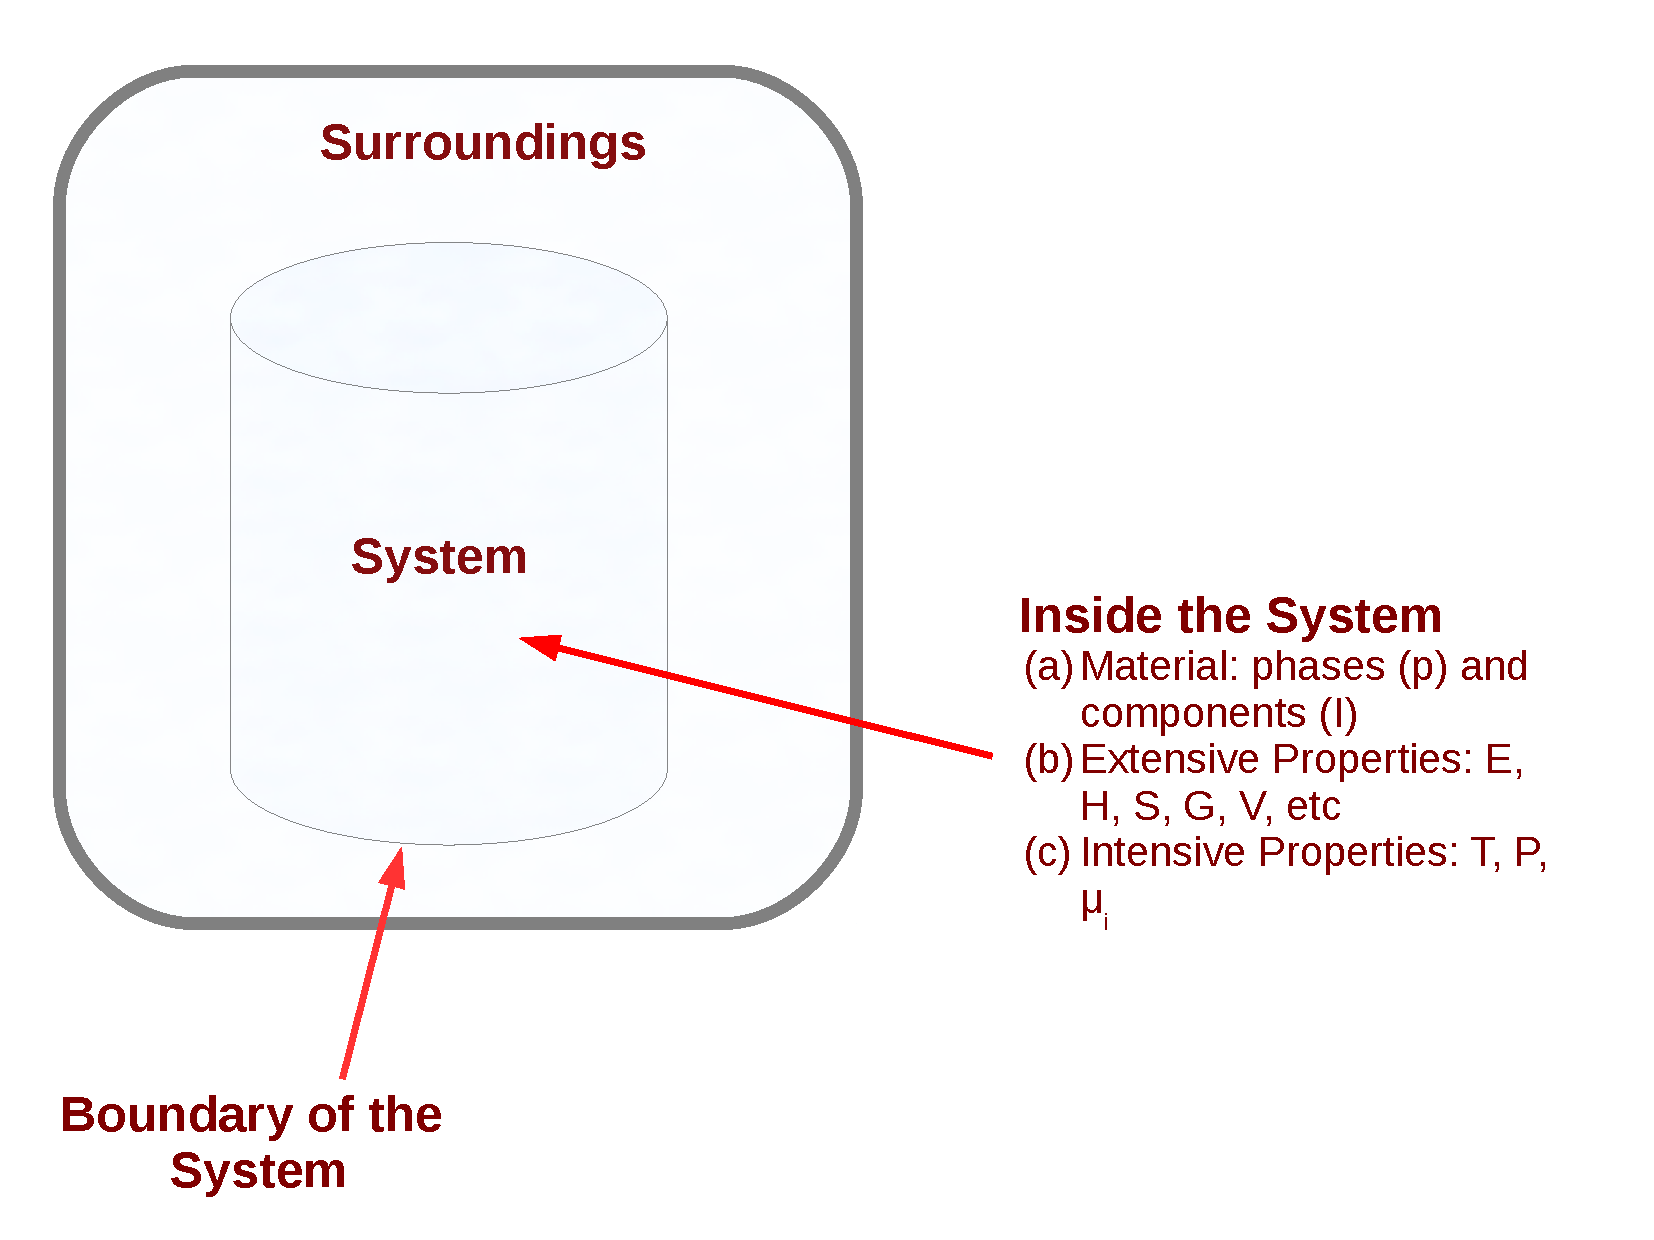
\includegraphics[width=8cm, height=8cm]{./Pics/Fig_SystemDefinition}
       \caption{Elements of a thermodynamic problem: system and surroundings separated by well-defined borders.}\label{Chapter:Introduction:Fig:Domain}
     \end{center}
   \end{figure}
   
   
%%% Subsection
   \subsection{System, Surroundings and Boundaries}\label{Chapter:Introduction:Section:Introduction:SystemSurroundingsBoundaries}\index{System}\index{System!Boundaries}\index{System!Surroundings}
   In practice, any thermodynamic analysis starts by defining the domain of interest, which can be a volume in space or quantity of matter (Fig.~\ref{Chapter:Introduction:Fig:Domain}). This domain is called {\it system}, \ie any 3-D region of physical space with prescribed mass; the remaining of the domain is called {\it surroundings} (or {\it neighbourhood}) which is limited by {\it boundaries}. The {\it boundary} is a surface that encloses the {\it system} and separates it from the {\it surroundings}. For example, in Fig.~\ref{Chapter:Introduction:Fig:Domain2}, liquid nitrogen is contained in a cylinder with prescribed wall thickness. In this case, the interior of the vessel with N$_{2}$ is the {\it system}, whereas the cylinder wall is the border of the system. 
% Figure
   \begin{wrapfigure}{I}{0.5\columnwidth}
        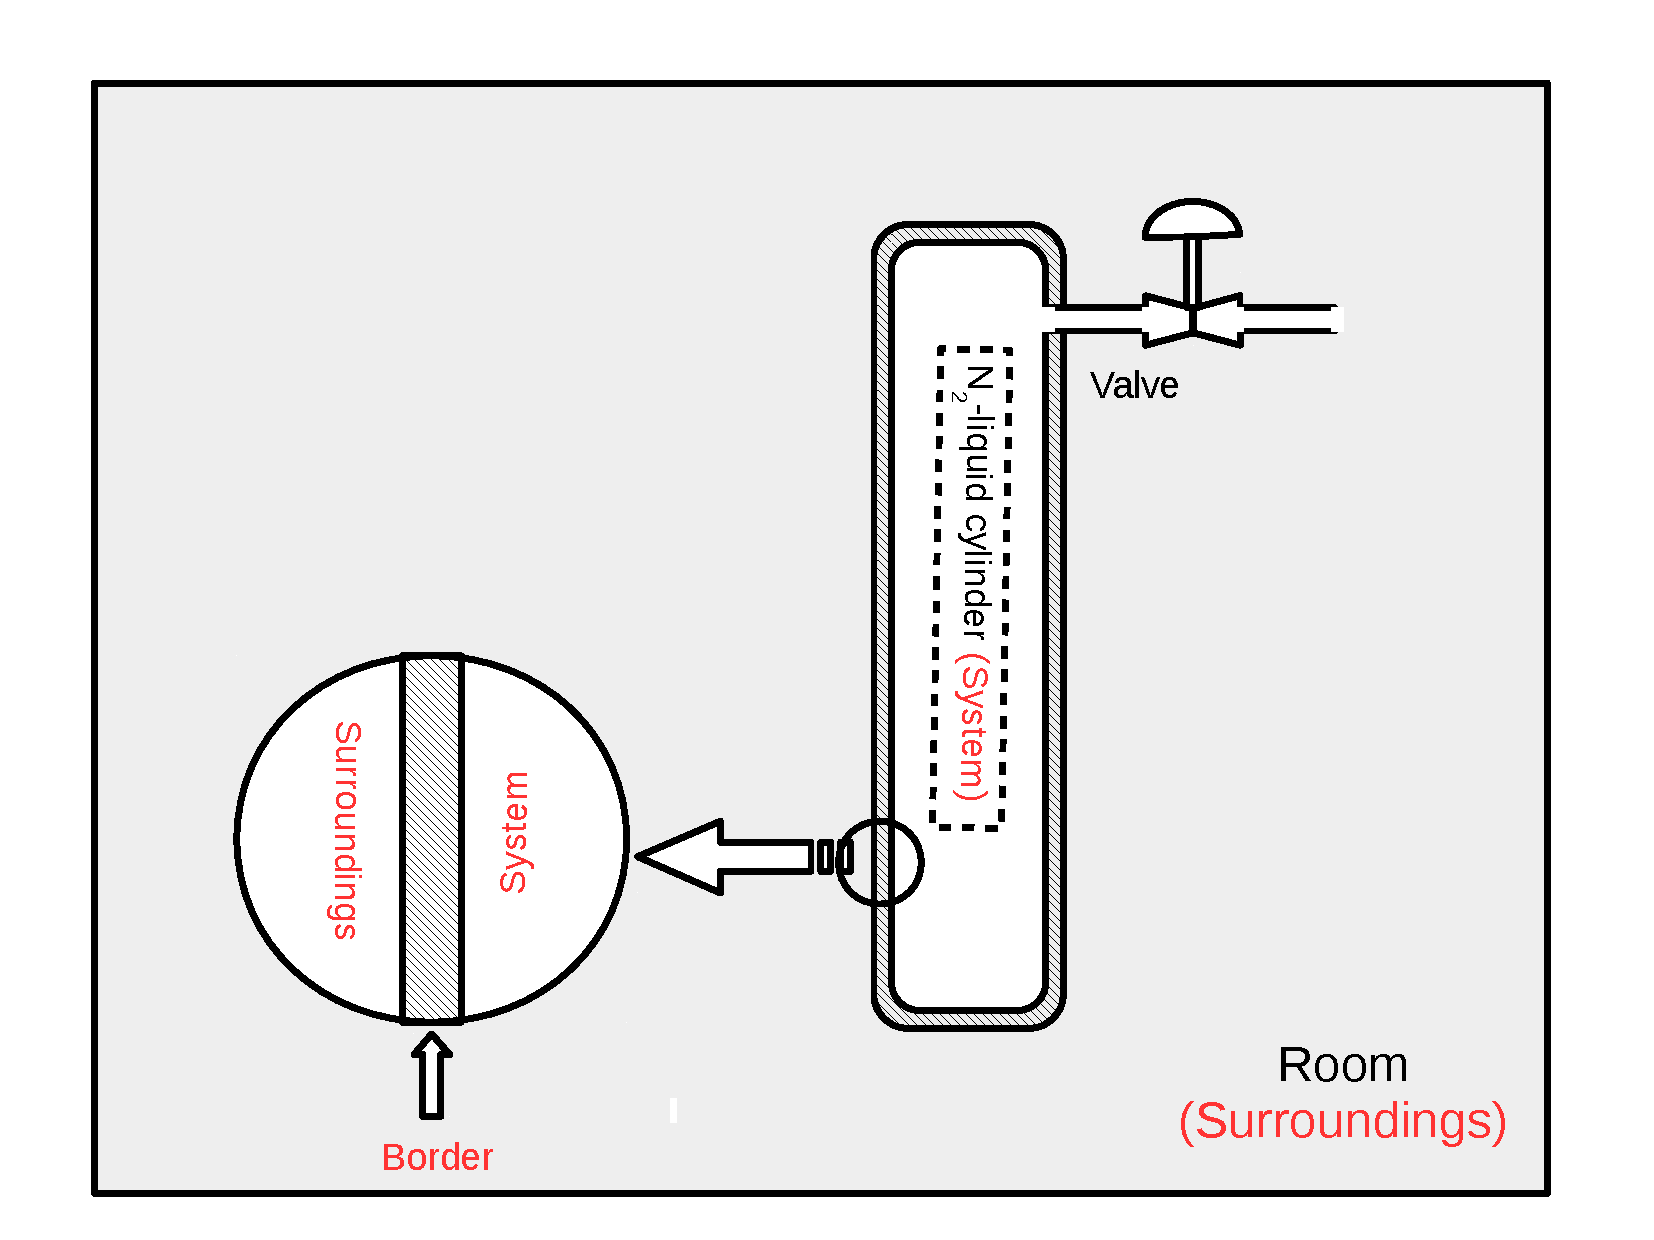
\includegraphics[width=0.4\columnwidth,clip]{./Pics/Fig_SystemDefinition2}
        \caption{Example of a well-defined thermodynamic problem: cylinder stored in a room. Pressurised liquid N$_{2}$ contained in a cylinder is the system, whereas the remaining of the room are the surroundings. Cylinder's wall is the border of the system.}\label{Chapter:Introduction:Fig:Domain2}
   \end{wrapfigure}

   For convenience, sometimes we may want to divide the {\it system} into multiple {\it sub-systems} and analyse them individually, or to combine several small {\it systems} into larger {\it super-systems}. The choice depends on the conditions of the domain of interest and how mass and energy flow across the {\it sub-systems}. For example, in Fig.~\ref{Chapter:Introduction:Fig:Domain2}, if the valve is opened to the room (at atmospheric pressure) $N_{2}$ would be vaporised ({\it phase change}) and occupy the whole room. In such scenario, the room and the cylinder become the {\it system} bounded by the room's walls; the area outside the room is now the surroundings. Multiple different configurations can be drawn from this rather simple cylinder-room set.

%%% Table
   \begin{table}[h]
     \begin{center}
      \begin{tabular}{|c|c|c|}
         \hline
                      & {\bf Mass} & {\bf Energy} \\
                      & {\bf Exchange} & {\bf Exchange} \\
         \hline
         {\bf Open}   & {\it yes}  & {\it yes}    \\
         {\bf Closed} & {\it no}   & {\it yes}    \\
         {\bf Isolated}&{\it no}   & {\it no}     \\
         \hline 
      \end{tabular}  
        \caption{System and control volumes: energy and mass transfer.}\label{Chapter:Introduction:Table:System}
     \end{center}
   \end{table}
   
   If mass and energy are allowed to flow across the {\it boundaries}, we say that the {\it system} is {\bf open}, otherwise if only the energy is allowed to flow (\ie be transferred) across the {\it boundaries}, the {\it system} is assumed to be {\bf closed}. If both energy and mass can not be transferred across the {\it boundaries} the system is assumed {\bf isolated}, in such case, where there is no energy flow, the boundary is called {\bf adiabatic} (Table~\ref{Chapter:Introduction:Table:System}).\index{System!Open}\index{System!Closed}\index{System!Isolated}\index{System!Adiabatic}\index{Adiabatic}

% Figure
   \begin{figure}[h]
     \begin{center}
        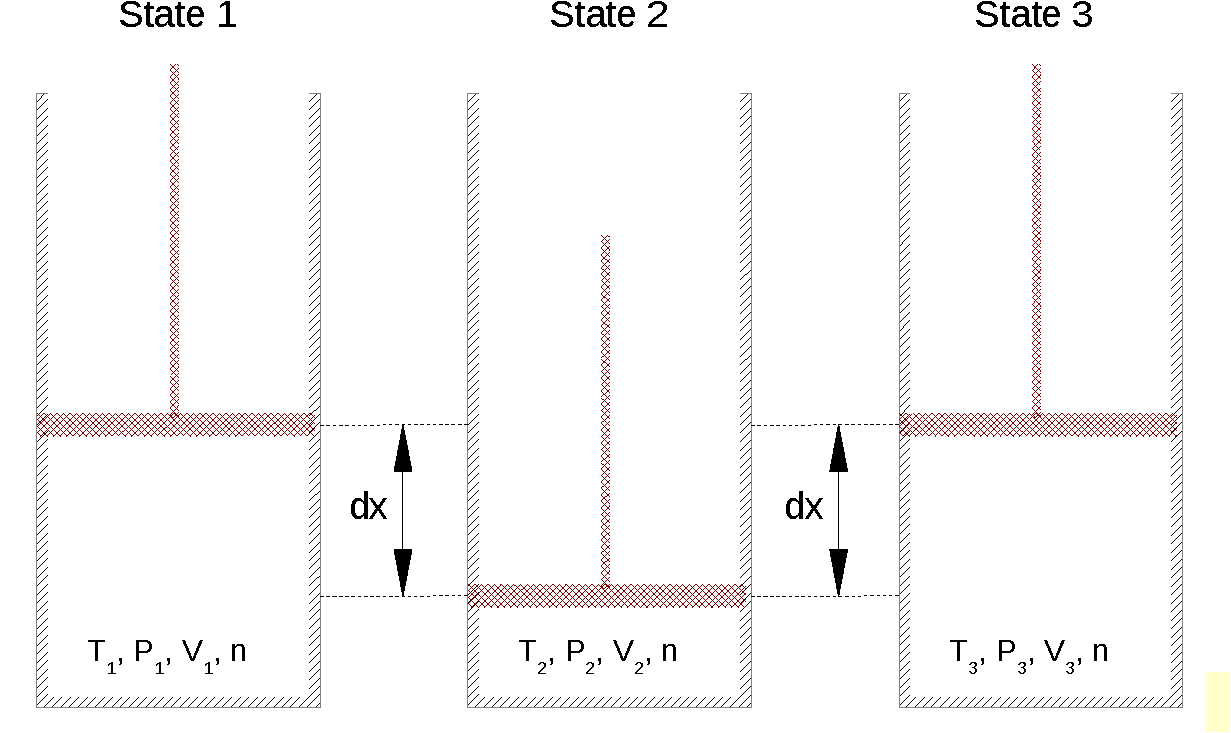
\includegraphics[width=0.7\columnwidth,clip]{./Pics/Fig_SystemDefinition3}
        \caption{Cylinder-piston system with extensive/intensive properties.}\label{Chapter:Introduction:Fig:Domain3}
     \end{center}
   \end{figure}

   In the example depicted in Fig.~\ref{Chapter:Introduction:Fig:Domain2}, assuming an ordinary industrial liquid N$_{2}$ (at subzero temperature) cylinder, if the valve is closed, then there is no fluid flow from the cylinder to the room, but heat is flowing from the environment to the cylinder cavity. Such system is said to be {\bf closed}.
   
\medskip
% Example
\begin{MyExample}{\begin{center}{\bf Example}\end{center}}
\begin{example}\label{Chapter:Introduction:Example1}
  \citep{Reisel_Book} For the following systems, determine whether the system described is best modelled as an isolated, closed or open system:
  \begin{enumerate}[a)]
     \item steam flowing through a turbine\;\;$\rightarrow$\;\; {\it Open.}
     \item an incandescent light bulb\;\;$\rightarrow$\;\; {\it Closed.}
     \item an inflated tire\;\;$\rightarrow$\;\; {\it Isolated if the tire is at rest, but closed if it is in movement.}
     \item a rock formation 200 m below the surface of the earth\;\;$\rightarrow$\;\; {\it Open.}
     \item a tea kettle containing boiling water\;\;$\rightarrow$\;\; {\it Open as water steam can still leave the system.}
     \item a human body\;\;$\rightarrow$\;\;{\it Depending on the circumstances, a human body can be either open (\eg during meals, physical exercises etc) or closed.}
     \item an engine's radiator\;\;$\rightarrow$\;\; {\it Closed}.
  \end{enumerate}
\end{example}
\end{MyExample}

%%% Subsection
   \subsection{Properties and State of Substances}\label{Chapter:Introduction:Section:Introduction:ExtensiveIntensiveProperties}\index{Extensive Properties}\index{Intensive Properties}\index{System!Extensive Properties}\index{System!Intensive Properties}
   The {\it material} in a system is composed of phases (e.g., solid, liquid, gas) with distinct physical and chemical properties, thus with explicit {\it boundaries} (\ie interfaces) between phases. {\it State} is the condition of the system at an instant of time and described by its properties.  From this definition of state, any property has a single value at each state. A quantitative property of a system (\eg temperature and pressure) describes macroscopic characteristics, which may vary with time (\ie time-dependent property). Two states of the matter are equivalent if they have the same properties, \eg in a cylinder-piston system (Fig.~\ref{Chapter:Introduction:Fig:Domain3}) containing {\it n} moles of pure gas, if {\it state 1} is defined by temperature $T_{1}$, pressure $P_{1}$ and volume $V_{1}$, and {\it state 3} is defined by temperature $T_{3}$, pressure $P_{3}$ and volume $V_{3}$, state 1 is {\it equivalent} to state 3 {\it if and only if} $T_{1} = T_{3}$ and $P_{1} = P_{2}$. 
\medskip

   Thermodynamic properties may be classified as either {\bf extensive} or {\bf intensive}. An extensive property is a property that depends on the mass (or extent) of the substance (\ie size) in the system. Examples of extensive properties are total mass, total volume, total internal energy etc. An intensive property is a property that is independent of the mass of the substance, examples are temperature and pressure.
% Figure
   \begin{wrapfigure}{R}{0.5\columnwidth}
        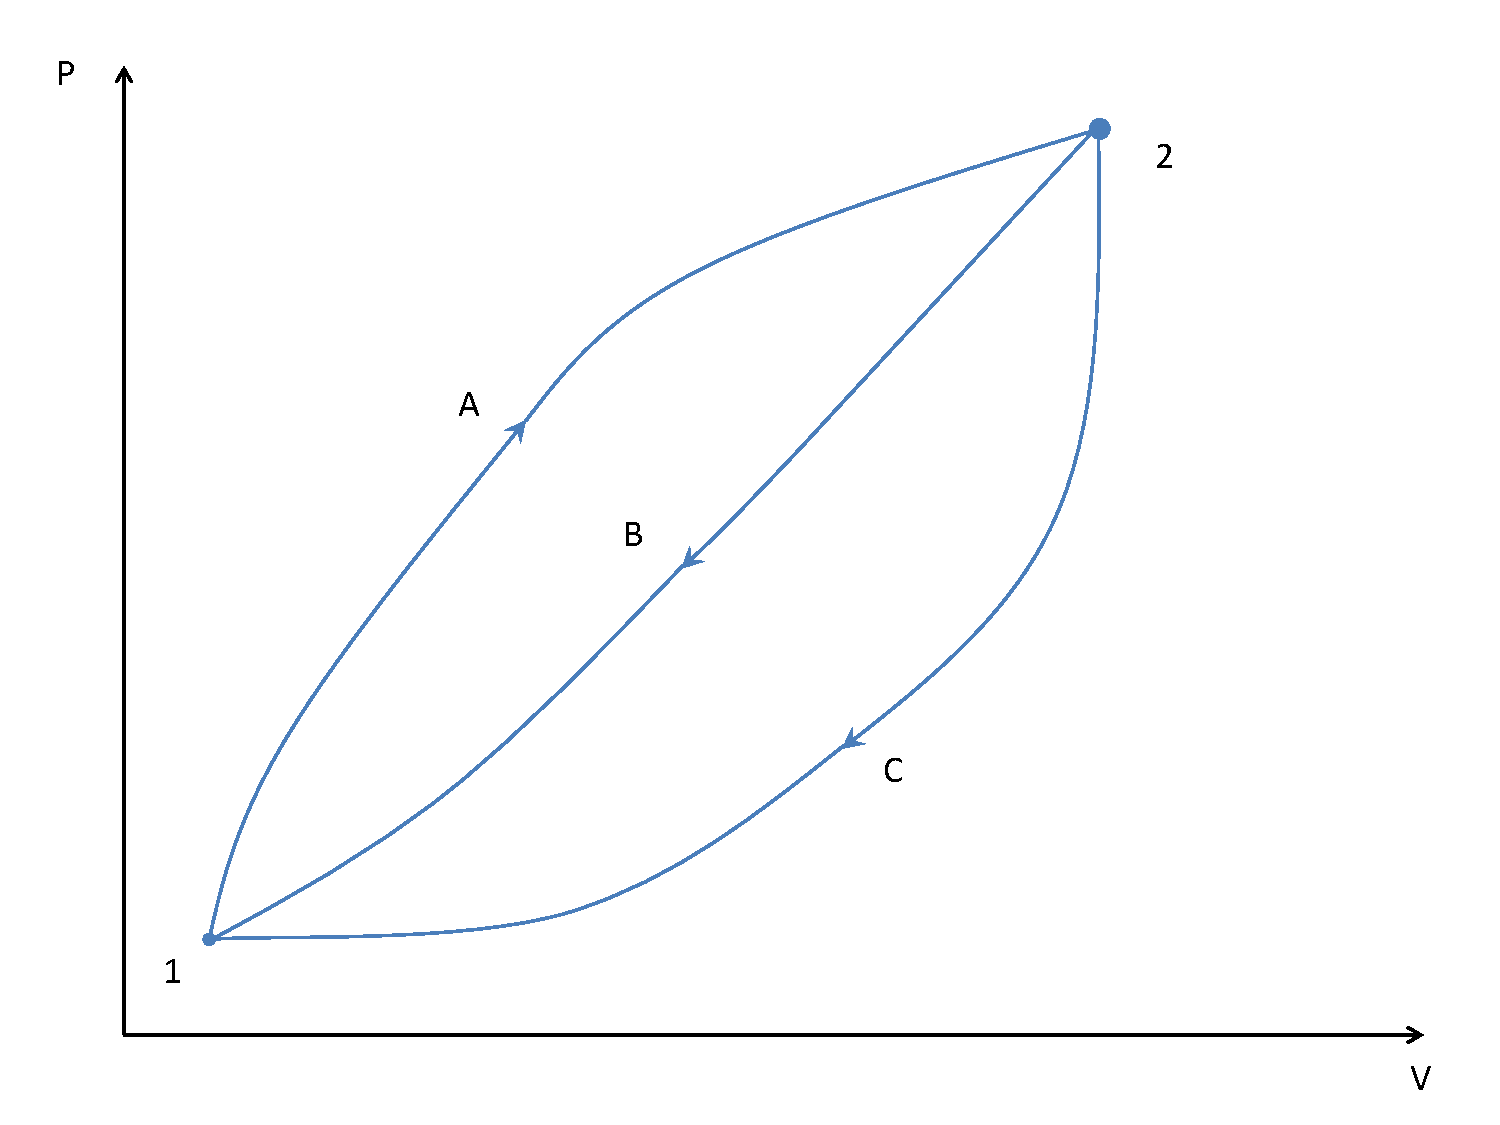
\includegraphics[width=0.4\columnwidth,clip]{./Pics/first_law_process}
        \caption{Schematic representation of cycles.}\label{Chapter:Introduction:Fig:CyclesSchematic}
   \end{wrapfigure}

   Thus, for example, if a system is cut in half, its intensive properties remain unchanged, while extensive properties are cut in half. The ratio of an extensive property to the mass (\ie property per unit mass) is called {\bf specific property}, and this is an {\bf intensive} property.. The ratio of an extensive property to the number of moles of the substance in the system (\ie property per mole) is referred as {\bf molar property}, this is also an {\bf intensive} property.

%%% Subsection
   \subsection{Processes and Cycles}\label{Chapter:Introduction:Section:Introduction:ProcessesCyclesDefinition}\index{Process}\index{Cycle}
   A process occurs when the system undergoes a change in a state or a transfer of energy at a steady-state. For example, let's consider the cylinder-piston system (Fig.~\ref{Chapter:Introduction:Fig:Domain3}) at state 1. As mechanical energy is transferred from the surroundings through a force (represented by an external pressure) exerted on the piston, the state of the system changes from {\it 1} to {\it 2}. A {\it quasi-static process}\index{Process!Quasi-Static} (also called reversible process) is a succession of equilibrium states at infinite slowness $\left(\Delta\text{t}\rightarrow\text{0}\right)$.
   
   {\it Cycles} are defined as any process (or a set of processes) in which the end states are identical. For example, in the processes (closed system) depicted in Fig.~\ref{Chapter:Introduction:Fig:CyclesSchematic}, the system is initially at state 1 $\left(\text{with coordinates } P_{1}\text{ and }V_{1}\right)$ and driven (by simultaneous changes in pressure, volume and temperature) to the state 2 through pathway $A$. After a while, the system is restored to the original state $1$ through pathway $B$. These two processes, $A$ and $B$, constitute a cycle as the final state is the same as the initial state.   
   
%%%
%%% SECTION
%%%
   \section{Thermodynamic Work and Heat}\label{Chapter:Introduction:Section:ThermodynamicWorkHeat}\index{Work}\index{Heat}\index{Energy}
   \begin{subequations}
     Work can be defined as a form of energy transfer due to changes in external macroscopic physical properties of a thermodynamic system. It can be expressed in several forms: magnetic, mechanical, electrical etc. For example, in a piston-cylinder system (Fig.~\ref{Chapter:Introduction:Fig:Domain3}) work is produced by the system when the gas volume expands against an external force (states 2-3). Similarly, an external force is responsible for the compression of the gas, \ie work is given to the system (states 1-2). In these cases (expansion and compression of a gas), the transfer of work (to or from the system) is due to the application of a finite force on the system boundary (piston).

     It is clear that the boundary (\ie volume limited by the cylinder wall and the piston-head) either contracts or expands due to external and internal forces acting on it. In other words, applied forces acting over a distance (piston length) result in mechanical energy transfer (\ie work). For an infinitesimal displacement of the piston within a cylinder, {\it dx}, the work ($W$) can be defined by
     \begin{equation}
        dW = F dx,\label{Chpt01_Work1}
     \end{equation}
     where $F$ is the force acting vertically upon the piston. If the movement occurs over a finite distance, the resulting work can be obtained by integrating Eqn.~\ref{Chpt01_Work1}. By convention, {\bf work} is assumed {\bf positive} if the displacement is in the same direction as the force applied, and {\bf negative} when the force and the displacement are in opposite directions. Thus, from stages 2 to 3 (Fig.~\ref{Chapter:Introduction:Fig:Domain3}), the force is acting upon the piston with contraction of the volume of the gas $\left(V^{t}\right)$,
     \begin{displaymath}
       dW = -PAd\left(\frc{V^{t}}{A}\right),
     \end{displaymath}
     where $A$ is the area of the piston (constant) and $P=F/A$ is the pressure exerted on the piston, then
     \begin{shaded}
        \begin{equation}
           dW = -PdV^{t}.\label{Chpt01_Work2}
        \end{equation}
     \end{shaded}
     Equation~\ref{Chpt01_Work2} describes the work undertaken by any process when the volume changes due to transfer of energy from or to the system. If the fluid undertakes a compression (thus reduction of volume) due to pressure over the system, the work is positive, otherwise when the system produces work (\ie transfer energy to the surroundings through expansion of the boundaries), the work is considered as negative. The concept of work leads to the definition of {\bf energy} as the capacity of the system to produce work.

     \citet{Devoe_Book} defined {\bf heat} as `the transfer of energy across the boundary caused by a temperature gradient at the boundary'. This concept will naturally lead to the {\it First Law of Thermodynamics} (Chapter~\ref{Chapter:FirstLaw}).     

   \end{subequations}
   
%%%
%%% SECTION
%%%
   \section{Thermodynamic Equilibrium and the Zeroth Law}\label{Chapter:Introduction:Section:Equilibrium_ZerothLaw}\index{Equilibrium!Mechanical}\index{Equilibrium!Chemical}\index{Equilibrium!Thermal }\index{Laws of Thermodynamics!Zeroth law}
   During thermodynamic processes, the state of the system may change due to gradients of different variables within or across boundaries, \ie
   \begin{enumerate}[a)]
        \item pressure gradients result in momentum transfer and/or convective mass transport;
        \item temperature gradients produce heat exchange, and;
        \item concentration gradients yields to diffusive mass transfer.
   \end{enumerate}
   Changes in the state of the system will continue until all internal or cross-boundary gradients vanish. When all gradients are non-existent the system exhibits no further changes and at such conditions, the system is said to be in {\bf thermodynamic equilibrium}.\index{Equilibrium!Thermodynamic}
      A system is in {\bf thermodynamic equilibrium} if it satisfies the criteria for mechanical, thermal and chemical equilibrium.  
% Figure
   \begin{wrapfigure}{I}{0.5\columnwidth}
        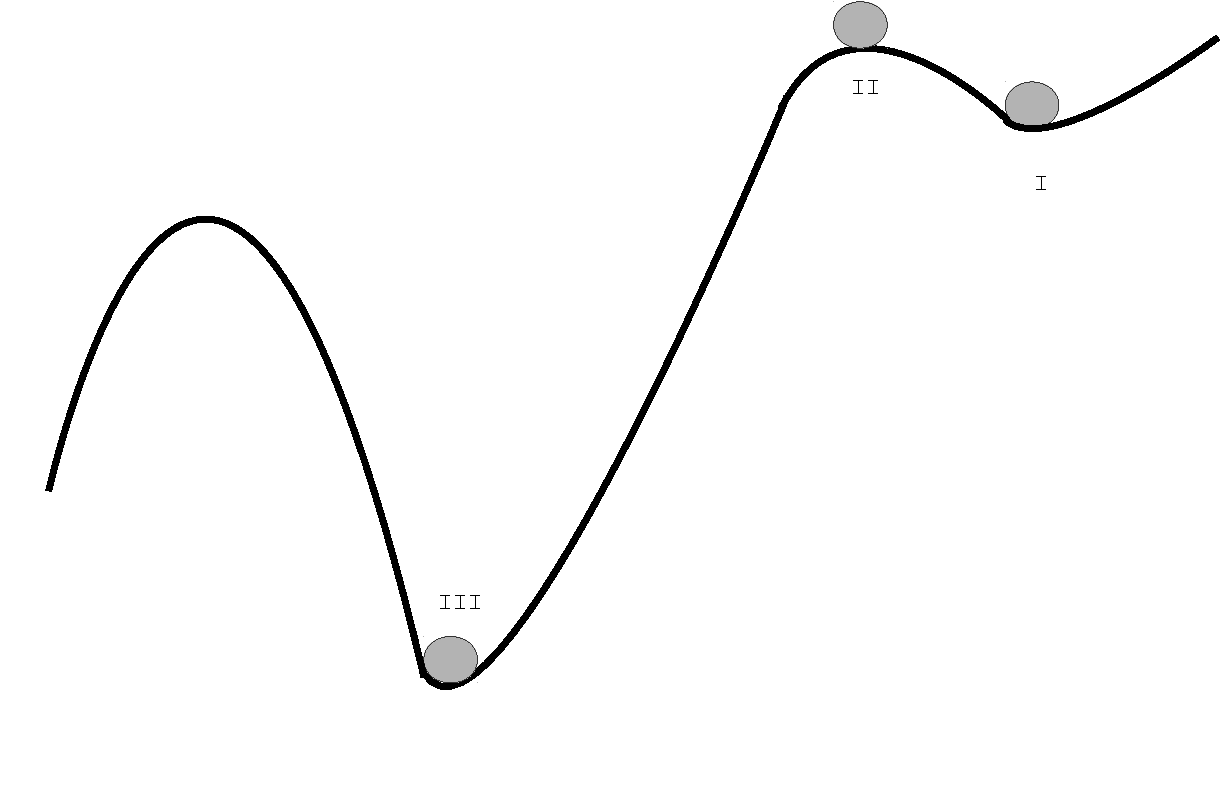
\includegraphics[width=0.4\columnwidth,clip]{./Pics/Fig_SystemDefinition4}
        \caption{Potential energy variation in a particle motion.}\label{Chapter:Introduction:Fig:Domain4}
   \end{wrapfigure}

   Let's consider a particle initially at rest (state I in Fig.~\ref{Chapter:Introduction:Fig:Domain4}). The total energy associated with this particle is the sum of potential and kinetic energies (assuming that the particle is chemically inert and is kept at a constant temperature). If the particle is perturbed by a mechanical force of very small magnitude, it will eventually return to its initial state (\ie at a finite time), however if the perturbation is sufficiently large the particle is unlikely to return to the original state. In this scenario, the particle is said to be in a {\it unstable equilibrium}\index{Equilibrium!Mechanical!Unstable}. Now, let's assume that the particle is at state II, where any perturbation can move it to either state I or III. In such conditions, the particle is said to be in a {\it meta-stable equilibrium}\index{Equilibrium!Mechanical!Meta-stable}. Finally, if the particle is at state III, it will remain at this condition even under the influence of large perturbation. At such conditions, the particle is said to be in a {\it stable equilibrium}\index{Equilibrium!Mechanical!Stable}. If $E_{p}$ is the potential energy of the particle and $x$ is the displacement in the vertical direction, the equilibrium states can be described as
   \begin{equation}
      \begin{cases}
         \text{Stable equilibrium (III):}  & \frc{\partial E_{p}}{\partial x} = 0 \text{ and } \frc{\partial^{2} E_{p}}{\partial x^{2}} > 0; \\
          \\
         \text{Unstable equilibrium (II):}  & \frc{\partial E_{p}}{\partial x} = 0 \text{ and } \frc{\partial^{2} E_{p}}{\partial x^{2}} < 0; \\
          \\
         \text{Meta-stable equilibrium (I):}  & \frc{\partial E_{p}}{\partial x} = 0 \text{ and } \frc{\partial^{2} E_{p}}{\partial x^{2}} = 0; \\
      \end{cases}
   \end{equation}
   These mechanical equilibrium states can be extended to thermodynamic systems during phase changes, where the potential energy and the spatial coordinate are replaced by the {\it Gibbs free energy} and intensive/extensive properties, respectively.

   \bigskip

   The concept of thermal equilibrium is intuitively simple: if two or more bodies at distinct temperatures are in physical contact, the bodies will tend to a single temperature at a finite time. This principle is called the {\bf Zeroth Law} of thermodynamics and was first stated by J. C. Maxwell in 1872:
   \begin{MyBlock}{{\bf Zeroth Law of Thermodynamics (Maxwell, 1872) } }
     ``Bodies whose temperatures are equal to that of the same body have themselves equal temperatures.”
   \end{MyBlock}
   This definition enables the use of thermometers as devices to measure the temperature of bodies. Traditional thermometers have two components, a bulb containing mercury and a linear temperature scale. The mercury bulb is maintained at a relatively low temperature $\left(\text{\ie } T_{\text{th}}\le 35^{\circ}\text{C}\right)$, whereas a body is at temperature $T>T_{\text{th}}$. When the thermometer and the body are in contact, from the {\it zeroth law}, both will reach the same temperature $T$ at a finite time. The temperature difference triggers a volumetric expansion of the mercury that can be readily observed in the scaled glass column.

\clearpage   
\begin{FinalSummaryBlock}{Summary}
    In this chapter, some fundamental concepts of thermodynamic properties were revised and the their relationships with energy were introduced, also:
    \begin{itemize}
       \item Thermodynamics is the study of the transformations of energy;
       \item Energy can be defined as the capacity to produce work;
       \item Work is the transfer of energy by motion against an opposing force (Eqns.~\ref{Chpt01_Work1}-\ref{Chpt01_Work2};
       \item Heat is the transfer of energy  as a result of a temperature difference between the system and the surroundings;
       \item Definitions of system, surroundings and boundaries were stated in Section~\ref{Chapter:Introduction:Section:Introduction:SystemSurroundingsBoundaries};
       \item In open systems, mass and energy are allowed to freely flow across the boundaries of the system, whereas in closed system only energy is able to cross the borders at constant mass. In isolated (or adiabatic) system, neither energy nor mass can be trabsported across the borders;
       \item A state function is a property that depends only on the current state of the system and is independent of the origin of the state; 
       \item Thermal equilibrium is a condition in which no change of state occurs when two (or more) bodies are in contact with each other;
       \item Mechanical equilibrium is the condition of equality of pressure across the boundary of the system;
       \item The Zeroth Law of thermodynamics states that if a body {\it A} is in thermal equilibrium with a body {\it B}, and {\it B} is in thermal equilibrium with {\it C}, then {\it C} and {\it A} are also in thermal equilibrium;
    \end{itemize} 
   
     Most of these fundamentals concepts are familiar to you through other engineering courses. However, the remaining of this document strongly relies on this concepts and ideas, and you should understand all these concepts before moving forward.
\end{FinalSummaryBlock}

%\begin{MyTutorial}{\begin{center}{\bf Tutorial}\end{center}}
%  \begin{problem}
%  \end{problem}
%\end{MyTutorial}
 % Introduction and Review of Basic Concepts of Thermodynamics
     \setcounter{examplecounter}{0}

  
%%%
%%% CHAPTER
%%%
\chapter{Introduction to Properties of Gases}\label{Chapter:Intro_Property_of_Gases}

   \begin{LearningObjectivesBlock}{Learning Objectives}
      Upon completion of this chapter, you will be able to
        \begin{enumerate}
           \item define ideal gas and identify the main assumptions;
           \item differentiate an ideal from a real gas through state conditions;
           \item explain Boyle's, Gay-Lussac's and Charles' laws for ideal gases;
           \item define and explain the equation of state for ideal gases;
           \item state the Dalton's law for gaseous mixtures.
        \end{enumerate}
\medskip
     Recommended reading: Chapter 1 of \citet{Atkins_Book,Adamson_BookChapter}.
   \end{LearningObjectivesBlock}


%%%% ETOC
\localtableofcontents
   
%%%
%%% SECTION
%%%
     \section{Introduction}\label{Chapter:Intro_Property_of_Gases:Section:Intro}

   The physical condition (\ie state) of a substance is defined by its physical properties. For example, the state of a pure fluid is specified by volume ($V$), mass (through the number of moles, $n$), pressure ($P$) and temperature ($T$). Laboratory experiments with fluids revealed that if three of these properties (\eg $V, n, T$) are specified, the state of the fluid is naturally defined, and the forth property (\ie $P$) is fixed. Mathematically, this can be represented by a functional often referred as {\bf equation of state}\index{Equation of State} (EOS)\index{EOS|see {Equation of State}},
     \begin{displaymath}
       P = f(T,V,n),
     \end{displaymath}
     which states that if $T$, $n$ and $V$ are known for a particular fluid, then the pressure of the system for the fluid at this state can be readily determined. The state and properties of any chemical species can be described by an specific equation of state\footnote{Equations of state are the main focus of Chapter~\ref{Chapter:VolumetricPropertiesPureSubstances}.}.
   
%%%
%%% SECTION
%%%
     \section{Ideal Gases}\label{Chapter:Intro_Property_of_Gases:Section:IdealGases}\index{Gases!Ideal gas}
     \begin{subequations}

     \noindent A fluid is assumed to behave as an {\it ideal gas} if the following two assumptions are true:
     \begin{enumerate}[i)]
       \item molecules of gases are considered as {\bf massless} particles;
       \item there are {\bf no} interaction between the gas particles due to,
         \begin{enumerate}[a)]
           \item volume of the molecules is negligibly small compared with the volume occupied by the gas, and/or;
           \item the distance between gaseous molecules are infinitely large $\left(d\rightarrow \infty\right)$, except during elastic collisions over negligible duration.
         \end{enumerate}
     \end{enumerate}
     \noindent These lead to an obvious conclusion that for a gas to behave as an ideal gas the pressure should be infinitely small, \ie $P\rightarrow 0$. In practical engineering calculations, we assume that a fluid behaves as an ideal gas at low to moderate pressures. The $PVT$ behaviour of fluids was initially investigated through experimental observations of gases at low pressures that led to three intuitive relationships:
     \begin{itemize}
       \item For isothermal processes in closed systems (\ie $T$ and $n$ are constant), $P$ and $V$ are inversely proportional to each other, \ie an increase in pressure leads to a decrease in volume,
          \begin{displaymath}
             P \propto \frc{1}{V},
          \end{displaymath}          
%          
       \item For isochoric processes in closed systems (\ie $V$ and $n$ are constant), $T$ and $P$ are directly proportional to each other, \ie an increase in temperature leads to an increase in pressure,
          \begin{displaymath}
            T \propto P,
          \end{displaymath}         
%
       \item For isobaric processes in closed systems (\ie $P$ and $n$ are constant), $T$ and $V$ are directly proportional to each other, \ie an increase in temperature leads to an increase in volume.
          \begin{displaymath}
            T\propto V.
          \end{displaymath}          
     \end{itemize}
     \begin{shaded}
        These proportionality relations can be merged into a single expression,\index{Gases!Boyle's law}\index{Gases!Gay-Lussac's law}\index{Gases!Charles' law}\index{Gay-Lussac's law|see {Gases}}\index{Charles' law|see {Gases}}\index{Boyle's law|see {Gases}}
          \begin{equation}
            \frc{P V}{n T} = R \;\;\Longleftrightarrow \;\;
              \begin{cases}
                P_{1}V_{1} = P_{2}V_{2}, & \text{if } T \text{ and } n \text{ are constant (Boyle's law)},  \\
         \\
                P_{1}T_{1}^{-1} = P_{2}T_{2}^{-1}, & \text{if } V \text{ and } n \text{ are constant (Gay-Lussac's law)}, \\
         \\
                V_{1}T_{1}^{-1} = V_{2}T_{2}^{-1}, & \text{if } P \text{ and } n \text{ are constant (Charles' law)}.
             \end{cases}\label{Chapter:Intro_Property_of_Gases:Eqn:IdealEOS}\index{Equation of State!Ideal gas}
          \end{equation}
        The constant of proportionality, $R$, which is found experimentally to be the same for all gases, is called {\bf universal gas constant} (Table~\ref{Chapter:Intro_Property_of_Gases:Table:RConst}). This expression, 
          \begin{equation}
             P=\frc{n R T}{V},\label{Chapter:Intro_Property_of_Gases:Eqn:IdealEOS}\index{Equation of State!Ideal gas}
          \end{equation}\index{Equation of State!Ideal gas}
        is called {\bf ideal gas equation of state} and becomes increasingly accurate for any gas as pressure tends to zero $\left(P\rightarrow 0\right)$.
     \end{shaded}
     \end{subequations}
     
   \begin{table}[h]
     \begin{center}
     \begin{tabular}{||c c||}
       \hline\hline
           $\mathbf{R}$   & {\bf Units} $\mathbf{\left(\text{V.P.T}^{-1}\text{n}^{-1}\right)}$ \\
           \hline\hline
           8.3145    &  J.K$^{-1}$.mol$^{-1}$  \\
           8.3145    &  kJ.K$^{-1}$.kmol$^{-1}$  \\
           8.3145    &  l.kPa.K$^{-1}$.mol$^{-1}$  \\
           8.3145$\times$10$^{-3}$    & cm$^{3}$.kPa.K$^{-1}$.mol$^{-1}$  \\
           8.3145    &  m$^{3}$.Pa.K$^{-1}$.mol$^{-1}$  \\
           8.3145$\times$10$^{-5}$    &  m$^{3}$.bar.K$^{-1}$.mol$^{-1}$  \\
           8.2057$\times$10$^{-2}$ &  l.atm.K$^{-1}$.mol$^{-1}$  \\
           \hline\hline           
     \end{tabular}
     \caption{Gas constant, $R$.}\label{Chapter:Intro_Property_of_Gases:Table:RConst}\index{Universal gas constant}\index{R|see {Universal gas constant}}\index{Gas constant|see {Universal gas constant}}
     \end{center}
   \end{table}
   
   % Example
   \begin{MyExample}{\begin{center}{\bf Example}\end{center}}
     \begin{example}\label{Chapter:Intro_Property_of_Gases:Example1}
       In an industrial process, nitrogen is heated to 650.15 K in a vessel of constant volume. If it enters the vessel at 43 atm and 298.15 K, what pressure would it exert at the working temperature if it behaved as an ideal gas?

       {\it This problem deals with a gas that undertakes an isochoric (\ie constant volume) process. Nitrogen gas at $P_{1} = 43$ atm and $T_{1} = 298.15$ K is compressed to pressure $P_{2}$ 'till temperature reaches $T_{2} = 650.15$ K.

         Using the ideal gas equation for states 1 and 2,}
       \begin{eqnarray}
         && \left(\frc{PV}{nT}\right)_{1} = R = \left(\frc{PV}{nT}\right)_{2},\;\;\;\text{ with } V_{1}=V_{2} \text{ and }\;\; n_{1}=n_{2}\nonumber \\
         && \frc{P_{1}}{T_{1}} = \frc{P_{2}}{T_{2}} \;\;\Rightarrow \;\; P_{2}= 93.7664 \text{ atm } \nonumber
         \end{eqnarray}
     \end{example}
   \end{MyExample}

\medskip
   % Example
   \begin{MyExample}{\begin{center}{\bf Example}\end{center}}
     \begin{example}\label{Chapter:Intro_Property_of_Gases:Example2}
       500 kg of helium gas is stored in a tank at 50$^{\circ}$C and 2.5 bar. The fluid is then transferred to a pressure vessel where it is isothermically compressed to 73 bar.  What is the volume occupied by {\it He} in such conditions? Assume ideal gas behaviour. Molar mass ({\it MW}) of helium is 4.0026 g.mol$^{-1}$.

       {\it In this problem, we need to calculate the volume of helium at the pressure vessel after isothermal compression. However, not all necessary conditions are known, \ie}
       \begin{displaymath}
         \frc{P_{1}V_{1}}{n_{1} R T_{1}} = \frc{P_{2}V_{2}}{n_{2} R T_{2}} \Longrightarrow P_{1}V_{1} = P_{2}V_{2},\;\;\;\;\text{where }R\text{ and } n_{i}\text{ are constants},
       \end{displaymath}
           {\it thus there is 1 equation and 2 unknowns, $V_{1}$ and $V_{2}$. In order to solve this problem, we need to first compute $n_{1}$ and $V_{1}$ via, }
           \begin{displaymath}
              V_{1} = \frc{n_{1}R T_{1}}{P_{1}} = 1342.5427\;\text{m}^{3},\;\;\;\text{ where } n_{1} = \frc{m_{1}}{MW_{1}} =  124918.8028\text{ moles}.
           \end{displaymath}
           {\it With $V_{1}$, we can now calculate the volume after compression, $V_{2}$}
           \begin{displaymath}
              P_{1}V_{1} = P_{2}V_{2} \;\;\; \Longrightarrow\;\;\; V_{2} = 45.9775 \text{m}^{3}
           \end{displaymath}
           
     \end{example}
   \end{MyExample}
   
   % Example
   \begin{MyExample}{\begin{center}{\bf Example}\end{center}}
     \begin{example}\label{Chapter:Intro_Property_of_Gases:Example3}
       \citep{Atkins_Book} 
       \begin{enumerate}[a)]
           \item Deduce a relation between pressure and mass density $\left(\rho\right)$ of an ideal gas of molar mass $MW$;
           \item After careful measurement of the density of dimethyl ether at relatively low pressure conditions, a chemical engineering student obtained the following experimental data at 25$^{\circ}$C,
               \begin{center}
                  \begin{tabular}{c c c c c c}
                     $\mathbf{P}$ [kPa]  & 12.223 & 25.20 & 36.97 & 85.23 & 101.3 \\
                     $\mathbf{\rho}\;\left[\text{kg.m}^{-3}\right]$ & 0.225  &  0.456  &  0.664 & 1.468 & 1.734  
                  \end{tabular}
               \end{center}
               Obtain the molar mass of dimethyl ether at each pressure coordinate and compare with the real value of 46.07 g.mol$^{-1}$. What conclusions could be drawn from this data?
       \end{enumerate}
\medskip

       \begin{enumerate}[a)]
           \item {\it The first part of the problem requires the development of a mathematical relation between $P$ and $\rho$. Defining} $\rho=\frc{m}{V}$ {\it which can be allocated in the ideal EOS} $\left(\text{ and }n=\frc{m}{MW}\right)$,
              \begin{eqnarray}
                 P &=& \frc{n R T }{V} = \frc{m}{MW}\frc{R T}{V} \nonumber\\ 
                   &=& \frc{\rho R T}{MW}\nonumber
              \end{eqnarray}
%
           \item {\it We can use the relation derived in part (a) to calculate the molar mass of dimethyl ether at each pressure coordinate, thus}
              \begin{displaymath}
                  \begin{cases}
                     MW_{1} = \frc{\rho_{1} R T}{P_{1}} = \frc{0.225\text{ kg.m}^{-3}\cdot 8.3145\text{ m}^{3}\text{.Pa.}\left(\text{K.mol}\right)^{-1}\cdot 298.15\text{ K}}{12.223\times 10^{3}\text{ Pa}} = 45.6326 \text{ g.mol}^{-1} \\
                     MW_{2} = \frc{\rho_{2} R T}{P_{2}} = \frc{0.456\text{ kg.m}^{-3}\cdot 8.3145\text{ m}^{3}\text{.Pa.}\left(\text{K.mol}\right)^{-1}\cdot 298.15\text{ K}}{25.20\times 10^{3}\text{ Pa}} = 44.8575 \text{ g.mol}^{-1} \\
                     MW_{3} = \frc{\rho_{3} R T}{P_{3}} = \frc{0.664\text{ kg.m}^{-3}\cdot 8.3145\text{ m}^{3}\text{.Pa.}\left(\text{K.mol}\right)^{-1}\cdot 298.15\text{ K}}{36.97\times 10^{3}\text{ Pa}} = 44.5235 \text{ g.mol}^{-1} \\
                     MW_{4} = \frc{\rho_{4} R T}{P_{4}} = \frc{1.468\text{ kg.m}^{-3}\cdot 8.3145\text{ m}^{3}\text{.Pa.}\left(\text{K.mol}\right)^{-1}\cdot 298.15\text{ K}}{85.23\times 10^{3}\text{ Pa}} = 42.6977 \text{ g.mol}^{-1} \\
                     MW_{5} = \frc{\rho_{5} R T}{P_{5}} = \frc{1.734\text{ kg.m}^{-3}\cdot 8.3145\text{ m}^{3}\text{.Pa.}\left(\text{K.mol}\right)^{-1}\cdot 298.15\text{ K}}{101.3\times 10^{3}\text{ Pa}} = 42.4337 \text{ g.mol}^{-1} \\
                  \end{cases} 
              \end{displaymath}
              {\it We can compare these values with the real molar mass through the relative error ($\%$),}
                 \begin{displaymath}
                      \epsilon = \frc{\left| MW_{i} - MW^{\text{exp}}\right|}{MW^{\text{exp}}}\times 100,
                 \end{displaymath}
                 {\it leading to}
               \begin{center}
                  \begin{tabular}{c |c c c c c}
                     $\mathbf{P}$ [kPa]                            & 12.223  & 25.20   & 36.97   & 85.23   & 101.3    \\
                     $\mathbf{\rho}\;\left[\text{kg.m}^{-3}\right]$ &  0.225  &  0.456  &  0.664  &  1.468  &   1.734  \\
                     $\mathbf{MW}\;\left[\text{g.mol}^{-1}\right]$  & 45.6326 & 44.8575 & 44.5235 & 42.6977 &  45.4337 \\
                     $\mathbf{\varepsilon}\;\left[\%\right]$       &  0.9494 &  2.6319 &  3.3568 &  7.3199 &   7.8930
                  \end{tabular}
               \end{center}
               {\it From this data, it is clear that as $P\rightarrow 0$ dimethyl ether behaves similar to an ideal gas. However, as pressure increases the ideal gas EOS becomes less accurate.} 

                
       \end{enumerate}

           
     \end{example}
   \end{MyExample}
   

%%%
%%% SECTION
%%%
   \section{Gas Mixtures}\label{Chapter:Intro_Property_of_Gases:Section:MixtureGases}\index{Gases!Mixture}\index{Gases!Dalton's law}\index{Dalton's law|see {Gases}}\index{Pressure!Partial}\index{Partial pressure|see {Pressure}}

   \begin{subequations}
     Let's consider a gaseous mixture containing $\mathcal{N}$ chemical species. In several applications it is necessary to determine the pressure that each gas exerts in the whole system, \ie the contribution of each gas in the total pressure of the mixture. This contribution is often referred as {\it partial pressure}, $P_{i}$, of the gas {\it i} in a gas mixture and is defined as
     \begin{equation}
        P_{i} \equiv y_{i}P,\label{Chapter:Intro_Property_of_Gases:Eqn:PartialPressure_1}
     \end{equation}
     where $P$ is the total pressure and $y_{i}$ is the {\it mole fraction} of component $i$,\index{Mole fraction|see {Molar fraction}}\index{Molar fraction}
     \begin{displaymath}
        y_{i} = \frc{n_{i}}{n},\;\;\;\text{ with }\;\;i=1,\cdots,\mathcal{N}.
     \end{displaymath}
     The mole fraction is a normalised quantity and as such it must sum to unity, 
     \begin{displaymath}
        \summation[y_{i}]{i=1}{\mathcal{N}} = 1
     \end{displaymath}
     If we sum up the partial pressures of all components in the gaseous mixture, the total pressure of the system is recovered, \ie
     \begin{equation}
       \summation[P_{i}]{i=1}{\mathcal{N}} = \summation[y_{i}P]{i=1}{\mathcal{N}} = P\label{Chapter:Intro_Property_of_Gases:Eqn:PartialPressure_2}
     \end{equation}
     This equation is also known as {\it Dalton's law} and it is valid for any ideal or real gaseous mixtures. It can be stated as
     \begin{shaded}
       ``The pressure exerted by a mixture of gases is the sum of the pressures that each one would exist if it occupied the container alone'' \citep{Atkins_Book}.
     \end{shaded}

   \end{subequations}
   

\medskip
   % Example
   \begin{MyExample}{\begin{center}{\bf Example}\end{center}}
     \begin{example}\label{Chapter:Intro_Property_of_Gases:Example4}
       A gaseous mixture of methane, ethane and ethylene is stored in a tank at 6 atm. The composition (in weight) of the mixture is 42.16$\%$ of CH$_{4}$ and 32.11$\%$ of C$_{2}$H$_{6}$. What is the partial pressure of each gas in the mixture? Molar mass ({\it MW}) of methane, ethane and ethylene are 16.04 g.mol$^{-1}$, 30.07 g.mol$^{-1}$ and 28.05 g.mol$^{-1}$, respectively.
\medskip

       {\it Partial pressure of CH$_{4}$, C$_{2}$H$_{6}$ and C$_{2}$H$_{4}$ can be obtained from Eqn.~\ref{Chapter:Intro_Property_of_Gases:Eqn:PartialPressure_1}, however we first need to calculate the number of moles of each species in the mixture. Assuming a 100 g mixture,}
       \begin{displaymath}
         \begin{cases}
           n_{\text{CH}_{4}} = \frc{m_{\text{CH}_{4}}}{MW_{\text{CH}_{4}}} = \frc{42.16\text{ g}}{16.04\text{ g.mol}^{-1}}= 2.6284\text{ moles},  \\
           n_{\text{C}_{2}\text{H}_{6}} = \frc{m_{\text{C}_{2}\text{H}_{6}}}{MW_{\text{C}_{2}\text{H}_{6}}} = \frc{32.11\text{ g}}{30.07\text{ g.mol}^{-1}}= 1.0678\text{ moles},  \\
           n_{\text{C}_{2}\text{H}_{4}} = \frc{m_{\text{C}_{2}\text{H}_{4}}}{MW_{\text{C}_{2}\text{H}_{4}}} = \frc{25.73\text{ g}}{28.05\text{ g.mol}^{-1}}= 0.9173\text{ moles}. 
         \end{cases}
       \end{displaymath}
       {\it The mole fraction of each species can be obtained, considering}
       \begin{displaymath}
         n = \summation[n_{i}]{i=1}{3} = n_{\text{CH}_{4}}+n_{\text{C}_{2}\text{H}_{6}}+n_{\text{C}_{2}\text{H}_{4}} = 4.6135\text{ moles}
       \end{displaymath}
       {\it thus,}
       \begin{displaymath}
         \begin{cases}
           y_{\text{CH}_{4}} = \frc{n_{\text{CH}_{4}}}{n} = 0.5697  \\
           y_{\text{C}_{2}\text{H}_{6}} = \frc{n_{\text{C}_{2}\text{H}_{6}}}{n} = 0.2315,  \\
           y_{\text{C}_{2}\text{H}_{4}} = \frc{n_{\text{C}_{2}\text{H}_{4}}}{n} = 0.1988. 
         \end{cases}
       \end{displaymath}
       {\it With $y_{i}$ we can finally calculate the partial pressure of each gas:}
       \begin{displaymath}
         \begin{cases}
           P_{\text{CH}_{4}} = P\cdot y_{\text{CH}_{4}} = 3.4182\text{ atm}  \\
           P_{\text{C}_{2}\text{H}_{6}} = P\cdot y_{\text{C}_{2}\text{H}_{6}} = 1.3890\text{ atm},  \\
           P_{\text{C}_{2}\text{H}_{4}} = P\cdot y_{\text{C}_{2}\text{H}_{4}} = 1.1928\text{ atm}. 
         \end{cases}
       \end{displaymath}
       {\it We can check if the calculations are correct by}
       \begin{displaymath}
         \begin{cases}
           \summation[y_{i}]{i=1}{3} = 1.0000  & \textit{ and } \\
           \summation[P_{i}]{i=1}{3} = P = 6\text{ atm} & \\
         \end{cases}
       \end{displaymath}
           
     \end{example}
   \end{MyExample}
\medskip

   % Example
   \begin{MyExample}{\begin{center}{\bf Example}\end{center}}
     \begin{example}\label{Chapter:Intro_Property_of_Gases:Example5}
       \citep{Atkins_Book} A vessel of volume 22.4 dm$^{3}$ contains 2.0 mol H$_{2}$ and 1.0 mol N$_{2}$ at 273.15 K. Calculate (a) the mole fractions of each component, (b) their partial pressures, and (c) their total pressure. Assume ideal gas behaviour.
\medskip

      {\it Here we want to calculate the partial pressure of gaseous mixture of hydrogen and nitrogen contained in a vessel of 22.4 dm$^{3}$ at 273.15 K. Partial pressures can be obtained from the total pressure of the system and the mole fraction of the gases, } $P_{i}=y_{i}P$, {\it thus we first need to obtain $P$ through the ideal gas EOS, with} $n=n_{H_{2}}+n_{N_{2}}=3$,
      \begin{displaymath}
        P = \frc{n R T }{V} = \frc{3\text{ mol } \cdot 8.3145\times 10^{-5}\text{ m}^{3}\text{.bar.}\left(\text{K.mol}\right)^{-1}\cdot 273.15\text{ K}}{22.4\times 10^{-3}\text{ m}^{3}} = 3.0417\text{ bar, }
      \end{displaymath}
      {\it and the mole fraction of both gasses,}
       \begin{displaymath}
         \begin{cases}
           y_{\text{H}_{2}} = \frc{n_{\text{H}_{2}}}{n} = 0.6667  \\
           y_{\text{N}_{2}} = \frc{n_{\text{N}_{2}}}{n} = 0.3333  
         \end{cases}
       \end{displaymath}
       {\it Now we can finally compute partial pressures:}
       \begin{displaymath}
         \begin{cases}
           P_{\text{H}_{2}} = Py_{\text{H}_{2}} = 2.0279\text{ bar},  \\
           P_{\text{N}_{2}} = Py_{\text{N}_{2}} = 1.0138\text{ bar}.
         \end{cases}
       \end{displaymath}


       {\it We can check if the calculations are correct by}
       \begin{displaymath}
         \begin{cases}
           \summation[y_{i}]{i=1}{2} = 1.0000  & \textit{ and } \\
           \summation[P_{i}]{i=1}{2} = P = 3.0417\text{ bar} & \\
         \end{cases}
       \end{displaymath}
           
     \end{example}
   \end{MyExample}
\medskip



   
\clearpage   
\begin{FinalSummaryBlock}{Summary}
    \begin{itemize}
       \item A fluid behaves as an ideal gas at low to moderate pressures $\left(\text{\ie } P\rightarrow 0\right)$
       \item Equation of state is function that correlates pressure, volume, temperature and the amount of chemical component(s);
       \item An ideal gas obeys the ideal gas equation of state (Eqn.~\ref{Chapter:Intro_Property_of_Gases:Eqn:IdealEOS});
       \item Partial pressure of a gas in a gaseous mixture is defined as the pressure that the gas would exerted by itself (Eqn.~\ref{Chapter:Intro_Property_of_Gases:Eqn:PartialPressure_1});
       \item Dalton's law states that the pressure exerted by a mixture of gases is the sum of the partial pressures of the gases.
    \end{itemize}
\end{FinalSummaryBlock}
 % Introduction to gas properties
     \setcounter{examplecounter}{0}
  
%%%
%%% CHAPTER
%%%
\chapter{First Law of Thermodynamics}\label{Chapter:FirstLaw}

   \begin{LearningObjectivesBlock}{Learning Objectives}
      Upon completion of this chapter, you will be able to
        \begin{enumerate}
           \item Demonstrate understanding of key concepts of energy and the first law of thermodynamics;
           \item Apply the first law of thermodynamics to assess heat transfer and power cycles;
           \item Conduct energy analysis of thermodynamic systems;
           \item Employ energy and mass balances into thermodynamic systems to assess efficiency, and correctly observe sign conventions for work and heat transfer.
        \end{enumerate}
\medskip
     Recommended reading: Chapters 2 of \citet{Atkins_Book,SmithVanNess_Book,Moran_Book} or 3 of \citet{Borgnakke_Book}.
   \end{LearningObjectivesBlock}

%%%%%%%%%%%%%%%%%%%%%%%%%%%%%%%%%%%%%%%%%%%%%%%%%%%%%%%%%%%%%%%%%
\begin{comment}
   \begin{LearningObjectivesBlock}{Learning Objectives}
      Upon completion of this chapter, you will be able to
        \begin{enumerate}
           \item {\bf Knowledge:} Define, Name, Select, State 
           \item {\bf Comprehension:} Describe, Identify, Discuss
           \item {\bf Application:} Apply, Demonstrate, Employ, Sketch
           \item {\bf Analysis:} Analyse, Compare, Calculate, Solve
           \item {\bf Synthesis:} Determine, Formulate
           \item {\bf Evaluation:} Assess, Check, Estimate, Compare, Measure, Monitor
        \end{enumerate}
\end{comment}
%%%%%%%%%%%%%%%%%%%%%%%%%%%%%%%%%%%%%%%%%%%%%%%%%%%%%%%%%%%%%%%%%

%%%% ETOC
\localtableofcontents
   
%%%
%%% SECTION
%%%
     \section{Introduction}\label{Chapter:FirstLaw:Section:Intro}\index{Work}\index{Heat}\index{Energy}
     In Section~\ref{Chapter:Introduction:Section:ThermodAnalysis}, the main elements in the thermodynamic analysis were introduced, namely {\bf open, closed and isolated systems}, {\bf surroundings} and {\bf boundaries}. The concept of {\bf energy}, {\bf work} and {\bf heat}, pivotal entities in the study of thermodynamics systems, were also defined as,
     \begin{itemize}
        \item {\bf Work} is motion against an opposing force (Eqn.~\ref{Chpt01_Work1});
        \item {\bf Energy} of a system is its capacity to produce work, and; 
        \item {\bf Heat} is the transfer of energy across boundaries caused by temperature gradient \citep{Devoe_Book}.
     \end{itemize}
     These definitions are based on observations of systems in a macro-scale, and are critical for mass and energy balances necessary for this chapter. 

%%%
%%% SECTION
%%%
     \section{The Internal Energy}\label{Chapter:FirstLaw:Section:ThermalEnergy}\index{Internal Energy}\index{Energy!Internal|see{Internal Energy}}
     \begin{subequations}
        A system, with a prescribed amount of mass, contains energy in the form of {\bf internal energy} ($U$, inherent in the internal structure), kinetic energy (linked to the motion) and potential energy (associated with external forces acting upon the mass). The total energy, $E$, associated to the system can then be expressed as 
        \begin{displaymath}
            E = \text{Internal} + \text{Kinetic} + \text{Potential} = U + E_{\text{K}} + E_{\text{P}},
        \end{displaymath}
        and the specific energy, $e$, becomes
        \begin{equation}
            e = \frc{E}{m} = u + e_{\text{K}} + e_{\text{P}} = u + \frc{1}{2}v^{2} + gz,\label{Chapter:FirstLaw:Eqn:TotalEnergy1}
        \end{equation}
        where the kinetic energy\footnote{Kinetic energy has three components: vibrational (due to the energy associated with vibration of the body), rotational (associated with the rotation motion) and translational (associated with the motion from one spatial coordinate to another).} is assumed to be due to the translational motion (thus vibrational and rotational motion are neglected) and the potential energy to be due to the constant gravitational force. In Eqn.~\ref{Chapter:FirstLaw:Eqn:TotalEnergy1}, $u$, $e_{\text{K}}$ and $e_{\text{P}}$ are specific internal, kinetic and potential energies, respectively. Kinetic and potential energies are associated with the physical state and spatial coordinates of the system, and are commonly named {\it mechanical energy}\index{Energy!Mechanical}.  The internal energy is a characteristic of the thermodynamic state of the mass and is often labelled as {\it thermal energy}\index{Energy!Thermal}.
      
       \begin{shaded}
          The internal energy is a {\it state function}, \ie its value depends only on the current state of the system and is independent of processes undertook by the system. In other words, it is a function of the properties that determine the current state of the system.
       \end{shaded}

       Let's consider a {\it control volume} with a prescribed mass; an {\it energy balance} can be performed over this control volume assuming that energy can not be either created or destroyed but just transformed. Thus, any change in energy must be due to the transfer of energy into or out of the control volume, which can be represented as work ($W$) or heat ($Q$) transfers,
      \begin{equation}
        \frc{d\mfr[E]{}{\text{cv}}}{dt} = \mfr[\dot{E}]{}{\text{cv}} = \dot{Q} + \dot{W},\label{Chapter:FirstLaw:Eqn:TotalEnergy2}
      \end{equation}
      where the {\it dot} symbol $\left(\mathbf{\dot{ }}\right)$ over the variables represents the rate of change, \ie
      \begin{displaymath}
        \left(^{\mathbf{\cdot}}\right) =\frc{d\left[^{\mathbf{\cdot}}\right]}{dt}.
      \end{displaymath}
      Equation~\ref{Chapter:FirstLaw:Eqn:TotalEnergy2} represents the rate of change (\ie {\it instantaneous rate}) of the total energy stored in the control volume, where part of the system's energy can be transferred from or into the surroundings of the control volume. In most cases, we are interested in finite changes of properties from the beginning of the process to its end, rather than instantaneous rate evaluations. In such cases, we just need to integrate the energy equation (Eqn.~\ref{Chapter:FirstLaw:Eqn:TotalEnergy1}) \wrt time, \ie from time $t_{1}$ to $t_{2}$, then after multiplying it by $dt$,
      \begin{equation}
        \mfr[dE]{}{\text{cv}} = dU + dE_{\text{K}} + d E_{\text{P}} = \delta Q + \delta W,\label{Chapter:FirstLaw:Eqn:TotalEnergy3}\footnote{Here, it is important to differentiate three mathematical symbols commonly used in thermodynamics: $d$, $\partial$ and $\delta$. $d$ and $\partial$ represent {\it exact (or total)} (Appendix~\ref{Appendix_Calculus:TotalDifferential}) and {\it partial} (Appendix~\ref{Appendix_Calculus:PartialDifferential}) differentials, respectively. $\delta$ is often used in thermodynamics study to represent {\it inexact differential} for heat and work as these variables are path-dependent.}
      \end{equation}
      we can integrate it from {\it state 1} $\left(\text{\ie at time }t_{1}\right)$ to {\it state 2} as,
      \begin{displaymath}
        \text{\bf Left-hand side: } \int\limits_{\mfr[E]{1}{cv}}^{\mfr[E]{2}{cv}}d\mfr[E]{}{cv} = \mfr[E]{t_{2}}{cv} - \mfr[E]{t_{1}}{cv} = \mfr[E]{2}{cv} - \mfr[E]{1}{cv},
      \end{displaymath}
      \begin{displaymath}
        \text{\bf Right-hand side: } \int\limits_{t_{1}}^{t_{2}} \left|\dot{Q} + \dot{W}\right|dt = \int\limits_{\text{path}}\delta Q +  \int\limits_{\text{path}}\delta W = Q_{1-2} + W_{1-2},
      \end{displaymath}
      leading to
      \begin{equation}
          \mfr[E]{2}{cv} - \mfr[E]{1}{cv} = \left[U_{2}-U_{1}\right] + \left[\frc{1}{2}m\left(v_{2}^{2}-v_{1}^{2}\right)\right] + \left[m g \left(z_{2}-z_{1}\right)\right] = Q_{1-2} + W_{1-2}.\label{Chapter:FirstLaw:Eqn:TotalEnergy3}
      \end{equation}
      Equation~\ref{Chapter:FirstLaw:Eqn:TotalEnergy3} describes the energy balance of a system with the surroundings, where the state functions (here represented by the total, internal, kinetic and potential energies) are path-independent, whereas {\bf changes in heat and work depend on the path used in the process}. 

     \end{subequations}

%%%
%%% SECTION
%%%
     \section{Exact and Inexact Differentials}\label{Chapter:FirstLaw:Section:ExactInexactDiff}\index{Exact differential}
         In Chapter~\ref{Chapter:Introduction}, we briefly defined {\it state functions}\index{State function} as thermodynamic properties that are independent of the process. For example, when water is boiled isobarically from 15$^{\circ}$C to 100$^{\circ}$C, there are infinite ways in which boiling can progress, \eg intense heat in the first 5 mins and a moderate one afterwards 'till boiling or continuous moderate heating, etc. The rate of change of the internal energy is calculated based {\bf only} on the initial and final states. The way in which the heating of water is conducted does not affect the calculation of $\Delta U$. Processes that describe the changes of state (\eg from state 1 at 15$^{\circ}$C to state 2 at 100$^{\circ}$C) are often called {\bf path functions}\index{Path function}. Examples of path functions are heat ($Q$) and work ($W$), whereas $U$ is a state function. 

        Figure~\ref{Chapter:FirstLaw:Fig:StateFunctions} shows three distinct processes (paths I-III) in which the internal energy dropped from $U_{1}$ to $U_{2}$ due to changes in heat and work. If the system is taken through any of these paths, the overall change from $U_{1}$ to $U_{2}$ is the sum (\ie integral) of all the infinitesimal changes along the path,
        \begin{displaymath}
             \Delta U = \int\limits_{1}^{2} dU.
        \end{displaymath}
        The value of $\Delta U$ depends on the initial (1) and final (2) states of the system but is independent of the path between them. Such path-independence of the integral is represented by $dU$ which is said to be an {\bf exact differential} (\ie an infinitesimal quantity in which the results after integration are independent of the path between states 1 and 2.)\index{Exact differential}. If the system is heated, the total energy transferred as heat is the sum (\ie integral) of all individual contributions throughout the pathway,
        \begin{displaymath}
             Q = \int\limits_{1,\text{path}}^{2}dQ.
        \end{displaymath}
        As heat is not a state function and the path affects the integration, the left-hand side is written as $Q$ rather than $\Delta Q$, \ie heat {\bf can not} be expressed as just $Q_{2}-Q_{1}$. Such path-dependent quantity is expressed by saying that $\delta Q$ is an {\bf inexact differential}\index{Inexact differential}, \ie an infinitesimal quantity in which the results after integration between initial and final states depends on the path.  In a similar way, the work done in  (or produced by) a system is also a path function and as such can be represented as $\delta W$\footnote{In most thermodynamic text-books, exact and inexact differential operators, $d$ and $\delta$, are often used interchangeably for path-dependent quantities.}
% Figure
   \begin{figure}[h]
     \begin{center}
       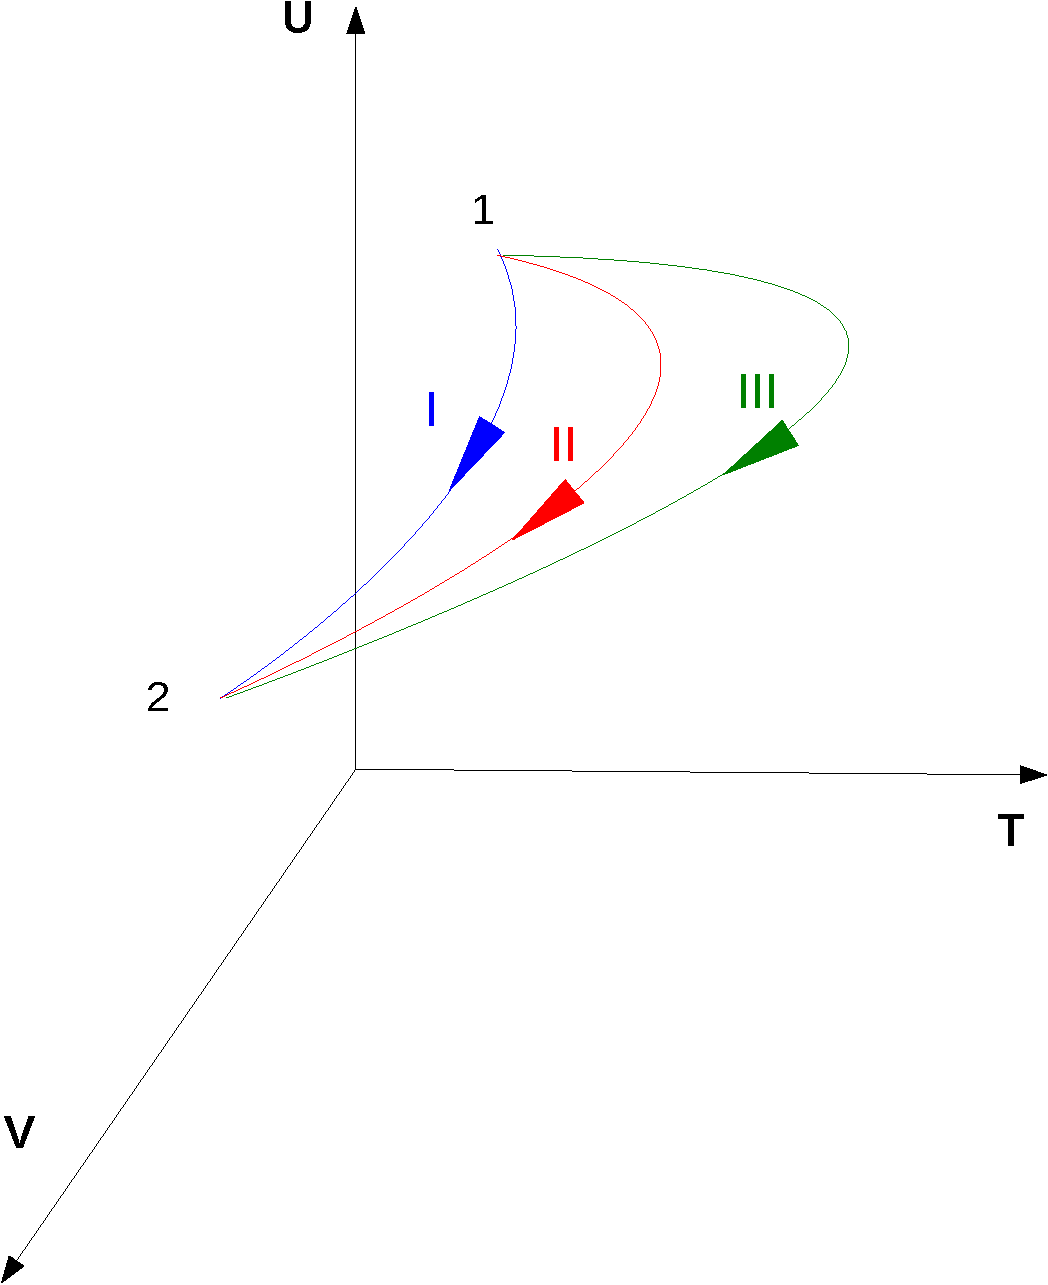
\includegraphics[width=9cm, height=9cm]{./Figs/Chp3_State-PathFunctions}
        \caption{State function: Change of internal function as a result of work and heat being exerted into the system by 3 distinct paths. Note that regardless the chosen path (from state 1 to state 2), $U_{1}$ and $U_{2}$ remain the same, although the amount of heat (represented here by changes in temperature, $T$) and work (\ie changes in volume, $V$) may vary significantly.}\label{Chapter:FirstLaw:Fig:StateFunctions}
     \end{center}
   \end{figure}
   
%%%
%%% SECTION
%%%
   \section{Reversible and Irreversible Processes}\label{Chapter:FirstLaw:Section:Reversibility}\index{Process!Reversible}\index{Process!Irreversible}
   Thermodynamic processes may change the state in two distinct ways:
   \begin{itemize}
     \item {\bf Reversible process} (also known as quasi-static process) is a process which can be stopped at any stage and reversed so that the system and the surroundings are exactly restored to their original states;
     \item {\bf Irreversible process} is a process in which heat is transferred through a finite temperature, thus it is not possible to return both the system and the surroundings to their original states.
   \end{itemize}
   Irreversibilities are of two types:
   \begin{itemize}
      \item {\it external irreversibilities} which are associated with dissipating effects outside the working fluid, \eg mechanical friction during a process due to some external force;
      \item {\it internal irreversibilities} which are associated with dissipating effects within the working fluid, \eg viscosity and inertial of a gas.
   \end{itemize}
   A set of definitions, characteristics and examples of these two processes are given by Table~\ref{Chapter:FirstLaw:TableDiffRevIrrev}. 
   
   
%%%
%%% SECTION
%%%
     \section{The First Law of Thermodynamics}\label{Chapter:FirstLaw:Section:FirstLaw}\index{Laws of Thermodynamics ! First law}
     \begin{subequations}
         Thermal energy is a macro-scale representation of micro-scale changes in mechanical energy (\ie work and heat). In a molecular scale, atoms and molecules are in random motion that can be associated with the kinetic energy of these `particles'. Tracking the motion and energy of each particle is addressed by a field of science called statistical (or quantum) thermodynamics; here we are interested in the consequences of the particles' motion, \ie oscillations in temperature as a measure of the average molecular-scale kinetic energy.
         \begin{shaded}
            \begin{center} {\bf Sign Notation}\end{center} 
              Before we proceed stating the {\it First Law}, we should define a sign notation used for all quantities in this document. Thus any form of energy:
              \begin{itemize}
                  \item Added to the system is assumed \blue{positive}, and;
                  \item Removed from the system is assumed \red{negative}.
              \end{itemize}
              Hence:
              \begin{itemize}
                 \renewcommand{\labelitemi}{$\star$}
                 \item heat added to the system by the neighbourhood is \blue{positive};
                 \item heat removed from the system to the neighbourhood is \red{negative};
                 \item work produced by the system and transferred to the neighbourhood is \red{negative};
                 \item work produced by the neighbourhood and transferred to the system is \blue{positive}.
              \end{itemize}
         \end{shaded}
         In most thermodynamic systems, changes in kinetic and potential energies are often assumed negligible\footnote{Here, we are assuming that such systems are not movable \wrt frames of reference.}, and Eqn.~\ref{Chapter:FirstLaw:Eqn:TotalEnergy3} becomes
            \begin{equation}
               \mfr[E]{2}{cv} - \mfr[E]{1}{cv} = U_{2}-U_{1} = Q_{1-2} + W_{1-2},\label{Chapter:FirstLaw:Eqn:FirstLaw1}
            \end{equation}
         in such cases, the internal energy of a system may be changed in any of the following ways: producing or receiving work and/or have heat being removed or added to the system. Heat and work are equivalent ways of changing the system's internal energy. It was experimentally observed that in isolated systems there is {\bf no} change in the internal energy.

         \begin{shaded}
            The {\it First Law of Thermodynamics} is effectively a statement of energy conservation: `the only way the energy of a closed system can be changed are through transfer of energy by work or heat' \citep{Moran_Book}. In other words: `the internal energy of an isolated system is constant' \citep{Atkins_Book}. Mathematically, these statements can be readily represented in differential form (\ie during infinitesimal changes in the state of the system) by,
            \begin{equation}
               d U = \delta Q + \delta W,\label{Chapter:FirstLaw:Eqn:FirstLaw2}
            \end{equation}
            
         \end{shaded}
   
     \end{subequations}

   %%%
   %%%
   \begin{landscape}
     \begin{table}
       \begin{tabular}{||l | l||}
         \hline\hline
             {\bf Reversible process} (RP)                                    &         {\bf Irreversible process}  (IP)                          \\
         \hline
             (a) RP can not be realised in practice;                          &  (a) All practical processes occurring are IP;                    \\
             (b) The process can be carried out in the reverse direction      &  (b) The process if carries out in reverse direction, it follows  \\
                 following the same path as followed in forward direction;    &      the path different from that in forward direction;           \\
             (c) A RP leaves no trace of occurrence of process upon the       &  (c) The evidences of process having occurred are evident even    \\
                 the system and surroundings after its reversal;              &      after reversal of IP;                                        \\
             (d) Such processes can occur in either directions without        &  (d) Occurrence of IPs in either directions is not possible, as   \\
                 violating the Second Law of Thermodynamics;                  &      in one direction it shall be accompanied with the violation  \\
                                                                              &      of the Second Law of Thermodynamics;                         \\
             (e) A system undergoing RPs has maximum efficiency. Therefore,   &  (e) Systems undergoing IPs do not have maximum efficiency as it  \\
                 sytems with RPs are considered as reference systems (\ie     &      accompanied by waste of energy;                              \\
                 benchmarks);                                                 &                                                                   \\
             (f) RPs occur at infinitesimal rate, \ie quasi-static process;   &  (f) IP occur at finite rate;                                     \\
             (g) System remains in thermodynamic equilibrium during occurrence&  (g) Systems does not remain in thermodynamic equilibrium during  \\
                 of such processes;                                           &      IPs;                                                         \\
         \hline
                                 {\bf Examples}                               &             {\bf Examples}                                        \\
             (h) Frictionless motion, controlled expansion and compression,   &   (h) Viscous fluid flow, inelastic deformation and hysteresis    \\
                 elastic deformations, polytropic expansion and compression   &       effects, free expansion, throttling processes, heat transfer\\
                 of fluids, electrolysis etc.                                 &       combustion, free expansion, diffusion etc.                  \\
         \hline\hline
       \end{tabular}
       \caption{Differences between reversible and irreversible processes \citep[extracted from][]{Singh_Book}.}
       \label{Chapter:FirstLaw:TableDiffRevIrrev}
     \end{table}
   \end{landscape}  
   
   % Example
   \begin{MyExample}{\begin{center}{\bf Example}\end{center}}
     \begin{example}\label{Chapter:FirstLaw:Example1}\citep{Atkins_Book}
        In a power station, the water pump is located in an isolated room. The electric motor of this pump produces 15 kJ of energy as mechanical work and loose 2 kJ of heat to the surroundings. Calculate the change in internal energy of the motor.  
     \end{example}

% SOLUTION
       \noindent{\bf Solution:}
       Here, the system is the electrical motor whereas the surroundings is the room. The work produced by the motor is $\delta W= -15$ kJ and the heat transferred from the engine to the room is $\delta Q = -2$ kJ, therefore 
          \begin{eqnarray}
             dU = \Delta U &=&  \delta Q + \delta W \nonumber \\
                &=& -15 -2 = -17\text{ kJ} \nonumber
          \end{eqnarray}
   \end{MyExample}

   % Example
   \begin{MyExample}{\begin{center}{\bf Example}\end{center}}
     \begin{example}\label{Chapter:FirstLaw:Example2}
       If $P_{1}$ = 3.00 atm, $V_{1}$ = 500 cm$^{3}$, $P_{2}$ = 1.00 atm and $V_{2}$ = 2000 cm$^{3}$. Calculate the work, $W_{\text{rev}}$ (in $J$), for the expansion processes shown in the following figure.
         \begin{center}
           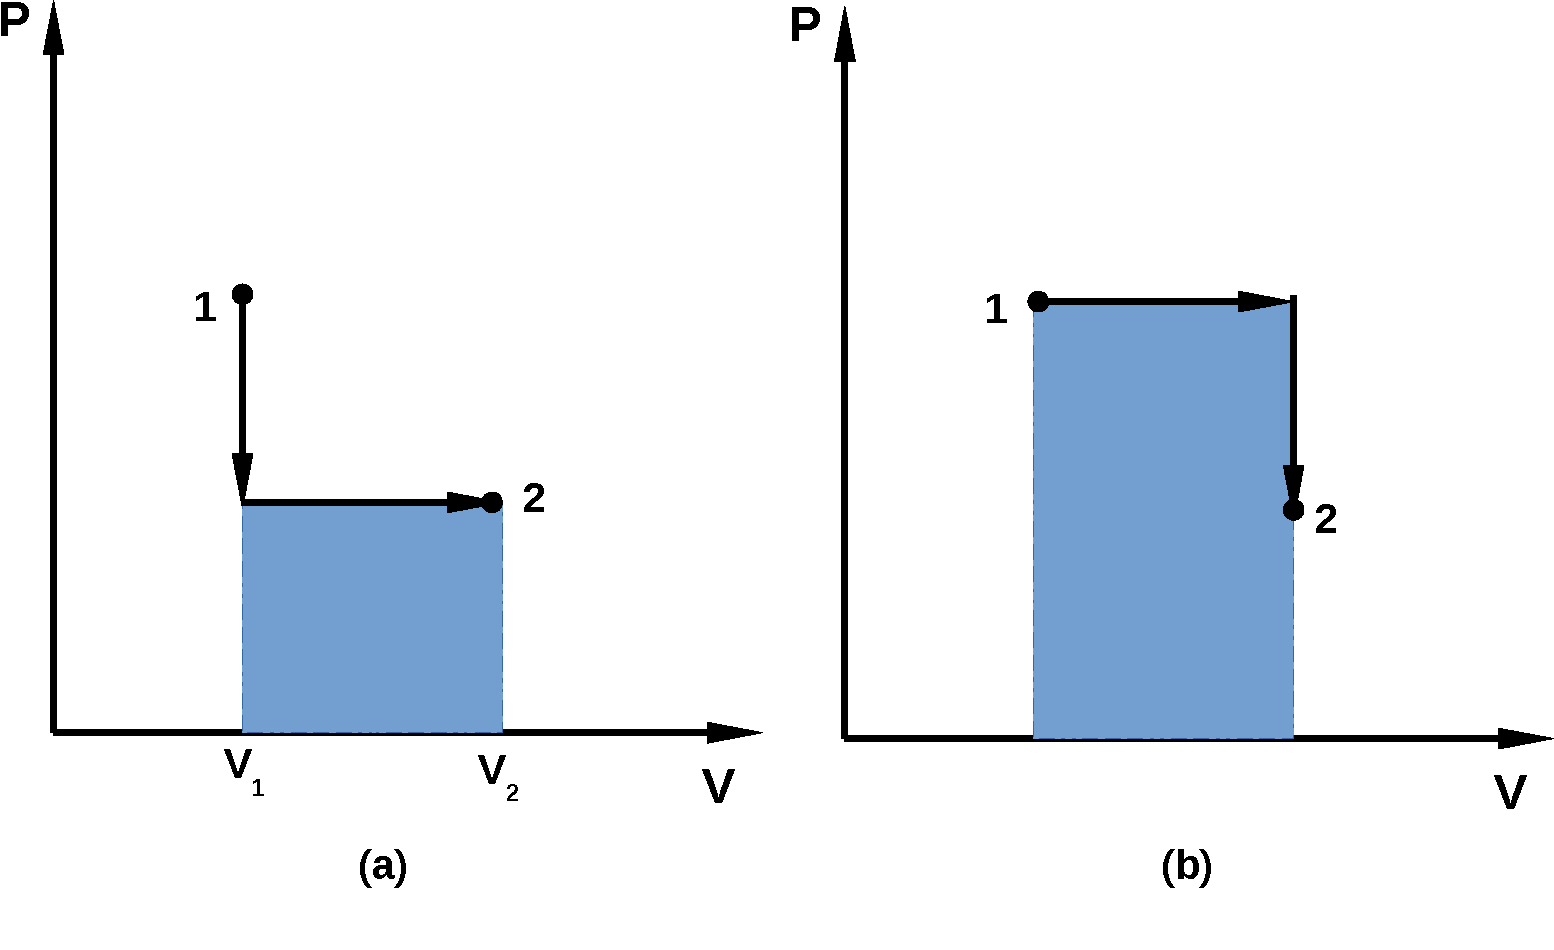
\includegraphics[width=.6\columnwidth,clip]{./Figs/Mod1Ex1}
         \end{center}
     \end{example}
     
% SOLUTION
       \noindent{\bf Solution:} $W_{\text{rev}}$ is related to the area below the curve. Thus, we should use the $PV$ work equation:
           \begin{itemize}
              \item For process {\bf (a)}: 
                 \begin{eqnarray}
                    d W = -PdV \Longrightarrow W &=& -P_{2}\left(V_{2}-V_{1}\right) \nonumber \\
                                                 &=& - 1\text{ atm}\left(2000-500\right)\text{ cm}^{3} = -1500\text{ atm.cm}^{3} \nonumber 
                 \end{eqnarray}
                 Now we need to convert {\it atm.cm}$^{3}$ to $J$, thus using the unit conversion table:
                 \begin{eqnarray}
                     W &=& -1500\blue{\cancel{\text{ atm}}}.\red{\cancel{\text{cm}^{3}}} \frc{1.01325\times 10^{5}\blue{\cancel{\text{ Pa}}}}{1\blue{\cancel{\text{ atm}}}} \frc{1 \frc{\text{kg}}{\text{m.s}^{2}}}{1\blue{\cancel{\text{ Pa}}}} \frc{1\text{ m}^{3}}{ 100^{3} \red{\cancel{\text{ cm}^{3}}}} \nonumber \\
                       &=& -151.9875 \blue{\cancel{\frc{\text{ kg.m}^{2}}{\text{s}^{2}}}} \frc{ 1 \text{ J}}{ \blue{\cancel{\frc{\text{ kg.m}^{2}}{\text{s}^{2}}}}} \nonumber\\
                       &=& -151.9875\text{ J} \nonumber
                 \end{eqnarray}
%
              \item For process {\bf (b)}, since $P$ is constant, i.e., $P_{1}=P_{2}$:
                 \begin{eqnarray}
                    d W = -PdV \Longrightarrow W &=& -P_{1}\left(V_{2}-V_{1}\right) \nonumber \\
                                                 &=& - 3\text{ atm}\left(2000-500\right)\text{ cm}^{3} = -4500\text{ atm.cm}^{3} \nonumber \\
                                                 &=& -455.9625\text{ J} \nonumber
                 \end{eqnarray}
           \end{itemize}
   \end{MyExample}

%%%
%%% SECTION
%%%
     \section{Cycles: Representation of the First Law}\label{Chapter:FirstLaw:Section:FirstLaw_Cycle}\index{Laws of Thermodynamics ! First law}\index{Cycles}
        \begin{subequations}
           \begin{shaded}
               During any cycle, the cyclic integral of heat added to a system is proportional to the cyclic integral of work done by the system.
           \end{shaded}
           This statement clearly indicates that during a cycle the internal energy is zero, $\left(\Delta U\right)_{\text{cycle}}=0$. The mathematical representation of the first law in a cycle is
             \begin{equation}
               \displaystyle\oint \delta Q = -\displaystyle\oint \delta W,\label{Chapter:FirstLaw:Eqn:FirstLawCycle}
             \end{equation}
             where line integral $\left(\oint\right)$ is defined in Appendix~\ref{Appendix_Calculus:Section:LineIntegral}. Two main practical systems arise from the application of the first law to the definition of cycles (Section~\ref{Chapter:Introduction:Section:Introduction:ProcessesCyclesDefinition}): power and refrigeration cycles.
      
%%%% SUBSECTION
          \subsection{Power Cycles}\index{Cycles! Power }
             Power cycles (Fig.~\ref{Chapter:FirstLaw:Fig:PowerRefrigSystems}a) are systems that deliver a net work transfer of energy to the surroundings during each cycle, where
               \begin{displaymath}
                  W_{cycle} = Q_{in} - Q_{out},\;\;\;\text{ with }\;\;\; Q_{in} > Q_{out}.
               \end{displaymath}
             The energy supplied by heat transfer to a system on a power cycle is often derived from combustion processes. Such cycles are used to quantitatively describe the work produced in power plants, and are often assessed through the thermal efficiency of the process,\index{Cycles! Power! Thermal efficiency }
       \begin{equation}
           \eta =\frc{W_{cycle}}{Q_{in}} = \frc{Q_{in} - Q_{out}}{Q_{in}} = 1 - \frc{Q_{out}}{Q_{in}} < 1.\label{Chapter:FirstLaw:Eqn:FirstLawCycle:PowerEfficiency}
       \end{equation}
       For reversible power cycles the ratio of heat transfer, $Q_{cold}/Q_{hot}$ depends only on the reservoirs' temperatures and can be simplified to
       \begin{equation}
          \frc{Q_{\text{cold}}}{Q_{\text{hot}}} =  \frc{T_{\text{cold}}}{T_{\text{hot}}}.\label{Chapter:FirstLaw:Eqn:FirstLawCycle:PowerEfficiency2}
       \end{equation}
       One of the conditions for this expression to be valid is $T_{\text{hot}}\ne0$, indeed {\bf reservoir temperature are always assumed as absolute temperature, \ie expressed in Kelvin}.
       \begin{shaded}
           Thus the thermal efficiency of a reversible power cycle while operating between thermal reservoirs at temperatures $T_{hot}$ and $T_{cold}$ is expressed as
          \begin{equation}
            \eta_{\text{max}} = 1 - \frc{T_{\text{cold}}}{T_{\text{hot}}}\label{Chapter:FirstLaw:Eqn:FirstLawCycle:PowerCarnotEfficiency}
          \end{equation}
          $\eta_{\text{max}}$ is also known as the {\it Carnot efficiency}\index{Carnot Efficiency} and it is the maximum efficiency any power cycle can have while operating between the 2 reservoirs.
       \end{shaded}

   \begin{figure}[h]
      \vbox{
        \hbox{ \hspace{-1.5cm}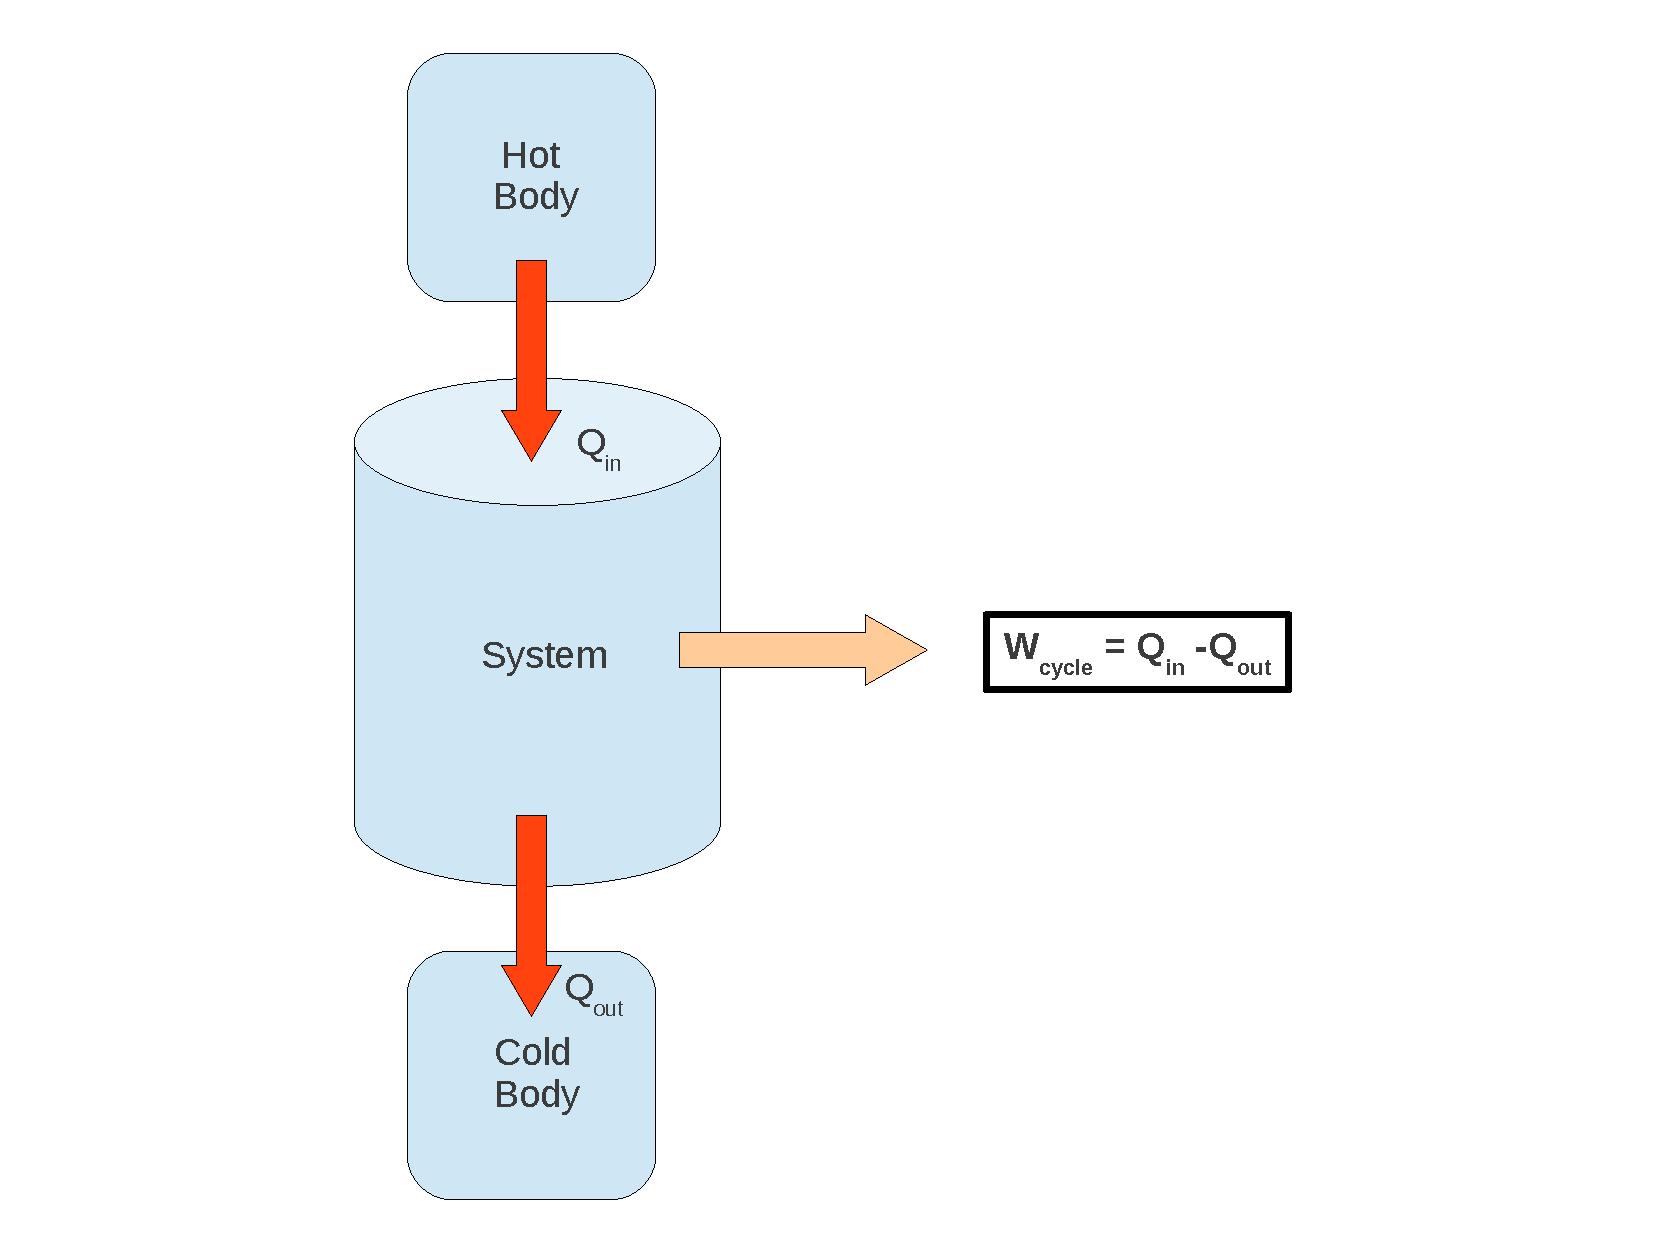
\includegraphics[width=.7\columnwidth,clip]{./Figs/FirstLaw_Cycle_01}
               \hspace{-2.5cm}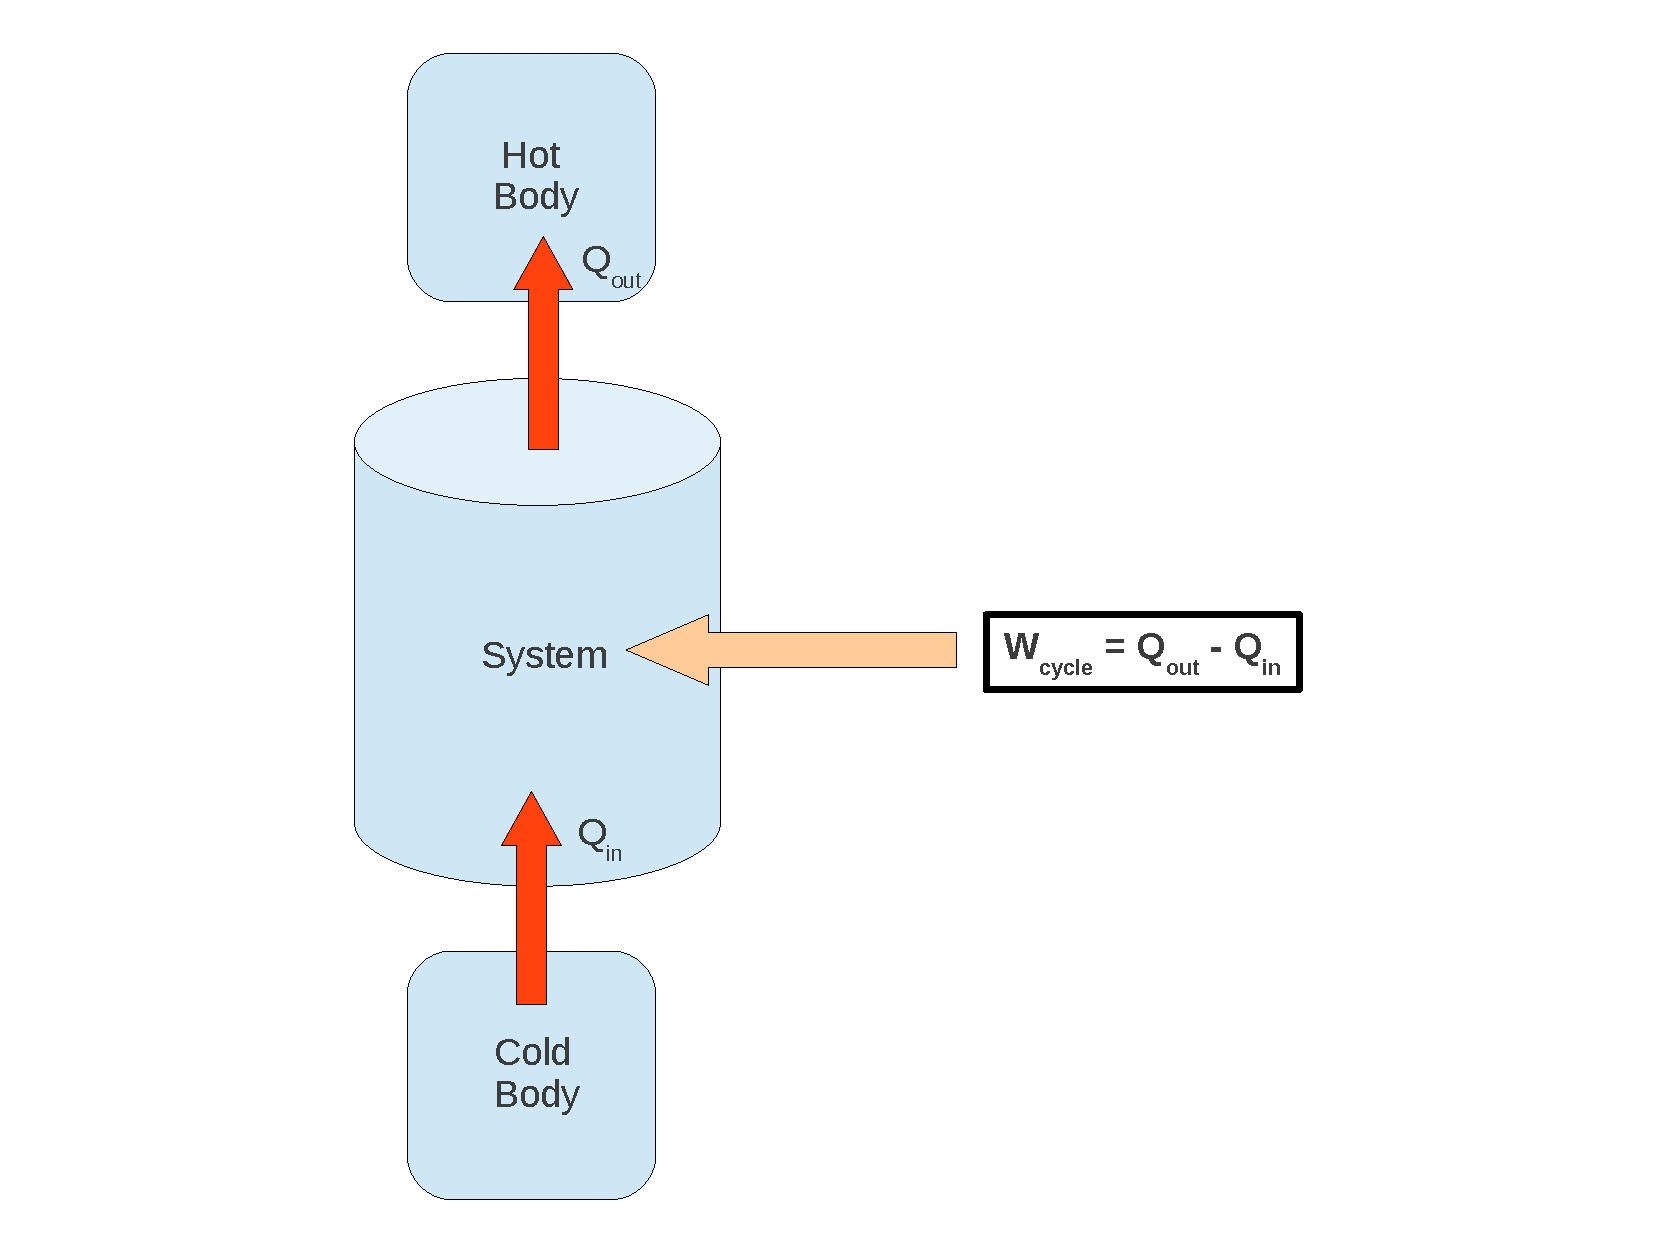
\includegraphics[width=.7\columnwidth,clip]{./Figs/FirstLaw_Cycle_02}}
        \vspace{-0.cm}
        \hbox{\hspace{4cm}(a)\hspace{7cm}(b)}}
       \caption{Schematic representation of (a) power and (b) refrigeration cycles.}\label{Chapter:FirstLaw:Fig:PowerRefrigSystems}
   \end{figure}    

%%%% SUBSECTION
          \subsection{Refrigeration Cycles}\index{Cycles! Refrigeration }
           Refrigeration cycles (Fig.~\ref{Chapter:FirstLaw:Fig:PowerRefrigSystems}b) are systems in which Q$_{in}$ is associated with the heat energy transferred into the system from the cold body. Q$_{out}$ is the energy discharged via heat transfer from the system to the hot body, 
           \begin{displaymath}
              W_{cycle} = Q_{out} - Q_{in}.
           \end{displaymath}
            \begin{shaded}
               The aim of such cycles is to cool a refrigerated body or to maintain the temperature of a body bellow that of the surrounding. Refrigeration cycles are assessed through the coefficient of performance (COP)\index{Cycles!Refrigeration ! Coefficient of performance },
                 \begin{equation}
                   \beta = \frc{Q_{in}}{W_{cycle}} = \frc{Q_{in}}{Q_{out} - Q_{in}}.\label{Chapter:FirstLaw:Eqn:FirstLawCycle:COP}
                 \end{equation}
          \end{shaded}
        \end{subequations}
   

%%%
%%% SECTION
%%%
     \section{Enthalpy}\label{Chapter:FirstLaw:Section:Enthalpy}\index{Enthalpy}
        \begin{subequations}
          Let's consider a gas contained in a piston-cylinder system undergoing a quasi-static isobaric process. Let's also assume that there are no changes in kinetic and potential energies and that the only work done during the process is the one associated with the piston's movement. The first law stated that the internal energy is a result of changes in work and heat,
          \begin{displaymath}
            dU = \delta Q + \delta W,\;\;\;\text{ and } \;\;\; \delta W = -\int\limits_{1}^{2} PdV = -P\left(V_{2}-V_{1}\right).
          \end{displaymath}
          \begin{shaded}
             Replacing the work into the first law equation
             \begin{eqnarray}
                \delta Q &=& dU - \delta W = U_{2} - U_{1} + P_{2}V_{2} - P_{1}V_{1}\nonumber \\
                         &=& \left(U_{2}+P_{2}V_{2}\right) - \left(U_{1}+P_{1}V_{1}\right).\label{Chapter:FirstLaw:Eqn:EnthalpyDefinition1}
             \end{eqnarray}
             The terms in brackets, $U+PV$, are thermodynamic properties that depend only on the state of the system and, as such, define a new extensive property, the {\it enthalpy},
             \begin{equation}
               H\equiv U + PV.\label{Chapter:FirstLaw:Eqn:EnthalpyDefinition2}
             \end{equation}
             Replacing Eqn.~\ref{Chapter:FirstLaw:Eqn:EnthalpyDefinition1} in \ref{Chapter:FirstLaw:Eqn:EnthalpyDefinition2}
             \begin{equation}
               \delta Q = \overbrace{\left(U_{2}+P_{2}V_{2}\right)}^{H_{2}} - \overbrace{\left(U_{1}+P_{1}V_{1}\right)}^{H_{1}} = H_{2}-H_{1} = \Delta H,\label{Chapter:FirstLaw:Eqn:EnthalpyDefinition3}
             \end{equation}
             \ie the {\it change in enthalpy leads to the heat transfer for isobaric processes}. 
          \end{shaded}
       
        \end{subequations}

%%%
%%% SECTION
%%%
    \section{Heat Capacities}\label{Chapter:FirstLaw:Section:HeatCapacity}
      \begin{subequations}

        %%% Subsection
        \subsection{Constant Volume and Constant Pressure Heat Capacities}\index{Heat Capacity ! Constant Volume}\index{Heat Capacity ! Constant Pressure}\index{$C_{v}$| see{ Heat Capacity}}\index{$C_{p}$| see{ Heat Capacity}}
            {\it Specific heat capacity} can be defined as the amount of heat necessary to increase the temperature of a unit mass of material by one degree. Mathematically, it can be defined as
            \begin{displaymath}
              C\equiv \frc{1}{m}\frc{\delta Q}{\delta T}.
            \end{displaymath}
            As $Q$ is path-dependent, $C$ also is, and from the first law
            \begin{displaymath}
              \delta Q = dU - \delta W \;\;\Longrightarrow\;\; dU + PdV,
            \end{displaymath}
            two properties can be defined depending upon the path:
            \begin{enumerate}[(i)]
              \item Constant volume: in which the term $PdV$ vanishes and the specific heat at constant volume $\left(C_{v}\right)$ is
                \begin{equation}
                  C_{v} = \frc{1}{m}\left(\frc{\delta Q}{\delta T}\right)_{V} = \frc{1}{m}\left(\frc{\partial U}{\partial T}\right)_{V} = \left(\frc{\partial u}{\partial T}\right)_{V}\label{Chapter:FirstLaw:Eqn:HeatCapacityConstVolume1}
                \end{equation}
              \item Constant pressure: in which the work term can be integrated at constant pressure, hence the heat transfer can be expressed in terms of the enthalpy change (Eqn.~\ref{Chapter:FirstLaw:Eqn:EnthalpyDefinition3}),
                \begin{equation}
                  C_{p} = \frc{1}{m}\left(\frc{\delta Q}{\delta T}\right)_{P} = \frc{1}{m}\left(\frc{\partial H}{\partial T}\right)_{P} = \left(\frc{\partial h}{\partial T}\right)_{P}\label{Chapter:FirstLaw:Eqn:HeatCapacityConstPressure1}
                \end{equation}
            \end{enumerate}
            $C_{p}\left(T,P\right)$ and $C_{v}\left(T,v\right)$ are thermodynamic properties for general materials and can vary with the independent variables $\left(T, P, v\right)$. Here, $h$ and $u$ are specific enthalpy and internal energy with units J.kg$^{-1}$.
            
        %%% Subsection
        \subsection{Heat Capacity Relations for Ideal Gases}\label{Chapter:FirstLaw:Section:HeatCapacity:IdealGas}
          For ideal gases, one can use the fundamental thermodynamic relation that defined enthalpy (Eqn.~\ref{Chapter:FirstLaw:Eqn:EnthalpyDefinition2}) and the ideal gas EOS, $Pv=RT$ (Eqn.~\ref{Chapter:Intro_Property_of_Gases:Eqn:IdealEOS}), to redefine the specific enthalpy
          \begin{equation}
            h = u(T) + RT,\label{Chapter:FirstLaw:Eqn:EnthalpyDefinition4}
          \end{equation}
          of an ideal gas as a function of $T$ only, \ie $h=h(T)$.  The specific heat of an ideal gas at contant volume is expressed as
          \begin{displaymath}
             C_{v}(T,v) = \left(\frc{\partial u}{\partial T}\right)_{v} = \frc{d}{dT}\left(u(T)\right) = C_{v}(T).
          \end{displaymath}
          In other words, $C_{v}$ is property that can be expressed as function of $T$ and $v$ (thus being defined as a partial differential equation with the differential operator $\partial$), however if a process is assumed isochoric (\ie constant volume) this property becomes a function of only the temperature (and therefore defined as an ordinary differential equation with the differential operator $d$),
                \begin{equation}
                  du = C_{v}(T)dT.\label{Chapter:FirstLaw:Eqn:HeatCapacityConstVolume2}
                \end{equation}
          A similar argument can be used for $C_{p}$ in isobaric processes, leading to
                \begin{equation}
                  dh = C_{p}(T)dT.\label{Chapter:FirstLaw:Eqn:HeatCapacityConstPressure2}
                \end{equation}
          \begin{shaded}
             Differentiating Eqn.~\ref{Chapter:FirstLaw:Eqn:EnthalpyDefinition4} and replacing $du$ and $dh$,
                \begin{eqnarray}
                   && dh = du + RdT \nonumber \\
                   && C_{p}(T)dT = C_{v}(T)dT + RdT \;\;\;\Longrightarrow C_{p}(T) = C_{v} + R \nonumber \\
                   && C_{p}(T) - C_{v}(T) = R.\label{Chapter:FirstLaw:Eqn:HeatCapacitiesRelation_IdealGas1}
                \end{eqnarray}
             A useful relationship in engineering thermodynamics is the ratio of specific heats (or isentropic index),
                \begin{equation}
                  \gamma = \frc{C_{p}}{C_{v}},\label{Chapter:FirstLaw:Eqn:HeatCapacitiesRelation1}
                \end{equation}
             which is valid for any material. For an ideal gas, this relation reduces to 
                \begin{equation}
                  \gamma = \frc{C_{v}(T)+R}{C_{v}(T)} = 1 + \frc{R}{C_{v}(T)}.\label{Chapter:FirstLaw:Eqn:HeatCapacitiesRelation_IdealGas2}
                \end{equation}
             Other heat capacity based relations for ideal gases can be obtained from Eqns.~\ref{Chapter:FirstLaw:Eqn:FirstLaw2}, \ref{Chapter:FirstLaw:Eqn:EnthalpyDefinition2} and \ref{Chapter:Intro_Property_of_Gases:Eqn:IdealEOS}:
                \begin{equation}
                   \delta Q = 
                      \begin{cases}
                         C_{p}dT - \frc{RT}{P}dP, \label{Chapter:FirstLaw:Eqn:HeatCapacitiesRelation_IdealGas3} \\
                         \frc{C_{p}}{R}PdV + \frc{C_{v}}{R}VdP.
                      \end{cases}
                \end{equation}
                These relations, although apparently simple, reveal the dependence of heat transfer on temperature, pressure and volume in processes involving ideal gases.
          \end{shaded}


        \end{subequations}


   % Example
   \begin{MyExample}{\begin{center}{\bf Example}\end{center}}
     \begin{example}\label{Chapter:FirstLaw:Example3}
       Calculate the internal energy (in $J$) when 1 mol of water is isobarically heated from 25$^{\circ}$C to 30$^{\circ}$C at 1 atm. Given: densities of water are 0.9970 g.cm$^{-3}$ at 0$^{\circ}$C and 0.9956 g.cm$^{-3}$ at 100$^{\circ}$C. Molar mass and heat capacity at constant pressure of water are 18 g.mol$^{-1}$ and 1 cal.$\left(\text{g.}^{\circ}\text{C}\right)^{-1}$, respectively.
     \end{example}
     
% SOLUTION
       \noindent{\bf Solution:} From the 1$^{\text{st}}$ Law, $U=Q+W$ ,and in order to calculate $U$ we first need to obtain heat ($Q$) and work ($W$). $Q$ can be obtained from the heat capacity equation
          \begin{displaymath}
             Q = m C_{p} \Delta T,
          \end{displaymath}  
          where $m$ is the mass of water can be obtained from
          \begin{displaymath}
             n = \frc{m}{MW} \Longrightarrow  m = n.MW = 1\text{ mol} . 18 \frc{\text{g}}{\text{mol}} = 18 \text{ g}
          \end{displaymath}
          $n$ and $MW$ are number of moles and molar mass, respectively. Now,
          \begin{displaymath}
             Q = m C_{p} \Delta T = 18\text{ g} . 1 \frc{\text{ cal}}{\text{g.}^{\circ}\text{C}}.\left(30-25\right)^{\circ}\text{C} = 90\text{ cal}
          \end{displaymath}  
          Now, we should calculate the work through $W=-P\Delta V$, however $V$ is not known, but we can obtain it from the density relation $V=m/\rho$, thus
          \begin{displaymath}
             W = - P\Delta V = -P\left(V_{2}-V_{1}\right) = -P\left(\frc{m}{\rho_{2}} - \frc{m}{\rho_{1}}\right) = -0.025\text{atm.cm}^{3} = -0.0006\text{ cal} 
          \end{displaymath}
          Now, calculating the internal energy,
          \begin{displaymath}
             U = Q + W = 89.9994\cancel{\text{ cal}} . \frc{ 4.186\text{ J}}{1\cancel{\text{ cal}}} = 376.7375 \text{ J}
          \end{displaymath}
   \end{MyExample}


   % Example
   \begin{MyExample}{\begin{center}{\bf Example}\end{center}}
     \begin{example}\label{Chapter:FirstLaw:Example4}\citep{Rajput_Book}
       A 0.3 m$^{3}$  tank contains oxygen initially at 100 kPa and 300 K. A paddle wheel within the tank is rotated until the pressure inside rise to 150 kPa. During the process 2 kJ of heat is lost to the surroundings. Determine the paddle-wheel work done (in kJ). Neglect the energy stored in the paddle wheel and assume the heat capacity at constant volume of oxygen is 0.6745 kJ.$\left(\text{kg.K}\right)^{1}$. Given molar mass of oxygen of 32 g.mol$^{-1}$.
     \end{example}
     
% SOLUTION
       \noindent{\bf Solution:} The volume of the tank remains constant $V_{2}=V_{1}=V=$ 0.3 m$^{3}$ during the whole process. Thus, we can define:
            \begin{center}
              \begin{tabular}{l l l l}
                 Initial Condition & $P_{1}=$ 100 kPa   & $T_{1}=$ 300 K         & $V_{1}=$ 0.3 m$^{3}$  \\
                 Final Condition   & $P_{2}=$ 150 kPa   &                       & $V_{2}=$ 0.3 m$^{3}$ \\
                 Heat Loss         & $Q=$ -2 kJ        &                       &                    
              \end{tabular}
            \end{center}
       The compression occurs in a closed system (i.e., constant mass) and, as there is no further information, we may consider that oxygen behaves as an ideal gas. The work added to the system by the paddle can be expressed by $U=Q+W$. Our first step is to calculate $T_{2}$,
       \begin{displaymath}
          \frc{P V}{T} = \text{ constant} \Rightarrow \frc{P_{1}V_{1}}{T_{1}} = \frc{P_{2}V_{2}}{T_{2}} \Rightarrow \frc{P_{1}}{T_{1}}=\frc{P_{2}}{T_{2}} \Rightarrow T_{2} = 450\text{ K}
       \end{displaymath}
        The specific internal energy can defined by the fundamental relation, $du=C_{v}dT$ (check the units for this relation!), where $C_{v}$ is the heat capacity at constant volume thus,
       \begin{displaymath}
          \Delta U = m\Delta u = C_{v}\Delta T = Q + W,
       \end{displaymath}
       therefore, we need to obtain the mass of oxygen in the tank through the ideal gas equation of state,
       \begin{eqnarray}
         P V = n R T \Rightarrow n = \frc{m}{MW} = \frc{P V}{R T} \Rightarrow m &=& \frc{ MW P V}{R T} \nonumber \\
                                                      &=& \frc{ 32\frc{\text{ g}}{\text{mol}} 100\text{ kPa} . 0.3\text{ m}^{3}}{ 8.3143 \frc{\text{J}}{\text{mol.K}} 300\text{ K}} \nonumber \\
                                                      &=& 0.3848 \frc{\text{ g.kPa.m}^{3}}{\text{J}} \frc{1 \text{ J}}{1\text{ N.m}} \frc{1000 \text{ Pa}}{1 \text{ kPa}} \frc{ 1 \text{ N.m}^{-2}}{1\text{ Pa}} \nonumber\\
                                                      &=& 0.3848\text{ kg}\nonumber
       \end{eqnarray}
       Thus
       \begin{eqnarray}
          \Delta u = m C_{v}\Delta T = Q + W \Rightarrow W &=& m C_{v}\left(T_{2}-T_{1}\right) - Q \nonumber \\
                                                          &=& 0.3848\text{ kg} \times 0.6745 \frc{\text{kJ}}{\text{kg.K}}\times (450-300)\text{ K} - (-2 \text{ kJ}) \nonumber \\
                                                          &=& 40.9321\text{ kJ}. \nonumber
       \end{eqnarray}
       The paddle-wheel executed 40.9321 kJ of work to the system.
   \end{MyExample}
   
   % Example
   \begin{MyExample}{\begin{center}{\bf Example}\end{center}}
     \begin{example}\label{Chapter:FirstLaw:Example4}\citep{Atkins_Book}
       Calculate the change in molar enthalpy of N $_{2}$(g) when it is heated from 25$^{\circ}$C to 100$^{\circ}$C. The heat capacity is given by
       \begin{displaymath}
         C_{p} = a + bT + \frc{c}{T^{2}}, 
       \end{displaymath}
       where $\left[C_{p}\right]=$ J.mol$^{-1}$.K$^{-1}$, $\left[T\right]=$ K, $a=$ = 28.58 J.mol$^{-1}$.K$^{-1}$, $b=$ 3.77$\times$10$^{-3}$ J.mol$^{-1}$ and $c=$ -0.50$\times$10$^{5}$ J.mol$^{-1}$.K. Given molar enthalpy of N $_{2}$(g) at 25$^{\circ}$C is 29.1400 J.mol$^{-1}$.
     \end{example}
     
% SOLUTION
     \noindent{\bf Solution:} As all units contain temperature in Kelvin, let's first convert them as $T_{1}=$ 298.15 K and $T_{2}=$ 373.15 K. Now, we need to calculate the change in molar enthalpy in this temperature range using the definition of heat capacity,
        \begin{eqnarray}
          && C_{p} = \left(\frc{\partial H}{\partial T}\right)_{P} \;\;\Longrightarrow\;\; dH = C_{p}dT \nonumber \\
          && \int\limits_{H_{1}\left(T_{1}\right)}^{H_{2}\left(T_{2}\right)}dH = \int\limits_{T_{1}}^{T_{2}} C_{p}dT = \int\limits_{T_{1}}^{T_{2}} \left(a + bT + \frc{c}{T^{2}}\right)dT \nonumber \\
          && H_{2}\left(T_{2}\right) - H_{1}\left(T_{1}\right) = a\left(T_{2}-T_{1}\right) + \frc{1}{2}b\left(T_{2}^{2}-T_{1}^{2}\right) - c\left(\frc{1}{T_{2}}-\frc{1}{T_{1}}\right) \nonumber 
        \end{eqnarray}
        Solving this expression with the constants and $H_{1}\left(T_{1}\right)=H\left(\text{298.15 K}\right)=$ 29.14 J.mol$^{-1}$, leads to $H_{2}\left(T_{2}\right) = H\left(\text{373.15 K}\right)=$ 2238.4047 J.mol$^{-1}$. Thus, change in molar enthalpy, \ie $H_{2}\left(T_{2}\right) - H_{1}\left(T_{1}\right)$,  of N $_{2}$(g) is 2209.2647 J.mol$^{-1}$.

   \end{MyExample} 
       
      
%%%
%%% SECTION
%%%
     \section{Work Done at Moving Boundary}\label{Chapter:FirstLaw:Section:Work}
     \begin{subequations}
        In Section~\ref{Chapter:Introduction:Section:ThermodynamicWorkHeat}, the work produced by (or exerted on) the system was defined by Eqn.~\ref{Chpt01_Work2},
           \begin{equation}
              dW = -PdV \;\;\Longrightarrow \;\; W = - \int\limits_{V_{1}}^{V_{2}} PdV,\label{Chapter:FirstLaw:Eqn:Work1}
           \end{equation}
        where $P$ is the pressure and $V$ is the variable volume. Let's consider a system comprising a cylinder containing a compressible gas $\left(\text{with }V_{1}\text{ and } P_{g} = P_{1}\right)$ with a movable piston (Fig.~\ref{Chapter:FirstLaw:Fig:Work1}). An external pressure $\left(P_{\text{ext}} > P_{1}\right)$ is imposed on the piston and continuously compress the gas until the pressures are equalised $\left(P_{\text{ext}} = P_{g} = P_{2}\right)$. At the end of such compression (\ie at state 2) $V_{2}<V_{1}$ and the work $W$ is positive, \ie energy is transferred to the system through the application of an external force. Now, let's assume that at state 2, $P_{\text{ext}}$ is replaced by a new pressure, $P^{\star}_{\text{ext}}=P_{1}$, such that $P^{\star}_{\text{ext}} < P_{\text{ext}} \left(= P_{g} = P_{2}\right)$. As the new pressure is smaller than the pressure inside the cylinder $\left(P_{2}\right)$, the gas will expand until the external and internal pressure are equal, \ie $P_{g} = P^{\star}_{\text{ext}} = P_{1}$. At the end of such expansion from $V_{2}$ to $V_{1}$, the work
           \begin{displaymath}
              W = - \int\limits_{V_{2}}^{V_{1}} PdV,
           \end{displaymath}
           is negative, \ie energy is transferred from the system to the neighbourhood. In these expansion and compression processes, two scenarios may occur: constant or variable pressures. Equation~\ref{Chapter:FirstLaw:Eqn:Work1} is solved according with these scenarios.
\medskip
% Figure
   \begin{figure}[h]
     \begin{center}
        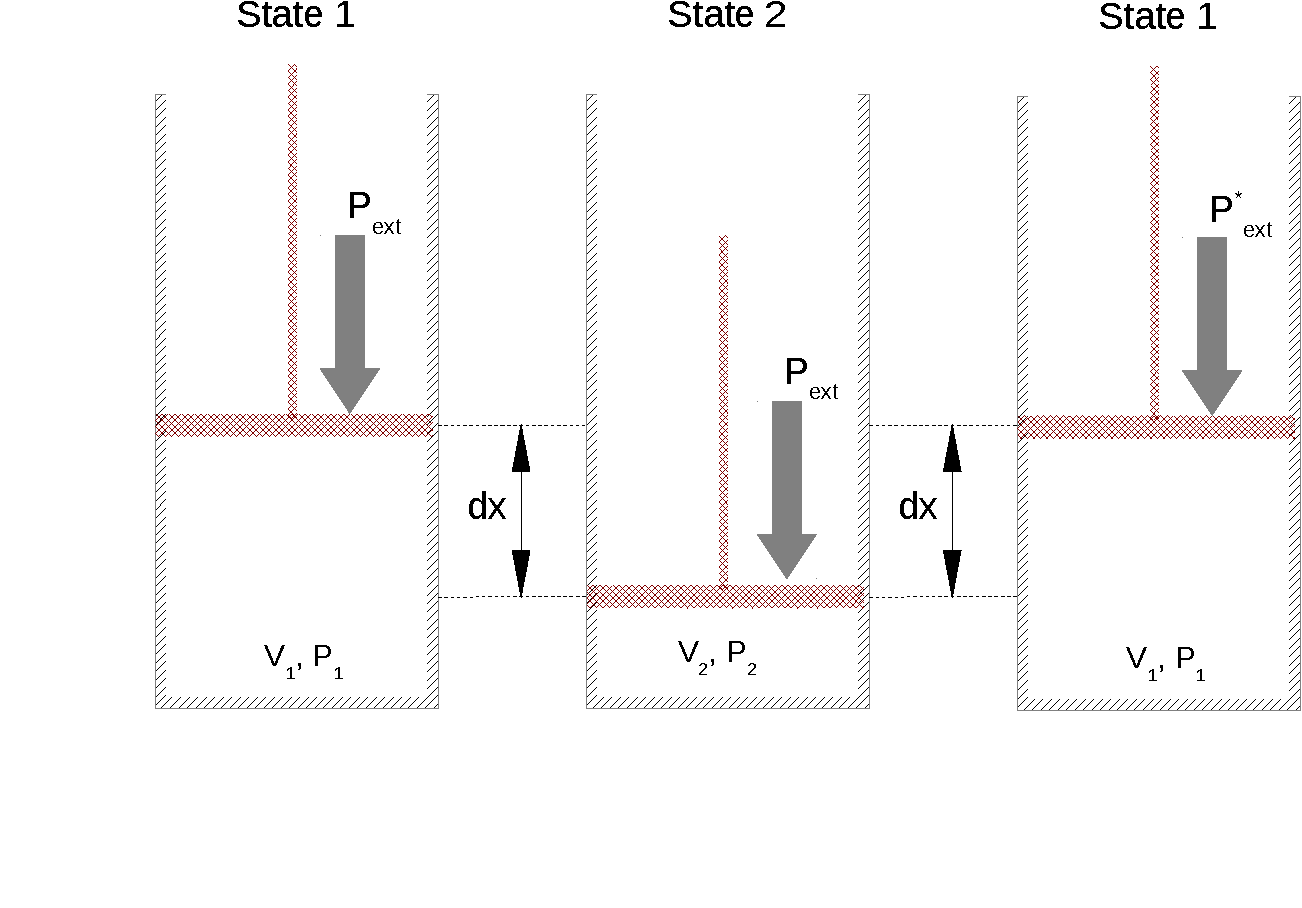
\includegraphics[width=0.7\columnwidth,clip]{./Figs/Chp3_PistonCylinder1}\vspace{-2cm}
        \caption{Compression and expansion of a piston as a result of an external force.}\label{Chapter:FirstLaw:Fig:Work1}
     \end{center}
   \end{figure}
\medskip


%%%
%%% SECTION
%%%
     \subsection{Expansion/Compression under Constant Pressure}\label{Chapter:FirstLaw:Section:Work_ConstantPressure}
        If the external pressure $P=P_{\text{ext}}$ is constant, the integral (Eqn.~\ref{Chapter:FirstLaw:Eqn:Work1}) can be readily solved with the initial and final volumes,
           \begin{shaded}
             \begin{equation}
                dW = -PdV \;\;\Longrightarrow \;\; W = - P\int\limits_{V_{1}}^{V_{2}} dV = - P\left(V_{2}-V_{1}\right) = -P\Delta V.\label{Chapter:FirstLaw:Eqn:Work_ConstPressure}
             \end{equation}
           \end{shaded}
           This integral can be graphically illustrated by the area under the $PV$ curve of Fig.~\ref{Chapter:FirstLaw:Fig:Work2}a. The work is equal to area beneath the horizontal line at $P=P_{\text{ext}}$ lying between $V_{1}$ and $V_{2}$.
           
% Figure
\begin{figure}[h]
  \vbox{
     \hbox{\hspace{2cm}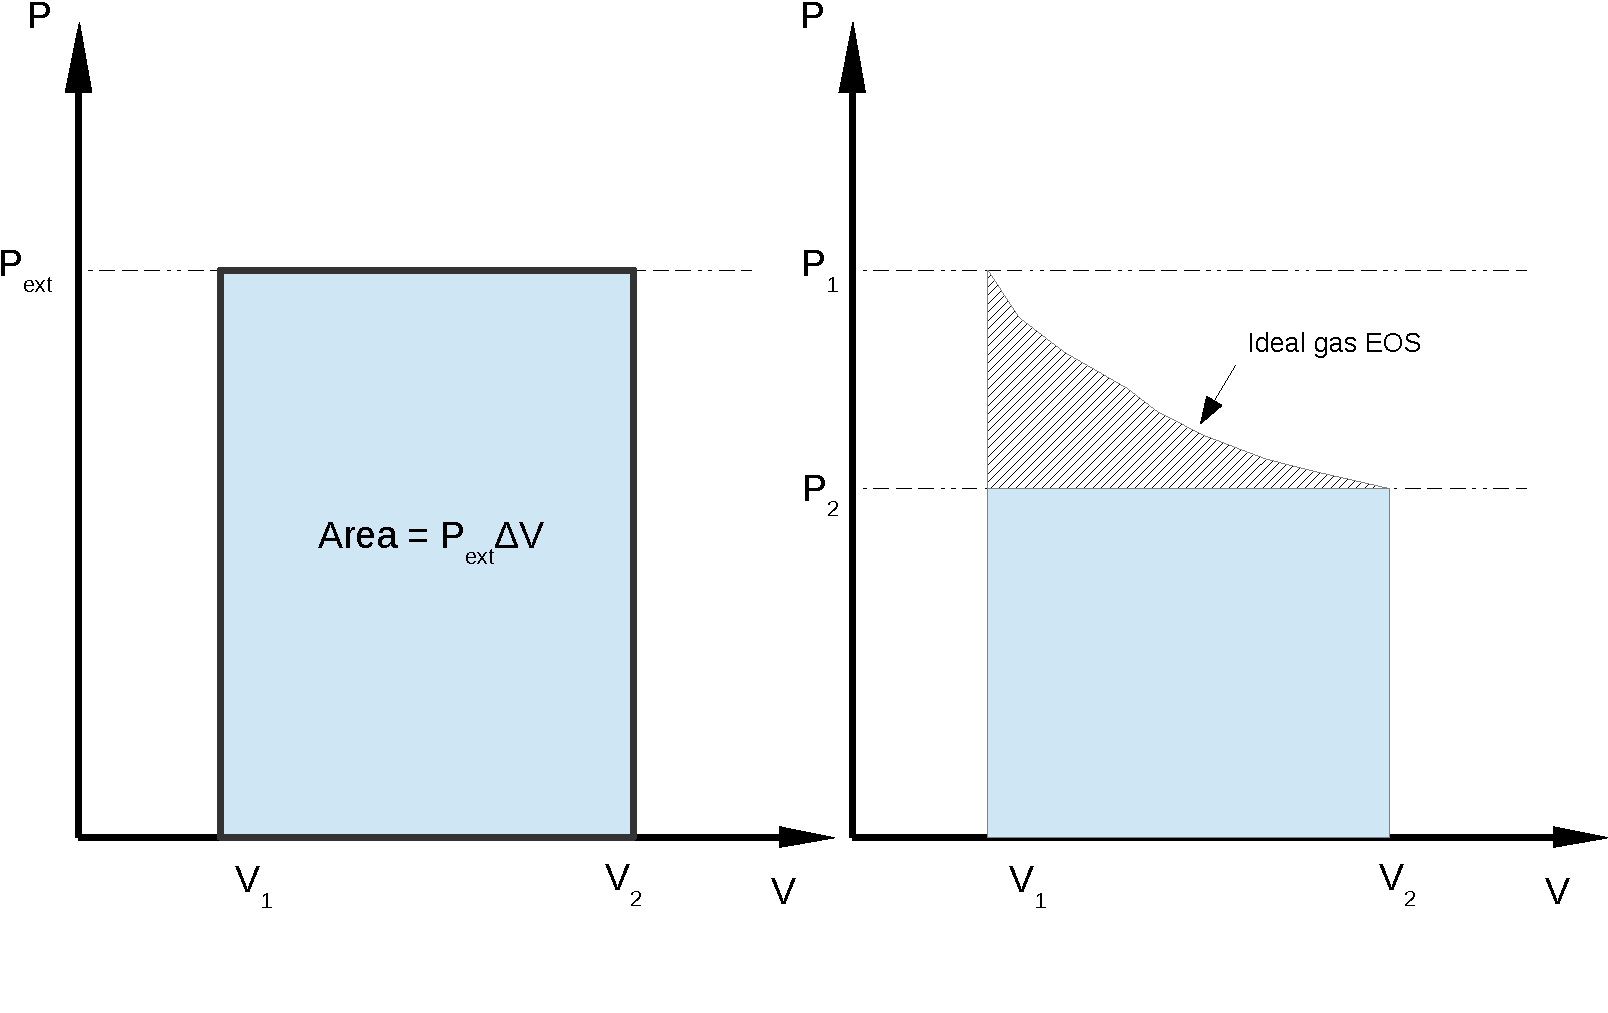
\includegraphics[width=0.7\columnwidth,clip]{./Figs/Chp3_PistonCylinder2}}
     \vspace{-1.cm}
     \hbox{\hspace{5cm}(a)\hspace{4.5cm}(b)}}%\vspace{-0.cm}
        \caption{Ideal gas expansion under isothermal conditions: (a) irreversible work at constant external pressure is equal to the blue area (Eqn.~\ref{Chapter:FirstLaw:Eqn:Work_ConstPressure}); (b) reversible work from $V_{1}$ to $V_{2}$ is given by the area below the curve (\ie blue and hatched areas).}\label{Chapter:FirstLaw:Fig:Work2}
   \end{figure}

%%%
%%% SECTION
%%%
     \subsection{Reversible Expansion}\label{Chapter:FirstLaw:Section:Work_ReversibleExpansion}
     In reversible processes, changes in the state can be reversed by infinitesimal modification of relevant properties. Let's suppose a gas confined in the piston-cylinder system (Fig.~\ref{Chapter:FirstLaw:Fig:Work1}) at stage 2. If the external pressure, $P_{\text{ext}}$ is set equal to the gas pressure, $P_{2}$, thus there is no movement of the piston as the system is in mechanical equilibrium with the surroundings. Any infinitesimal change in $P_{\text{ext}}$ leads to changes in volume, \ie an infinitesimal reduction in the external pressure results in slight expansion of the gas (increase of the volume), whereas an infinitesimal increase of the external pressure leads to slight gas contraction (decrease of the volume).

     In both scenarios, the change is reversible, however if the external pressure differs measurably from the internal (gas) pressure, then changing $P_{\text{ext}}$ infinitesimally will not change the volume of the gas (\ie the direction of the piston movement). Such a system is not in mechanical equilibrium with its surroundings and the expansion/contraction is thermodynamically irreversible.

     For reversible expansion, $P_{\text{ext}}$ is assumed to be equal to $P$ (internal gas pressure) at each stage of the expansion, $P_{\text{ext}}=P$,
           \begin{shaded}
             \begin{equation}
                dW_{\text{rev}} = -P_{\text{ext}}dV = -PdV \;\;\Longrightarrow \;\; W_{\text{rev}} = -\int\limits_{V_{1}}^{V_{2}}PdV.\label{Chapter:FirstLaw:Eqn:Work_ReversibleExpansion}
             \end{equation}
             The integral can only be evaluated once the behaviour of the confined pressure is known and can be expressed by an algebraic equation as a function of the volume.
           \end{shaded}

           \begin{MyBlock}{Isothermal Reversible Expansion}
             Let's suppose a scenario in which an ideal gas undergoes an isothermal reversible expansion. In such scenario, the system (\eg piston-cylinder) remains in thermal equilibrium with its surrounding at a prescribed and constant temperature (\eg a constant temperature bath). In this case, $T$, $R$ and $n$ (closed system) are constants and may be taken outside the integral (Eqn.~\ref{Chapter:FirstLaw:Eqn:Work_ReversibleExpansion}), and the integral from $V_{1}$ to $V_{2}$ becomes,
             \begin{equation}
               W_{\text{rev}} = -\int\limits_{V_{1}}^{V_{2}}PdV = -n R T\int\limits_{V_{1}}^{V_{2}}\frc{dV}{V} = -n R T\ln{\frc{V_{2}}{V_{1}}}.\label{Chapter:FirstLaw:Eqn:Work_IsothermalReversibleExpansion}
             \end{equation}
             If the final volume is larger than the initial volume $\left(V_{2} > V_{1}\right)$ (as in any expansion), the logarithm term in Eqn.~\ref{Chapter:FirstLaw:Eqn:Work_IsothermalReversibleExpansion} is positive, thus $W_{\text{rev}}$ is negative, \ie, the system has produced work. Similarly, if the gas undergoes a compression $\left(\text{and therefore } V_{2} < V_{1}\right)$, thus $W_{\text{rev}}$ is positive as the logarithm term is negative.

             The work produced during the isothermal reversible expansion of an ideal gas is graphically represented in Fig.~\ref{Chapter:FirstLaw:Fig:Work2}b. Reversible work (integral $PdV$) is the (blue + hatched) area under the ideal gas EOS curve from $V_{1}$ to $V_{2}$, whereas the area in blue is effectively the irreversible work at a constant external pressure $P_{\text{ext}} = P_{2}$. Such graphical representation shows that reversible work is larger than the corresponding irreversible work of a similar system.
           \end{MyBlock}


   % Example
   \begin{MyExample}{\begin{center}{\bf Example}\end{center}}
     \begin{example}\label{Chapter:FirstLaw:Example6}\citep{Rajput_Book}
       A gas contained in a piston-cylinder system undergoes a reversible compression from 1.5 to 7.5 bar. The gas behaves according to the following expression
       \begin{displaymath}
         PV = C,
       \end{displaymath}
       where [$P$] and [$V$] are in bar and m$^{3}$, respectively, and $C$ = 3 bar.m$^{3}$ Calculate the work (in kJ) done during the compression.
     \end{example}

% SOLUTION
       \noindent{\bf Solution:} For a reversible compression from $P_{1}$ = 1.5 to $P_{2}$ = 7.5 bar to happen, work needs to be given to the system and can be calculated from
         \begin{displaymath}
           W_{\text{rev}} = -\int\limits_{V_{1}}^{V_{2}}PdV
         \end{displaymath}
       As the gas behaves according to the relation, $V=\frac{3}{P}$, we can readily conclude that initial and final volumes are 2.00 and 0.40 m$^{3}$, respectively. Now, integrating from $V_{1}$ to $V_{2}$ and replacing $P$ with $\frac{3}{V}$,
         \begin{displaymath}
           W_{\text{rev}} = -\int\limits_{V_{1}}^{V_{2}}PdV = - \int\limits_{V_{1}}^{V_{2}} \frc{C}{V}dV = -C\int\limits_{V_{1}}^{V_{2}} \frc{dV}{V} = -C \ln{\frc{V_{2}}{V_{1}}} = 4.8283\text{ bar.m}^{3} = 482.83\text{ kJ}.
         \end{displaymath}
         As the product of the logarithm term has {\bf no units}, the unit of the work is the same as $C$, \ie bar.m$^{3}$. Also, note that the work is positive, therefore the transfer of energy as work occurs from the surroundings to the piston-cylinder system.
   \end{MyExample}


   % Example
   \begin{MyExample}{\begin{center}{\bf Example}\end{center}}
     \begin{example}\label{Chapter:FirstLaw:Example7}\citep{Rajput_Book}
       A fluid at pressure of 3 bar and with specific volume of 0.18 m$^{3}.\text{kg}^{-1}$ is allocated in a piston-cylinder system and expands reversibly to 0.6 bar according to an experimental relation, $P = Cv^{-2}$, where $C$ is a constant and $v$ is the specific volume. Calculate the work $\left(\text{in kJ.kg}^{-1}\right)$ done by the fluid on the piston.
     \end{example}

% SOLUTION
       \noindent{\bf Solution:} The work from the reversible process can be obtained by integrating Eqn.~\ref{Chapter:FirstLaw:Eqn:Work_ReversibleExpansion} from $v_{1}$ to $v_{2}$,
         \begin{displaymath}
           W_{\text{rev}} = -\int\limits_{v_{1}}^{v_{2}}Pdv = -\int\limits_{v_{1}}^{v_{2}}\frc{C}{v^{2}}dv = -C\int\limits_{v_{1}}^{v_{2}}\frc{dv}{v^{2}} = -C\left.\left(-\frc{1}{v}\right)\right|_{v_{1}}^{v_{2}}
         \end{displaymath}
      Note that in this example we are integrating based on the specific volume ($v$) instead of the total volume ($V$). Such change of volume-based property does not alter the expression for work, we just need to make sure that all calculations are conducted in a consistent way throughout the problem. In order to solve this expression, we also need to calculate the fluid volume after the expansion, $v_{2}$, and the constant $C$.

     We can calculate both unknowns through the given experimental relation,
         \begin{eqnarray}
           && C = P_{1}v_{1}^{2} = 0.0972\text{ bar.m}^{6}\text{.kg}^{-2} \nonumber \\
           && P_{1}v_{1}^{2} = C = P_{2}v_{2}^{2}\;\; \Longrightarrow \;\; v_{2} = 0.4025\text{ m}^{3}\text{.kg}^{-1} \nonumber
         \end{eqnarray}
     Now, solving the integral with $v_{2}$ and $C$,
         \begin{eqnarray}
           W_{\text{rev}} &=& -\int\limits_{v_{1}}^{v_{2}}Pdv = -C\left.\left(-\frc{1}{v}\right)\right|_{v_{1}}^{v_{2}} = -C\left(-\frc{1}{v_{2}}+\frc{1}{v_{1}}\right) = -2.9851\times 10^{-1}\text{ bar.m}^{3}\text{.kg}^{-1} \nonumber \\
                       &=& -29.8510\text{ kJ}\text{.kg}^{-1} \nonumber
         \end{eqnarray}
         As indicated by the sign, the work is produced by the system and exerted into the surroundings.
   \end{MyExample}
     \end{subequations}
   
%%%
%%% SECTION
%%%
   \section{Polytropic Processes}\label{Chapter:FirstLaw:Section:PolytropicProcesses}\index{Process!Polytropic}
   In the previous sections, the path-dependence of the work added or produced -- $W=-\int PdV$, was a result of the different ways to compress/expand fluids, represented by the area under a curve in a $PV$ diagram (Fig.~\ref{Chapter:FirstLaw:Fig:Work_PV}). The area under the curve defined by path $A$ is clearly different from the one defined under the curve of path $B$, in fact
   \begin{displaymath}
     W_{12}^{A} > W_{12}^{B},
   \end{displaymath}
   as the work depends on the path selected, and not only on the initial and final coordinates. Several real thermodynamics processes are often described by {\it polytropic processes} in which,
   \begin{equation}
     PV^{n} = \text{constant} = C, \hspace{.5cm} \text{ with }\label{Chapter:FirstLaw:Eqn:PolytropicProcess}
     \begin{cases}
       n = 0,  & \text{ isobaric;}\\
       n = 1, & \text{ isothermal (for ideal gases);} \\
       0 < n < 1 \text{ or } 1 < n < \infty, & \text{ polytropic;} \\
       n = \gamma = \frc{C_{p}}{C_{v}}, & \text{ adiabatic (\ie isentropic) process;}\\
       n = \infty, & \text{ isochoric.}
     \end{cases}
   \end{equation}
   where $n$ is the (positive) polytropic exponent.
   
% Figure
\begin{figure}[h]
  \vbox{
     \hbox{\hspace{2cm}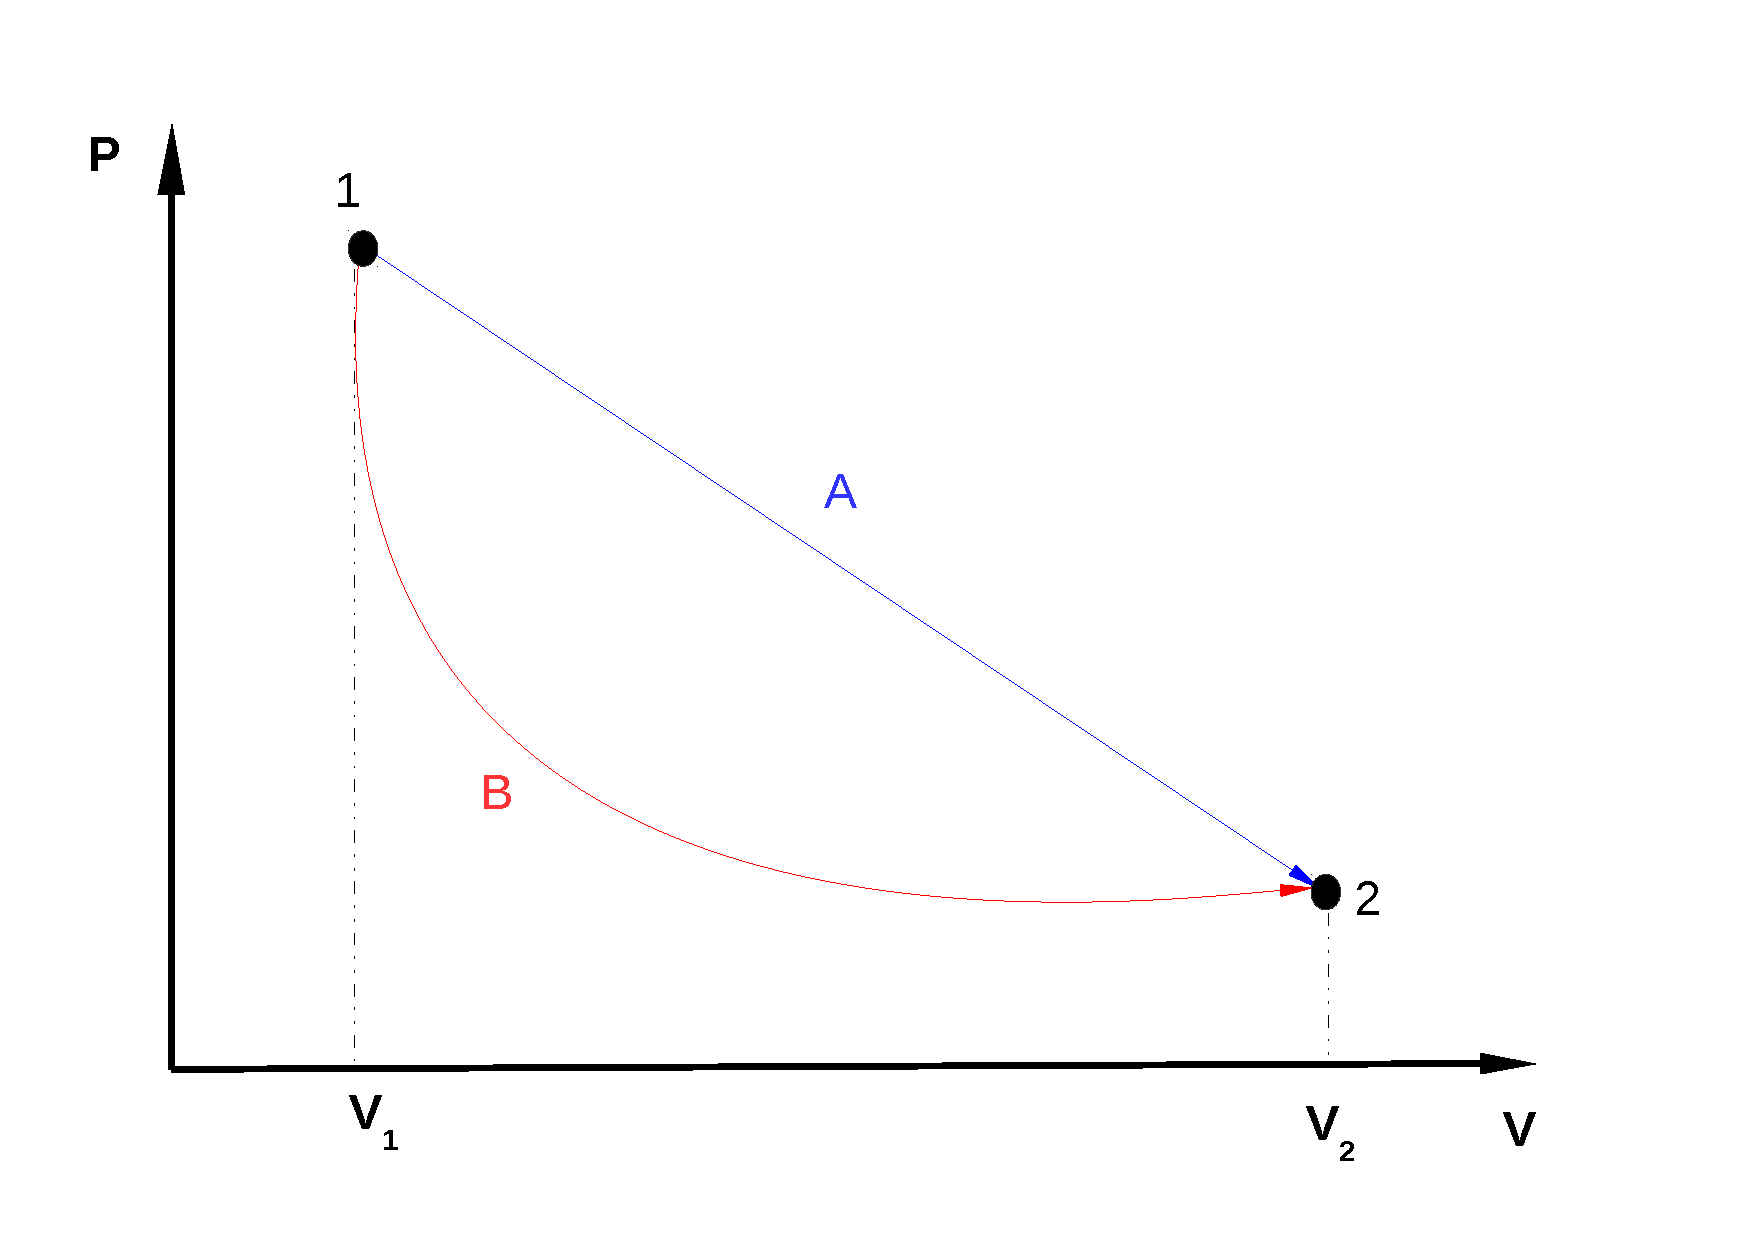
\includegraphics[width=0.7\columnwidth,clip]{./Figs/Chp3_PistonCylinder_PV}}}
        \caption{Gas expansion under different conditions represented by 2 paths.}\label{Chapter:FirstLaw:Fig:Work_PV}
   \end{figure}

   
%%%
%%% SECTION
%%%
   \section{Reversible Adiabatic Processes}\label{Chapter:FirstLaw:Section:ReversibleAdiabaticProcesses}\index{Process!Adiabatic}
     \begin{subequations}

       A process is named {\it adiabatic} when no heat is transferred to or from the system (\ie $\delta Q$ = 0),
         \begin{equation}
           dU = \cancelto{0}{\delta Q} + \delta W \;\;\Longrightarrow\;\; \Delta U = U_{2}-U_{1}= W.
         \end{equation}
       This equation is valid for both reversible and irreversible processes\index{Process!Reversible}\index{Process!Irreversible}, and can only be ensured if a perfect thermal insulation is achieved.  For mechanically reversible adiabatic (\ie isentropic) compression / expansion of ideal gases,
      \begin{eqnarray}
          dU &=& \delta Q + \delta W \;\;\Longrightarrow \;\; \delta Q = C_{v}dT + PdV = 0 \nonumber \\
          dT &=& -\frc{P}{C_{v}}dV  \;\; \left(\text{Constraint: } C_{v}\ne 0\right) \nonumber \\
             &=& -\frc{RT}{V C_{v}}dV \;\; \Rightarrow \;\; \frc{dT}{T} = - \frc{R}{C_{v}}\frc{dV}{V}. \label{Chapter:FirstLaw:Eqn:AdiabaticProcesses1}
      \end{eqnarray}
      Integrating Eqn.~\ref{Chapter:FirstLaw:Eqn:AdiabaticProcesses1} and assuming $C_{v}$ is constant,
           \begin{eqnarray}
              &&\int\limits_{T_{1}}^{T_{2}} \frc{dT}{T} = \frc{R}{C_{v}}\int\limits_{V_{1}}^{V_{2}}\frc{dV}{V} \;\;\Longrightarrow\;\;  \left.\ln{T}\right|_{T_{1}}^{T_{2}} = \left.-\frc{R}{C_{v}}\ln{V}\right|_{V_{1}}^{V_{2}}\nonumber \\
              &&\ln{\frc{T_{2}}{T_{1}}} = -\frc{R}{C_{v}}\ln{\frc{V_{2}}{V_{1}}} = \ln{\left(\frc{V_{1}}{V_{2}}\right)^{\frac{R}{C_{v}}}}\;\;\Longrightarrow\;\; \frc{T_{2}}{T_{1}} = \left(\frc{V_{1}}{V_{2}}\right)^{\frac{R}{C_{v}}} \nonumber
           \end{eqnarray}
           Now, using the ratio of specific heats defined in Eqn.~\ref{Chapter:FirstLaw:Eqn:HeatCapacitiesRelation_IdealGas2}, 
           \begin{displaymath}
              \gamma = 1 + \frc{R}{C_{v}},
           \end{displaymath}
           in the previous relation,
           \begin{shaded}
             \begin{equation}
                TV^{\gamma-1} = \text{ constant}\label{Chapter:FirstLaw:Eqn:AdiabaticProcesses_TVGamma}
             \end{equation}
           \end{shaded}

           Now from Eqn.~\ref{Chapter:FirstLaw:Eqn:HeatCapacitiesRelation_IdealGas3},
           \begin{displaymath}
               \delta Q = C_{p}dT - \frc{RT}{P}dP = 0,
           \end{displaymath}
           and assuming $C_{p}$ is constant and different from zero,
           \begin{eqnarray}
             && \int\limits_{T_{1}}^{T_{2}}\frc{dT}{T} = \frc{R}{C_{p}}\int\limits_{P_{1}}^{P_{2}}\frc{dP}{P} \;\;\Longrightarrow\;\; \left.\ln{T}\right|_{T_{1}}^{T_{2}} = \left.\frc{R}{C_{p}} \ln{P}\right|_{P_{1}}^{P_{2}} \nonumber \\
             && \ln{\frc{T_{2}}{T_{1}}} = \ln{\left(\frc{P_{2}}{P_{1}}\right)^{\frac{R}{C_{p}}}} \;\;\Longrightarrow\;\;  \frc{T_{2}}{T_{1}} = \left(\frc{P_{2}}{P_{1}}\right)^{\frac{R}{C_{p}}}.\nonumber
           \end{eqnarray}
           Again, using  Eqn.~\ref{Chapter:FirstLaw:Eqn:HeatCapacitiesRelation_IdealGas2},
           \begin{shaded}
             \begin{equation}
                TP^{\frac{1-\gamma}{\gamma}} = \text{ constant}\label{Chapter:FirstLaw:Eqn:AdiabaticProcesses_TPGamma}
             \end{equation}
           \end{shaded}
           
           Finally, integrating the right-hand side from Eqn.~\ref{Chapter:FirstLaw:Eqn:HeatCapacitiesRelation_IdealGas3},
           \begin{eqnarray}
               && \delta Q = \frc{C_{v}}{R}VdP + \frc{C_{p}}{R}PdV = 0 \;\; \Longrightarrow \;\; \frc{C_{v}}{\cancel{R}}VdP = -\frc{C_{p}}{\cancel{R}}PdV \;\;\Longrightarrow\;\; C_{v}\int\limits_{P_{1}}^{P_{2}} \frc{dP}{P} = -C_{p}\int\limits_{V_{1}}^{V_{2}}\frc{dV}{V} \nonumber \\
              && \left.\ln{P}\right|_{P_{1}}^{P_{2}} = -\left.\frc{C_{p}}{C_{v}}\ln{V}\right|_{V_{1}}^{V_{2}} \;\; \Longrightarrow \;\;\frc{P_{2}}{P_{1}} = \left(\frc{V_{1}}{V_{2}}\right)^{\frac{C_{p}}{C_{v}}}\nonumber 
           \end{eqnarray}
           Again, using  Eqn.~\ref{Chapter:FirstLaw:Eqn:HeatCapacitiesRelation_IdealGas2},
           \begin{shaded}
             \begin{equation}
                PV^{\gamma} = \text{ constant}\label{Chapter:FirstLaw:Eqn:AdiabaticProcesses_PVGamma}
             \end{equation}
           \end{shaded}
     \end{subequations}



   % Example
   \begin{MyExample}{\begin{center}{\bf Example}\end{center}}
     \begin{example}\label{Chapter:FirstLaw:Example8}\citep{Rajput_Book}
       Air initially occupying 1 m$^{3}$ at 1.5 bar and 20$^{\circ}$C undergoes an internally reversible compression for which $P V^{\gamma}=$ constant to a final state where the pressure is 6 bar and the temperature is 120$^{\circ}$C. Determine:
        \begin{enumerate}[(a)]
           \item Value of $\gamma$;
           \item Work and the heat transfer (in kJ).
       \end{enumerate}
       Assume that heat capacity at constant volume and molar mass of air are 0.718 kJ.$\left(\text{kg.K}\right)^{-1}$ and 29 g.mol$^{-1}$.
     \end{example}

% SOLUTION
       \noindent{\bf Solution:} 
        \begin{center}
           \begin{tabular}{c c c c}
               {\bf State}  &   $P$ (atm)  &   $T\;\left(^{\circ}\text{C}\right)$ & $V\;\left(\text{m}^{3}\right)$ \\
                    1       &     1.5      &            20                      & 1  \\
                    2       &     6.0      &            120                     &     \\              
           \end{tabular}
        \end{center}
        \begin{enumerate}[(a)]
           \item In order to calculate the isentropic index $\gamma$, we can use any of the relations learned in the lecture,
               \begin{displaymath} 
                   P V^{\gamma} = C, \hspace{1cm} T V^{\gamma-1} = C \hspace{1cm} \text{ and/or } \hspace{1cm} T P^{\frac{1-\gamma}{\gamma}} = C.
               \end{displaymath}
               Although $P$ and $V$ is the relation initially given in the problem, we do not know the final volume of air, $V_{2}$. However, initial and final pressure and temperature are known and we can make use of this relationship to obtain $\gamma$,
               \begin{eqnarray} 
                   T P^{\frac{1-\gamma}{\gamma}} = C \Rightarrow T_{1}P_{1}^{\frac{1-\gamma}{\gamma}} = T_{2}P_{2}^{\frac{1-\gamma}{\gamma}} \nonumber \\
                   \left(\frc{P_{1}}{P_{2}}\right)^{\frac{1-\gamma}{\gamma}} = \frc{T_{2}}{T_{1}} \Rightarrow \frc{1-\gamma}{\gamma} = \frc{\ln{\frac{T_{2}}{T_{1}}}}{\ln{\frac{P_{1}}{P_{2}}}} \Longrightarrow \gamma = 1.2686  \nonumber
               \end{eqnarray}
                 
           \item Compression work can be obtained by integrating $\d W = -P dV$ from state 1 to state 2 with $P=\frac{C}{V^{\gamma}}$,
               \begin{eqnarray}
                 W_{1-2} &=& -\int\limits_{V_{1}}^{V_{2}} P dV = -\int\limits_{V_{1}}^{V_{2}}\frc{C}{V^{\gamma}} dV = -\left.\frc{C}{1-\gamma}V^{1-\gamma}\right|_{V_{1}}^{V_{2}} \nonumber \\
                         &=& -\frc{C}{1-\gamma}\left(V_{2}^{1-\gamma}-V_{1}^{1-\gamma}\right),\;\;\text{ however, as } C=P_{1}V_{1}^{\gamma}=P_{2}V_{2}^{\gamma} \nonumber \\
                         &=& -\frc{P_{2}V_{2}^{\gamma}V_{2}^{1-\gamma} - P_{1}V_{1}^{\gamma}V_{1}^{1-\gamma}}{1-\gamma} = \frc{P_{1}V_{1}-P_{2}V_{2}}{1-\gamma} \nonumber
               \end{eqnarray}
               The relation above, although important, can not be used as we do not know $V_{2}$, however we can change variables through the ideal gas relation
               \begin{eqnarray}
                 P V = n R T &\Rightarrow& n = \frc{P V}{R T } = \frc{1.5\text{ atm} \times 1\text{ m}^{3}}{ 8.3143 \frc{\text{J}}{\text{mol.K}} 293.15\text{ K}} \frc{1.01325\times 10^{5} \text{ Pa}}{1 \text{ atm}} \frc{ 1 \text{ N.m}^{-2}}{1\text{ Pa}}\frc{1 \text{ J}}{1\text{ N.m}} \nonumber \\
                 &&  n = 62.3580\text{ moles} \nonumber \\
                   % m &=& \frc{P_{1} V_{1} MW}{R T_{1}} = \frc{1.5\text{ atm} \times 1\text{ m}^{3} \times 29 \frac{\text{g}}{\text{mol}} } { 8.3143 \frc{\text{J}}{\text{mol.K}} 293.15\text{ K}} \frc{1 \text{ J}}{1\text{ N.m}} \frc{1.01325\times 10^{5} \text{ Pa}}{1 \text{ atm}} \frc{ 1 \text{ N.m}^{-2}}{1\text{ Pa}} = 1808.38 \text{ g}\nonumber\\
                    W &=& \frc{P_{1}V_{1}-P_{2}V_{2}}{1-\gamma} = nR\frc{T_{1}- T_{2}}{1-\gamma} \nonumber \\
                      &=& 62.3580\text{ mol} \times 8.3143 \frc{\text{J}}{\text{mol.K}} \times \frc{\left(293.15-393.15\right)\text{ K}}{1-1.2686} \nonumber \\
                      &=& 193024.2440 \text{ J} \Longrightarrow W = -193.02 \text{ kJ} \nonumber
               \end{eqnarray}
              Heat ($Q$) can be obtained from
               \begin{eqnarray}
          \Delta u &=& m C_{v}\Delta T = n MW C_{v}\Delta T = Q + W  \nonumber \\
             Q &=& n MW C_{v}\left(T_{2}-T_{1}\right) - W \nonumber \\
               &=& 62.3580\text{ mol}\times 29 \frc{\text{g}}{\text{mol}} \red{\frc{1\text{ kg}}{1000\text{ g}}}\times 0.718\frc{\text{kJ}}{\text{kg.K}}\times (393.15-293.15)\text{ K} - 193.30 \text{ kJ} \nonumber \\
                                                          &=& -63.46\text{ kJ}. \nonumber                   
               \end{eqnarray}
        \end{enumerate}
   \end{MyExample}
   

   
\clearpage   
\begin{FinalSummaryBlock}{Summary}
    \begin{itemize}
       \item Work is the transfer of energy by motion against an opposing force;
       \item Heat is the transfer of energy as a result of temperature differences between the system and the surroundings;
       \item Internal energy is the energy stored in the components of the system. The internal energy of an ideal gas is a function of temperature only;
       \item The First Law of thermodynamics states that heat and work are mutually convertible, however as energy can not be either created or destroyed, the internal energy associated with an energy conversion remains constant, $dU = \delta q + \delta w$;
       \item The energy of an isolated system is always constant;
       \item A reversible change is a change that can be reversed by an infinitesimal modification of a variable. Maximum work is achieved in a reversible change;
       \item The enthalpy is defined as $H = U + PV$. The enthalpy change is the energy transferred as heat at constant pressure, $\Delta H = Q$;
       \item Heat capacity at constant volume is defined as $C_{v}=\left(\partial U / \partial T\right)_{V}$. The heat capacity at constant pressure is defined as $C_{p}=\left(\partial H / \partial T\right)_{P}$;
       \item In case of:
         \begin{itemize}
            \item Reversible isochoric process (\ie $V=$ constant):
              \begin{displaymath}
                \Delta U = C_{v}\left(T_{2}-T_{1}\right), \;\; W = 0\;\; Q = C_{v}\left(T_{2}-T_{1}\right);
              \end{displaymath}
            \item Reversible isobaric process (\ie $P=$ constant):
              \begin{displaymath}
                \Delta U = C_{v}\left(T_{2}-T_{1}\right), \;\; W = P\left(V_{2}-V_{1}\right)\;\; Q = C_{p}\left(T_{2}-T_{1}\right);
              \end{displaymath}
            \item Reversible adiabatic process (\ie $PV^{\gamma}=$ constant):
              \begin{displaymath}
                 \frc{T_{2}}{T_{1}} = \left(\frc{V_{1}}{V_{2}}\right)^{\gamma-1} = \left(\frc{P_{2}}{P_{1}}\right)^{\frc{\gamma-1}{\gamma}};
              \end{displaymath}
            \item Polytropic reversible process (\ie $PV^{n}=$ constant):
              \begin{displaymath}
                 \frc{T_{2}}{T_{1}} = \left(\frc{V_{1}}{V_{2}}\right)^{n-1} = \left(\frc{P_{2}}{P_{1}}\right)^{\frc{n-1}{n}}.
              \end{displaymath}
         \end{itemize}
    \end{itemize}
\end{FinalSummaryBlock}
 % Introduction to First Law of Thermodynamics
     \setcounter{examplecounter}{0}
  
%%%
%%% CHAPTER
%%%
\chapter{Second Law of Thermodynamics}\label{Chapter:FirstLaw}

   \begin{LearningObjectivesBlock}{Learning Objectives}
      Upon completion of this chapter, you will be able to
        \begin{enumerate}
           \item Demonstrate understanding of key concepts of energy and the first law of thermodynamics;
           \item Apply the first law of thermodynamics to assess of heat transfer and power cycles;
           \item Conduct energy analysis of thermodynamic systems;
           \item Employ energy and mass balances into thermodynamic systems to assess efficiency, and correctly observe sign conventions for work and heat transfer.
        \end{enumerate}
\medskip
     Recommended reading: Chapters 5 of \citet{SmithVanNess_Book,Moran_Book,Borgnakke_Book} or 3 of \citet{Atkins_Book}.
   \end{LearningObjectivesBlock}


  
%%%
%%% SECTION
%%%
   \section{Introduction}\label{Chapter:SecondLaw:Section:Intro}
   The first law (Chapters~\ref{Chapter:Introduction} and \ref{Chapter:FirstLaw}) demonstrated that energy can flow either from or to a system in the form of heat or work, however it does not indicate the direction of process (\ie energy flow). The second law of thermodynamics concerns about feasibility, direction and spontaneity of processes and entropy..
   
The second law of thermodynamics is a general principle which makes constraints upon spontaneity of the process, direction of heat transfer and general efficiency of heat engines, \eg a hot body cools to the temperature of the surroundings or a chemical reaction that may run in one direction instead of the reverse (\eg combustion of ethane producing carbon dioxide and water). The reverse of such processes may occur but they will not be spontaneous.  
  
%%%
%%% SECTION
%%%
   \section{Statement of the Second Law}\label{Chapter:SecondLaw:Section:SecondLawStatement}\index{Laws of Thermodynamics ! Second law}
The second law of thermodynamics was stated separately by \citet{Clausius_Book}, Kelvin \citep{Thomson_1851} and \citet{Planck_Book} in slightly different ways. Each statement is based on irreversible processes.
\begin{shaded}
  \begin{center}
    {\bf Clausius Statement}
  \end{center}
  'It is impossible for a self-acting machine working in a cyclic process unaided by any external agency, to convey heat from a body at a lower temperature to a body at a higher temperature.'
\end{shaded}
This statement clearly indicates that heat cannot spontaneously flow from a colder to a hotter body. This can only be realised if other effects play some role, \eg in a refrigeration process in which external work is used to extract heat from low temperature body and reject it into a high temperature body (Fig.~\ref{Chapter:SecondLaw:Fig:SecondLawStatement})

   %%% FIGURE
   \begin{figure}[h]
     \begin{center}
        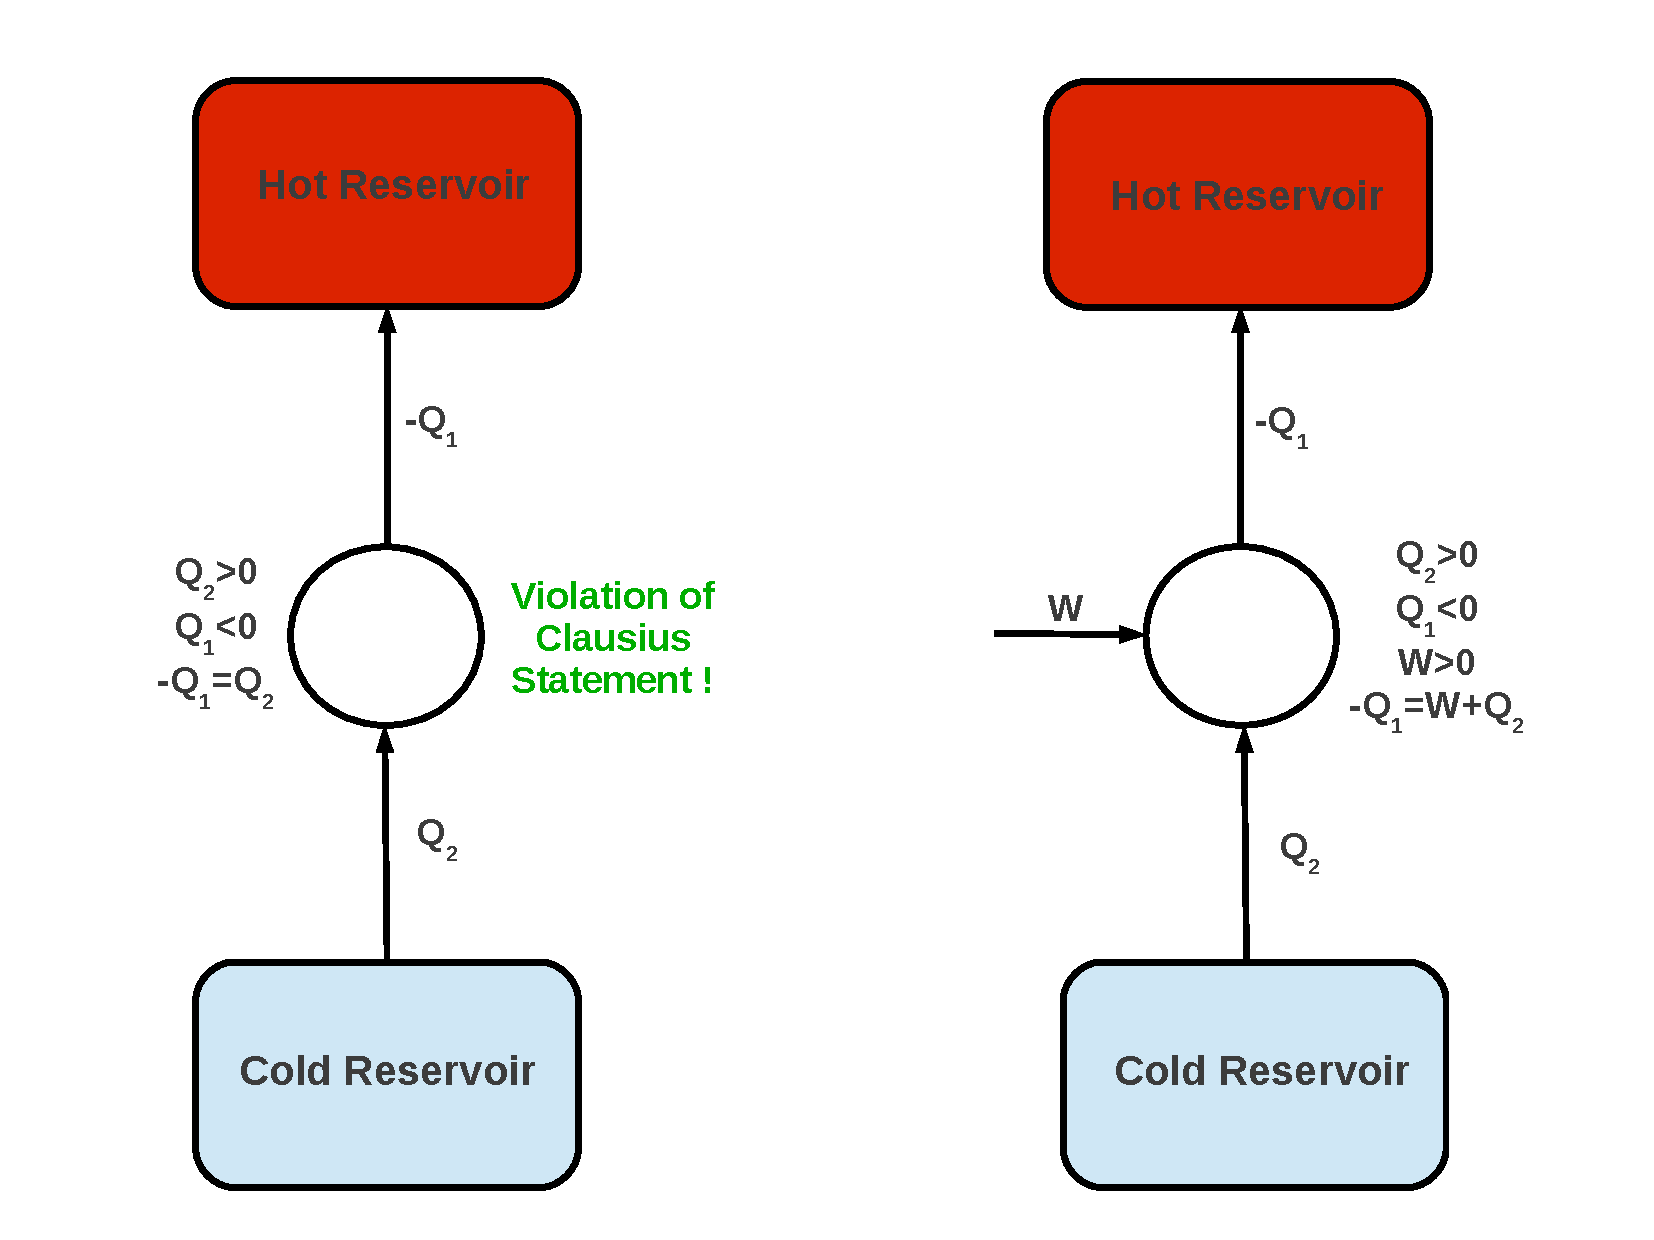
\includegraphics[width=.8\columnwidth,clip]{./Figs/2ndLaw_Schem}
     \caption{All spontaneous processes are irreversible -- heat flows from hot to cold spontaneously and irreversibly. }\label{Chapter:SecondLaw:Fig:SecondLawStatement}
     \end{center}
   \end{figure} 

\begin{shaded}
  \begin{center}
    {\bf Kelvin-Planck Statement}
  \end{center}
  'It is impossible to construct an engine, which while operating in a cycle produces no other effect except to extract heat from a single reservoir and do equivalent amount of work.'
\end{shaded}
This statement indicates that in order to achieve net work from a heat engine (\ie a device operating in cycle), there should be heat interaction between two bodies (\ie thermal reservoirs) at different temperatures (\ie thermal source or sink). 


%%%
%%% SECTION
%%%
   \section{Mathematical Statement of the Second Law}\label{Chapter:SecondLaw:Section:SecondLawStatement_Maths}\index{Laws of Thermodynamics ! Second law}
     \begin{subequations}
        In Fig.~\ref{Chapter:SecondLaw:Fig:SecondLawStatement2}, an infinitesimal amount of heat, $\delta Q^{\prime}$, is transferred from the thermal reservoir (with temperature $T_{res}$) to a reversible cyclic engine (1). The engine produces a small amount of work, $\delta W^{\prime}$, and releases an infinitesimal amount of heat, $\delta Q$ to another reservoir (at variable temperature $T$) that also releases energy in form of work $\left(\delta W\right)$ to the surroundings.


   %%% FIGURE
   \begin{figure}[h]
     \begin{center}
        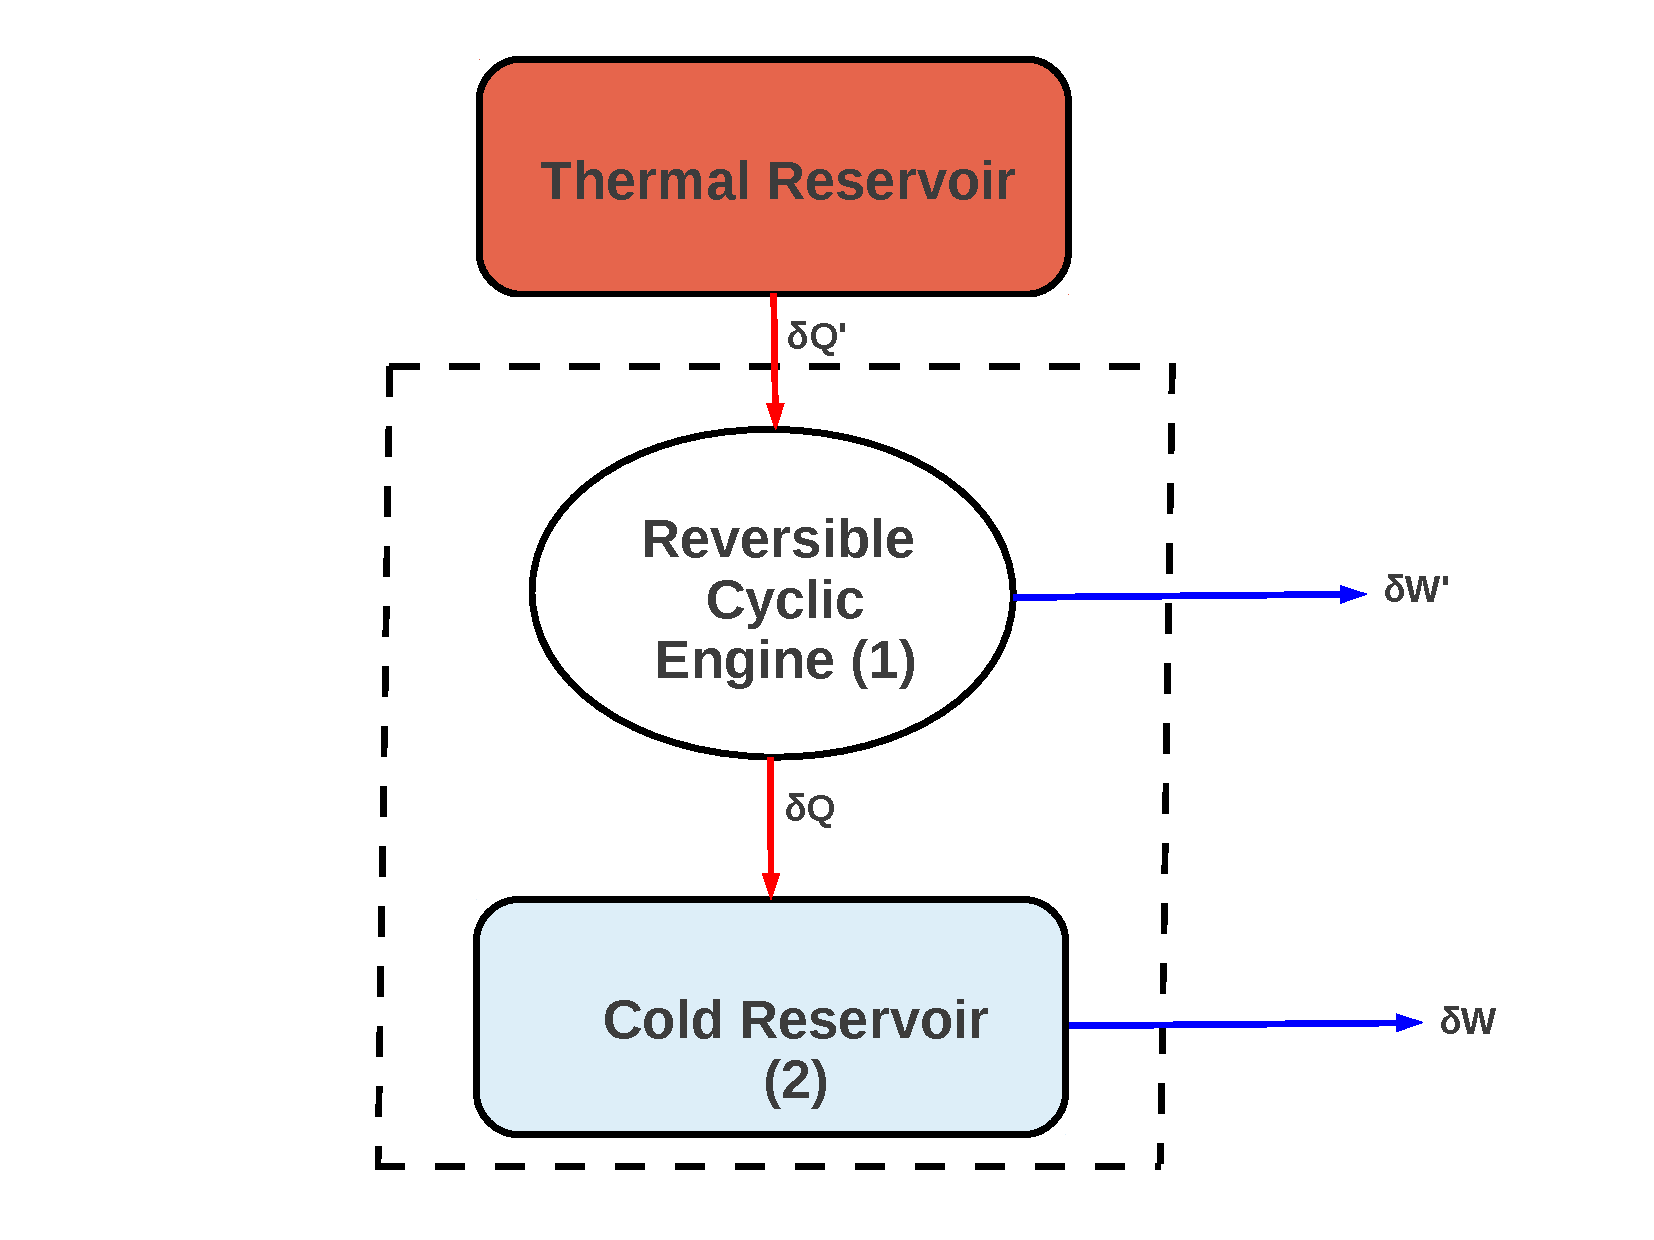
\includegraphics[width=.8\columnwidth,clip]{./Figs/2ndLaw_Schem2}
     \caption{Thermal device for mathematical derivation of the Second law. }\label{Chapter:SecondLaw:Fig:SecondLawStatement2}
     \end{center}
   \end{figure} 

     \end{subequations}
 % Introduction to Second Law of Thermodynamics

\part{Thermodynamic Properties of Fluids}  
     \setcounter{examplecounter}{0}
  \chapter{Volumetric Properties of Pure Substances}\label{Chapter:VolumetricPropertiesPureSubstances}

   \begin{LearningObjectivesBlock}{Learning Objectives}
      Upon completion of this chapter, you will be able to
        \begin{enumerate}
           \item Define pure substances and thermodynamic phases;
           \item State the Gibbs phase rule and its use to define the number of degrees of freedom of a system;
           \item Identify phases and phase transitions in a diagram;
           \item Formulate the solution for thermodynamic problems involving the calculation of volume of pure substances;
           \item Select appropriate equation of state for a given problem/application;
        \end{enumerate}
\medskip
     Recommended reading: Chapters 3 of \citet{SmithVanNess_Book}, 6 of \citet{Sandler_Book}, 2 of \citet{Borgnakke_Book}, 11 of \citet{Moran_Book} or 4 of \citet{Atkins_Book}.
   \end{LearningObjectivesBlock}


%%%%%%%%%%%%%%%%%%%%%%%%%%%%%%%%%%%%%%%%%%%%%%%%%%%%%%%%%%%%%%%%%
\begin{comment}
   \begin{LearningObjectivesBlock}{Learning Objectives}
      Upon completion of this chapter, you will be able to
        \begin{enumerate}
           \item {\bf Knowledge:} Define, Name, Select, State 
           \item {\bf Comprehension:} Describe, Identify, Discuss
           \item {\bf Application:} Apply, Demonstrate, Employ, Sketch
           \item {\bf Analysis:} Analyse, Compare, Calculate, Solve
           \item {\bf Synthesis:} Determine, Formulate
           \item {\bf Evaluation:} Assess, Check, Estimate, Compare, Measure, Monitor
        \end{enumerate}
\end{comment}
%%%%%%%%%%%%%%%%%%%%%%%%%%%%%%%%%%%%%%%%%%%%%%%%%%%%%%%%%%%%%%%%%
  

%%%% ETOC
\localtableofcontents

%%%
%%% SECTION
%%%
   \section{Introduction}\label{Chapter:VolumetricPropertiesPureSubstances:Section:Intro}
   Definitions and assumptions for ideal gas behaviour were introduced in Section~\ref{Chapter:Intro_Property_of_Gases:Section:IdealGases} along with the corresponding equation of state (Eqn.~\ref{Chapter:Intro_Property_of_Gases:Eqn:IdealEOS}). A fluid behaves as an ideal gas at low to moderate pressures (often below atmospheric pressure) and at high temperatures. Under realistic environmental and industrial conditions, fluids may not behave as ideal gases and therefore other equations of state (not just for gases) were designed to describe the {\it PVT} behaviour of fluids.

Phase transition of pure substances is one of the main topics in industrial chemical engineering as it is of paramount importance to calculate fluid properties for the design of equipment and processes. Therefore, the main aim of this chapter is to introduce the concept of phase diagram of pure substances and its mathematical representation as equations of state. 

  
%%%
%%% SECTION
%%%
   \section{Phase Diagrams of Pure Substances}\label{Chapter:VolumetricPropertiesPureSubstances:Section:PhaseDiagrams}\index{Phase diagram}\index{Triple point}\index{Supercritical state}

Pure substances/fluids can be defined as materials of homogeneous and constant composition. For example, systems containing water-ice, water-steam or water-ice-steam are considered pure fluids (or substances) at different phases, whereas (a) air-water, (b) air-steam and (c) gaseous mixture containing N$_{2}$, H$_{2}$, O$_{2}$ and NO$_{2}$ are considered as either homogeneous (b-c) or heterogeneous (a) mixtures.

A pure substance can exist and coexist in different phases\footnote{Phase of a substance can be defined as the form of matter that is uniform in chemical composition and physical state.}  (\ie solid, liquid and vapour -- S, L and V). Phase behaviour of substances is often represented by {\it PVT}~\footnote{{\it PVT} stands for pressure, specific (or molar) volume and temperature.} phase diagrams that describe phase transitions (\ie spontaneous conversion -- or mass/heat transfer of one phase to another) and coordinates. A 3D {\it PVT} diagram of an arbitrary substance is shown in Figure~\ref{Chapter:VolumetricPropertiesPureSubstances:Fig:PVT_Surfaces}a, where solid, liquid and vapour phases are represented by continuous volumes and, the regions between these volumes are representations of phase equilibrium, \ie regions where phases coexist in thermodynamic equilibrium.

   %%% FIGURE
           \begin{figure}[h]
              \begin{center}
                 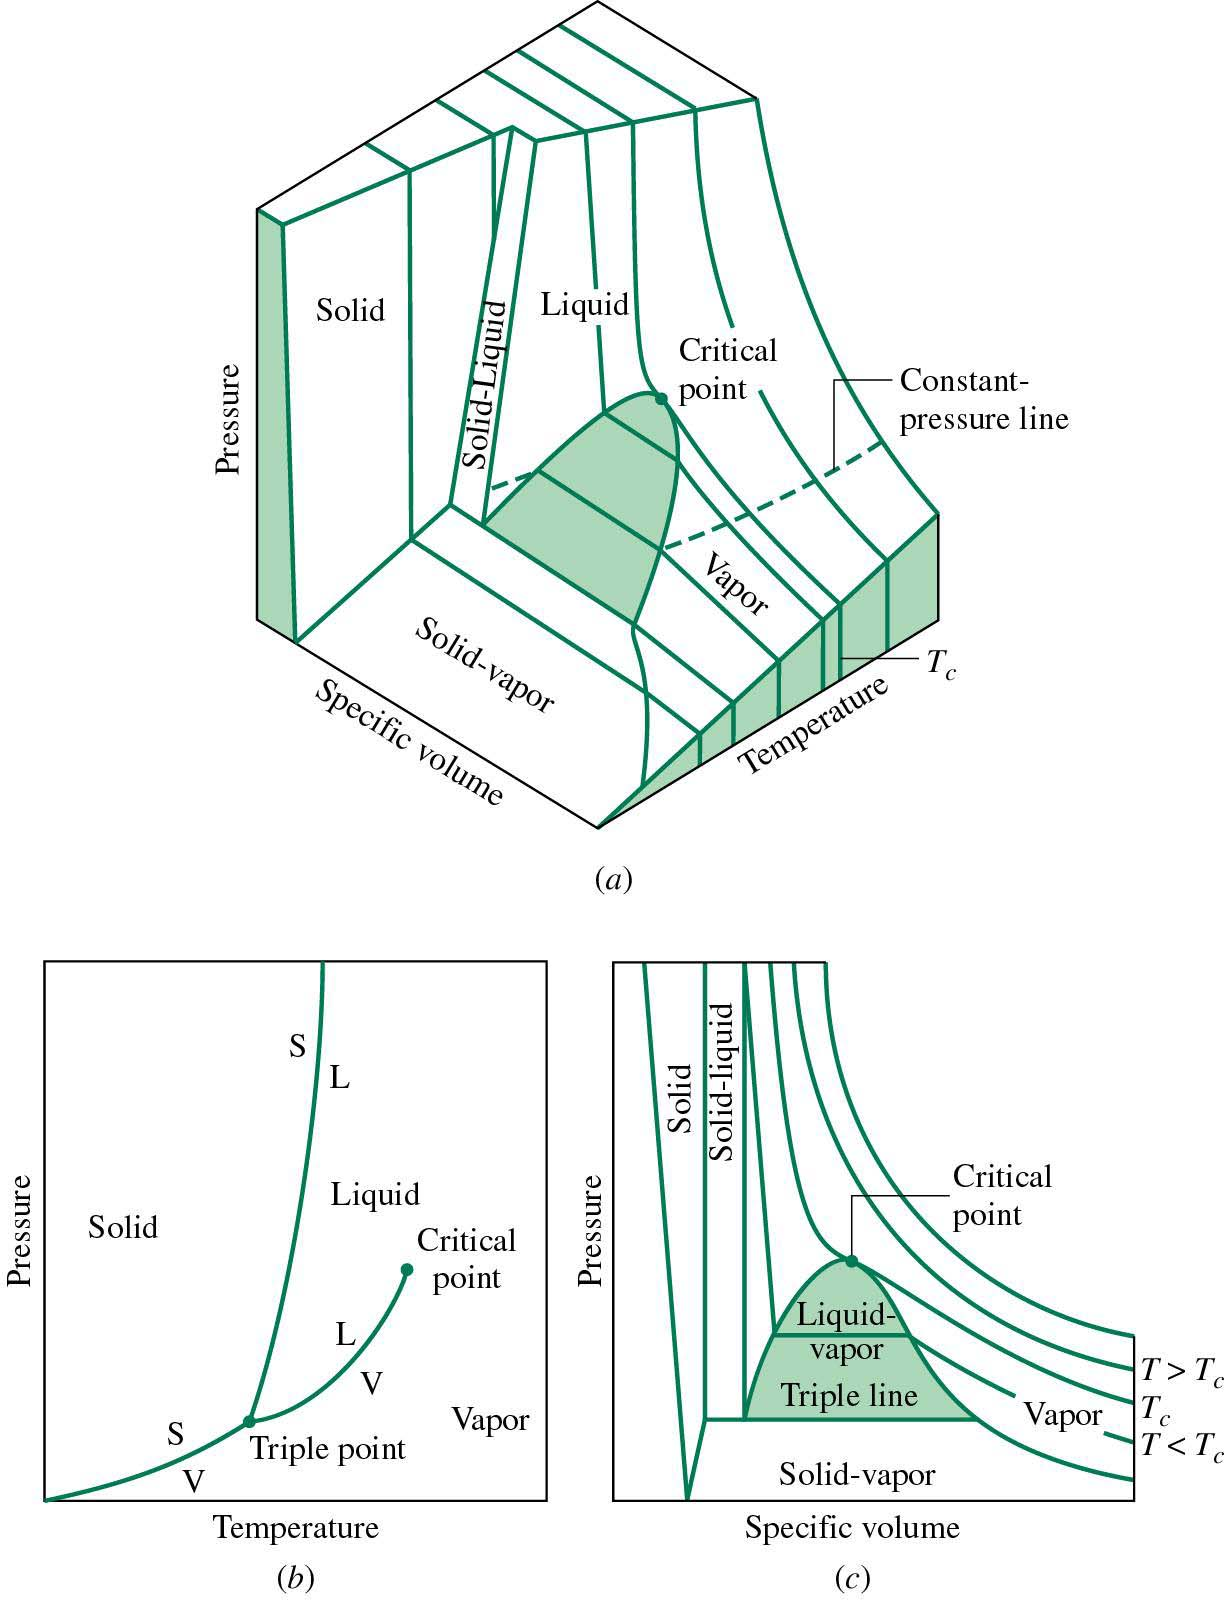
\includegraphics[width=10.cm,clip]{./Figs/PVT_Surface.jpg}
                 \caption{$PVT$ volume (top) and projections onto (b) $PT$ and (c) $PV$ diagrams for a pure substance \citep[Extracted from][]{Borgnakke_Book}.}\label{Chapter:VolumetricPropertiesPureSubstances:Fig:PVT_Surfaces}
              \end{center}
           \end{figure}    

Such 3D representation helps to qualitatively determine fluid phases (S, L and V) at prescribed coordinates (temperature, specific/molar volume and pressure). However, it is not convenient dealing with 3D plots and, most of the time, we may want to extract quantitative values of fluids (Chapter~\ref{Chapter:ThermodynamicPropertiesPureFluids}). A better approach is to project 3D plots into surfaces, \ie through $PT$, $PV$ and $VT$ phase diagrams as shown in Figs.~\ref{Chapter:VolumetricPropertiesPureSubstances:Fig:PVT_Surfaces}b and \ref{Chapter:VolumetricPropertiesPureSubstances:Fig:PVT_Surfaces}c.

$PV$ diagrams (\eg Fig.~\ref{Chapter:VolumetricPropertiesPureSubstances:Fig:PV-PT_Diagrams}a) are representations of the PVT diagram, Fig.~\ref{Chapter:VolumetricPropertiesPureSubstances:Fig:PVT_Surfaces}a, where surfaces (\ie areas) represent both single phases and phases in equilibrium, and lines represent transition between phases. Here, there are three properties that we need to define:
           \begin{enumerate}[a)]
              \item Critical point (or state): coordinates in which two phases of a fluid become indistinguishable (`C' in Fig.~\ref{Chapter:VolumetricPropertiesPureSubstances:Fig:PV-PT_Diagrams}a) . Beyond this coordinate, a fluid is neither completely liquid nor completely gaseous, \ie exhibits properties of both liquid and gas phases and is referred to as a {\it supercritical fluid}. All fluids have distinct critical coordinates, known as {\it critical pressure} $\left(\text{P}_{c}\right)$, {\it critical temperature} $\left(\text{T}_{c}\right)$ and {\it critical volume} $\left(\text{V}_{c}\right)$. Interesting videos about critical state can be seen in 
                  \begin{center}
                     \href{https://www.youtube.com/watch?v=bJjcTpRzXpM}{https://www.youtube.com/watch?v=bJjcTpRzXpM} and \\
                     \href{https://www.youtube.com/watch?v=RmaJVxafesU}{https://www.youtube.com/watch?v=RmaJVxafesU}.
                  \end{center}
              \item Saturation lines (blue lines in Fig.~\ref{Chapter:VolumetricPropertiesPureSubstances:Fig:PV-PT_Diagrams}a) are coordinates in which phase transition starts to occur.
              \item Isotherms: Lines of constant temperature (dotted line in Fig.~\ref{Chapter:VolumetricPropertiesPureSubstances:Fig:PV-PT_Diagrams}a) .
           \end{enumerate}

   %%% FIGURE
           \begin{figure}[h]
              \vbox{
                    \hbox{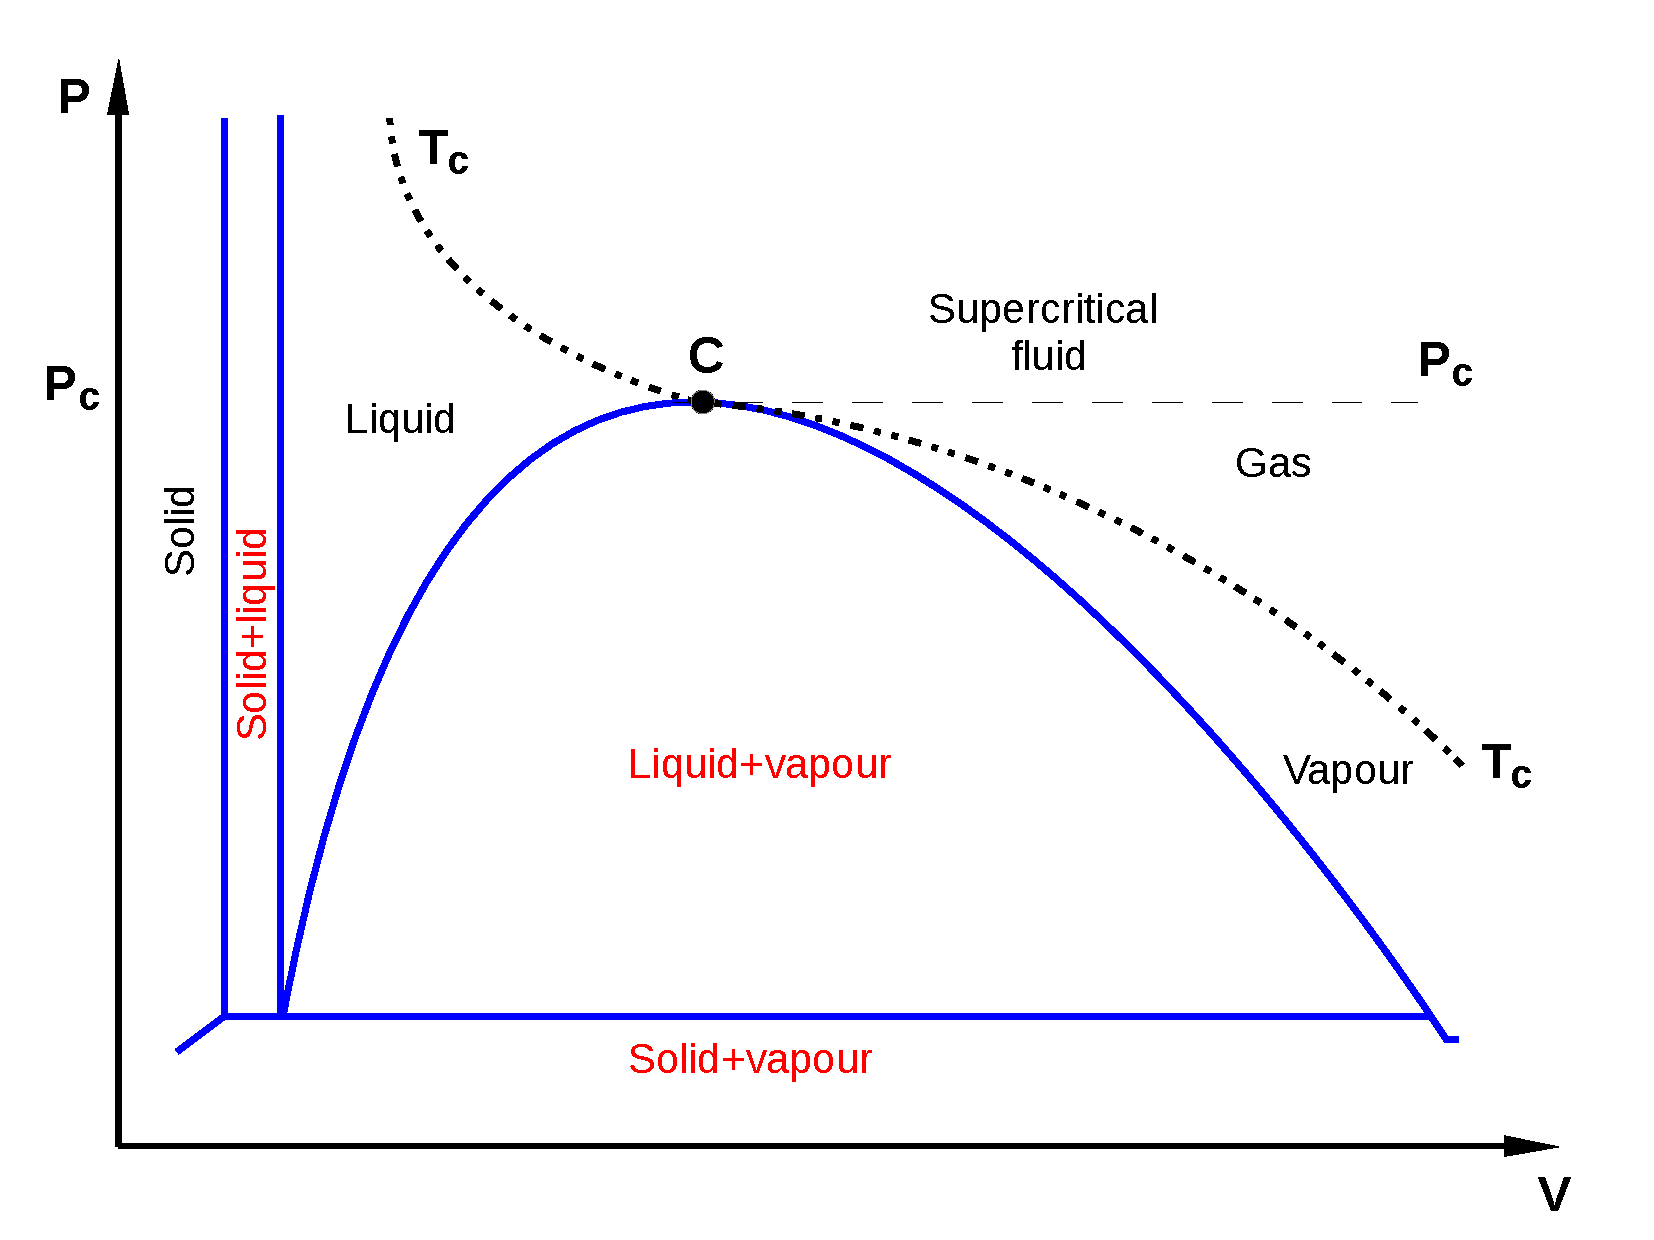
\includegraphics[width=.5\columnwidth,clip]{./Figs/PV_Diagram1}
                          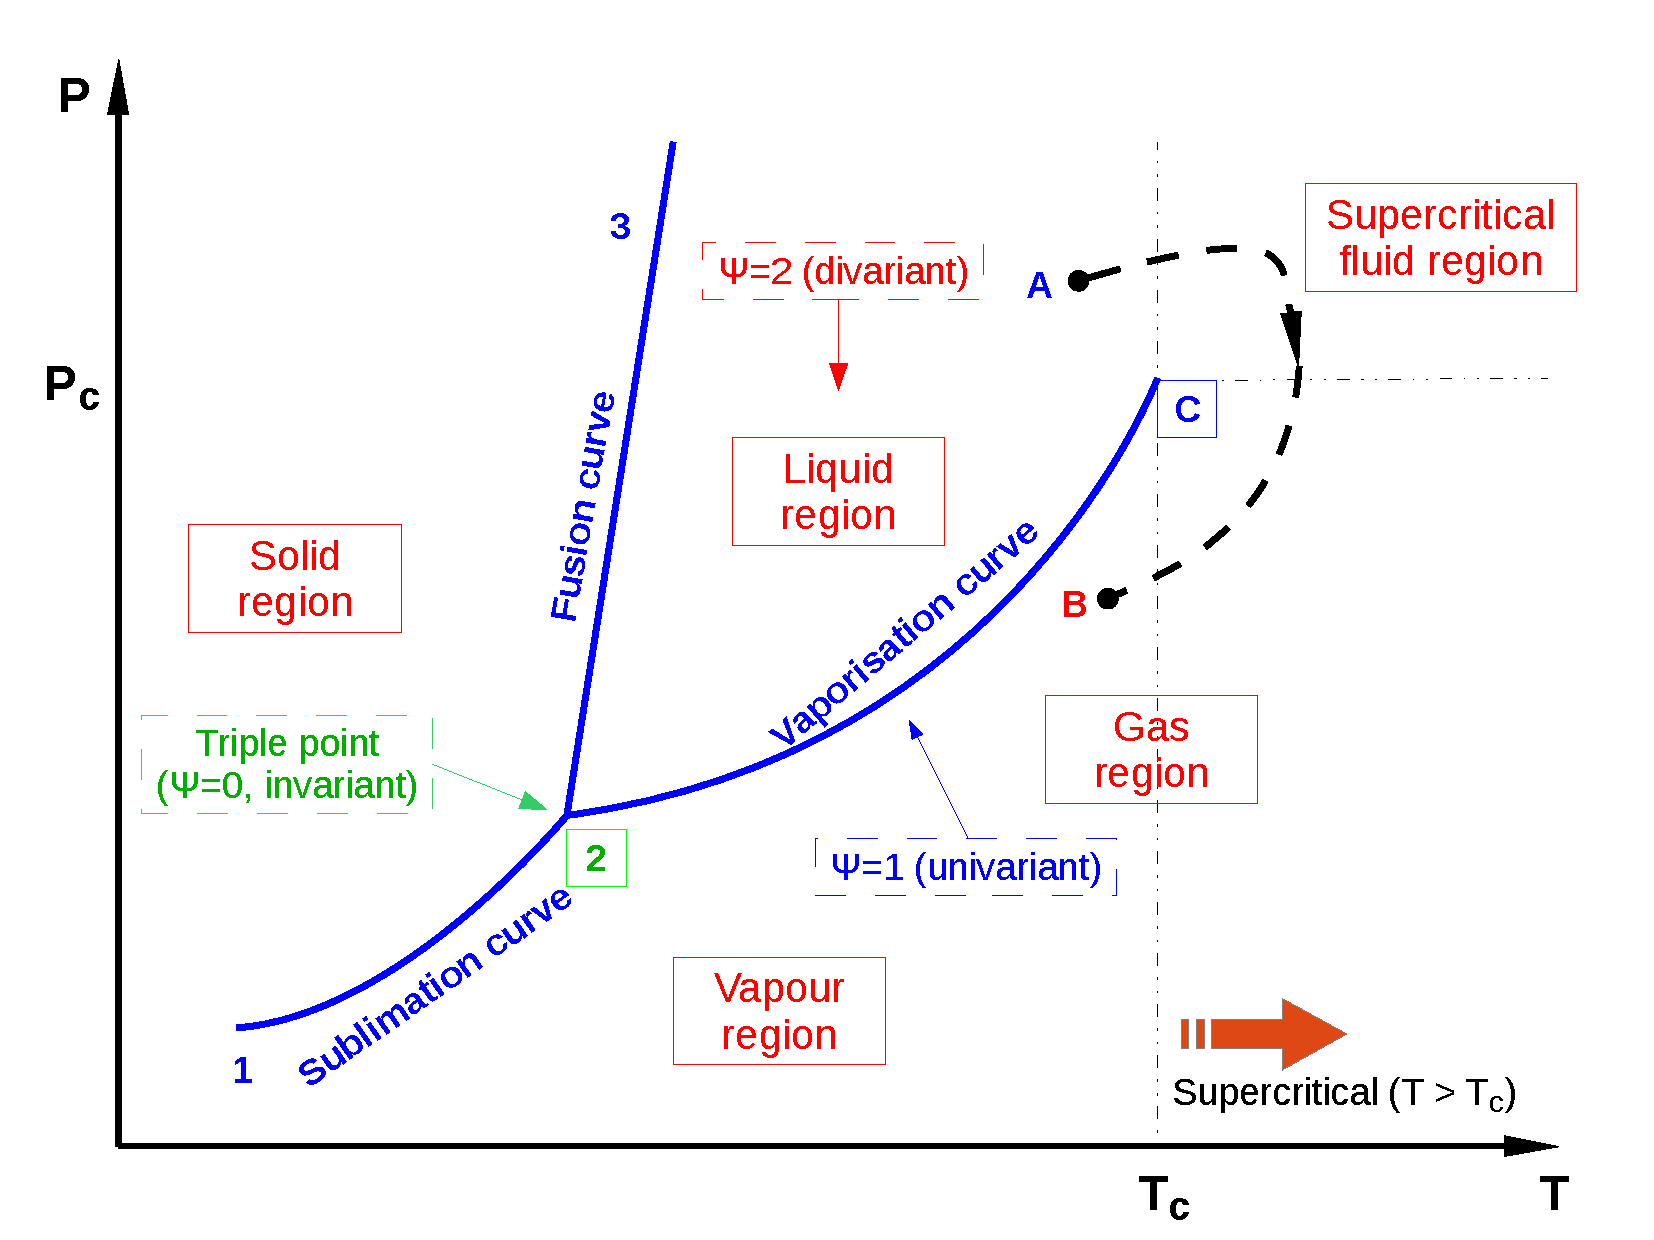
\includegraphics[width=.5\columnwidth,clip]{./Figs/PT_Diagram}}
                    \vspace{-.1cm}
                    \hbox{\hspace{4cm}(a)\hspace{8cm}(b)}}
              \caption{ (a) $PV$ and (b) $PT$ diagrams for a pure substance. Dotted line in (a) represents the isotherm at T=T$_{c}$.}\label{Chapter:VolumetricPropertiesPureSubstances:Fig:PV-PT_Diagrams}
           \end{figure}


           In vapour-liquid equilibrium (VLE) systems there are two main saturation lines: {\it saturated liquid line} (left-hand side of $C$ in Fig.~\ref{Chapter:VolumetricPropertiesPureSubstances:Fig:PV-PT_Diagrams}a)  and {\it saturated vapour line} (rhs of $C$) that represent the initial transition from a single phase system to a two/three-phases system. 
%

$PT$ diagrams (Fig.~\ref{Chapter:VolumetricPropertiesPureSubstances:Fig:PV-PT_Diagrams}b) are representations of Fig.~\ref{Chapter:VolumetricPropertiesPureSubstances:Fig:PVT_Surfaces}a, where phases are defined by surfaces (\ie areas) with continuous lines representing phases transitions (\ie in equilibrium). The {\it triple point} is the coordinate in which all three phases (S, L and V) coexist in equilibrium.

A fluid in the compressed liquid state is often called {\it sub-cooled fluid} (central region of Fig.~\ref{Chapter:VolumetricPropertiesPureSubstances:Fig:PV-PT_Diagrams}b), while a gas at a pressure lower than its saturation vapour pressure for a given temperature is said to be at {\it superheated state}.


%%% SECTION
%%%
\section{Gibbs Phase Rule}\label{Chapter:VolumetricPropertiesPureSubstances:Section:GibbsPhaseRule}\index{Phase rule}\index{Gibbs phase rule|see {Phase rule}}\index{Phase rule !Degrees of freedom}\index{Degrees of freedom|see {Phase rule}}
  In the $PT$ diagram (Fig.~\ref{Chapter:VolumetricPropertiesPureSubstances:Fig:PV-PT_Diagrams}b) of an arbirtrary pure substance, three regions may be clearly noted, liquid, vapor and solid. In order to fix any of such thermodynamic states, both temperature and pressure are needed, \ie a one-component, single phase system has two {\it degrees of freedom}. However, during phase transition (\eg vaporisation , fusion or sublimation lines), any change in pressure will lead to change in temperature in order to fix the thermodynamic state. Therefore, it is important to obtain precise information to set up a thermodynamic state of multi-component and multiphase systems.

  Let's consider a non-reactive system in equilibrium within $\mathcal{P}$ phases  (\ie $L$, $V$ and/or $S$) containing $\mathcal{C}$ independent chemical species.  The number of degrees of freedom $\left(\Psi\right)$ for the system (\ie the number of intensive variables that may vary independently) may be expressed as,
  \begin{shaded}
    \begin{center}
      Degrees of freedom = (Number of state variables) – (Number of independent equations),
    \end{center}
    \noindent where
    \begin{itemize}
       \item Number of intensive variables: $T$, $P$ and $\left(\mathcal{C}-1\right)$ species mole fractions (see Section~\ref{Chapter:Intro_Property_of_Gases:Section:MixtureGases} for the definition of mole fraction) for each of the $\mathcal{P}$ phases;
        \item Number of independent equations: $\left(\mathcal{C}-1\right)\mathcal{N}$;
    \end{itemize}
    therefore, the {\it Gibbs phase rule} may be rewritten as
    \begin{eqnarray}
       \Psi &=& \left[2 + \left(\mathcal{C}-1\right)\mathcal{P}\right] - \left[\left(\mathcal{P}-1\right)\mathcal{C}\right] \nonumber \\
            &=& 2 + \mathcal{C} - \mathcal{P}\label{Chapter:VolumetricPropertiesPureSubstances:Eqn:PhaseRule}
    \end{eqnarray}  
  \end{shaded}
  The Gibbs phase rule is a relation that determines the number of independent variables that must be specified to establish the intensive state of any system at equilibrium. The degrees of freedom (\ie number of intensive properties such as temperature and pressure) determines the number of variables that must be specified to fix all other remaining phase rule variables. 

For example, for a pure liquid component, the phase rule yields two degrees of freedom, \ie if temperature and pressure are specified, all other intensive properties (\eg enthalpy, entropy etc) are uniquely determined. However, if the same liquid component is in equilibrium with its vapour phase (\eg water and steam) there is {\it only} one degree of freedom. This means that either pressure or temperature may be specified to fix all other intensive properties of the system. At the triple point the number of degrees of freedom is {\it zero}, \ie any change from such state (\eg for water-steam-ice at 273.16 K and 0.006112 bar) causes at least one of the phases to vanish.


%%% SECTION
\section{PVT Behaviour of Pure Substances}\label{Chapter:VolumetricPropertiesPureSubstances:Section:PVTBehaviour}\index{Gases!Ideal gas}\index{Equation of State!Ideal gas}
In Section~\ref{Chapter:Intro_Property_of_Gases:Section:IdealGases}, the ideal gas equation of state (EOS) was defined as 
     \begin{displaymath}
        PV = RT,
     \end{displaymath}
     where $V\left(=\frc{V^{t}}{n}\right)$ is the molar volume $\left(\text{V}^{t}\text{ is the total volume and } n \text{ is the number of moles}\right)$. This is a relationship between macroscopic intensive properties, and is based in two main assumptions \wrt the microscopic behaviour of molecules:
     \begin{enumerate}[(a)]
        \item Molecules have no extension in space (\ie zero volume), and;
        \item Molecules do not interact with each other.
     \end{enumerate}
     The second assumption is particularly important as it considers that atoms and molecules either do not interact or do not have electric charge or have an infinite distance between them (\ie low density conditions). However, these assumptions are rarely met in real conditions (both in the environment and in industry) and several mathematical relations have been developed to better represent the PVT behaviour of real fluids.

\section{Functional Form of Equations of State}\label{Chapter:VolumetricPropertiesPureSubstances:CompressibilityExpansivityCoefficients}\index{Coefficient of thermal expansion}\index{Coefficient of isothermal compressibility}\index{Volume expansivity coefficient|see {Coefficient of thermal expansion}}
 \begin{subequations}
     The PVT behaviour of real pure fluids can be expressed as functional,
        \begin{displaymath}
           \mathcal{F}(P,V,T) = 0,
        \end{displaymath}
        however, from the Gibbs phase rule for a single phase pure component the number of degrees of freedom is equal to 2. Therefore, we can write this function in its simplest form (or EOS), 
        \begin{displaymath}
           V=V(T,P),
        \end{displaymath}
        or in differential form,
        \begin{displaymath}
            dV = \Partial[V]{T}{P}dT +  \Partial[V]{P}{T}dP
        \end{displaymath}
        \begin{shaded}
           Defining the {\it coefficient of thermal expansion} (or {\it volume expansivity coefficient}), $\beta$, and the {\it coefficient of isothermal compressibility}, $\kappa$ as,
           \begin{equation}
               \beta \equiv \frc{1}{V}\Partial[V]{T}{P}\;\;\;\text{ and }\;\;\; \kappa \equiv -\frc{1}{V}\Partial[V]{P}{T}\label{Chapter:VolumetricPropertiesPureSubstances:Eqn:CompressibilityExpansivity}
           \end{equation}
           respectively, leading to
           \begin{equation}
              \frc{dV}{V} = \beta dT - \kappa dP.\label{Chapter:VolumetricPropertiesPureSubstances:Eqn:CompressibilityExpansivity2}
           \end{equation}
        \end{shaded}
 \end{subequations}

   % Example
   \begin{MyExample}{\begin{center}{\bf Example}\end{center}}
     \begin{example}\label{Chapter:VolumetricPropertiesPureSubstances:Example1}
         Derive the relations for coefficient of thermal expansion and the isothermal compressibility coefficient for
              \begin{enumerate}[(a)]
                  \item Ideal gas EOS;
                  \item $V=\frc{a}{RT}+\frc{bT}{PR}$ 
              \end{enumerate}
     \end{example}

% SOLUTION
       \noindent{\bf Solution:}
         Here we need to obtain expressions for 
           \begin{eqnarray}
                && \beta = \frc{1}{V}\left(\frc{\partial V}{\partial T}\right)_{P} \nonumber \\
                && \kappa = -\frc{1}{V}\left(\frc{\partial V}{\partial P}\right)_{T} \nonumber
           \end{eqnarray}
           for 
           \begin{enumerate}[a)]
%
               \item Ideal gas EOS, $V=\frc{R T}{P}$,
                    \begin{displaymath}
                       \beta =\frc{P}{R T}\frc{R}{P} = \frc{1}{T},
                    \end{displaymath}
                    and 
                    \begin{displaymath}
                       \kappa = -\frc{P}{R T}\left(-\frc{R T}{P^{2}}\right) = \frc{1}{P}
                    \end{displaymath}
%
               \item $V=\frc{a}{RT}+\frc{bT}{PR}$: Solving the partial differentials,
                    \begin{displaymath}
                       \left(\frc{\partial V}{\partial T}\right)_{P} = \frc{b}{PR}-\frc{a}{RT^{2}}\;\;\text{ and }\;\; \left(\frc{\partial V}{\partial P}\right)_{T} = -\frc{bT}{P^{2}R},
                    \end{displaymath}
                    thus
                    \begin{eqnarray}
                       && \beta =\frc{1}{\frc{a}{RT}+\frc{bT}{PR}}\left(\frc{b}{PR}-\frc{a}{RT^{2}}\right) = \frc{\frc{bT^{2}-aP}{PRT^{2}}}{\frc{aP+bT^{2}}{PRT}} = \frc{bT^{2}-aP}{T\left(aP+bT^{2}\right)}
 \nonumber \\
                       && \kappa = -\frc{1}{\frc{a}{RT}+\frc{bT}{PR}} \left(-\frc{bT}{P^{2}R}\right) = \frc{bT^{2}}{P\left(aP+bT^{2}\right)} \nonumber
                    \end{eqnarray}           
           \end{enumerate}
   \end{MyExample}
   

\section{The Virial Equation of State}\label{Chapter:VolumetricPropertiesPureSubstances:VirialEOS}\index{Equation of State!Virial}\index{Compressibility factor|see {Equation of State}} \index{$Z$|see {Compressibility factor}}\index{Equation of State!Compressibility factor}
 \begin{subequations}
     The Virial EOS was introduced by H. Kamerlingh-Omnes in 1901 to describe gas compressibily coefficient, $Z$, as a power series  in terms of $\frc{1}{V}$ for a pure gas, with two alternate forms:
       \begin{eqnarray}
          \frc{P V}{R T} &=& 1 + \frc{B}{V} + \frc{C}{V^{2}} + \cdots \text{ or} \label{Chapter:VolumetricPropertiesPureSubstances:Eqn:Virial1}\\
          \frc{P V}{R T} &=& 1 + B^{\prime}P + C^{\prime}P^{2} + \cdots,\label{Chapter:VolumetricPropertiesPureSubstances:Eqn:Virial2} 
       \end{eqnarray}
       where $B$ and $C$ are the second and third virial coefficients and,
       \begin{displaymath}
          B = \frc{B^{\prime}}{R T}\;\;\;\text{ and }\;\;\; C^{\prime}=\frc{C-B^{2}}{\left(R T\right)^{2}}.
       \end{displaymath}
       Second and third terms of Eqns.~\ref{Chapter:VolumetricPropertiesPureSubstances:Eqn:Virial1} and~\ref{Chapter:VolumetricPropertiesPureSubstances:Eqn:Virial2} are {\it corrections of the non-ideal behaviour of a gas}. Virial coefficients are strongly dependent on the temperature, \ie
       \begin{displaymath}
          B=B(T),\;\; C=C(T),\;\;D=D(T),\;\;\;\text{ etc, }
       \end{displaymath}
       and the more the number of coefficients (\ie the more terms in the power series) the better is the predictions of gas molar volume. 

       The second virial coefficient is readily found for a large number of fluids in any chemical engineering handbook (and several textbooks), however the third and further coefficients are more difficult to obtain/calculate. The Virial EOS is often used for moderate deviations from the ideal gas behaviour through truncated forms of Eqns.~\ref{Chapter:VolumetricPropertiesPureSubstances:Eqn:Virial1} and~\ref{Chapter:VolumetricPropertiesPureSubstances:Eqn:Virial2}
       \begin{shaded}
          \begin{eqnarray}
             \frc{P V}{R T} &=& 1 + \frc{B}{V} \;\;\;\;\text{ or } \label{Chapter:VolumetricPropertiesPureSubstances:Eqn:Virial1a}\\
             Z &=& 1 + \frc{B P}{R T} = 1 + \frc{B P_{c}}{R T_{c}}\frc{P_{r}}{T_{r}},\label{Chapter:VolumetricPropertiesPureSubstances:Eqn:Virial2b}
          \end{eqnarray}
          where,
          \begin{equation}
              T_{r} = \frc{T}{T_{c}}\;\;\;\;\text{ and }\;\;\;\; P_{r} = \frc{P}{P_{c}}\label{Chapter:VolumetricPropertiesPureSubstances:Eqn:ReducedT-P},
          \end{equation}
          are {\it reduced temperature and pressure}, respectively. And,
          \begin{equation}
             Z = \frac{P V}{R T},\label{Chapter:VolumetricPropertiesPureSubstances:Eqn:RealEOS_Z}
          \end{equation}
          is the {\it compressibility factor} and it can be defined as the ratio of the molar volume of a gas to the molar volume of an ideal gas at the same temperature and pressure conditions. \underline{\blue{For an ideal gas, $Z=1$}}. 
       \end{shaded}

       A number of {\it generalised relations} have been developed to calculate the {\it second virial coefficients}, \eg
        \begin{equation}
           \frc{B P_{c}}{R T_{c}} = B^{0} + \omega B^{1},\label{Chapter:VolumetricPropertiesPureSubstances:Eqn:Virial3}
        \end{equation}
        with terms $B^{0}$ and $B^{1}$ defined by,
        \begin{displaymath}
           B^{0} = 0.083 - \frc{0.422}{T_{r}^{1.6}}\;\;\text{ and }\;\; B^{1} = 0.139 - \frc{0.172}{T_{r}^{4.2}}.
        \end{displaymath}
        $\omega$ is a parameter known as \underline{Pitzer's acentric factor}\index{Acentric factor}\index{$\omega$|see {Acentric factor}}  that measures the non-sphericity of molecules,
        \begin{displaymath}
           \omega \equiv -1 - \log\limits_{10}{\left(P_{r}^{\text{sat}}\right)_{T_{r}=0.7}},
        \end{displaymath}
        where $\left(P_{r}^{\text{sat}}\right)_{T_{r}=0.7}$ is the reduced saturation vapour pressure obtained at reduced temperature of 0.7. Tabulated acentric factor for a number of chemical species can be found in any thermodynamic textbook.

     \end{subequations}


%%% SECTION
\section{Cubic Equations of State}\label{Chapter:VolumetricPropertiesPureSubstances:Section:CubicEOS}\index{Equation of State!Cubic}
     The truncated form of the Virial EOS can be used to represent PVT behaviour of gases with reasonable accuracy at relatively low pressures. At moderate and high pressures, predicted volumetric properties deviate from expected experimental values, and alternative EOS formulations have thus been developed. {\it Cubic EOS} are widely used in flow (\eg \href{https://www.openfoam.com/}{OpenFoam}, \href{http://www.ansys.com/Products/Fluids/ANSYS-Fluent}{Fluent}, \href{http://www.ansys.com/en-GB/Solutions/Solutions-by-Application/Fluids}{CFX}, \href{https://mdx.plm.automation.siemens.com/star-cd}{Star-CD/Siemens}, \href{https://www.comsol.com/}{COMSOL} etc) and process (\href{https://www.aspentech.com/products/engineering/aspen-hysys}{Aspen/Hysis}, \href{https://www.psenterprise.com/products/gproms}{GProms/PSE}, \href{http://www.prosim.net/en/index.php}{ProSim}, \href{https://www.honeywellprocess.com/en-US/explore/products/advanced-applications/unisim/pages/default.aspx}{UniSim/Honeywell} etc) simulators to represent PVT behaviour of fluids, and were developed as cubic polynomials of either the molar volume or the compressibility factor.

     Cubic equations of state can result in (reasonable) accurate prediction of both gas and liquid (saturated) molar volumes and are relatively easy to implement. Since the development of the first cubic EOS in the 19$^{\text{th}}$ century, several EOS have been proposed and used by industry. Four of the most important cubic EOS are listed below.
  
%%% SubSection
   \subsection{van der Waals (vdW) -- The First Equation of State}\label{Chapter:VolumetricPropertiesPureSubstances:Section:CubicEOS:vdW}\index{Equation of State!Cubic!van der Waals}\index{van der Walls equation of state|see {Equation of State}}
  \begin{subequations}
   The van der Waals (vdW) EOS was originally developed in 1873 by \citet{vdW_1967} and has the form,
     \begin{equation}
        P = \frc{R T}{V-b} - \frc{a}{V^{2}},\label{Chapter:VolumetricPropertiesPureSubstances:Eqn:vdWEOS}
     \end{equation}
     where $a$ is called the {\it attraction parameter} and $b$ is the {\it repulsive parameter} (or {\it effective molecular volume} or {\it co-volume}), 
     \begin{equation}
        a = \frc{27}{64}\frc{R^{2}T_{c}^{2}}{P_{c}},\;\;\;\text{ and }\;\;\; b = \frc{1}{8}\frc{R T_{c}}{P_{c}},\label{Chapter:VolumetricPropertiesPureSubstances:Eqn:vdWEOS2}
     \end{equation}
     and they take into account interactions between molecules. Although this EOS is able to predict volumetric properties of gasses better than the ideal EOS, it is still very inaccurate and is studied due to historical reasons, as it was the first EOS able to predict  the transition between liquid and vapour phases.  
  \end{subequations}

%%% SubSection
   \subsection{Classic Cubic Equations of State}\label{Chapter:VolumetricPropertiesPureSubstances:Section:CubicEOS:RK-SRK}\index{Equation of State!Cubic!Redlich-Kwong}\index{Redlich-Kwong equation of state|see {Equation of State}}\index{Equation of State!Cubic!Soave-Redlich-Kwong}\index{Soave-Redlich-Kwong equation of state|see {Equation of State}}\index{Equation of State!Cubic!Peng-Robinson}\index{Peng-Robinson equation of state|see {Equation of State}}
  \begin{subequations}
     Redlich-Kwong \citep[RK,][]{Redlich_1949} and Soave-Redlich-Kwong \citep[SRK,][]{Soave_1972} EOS were formulated in the 40's and 70's and became increasingly popular in the oil $\&$ gas and petrochemical sectors, as they were able to predict with reasonable accuracy the PVT behaviour of gases, liquids and the transition between them.

       Improvements to the vdW EOS took place nearly 70 years later when \citet{Redlich_1949} developed a new expression to take into account the impact of temperature (and therefore the kinetic energy) on the attraction parameter, $a$. The RK EOS is an empirical and algebraic expression that is sensibly more accurate than vdW and ideal gas equations of state at temperatures near the critical coordinates $\left(\text{T}_{c}\text{ and P}_{c}\right)$,
        \begin{equation}
          P = \frc{R T}{V-b} - \frc{a}{V\sqrt{T}\left(V+b\right)}.\label{Chapter:VolumetricPropertiesPureSubstances:Eqn:RKEOS}
        \end{equation}
        with,
        \begin{equation}
           a = \frc{0.42748\; R^{2}T_{c}^{2.5}}{P_{c}},\;\;\; \text{ and }\;\;\; b = \frc{0.08664\; R T_{c} }{P_{c}}.\label{Chapter:VolumetricPropertiesPureSubstances:Eqn:RKEOS2}
        \end{equation}  
  \end{subequations}  



   % Example
   \begin{MyExample}{\begin{center}{\bf Example}\end{center}}
     \begin{example}\label{Chapter:VolumetricPropertiesPureSubstances:Example2}\citep{Moran_Book}
       A cylindrical tank containing 4.0 kg of carbon monoxide gas at -50$^{\circ}$C has an inner diameter of 0.2 m and a length of 1 m. The measured pressure was 75.90 bar. Determine the pressure (in bar) exerted by the gas using:
       \begin{enumerate}[a)]
         \item the ideal gas equation of state;
         \item the van der Waals equation of state;
         \item the Redlich–Kwong equation of state.
       \end{enumerate}
       Compare the results obtained. The molar mass (MW) of the CO is 28 g.mol$^{-1}$ and critical pressure and temperature are 34.5290 atm and 132.91 K, respectively.
     \end{example}

% SOLUTION
       \noindent{\bf Solution:}
       The molar volume of the gas is required in each part of the solution. Let us begin by evaluating it. The volume occupied by the gas is
       \begin{displaymath}
         V^{t} = \left(\frc{\pi D^{2}}{4}\right)L = 0.031415\text{ m}^{3},
       \end{displaymath}
       and there are  
       \begin{displaymath}
         n = \frc{m}{MW} = 142.8571 \text{ moles of CO in the tank.} 
       \end{displaymath}
       Thus, the molar volume is
       \begin{displaymath}
         V = \frc{V^{t}}{n} = 2.1991\times 10^{-4}\text{ m}^{3}\text{.mol}^{-1}.         
       \end{displaymath}
%       
       \begin{enumerate}[a)]
       \item Ideal gas EOS:
         \begin{displaymath}
           P = \frc{RT}{V} = 8437000.0227\text{ Pa} = 84.3700\text{ bar}
         \end{displaymath}
%
       \item vdW EOS: Calculating attractive and repulsive parameters (Eqn.~\ref{Chapter:VolumetricPropertiesPureSubstances:Eqn:vdWEOS2}),
         \begin{displaymath}
           a = \frc{27}{64}\frc{R^{2}T_{c}^{2}}{P_{c}} = 0.1473 \text{ Pa.m}^{6}\text{.mol}^{-2}\;\;\;\;\text{ and }\;\;\;\; b = \frc{1}{8}\frc{R T_{c}}{P_{c}} = 3.9482\times 10^{-5}\text{ m}^{3}\text{.mol}^{-1},
         \end{displaymath}
         now, applying these parameters into Eqn.~\ref{Chapter:VolumetricPropertiesPureSubstances:Eqn:vdWEOS},
         \begin{displaymath}
           P = \frc{R T}{V-b} - \frc{a}{V^{2}} = 7237339.2030\text{ Pa} = 72.3734\text{ bar}
         \end{displaymath}
%
       \item RK EOS: Calculating attractive and repulsive parameters (Eqn.~\ref{Chapter:VolumetricPropertiesPureSubstances:Eqn:RKEOS2}),
         \begin{eqnarray}
           a &=& \frc{0.42748 R^{2}T_{c}^{2.5}}{P_{c}}= 1.7202\text{ m}^{6}\text{.Pa.K}^{0.5}\text{.mol}^{-2} \nonumber \\
           b &=& \frc{0.08664 R T_{c} }{P_{c}} = 2.7366\times 10^{-5}\text{ m}^{3}\text{.mol}^{-1} \nonumber 
           \end{eqnarray}
         now, applying these parameters into Eqn.~\ref{Chapter:VolumetricPropertiesPureSubstances:Eqn:RKEOS},
         \begin{displaymath}
           P = \frc{R T}{V-b} - \frc{a}{V\sqrt{T}\left(V+b\right)} = 7518491.6960\text{ Pa} = 75.1849\text{ bar} 
         \end{displaymath}
       \end{enumerate}
       Using the following expression for error,
       \begin{displaymath}
         \epsilon = \frc{\left|P^{\text{meas}}-P^{\text{calc}}\right|}{P^{\text{meas}}}\times 100\;\;\;\left(\%\right)
       \end{displaymath}
       In comparison to the measured value, the ideal gas EOS predicted a pressure that is 11.59$\%$ higher whereas the van der Waals EOS gives a value that is 4.65$\%$ lower. The Redlich–Kwong EOS predicted the pressure with an error of just 0.94$\%$.
   \end{MyExample}

   
   \bigskip
   \begin{subequations}
       Twenty three years later, \citet{Soave_1972} proposed a modification from the RK EOS to include the impact of sphericity and deformation of molecules through the Pitzer's acentric factor, $\omega$,\index{Acentric factor}
       \begin{equation}
         P = \frc{R T}{V-b} - \frc{a\alpha}{V\left(V+b\right)},\label{Chapter:VolumetricPropertiesPureSubstances:Eqn:SRKEOS}
       \end{equation}
       where $a$ and $b$ are obtained from Eqn.~\ref{Chapter:VolumetricPropertiesPureSubstances:Eqn:RKEOS2} and
       \begin{equation}
          \alpha = \left[1 + \left( 0.480 + 1.574\omega - 0.176\omega^{2}\right)\left(1-\sqrt{T_{r}}\right)\right]^{2}.\label{Chapter:VolumetricPropertiesPureSubstances:Eqn:SRKEOS2}
       \end{equation}
       This equation of state is known as Soave-Redlich-Kwong EOS (SRK EOS).
  \end{subequations}  

  \begin{subequations}
       \citet{Peng_1985} proposed modifications into the SRK EOS to improve the prediction of liquid molar volumes, vapour pressure and volumetric behaviour of pure substances and binary mixtures. The Peng-Robinson EOS (PR EOS),
        \begin{equation}
           P = \frc{R T}{V-b} - \frc{a\alpha}{V\left(V+b\right)+b\left(V-b\right)},\label{Chapter:VolumetricPropertiesPureSubstances:Eqn:PREOS}
        \end{equation}
        with,
        \begin{eqnarray}
           && a = \frc{0.45724\; R^{2}T_{c}^{2}}{P_{c}},\;\;\;b = \frc{0.07780\; R T_{c} }{P_{c}}\;\;\;\;\text{ and } nonumber \\
           && \alpha = \left[1 + \left(0.37464 + 1.54226\omega - 0.26992\omega^{2}\right) \left(1-\sqrt{T_{r}}\right)\right]^{2} \label{Chapter:VolumetricPropertiesPureSubstances:Eqn:PREOS2} 
           %&&\text{ and }\; \kappa = 0.37464 + 1.54226\omega - 0.26992\omega^{2} \label{Chapter:VolumetricPropertiesPureSubstances:Eqn:PREOS3}
       \end{eqnarray}   
       is by far the most used EOS in current computational simulators.
  \end{subequations}     

%%% SubSection
   \subsection{General Form of Cubic Equations of State}\label{Chapter:VolumetricPropertiesPureSubstances:Section:GenericCubicEOS}\index{Equation of State!Cubic!General form}
  \begin{subequations}
    These equations of state (Eqns.~\ref{Chapter:VolumetricPropertiesPureSubstances:Eqn:vdWEOS}, \ref{Chapter:VolumetricPropertiesPureSubstances:Eqn:RKEOS}, \ref{Chapter:VolumetricPropertiesPureSubstances:Eqn:SRKEOS} and \ref{Chapter:VolumetricPropertiesPureSubstances:Eqn:PREOS}) can be manipulated to become a polynomial of third order in $Z$ (compressibility factor),
     \begin{shaded}
        \begin{equation}
           Z^{3} + k_{1} Z^{2} +k_{2} Z + k_{3} = 0,\label{Chapter:VolumetricPropertiesPureSubstances:Eqn:GeneralCubicEOS1}
        \end{equation}
        where
        \begin{eqnarray}
          && A = \frc{aP}{\left(RT\right)^{2}},\;\;\; B = \frc{bP}{RT},\;\;\; k_{1} = -1 -B + uB, \nonumber \\
          && k_{2} = A + w B^{2} - uB -uB^{2}\;\;\;\text{ and }\;\; k_{3} = - AB -w B^{2} -w B^{3}.\nonumber
        \end{eqnarray}
     \end{shaded}

%%%% TABLE
\begin{table}[h]
  \begin{center}
  \begin{tabular}{ c | c c c c c }
    \hline
      {\bf EOS} & {\bf $u$} & {\bf $w$} & {\bf k$_{1}$} & {\bf k$_{2}$} & {\bf k$_{3}$} \\
    \hline
        {\bf vdW} &    0    &    0    & -1-B       &     A         & -AB         \\
        {\bf RK}  &    1    &    0    & -1         &  A-B-B$^{2}$   & -AB         \\
        {\bf SRK} &    1    &    0    & -1         &  A-B-B$^{2}$   & -AB         \\
        {\bf PR}  &    2    &   -1    & -1+B       & A-2B-3B$^{2}$  & -AB+B$^{2}$+B$^{3}$ \\
    \hline
  \end{tabular}
  \caption{Values for $u$, $w$ and k$_{i}$ for vdW, RK, SRK and PR EOS --  Eqn.~\ref{Chapter:VolumetricPropertiesPureSubstances:Eqn:GeneralCubicEOS1}.}\label{Chapter:VolumetricPropertiesPureSubstances:Table:GeneralCubicEOS1}
  \end{center}
\end{table}
%%%
     Coefficients for these expressions are listed in Table~\ref{Chapter:VolumetricPropertiesPureSubstances:Table:GeneralCubicEOS1}. Equation~\ref{Chapter:VolumetricPropertiesPureSubstances:Eqn:GeneralCubicEOS1} has three roots $\left\{Z_{1}, Z_{2} \text{ and } Z_{3}\right\}$:
     \begin{enumerate}[a)]
         \item the largest real positive root represents the {\it vapour phase}, $Z_{\text{vap}}$;
         \item the smallest real positive root represents the {\it liquid phase}, $Z_{\text{liq}}$;
         \item the intermediate root has no physical meaning. 
     \end{enumerate}
     The relevant roots for this cubic polynomial can be obtained from the following relations:
     \begin{shaded}
        \begin{eqnarray}
           Z_{\text{vap}} &=& 1 + \beta - q\beta \frc{Z_{\text{vap}} - \beta} {\left(Z_{\text{vap}}+\varepsilon\beta\right)\left(Z_{\text{vap}} +\sigma\beta\right)},\label{Chapter:VolumetricPropertiesPureSubstances:Eqn:GeneralCubicEOS1_Zvap} \\
           Z_{\text{liq}} &=& 1 + \beta + \left(Z_{\text{liq}} + \epsilon\beta\right)\left(Z_{\text{liq}}+\sigma\beta\right)\left(\frc{1+\beta-Z_{\text{liq}}}{q\beta}\right)\label{Chapter:VolumetricPropertiesPureSubstances:Eqn:GeneralCubicEOS1_Zliq}
        \end{eqnarray}
        with 
         \begin{displaymath}
           \beta=\Omega\frc{P_{r}}{T_{r}},\;\;\; \text{ and }\;\;\; q=\frc{\Psi\alpha}{\Omega T_{r}}.
         \end{displaymath}
         Parameters for these expressions are listed in Table~\ref{Chapter:VolumetricPropertiesPureSubstances:Table:GeneralCubicEOS2} with
         \begin{eqnarray}
            \alpha_{\text{SRK}} &=& \left[ 1 + \left( 0.480 + 1.574 \omega - 0.176\omega^{2}\right)\left(1-\sqrt{T_{r}}\right)\right]^{2}, \nonumber \\
            \alpha_{\text{PR}} &=& \left[ 1 + \left( 0.37464 + 1.54226 \omega - 0.26992\omega^{2}\right)\left(1-\sqrt{T_{r}}\right)\right]^{2}. \nonumber
         \end{eqnarray}
     \end{shaded}

       Equations~\ref{Chapter:VolumetricPropertiesPureSubstances:Eqn:GeneralCubicEOS1_Zvap} and \ref{Chapter:VolumetricPropertiesPureSubstances:Eqn:GeneralCubicEOS1_Zliq} can be numerically solved either by a {\it calculator}\footnote{For the Casio FX 991ES calculator, see online tutorial at \href{https://www.youtube.com/watch?v=DDVkBMGmVy8}{https://www.youtube.com/watch?v=DDVkBMGmVy8} or \href{https://www.thestudentroom.co.uk/revision/mathematics/making-the-most-of-your-casio-fx-991es-calculator}{https://www.thestudentroom.co.uk/revision/mathematics/making-the-most-of-your-casio-fx-991es-calculator}.} or applying any method described in Appendix~\ref{Section:RootFinderMethods}. Examples of how to apply these methods can be found in Example 5.\ref{Chapter:VolumetricPropertiesPureSubstances:Example3}.

     \end{subequations}

   % Example
   \begin{MyExample}{\begin{center}{\bf Example}\end{center}}
     \begin{example}\label{Chapter:VolumetricPropertiesPureSubstances:Example3}
        For gaseous methane at 298 K and 2 MPa, compute the molar volume $\left(\text{in cm}^{3}.\text{mol}^{-1}\right)$ using the SRK EOS. Given $T_{c}=$ 190.7 K, $P_{c}=$ 46.41 bar and $\omega=$ 0.011.
     \end{example}

% SOLUTION
       \noindent{\bf Solution:}
       We can calculate the molar volume of a real gas using the relation $PV=ZRT$ (Eqn.~\ref{Chapter:VolumetricPropertiesPureSubstances:Eqn:RealEOS_Z}), where the compressibility factor for the gaseous fluid can be obtained from Eqn.~\ref{Chapter:VolumetricPropertiesPureSubstances:Eqn:GeneralCubicEOS1_Zliq},
           \begin{displaymath}
                Z_{\text{vap}} = 1 + \beta - q\beta \frc{Z_{\text{vap}} - \beta} {\left(Z_{\text{vap}}+\varepsilon\beta\right)\left(Z_{\text{vap}} +\sigma\beta\right)},
           \end{displaymath}
           where 
           \begin{eqnarray}
               && T_{r}=\frc{T}{T_{c}} = 1.5627,\;\;P_{r}=\frc{P}{P_{c}}=0.4309,\;\;\omega=0.011,\;\;\Omega = 0.08664, \nonumber \\
               && \Psi = 0.42748,\;\; \sigma=1.0,\;\;\epsilon=0.0,\;\;\beta=\Omega\frc{P_{r}}{T_{r}}=2.3890\times 10^{-2},\nonumber \\
               && \alpha_{\text{SRK}} = 0.7667\;\;\text{ and }\;\; q = \frc{\Psi\alpha_{\text{SRK}}}{\Omega T_{r}} = 2.4207, \nonumber 
           \end{eqnarray}

           There are three ways to solve this non-linear equation, all of them involve iterative methods for root-finder \citep[for more information about root-finder methods see Appendix~\ref{Section:RootFinderMethods} and/or][]{Atkinson_Book_Newton,NumericalRecipes_Newton}.
           \begin{enumerate}[a)]
%
              \item {\bf {\it Solver} of calculators:} this leads to $Z_{\text{vap}} = $ 0.9670. 
%
              \item {\bf Substitution method:} In this method we rewrite the $Z_{\text{vap}}$ equation as,
                 \begin{displaymath}
                     Z_{\text{vap}}^{(i+1)} = 1 + \beta - q\beta \frc{Z_{\text{vap}}^{(i)} - \beta} {\left(Z_{\text{vap}}^{(i)}+\varepsilon\beta\right)\left(Z_{\text{vap}}^{(i)} +\sigma\beta\right)},
                 \end{displaymath}
                 where $i(=1, 2, \cdots n_{\text{max}})$ is an index for the number of iterations and $n_{\text{max}}$ is the total number of iterations. Taking the ideal gas condition as the initial guess in this iterative method, \ie $Z_{\text{vap}}^{(1)}=1$, 
                 \begin{eqnarray}
                    i=1 &\Rightarrow& Z_{\text{vap}}^{(2)} = 1 + \beta - q\beta \frc{Z_{\text{vap}}^{(1)} - \beta} {\left(Z_{\text{vap}}^{(1)}+\varepsilon\beta\right)\left(Z_{\text{vap}}^{(1)} +\sigma\beta\right)} = 0.96876 \nonumber \\
                    i=2 &\Rightarrow& Z_{\text{vap}}^{(3)} = 1 + \beta - q\beta \frc{Z_{\text{vap}}^{(2)} - \beta} {\left(Z_{\text{vap}}^{(2)}+\varepsilon\beta\right)\left(Z_{\text{vap}}^{(2)} +\sigma\beta\right)} = 0.96707 \nonumber \\
                    i=3 &\Rightarrow& Z_{\text{vap}}^{(4)} = 1 + \beta - q\beta \frc{Z_{\text{vap}}^{(3)} - \beta} {\left(Z_{\text{vap}}^{(3)}+\varepsilon\beta\right)\left(Z_{\text{vap}}^{(3)} +\sigma\beta\right)} = 0.96697 \nonumber \\
                    i=4 &\Rightarrow& Z_{\text{vap}}^{(5)} = 1 + \beta - q\beta \frc{Z_{\text{vap}}^{(4)} - \beta} {\left(Z_{\text{vap}}^{(4)}+\varepsilon\beta\right)\left(Z_{\text{vap}}^{(4)} +\sigma\beta\right)} = 0.96696 \nonumber \\
                    \vdots && \vdots \nonumber
                 \end{eqnarray}
                 these iterations can continue 'till either $i=n_{\text{max}}$ (\ie we reached the maximum number of iterations) or solution has converged (\ie there is no significant change in the solution after k$^{\text{th}}$ iteration). We can create a {\it stoppage criteria} to acess if the solution converged,
                 \begin{displaymath}
                      \mathcal{E} = \frc{\| Z_{\text{vap}}^{(i+1)} - Z_{\text{vap}}^{(i)}\|}{Z_{\text{vap}}^{(i)}}.
                 \end{displaymath}
                 If $\mathcal{E}$ is smaller than a prescribed tolerance, than we say that the method converged, otherwise we should continue our iterations. Assuming that $\mathcal{E} \leq 1.0\times 10^{-4}$,
                 \begin{center}
                     \begin{tabular}{c c c c}
                        \hline
                            $\mathbf{i}$  &  $\mathbf{Z_\text{vap}^{(i)}}$  & $\mathbf{Z_\text{vap}^{(i+1)}}$  & $\mathbf{\mathcal{E}}$ \\  
                               1         &           1.0                 &  0.96876                      &  3.12$\times$10$^{-2}$ \\
                               2         &       0.96876                 &  0.96707                      &  1.74$\times$10$^{-3}$ \\
                               3         &       0.96707                 &  0.96697                      &  1.03$\times$10$^{-4}$ \\
                               4         &       0.96697                 &  0.96696                      &  1.03$\times$10$^{-5}$ \\  
                        \hline
                     \end{tabular}
                 \end{center}
                 Thus after the forth iteration the solution converged to $Z_{\text{vap}}^{(4)} = 0.96696 \sim 0.9670$.
%
              \item {\bf Newton-Raphson Method:} This iterative method (see Appendix~\ref{Section:RootFinderMethods}) is based on dividing the domain in infinitesimal segments and smoothly `walking towards the solution'. It can be generalised as,
                  \begin{displaymath}
                     x^{(i+1)} = x^{(i)} - \frc{F\left(x^{(i)}\right)}{F^{\prime}\left(x^{(i)}\right)},
                  \end{displaymath}  
                  where $F^{\prime}\left(x^{(i)}\right) = \frc{d F\left(x^{(i)}\right)}{dx}$, \ie the first derivative of the function. In our case, the first step is to manipulate our $Z_{\text{vap}}$ equation as,
                  \begin{displaymath}
                     F\left(Z_{\text{vap}}\right) = Z_{\text{vap}} - 1 - \beta + q\beta \frc{Z_{\text{vap}} - \beta} {\left(Z_{\text{vap}}+\varepsilon\beta\right)\left(Z_{\text{vap}} +\sigma\beta\right)},
                  \end{displaymath}
                  and the Newton-Raphson Method becomes,
                  \begin{displaymath}
                     Z_{\text{vap}}^{(i+1)} = Z_{\text{vap}}^{(i)} - \frc{F\left(Z_{\text{vap}}^{(i)}\right)}{F^{\prime}\left(Z_{\text{vap}}^{(i)}\right)}.
                  \end{displaymath}
                  The next step is to obtain the derivative of the function $F\left(Z_{\text{vap}}\right)$ with respect to $Z_{\text{vap}}$, \ie (for $\epsilon=0$)
                  \begin{eqnarray}
                     F^{\prime}\left(Z_{\text{vap}}\right) &=& \frc{d F^{\prime}\left(Z_{\text{vap}}\right)}{d Z_{\text{vap}}} = \frc{d}{dZ_{\text{vap}}} \left[Z_{\text{vap}} - 1 - \beta + q\beta \frc{Z_{\text{vap}}-\beta}{Z_{\text{vap}}\left(Z_{\text{vap}}+\sigma\beta\right)}\right]\nonumber \\
                                                       &=& 1 - \frc{q\beta}{\left(Z_{\text{vap}}+\sigma\beta\right)^{2}} + \frc{q\beta^{2}\left(2Z_{\text{vap}}+\sigma\beta\right)}{\left[Z_{\text{vap}}\left(Z_{\text{vap}}+\sigma\beta\right)\right]^{2}}. \nonumber
                  \end{eqnarray}
                  This leads to,
                  \begin{eqnarray}
                     Z_{\text{vap}}^{(i+1)} &=& Z_{\text{vap}}^{(i)} - \frc{F\left(Z_{\text{vap}}^{(i)}\right)}{F^{\prime}\left(Z_{\text{vap}}^{(i)}\right)} \nonumber \\
                     &=& Z_{\text{vap}}^{(i)} - \frc{Z_{\text{vap}}^{(i)} - 1 - \beta + q\beta \frc{Z_{\text{vap}}^{(i)} - \beta} {Z_{\text{vap}}^{(i)}\left(Z_{\text{vap}}^{(i)} +\sigma\beta\right)}}{1 - \frc{q\beta}{\left(Z_{\text{vap}}^{(i)}+\sigma\beta\right)^{2}} + \frc{q\beta^{2}\left(2Z_{\text{vap}}^{(i)}+\sigma\beta\right)}{\left[Z_{\text{vap}}^{(i)}\left(Z_{\text{vap}}^{(i)}+\sigma\beta\right)\right]^{2}}}. \nonumber
                  \end{eqnarray}
                  Using ideal gas as initial guess, \ie $Z_{\text{vap}}^{(1)}=1$ and $\mathcal{E} \leq 1.0\times 10^{-4}$,
                 \begin{center}
                     \begin{tabular}{c c c c}
                        \hline
                            $\mathbf{i}$  &  $\mathbf{Z_\text{vap}^{(i)}}$  & $\mathbf{Z_\text{vap}^{(i+1)}}$  & $\mathbf{\epsilon}$ \\  
                               1         &           1.0                 &  0.96703                      &  3.30$\times$10$^{-2}$ \\
                               2         &       0.96703                 &  0.96697                      &  6.20$\times$10$^{-5}$ \\
                               3         &       0.96697                 &  0.96697                      & $<$ 1$\times$10$^{-5}$ \\ 
                        \hline
                     \end{tabular}
                 \end{center}
                 The solution rapidly converged after the second iteration to $Z_{\text{vap}}^{(2)}=0.96697\sim 0.9670$. 
%
           \end{enumerate}
\medskip

           Now replacing $Z_{\text{vap}} = 0.9670$ in 
           \begin{displaymath}
              V=\frc{Z_{\text{vap}}R T}{P} = 1197.9493 \text{ cm}^{3}.\text{mol}^{-1}
           \end{displaymath}
       
   \end{MyExample}


\begin{table}[h]
    \begin{center}
       \begin{tabular}{| l | c c c c c| }
       \hline
          {\bf EOS}  & {\bf $\alpha$} & {\bf $\sigma$}  & {\bf $\varepsilon$} & {\bf $\Omega$} & {\bf $\Psi$ } \\
       \hline
            vdW      & 1              & 0               & 0                  & 1/8            & 27/64          \\
            RK       & T$_{r}^{-1/2}$  & 1                & 0                  & 0.08664       & 0.42748        \\
           SRK       &$\alpha_{\text{SRK}}$& 1            & 0                   & 0.08664       & 0.42748        \\
            PR       &$\alpha_{\text{PR}}$& 1+$\sqrt{2}$   & 1-$\sqrt{2}$        & 0.07780        & 0.45724  \\
       \hline
       \end{tabular}
  \caption{Parameters for Eqns.~\ref{Chapter:VolumetricPropertiesPureSubstances:Eqn:GeneralCubicEOS1_Zvap} and \ref{Chapter:VolumetricPropertiesPureSubstances:Eqn:GeneralCubicEOS1_Zliq}.}\label{Chapter:VolumetricPropertiesPureSubstances:Table:GeneralCubicEOS2}
  \end{center}
\end{table}


   % Example
   \begin{MyExample}{\begin{center}{\bf Example}\end{center}}
     \begin{example}\label{Chapter:VolumetricPropertiesPureSubstances:Example4}
        Calculate the molar volume $\left(\text{in cm}^{3}.\text{mol}^{-1}\right)$ for gaseous butane at 2.5 bar and 298 K using
        \begin{enumerate}[a)]
           \item ideal gas EOS;
           \item truncated virial EOS and;
           \item PR EOS.
        \end{enumerate}
        Given $T_{c}=$ 425.1 K, $P_{c}=$ 37.96 bar and $\omega=$ 0.20.
     \end{example}

% SOLUTION
       \noindent{\bf Solution:}
       
           \begin{enumerate}[a)]
%
               \item Assuming that butane behaves as an ideal gas,
                    \begin{displaymath}
                        V^{\text{IG}} = \frc{RT}{P} = 9910.6456 \text{ cm}^{3}.\text{mol}^{-1}
                    \end{displaymath}
%
               \item From Eqns.~\ref{Chapter:VolumetricPropertiesPureSubstances:Eqn:Virial2b} and \ref{Chapter:VolumetricPropertiesPureSubstances:Eqn:RealEOS_Z},
                  \begin{displaymath}
                     Z = \frc{P V}{R T} = 1 + \frc{B P_{c}}{R T_{c}}\frc{P_{r}}{T_{r}},
                  \end{displaymath}
                  manipulating this equation with Eqn.~\ref{Chapter:VolumetricPropertiesPureSubstances:Eqn:Virial3},
                  \begin{displaymath}
                     \frc{B P_{c}}{R T_{c}} = B^{0} + \omega B^{1},\;\;\text{ with }\;\;B^{0} = 0.083 - \frc{0.422}{T_{r}^{1.6}}\;\;\text{ and }\;\; B^{1} = 0.139 - \frc{0.172}{T_{r}^{4.2}}
                  \end{displaymath}
                  leads to
                  \begin{displaymath}
                     V = \frc{R T}{P} + \left(B^{0} + \omega B^{1}\right) \frc{P_{r}R T}{T_{r}P} = \frc{R T}{P} + \left(B^{0} + \omega B^{1}\right)\frc{RT_{c}}{P_{c}},
                  \end{displaymath}
                  where $P_{r}=\frac{P}{P_{c}}$ and $T_{r}=\frac{T}{T_{c}}$. Calculating $B^{0}$ and $B^{1}$ from
                  \begin{displaymath}
                     B^{0} = 0.083 - \frc{0.422}{T_{r}^{1.6}} = -0.6620\;\;\text{ and }\;\; B^{1} = 0.139 - \frc{0.172}{T_{r}^{4.2}}=-0.6257.
                  \end{displaymath}
                  Thus $V^{\text{virial}} = 9430.6465$ cm$^{3}$.mol$^{-1}$.
%
               \item Now, in order to calculate the molar volume using the PR EOS, we first need to calculate the compressibility factor $Z_{\text{vap}}$, Eqn.~\ref{Chapter:VolumetricPropertiesPureSubstances:Eqn:GeneralCubicEOS1_Zvap},
                  \begin{displaymath}
                     Z_{\text{vap}} = 1 + \beta - q\beta \frc{Z - \beta} {\left(Z+\varepsilon\beta\right)\left(Z+\sigma\beta\right)},
                  \end{displaymath}
                  with
                  \begin{eqnarray}
                     && T_{r}=\frc{T}{T_{c}} = 0.7010,\;\;P_{r}=\frc{P}{P_{c}}=6.5859\times 10^{-2},\;\;\omega=0.20,\;\;\Omega = 0.07880, \nonumber \\
                     && \Psi = 0.45724,\;\; \sigma=1+\sqrt{2},\;\;\epsilon=1-\sqrt{2},\;\;\beta=\Omega\frc{P_{r}}{T_{r}}=7.3281\times 10^{-4},\nonumber \\
                     && \alpha_{\text{PR}} = 1.2308\;\;\text{ and }\;\; q = \frc{\Psi\alpha_{\text{PR}}}{\Omega T_{r}} = 102.9246, \nonumber 
                  \end{eqnarray}
                  Solving numerically (calculator) leads to $Z_{\text{vap}}=0.9188$ and $V=\frc{Z_{\text{vap}}RT}{P} = 9105.9012$ cm$^{3}$.mol$^{-1}$.
%
           \end{enumerate}
   \end{MyExample}


   

\clearpage   
\begin{FinalSummaryBlock}{Summary}
    \begin{itemize}
       \item An equation of state correlates pressure, volume, temperature and the amount of the substance (\eg number of moles);
       \item In the limiting case, \ie low/moderate pressure and high temperature, it can be assumed that fluids behave as an ideal gas;
       \item In general, in equilibrium pure substances can be at liquid, vapour and/or solid phases, Phase diagrams are important tools to qualitatively assess phases and conditions for such phases;
       \item Gibbs phase rule (Eqn.~\ref{Chapter:VolumetricPropertiesPureSubstances:Eqn:PhaseRule}) establishes the number of intensive state variables that can be changed independently without disturbing the number of phases in equilibrium;
       \item Supercritical fluid is a dense fluid phase above its critical temperature and pressure;
       \item The simplest form to represent the interrelationship of these state variables is through using the coefficient of thermal expansion and coefficient of isothermal compressibility (Eqn.~\ref{Chapter:VolumetricPropertiesPureSubstances:Eqn:CompressibilityExpansivity2});
       \item In real gases, molecular interactions affect the equation of state. A simple and mathematically correct way to represent such dependency is through the coefficients ($B$, $C$ $\cdots$) of the Virial equation of state (Eqn.~\ref{Chapter:VolumetricPropertiesPureSubstances:Eqn:Virial1});
       \item Compressibility factor ($Z$, Eqn.~\ref{Chapter:VolumetricPropertiesPureSubstances:Eqn:RealEOS_Z}) can be defined as the ratio of real volume of a fluid and the volume of the ideal gas at the same pressure and temperature;
       \item Four cubic equations of state were introduced here, van der Waals (vdW, Eqn.~\ref{Chapter:VolumetricPropertiesPureSubstances:Eqn:vdWEOS}), Redlich-Kwong (RK, Eqn.~\ref{Chapter:VolumetricPropertiesPureSubstances:Eqn:RKEOS}), Soave-Redlich-Kwong (SRK, Eqn.~\ref{Chapter:VolumetricPropertiesPureSubstances:Eqn:SRKEOS}) and Peng-Robinson (PR, Eqn.~\ref{Chapter:VolumetricPropertiesPureSubstances:Eqn:PREOS});
       \item These EOS can be generalised by a polynomial of the third order in $Z$ (Eqn.~\ref{Chapter:VolumetricPropertiesPureSubstances:Eqn:GeneralCubicEOS1}) and readily solved for both vapour and liquid phases using any iterative root-finder method.
    \end{itemize}
\end{FinalSummaryBlock}


%%%
%%% TUTORIAL 
%%%  
\clearpage
\section{Problems}
\begin{MyTutorial}{}%{\begin{center}{\bf Tutorial}\end{center}}
%
  \begin{problem}\label{Chapter:VolumetricPropertiesPureSubstances:Problem:01} % Johannes T4Q2
     Calculate $V$ and $Z$ for sulphur hexafluoride at 75$^{\circ}$C and 15 bar by the following equations of state:
        \begin{enumerate}
          \item truncated virial equation,
             \begin{displaymath}
                Z = \frc{PV}{RT} = 1 + \frc{B}{V} + \frc{C}{V^{2}}
             \end{displaymath}
             with B = -194 cm$^{3}$.mol$^{-1}$ and C = 15300 cm$^{6}$.mol$^{-2}$;
          \item Redlich-Kwong;
          \item Soave-Redlich-Kwong;
          \item Peng-Robinson.
        \end{enumerate}
     Sulfur hexafluoride: P$_{c}$ = 37.6 bar, T$_{c}$ = 318.7 K, V$_{c}$ = 198 cm$^{3}$.mol$^{-1}$, $\omega$ = 0.286.
  \end{problem}
%
  \begin{problem}\label{Chapter:VolumetricPropertiesPureSubstances:Problem:02}\citep{Cengel_Book} % Cengel Example 3.13
     Predict the pressure of N$_{2}$ gas at 175 K and $V$ = 3.75$\times$10$^{-3}$ m$^{3}$.kg$^{-1}$ through the following equations of state:
        \begin{enumerate}
          \item Ideal gas equation;
          \item van der Waals.
          %\item Benedict-Webb-Rubin,
             %\begin{displaymath}
                %P = \frc{R T}{V} + \left(B_{0} R T - A_{0} - \frc{C_{0}}{T^{2}}\right) V^{-2} + \frc{ b R T - a}{V^{3}} + \frc{a \alpha}{V^{6}} + \frc{c}{V^{3}T^{2}}\left(1 + \frc{\gamma}{V^{2}}\right) e^{-\gamma/V^{2}} 
             %\end{displaymath}
             %with [P] = kPa, [V] = m$^{3}$.kgmol$^{-1}$ and [T] = K,
             %\begin{center}
                %\begin{tabular}{ l l l l }
                  %\hline
                  %a = 2.54 & b = 2.328$\times$10$^{-3}$ & c = 7.379$\times$10$^{4}$ & $\alpha$ = 1.272$\times$10$^{-4}$ \\
                  %A$_{0}$ = 106.73 & B$_{0}$ = 0.04074 & C$_{0}$ = 8.164$\times$10$^{5}$ & $\gamma$ = 0.0053 \\ 
                  %\hline
                %\end{tabular}
             %\end{center
        \end{enumerate} 
     Compare the values obtained to the experimentally determined value of 10$^{4}$ kPa. Given $T_{c}=$ 126.2 K, $P_{c}=$ 34 bar and $MW=$ 28 g.mol$^{-1}$.
  \end{problem}
%
  \begin{problem}\label{Chapter:VolumetricPropertiesPureSubstances:Problem:03}\citep{SmithVanNess_Book} % SM&VN (P3.5)
     Calculate the reversible work done (in kJ) in compressing 0.0283 m$^{3}$ of liquid mercury at a constant temperature of  0$^{\circ}$C from 1 atm to 3000 atm. The isothermal compressibility of mercury at 0$^{\circ}$C is,
     \begin{displaymath}
          \kappa = 3.9\times10^{-6} - 0.1\times 10^{-9}P,
     \end{displaymath}
where [P] = atm and [$\kappa$] = atm$^{-1}$.
  \end{problem}
%
  \begin{problem}\label{Chapter:VolumetricPropertiesPureSubstances:Problem:04} 
     Liquid water at 25$^{\circ}$C and 1 bar fills a rigid vessel. If heat is added to the water until its temperature reaches 50$^{\circ}$C, what pressure is developed? The average value of $\beta$ between 25 and 50$^{\circ}$C is 36.2$\times$10$^{-5}$ K$^{-1}$, and the value of $\kappa$ at 1 bar and 50$^{\circ}$C is 4.42$\times$ 10$^{-5}$ bar$^{-1}$  and may be assumed independent of P. The specific volume of liquid water at 25$^{\circ}$C  is 1.0030 cm$^{3}$.g$^{-1}$.
  \end{problem}
%
\end{MyTutorial}
 % Volumetric Properties of Pure Substances
     \setcounter{examplecounter}{0}
  \chapter{Thermodynamic Properties of Pure Fluids}\label{Chapter:ThermodynamicPropertiesPureFluids}

   \begin{LearningObjectivesBlock}{Learning Objectives}
      Upon completion of this chapter, you will be able to
        \begin{enumerate}
           \item Define pure substances and thermodynamic phases;
           \item State the Gibbs phase rule and its use to define the number of degrees of freedom of a system;
           \item Identify phases and phase transitions in a diagram;
           \item Formulate the solution for thermodynamic problems involving the calculation of volume of pure substances;
           \item Select appropriate equation of state for a given problem/application;
        \end{enumerate}
\medskip
     Recommended reading: Chapters 3 of \citet{SmithVanNess_Book}, 6 of \citet{Sandler_Book}, 2 of \citet{Borgnakke_Book} or 4 of \citet{Atkins_Book}.
   \end{LearningObjectivesBlock}


%%%%%%%%%%%%%%%%%%%%%%%%%%%%%%%%%%%%%%%%%%%%%%%%%%%%%%%%%%%%%%%%%
\begin{comment}
   \begin{LearningObjectivesBlock}{Learning Objectives}
      Upon completion of this chapter, you will be able to
        \begin{enumerate}
           \item {\bf Knowledge:} Define, Name, Select, State 
           \item {\bf Comprehension:} Describe, Identify, Discuss
           \item {\bf Application:} Apply, Demonstrate, Employ, Sketch
           \item {\bf Analysis:} Analyse, Compare, Calculate, Solve
           \item {\bf Synthesis:} Determine, Formulate
           \item {\bf Evaluation:} Assess, Check, Estimate, Compare, Measure, Monitor
        \end{enumerate}
\end{comment}
%%%%%%%%%%%%%%%%%%%%%%%%%%%%%%%%%%%%%%%%%%%%%%%%%%%%%%%%%%%%%%%%%

%%%% ETOC
\localtableofcontents
   

%%% SECTION
\section{Introduction}\label{Chapter:ThermodynamicPropertiesPureFluids:Section:Introduction}
   This chapter is an introduction to some of the mathematical underpinnings of chemical thermodynamics. Practical applications of most of the contents of this chapters may not be promptly obvious, however this is critical to fully understand concepts, theories and practices that will be introduced in later chapters. MORE!!

%%% SECTION
\section{Thermodynamic Property Relations for Single Phase Systems}\label{Chapter:ThermodynamicPropertiesPureFluids:Section:ThermodynamicPropertiesSinglePhase}
     \begin{subequations}

In Chapter~\ref{Chapter:FirstLaw}, we have learnt that the First Law for reversible processes in closed systems can be written as (for $n$ moles),
   \begin{equation}
       d\left(n U\right) = d Q_{\text{rev}} + d W_{\text{rev}},\label{Chapter:ThermodynamicPropertiesPureFluids:Eqn:FirstLaw}
   \end{equation} 
with $d W_{\text{rev}} = -Pd(nV)$ and $d Q_{\text{rev}}=Td(nS)$,
   \begin{equation}
       d\left(n U\right) = T d(nS) - Pd(nV).\label{Chapter:ThermodynamicPropertiesPureFluids:Eqn:FirstSecondLaw}
   \end{equation} 
This relation involves {\it only state functions}, therefore it is not restricted to reversible processes. The only constraint of this relation is that it is defined for closed systems and it assumes that changes may occur between equilibrium states. Finally, Eqn.~\ref{Chapter:ThermodynamicPropertiesPureFluids:Eqn:FirstSecondLaw} involves five thermodynamic properties: $P, T, V, U$ and $S$, and for $n=1$ mol, it becomes,
   \begin{shaded}
     \begin{equation}
        TdS = dU + PdV,\label{Chapter:ThermodynamicPropertiesPureFluids:Eqn:FundamentalRelation01}
     \end{equation}
   \end{shaded}
however, we know the definition of enthalpy,
     \begin{displaymath}
        dH = dU + d(PV) = dU + PdV + VdP.
     \end{displaymath}
Replacing this relation in Eqn.~\ref{Chapter:ThermodynamicPropertiesPureFluids:Eqn:FundamentalRelation01},
   \begin{shaded}
     \begin{equation}
        TdS = dH - VdP.\label{Chapter:ThermodynamicPropertiesPureFluids:Eqn:FundamentalRelation02}
     \end{equation}
   \end{shaded}
Equations~\ref{Chapter:ThermodynamicPropertiesPureFluids:Eqn:FundamentalRelation01}-\ref{Chapter:ThermodynamicPropertiesPureFluids:Eqn:FundamentalRelation02} correlate entropy changes to changes in other thermodynamic properties
      \begin{eqnarray}
         && dU = TdS - PdV \nonumber \\
         && dH = TdS + VdP. \nonumber 
      \end{eqnarray}
These two fundamental relations can be used to define the two remaining thermodynamic potentials, Gibbs ($G$) free and Helmholtz free ($A$) energy functions as:\index{Gibbs free energy! Definition}\index{Helmholtz free energy}
      \begin{eqnarray}
         && A \equiv U -TS \nonumber \\
         && G \equiv H -TS, \nonumber 
      \end{eqnarray}
or in differential form,
      \begin{eqnarray}
        && dA = dU -TdS - SdT \nonumber \\
        && dG = dH -TdS - SdT.\nonumber 
      \end{eqnarray}
Using Eqns.~\ref{Chapter:ThermodynamicPropertiesPureFluids:Eqn:FundamentalRelation01}-\ref{Chapter:ThermodynamicPropertiesPureFluids:Eqn:FundamentalRelation02}:
   \begin{shaded}
      \begin{eqnarray}
        && dA = - SdT - PdV, \label{Chapter:ThermodynamicPropertiesPureFluids:Eqn:HelmholtzFundamentalRelation01}\\ 
        && dG = - SdT + VdP. \label{Chapter:ThermodynamicPropertiesPureFluids:Eqn:GibbsFundamentalRelation01}
      \end{eqnarray}
   \end{shaded}
These four equations, Eqns.~\ref{Chapter:ThermodynamicPropertiesPureFluids:Eqn:FundamentalRelation01}-~\ref{Chapter:ThermodynamicPropertiesPureFluids:Eqn:GibbsFundamentalRelation01} are known as {\it fundamental thermodynamic relations} as they correlate the five thermodynamic potentials -- $U$, $H$, $S$, $G$, and $A$ with $PVT$ properties.\index{Fundamental thermodynamic relations}


     \end{subequations}

%%% SECTION
     \section{Maxwell Relations}\label{Chapter:ThermodynamicPropertiesPureFluids:Section:MaxwellRelations}
     \begin{subequations}

The thermodynamic potentials expressed in the four fundamental relations (Eqns.~\ref{Chapter:ThermodynamicPropertiesPureFluids:Eqn:FundamentalRelation01}-~\ref{Chapter:ThermodynamicPropertiesPureFluids:Eqn:GibbsFundamentalRelation01}) can be defined as a general functional, 
   \begin{displaymath}
    f = f(a,b),
   \end{displaymath}
with the assumption that the thermodynamic potentials, $f$, are continuous (and differentiable) throughout the domain. Therefore, we can write the total derivative\footnote{Total derivative along with the main elements of Calculus is briefly defined in Appendix~\ref{Appendix_Calculus:TotalDifferential}.} of function $f$ as
   \begin{equation}
         df = \underbrace{\left(\frc{\partial f}{\partial a}\right)_{b}}_{M}da + \underbrace{\left(\frc{\partial f}{\partial b}\right)_{a}}_{N}db = Mda + Ndb.\label{Chapter:ThermodynamicPropertiesPureFluids:Eqn:EqualRelation0}
   \end{equation}
Now, if we differentiate $M$ \wrt $b$ and $N$ \wrt $a$,
   \begin{displaymath}
         \left(\frc{\partial M}{\partial b}\right)_{a} = \frc{\partial^{2}f}{\partial a\partial b} \;\;\;\text{ and }\;\;\; \left(\frc{\partial N}{\partial a}\right)_{b} = \frc{\partial^{2}f}{\partial b\partial a},
   \end{displaymath}
since we required that $f(a,b)$ to be \underline{continuous}, 
   \begin{equation}
         \frc{\partial^{2}f}{\partial a\partial b} = \frc{\partial^{2}f}{\partial b\partial a}\;\;\Longrightarrow \left(\frc{\partial M}{\partial b}\right)_{a} = \left(\frc{\partial N}{\partial a}\right)_{b}\label{Chapter:ThermodynamicPropertiesPureFluids:Eqn:EqualRelation}
   \end{equation}
Now applying Eqn.~\ref{Chapter:ThermodynamicPropertiesPureFluids:Eqn:EqualRelation} into ~\ref{Chapter:ThermodynamicPropertiesPureFluids:Eqn:FundamentalRelation01},
   \begin{displaymath}
       \begin{cases}
          df = Mda + Ndb, & \\
          dU = TdS - PdV, &
       \end{cases}
   \end{displaymath}
with $M=T$, $da=dS$, $N=-P$, $db = dV$ and $df = dU$ leading to,
      \begin{shaded}
         \begin{equation}
            \left(\frc{\partial M}{\partial b}\right)_{a} = \left(\frc{\partial N}{\partial a}\right)_{b} \;\;\;\Longrightarrow \left(\frc{\partial T}{\partial V}\right)_{S} = - \left(\frc{\partial P}{\partial S}\right)_{V}\label{Chapter:ThermodynamicPropertiesPureFluids:Eqn:MaxwellRelation1}
         \end{equation}
Using the same procedure with  Eqn.~\ref{Chapter:ThermodynamicPropertiesPureFluids:Eqn:FundamentalRelation02}-~\ref{Chapter:ThermodynamicPropertiesPureFluids:Eqn:GibbsFundamentalRelation01},
           \begin{eqnarray}
              \left(\frc{\partial T}{\partial P}\right)_{S} &=& \left(\frc{\partial V}{\partial S}\right)_{P},\label{Chapter:ThermodynamicPropertiesPureFluids:Eqn:MaxwellRelation2} \\
              \left(\frc{\partial S}{\partial V}\right)_{T} &=& \left(\frc{\partial P}{\partial T}\right)_{V},\label{Chapter:ThermodynamicPropertiesPureFluids:Eqn:MaxwellRelation3} \\
              -\left(\frc{\partial S}{\partial P}\right)_{T} &=& \left(\frc{\partial V}{\partial T}\right)_{P},\label{Chapter:ThermodynamicPropertiesPureFluids:Eqn:MaxwellRelation4} 
           \end{eqnarray}
      \end{shaded}
Equations~\ref{Chapter:ThermodynamicPropertiesPureFluids:Eqn:MaxwellRelation1}-~\ref{Chapter:ThermodynamicPropertiesPureFluids:Eqn:MaxwellRelation4} are called as \blue{Maxwell relations}, and they allow determining changes in entropy without directly measurement, but only with changes on the PVT properties. We can also make use of the total derivative definition and apply it into Eqns.~\ref{Chapter:ThermodynamicPropertiesPureFluids:Eqn:FundamentalRelation01}-~\ref{Chapter:ThermodynamicPropertiesPureFluids:Eqn:GibbsFundamentalRelation01}, thus
   \begin{eqnarray}
                      &                            df =  \left(\frc{\partial f}{\partial a}\right)_{b}da + \left(\frc{\partial f}{\partial b}\right)_{a}db& \nonumber \\
      dU = TdS - PdV  &\;\;\;\Longleftrightarrow \;\;\;& dU =  \underbrace{\left(\frc{\partial U}{\partial S}\right)_{V}}_{T}dS + \underbrace{\left(\frc{\partial U}{\partial V}\right)_{S}}_{-P}dV \nonumber \\
      dH = TdS + VdP  &\;\;\;\Longleftrightarrow \;\;\;& dH =  \underbrace{\left(\frc{\partial H}{\partial S}\right)_{P}}_{T}dS + \underbrace{\left(\frc{\partial H}{\partial P}\right)_{S}}_{V}dP \nonumber \\
      dA = -SdT - PdV &\;\;\;\Longleftrightarrow \;\;\;& dA =  \underbrace{\left(\frc{\partial A}{\partial T}\right)_{V}}_{-S}dT + \underbrace{\left(\frc{\partial A}{\partial V}\right)_{T}}_{-P}dV \nonumber \\
      dG = -SdT + VdP &\;\;\;\Longleftrightarrow \;\;\;& dG =  \underbrace{\left(\frc{\partial G}{\partial T}\right)_{P}}_{-S}dT + \underbrace{\left(\frc{\partial G}{\partial P}\right)_{T}}_{V}dP \nonumber 
   \end{eqnarray}
Therefore
   \begin{shaded}
         \begin{eqnarray}
             \left(\frc{\partial U}{\partial S}\right)_{V} & =  T = & \left(\frc{\partial H}{\partial S}\right)_{P}\label{Chapter:ThermodynamicPropertiesPureFluids:Eqn:MaxwellRelation5} \\
             \left(\frc{\partial U}{\partial V}\right)_{S} & = -P = & \left(\frc{\partial A}{\partial V}\right)_{T}\label{Chapter:ThermodynamicPropertiesPureFluids:Eqn:MaxwellRelation6} \\
             \left(\frc{\partial H}{\partial P}\right)_{S} & =  V = & \left(\frc{\partial G}{\partial P}\right)_{T}\label{Chapter:ThermodynamicPropertiesPureFluids:Eqn:MaxwellRelation7} \\
             \left(\frc{\partial A}{\partial T}\right)_{V} & = -S = & \left(\frc{\partial G}{\partial T}\right)_{P}\label{Chapter:ThermodynamicPropertiesPureFluids:Eqn:MaxwellRelation8}
         \end{eqnarray}
   \end{shaded}
These property relations, Eqns.~\ref{Chapter:ThermodynamicPropertiesPureFluids:Eqn:MaxwellRelation5}-~\ref{Chapter:ThermodynamicPropertiesPureFluids:Eqn:MaxwellRelation8}, easily correlate measurable properties ($P$, $V$ and $T$) with non-measurable potentials ($U$, $H$, $S$, $A$ and $G$).

      \end{subequations}


   % Example
   \begin{MyExample}{\begin{center}{\bf Example}\end{center}}
     \begin{example}\label{Chapter:ThermodynamicPropertiesPureFluids:Example1} \citep{Balmer_Book}
         Suppose we make a series of measurements in the laboratory and think we discovered a new thermodynamic property, call it $\eta$. Our experimental data provide an empirical equation of the form,
          \begin{displaymath}
             d\eta = PdV + V^{2}dP
          \end{displaymath}
          Is $\eta$ a new property?
     \end{example}

% SOLUTION
       \noindent{\bf Solution:}
        The unknown is whether or not $\eta$ is a new thermodynamic property. Using Eqn.~\ref{Chapter:ThermodynamicPropertiesPureFluids:Eqn:EqualRelation0},
        \begin{displaymath}
            d\eta = Mda + Ndb = PdV + V^{2}dP,
        \end{displaymath}
        with $M=P$, $N=V^{2}$, $a=V$ and $b=P$. The cross differentials are
        \begin{displaymath}
            \Partial[M]{b}{a} = \Partial[P]{P}{V} = 1\;\;\;\text{ and }\;\;\; \Partial[N]{a}{b} = \Partial[V^{2}]{V}{P} = 2V \ne \Partial[M]{b}{a}.
        \end{displaymath}
         Since this equality is not satisfied, $\eta$ can not be a thermodynamic property.
   \end{MyExample}
   
   % Example
   \begin{MyExample}{\begin{center}{\bf Example}\end{center}}
     \begin{example}\label{Chapter:ThermodynamicPropertiesPureFluids:Example2} 
         A block of copper of 1 kg undertakes a reversible compression from 0.1 MPa to 100 MPa at constant temperature of 15$^{\circ}$C. Calculate:
    \begin{enumerate}[a)]
       \item Work done on the copper block during the process;
       \item Change in entropy {\it per} kg of copper;
       \item Heat transfer and;
       \item Change of internal energy {\it per} kg.
    \end{enumerate}
    Given, 
    \begin{itemize}
       \item Volume expansivity coefficient: $\beta = 5\times 10^{-5}$ K$^{-1}$;
       \item Isothermal compressibility coefficient: $\kappa = 8.6\times 10^{-12}$ m$^{2}$.N$^{-1}$;
       \item specific volume: $v=1.14\times 10^{-4}$ m$^{3}$.kg$^{-1}$.
    \end{itemize} 
     \end{example}

% SOLUTION
       \noindent{\bf Solution:}
       \begin{enumerate}[a)]
%
            \item The work done during the compression,
                \begin{displaymath}
                   w = -\int P dv,
                \end{displaymath}
                where $v$ is the specific volume. $\kappa$ was defined in Eqn.~\ref{Chapter:VolumetricPropertiesPureSubstances:Eqn:CompressibilityExpansivity} as,
                \begin{displaymath}
                   \kappa = \frc{1}{v}\left(\frc{\partial v}{\partial P}\right)_{T}\;\Longrightarrow \; v\kappa dP = - dv \;\;\text{ (with constant T)}
                \end{displaymath}
                For isothermal processes
                \begin{displaymath}
                   w = -\int P dv = - \int P\left(-v\kappa dP\right) = \frc{v}{2}\kappa\left(P_{2}^{2}-P_{1}^{2}\right) = 4.90\text{ J.kg}^{-1}
                \end{displaymath}
%
            \item $ds$ = ? (specific entropy).\\
                  From the Maxwell relations -- Eqn.~\ref{Chapter:ThermodynamicPropertiesPureFluids:Eqn:MaxwellRelation4}, 
                \begin{displaymath}
                   -\left(\frc{\partial s}{\partial P}\right)_{T} = \left(\frc{\partial v}{\partial T}\right)_{P},
                \end{displaymath}
                and from the definition of $\beta$,
                \begin{eqnarray}
                    && \beta = \frc{1}{v}\left(\frc{\partial v}{\partial T}\right)_{P} \;\;\Longrightarrow\;\; -\left(\frc{\partial s}{\partial P}\right)_{T} = \beta v \nonumber \\
                    && ds = -\beta v dP \;\;\Longrightarrow ds = s_{2}-s_{1} = -\beta v \left(P_{2}-P_{1}\right) = -0.5694 \text{ J.(kg.K)}^{-1} \nonumber
                \end{eqnarray}
%
            \item The heat transferred in such reversible isothermal process is
                \begin{displaymath}
                   dq = Tds \;\;\Longrightarrow q = T\left(s_{2}-s_{1}\right) = -164.07 \text{ J.kg}^{-1}.
                \end{displaymath}
%
            \item The specific internal energy,
                \begin{eqnarray}
                   &&  du = q + w \nonumber \\
                   && \left(u_{2}-u_{1}\right) = \underbrace{-164.07}_{\text{heat removed from the system}} + \overbrace{4.90}^{\text{work given to the system}} = -159.17 \text{ J.kg}^{-1}. \nonumber
                \end{eqnarray}
       \end{enumerate}
   \end{MyExample}
   

   % Example
   \begin{MyExample}{\begin{center}{\bf Example}\end{center}}
     \begin{example}\label{Chapter:ThermodynamicPropertiesPureFluids:Example3}  
     Demonstrate that the derivative of molar volume \wrt temperature at constant pressure is
     \begin{displaymath}
         \Partial[V]{T}{P} = -\frc{\Partial[P]{T}{V}}{\Partial[P]{V}{T}},
     \end{displaymath}
     and obtain an expression, $\Partial[V]{T}{P}$, for the van der Waals EOS. 

     \noindent{\bf Hint:} You should start the proof from the total differential of a continuous function $f(a,b)$,
     \begin{displaymath}
         df = \Partial[f]{a}{b}da + \Partial[f]{b}{a}db.
     \end{displaymath}
     \end{example}

% SOLUTION
       \noindent{\bf Solution:}
     The total differential of a generic continuous function $f(a,b)$ is
     \begin{displaymath}
         df = \Partial[f]{a}{b}da + \Partial[f]{b}{a}db.
     \end{displaymath}
     where (from the given thermodynamic function) $f=P$, $a=T$ and $b=V$, \ie
     \begin{displaymath}
         dP = \Partial[P]{T}{V}dT + \Partial[P]{V}{T}dV.
     \end{displaymath}
     However we want a differential expression in which $P$ is constant, therefore $dP = 0$,
     \begin{eqnarray}
         0 &=& \Partial[P]{T}{V}dT + \Partial[P]{V}{T}dV \;\;\;\text{ at } P \text{ constant},\nonumber \\
         \Partial[V]{T}{P} &=& -\frc{\Partial[P]{T}{V}}{\Partial[P]{V}{T}}.\nonumber
     \end{eqnarray}

     \medskip\noindent
     The vdW-EOS is,
     \begin{displaymath}
          P = \frc{RT}{V-b} - \frc{a}{V^{2}},
     \end{displaymath}
     where $V$ is the molar volume and $a$ and $b$ are constants that {\it depends only on critical properties}, $P_{c}$ and $T_{c}$. Due to the non-linearity of this EOS, obtaining $\Partial[V]{T}{P}$ from a direct differentiation would be difficult. However, we can use the expression that we just derived,
     \begin{displaymath}
         \Partial[V]{T}{P} = -\frc{\Partial[P]{T}{V}}{\Partial[P]{V}{T}} = -\frc{\frc{R}{V-b}}{-\frc{RT}{\left(V-b\right)^{2}}+\frc{2a}{V^{3}}}
     \end{displaymath} 

   \end{MyExample}


%%% SECTION
   \section{Relations for Internal Energy, Enthalpy and Entropy}\label{Chapter:ThermodynamicPropertiesPureFluids:Section:U_H_S_Relations}

%%% Subsection
     \subsection{Enthalpy and Entropy}\label{Chapter:ThermodynamicPropertiesPureFluids:Section:H_S_Relations}
      \begin{subequations}

Maxwell relations can help to develop relations for changes in $U$, $H$ and $S$ that reflect in heat and work interactions. Given
    \begin{displaymath}
       \begin{cases}
           H = H(T,P), &  \\
           S = S(T,P), &
        \end{cases} 
    \end{displaymath}
    \ie defining {\it enthalpy} and {\it entropy} as functions of temperature and pressure. Using Eqn.~\ref{Chapter:ThermodynamicPropertiesPureFluids:Eqn:FundamentalRelation02},
    \begin{displaymath}
      dH = TdS + VdP,
    \end{displaymath}
    at constant pressure and multiplying by $(1/dT)$,
    \begin{eqnarray}
        \Partial[H]{T}{P} &=& C_{p} = T\Partial[S]{T}{P} \nonumber \\
        \Partial[S]{T}{P} &=& \frc{C_{p}}{T}.\label{Chapter:ThermodynamicPropertiesPureFluids:Eqn:DerivedEntropyRelation1}
    \end{eqnarray}
Nowm using Eqn.~\ref{Chapter:ThermodynamicPropertiesPureFluids:Eqn:FundamentalRelation02} at constant $T$, multiplied by $(1/dP)$,
    \begin{displaymath}
       \Partial[H]{P}{T} = T\underbrace{\Partial[S]{P}{T}}_{\text{Eqn.~\ref{Chapter:ThermodynamicPropertiesPureFluids:Eqn:MaxwellRelation4}}} + V = -T\Partial[V]{T}{P} + V.
    \end{displaymath}
    
      \begin{shaded}
Now if we write the total derivative of function $H$,
    \begin{displaymath}
       dH = \Partial[H]{T}{P}dT + \Partial[H]{P}{T}dP 
    \end{displaymath}
         \begin{equation}
            dH = C_{p}dT + \left[V - T\Partial[V]{T}{P}\right]dP.\label{Chapter:ThermodynamicPropertiesPureFluids:Eqn:DerivedEnthalpyRelation1}
         \end{equation}
      \noindent
And the total derivative of function $S$ can be expressed as (using Eqn.~\ref{Chapter:ThermodynamicPropertiesPureFluids:Eqn:DerivedEntropyRelation1}),
      \begin{displaymath}
         dS = \underbrace{\Partial[S]{T}{P}}_{\text{Eqn.~\ref{Chapter:ThermodynamicPropertiesPureFluids:Eqn:DerivedEntropyRelation1}}}dT + \overbrace{\Partial[S]{P}{T}}^{\text{Eqn.~\ref{Chapter:ThermodynamicPropertiesPureFluids:Eqn:MaxwellRelation4}}}dP 
       \end{displaymath}
          \begin{equation}
             dS = C_{p}\frc{dT}{T} - \Partial[V]{T}{P}dP\label{Chapter:ThermodynamicPropertiesPureFluids:Eqn:DerivedEntropyRelations}
          \end{equation}

      \noindent
      For an \blue{ideal gas}, $V=\frac{RT}{P}$ and $\Partial[V]{T}{P} = \frc{R}{P}$, therefore Eqn.~\ref{Chapter:ThermodynamicPropertiesPureFluids:Eqn:DerivedEnthalpyRelation1} becomes
         \begin{eqnarray}
            dH &=& C_{p}dT + \left[V-\overbrace{T\frc{R}{P}}^{=V}\right]dP \nonumber \\
            dH &=& C_{p}dT,\nonumber 
         \end{eqnarray}
      and Eqn.~\ref{Chapter:ThermodynamicPropertiesPureFluids:Eqn:DerivedEntropyRelations} becomes,
         \begin{equation}
            dS = C_{p}\frc{dT}{T} -\frc{R}{P}dP.\label{Chapter:ThermodynamicPropertiesPureFluids:Eqn:DerivedEntropyRelations2}
         \end{equation}
\end{shaded}
      \end{subequations}

%%% Subsection
     \subsection{Internal Energy and Entropy}\label{Chapter:ThermodynamicPropertiesPureFluids:Section:U_S_Relations}
      \begin{subequations}

In a similar way, $U$ and $S$ can be expressed as functions of $T$ and $V$,
    \begin{displaymath}
       \begin{cases}
           U = U(T,V), &  \\
           S = S(T,V). &
        \end{cases}
    \end{displaymath} 
Using the same procedure as in Section~\ref{Chapter:ThermodynamicPropertiesPureFluids:Section:H_S_Relations}, starting from the derivatives of functions $U$ and $S$,
    \begin{displaymath}
       \begin{cases}
           dU = \Partial[U]{T}{V}dT + \Partial[U]{V}{T}dV, & \text{ and }  \\
           dS = \Partial[S]{T}{V}dT + \Partial[S]{V}{T}dV. &
        \end{cases}
    \end{displaymath} 
From Eqn.~\ref{Chapter:ThermodynamicPropertiesPureFluids:Eqn:FundamentalRelation01}, 
    \begin{displaymath}
        dU = TdS - PdV
        \begin{cases}
            \red{\times\Partial[]{T}{V}} \Longrightarrow \Partial[U]{T}{V} = T\Partial[S]{T}{V} = C_{v} \Longrightarrow & \Partial[S]{T}{V} = \frc{C_{v}}{T} \\
            \red{\times\Partial[]{V}{T}} \Longrightarrow \underbrace{\Partial[U]{V}{T}}_{\text{Eqn.~\ref{Chapter:ThermodynamicPropertiesPureFluids:Eqn:MaxwellRelation3}}} = T\Partial[S]{V}{T} - P \Longrightarrow & \Partial[U]{V}{T} = T\Partial[P]{T}{V}-P    
        \end{cases}
    \end{displaymath}

Substituting these relations in the total differentials,
\begin{shaded}
  
          \begin{eqnarray}
             dU = \Partial[U]{T}{V}dT + \Partial[U]{V}{T}dV \;\;& \Longrightarrow & dU = C_{v}dT + \left[T\Partial[P]{T}{V}-P\right]dV\label{Chapter:ThermodynamicPropertiesPureFluids:Eqn:DerivedIntEnergyRelation1}\\
             dS = \Partial[S]{T}{V}dT + \Partial[S]{V}{T}dV \;\;& \Longrightarrow & dS = \frc{C_{v}}{T}dT + \Partial[P]{T}{V}dV.\label{Chapter:ThermodynamicPropertiesPureFluids:Eqn:DerivedEntropyRelations3}
          \end{eqnarray} 
    \end{shaded}
Using Eqn.~\ref{Chapter:VolumetricPropertiesPureSubstances:Eqn:CompressibilityExpansivity2}, which relates the isothermal compressibility ($\kappa$) and expansivity ($\beta$) coefficients to $T$, $P$ and $V$,
     \begin{eqnarray}
        \frc{dV}{V} &=& \beta dT - \kappa dP \;\;\;\red{\times\Partial[]{T}{V} \nonumber \text{ (\ie at V constant)}} \nonumber \\
            0       &=& \beta - \kappa\Partial[P]{T}{V} \Longrightarrow \Partial[P]{T}{V} = \frc{\beta}{\kappa} \nonumber
     \end{eqnarray}
   \begin{shaded} 
     This relation can be used in Eqns.~\ref{Chapter:ThermodynamicPropertiesPureFluids:Eqn:DerivedIntEnergyRelation1} and~\ref{Chapter:ThermodynamicPropertiesPureFluids:Eqn:DerivedEntropyRelations3},
       \begin{eqnarray}
          dU &=& C_{v}dT + \left[T\frc{\beta}{\kappa}-P\right]dV\label{Chapter:ThermodynamicPropertiesPureFluids:Eqn:DerivedIntEnergyRelation2} \\
          dS &=& \frc{C_{v}}{T}dT + \frc{\beta}{\kappa}dV.\label{Chapter:ThermodynamicPropertiesPureFluids:Eqn:DerivedEntropyRelations4}
       \end{eqnarray}
    \end{shaded}
 \end{subequations}
\bigskip

   \begin{shaded} 
       \begin{center}
           {\bf $\kappa$ and $\beta$ Relations for Liquids}
       \end{center}
         \begin{subequations}
          For liquids, using $\beta$ and $\kappa$ in Eqns.~\ref{Chapter:ThermodynamicPropertiesPureFluids:Eqn:DerivedEnthalpyRelation1}-~\ref{Chapter:ThermodynamicPropertiesPureFluids:Eqn:DerivedEntropyRelations},
            \begin{eqnarray}
               \Partial[S]{P}{T} &=& -\Partial[V]{T}{P} = -\beta V \nonumber \\
               \Partial[H]{P}{T} &=& V - T\Partial[V]{T}{P} = V - TV\beta = \left(1-\beta T\right)V, \nonumber
            \end{eqnarray}
          leading to
            \begin{eqnarray}
               dH &=& C_{p}dT + \left(1-\beta T\right)VdP \label{Mod03_DerivedEnthalpyLiquid}\\
               dS &=& C_{p}\frc{dT}{T} - \beta V dP.\label{Chapter:ThermodynamicPropertiesPureFluids:Eqn:DerivedEntropyRelationsLiquid}
            \end{eqnarray}
          For internal energy, we can write,
            \begin{eqnarray}
               dU &=& dH - d(PV) = dH -PdV -VdP\;\;\;\;\blue{\times\Partial[]{P}{T}} \nonumber \\
               \Partial[U]{P}{T} &=& \underbrace{\Partial[H]{P}{T}}_{\red{\cancel{V}}-T\Partial[V]{T}{P}} - P\Partial[V]{P}{T} - \red{\cancel{V}} \nonumber \\
                                 &=& - T\underbrace{\Partial[V]{T}{P}}_{\beta V} - P \underbrace{\Partial[V]{P}{T}}_{\kappa V} \nonumber \\
               \Partial[U]{P}{T} &=& \left(\kappa P - \beta T\right)V \label{Chapter:ThermodynamicPropertiesPureFluids:Eqn:DerivedInternalEnergyLiquid}
            \end{eqnarray}
          \underline{These relations are only applied to {\it liquids}} (\ie incompressible fluids, where $V$ is constant).
          \end{subequations}
    \end{shaded}

%%% SECTION
\section{Gibbs Free Energy as Generating Function}\label{Chapter:ThermodynamicPropertiesPureFluids:Section:GibbsGeneratingFunction}

The fundamental relation for the Gibbs free energy, Eqn.~\ref{Chapter:ThermodynamicPropertiesPureFluids:Eqn:GibbsFundamentalRelation01}, demonstrated that this potential can be expressed as a function of temperature and pressure, $G=G(T,P)$. In chemical processes, both properties, $T$ and $P$, can be readily measured and controlled, and therefore used to obtain $G$. A convenient way to deal with this relation is rewriting it in differential form
    \begin{eqnarray}
         d\left(\frc{G}{RT}\right) &\equiv& \frc{1}{RT}dG - \frc{GR}{\left(RT\right)^{2}}dT \nonumber \\
                                   &=& \frc{1}{RT}\underbrace{dG}_{\text{using Eqn.~\ref{Chapter:ThermodynamicPropertiesPureFluids:Eqn:GibbsFundamentalRelation01}}} - \overbrace{\frc{G}{RT^{2}}}^{\text{using }G=H-TS}dT \nonumber \\
                                   &=& \frc{V}{RT}dP - \red{\cancel{\frc{S}{RT}dT}} - \frc{H}{RT^{2}}dT + \red{\cancel{\frc{S}{RT}dT}} \nonumber \\
                                   &=& \frc{V}{RT}dP - \frc{H}{RT^{2}}dT\label{Chapter:ThermodynamicPropertiesPureFluids:Eqn:GibbsGeneratingFunction}
    \end{eqnarray}

    \begin{subequations}
       \begin{shaded} 
          \begin{eqnarray}
               \frc{V}{RT} = \Partial[(G/RT)]{P}{T}   && \;\;\blue{\text{ for } T\text{ constant}},\label{Chapter:ThermodynamicPropertiesPureFluids:Eqn:GibbsGeneratingFunctionTConst} \\
              \frc{H}{RT} = -T\Partial[(G/RT)]{T}{P}  && \;\;\blue{\text{ for } P\text{ constant}}.\label{Chapter:ThermodynamicPropertiesPureFluids:Eqn:GibbsGeneratingFunctionPConst}
          \end{eqnarray}
        \end{shaded}
        With a similar procedure we can obtain generating functions from
        \begin{shaded}
           \begin{eqnarray}
              \frc{S}{R} &=& \frc{H}{RT} - \frc{G}{RT}   \;\;\blue{\Longleftarrow \; G=H-TS \;\;\times(1/RT)}\label{Chapter:ThermodynamicPropertiesPureFluids:Eqn:EntropyGeneratingFunction} \\
              \frc{U}{RT} &=& \frc{H}{RT} - \frc{PV}{RT} \;\;\blue{\Longleftarrow \; U=H-PV \;\;\times(1/RT)}\label{Chapter:ThermodynamicPropertiesPureFluids:Eqn:IntEnergyGeneratingFunction}
           \end{eqnarray}
        \end{shaded}
    \end{subequations}


%%% SECTION
\section{Residual Properties}\label{Chapter:ThermodynamicPropertiesPureFluids:Section:ResidualProperties}\index{Gases!Residual properties}\index{Residual properties|see{ Gases}}

    \begin{subequations}
Another way to calculate energy and entropy changes for real gases is by defining {\it residual properties}, \ie the difference between any extensive thermodynamic property, $M$ (\eg $V$, $U$, $H$, $S$, $G$ and $A$), in real gases and its equivalent assuming ideal gas behaviour, $M^{\text{ig}}$,
   \begin{shaded}
      \begin{equation}
         M^{R} \equiv M - M^{\text{ig}},
      \end{equation}
   \end{shaded}
thus \eg
      \begin{equation}
         V^{R} = V - V^{\text{ig}} = \underbrace{V}_{=\frac{zRT}{P}} - \frc{RT}{P} = \frc{RT}{P}\left(Z-1\right).\label{Chapter:ThermodynamicPropertiesPureFluids:Eqn:ResidualProperties_V}
      \end{equation}
      The {\it residual properties} concept is \underline{only} used for gases, and it is based in the idea that properties of real gases are often close of ideal gas behaviour at similar conditions. The {\it generating function} concept, defined in Section~\ref{Chapter:ThermodynamicPropertiesPureFluids:Section:GibbsGeneratingFunction}, can be used to compute changes in properties based on the Gibbs free energy (Eqn.~\ref{Chapter:ThermodynamicPropertiesPureFluids:Eqn:GibbsGeneratingFunction}),
      \begin{shaded}
         \begin{equation}
            d\left(G^{R}/RT\right) = d\left(G/RT\right) - d\left(G^{\text{ig}}/RT\right) = \frc{V^{R}}{RT}dP - \frc{H^{R}}{RT^{2}}dT\label{Chapter:ThermodynamicPropertiesPureFluids:Eqn:ResidualProperties_GeneratingGibbsFunction1}
         \end{equation}
      \end{shaded}
    \end{subequations}

%%% SUBSECTION
   \subsection{Properties obtained at Constant Temperature}\label{Chapter:ThermodynamicPropertiesPureFluids:Section:ResidualProperties:ConstantTemperature}
   \begin{subequations}

      For processes at constant temperature (\ie $dT=0$), Eqn.~\ref{Chapter:ThermodynamicPropertiesPureFluids:Eqn:ResidualProperties_GeneratingGibbsFunction1} becomes,
          \begin{displaymath}
              d\left(G^{R}/RT\right) = \frc{V^{R}}{RT}dP,
          \end{displaymath}
          integrating from $0$ (ideal gas state) to $P$,
          \begin{eqnarray}
              \left(\frc{G^{R}}{RT}\right)_{P} &-&  \underbrace{\left(\frc{G^{R}}{RT}\right)_{P=0}}_{\Phi \text{ (integration constant)}} =  \int\limits_{0}^{P}\overbrace{\frc{V^{R}}{RT}}^{\text{replacing by Eqn.~\ref{Chapter:ThermodynamicPropertiesPureFluids:Eqn:ResidualProperties_V}}}dP, \nonumber \\
              \left(\frc{G^{R}}{RT}\right)_{P} &=& \Phi + \int\limits_{0}^{P}\left(Z-1\right)\frc{dP}{P}.\label{Chapter:ThermodynamicPropertiesPureFluids:Eqn:ResidualProperties_GeneratingGibbsFunction2}
          \end{eqnarray}
          Differentiating this expression \wrt $T$ $\left(\text{\ie }\Partial[]{T}{}\right)$ 
          \begin{displaymath}
              \Partial[\left(G^{R}/RT\right)]{T}{} = \int\limits_{0}^{P} \left.\Partial[Z]{T}{}\right|_{P}\frc{dP}{P},
          \end{displaymath}
          here it is important to note that in $\left.\Partial[Z]{T}{}\right|_{P}$, the index $P$ indicates that the differential in brackets is only valid for $P\ne0$, as for $P=0$ the gas is assumed ideal and $Z$ is constant equal to $1$. Now using Eqn.~\ref{Chapter:ThermodynamicPropertiesPureFluids:Eqn:GibbsGeneratingFunctionPConst},
          \begin{shaded}
             \begin{equation}
                \frc{H^{R}}{RT} = - T\int\limits_{0}^{P}\left.\Partial[Z]{T}{}\right|_{P}\frc{dP}{P}.\label{Chapter:ThermodynamicPropertiesPureFluids:Eqn:ResidualProperties_GeneratingEnthalpyFunction2}
             \end{equation}
          \end{shaded}
          With this expression, one can readily obtain the residual enthalpy of a real gas assuming that $\frac{\partial Z}{\partial T}$ at a prescribed pressure can be obtained by experiments or by differentiating the cubic form in $Z$ of any EOS (Section~\ref{Chapter:VolumetricPropertiesPureSubstances:Section:CubicEOS}). Now, using the fundamental relation $G = H - TS$,
          \begin{displaymath}
            \begin{cases}
                 G^{\text{ig}} = H^{\text{ig}} - TS^{\text{ig}} &  \\
                 G^{R} = H^{R} - TS^{R}\;\;\;\;\;\blue{\times\frc{1}{RT}} & \Longrightarrow \;\;\; \frc{S^{R}}{R} = \frc{H^{R}}{RT} - \frc{G^{R}}{RT} \nonumber \\
            \end{cases}
          \end{displaymath}
\medskip

          \begin{displaymath}
                 \frc{S^{R}}{R} = \underbrace{-T\int\limits_{0}^{P}\left.\Partial[Z]{T}{}\right|_{P}\frc{dP}{P}}_{\text{Eqn.~\ref{Chapter:ThermodynamicPropertiesPureFluids:Eqn:ResidualProperties_GeneratingEnthalpyFunction2}}} \overbrace{- \Phi - \int\limits_{0}^{P}\left(Z-1\right)\frc{dP}{P}}^{\text{Eqn.~\ref{Chapter:ThermodynamicPropertiesPureFluids:Eqn:ResidualProperties_GeneratingGibbsFunction2}}}\;\;\;\blue{(\text{at constant}\;\; T)}.\nonumber %\label{Chapter:ThermodynamicPropertiesPureFluids:Eqn:ResidualProperties_GeneratingEntropyFunction1}
          \end{displaymath}
          For practical applications, $\Delta S$ is often required,
          \begin{displaymath}
             \Delta S = S_{2} - S_{1} = \left(S_{2}^{\text{ig}}-S_{1}^{\text{ig}}\right) + \underbrace{\overbrace{\left(S_{2}^{R}-S_{1}^{R}\right)}^{\Phi\text{ cancels out !!}}}_{\text{Thus we can arbitrarily set }\Phi=0}
          \end{displaymath}
          Thus
          \begin{shaded}
              \begin{eqnarray}
                  \frc{S^{R}}{R} &=& -T\int\limits_{0}^{P}\left.\Partial[Z]{T}{}\right|_{P}\frc{dP}{P} - \int\limits_{0}^{P}\left(Z-1\right)\frc{dP}{P},\label{Chapter:ThermodynamicPropertiesPureFluids:Eqn:ResidualProperties_GeneratingEntropyFunction2} \\
                  \frc{G^{R}}{RT} &=&  \int\limits_{0}^{P}\left(Z-1\right)\frc{dP}{P}.\label{Chapter:ThermodynamicPropertiesPureFluids:Eqn:ResidualProperties_GeneratingGibbsFunction3} 
              \end{eqnarray}
          \end{shaded}
    \end{subequations}
          
%%% SUBSECTION
   \subsection{Residual Properties in the Zero-Pressure Limit}\label{Chapter:ThermodynamicPropertiesPureFluids:Section:ResidualProperties:ZeroPressure}
      
       By definition, at pressures near to zero, \ie 
            \begin{displaymath}
              P\rightarrow 0,
            \end{displaymath}
       gases behaves as ideal gases and 
            \begin{displaymath}
              Z\rightarrow 1.
            \end{displaymath}
       However, \underline{not all} residual properties become zero near the near-zero pressure condition. Molar volume for example,
       \begin{displaymath}
           \lim\limits_{P\rightarrow 0}V^{R} = \lim\limits_{P\rightarrow 0}V - \lim\limits_{P\rightarrow 0}V^{\text{ig}},
       \end{displaymath}
both terms in the r.h.s. tends to $+\infty$ and the difference is assumed undetermined. For other properties:
       \begin{displaymath}
          \begin{cases}
             \lim\limits_{P\rightarrow 0}H^{R} = 0, & \forall T \text{ (for all $T$)}, \\
             \lim\limits_{P\rightarrow 0}\left(G^{R}/RT\right) = \infty-\infty,& \text{undetermined but not necessarily zero}.  
          \end{cases}
       \end{displaymath}


%%% SUBSECTION
       \section{Two-Phase Systems}\label{Chapter:ThermodynamicPropertiesPureFluids:Section:Two_Phase}

%%% SUBSECTION
       \subsection{Clapeyron Relations}\label{Chapter:ThermodynamicPropertiesPureFluids:Section:ClapeyronRelations}\index{Clapeyron relation!Equation}

\begin{subequations}
  When a pure component is in equilibrium, {\it all coexisting phases have the same temperature and pressure}. Therefore, the following criterion is applied,
  \begin{shaded}
      \begin{displaymath}
          dG = VdP - SdT = 0 \;\;\;\;\text{ at constant } T \text{ and } P.
      \end{displaymath}
      This means that changes in Gibbs free energy in all coexisting phases are the same, \ie,
      \begin{displaymath}
          dG^{\alpha} = dG^{\beta} = dG^{\gamma} = \cdots,
      \end{displaymath}
      \end{shaded}
where $\alpha$, $\beta$, $\gamma$, $\cdots$, are phases in thermodynamic equilibrium. Therefore, the Gibbs change for two given phases (\eg $\alpha$ and $beta$) can be expressed as,
      \begin{displaymath}
          V^{\alpha}dP^{\text{sat}} - S^{\alpha}dT = V^{\beta}dP^{\text{sat}} - S^{\beta}dT.
      \end{displaymath}
$P^{\text{sat}}$ is the saturated pressure, \ie pressure in which phase change occurs. This expression can be manipulated to,
      \begin{displaymath}
          \frc{dP^{\text{sat}}}{dT} = \frc{S^{\beta}-S^{\alpha}}{V^{\beta}-V^{\alpha}} = \frc{\Delta S^{\alpha\beta}}{\Delta V^{\alpha\beta}}.
      \end{displaymath}
We can define the {\it latent heat of phase transition} (\eg vaporisation, solidification etc), $\Delta H^{\alpha\beta}$ from Eqn.~\ref{Chapter:ThermodynamicPropertiesPureFluids:Eqn:FundamentalRelation02} integrating at constant pressure,\index{Latent heat}
      \begin{displaymath}
          dH = TdS + VdP \;\;\Rightarrow \;\; \int\limits_{H^{\alpha}}^{H^{\beta}} dH = \int\limits_{S^{\alpha}}^{S^{\beta}} TdS \;\;\Rightarrow \;\;  H^{\beta}-H^{\alpha} = T\left(S^{\beta}-S^{\alpha}\right)  \;\;\Rightarrow \;\; \Delta H^{\alpha\beta} = T\Delta S^{\alpha\beta},
      \end{displaymath}
therefore,
      \begin{shaded}
          \begin{equation}
              \frc{dP^{\text{sat}}}{dT} = \frc{\Delta H^{\alpha\beta}}{T\Delta V^{\alpha\beta}},\label{Mod03_ClapeyronEqn} 
          \end{equation}
          this expression is known as {\it Clapeyron Equation} and it expresses the relation between a change in temperature and a change in pressure under the conditions of equilibrium between two phases. 
      \end{shaded}

We can determine the enthalpy of vaporisation (\ie latent heat of vaporisation), $H^{\alpha\beta}=H^{\text{fg}}$, at a given $T$ by simply measuring the slope of the saturation curve on a $PT$ diagram (Fig.~\ref{Mod03Fig01}) and the specific volume of saturated liquid and saturated vapour at the given $T$. The {\it Clapeyron Equation} can be simplified for liquid-vapour (and for solid-vapour) phase changes, at low pressures
      \begin{displaymath}
         V^{\text{g}} >>>> V^{\text{f}} \;\;\Longrightarrow \;\; V^{\text{fg}} = V^{\text{g}},
      \end{displaymath}
if we treat the vapour as an ideal gas, $V^{\text{g}} = \frc{RT}{P}$, and replacing in Eqn.~\ref{Mod03_ClapeyronEqn} 
      \begin{displaymath}
          \frc{dP^{\text{sat}}}{dT} = \frc{P^{\text{sat}}\Delta H^{\text{fg}}}{RT^{2}} \;\;\;\Longrightarrow \;\;\; \left(\frc{dP}{P}\right)_{\text{sat}} = \frc{\Delta H^{\text{fg}}}{R}\left(\frc{dT}{T^{2}}\right)_{\text{sat}}.
      \end{displaymath}
For infinitesimal intervals of $T$, \underline{$\Delta H^{\text{fg}}$ may be considered constant}, thus
%
           \begin{figure}[h]
               \begin{center}
                   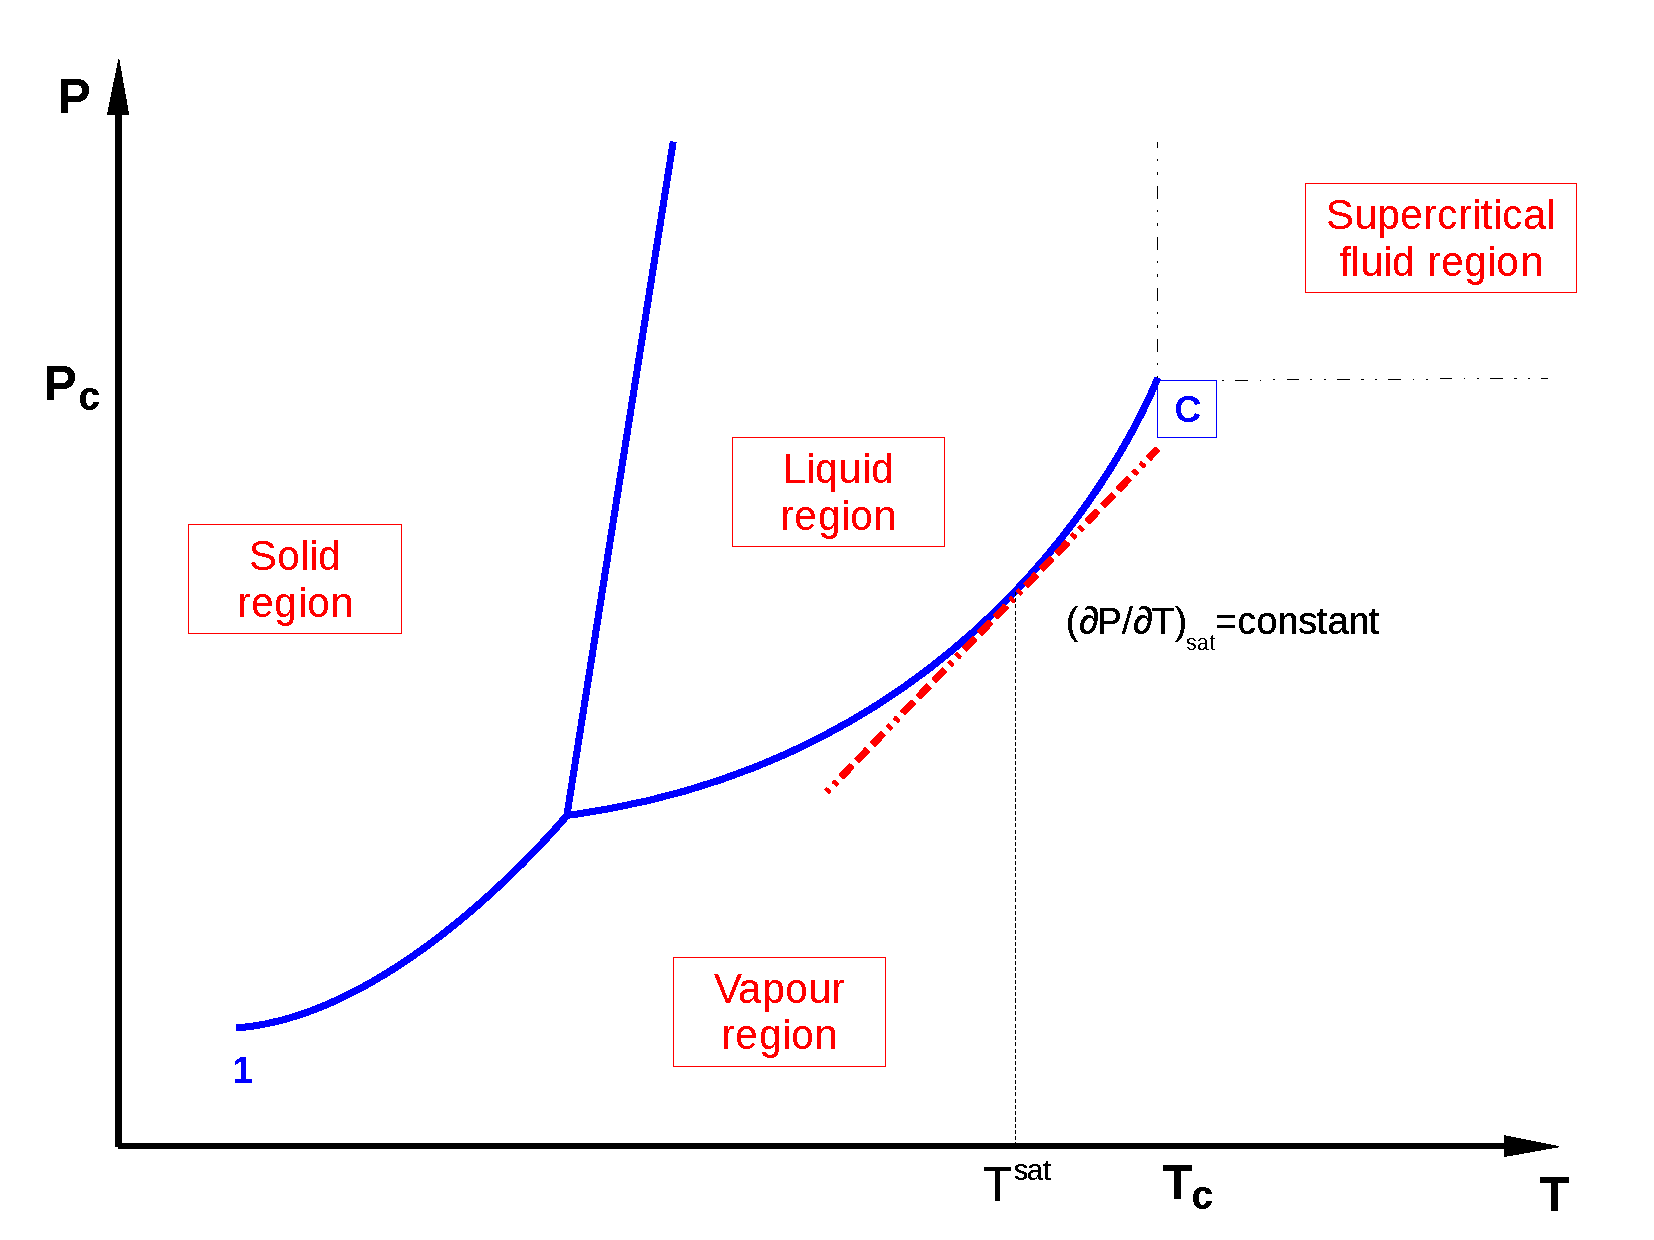
\includegraphics[width=.5\columnwidth,clip]{./../Pics/PT_Diagram2}
               \end{center} 
               \caption{ $PT$ diagrams for a pure substance. Graphical representation of the Clapeyron relation.}\label{Mod03Fig01}
           \end{figure}
      \begin{shaded}
          \begin{equation}
             \frc{d\left(\ln{P^{\text{sat}}}\right)}{dT} = \frc{\Delta H^{\text{fg}}}{RT^{2}} \;\;\Longrightarrow \;\;\; \ln{\left(\frc{P_{2}}{P_{1}}\right)_{\text{sat}}} = \frc{\Delta H^{\text{fg}}}{R}\left(\frc{1}{T_{1}}-\frc{1}{T_{2}}\right)_{\text{sat}}.\label{Mod03_ClausiusClapeyronEqn} 
          \end{equation} 
This expression is known as {\it Clausius-Clapeyron equation} and is a good approximation when describing temperature and pressure dependence at boiling/condensation and at sublimation/gas deposition.
      \end{shaded}
For the dependence of the saturated vapour pressure on $T$, a number of empirical relations have been developed. The simplest expression is,
    \begin{displaymath}
       \ln{P^{\text{sat}}} = A - \frc{B}{T},%\label{Mod03_AntoineSimplest}
    \end{displaymath}
where $A$ and $B$ are constants obtained from experiments. A more `popular' relation is,
    \begin{shaded}
       \begin{equation}
          \ln{P^{\text{sat}}} = A - \frc{B}{T+C},\label{Mod03_Antoine}
       \end{equation}
       this relation is known as {\it Antoine Equation}, where $A$, $B$ and $C$ are constants obtained experimentally.
    \end{shaded}
This two relations, although still widely used by the fluids community are plagued with strong inaccuracy. Due to better accuracy, high-order polynomial relations have become commonly used in flow and process simulators,
    \begin{displaymath}
       \ln{P^{\text{sat}}} = \frc{A\tau + B\tau^{1.5} + C\tau^{3} + D\tau^{6}}{1-\tau}\;\;\;\;\text{ with }\;\;\tau = 1 - T_{r}.
    \end{displaymath}
\end{subequations}


%%% SUBSECTION
   \subsection{Vapour-Liquid Equilibrium Systems}

Several processes of engineering relevance occur with fluids in phase equilibria -- either saturated vapour (\ie vapour saturated with liquid droplets) and saturated liquid (\ie liquid saturated with bubbles of vapour). In most cases, it is important to know the actual quantities of both phases in thermodynamic equilibrium, \ie the amount of vapour and liquid present in a constrained system at prescribed temperature and pressure conditions. Let assume that a closed system contains $n$ moles of a chemical species split into $\mathcal{P}$ phases,
    \begin{displaymath}
      n = \sum\limits_{j=1}^{\mathcal{P}} \mfr[n]{}{j} = \mfr[n]{}{1} + \mfr[n]{}{2} + \cdots + \mfr[n]{}{\mathcal{P}}.
    \end{displaymath}
The mass balance acroos all $\mathcal{P}$ phases can be represented as
    \begin{displaymath}
       nV = \mfr[n]{}{1}\mfr[V]{}{1} + \mfr[n]{}{2}\mfr[V]{}{2} + \cdots + \mfr[n]{}{\mathcal{P}}\mfr[V]{}{\mathcal{P}}  = \sum\limits_{j=1}^{\mathcal{P}}\left(nV\right)^{\left(j\right)},
    \end{displaymath}
where $V$ is the molar volume. Dividing by $n$
    \begin{displaymath}
       V = \frc{\mfr[n]{}{1}}{n}\mfr[V]{}{1} + \frc{\mfr[n]{}{2}}{n}\mfr[V]{}{2} + \cdots + \frc{\mfr[n]{}{\mathcal{P}}}{n}\mfr[V]{}{\mathcal{P}}.
    \end{displaymath}
Defining molar (or mole) fraction, $\mfr[x]{}{j}=\frc{\mfr[n]{}{j}}{n}$, where
    \begin{eqnarray}
         && \sum\limits_{j=1}^{\mathcal{P}}\mfr[x]{}{j} = 1,  \nonumber \\
         && V = \mfr[x]{}{1}\mfr[V]{}{1} + \mfr[x]{}{2}\mfr[V]{}{2} + \cdots + \mfr[x]{}{\mathcal{P}}\mfr[V]{}{\mathcal{P}}.  \nonumber
    \end{eqnarray}
For vapour-liquid systems,
    \begin{eqnarray}
         && \mfr[x]{}{L} + \mfr[x]{}{V} = 1,  \nonumber \\
         && V = \mfr[x]{}{L}\mfr[V]{}{L} + \mfr[x]{}{V}\mfr[V]{}{V}. \nonumber
    \end{eqnarray}
For a generic thermodynamic potential $M$ (= $V$, $U$, $H$, $S$ etc),
    \begin{shaded}
       \begin{subequations}
           \begin{equation}
              M = \left(1-\mfr[x]{}{V}\right)\mfr[M]{}{L} + \mfr[x]{}{V}\mfr[M]{}{V}
           \end{equation}
           \begin{equation}
              M = \mfr[M]{}{L} + \mfr[x]{}{V}\Delta\mfr[M]{}{LV}\label{Mod03_QualityVapour}
           \end{equation}
       \end{subequations}
    \end{shaded}
$\mfr[x]{}{V}$ is called \underline{\it vapour quality}. Thermodynamic potentials of pure substances are graphically represented by $Ph$ (pressure $\times$ specific enthalpy) and $Ts$ (temperature $\times$ specific entropy) diagrams, Fig.~\ref{Mod03Fig02}, where information on $P$, $T$, $s$, $h$, $x$ and $v$ (specific volume) can be readily extracted.
%
           \begin{figure}[h]
              \vbox{
                    \hbox{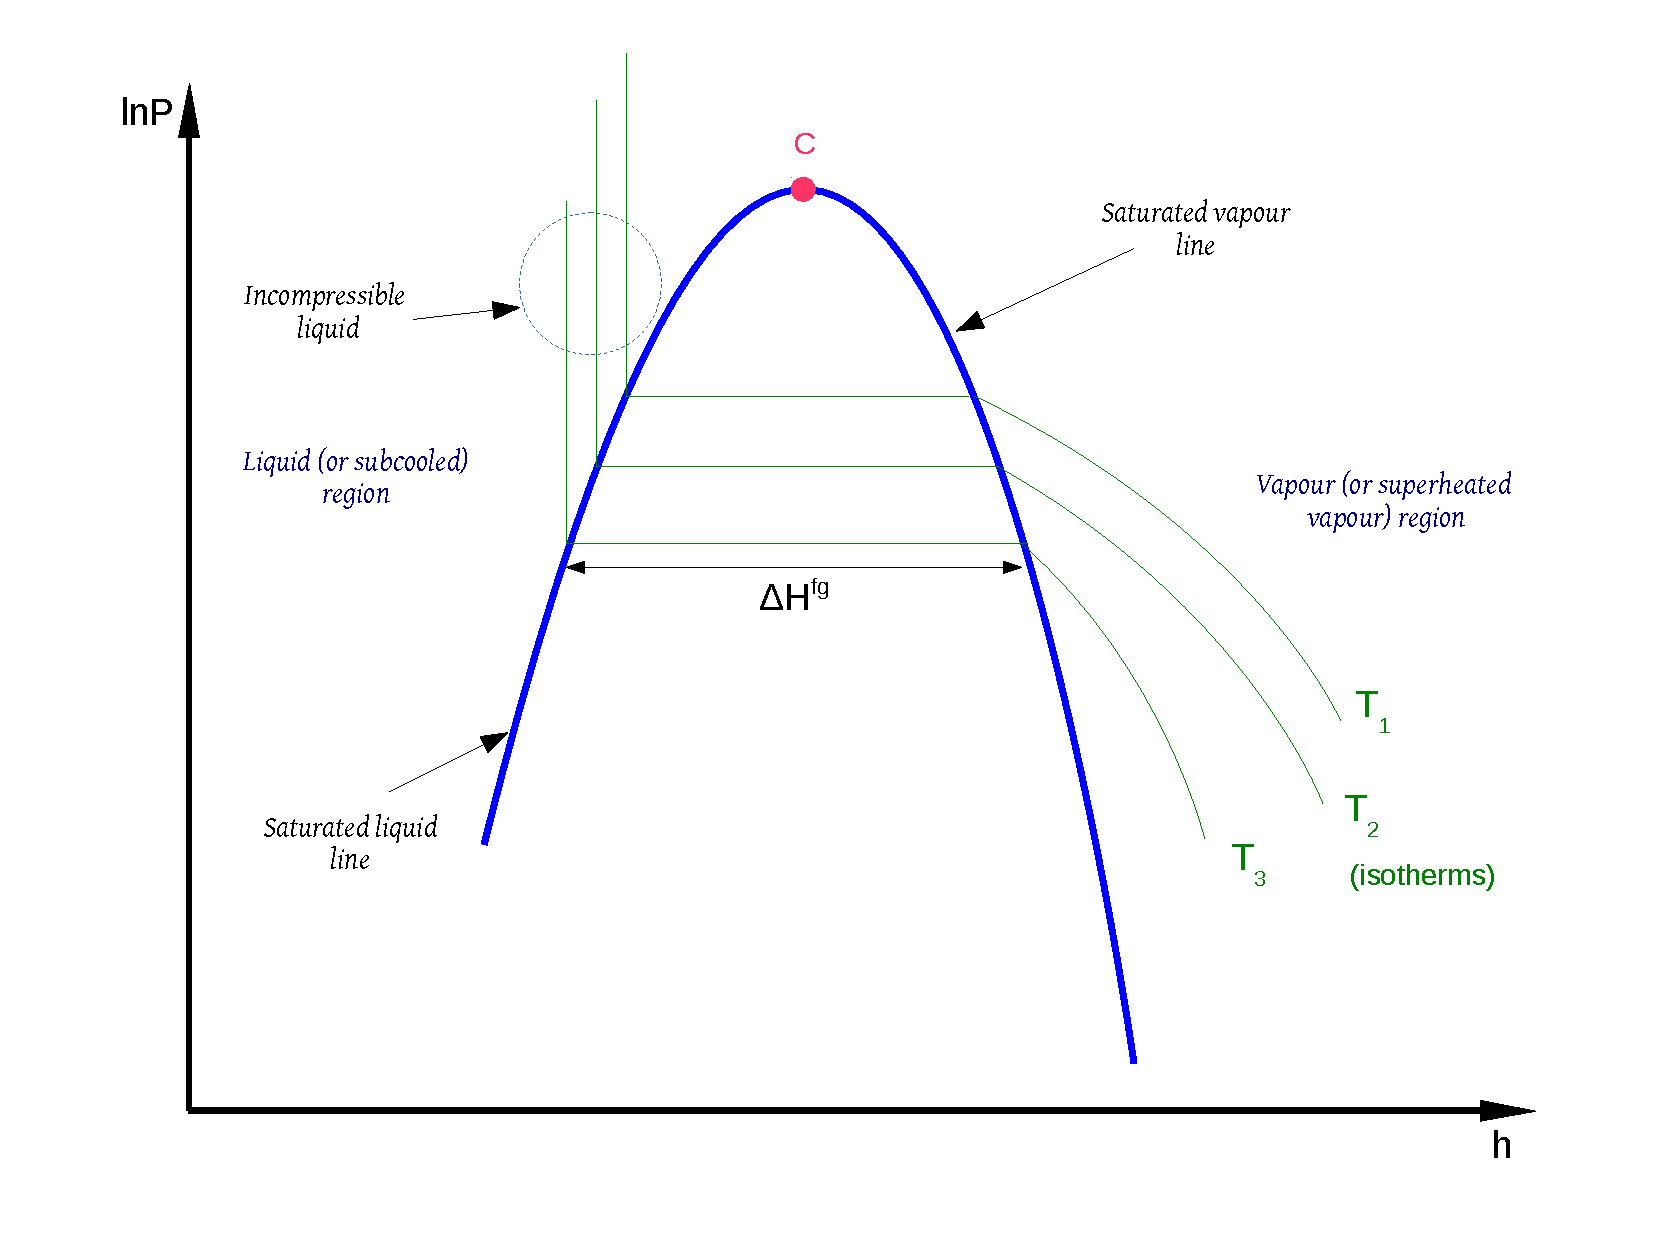
\includegraphics[width=.5\columnwidth,clip]{./Figs/Mod3PHDiagram}
                          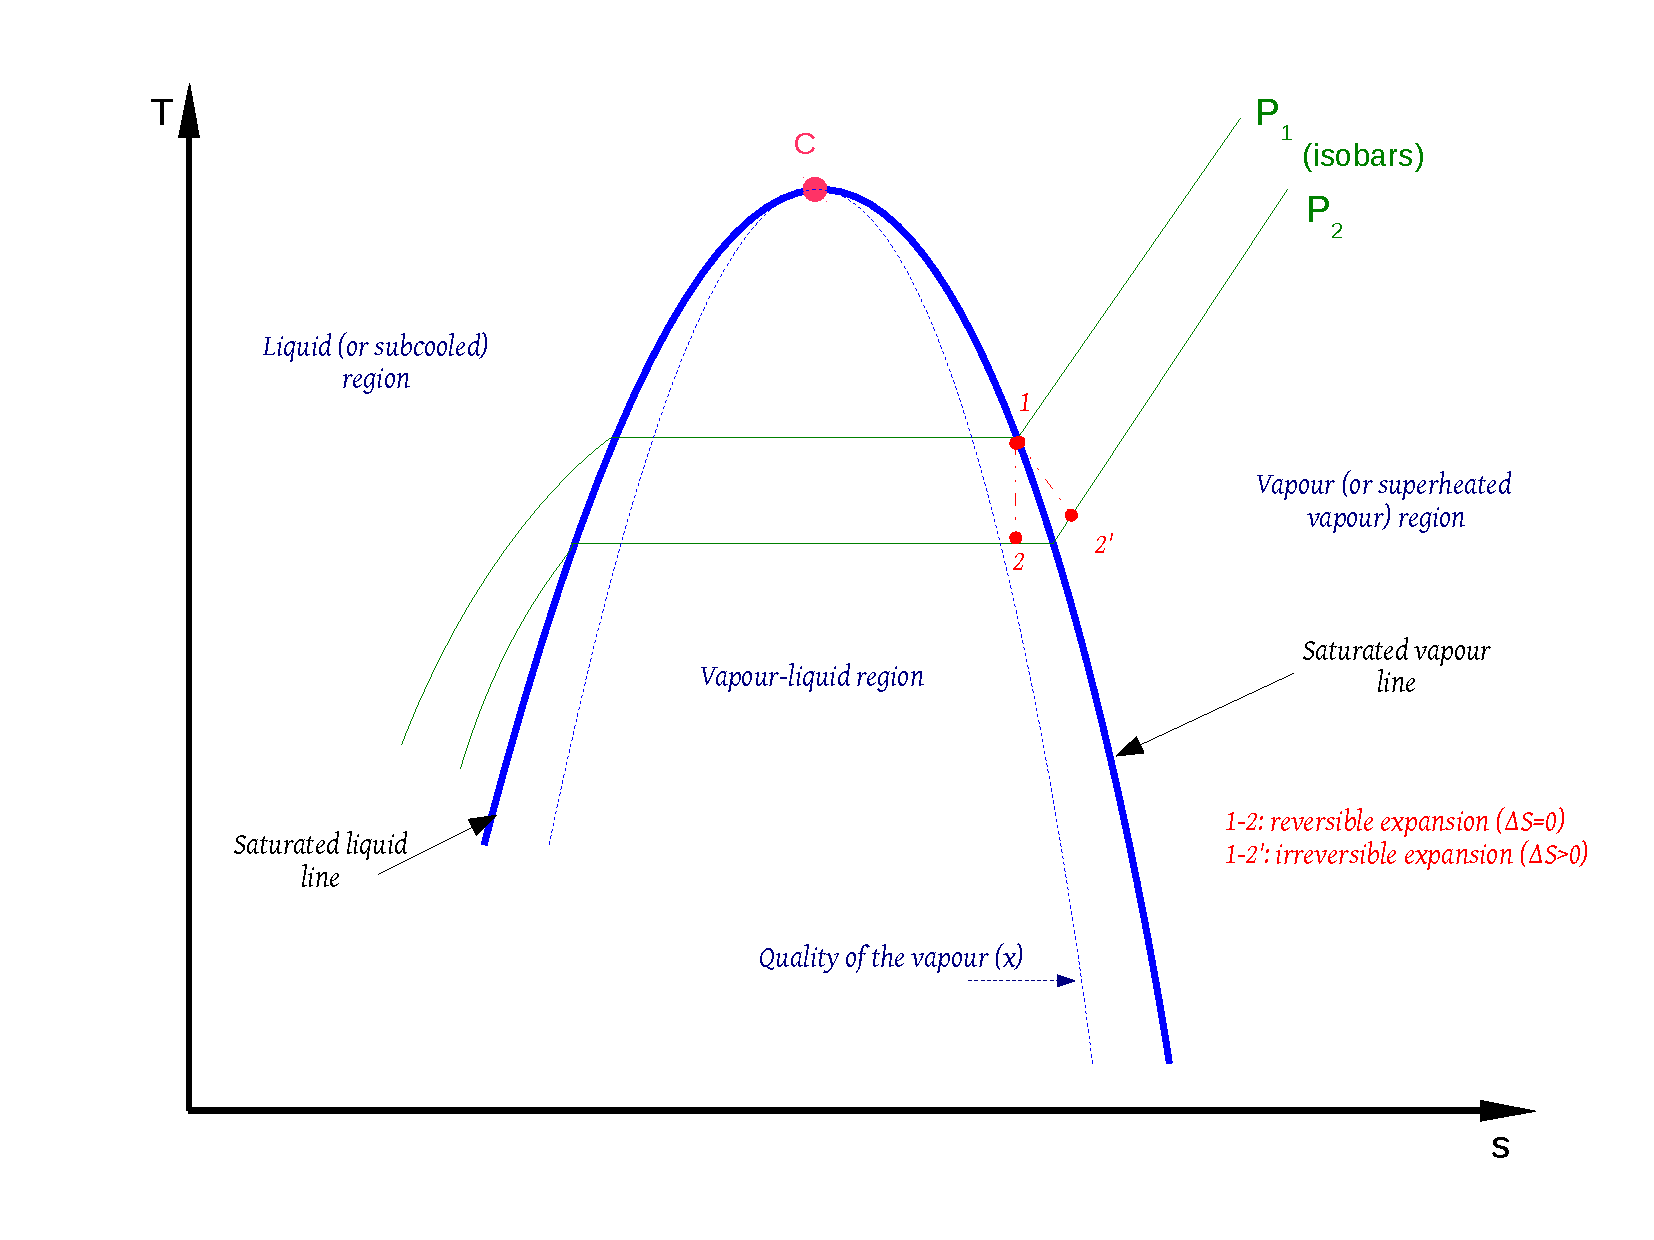
\includegraphics[width=.5\columnwidth,clip]{./Figs/Mod3TSDiagram}}
                    \vspace{-.1cm}
                    \hbox{\hspace{4cm}(a)\hspace{8cm}(b)}}
              \caption{ (a) $Ph$ and (b) $Ts$ diagrams for a pure substance.}\label{Mod03Fig02}
           \end{figure}
%
In the $Ph$ diagram, Fig~\ref{Mod03Fig02}a, isotherms (i.e., lines representing constant temperature) and pressure conditions determine the phase of the fluid. At the left hand-side of the {\it dome} all fluid is at liquid state, whereas at the right hand-side of the {\it dome}, all fluid is at vapour state. The region within the {\it dome} is a two-phase region, where liquid and vapour coexist in thermodynamic equilibrium. As the fluid conditions `move' from the {\it saturated liquid line} to the {\it saturated vapour line} through the {\it isotherm}, the fluid is continuously vaporised `till there is no droplets of liquid fluid. The total amount of heat given to the system -- $\Delta H^{\text{fg}}$, is the latent heat of vaporisation. In a similar way, the $Ts$ diagram, Fig~\ref{Mod03Fig02}b, shows similar features over different {\it isobars}. In addition, the {\it quality} of the vapour can also be graphically represented. In a reversible expansion from $P_{1}$ to $P_{2}$ $\left(P_{1}>P_{2}\right)$, entropy change is null, $\Delta s=0$, and is represented by a vertical line, however during irreversible expansion, $\Delta s >0$, represented by an inclined line.  

 $Ph$ and $Ts$ diagrams for common substances are no longer used by industry but it helps to qualitatively understand phase (and associated thermodynamic potentials) behaviour of pure substances. Quantitative information can be obtained from either saturated and superheated (Fig.~\ref{Mod03Fig03}) fluid tables or dedicated software, \eg
\begin{itemize}
   \item \href{http://www.weatherford.com/doc/wft183650}{PVTflex$^{TM}$};
   \item \href{http://www.kbcat.com/infochem-software/flow-assurance-software-multiflash/pvt-simulation}{Multiflash$^{TM}$};
   \item \href{https://www.honeywellprocess.com/en-US/explore/products/advanced-applications/unisim/Pages/default.aspx}{UniSim – Software for Process Design and Simulation};
   \item \href{http://webbook.nist.gov/chemistry/fluid/}{NIST Website}
   \item etc.
\end{itemize}
In general, table of {\it saturated fluid properties}, Fig.~\ref{Mod03Fig03}a, contains information of the fluid within the {\it dome}, whereas the table of {\it superheated fluid properties} refer to the region outside (rhs) the {\it dome}. 
%
   \begin{figure}[h]
      \vbox{
         \hbox{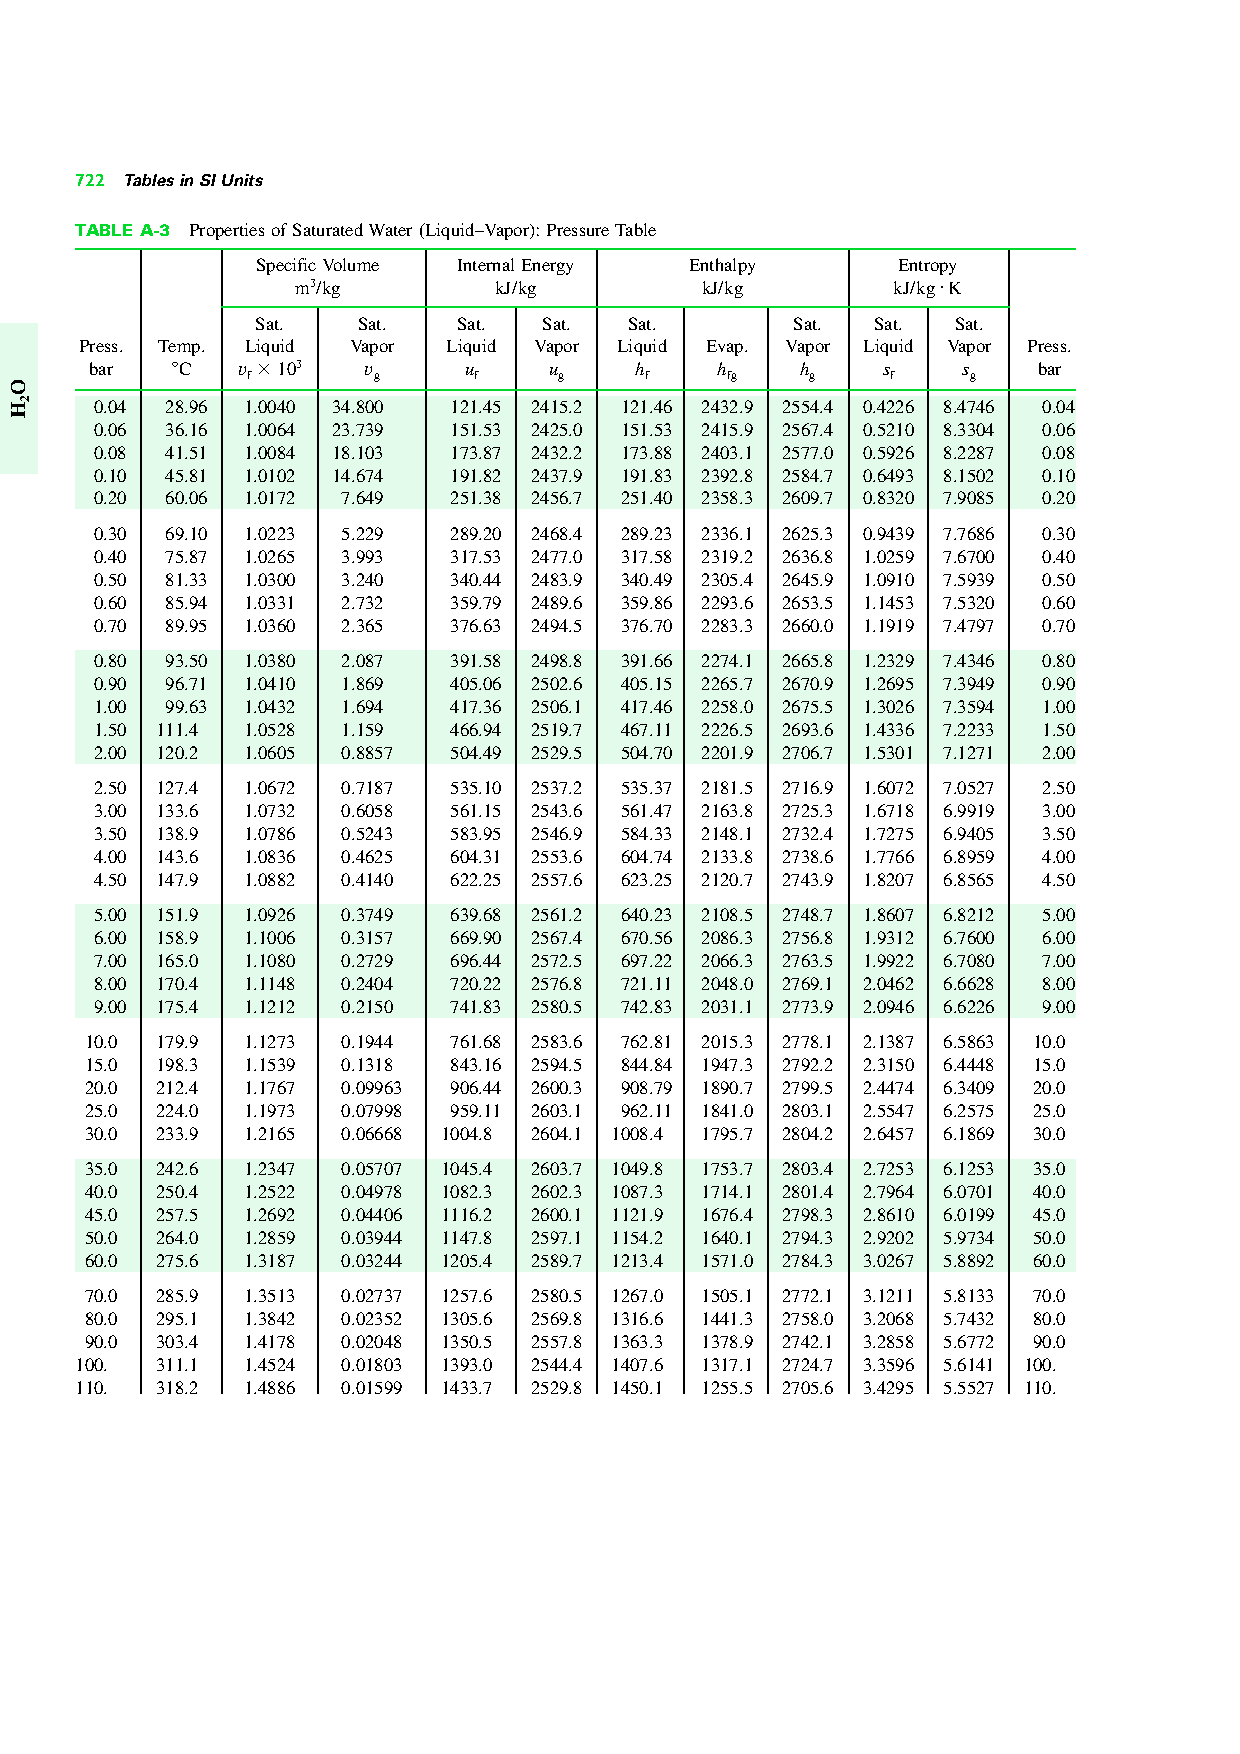
\includegraphics[width=.5\columnwidth,clip]{./Figs/WaterSatTable}
               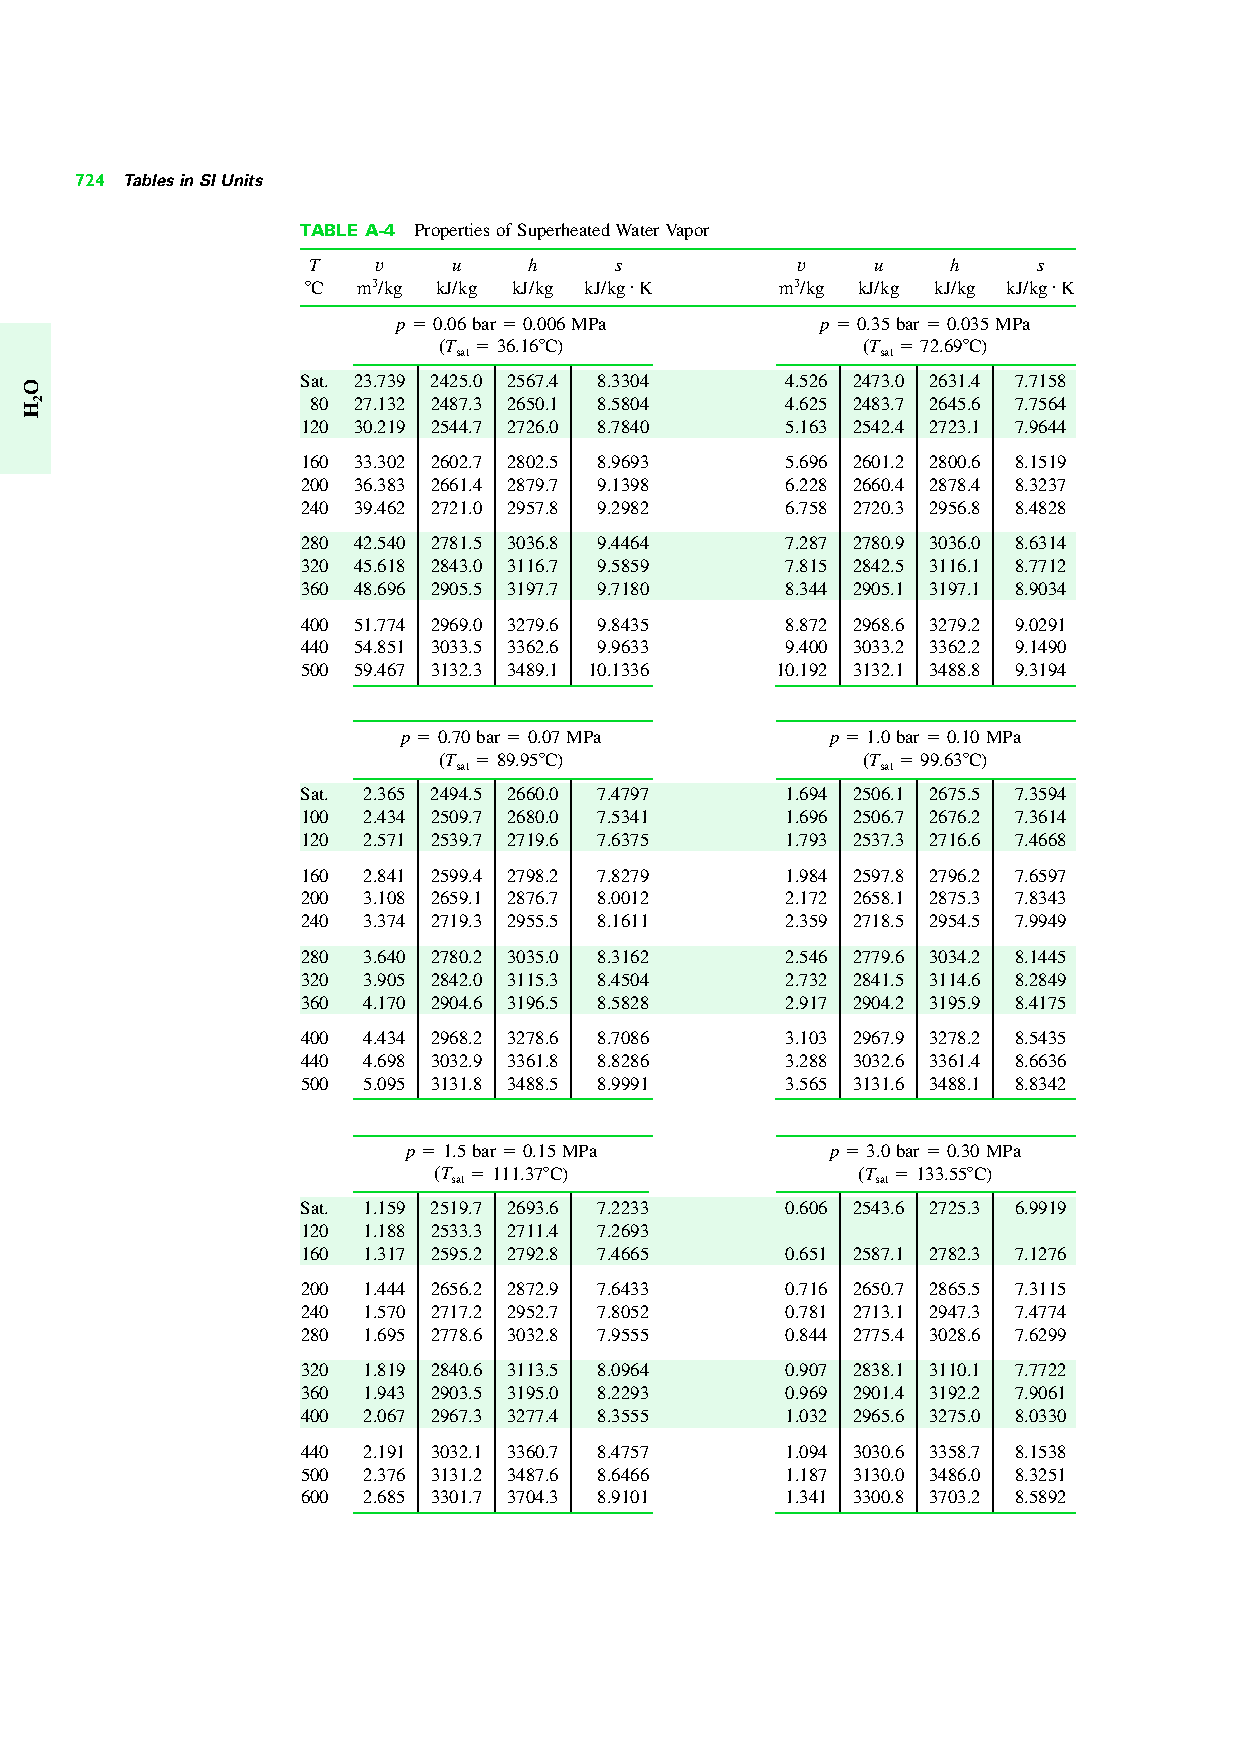
\includegraphics[width=.5\columnwidth,clip]{./Figs/Water_SuperheatedTable}}
         \vspace{-1.5cm}
         \hbox{\hspace{4cm}(a)\hspace{7cm}(b)}
      }
      \caption{ Table of properties of (a) saturated water-steam and (b) superheated vapour (Extracted from Moran $\&$ Saphiro, see Appendix B).}\label{Mod03Fig03}  
   \end{figure}
%
    

%%% SUBSECTION
   \subsection{Industrial Applications: Power System}
Regardless the energy source (fossil fuel, nuclear or geothermal), power plants are good applications for VLE systems as fluids are continuously vaporised and condensed by addition and extraction of heat and volume expansion. {\it Rankine thermal cycles} are system configurations for generating power and consist of four processes (Fig.~\ref{Mod03Fig04}) with associated energy balances:
     \begin{itemize}
      \item \textcolor{red}{Process 1-2}: reversible adiabatic (i.e., \blue{isentropic}) expansion in the turbine (or steam engine),
            \begin{displaymath}
               \left(h_{2} + \dot{W}_{T}\right)-h_{1} = 0 \Rightarrow \dot{W}_{T} = h_{1}-h_{2}
            \end{displaymath}
      \item \textcolor{red}{Process 2-3}: constant-pressure heat transfer (to the environment) in the condenser,
            \begin{displaymath}
               \left(h_{3} + \dot{Q}_{C}\right)-h_{2} = 0 \Rightarrow \dot{Q}_{C} = h_{2}-h_{3}
            \end{displaymath}
      \item \textcolor{red}{Process 3-4}: reversible adiabatic (i.e., \blue{isentropic}) pumping process in the feed pump,
            \begin{displaymath}
               h_{4} - \left(h_{3} + \dot{W}_{P}\right) = 0 \Rightarrow \dot{W}_{P} = h_{4}-h_{3}
            \end{displaymath}
      \item \textcolor{red}{Process 4-1}: constant-pressure heat transfer (to the fluid) in the boiler,
            \begin{displaymath}
               h_{1} - \left(h_{4} + \dot{Q}_{B}\right) = 0 \Rightarrow \dot{Q}_{B} = h_{1}-h_{4}
            \end{displaymath} 
     \end{itemize}
     The efficiency $\left(\eta\right)$ of the Rankine cycle is given by
           \begin{displaymath}
               \eta_{\text{Rankine}} = \frc{\sum W_{i}}{Q_{B}} = \frc{\left|W_{\text{net}}\right|}{Q_{B}} = \frc{\left|\left(h_{1}-h_{2}\right)+\left(h_{4}-h_{3}\right)\right|}{h_{1}-h_{4}}.
           \end{displaymath}
     Due to engineering constraints, fluids entering and leaving the pump \underline{must be} at liquid phase, thus $h_{4}=h_{f4}$ and $h_{3}=h_{f3}$, \ie the fluid has the enthalpy of the liquid phase (from the saturated fluid table) at the prescribed temperature and pressure conditions. {\it Pumps} are able to induce the transport of liquid fluids that are often assumed incompressible, therefore
          \begin{displaymath}
                Tds = dh - v dP
          \end{displaymath}
as the compression occurs isentropically, \ie $ds=0$,
          \begin{displaymath}
                dh = v dP \Rightarrow h_{f4} = h_{f3} + v_{3}\left(P_{4}-P_{3}\right).
          \end{displaymath}
However, as $\left(h_{f4}-h_{f3}\right) <<<<< \left(h_{1}-h_{2}\right)$, the efficiency can be considered as
           \begin{displaymath}
               \eta_{\text{Rankine}} = \frc{\left|\left(h_{1}-h_{2}\right)\right|}{h_{1}-h_{f4}}.
           \end{displaymath}     
%
   \begin{figure}[h]
      \begin{center}
         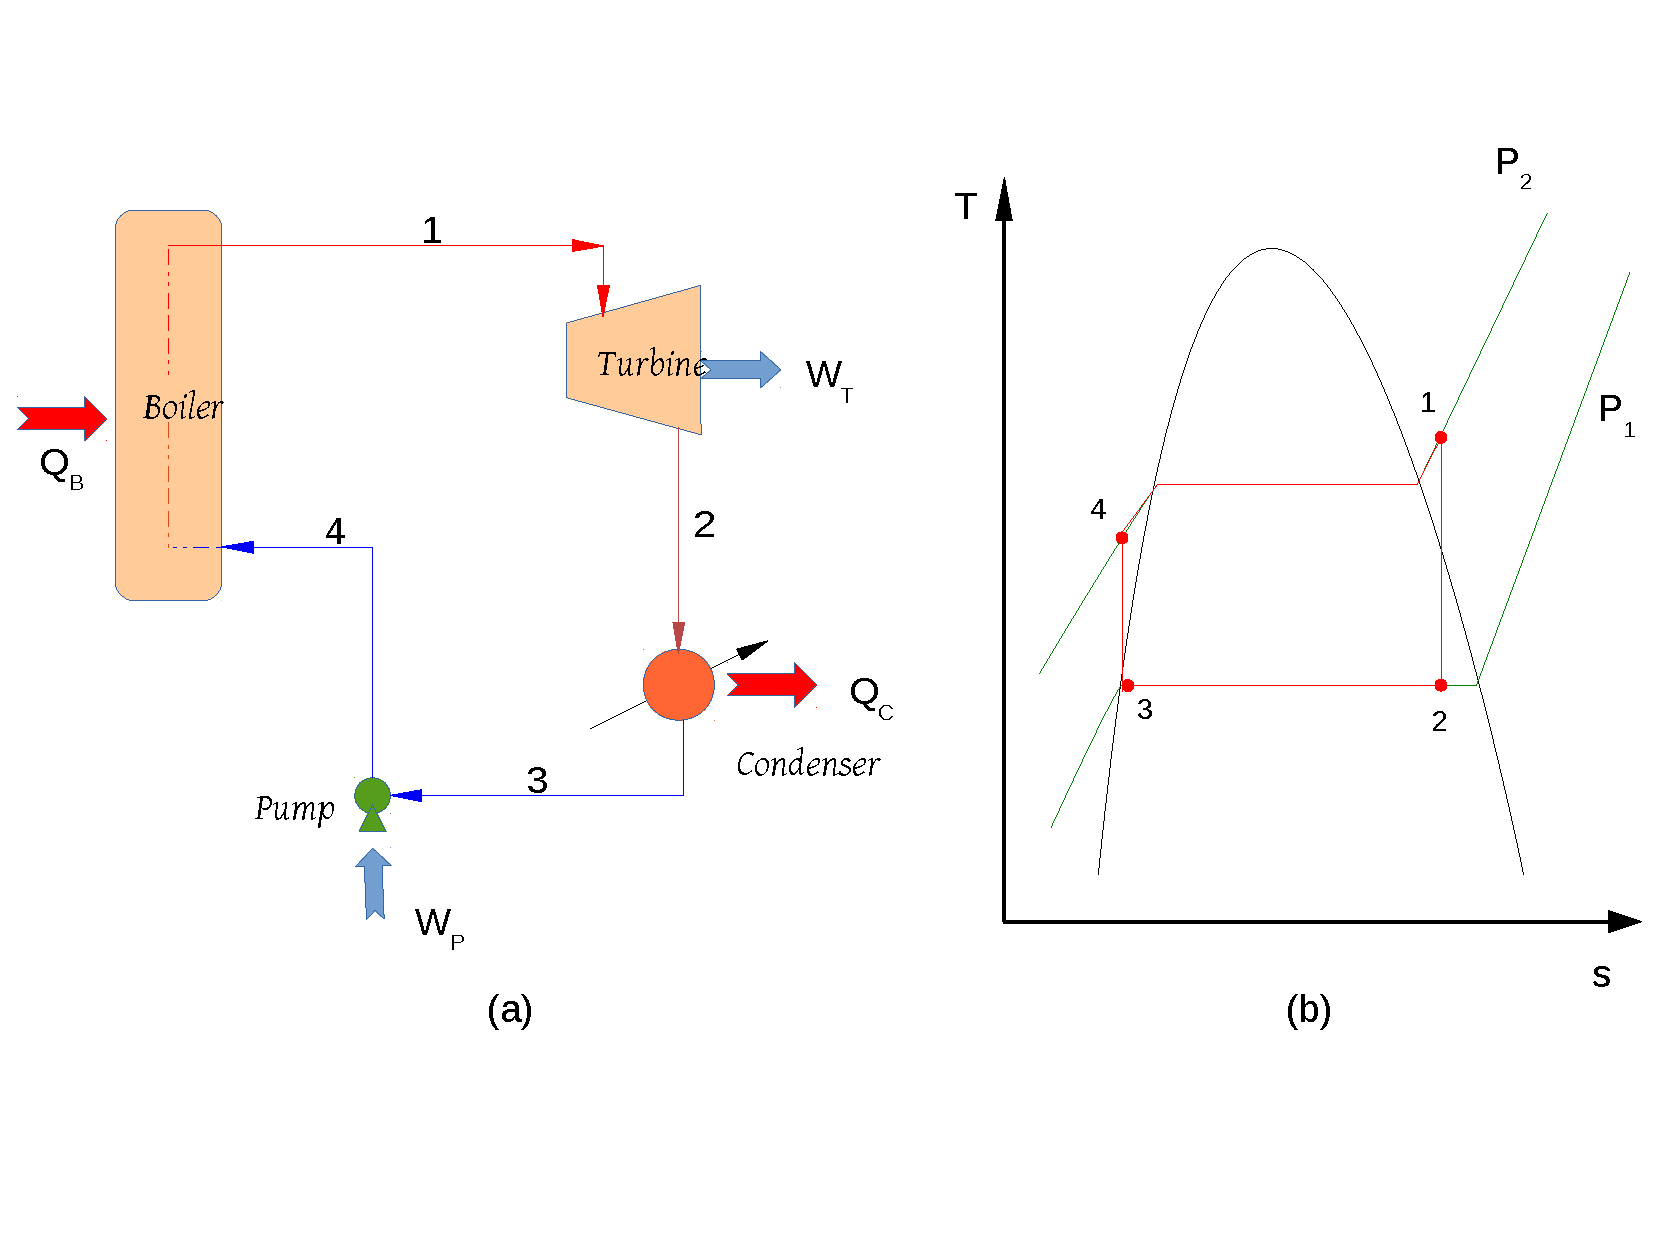
\includegraphics[width=\columnwidth,clip]{./Figs/Mod3PowerSystemDiagram}
      \end{center}
      \caption{ (a) Diagram of Rankine thermal cycle for power generation and associated $Ts$ diagram.}\label{Mod03Fig04}
   \end{figure}


\clearpage

%%% SECTION
\section{Examples}
       \begin{enumerate}

%%%
%%% EXAMPLE 
%%%
\item\label{Mod03Ex03} The Antoine equation constants for toluene are $A=14.01415$, $B=3106.46$ K and $C=-53.15$ K (for pressure given in kPa). At 1.01325$\times$10$^{5}$ Pa, calculate the boiling temperature and the enthalpy of vaporisation at this temperature.

% SOLUTION
    \noindent{\bf Solution:} Boiling temperature can be calculated from the Antoine equation,
       \begin{displaymath}
          \ln{P^{\text{sat}}} = A - \frc{B}{T+C} \;\;\;\Rightarrow \;\;\; T = \frc{B}{A-\ln{P^{\text{sat}}}} - C = \red{383.77 K}
       \end{displaymath}
The enthalpy of vaporisation, $\Delta H^{\text{fg}}$, can be obtained from the Clausius-Clapeyron equation,
         \begin{eqnarray}
            \frc{d}{dT} \left(\ln{P^{\text{sat}}}\right) &=& \frc{\Delta H^{\text{fg}}}{RT^{2}} \nonumber \\
             \frc{B}{\left(T+C\right)^{2}} &=&  \frc{\Delta H^{\text{fg}}}{RT^{2}} \;\;\Longrightarrow \Delta H^{\text{fg}} = 34.7984 \text{kJ.mol}^{-1}. \nonumber
         \end{eqnarray}
 
\clearpage

%%%
%%% EXAMPLE 
%%%  
\item\label{Mod03Ex04} Derive an expression for enthalpy change of a gas during an isothermal process assuming using the following EOS: $P\left(V-b\right)=RT$

% SOLUTION
    \noindent{\bf Solution:} We have seen that enthalpy change is given by Eqn.~\ref{Chapter:ThermodynamicPropertiesPureFluids:Eqn:DerivedEnthalpyRelation1},
    \begin{displaymath}
       dH = C_{p}dT + \left[V - T\Partial[V]{T}{P}\right]dP.
    \end{displaymath}
    We can rearrange the given EOS and obtain $\Partial[V]{T}{P}$,
    \begin{eqnarray}
       && P\left(V-b\right)=RT \;\;\;\rightarrow\;\;\; V = \frc{RT}{P} + b \;\;\;\rightarrow\;\;\; \Partial[V]{T}{P} = \frc{R}{P}\;\;\text{ thus, } \nonumber \\
       && dH = C_{p}dT + \left(V - \frc{RT}{P}\right)dP = \blue{C_{p}dT + bdP}. \nonumber 
    \end{eqnarray}
    
\clearpage
    
\clearpage
 
%%%
%%% EXAMPLE 
%%%  
\item\label{Mod03Ex06} Steam (dry and saturated) is supplied by the boiler at 15 bar and the condenser inlet pressure is 0.4 bar. Calculate the Rankine efficiency of the cycle. Neglect the pump work, assume the enthalpy of fluid leaving the pump is 317.58 kJ.kg$^{-1}$

% SOLUTION  
    \noindent{\bf Solution:} At 15 bar, dry and saturated $\left(\ie x_{1}=1\right)$ steam has the following properties (from saturated table)\footnote{Using the same numbering as in Fig.~\ref{Mod03Fig04}.},
          \begin{eqnarray}
             T_{1} &=& T_{\text{sat}} = 198.3^{\circ}\text{C},\nonumber \\
             h_{1} &=& h_{\text{g}} = 2792.2\; \text{kJ.kg}^{-1} \nonumber \\
             s_{1} &=& s_{\text{g}} = 6.4448\; \text{kJ.(kg.K)}^{-1} \nonumber
          \end{eqnarray} 
    In the condenser, $P_{2}=0.4$ bar,
          \begin{eqnarray}
              T_{2} &=& T_{\text{sat}} = 75.87^{\circ}\text{C}, \nonumber \\
              h_{\text{g}2} &=& 2636.8\;\text{kJ.kg}^{-1},\;\;\; h_{\text{f}2} = 317.58\;\text{kJ.kg}^{-1},  \nonumber \\
              s_{\text{g}2} &=& 7.6700 \;\text{kJ.(kg.K)}^{-1},\;\;\; s_{\text{f}2} = 1.0259\;\text{kJ.(kg.K)}^{-1}. \nonumber  
          \end{eqnarray}
$h_{2}$ and $s_{2}$ depend on the knowledge of how vaporised the water is, in other words, we need to determine the quality of the steam, $x_{1}$ through Eqn.~\ref{Mod03_QualityVapour},
      \begin{eqnarray}
          h_{2} &=& h_{\text{f}2} + x_{2}\left(h_{\text{g}2} - h_{\text{f}2}\right), \nonumber \\
          s_{2} &=& s_{\text{f}2} + x_{2}\left(s_{\text{g}2} - s_{\text{f}2}\right). \nonumber
      \end{eqnarray}
As we know that water is expanded isentropically in the turbine, \ie $s_{1}=s_{2}$,
      \begin{displaymath}
         s_{2} = s_{\text{f}2} + x_{2}\left(s_{\text{g}2} - s_{\text{f}2}\right) = s_{1} = 6.4448 \;\;\;\Rightarrow \;\;\; x_{2} = 0.8156 \;\;(81.56\% \text{ of vapour}
      \end{displaymath}
Thus replacing in 
      \begin{displaymath}
          h_{2} = h_{\text{f}2} + x_{2}\left(h_{\text{g}2} - h_{\text{f}2}\right) = 2209.14\text{ kJ.kg}^{-1}.
      \end{displaymath}
The Rankine efficiency is given by
      \begin{displaymath}
           \eta_{\text{Rankine}} = \frc{\text{Adiabatic or Isentropic Heat Drop}}{\text{Heat Supplied}} = \frc{\left|h_{1}-h_{2}\right|}{h_{1}-h_{\text{f}4}} = 0.2356\;\;\;\rightarrow \;\;\; 23.56\%
      \end{displaymath}
    


\end{enumerate}


 % Thermodynamic Properties of Pure Fluids
     \setcounter{examplecounter}{0}
  \chapter{Vapour-Liquid Equilibrium of Mixtures}\label{Chapter:VLE}


   \begin{LearningObjectivesBlock}{Learning Objectives}
      Upon completion of this chapter, you will be able to
        \begin{enumerate}
           \item Assess properties of real fluids through excess properties definitions; 
           \item Define phase and components molar fractions;
           \item Discuss chemical potential as a critical element for chemical equilibrium;
           \item Determine conditions for chemical equilibrium;
           \item Estimate phases, compositions and thermodynamic potentials in 2-/3-D phase diagrams;
           \item Identify and calculate bubble and dew points coordinates (\ie pressure, temperature and compositions);
           \item State Raoult's and Henry's laws;
           \item Formulate mass balance for VLE problems and estimate compositions at equilibrium.
        \end{enumerate}
\medskip
     Recommended reading: Chapters 10-11 of \citet{SmithVanNess_Book}, 8-10 of \cite{Sandler_Book}, 3-5 of \citet{Lue_Book}, 11 of \citet{Moran_Book} or 4-7 of \citet{Atkins_Book}.
   \end{LearningObjectivesBlock}


%%%%%%%%%%%%%%%%%%%%%%%%%%%%%%%%%%%%%%%%%%%%%%%%%%%%%%%%%%%%%%%%%
\begin{comment}
   \begin{LearningObjectivesBlock}{Learning Objectives}
      Upon completion of this chapter, you will be able to
        \begin{enumerate}
           \item {\bf Knowledge:} Define, Name, Select, State 
           \item {\bf Comprehension:} Describe, Identify, Discuss
           \item {\bf Application:} Apply, Demonstrate, Employ, Sketch
           \item {\bf Analysis:} Analyse, Compare, Calculate, Solve
           \item {\bf Synthesis:} Determine, Formulate
           \item {\bf Evaluation:} Assess, Check, Estimate, Compare, Measure, Monitor
        \end{enumerate}
\end{comment}
%%%%%%%%%%%%%%%%%%%%%%%%%%%%%%%%%%%%%%%%%%%%%%%%%%%%%%%%%%%%%%%%%

%%%% ETOC
\localtableofcontents
   

%%% SECTION
\section{Introduction}\label{Chapter:VLE:Section:Introduction}
Up to this point, we have only considered thermodynamic and volumetric properties of pure components at prescribed pressure and temperature conditions. However, most engineering applications deals with mixtures of components that may be present in single or multiple phases, \eg oil in reservoirs, naphtha distillation, steel processing etc. This chapter focuses on understanding PVT behaviour of mixtures and the conditions for vapour-liquid equilibrium (VLE).



%%% SECTION
\section{A Few Important Definitions}
In the previous chapters, we mostly focused on thermodynamic properties of systems containing pure chemical species. This chapter (and the remaining of this notes) will study systems with arbitrary number of components, and the quantification of each component at each phase (Gibbs phase rule, Section~\ref{Chapter:VolumetricPropertiesPureSubstances:Section:GibbsPhaseRule}, is fundamental to determine the number of degrees of freedom in two-phase system with arbitrary number of chemical species).\index{Phase rule}

%%% SUBSECTION
\subsection{Representing Compositions}\label{Chapter:VLE:Section:Compositions}
 For a mixture containing $\mathcal{C}$ chemical species, each of them with an arbitrary number of moles, $n_{i},\;\;\forall i\in\left\{1,2,\cdots,\mathcal{C}\right\}$,
\begin{subequations}
   \begin{enumerate}[a)]\index{Molar fraction}
       \item Molar (or mole) fraction $\left(x_{i}\right)$:
            \begin{eqnarray}
                x_{i} = \frc{n_{i}}{n},\label{Chapter:VLE:Eqn:MolarFraction}
            \end{eqnarray} 
            where $n=\summation[n_{i}]{i=1}{\mathcal{C}}$ is the total number of moles in the system. As the molar fraction is a normalised quantity, the following constraint is imposed:
            \begin{equation}
                  \summation[x_{i}]{i=1}{\mathcal{C}} = 1,\label{Chapter:VLE:Eqn:MolarFractionConstraint}
            \end{equation}
       \item (Average) Molar mass of mixtures:\index{Molar mass}\index{Molar weight|see {Molar mass}}
            \begin{equation}
                \overline{MW} = \summation[\left(x_{i} \cdot MW_{i}\right)]{i=1}{\mathcal{C}}\label{Chapter:VLE:Eqn:MolarMass}
            \end{equation}
         where $MW_{i}$ is the molecular mass (or molar weight) of species $i$;
       \item Molality of a solution ($\mathcal{M}$) is defined as the concentration (as number of moles) of the solute in 1 kg of solvent,
            \begin{equation}
                  \mathcal{M} = \frc{n_{i}}{m_{s}}=\frc{n_{i}}{n_{s}MW_{s}},\label{Chapter:VLE:Eqn:Molality}
            \end{equation}
   \end{enumerate}
\end{subequations}

%%% SUBSECTION
\subsection{Partial Molar Properties}\label{Chapter:VLE:Section:PartialMolarProperties}\index{Partial molar properties}
Many thermodynamic properties of {\it ideal solutions} do not change on mixing, for example, the volume of a mixture (assumed ideal) is equal to the sum of the volume of the original unmixed solutions. However, in real systems the volume and other properties, are not additive, \ie the volume of a mixture is not equal to the sum of the volumes of the individual pure components. {\it Partial molar properties} describe the behaviour of homogeneous multi-component systems. Thus, the concept of partial molar properties are crucial tool to assess individual contribution to thermodynamic properties of mixtures. In Section~\ref{Chapter:SolutionThermodynamics:Section:GibbsDuhem}, an expression will be developed to assess thermodynamic properties of solutions based on this concept. 

 Let's consider a homogeneous (\ie single phase) and open system with $\mathcal{C}$ chemical species that undertakes a change in composition. Thus, the total value of any extensive property $M^{\text{t}}\;\left(M\equiv V, U, H, S, G, A\right)$ is not only a function of pressure and temperature, but it also depends on the number of moles of each species in the system, therefore
  \begin{subequations}
     \begin{equation}
       M^{\text{t}} = nM = M\left(T,P,n_{1},n_{2},\cdots, n_{\mathcal{C}}\right).\label{Chapter:VLE:Eqn:PartialProperties1}
     \end{equation}
     The total derivative of this property, $M^{\text{t}}$, is,
     \begin{displaymath}  
        d(nM) = \Partial[(nM)]{P}{T,n}dP + \Partial[(nM)]{T}{P,n}dT + \Partial[(nM)]{n_{i}}{T,P,n_{j\ne i}}dn_{i},
     \end{displaymath}
     where the subscript $n$ in the partial derivatives indicates that the number of moles is kept constant, whereas $n_{j\ne i}$ indicates that the number of moles of all components, except component $i$, are kept constant. This expression can be simplified to be a function of the mole fraction, $x_{i}$,
     \begin{shaded}
        \begin{equation}  
           d(nM) = n\Partial[M]{P}{T,x}dP + n\Partial[M]{T}{P,x}dT + \summation[\overline{M}_{i}dn_{i}]{i}{},\label{Chapter:VLE:Eqn:PartialProperties2}
        \end{equation}
        where
        \begin{displaymath}
          \overline{M}_{i} = \Partial[(nM)]{n_{i}}{T,P,n_{j\ne i}},
        \end{displaymath}
        defines the {\it partial molar property} of species $i$ in solution, \ie the change of the total property $M^{\text{t}}$ of a mixture of $\mathcal{C}$ species resulting from the addition at constant $T$ and $P$ of infinitesimal amount of species $i$ to a prescribed amount of solution. We will discuss applications of partial molar properties in Chapter~\ref{Chapter:SolutionThermodynamics}.
     \end{shaded}
  \end{subequations}

%%% SUBSECTION
\subsection{Excess Properties}\label{Chapter:VLE:Section:ExcessProperties}\index{Excess properties|see {Solutions}}\index{Solutions!Excess properties}
  
In Section~\ref{Chapter:ThermodynamicPropertiesPureFluids:Section:ResidualProperties}, {\it residual properties} were defined as the difference between any extensive thermodynamic property, $M$, in real gases and its equivalent assuming ideal gas behaviour, $M^{\text{ig}}$. This entity is only applied to gases, an equivalent for liquids is called {\it excess properties}, \ie the deviation from an ideal liquid solution property\footnote{A formal definition of ideal solutions will be seen in Section~\ref{Chapter:SolutionThermodynamics:Section:IdealSolution}.}.\index{Gases!Residual properties}\

Let's assume that $M$ is any extensive thermodynamic property (\eg $V$, $U$, $H$, $S$, $G$ and $A$), the excess property $M^{\text{E}}$ is defined as the difference between the property value of a solution and the value it would have as an ideal solution at the same $T$, $P$ and composition,
\begin{subequations}
  \begin{shaded}
    \begin{equation}
       M^{\text{E}} \equiv M - M^{\text{id}},\label{Chapter:VLE:Eqn:ExcessProperties1a}
    \end{equation}
  \end{shaded}
  \noindent where properties in ideal ({\it id}) solutions of multiple chemical species can be represented as,
    \begin{displaymath}
       M^{\text{id}} = \summation[x_{i}M_{i}]{i}{},
    \end{displaymath}
    where $M_{i}$ is an extensive molar property of the \underline{pure} chemical species. For example, if we mix equal volumes of two species (\eg water and ethanol), the final volume \underline{is not} the sum of the individual volumes. In fact, the final volume will be slightly larger than the sum of the individual volumes and this is due to the non-ideality behaviour of real liquid fluids. Thus for a binary solution ($\mathcal{C}=$ 2),
    \begin{shaded}
      \begin{equation}
        V^{\text{E}} = V - V^{\text{id}} = V - \summation[x_{i}V_{i}]{i}{} = V -\left(x_{1}V_{1}+x_{2}V_{2}\right).\label{Chapter:VLE:Eqn:ExcessProperties1b} 
      \end{equation}
      This equation shows that the total volume of a mixture of two components is different from the simple addition of both individual volumes.
    \end{shaded}
\end{subequations}
  
%%% SECTION
\section{Chemical Potential $\left(\mu_{i}\right)$}\label{Chapter:VLE:Section:ChemicalPotential}\index{Chemical potential}
  \begin{subequations}
If we apply the concept of partial molar property to the Gibbs free energy definition, assuming that this thermodynamic potential is a function of $P$, $T$ and $n$, \ie $G^{\text{t}}= nG = G\left(T,P,n_{1},n_{2},\cdots,n_{\mathcal{C}}\right)$,
      \begin{equation}
         d(nG) = n\Partial[G]{P}{T,x}dP + n\Partial[G]{T}{P,x}dT + \summation[\overline{G}_{i}dn_{i}]{i}{}.\label{Chapter:VLE:Eqn:ChemPotentialDef1}
      \end{equation}
      By definition the {\it partial molar Gibbs free energy} is called chemical potential $\left(\mu_{i}\right)$,
      \begin{shaded}
         \begin{equation}
            \overline{G}_{i} = \mu_{i} = \Partial[(nG)]{n_{i}}{T,P,n_{j\ne i}}. \label{Chapter:VLE:Eqn:ChemPotentialDef1b}
         \end{equation}
      \end{shaded}
      The chemical potential can be understood as an energy associated with interactions of atoms/molecules in a mixture that controls the tendency of molecules to either leave the liquid solution (towards the vapour phase) or return to the solution (from the vapour phase) to vapour phase, and to chemically react. The Gibbs free energy was defined in Eqn.~\ref{Chapter:ThermodynamicPropertiesPureFluids:Eqn:GibbsFundamentalRelation01} as a function of $T$ and $P$, now it can be extended to be also a function of the number of moles of the existing chemical species, and Eqn.~\ref{Chapter:VLE:Eqn:ChemPotentialDef1} becomes,
      \begin{equation}
         d(nG) = (nV)dP - (nS)dT + \summation[\mu_{i}dn_{i}]{i}{},\label{Chapter:VLE:Eqn:ChemPotentialDef1c}
      \end{equation}
      using Eqns.~\ref{Chapter:ThermodynamicPropertiesPureFluids:Eqn:MaxwellRelation7}-\ref{Chapter:ThermodynamicPropertiesPureFluids:Eqn:MaxwellRelation8}. Now, assuming $n=1\;\Rightarrow n_{i}=x_{i}$, and Eqn.~\ref{Chapter:VLE:Eqn:ChemPotentialDef1c} becomes
      \begin{shaded}
        \begin{equation}
          dG = VdP -SdT + \summation[\mu_{i}dx_{i}]{i}{},\label{Chapter:VLE:Eqn:ChemPotentialDef1d}
        \end{equation}
      \end{shaded}
  \end{subequations}
  
%%% SECTION
  \section{Criteria for Chemical Equilibrium}\label{Chapter:VLE:Section:ChemicalEquilibrium}
  
  %%% SUBSECTION
  \subsection{Thermodynamic Equilibrium}\label{Chapter:VLE:Section:ThermodynamicEquilibrium}
  \begin{subequations}
    There are two main conditions for a system to achieve chemical equilibrium:
    \begin{enumerate}[a)]
      \item all distinct $\mathcal{P}$ phases that may co-exist are in equilibrium with each other, as such as there is no net mass transfer of any chemical species between phases;
      \item all chemical reactions that may occur between species are also in equilibrium, \ie there is no net progress \wrt conversion of reactants to products (and vice-versa).
    \end{enumerate}

    Let's initially consider a closed system, either homogeneous or heterogeneous (\ie $\mathcal{P}\ge 1$), in thermal and mechanical equilibrium with the surroundings. In addition, let's also assume that the system is not under chemical equilibrium, \ie there are effective mass transfer across the phase boundaries. Such transfer of matter continues until the system reaches chemical equilibrium. In reality, these changes towards chemical equilibrium occur by infinitesimal gradients and are, therefore, irreversible. Applying the {\it First Law},
    \begin{displaymath}
      dU^{\text{t}} = dQ + dW\;\;\;\text{ with }\;\;\; dW = -PdV^{\text{t}},
    \end{displaymath}
    with the heat exchange between the system and the surroundings,
    \begin{displaymath}
      dS_{\text{surr}} = \frc{dQ_{\text{surr}}}{T_{\text{surr}}} = - \frc{dQ^{\text{t}}}{T},\;\;\text{ where } dQ_{\text{surr}} = - dQ^{\text{t}}.
    \end{displaymath}
    However, by the Second Law, $dS_{\text{surr}}+dS^{\text{t}} \ge 0$ (Eqn.~\ref{Chapter:SecondLaw:Eqn:Entropy2}), and if we combine the expressions above,
    \begin{displaymath}
       - \frc{dQ^{\text{t}}}{T}+dS^{\text{t}}\ge 0 \;\;\;\Longrightarrow\;\;\;  dQ^{\text{t}} \leq TdS^{\text{t}},
    \end{displaymath}
    \ie for every allowed change in state, the system can not spontaneously leave the current state. Thus, the system is said to be at \underline{stable equilibrium}.
    \begin{shaded}
      The \underline{entropy} of an adiabatically (\ie $dS<0$) isolated stable equilibrium system is \underline{maximum}.
    \end{shaded}
    We can write the criterion for stable equilibrium in non-adiabatic system from the First Law for $n$ moles,
    \begin{eqnarray}
      dQ = dU + PdV -\mu dn &\leq& TdS \label{Chapter:VLE:Eqn:EquilibriumCriteria0} \\
      dU + PdV -\mu dn - TdS &\leq& 0,\label{Chapter:VLE:Eqn:EquilibriumCriteria1}
    \end{eqnarray}
    thus,
    \begin{enumerate}[i)]
        \item if $U$, $V$ and $n$ are assumed constants: $dQ=0$ and the stability condition becomes $dS \ge 0$ $\Longrightarrow$ \underline{$S$ is maximum};
        \item if $S$, $V$ and $n$ are assumed constants: from Eqn.~\ref{Chapter:VLE:Eqn:EquilibriumCriteria1}, the system will be stable if $dU\le 0$ $\Longrightarrow$ \underline{$U$ is minimum};
        \item if $T$, $V$ and $n$ are assumed constants: Eqn.~\ref{Chapter:VLE:Eqn:EquilibriumCriteria1}, becomes
            \begin{eqnarray}
              dU - TdS &\leq& 0 \nonumber \\
              d(U-TS) &\leq& 0 \;\;  \text{(for } T \text{  constant}),
            \end{eqnarray}
            however, from the definition of the Helmholtz free energy, $U-TS =A$ (Section~\ref{Chapter:ThermodynamicPropertiesPureFluids:Section:ThermodynamicPropertiesSinglePhase}), thus $dA\leq0$ $\Longrightarrow$ \underline{$A$ is minimum};
        \item from the Helmholtz free energy definition,
            \begin{eqnarray}
               dA &=& \overbrace{dU}^{\text{from Eqn.~\ref{Chapter:VLE:Eqn:EquilibriumCriteria0}}: dU = dQ -dW +\mu dn} -SdT - TdS \nonumber \\
                  &=& dQ -dW + \mu dn -SdT -TdS,\label{Chapter:VLE:Eqn:EquilibriumCriteria2}
            \end{eqnarray}
            from the Clausius inequality (Section~\ref{Chapter:SecondLaw:Section:SecondLawStatement_Maths}), $dQ-TdS \leq 0$, and if $T$ and $n$ are assumed constants $\Longrightarrow\;\; dA = -dW + (dQ - TdS) \leq 0$, therefore
            \begin{displaymath}
                 dA \leq -dW \;\;\;\text{ or }\;\;\; W \leq -\Delta A.
            \end{displaymath}
            This means that $-\Delta A$ is the maximum work that can be obtained from a process performed under constant $T$ and $n$ conditions. Also, as $A$ is a \underline{state function}, it does \underline{not} depend on the path, but only on the initial and final states;
         \item if $S$, $P$ and $n$ are assumed constants: Eqn.~\ref{Chapter:VLE:Eqn:EquilibriumCriteria1} becomes
            \begin{displaymath}
                 d(U+PV) = dH \leq 0,
            \end{displaymath}
            for stable equilibrium $\Longrightarrow$ \underline{enthalpy is minimum};
         \item if $T$, $P$ and $n$ are assumed constants: Eqn.~\ref{Chapter:VLE:Eqn:EquilibriumCriteria1} becomes,
            \begin{displaymath}
                 d(U+PV-TS)  \leq 0,
            \end{displaymath}
            but $U+PV-TS = H-TS = G$, \ie \underline{the Gibbs free energy is minimum} for stable equilibrium with fixed $T$, $P$ and $n$.    
    \end{enumerate}
    In Table~\ref{Chapter:VLE:Table:TableEquilibriumCriteria}, the equilibrium criteria is summarised for all thermodynamic potentials. The stability criteria for the Gibbs free energy is particularly important for several chemical engineering processes involving closed systems, as so as we can state,
    \begin{shaded}
         `The equilibrium state of a closed system is that state for which the total Gibbs free energy is a minimum \wrt all possible changes at the given $T$ and $P$.'
      \end{shaded}

%%% TABLE   
    \begin{table}
    \begin{center}
      \begin{tabular}{c c c c c}
         \hline
          Held            & State    &  Definition & Differential         &  Stable Equilibrium \\
          Fixed           & Function &             &                      &   Criterion          \\
          \hline
          $U$, $V$, $n$   & $S$      & --          & $dS=\frac{dQ}{T}$    & Maximum             \\
          $S$, $V$, $n$   & $U$      & --          & $dU=TdS-PdV+\mu dn$ & Minimum             \\
          $S$, $P$, $n$   & $H$      & $H\equiv U+PV$& $dH=TdS+VdP+\mu dn$ & Minimum             \\
          $T$, $V$, $n$   & $A$      & $A\equiv U-TS$& $dA=-SdT-PdV+\mu dn$ & Minimum             \\
          $T$, $P$, $n$   & $G$      & $G\equiv H-TS$& $dG=-SdT+VdP+\mu dn$ & Minimum             \\
          \hline
      \end{tabular}
    \end{center}
    \caption{Criteria for thermodynamic equilibria.}\label{Chapter:VLE:Table:TableEquilibriumCriteria}
    \end{table}
    
  \end{subequations}

%%% SUBSECTION
\subsection{Chemical Potential and Thermodynamic Equilibrium}\label{Chapter:VLE:Section:ChemPotThermEquil}
  \begin{subequations}
    Now, let's consider a closed system consisting of two phases in equilibrium (\ie $\mathcal{P}=$ 2, \eg vapour and liquid, or solid and vapour or liquid and solid), $\alpha$ and $\beta$. Each of these phases may be considered as an open system with an interface between them, where mass and energy can flow freely. Also, both systems (or phases) are in mechanical and thermal equilibrium, \ie
    \begin{displaymath}
      \begin{cases}
        T^{\alpha}=T^{\beta}=T & \text{ and } \\
        P^{\alpha}=P^{\beta}=P,
      \end{cases}
    \end{displaymath}
    and Eqn~\ref{Chapter:VLE:Eqn:ChemPotentialDef1c} can be applied to both phases,
    \begin{eqnarray}
        d(nG)^{\alpha} &=& (nV)^{\alpha}dP - (nS)^{\alpha}dT + \summation[\mu_{i}^{\alpha}dn_{i}^{\alpha}]{i}{},\label{Chapter:VLE:Eqn:ChemPotentialDef1c1} \\
        d(nG)^{\beta} &=& (nV)^{\beta}dP - (nS)^{\beta}dT + \summation[\mu_{i}^{\beta}dn_{i}^{\beta}]{i}{}.\label{Chapter:VLE:Eqn:ChemPotentialDef1c2} 
    \end{eqnarray}
     The change in total Gibbs free energy of a two-phase system is the sum of the changes in each phase. As mass is transferred across the interface, volume and entropy of each phase may change,
     \begin{displaymath}
       \begin{cases}
         (nV) = (nV)^{\alpha}+ (nV)^{\beta} &  \\
         (nS) = (nS)^{\alpha}+(nS)^{\beta},&
       \end{cases}
     \end{displaymath}
     Summing up Eqns.~\ref{Chapter:VLE:Eqn:ChemPotentialDef1c1} and~\ref{Chapter:VLE:Eqn:ChemPotentialDef1c2} and using the above relations,
     \begin{displaymath}
        d(nG) = (nV)dP - (nS)dT + \summation[\mu_{i}^{\alpha}dn_{i}^{\alpha}]{i}{} + \summation[\mu_{i}^{\beta}dn_{i}^{\beta}]{i}{} = 0,
     \end{displaymath}
     and as the whole system is closed and the net mass transfer is zero, \ie $dn_{i}^{\alpha}=-dn_{i}^{\beta}$ thus,
     \begin{displaymath}
        d(nG) = (nV)dP - (nS)dT + \summation[\left(\mu_{i}^{\alpha}-\mu_{i}^{\beta}\right)dn_{i}^{\alpha}]{i}{} = 0.
     \end{displaymath}
     \begin{shaded}
       \noindent As the system is assumed to be already under mechanical and thermal equilibrium (\ie $P$ and $T$ are constants),
       \begin{equation}
         \summation[\left(\mu_{i}^{\alpha}-\mu_{i}^{\beta}\right)dn_{i}^{\alpha}]{i}{} = 0,
       \end{equation}
       This equation describes changes in the chemical potential and in the mass of each component in each phase. In fact, throughout this derivation, $dn_{i}^{\alpha}$ is enforced to be independent of each other and therefore \underline{can not be zero}, hence
       \begin{equation}
         \mu_{i}^{\alpha} = \mu_{i}^{\beta}, \;\;\;\;\forall i=1,2,\cdots, \mathcal{C}.\label{Chapter:VLE:Eqn:ChemPotentialDef1c3} 
       \end{equation}
       This rather simple relation is crucial for understanding phase equilibria, as it states that for an arbitrary closed system at fixed $T$, $P$, thermodynamic equilibrium will be reached when the chemical potential of \underline{all} chemical species in one of the phases is \underline{equal} to the counterpart in the other phase. In fact, this argument can be extended for any number of phases (\ie $\mathcal{P}\ge 2$), \ie
       \begin{equation}
          \blue{\mu_{i}^{\alpha} = \mu_{i}^{\beta} = \cdots = \mu_{i}^{\mathcal{P}}, \hspace{2cm} \forall i=1,2,\cdots, \mathcal{C}.}\label{Chapter:VLE:EqnChemPotentialDef1c3} 
       \end{equation}
      \end{shaded}

  \end{subequations}

%%% SECTION
\section{Vapour-Liquid Equilibrium}\label{Chapter:VLE:Section:VLE}
One of the main objectives of Chapter~\ref{Chapter:VolumetricPropertiesPureSubstances} was to study the thermodynamic equilibrium of pure components that involved phase change (see Figs.~\ref{Chapter:VolumetricPropertiesPureSubstances:Fig:PVT_Surfaces}-\ref{Chapter:VolumetricPropertiesPureSubstances:Fig:PV-PT_Diagrams}), and in particular for vapour-liquid equilibrium (VLE). $PVT$ relations of pure components were quantitatively expressed through equations of state. In this section, the investigation of VLE will be extended to mixtures of arbitrary number of components. \ie $\mathcal{P}=$2 and $\mathcal{C}\ge$ 2.
%%%% FIGURE
      \begin{figure}[h]
         \begin{center}
           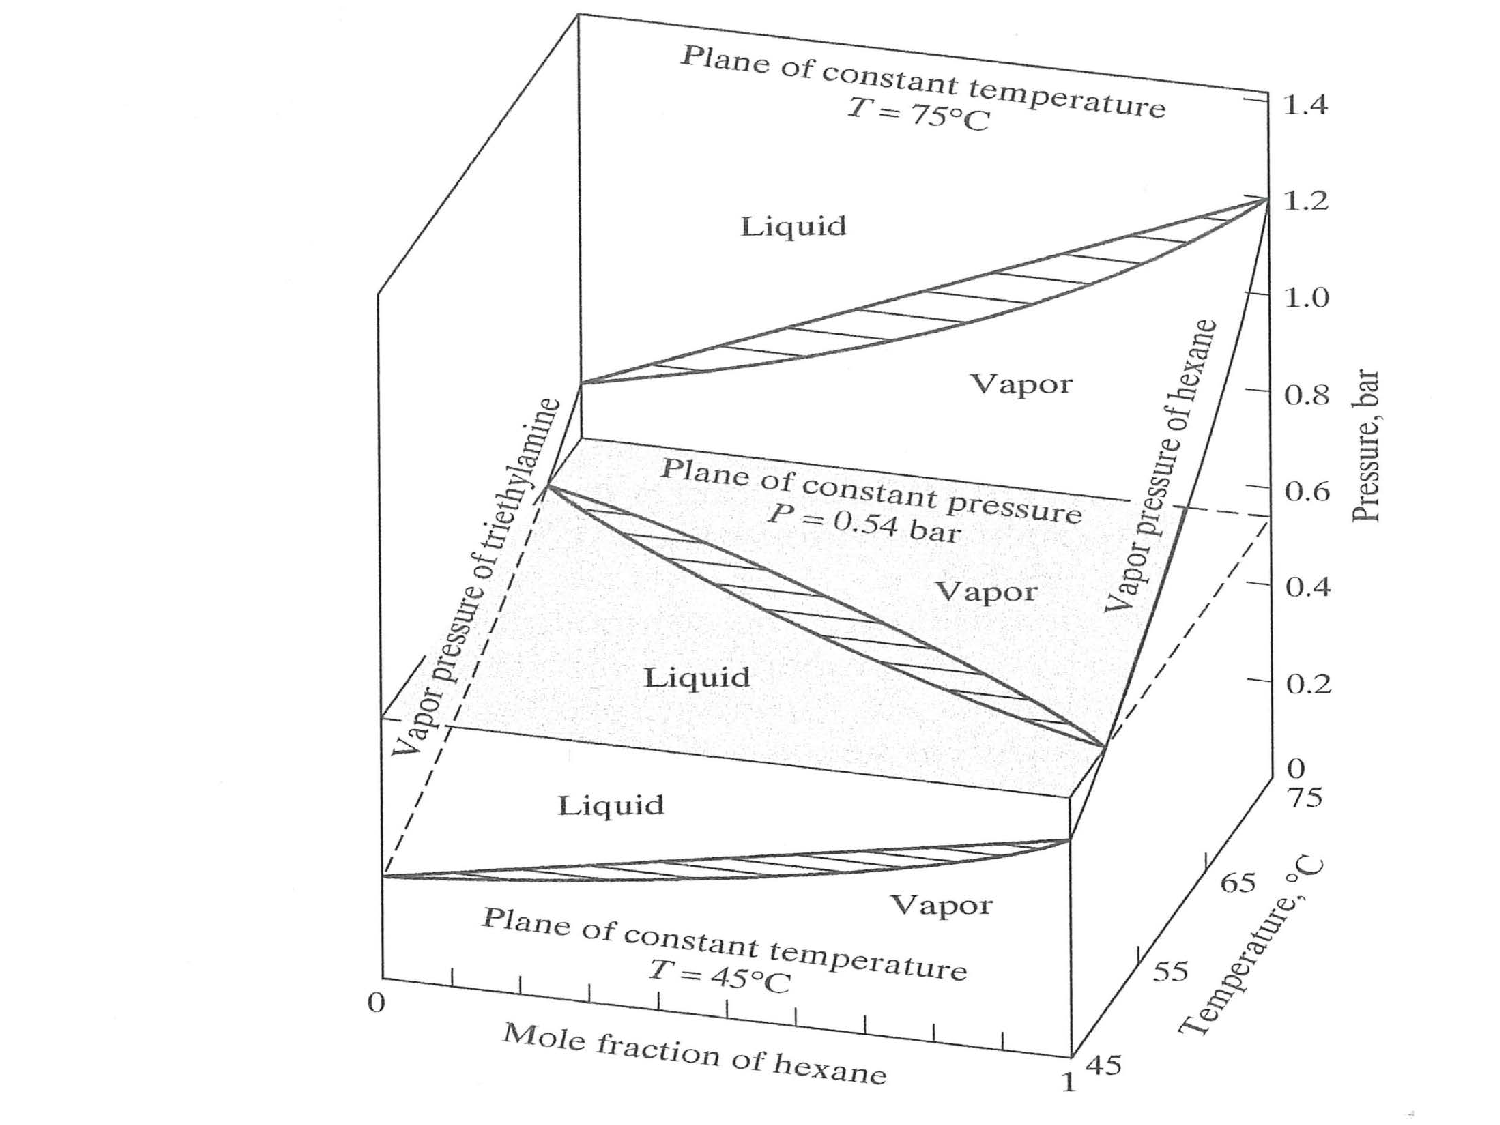
\includegraphics[width=.9\columnwidth,clip]{./../Pics/PTxy_diagram}
           \vspace{-.1cm}\caption{$P-T-xy$ diagram for hexane and triethylamine \citep[extracted from][]{Sandler_Book}.}\label{Chapter:VLE:Fig:Fig01}
         \end{center}
       \end{figure}

%%% SUBSECTION
\subsection{Qualitative Analysis: Phase Diagrams}\label{Chapter:VLE:Section:PhaseDiagrams}
In Section~\ref{Chapter:VolumetricPropertiesPureSubstances:Section:PVTBehaviour}, the {\it Gibbs phase rule} was introduced to help determining the number of degrees of freedom of any system,\index{Phase rule}\index{Phase rule !Degrees of freedom}
    \begin{displaymath}
        \Psi = 2 + \mathcal{C} - \mathcal{P}.
    \end{displaymath}
For a binary system in equilibrium (\ie $\mathcal{C}=2$), the phase rule yields a degree of freedom of $\Psi=4-\mathcal{P}$. In VLE systems ($\mathcal{P}=2$), the number of independent intensive variables becomes 2, and it will need to be chosen between:
\begin{enumerate}[a)]
   \item temperature ($T$);
   \item pressure ($P$);
   \item molar fraction of the more volatile component\footnote{In this chapter, for a mixture of $\mathcal{C}$ chemical species, the most volatile component will be assigned as number 1. Also, we will follow here the notation used in most thermodynamic text-books in which the molar fraction of component $i$ in vapour and liquid phases are \blue{$y_{i}$} and \blue{$x_{i}$}, respectively.} in the vapour phase $\left(y_{1}\right)$, and;
   \item molar fraction of the more volatile component in the liquid phase $\left(x_{1}\right)$.
\end{enumerate}
As shown in Fig.~\ref{Chapter:VLE:Fig:Fig01}, a plot with these 4 variables for a mixture of hexane and triethylamine is not very practical. In this $P-T-xy$ diagram, to ensure a single phase system $\left(\mathcal{P}=1\right)$, temperature, pressure and {\bf one} molar fraction need to be fixed. For a two-phase system $\left(\mathcal{P}=2\right)$, two variables need to be fixed and the system is expressed as a surface -- \eg the plane of constant pressure of $0.54$ bar. %Although insightful, this plot is not very convenient to assess compositions and phase behaviour, and is limited to a binary systems.
%%%% FIGURE
      \begin{figure}[h] 
         \begin{center}
             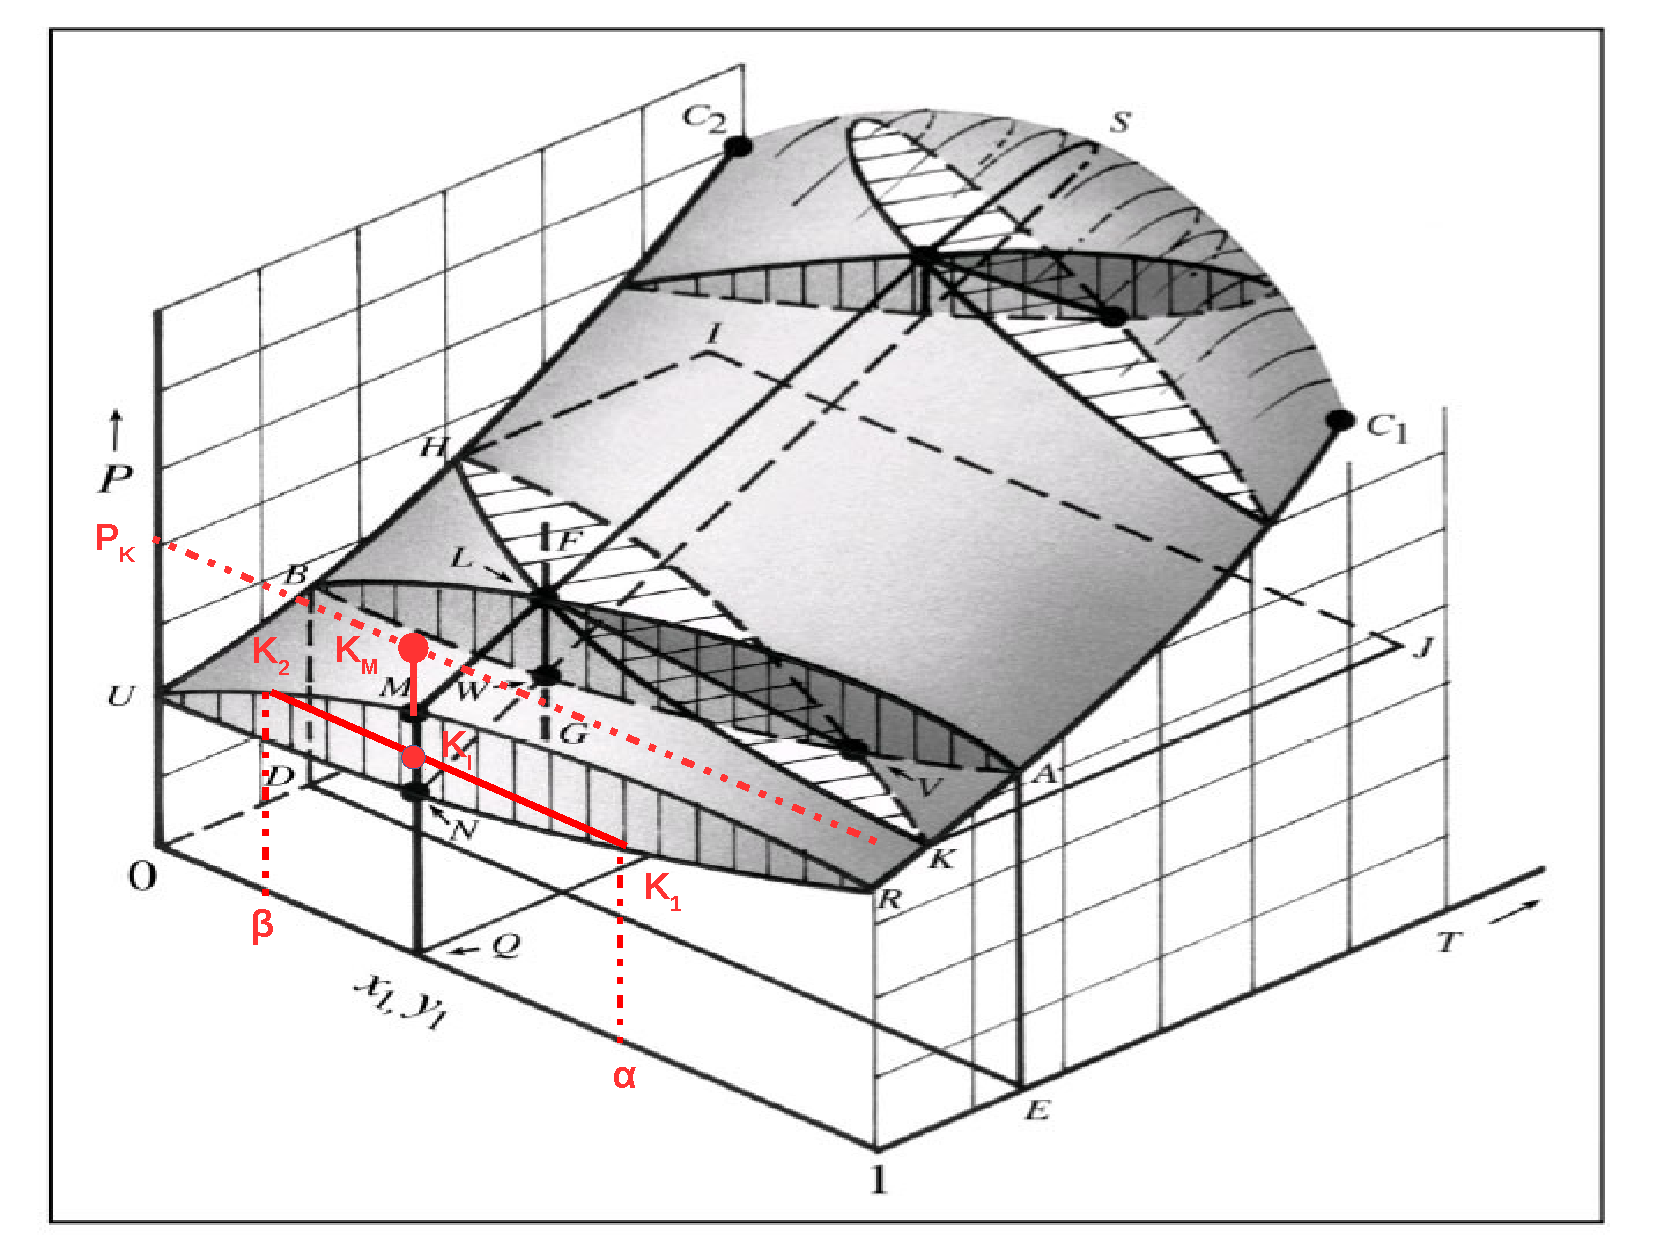
\includegraphics[width=.75\columnwidth,clip]{./Figs/PTxy_Digram} 
             \vspace{-.1cm}\caption{$P-T-xy$ diagram for binary mixtures \citep[extracted from][]{SmithVanNess_Book}.}\label{Chapter:VLE:Fig:Fig02}
         \end{center}
       \end{figure}

In a generic $P-T-xy$ diagram (Fig.~\ref{Chapter:VLE:Fig:Fig02}), vertical planes parallel to the \blue{0-1-R-M-U-0} plane (\eg plane \blue{E-A-B-D-E}) indicates $P-xy$ diagrams at constant temperature, whereas horizontal planes parallel to the \blue{K-J-I-H-K} plane indicates $T-xy$ diagrams at constant pressure. The liquid (\ie subcooled) region lies \underline{above} the upper-surface of the solid (grey) projection (solid body bounded by \blue{U-R-C$_{1}$-C$_{2}$-U}), and (superheated) vapour region lies \underline{below} the under-surface. The interior of the solid projection between the two surfaces is the region of coexistence of both liquid and vapour phases. 
%%% FIGURE
      \begin{figure}[h]
        \vbox{\hbox{\hspace{0.cm}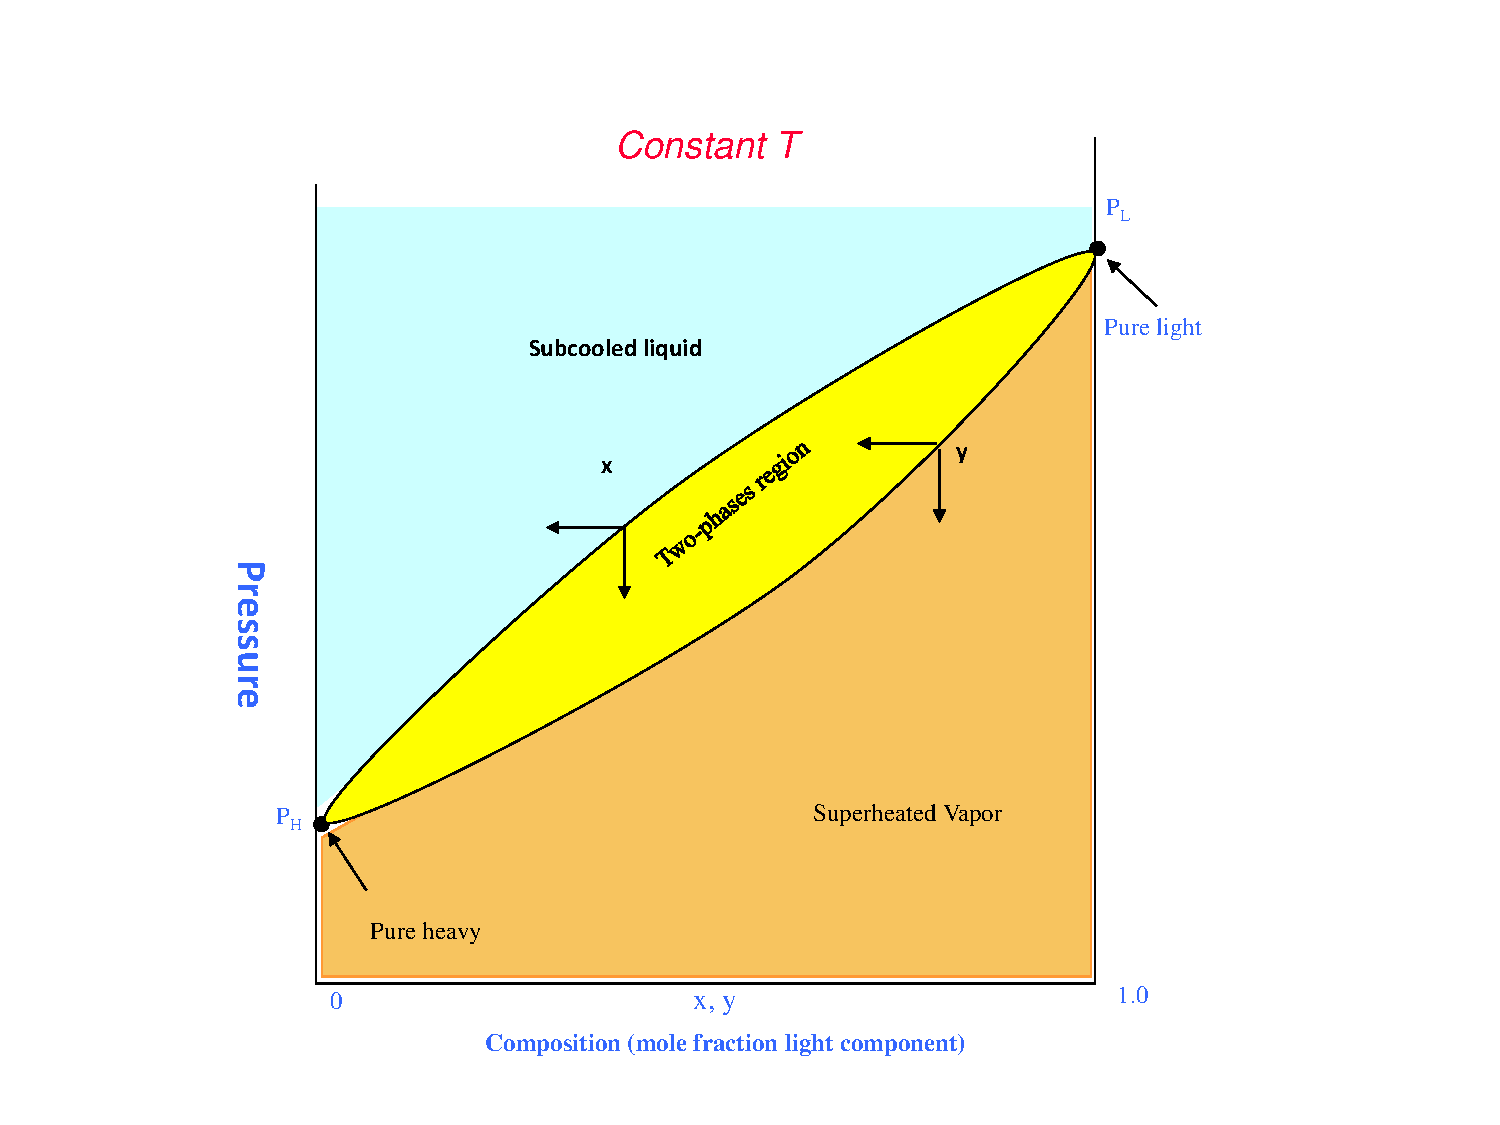
\includegraphics[width=.5\linewidth,clip]{./../Pics/VLE_Pxy_Diagram1}
            \hspace{-2.cm}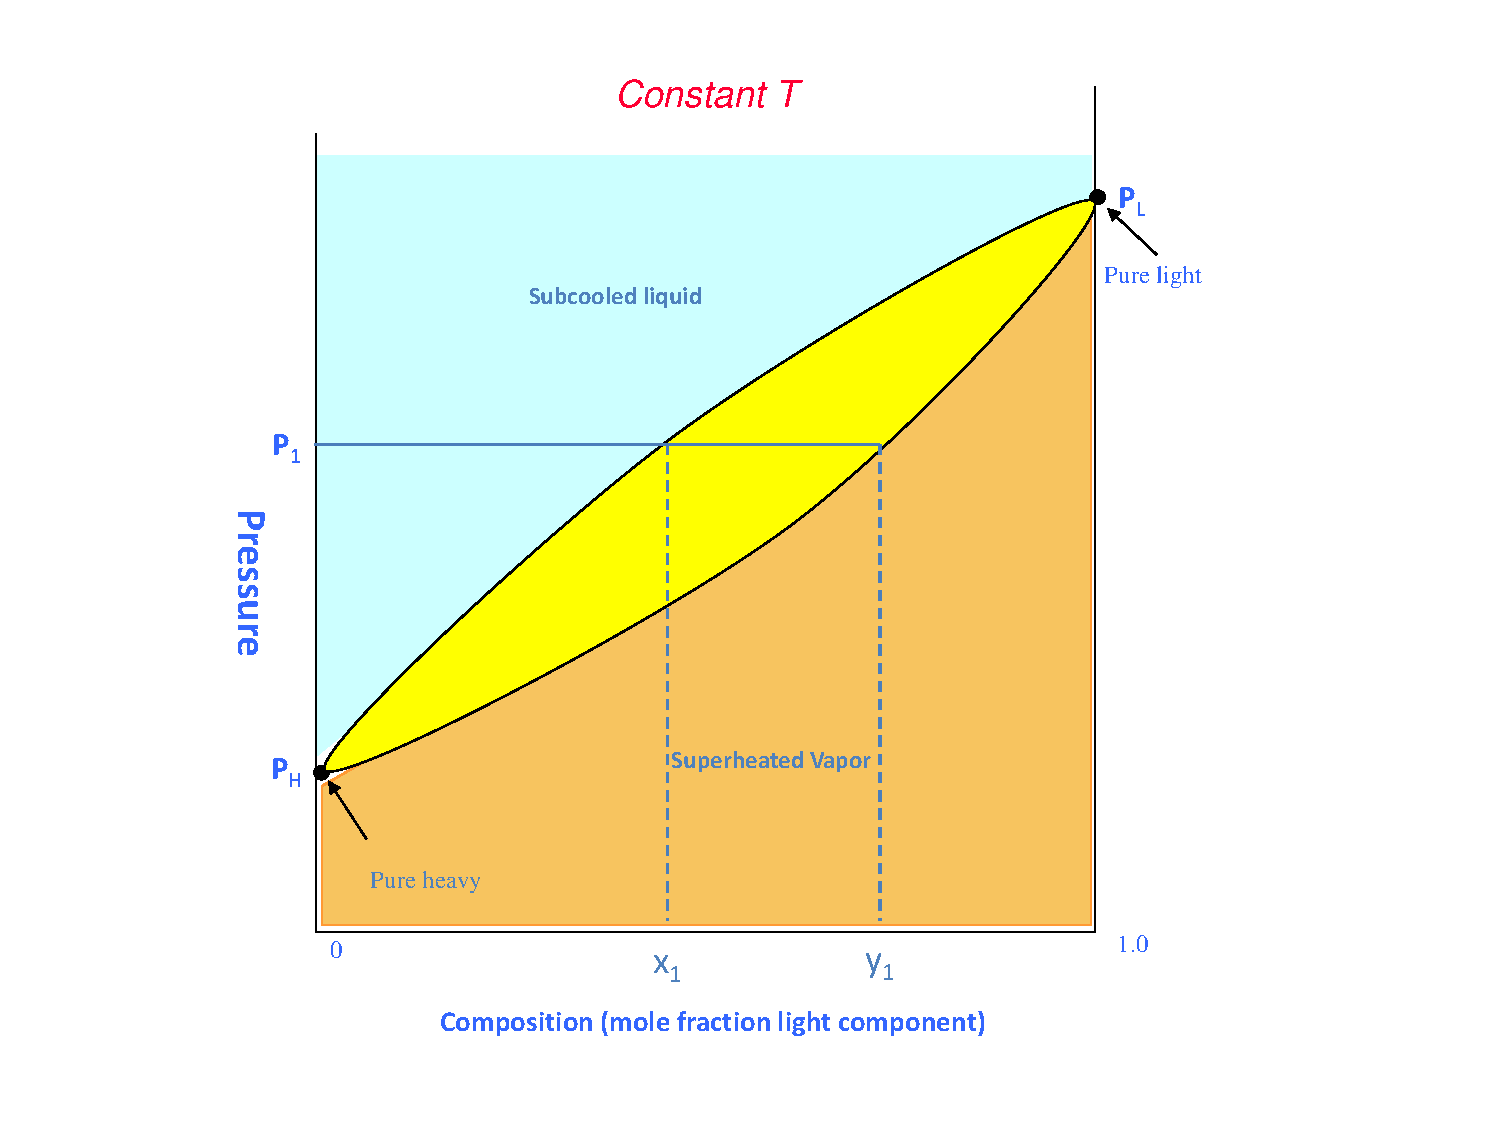
\includegraphics[width=.5\linewidth,clip]{./../Pics/VLE_Pxy_Diagram2}}
          \vspace{-0.5cm}
          \hbox{\hspace{3.5cm}(a)\hspace{6cm}(b)}
          \vspace{-0.cm}
          \hbox{\hspace{3.cm}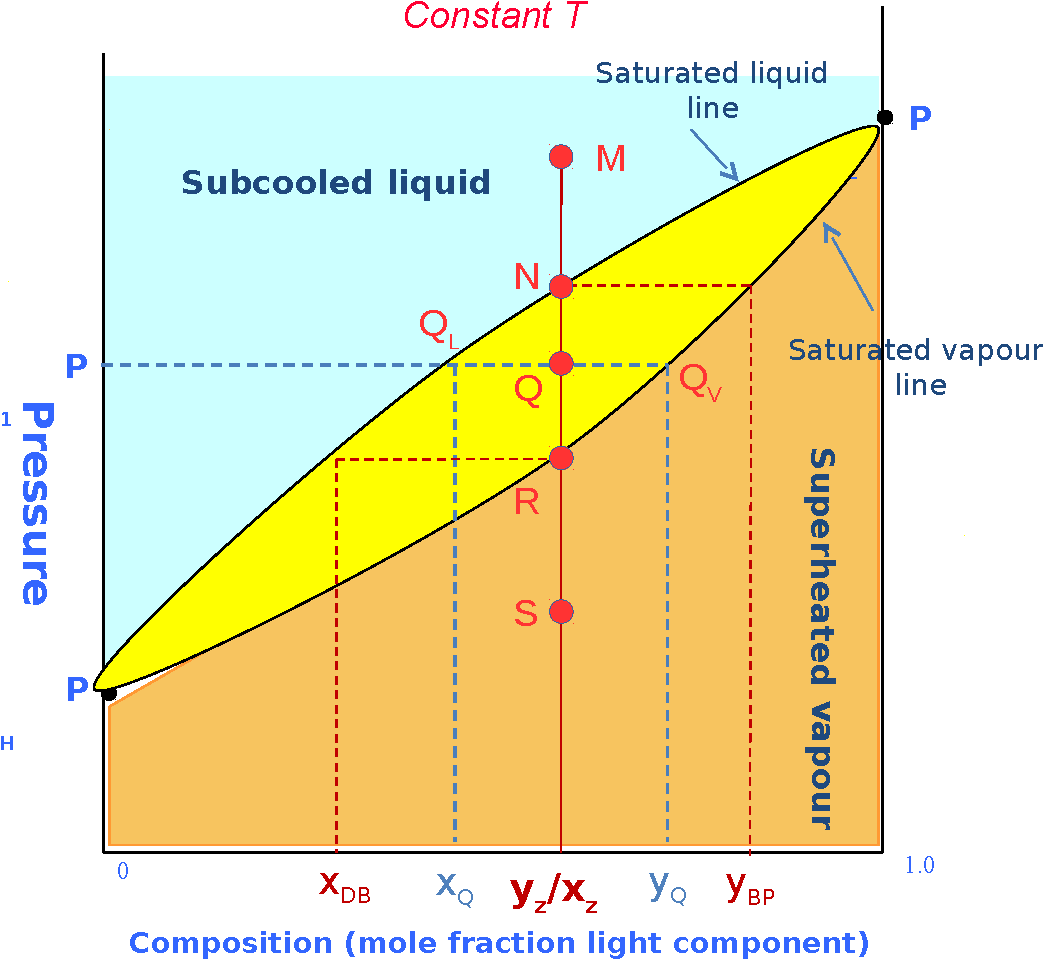
\includegraphics[width=.5\linewidth,clip]{./../Pics/VLE_Pxy_Diagram3b}}
          \vspace{-.1cm}
          \hbox{\hspace{6.8cm}(c)}}
        \vspace{-.1cm}\caption{VLE for binary mixtures: $P-xy$ diagrams at constant temperature.}\label{Chapter:VLE:Fig:Fig03}
      \end{figure}

The $x_{1},y_{1}$ axis is limited to \blue{zero} and \blue{one}, thus at $x_{1}$ (or $y_{1}$) equal to zero, $x_{2}$ (or $y_{2}$) is equal to unity, \ie there is just pure component \blue{2} in solution. Similarly at $x_{1}$ (or $y_{1}$) equal to one, $x_{2}$ (or $y_{2}$) is equal to zero, \ie there is just pure component \blue{1} in solution. The diagram also depicts points \blue{$C_{1}$} and \blue{$C_{2}$} along the vertical planes of $x_{1},y_{1}=0$ and $x_{1},y_{1}=1$, respectively. These two points are the coordinates of the critical conditions $\left(P_{c,1}, P_{c,2}, T_{c,1} \text{ and } T_{c,2}\right)$ of both \underline{pure components}. Critical coordinates for mixtures at various compositions of \blue{1} and \blue{2} lie along a line on the rounded edge of the surface between \blue{$C_{1}$} and \blue{$C_{2}$}.

For each constant temperature plane (vertical), the upper line of the solid (grey) projection is the \blue{saturated liquid line} whilst the lower line is the \blue{saturated vapour line} (the reader should remember that these lines are also present for pure substances in the $Ts$ and $Ph$ diagrams, Fig.~\ref{Chapter:ThermodynamicPropertiesPureFluids:Fig:Fig02}).

Compositions of each phase can be obtained from a parallel line linking $x_{1}$ and $y_{1}$. For example, in the `lens' \blue{U-M-R-N-U} contained in the plane \blue{0-U-M-R-1-Q-0}, the vapour phase (with composition \red{$y_{1}=\alpha$}  at $\left.\blue{K_{1}}\right)$ is in equilibrium with the liquid phase $\left(\text{with composition }\red{x_{1}=\beta}\text{ at } \blue{K_{2}}\right)$. This parallel line, \blue{$K_{1}-K_{2}$}, is called \underline{tie-line} (Fig.~\ref{Chapter:VLE:Fig:Fig03}b). The intersection of the tie-line with the saturated liquid line is referred as \blue{bubble pressure}, and the intersection with the saturated vapour line is called \blue{dew pressure} (at constant temperature).
%%% FIGURE
     \begin{figure}[h]
        \vbox{\hbox{\hspace{3.cm}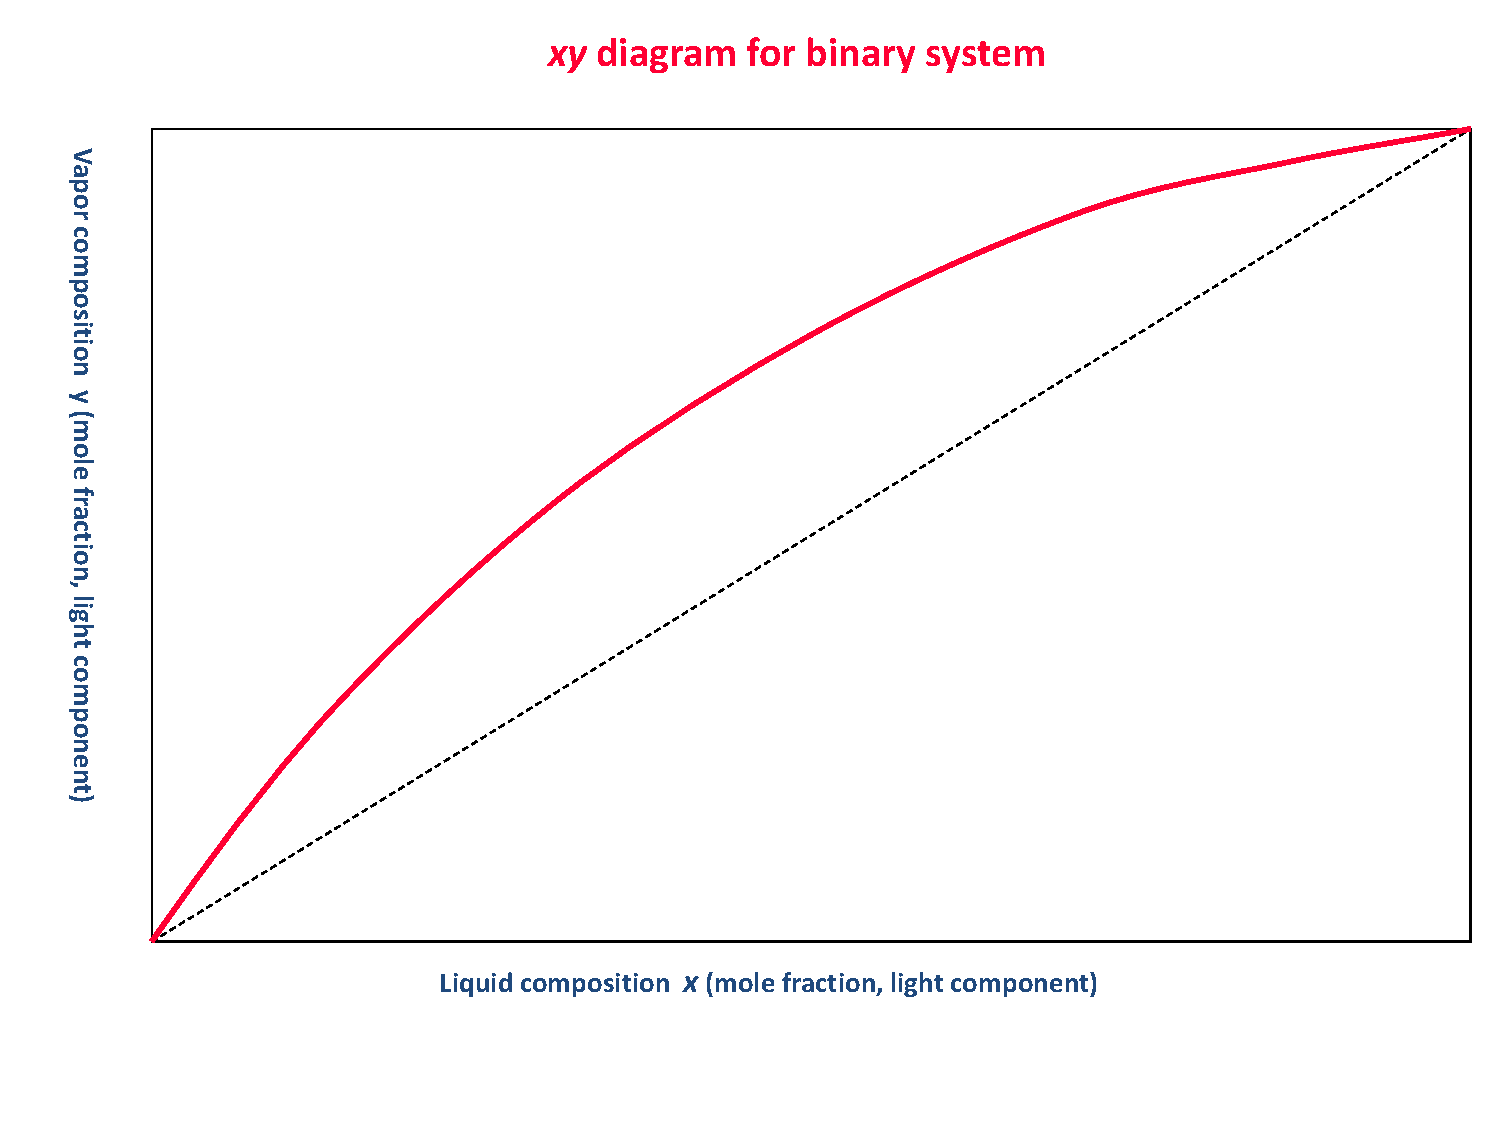
\includegraphics[width=.6\linewidth,clip]{./../Pics/VLE_xy_DiagramIdeal}}
          \vspace{-.5cm}
          \hbox{\hspace{8.cm}(a)}
          \hbox{\hspace{-1.cm}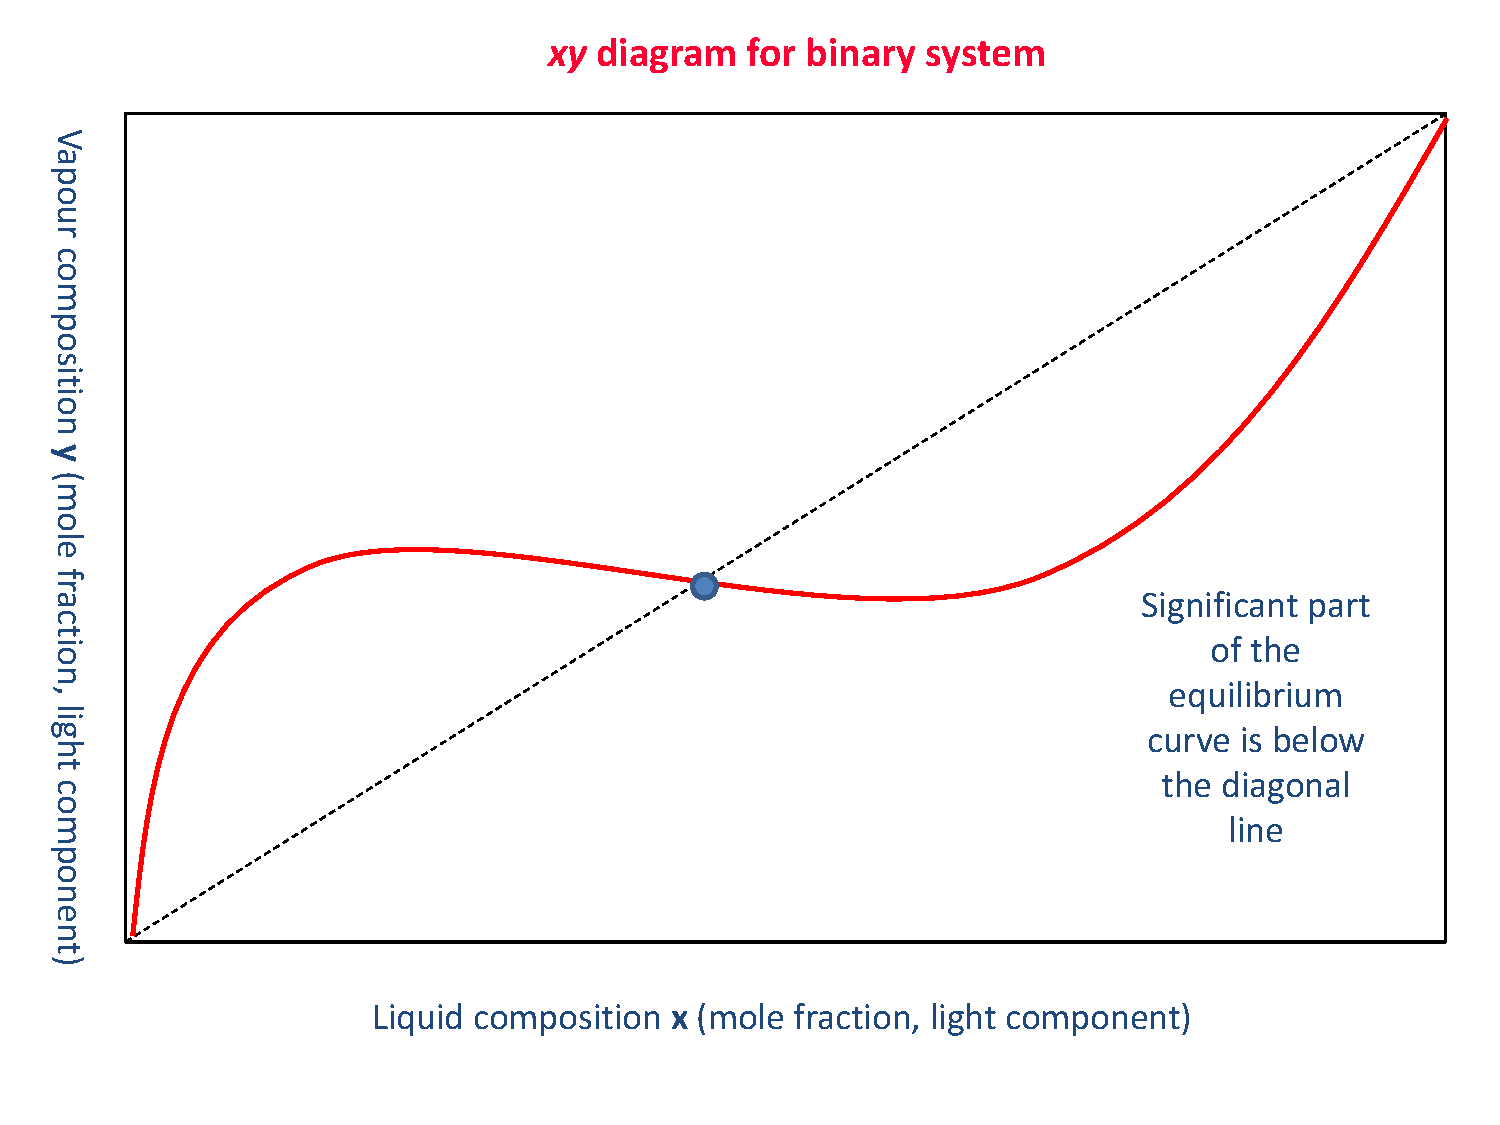
\includegraphics[width=.5\linewidth,clip]{./../Pics/VLE_xy_DiagramNonIdeal1}
            \hspace{-0.cm}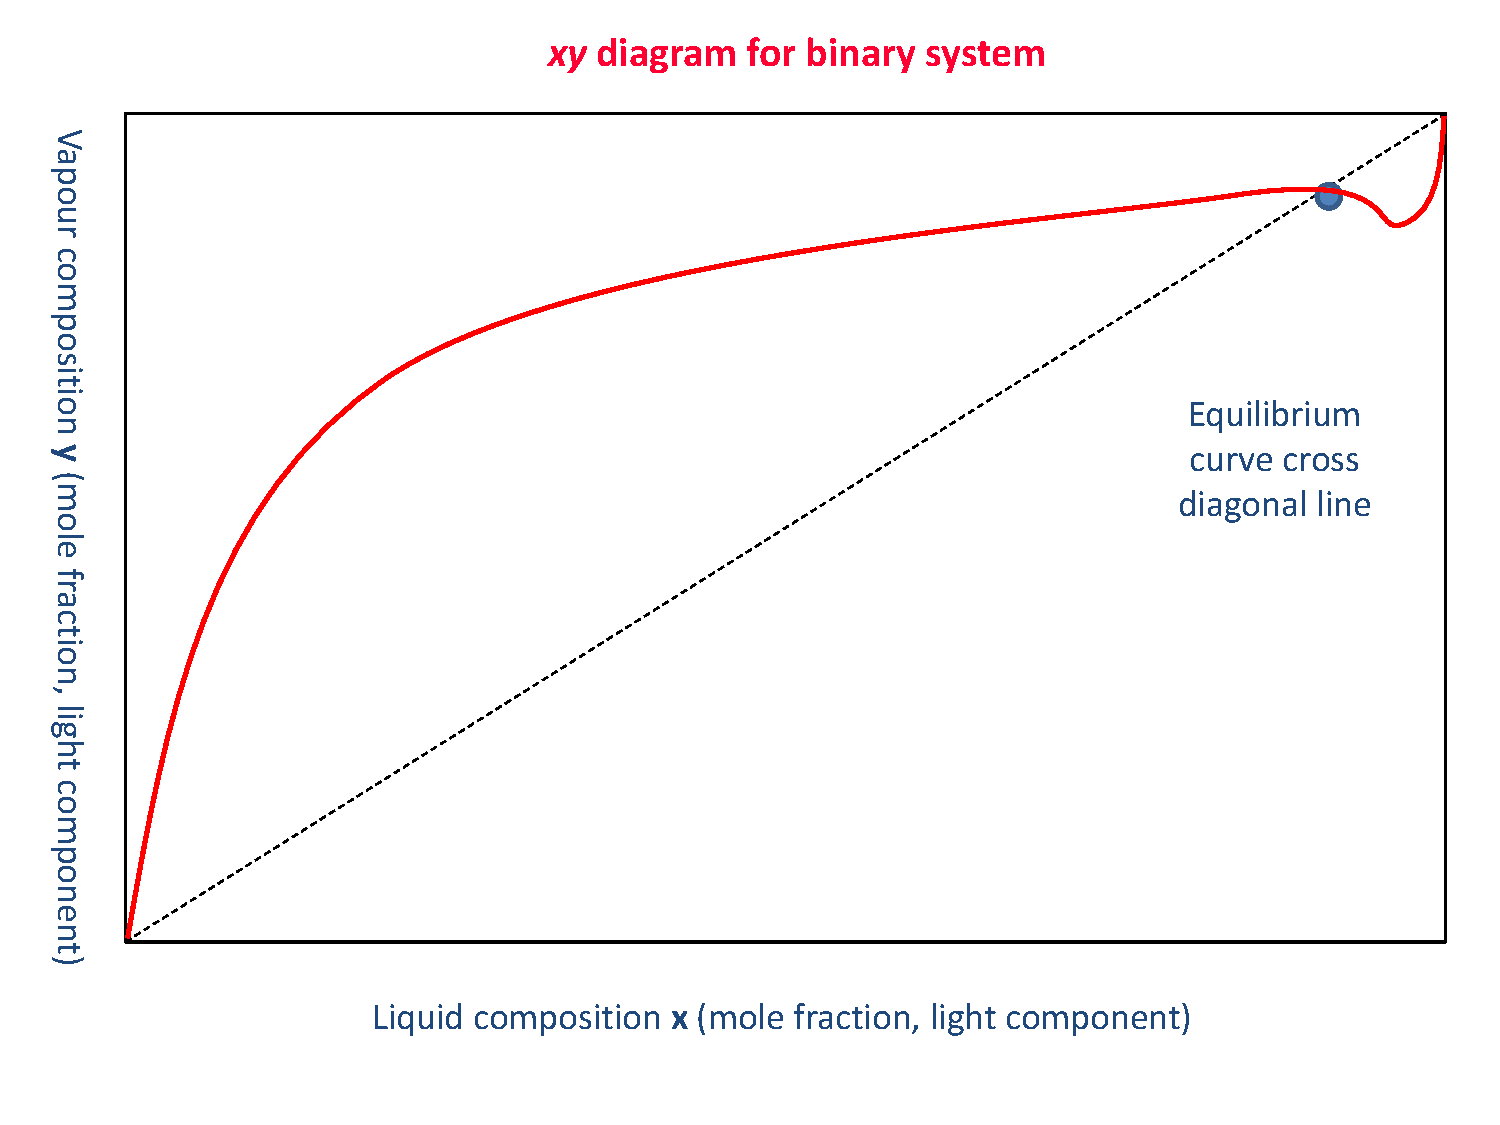
\includegraphics[width=.5\linewidth,clip]{./../Pics/VLE_xy_DiagramNonIdeal2}}
          \vspace{-.5cm}
          \hbox{\hspace{3.5cm}(b)\hspace{7.5cm}(c)}}
          \vspace{-.1cm}\caption{VLE for binary mixtures: $xy$ diagrams at constant pressure of (a) ideal and (b-c) non-ideal solutions.}\label{Chapter:VLE:Fig:Fig04}
      \end{figure}

$P-T-xy$ diagram, although insightful, is not very practical. Projections of $P-xy$ plane at constant temperature are shown in Fig.~\ref{Chapter:VLE:Fig:Fig03}. Now, let's assume that the fluid of Fig.~\ref{Chapter:VLE:Fig:Fig03}(c) is at liquid phase at coordinate \blue{$M$} with composition \blue{$\left(x_{1}=x_{z};y_{1}=0\right)$}. As pressure is reduced along the \blue{$M-S$} line, the first bubble of vapour appears at \blue{$N$}; composition at this coordinate is \blue{$\left(x_{1}=x_{z};y_{1}=y_{BP}\right)$}, and this is called \blue{\it bubble point}. Further reduction of pressure to coordinate \blue{$Q$} (still at constant temperature), the fluid becomes partially vaporised and the composition at this coordinate is given by the {\it tie-line} \blue{$Q_{L}-Q_{V}$} -- \blue{$\left(x_{1}=x_{Q};,y_{1}=y_{Q}\right)$}. \index{Bubble point}

As the pressure is continuously reduced along line \blue{$Q-R$}, more liquid is vaporised until \blue{$R$}, when the last droplet of liquid (dew) is vaporised. This coordinate is called \blue{\it dew point}. The composition at $N$ is \blue{$\left(x_{1}=x_{DB};y_{1}=y_{z}\right)$}. Continued reduction of pressure towards \blue{$S$} leads to (pure) vapour region with composition \blue{$\left(x_{1}=0,y_{1}=y_{z}\right)$}.\index{Dew point}

     Another common phase diagram is the $x-y$, Fig.~\ref{Chapter:VLE:Fig:Fig04}(a), in which either pressure or temperature is kept constant. In this diagram, at constant pressure, there are two curves, the upper curve represents the composition at equilibrium with varying temperature. The straight line represents the equimolar composition, \ie $x_{1}=y_{1}$. However, in several solutions of industrial interest, molecular attractive forces from the heavier component (2) keep molecules of the more volatile component in the liquid solution, constraining its evaporation. This leads into an equilibrium pressure smaller than the expected at the same liquid composition. Such deviation from ideality is called \blue{\it azeotropy}. In practical terms, any component from solutions can often be separated through distillation processes, however azeotropes may lead to vapour-liquid-liquid equilibrium (VLLE) and other separations strategies may need to be used.\index{Azeotropy}
     
%%% SUBSECTION
\subsection{VLE Models: Raoult's Law}\label{Chapter:VLE:Section:RaoultsLaw}
  \begin{subequations}
      The diagrams of binary (as well as multi-component) mixtures shown in the previous section are obtained from experiments and introduce a qualitative analysis of the PVT behaviour of solutions. However, classic thermodynamics provides a mathematical framework for systematic correlation, extension, generalisation and interpretation of data.\index{Raoult's law|see {Solutions}}\index{Solutions!Raoult's law}
      \begin{shaded}
        For ideal vapour-liquid systems, the \blue{Raoult's law} provides a relation between the compositions of the vapour and liquid phases,
           \begin{equation}
             P_{i} = y_{i}P = x_{i}P_{i}^{\text{sat}},\;\;\;\forall i\in\left\{1,2,\cdots,\mathcal{C}\right\},\label{Chapter:VLE:Eqn:RaoultLaw} 
           \end{equation}
      \end{shaded}
      where $P_{i}$ is known as  partial pressure (Eqn.~\ref{Chapter:Intro_Property_of_Gases:Eqn:PartialPressure_1}) and $P_{i}^{\text{sat}}$ is the saturated pressure (or saturated vapour pressure) of pure species $i$ and was defined in Section~\ref{Chapter:ThermodynamicPropertiesPureFluids:Section:ClapeyronRelations}. This rather simple relation can only be applied to ideal solutions (for both phases). For a gas mixture to be considered ideal the pressure need to be equal or smaller than atmospheric. There are several relations for ideal gas mixtures, \eg\index{Pressure!Partial}
       \begin{enumerate}[a)]
               \item Dalton's Law (Section~\ref{Chapter:Intro_Property_of_Gases:Section:MixtureGases}):\index{Gases!Dalton's law}
                  \begin{equation}
                      P = \summation[P_{i}]{i=1}{\mathcal{C}} = \summation[y_{i}P]{i=1}{\mathcal{C}}\label{Chapter:VLE:Eqn:PartialMolarProperties:DaltonLaw}
                  \end{equation}
           \item Amagat's Law:\index{Gases!Amagat's law}\index{Amagat's law|see {Gases}}
              \begin{equation}
                  V^{\text{t}} = \summation[V_{i}]{i=1}{\mathcal{C}} = \summation[y_{i}V^{\text{t}}]{i=1}{\mathcal{C}}\label{Chapter:VLE:Eqn:PartialMolarProperties:AmagatLaw}
              \end{equation}
           \item Kay's rule for pseudo-critical temperature and pressure:\index{Gases!Kay's law}\index{Kay's law|see {Gases}}
              \begin{equation}
                  T_{c}^{\text{t}} = \summation[y_{i}T_{c,i}]{i=1}{\mathcal{C}},\;\;\text{ and }\;\;P_{c}^{\text{t}} = \summation[y_{i}P_{c,i}]{i=1}{\mathcal{C}}\label{Chapter:VLE:Eqn:PartialMolarProperties:KayLaw}
              \end{equation}
       \end{enumerate}
       Liquid solutions are considered ideals if the molecular interaction between the similar species is identical to that between dissimilar species. Thermodynamics of liquid solutions are the main focus of Chapter~\ref{Chapter:SolutionThermodynamics}.
       
  \end{subequations}

  \medskip
   % Example
   \begin{MyExample}{\begin{center}{\bf Example}\end{center}}
     \begin{example}\label{Chapter:VLE:Example1}
       Assuming a mixture of n-pentane $\left(nC_{5}\right)$ and n-heptane $\left(nC_{7}\right)$ is ideal, draw vapour-liquid $x_{5}\times y_{5}$ and $P-x_{5}y_{5}$ equilibrium diagrams for this mixtures at constant temperature of 50$^{\circ}$C. Given $P^{\text{sat}}$ relation,
       \begin{displaymath}
         \ln{P_{i}^{\text{sat}}} = A_{i} - \frc{B_{i}}{RT}
       \end{displaymath}
       with $A_{nC_{5}}=10.422$, $A_{nC_{7}}=11.431$, $B_{nC_{5}}=26799 \text{ J.mol}^{-1}$ and $B_{nC_{7}}=35200 \text{ J.mol}^{-1}$. Also [$P$] = bar and [$T$] = K.
     \end{example}

% SOLUTION
     \noindent{\bf Solution:}
        At $T=$50$^{\circ}$C = 323.15 K, vapour saturated pressures for $nC_{5}$ and $nC_{7}$ (for short notation, let's use 5 and 7 as $nC_{5}$ and $nC_{7}$, respectively) are
           \begin{displaymath}
              P_{5}^{\text{sat}} = 1.5639\text{ bar}\;\;\text{ and }\;\;P_{7}^{\text{sat}} = 0.1881\text{ bar}.
           \end{displaymath}
           In order to calculate the equilibrium pressure at each liquid $nC_{5}$ composition, $x_{5}$,
           \begin{eqnarray}
               && P_{i} = x_{i}P_{i}^{\text{sat}} \;\;\Longleftrightarrow \;\; P = \summation[P_{i}]{i=1}{\mathcal{C}} = \summation[x_{i}P_{i}^{\text{sat}}]{i=1}{\mathcal{C}} \nonumber \\
               && P = x_{5}P_{5}^{\text{sat}} + x_{7}P_{7}^{\text{sat}} = x_{5}P_{5}^{\text{sat}} + \left(1-x_{5}\right)P_{7}^{\text{sat}} \nonumber 
           \end{eqnarray}
           And for vapour composition (Raoult's law),
           \begin{displaymath}
               y_{i} P = x_{i}P_{i}^{\text{sat}}  \;\;\Longleftrightarrow \;\; y_{5} = \frc{x_{5}P_{5}^{\text{sat}}}{P},
           \end{displaymath}
           replacing pressure, $P$, from the previous equation
           \begin{displaymath}
               y_{5} = \frc{x_{5}P_{5}^{\text{sat}}}{x_{5}P_{5}^{\text{sat}} + \left(1-x_{5}\right)P_{7}^{\text{sat}}}.
           \end{displaymath}
           The $x_{5} \times y_{5}$ diagram may be plot by giving values to $0.0\leq x_{5} \leq 1.0$ and calculating $x_{5}$ through the equation above.

           The $P-x_{5}y_{5}$ diagram may be plot using the relations,
           \begin{displaymath}
               y_{5} = \frc{x_{5}P_{5}^{\text{sat}}}{P}\;\;\;\text{ and }\;\;\; P = x_{5}P_{5}^{\text{sat}} + \left(1-x_{5}\right)P_{7}^{\text{sat}} \;\Longrightarrow\; x_{5} = \frc{P-P_{7}^{\text{sat}}}{P_{5}^{\text{sat}}-P_{7}^{\text{sat}}}.
           \end{displaymath}
           Thus, given values for $P_{7}^{\text{sat}}\leq P \leq P_{5}^{\text{sat}}$ $\Rightarrow$ Calculate $x_{5}$  $\Rightarrow$ Calculate $y_{5}$.
           \bigskip
           
           \hbox{
             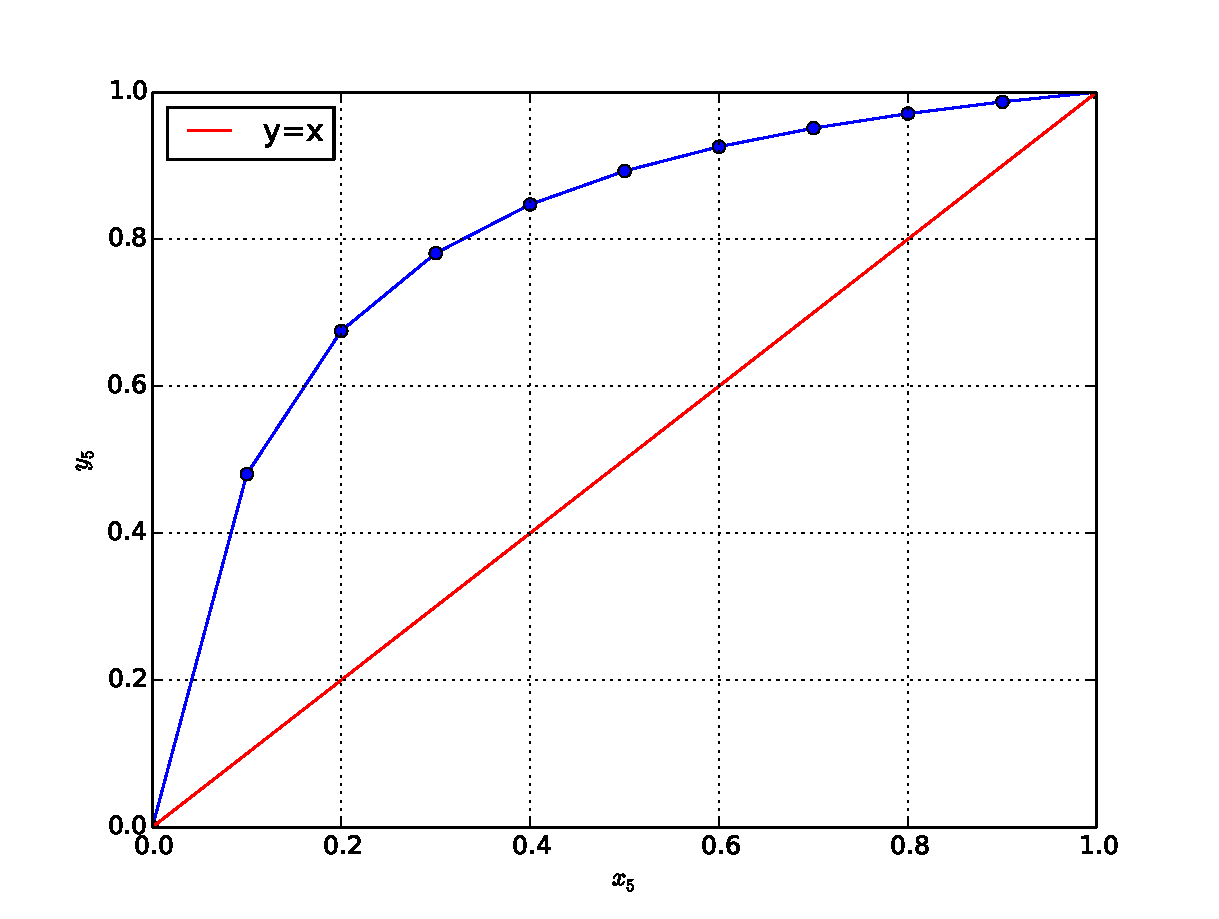
\includegraphics[width=.5\linewidth,clip]{./Figs/Mod4Ex1}
             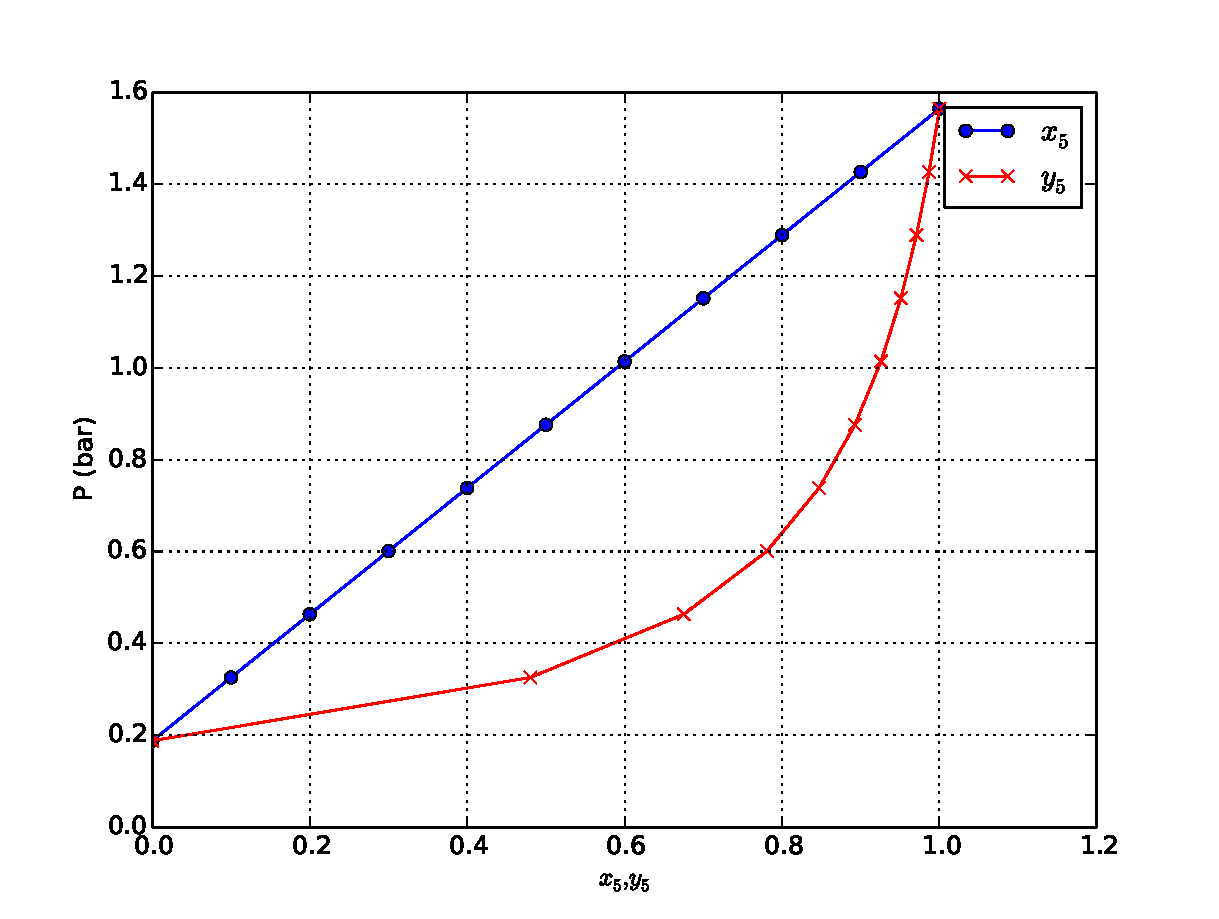
\includegraphics[width=.5\linewidth,clip]{./Figs/Mod4Ex1b}}
           
   \end{MyExample} 

  \medskip
   % Example
   \begin{MyExample}{\begin{center}{\bf Example}\end{center}}
     \begin{example}\label{Chapter:VLE:Example2}
       Assuming a mixture of n-pentane $\left(nC_{5}\right)$ and n-heptane $\left(nC_{7}\right)$ is ideal, draw vapour-liquid $x_{5}\times y_{5}$ and $T-x_{5}y_{5}$ equilibrium diagrams for this mixtures at constant pressure of 1.013 bar. Given $P^{\text{sat}}$ relation,
    \begin{displaymath}
      \ln{P_{i}^{\text{sat}}} = A_{i} - \frc{B_{i}}{RT}
    \end{displaymath}
    with $A_{nC_{5}}=10.422$, $A_{nC_{7}}=11.431$, $B_{nC_{5}}=26799 \text{ J.mol}^{-1}$ and $B_{nC_{7}}=35200 \text{ J.mol}^{-1}$. Also [$P$] = bar and [$T$] = K.
     \end{example}

% SOLUTION
     \noindent{\bf Solution:}
     In this problem, equilibrium temperature and compositions are not known, thus
          \begin{displaymath}
              P = x_{5}P_{5}^{\text{sat}} + x_{7}P_{7}^{\text{sat}} = x_{5}P_{5}^{\text{sat}} + \left(1 - x_{5}\right)P_{7}^{\text{sat}} = 1.013\text{ bar},
          \end{displaymath}
          where $P_{i}^{\text{sat}}$ is non-linear function of the temperature $T$, \ie
          \begin{displaymath}
              P = x_{5}\exp{\left(A_{5} - \frc{B_{5}}{RT}\right)} + \left(1 - x_{5}\right)\exp{\left(A_{7} - \frc{B_{7}}{RT}\right)}.
          \end{displaymath}
          This equation has 2 unknowns, $x_{5}$ and $T$, however we know that $0.0\leq x_{5} \leq 1.0$, thus we can give values on this range $\Rightarrow$ calculate $T$  $\Rightarrow$  obtain $y_{5}$.
          \begin{center}
              \begin{tabular}{ c c c | c c c}
                  $\mathbf{x_{5}}$ & $\mathbf{T}${\bf(K)}  & $\mathbf{y_{5}}$ & $\mathbf{x_{5}}$ & $\mathbf{T}${\bf(K)}  & $\mathbf{y_{5}}$ \\
                    0.0000          & 370.80                & 0.0000         & 0.6000          & 323.13                & 0.9257          \\
                    0.1000          & 357.80                & 0.4050         & 0.7000          & 319.12                & 0.9528          \\
                    0.2000          & 347.73                & 0.6249         & 0.8000          & 315.60                & 0.9728          \\
                    0.3000          & 339.73                & 0.7535         & 0.9000          & 312.47                & 0.9881          \\
                    0.4000          & 333.21                & 0.8345         & 1.0000          & 309.67                & 1.0000          \\
                    0.5000          & 327.77                & 0.8881         &                 &                       &                 
              \end{tabular}
           \end{center}
           \medskip
             \hbox{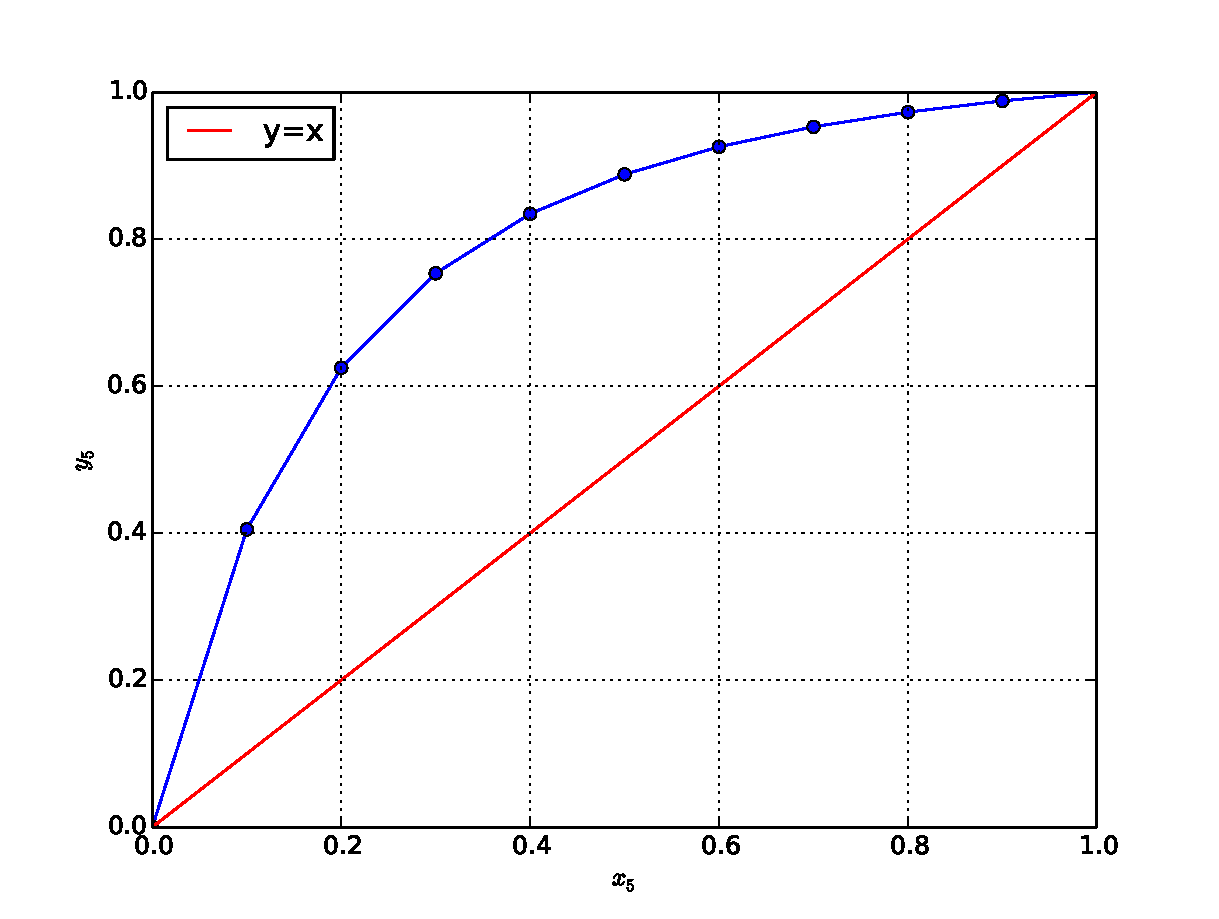
\includegraphics[width=.5\linewidth,clip]{./Figs/Mod4Ex2a}
                   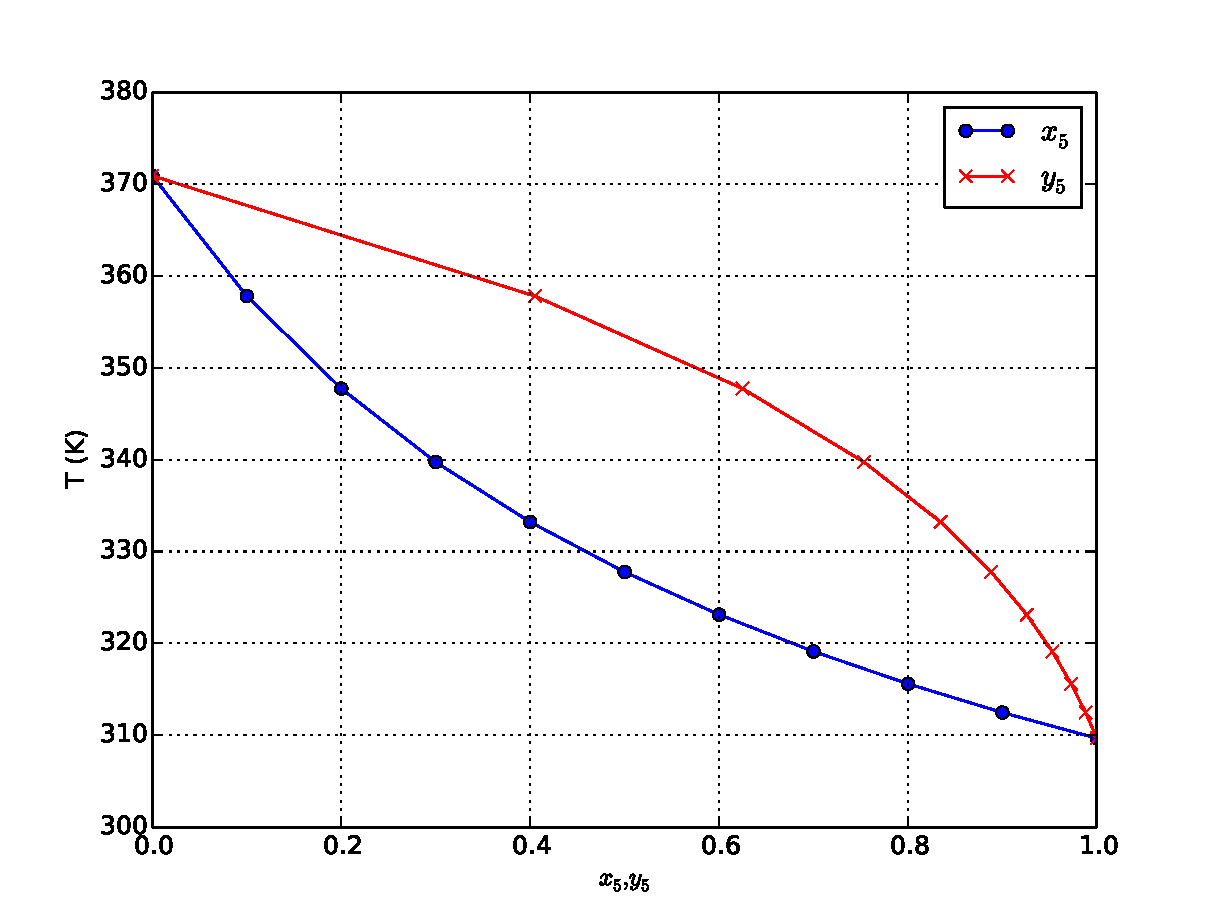
\includegraphics[width=.5\linewidth,clip]{./Figs/Mod4Ex2b}}
             
   \end{MyExample}

%%% SUBSECTION
\subsection{VLE Models: Henry's Law}\label{Chapter:VLE:Section:HenryLaw}\index{Henry's law|see {Solutions}}\index{Solutions!Henry's law}
A typical application of VLE is when gases are solubilised in liquid solutions, \eg O$_{2}$ in water, CO$_{2}$ in soft drinks, air in the blood stream etc. In these cases, gases have relatively low solubility (mole fraction varying between 10$^{-5}$ to 10$^{-2}$) in liquid solvents. In ideal solutions, both the more volatile (\ie solute) and the less volatile (\ie solvent) follow the Raoult’s law. However, for real solutions at low concentrations, although the vapour pressure $\left(P^{\text{sat}}\right)$ of the solute is proportional to its mole fraction, the constant of proportionality is not the vapour pressure of the pure substance. For such cases, a new relation is required that relates compositions in both phases and the pressure,
\begin{shaded}
  \begin{equation}
      P_{i} = y_{i}P = x_{i}\mathcal{H}_{i},\label{Chapter:VLE:Eqn:HenryLaw} 
  \end{equation}
\end{shaded}
\noindent where $\mathcal{H}$ is the Henry's constant obtained experimentally. Values of Henty's contant for several gases dissolved in water at 25$^{\circ}$C is shown in Table~\ref{Chapter:VLE:Table:HenryLawTable}
%%% TABLE
 \begin{table}
  \begin{center}
    \begin{tabular}{l r || l r }
      \hline
       {\bf Gas}    &  ${\bf \mathcal{H}\text{ (bar)}}$ & {\bf Gas}    &  ${\bf \mathcal{H}\text{ (bar)}}$ \\
      \hline
         Acetylene  &   1350                            & He           &  126600 \\
         Air        &   72950                           & H$_{2}$      &  71600  \\
         CO$_{2}$    & 1670                              & H$_{2}$S     & 550 \\
         CO         &  54600                            &  CH$_{4}$    &  41850 \\
         C$_{2}$H$_{6}$ & 30600                          &  N$_{2}$     & 87650  \\
         Ethylene  & 11550                              & O$_{2}$      & 44380 \\
      \hline
    \end{tabular}
    \caption{Henry's constant for gases dissolved in water at 25$^{\circ}$C.}\label{Chapter:VLE:Table:HenryLawTable}
  \end{center}
\end{table}

%%% SUBSECTION
\subsection{VLE Models: K-Value Correlations for Hydrocarbon Systems}\label{Chapter:VLE:Section:K_Values}\index{K-Value|see {Solutions}}\index{Solutions!K-Values}
As discussed in Section~\ref{Chapter:VolumetricPropertiesPureSubstances:Section:CubicEOS}, cubic equations of state are often used to describe the PVT behaviour of vapour and liquid phases of pure chemical species and mixtures. Although the use of cubic EOS is widely spread over the chemical industry, applicability to liquid phase is still limited. Several alternatives have been proposed and developed over the past 50 years, one of them, mostly used in petroleum and petrochemical industry for hydrocarbons, is called {\it K-value correlation}. $K$ is defined as
\begin{shaded}
   \begin{equation}
      K_{i} = \frc{P_{i}^{\text{sat}}}{P} = \frc{y_{i}}{x_{i}}.\label{Chapter:VLE:Eqn:KValue}
   \end{equation}
\end{shaded}
Values for $K_{i}$ are tabulated for a large number of hydrocarbons at several pressure and temperature conditions and can be found in any chemical engineering handbook as part of \blue{DePriester chart} (Fig.~\ref{Chapter:VLE:Fig:Fig05}).\index{DePriester chart|see {Solutions}}\index{Solutions!DePriester chart}
%%% FIGURE
  \begin{figure}[h]
     \begin{center}
         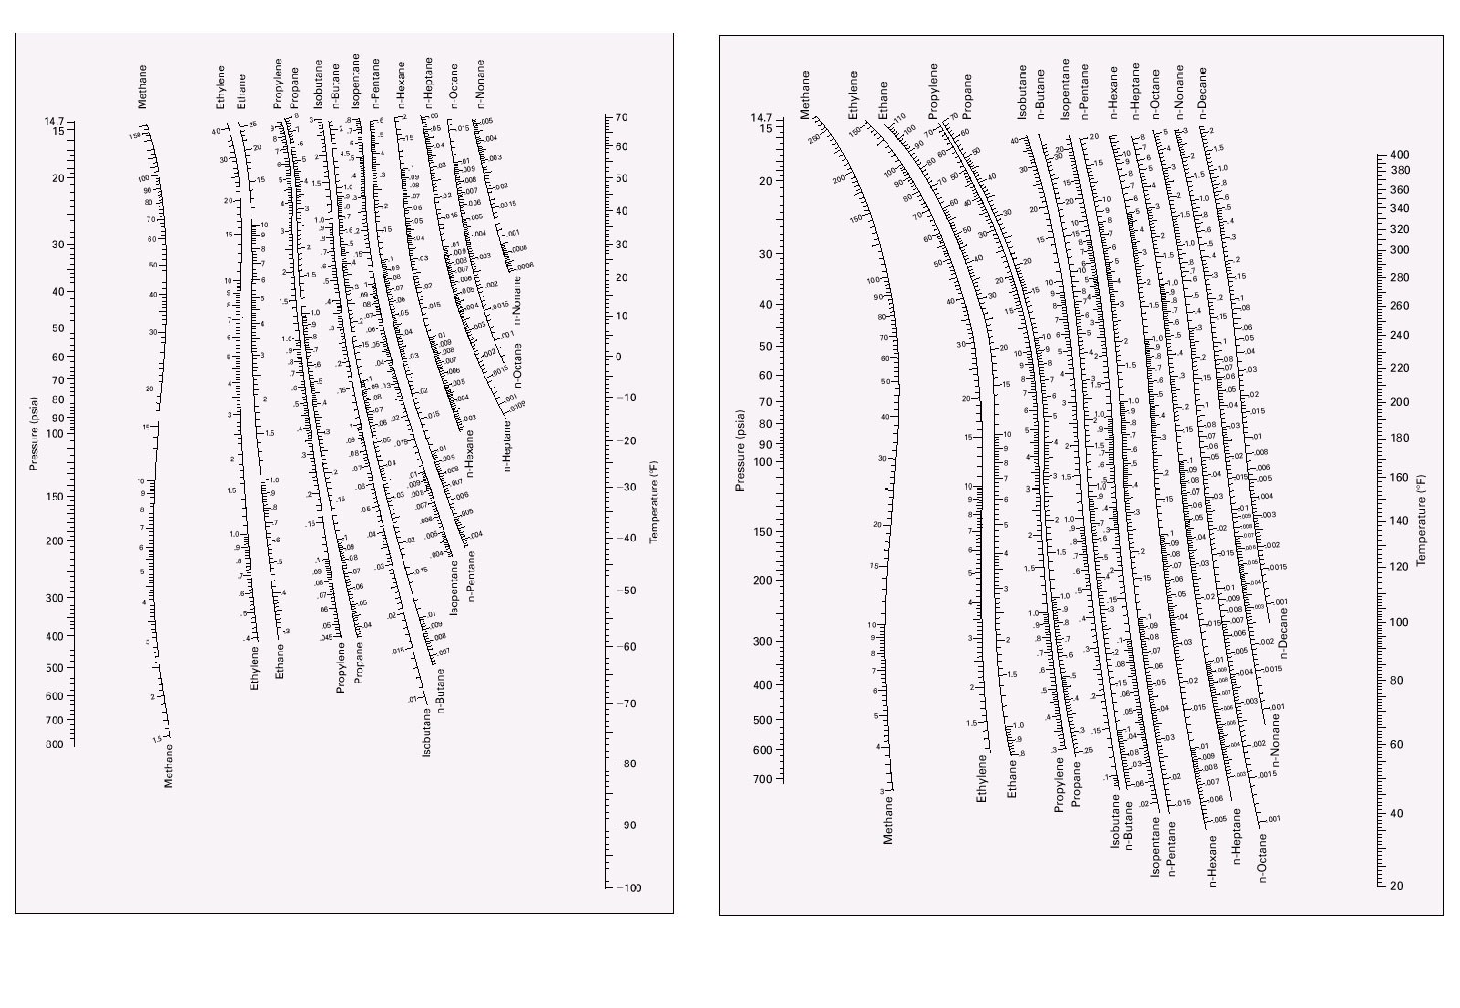
\includegraphics[width=1.\linewidth,clip]{./Figs/DePriesterCharts}
     \end{center}
     \caption{DePriester chart for several hydrocarbons \citep[extracted from][]{SmithVanNess_Book}.}\label{Chapter:VLE:Fig:Fig05}
  \end{figure}
  
%%% SECTION
  \section{Industrial Applications: Multi-Component VLE}\label{Chapter:VLE:Section:IndApplications}
  
%%% SUBSECTION
\subsection{Dew-point and Bubble-point Calculations using Raoult’s Law }\label{Chapter:VLE:Section:DewBubblePoint}\index{Bubble point}\index{Dew point}
Let's consider a vapour-liquid system containing $\mathcal{C}$ chemical species. From the phase rule the number of degrees of freedom is $\mathcal{C}$, that may be $T$, $P$, $x_{i}$ and/or $y_{i}$. Four types of problems are possible:
\begin{center}
   \begin{tabular}{|l c c|}
      \hline 
      $\mathbf{VLE}$ {\bf Problem} & {\bf Specified Variables} &  {\bf Computed Variables} \\  
      \hline
          {\bf Bubble Pressure}        &  $T$ and $x_{i}$           &   $P$ and $y_{i}$          \\
          {\bf Dew Pressure}           &  $T$ and $y_{i}$           &   $P$ and $x_{i}$          \\
          {\bf Bubble Temperature}     &  $P$ and $x_{i}$           &   $T$ and $y_{i}$          \\
          {\bf Dew Temperature}        &  $P$ and $y_{i}$           &   $T$ and $x_{i}$          \\     
      \hline
   \end{tabular}
\end{center}
Such problems are calculated using three relations:
\begin{displaymath}
    P_{i} = y_{i}P = x_{i}P_{i}^{\text{sat}}, \;\;\; \summation[x_{i}]{i=1}{\mathcal{C}} = 1, \;\;\text{ and }\;\; \summation[y_{i}]{i=1}{\mathcal{C}} = 1,
\end{displaymath}
bearing in mind that $P_{i}^{\text{sat}}$ is expressed as a function of $T$. Thus,
\begin{enumerate}[a)]
    \item Bubble pressure: Given $T$ and $x_{i}$ $\left(\text{with }i=1,\cdots,\mathcal{C}\right)$, find $P$ that solves,
        \begin{displaymath}
           \summation[y_{i}]{i=1}{\mathcal{C}} = 1 \;\;\Longrightarrow\;\; \summation[\frc{x_{i}P_{i}^{\text{sat}}}{P}]{i=1}{\mathcal{C}} = 1,
        \end{displaymath}
        and then calculate $y_{i}= \frc{x_{i}P_{i}^{\text{sat}}}{P}$.
        
    \item Bubble temperature: Given $P$ and $x_{i}$ $\left(\text{with }i=1,\cdots,\mathcal{C}\right)$, find $T$ that solves,
        \begin{displaymath}
           \summation[y_{i}]{i=1}{\mathcal{C}} = 1 \;\;\Longrightarrow\;\; \summation[\frc{x_{i}P_{i}^{\text{sat}}}{P}]{i=1}{\mathcal{C}} = 1,
        \end{displaymath}
        and then calculate $y_{i}= \frc{x_{i}P_{i}^{\text{sat}}}{P}$.
      
    \item Dew pressure: Given $T$ and $y_{i}$ $\left(\text{with }i=1,\cdots,\mathcal{C}\right)$, find $P$ that solves,
        \begin{displaymath}
           \summation[x_{i}]{i=1}{\mathcal{C}} = 1 \;\;\Longrightarrow\;\; \summation[\frc{y_{i}P}{P_{i}^{\text{sat}}}]{i=1}{\mathcal{C}} = 1,
        \end{displaymath}
        and then calculate $y_{i}= \frc{x_{i}P_{i}^{\text{sat}}}{P}$.
      
    \item Dew temperature: Given $P$ and $y_{i}$ $\left(\text{with }i=1,\cdots,\mathcal{C}\right)$, find $T$ that solves,
        \begin{displaymath}
           \summation[x_{i}]{i=1}{\mathcal{C}} = 1 \;\;\Longrightarrow\;\; \summation[\frc{y_{i}P}{P_{i}^{\text{sat}}}]{i=1}{\mathcal{C}} = 1,
        \end{displaymath}
        and then calculate $y_{i}= \frc{x_{i}P_{i}^{\text{sat}}}{P}$.
\end{enumerate}


  \medskip
   % Example
   \begin{MyExample}{\begin{center}{\bf Example}\end{center}}
     \begin{example}\label{Chapter:VLE:Example3}\citep{Sandler_Book}
       Estimate the bubble and dew point temperatures of a mixture of 25 mol-$\%$ of n-pentane, 45 mol-$\%$ of n-hexane and 30 mol-$\%$ of n-heptane at 1.013 bar. Given $P^{\text{sat}}$ relation,
    \begin{displaymath}
      \ln{P_{i}^{\text{sat}}} = A_{i} - \frc{B_{i}}{RT}
    \end{displaymath}
    with $A_{nC_{5}}=10.422$, $A_{nC_{6}}=10.456$, $A_{nC_{7}}=11.431$, $B_{nC_{5}}=26799 \text{ J.mol}^{-1}$, $B_{nC_{6}}=29676 \text{ J.mol}^{-1}$ and $B_{nC_{7}}=35200 \text{ J.mol}^{-1}$. Also [$P$] = bar and [$T$] = K.
     \end{example}

% SOLUTION
     \noindent{\bf Solution:}
     Assuming the solution is ideal and the gas phase behaves as an ideal gas (\ie low/room pressure), Raoult's law can be used,
    \begin{displaymath}
       x_{i}P_{i}^{\text{sat}} = y_{i}P = P_{i} \;\;\text{ with }\;\; \summation[x_{i}P_{i}^{\text{sat}}]{i}{} = \summation[P_{i}]{i}{} = P, \;\summation[x_{i}]{i}{}=1=\summation[y_{i}]{i}{}.
    \end{displaymath}
    For the bubble point, the procedure is:
    \begin{enumerate}[i)]
       \item choose an initial guess for the bubble point temperature, $T^{\text{guess}}$;
       \item calculate $y_{i}=\frc{x_{i}P_{i}^{\text{sat}}}{P}$;
       \item then:
           \begin{itemize}
              \item if $\summation[y_{i}]{i}{} = 1 \;\;\Rightarrow \;\; T^{\text{guess}} = T$;
              \item if $\summation[y_{i}]{i}{} > 1 \;\;\Rightarrow \;\; T^{\text{guess}} > T \;\; \Rightarrow\;\; \text{adjust } T^{\text{guess}}$;
              \item if $\summation[y_{i}]{i}{} < 1 \;\;\Rightarrow \;\; T^{\text{guess}} < T \;\; \Rightarrow\;\; \text{adjust } T^{\text{guess}}$.
           \end{itemize}
    \end{enumerate}
    Thus, for this problem,
    \begin{displaymath}
        \summation[y_{i}]{i}{} = 1\;\; \Longleftrightarrow \;\; \frc{x_{5}P_{5}^{\text{sat}}}{P} + \frc{x_{6}P_{6}^{\text{sat}}}{P} + \frc{x_{7}P_{7}^{\text{sat}}}{P} = 1,
    \end{displaymath}
    where $P_{i}^{\text{sat}}$ is a function of $T$, 
    \begin{displaymath}
        \frc{x_{5}\exp{\left(A_{5}-\frc{B_{5}}{RT}\right)}}{P} + \frc{x_{6}\exp{\left(A_{6}-\frc{B_{6}}{RT}\right)}}{P} + \frc{x_{7}\exp{\left(A_{7}-\frc{B_{7}}{RT}\right)}}{P} = 1
    \end{displaymath}
    Using $T^{\text{guess}}=298.15$ K as initial guess, $T=334.9380$ K (bubble point temperature). Now, calculating the vapour composition, $y_{i}=\frc{x_{i}P_{i}^{\text{sat}}}{P}$ leads to,
    \begin{displaymath}
        y_{5} =0.5483,\;\; y_{6} = 0.3634\;\;\text{ and }\;\;y_{7} = 0.0883\;\;\Rightarrow\;\; \summation[y_{i}]{i}{} = 1.0000
    \end{displaymath}

\medskip
    For the dew point, the procedure is:
    \begin{enumerate}[i)]
       \item choose an initial guess for the dew point temperature, $T^{\text{guess}}$;
       \item calculate $x_{i}=\frc{y_{i}P}{P_{i}^{\text{sat}}}$;
       \item then:
           \begin{itemize}
              \item if $\summation[x_{i}]{i}{} = 1 \;\;\Rightarrow \;\; T^{\text{guess}} = T$;
              \item if $\summation[x_{i}]{i}{} > 1 \;\;\Rightarrow \;\; T^{\text{guess}} < T \;\; \Rightarrow\;\; \text{adjust } T^{\text{guess}}$;
              \item if $\summation[x_{i}]{i}{} < 1 \;\;\Rightarrow \;\; T^{\text{guess}} > T \;\; \Rightarrow\;\; \text{adjust } T^{\text{guess}}$.
           \end{itemize}
    \end{enumerate}
    Thus, for this problem,
    \begin{displaymath}
        \summation[x_{i}]{i}{} = 1\;\; \Longleftrightarrow \;\; \frc{y_{5}P}{P_{5}^{\text{sat}}} + \frc{y_{6}P}{P_{6}^{\text{sat}}} + \frc{y_{7}P}{P_{7}^{\text{sat}}} = 1,
    \end{displaymath}
    where $P_{i}^{\text{sat}}$ is a function of $T$, 
    \begin{displaymath}
        \frc{y_{5}P}{\exp{\left(A_{5}-\frc{B_{5}}{RT}\right)}} + \frc{x_{6}P}{\exp{\left(A_{6}-\frc{B_{6}}{RT}\right)}} + \frc{x_{7}P}{\exp{\left(A_{7}-\frc{B_{7}}{RT}\right)}}= 1
    \end{displaymath}
    Using $T^{\text{guess}}=298.15$ K as initial guess, $T=350.5857$ K (dew point temperature). Now, calculating the liquid composition, $y_{i}=\frc{x_{i}P_{i}^{\text{sat}}}{P}$ leads to,
    \begin{displaymath}
        x_{5} =0.0742\;\; x_{6} = 0.3463\;\;\text{ and }\;\;x_{7} = 0.5795\;\;\Rightarrow\;\; \summation[x_{i}]{i}{} = 1.0000
    \end{displaymath}
   \end{MyExample}

  \medskip
   % Example
   \begin{MyExample}{\begin{center}{\bf Example}\end{center}}
     \begin{example}\label{Chapter:VLE:Example4}
       Estimate the bubble and dew point pressures of a mixture of 25 mol-$\%$ of n-pentane, 45 mol-$\%$ of n-hexane and 30 mol-$\%$ of n-heptane at 73$^{\circ}$C. Given $P^{\text{sat}}$ relation,
    \begin{displaymath}
      \ln{P_{i}^{\text{sat}}} = A_{i} - \frc{B_{i}}{RT}
    \end{displaymath}
    with $A_{nC_{5}}=10.422$, $A_{nC_{6}}=10.456$, $A_{nC_{7}}=11.431$, $B_{nC_{5}}=26799 \text{ J.mol}^{-1}$, $B_{nC_{6}}=29676 \text{ J.mol}^{-1}$ and $B_{nC_{7}}=35200 \text{ J.mol}^{-1}$. Also [$P$] = bar and [$T$] = K.
     \end{example}

% SOLUTION
     \noindent{\bf Solution:}
     For the bubble point, the mixture follows Raoult's law at 73$^{\circ}$C,
      \begin{displaymath}
          P = \summation[x_{i}P_{i}^{\text{sat}}]{i}{} = x_{5}P_{5}^{\text{sat}} + x_{6}P_{6}^{\text{sat}} + x_{7}P_{7}^{\text{sat}} = 1.413\text{ bar}
      \end{displaymath}
      This is the bubble point pressure at 346.15 K. The composition of the vapour phase is,
      \begin{displaymath}
             y_{i}=\frc{x_{i}P_{i}^{\text{sat}}}{P}
             \begin{cases}
                  y_{5} = 0.5370,\\
                  y_{6} = 0.3680,\\
                  y_{7} = 0.0950,
             \end{cases}
      \end{displaymath}
      leading to $\summation[y_{i}]{i}{} = 1.0000$.

\medskip

     For the dew point, the procedure is:
    \begin{enumerate}[i)]
       \item choose an initial guess for the dew point pressure, $P^{\text{guess}}$;
       \item calculate $x_{i}=\frc{Py_{i}}{P_{i}^{\text{sat}}}$;
       \item then:
           \begin{itemize}
              \item if $\summation[x_{i}]{i}{} = 1 \;\;\Rightarrow \;\; P^{\text{guess}} = P$;
              \item if $\summation[x_{i}]{i}{} > 1 \;\;\Rightarrow \;\; P^{\text{guess}} > P \;\; \Rightarrow\;\; \text{adjust } P^{\text{guess}}$;
              \item if $\summation[x_{i}]{i}{} < 1 \;\;\Rightarrow \;\; P^{\text{guess}} < P \;\; \Rightarrow\;\; \text{adjust } P^{\text{guess}}$.
           \end{itemize}
    \end{enumerate}
    Thus, for this problem,
    \begin{displaymath}
        \summation[x_{i}]{i}{} = 1\;\; \Longleftrightarrow \;\; \frc{y_{5}P}{P_{5}^{\text{sat}}} + \frc{y_{6}P}{P_{6}^{\text{sat}}} + \frc{y_{7}P}{P_{7}^{\text{sat}}} = 1,
    \end{displaymath}
    where $P_{i}^{\text{sat}}$ is a function of $T$ (which is known in this problem!).  Solving this equation leads to $P=0.8774$ bar (dew point pressure) with composition
    \begin{displaymath}
        x_{5} =0.0723\;\; x_{6} = 0.3418\;\;\text{ and }\;\;x_{7} = 0.5859\;\;\Rightarrow\;\; \summation[x_{i}]{i}{} = 1.0000
    \end{displaymath}
   \end{MyExample}

%%% SUBSECTION
\subsection{Flash Distillation}\label{Chapter:VLE:Section:FlashDistillation}\index{Flash|see {Solutions}}\index{Solutions!Flash}
%%% FIGURE
  \begin{figure}[h]
     \begin{center}
         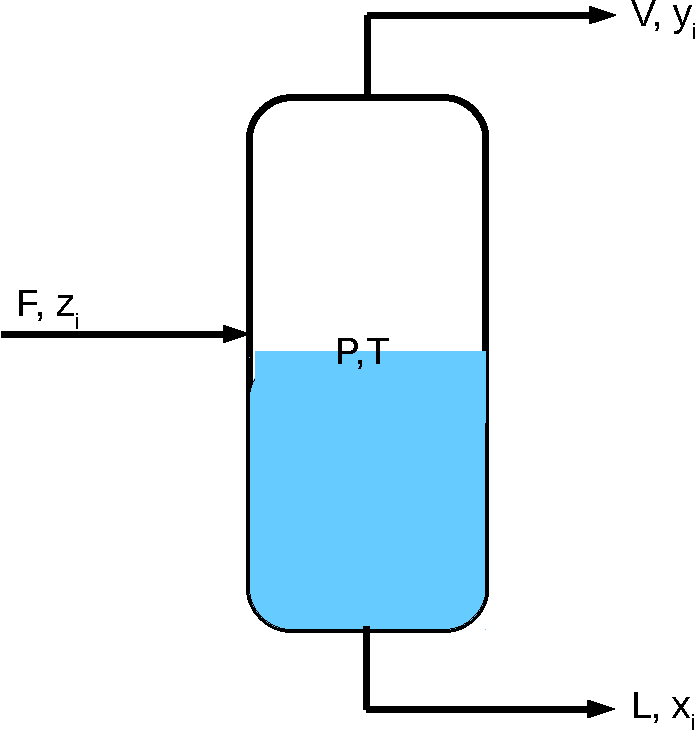
\includegraphics[width=.4\textwidth,clip]{./Figs/FlashDistillation}
     \end{center}
     \caption{Schematic of a flash distillation process.}\label{Chapter:VLE:Fig:Fig06}
  \end{figure}
Flash distillation is a common process in chemical industry to obtain solutions with the required enrichment from a feed-stock. Figure~\ref{Chapter:VLE:Fig:Fig06} shows a schematic of this process, where a liquid stream (\ie with pressure equal to or larger than its bubble point pressure) with molar fraction $F$ and overall composition $z_{i}$ is injected into a separation vessel through a pressure reduction valve. The sudden reduction in pressure leads to partial evaporation (\ie {\it flash}) of the liquid feed resulting in the formation of a vapour and a liquid stream. Vapour and Liquid streams have molar fraction $V$ and $L$, respectively, with compositions of $y_{i}$ and $x_{i}$. 
  The overall mass balance of the system is
  \begin{displaymath}
     F = V + L,
  \end{displaymath}
  for convenience, let's assume $F$ as equal to unity, $F=1$. Similarly, the mass balance for each component $i$ is
  \begin{displaymath}
     z_{i}F = x_{i}L + y_{i}V = x_{i}\left(1-V\right) + y_{i}V.
  \end{displaymath}
  Replacing $x_{i} = \frc{y_{i}}{K_{i}}$ and $F=1$,
  \begin{displaymath}
     z_{i} = \frc{y_{i}}{K_{i}}\left(1-V\right) + y_{i}V \;\;\Longrightarrow \;\;y_{i} = \frc{z_{i}K_{i}}{1+V\left(K_{1}-1\right)}. 
  \end{displaymath}
  As $\summation[y_{i}]{i=1}{\mathcal{C}} = 1$,
         \begin{shaded}
           \begin{equation}
              \summation[\frc{z_{i}K_{i}}{1+V\left(K_{i}-1\right)}]{i=1}{\mathcal{C}} = 1.\label{Chapter:VLE:Eqn:PartialMolarProperties:FlashEquation} 
           \end{equation}
         \end{shaded}
         Solving a $P-T$ flash problem is to \underline{find $V$} that satisfies Eqn.~\ref{Chapter:VLE:Eqn:PartialMolarProperties:FlashEquation}.

  \medskip
   % Example
   \begin{MyExample}{\begin{center}{\bf Example}\end{center}}
     \begin{example}\label{Chapter:VLE:Example5}\citep{Sandler_Book}
       A liquid mixture of 25 mol-$\%$ n-pentane $\left(nC_{5}\right)$, 45 mol-$\%$ n-hexane $\left(nC_{6}\right)$ and 30 mol-$\%$ n-heptane $\left(nC_{7}\right)$ initially at 69$^{\circ}$C and a high pressure, is partially vaporised by isothermically lowering the pressure to  1.013 bar. Calculate the relative amounts of vapour and liquid in equilibrium and compositions.
     \end{example}

% SOLUTION
     \noindent{\bf Solution:}
     This is a typical {\it flash} problem that can be described by Fig.~\ref{Chapter:VLE:Fig:Fig06}. From the given $P_{i}^{\text{sat}}$ relation at 69$^{\circ}$C,
   \begin{displaymath}
        \begin{cases}
            P_{5}^{\text{sat}} = 2.721 \text{ bar},\\ 
            P_{6}^{\text{sat}} = 1.024 \text{ bar},\\
            P_{7}^{\text{sat}} = 0.389 \text{ bar}.
        \end{cases}
   \end{displaymath}
Assuming ideal solution, $K_{i}$ for the three hydrocarbons can be readily obtained,
   \begin{displaymath}
        K_{i} = \frc{P_{i}^{\text{sat}}}{P} = \frc{y_{i}}{x_{i}},
          \begin{cases}
             K_{5} = 2.6861; \\
             K_{6} = 1.0109; \\
             K_{7} = 0.3840
          \end{cases}
   \end{displaymath}
   Therefore,
   \begin{displaymath}
       y_{5} = x_{5}K_{5},\;\;\;y_{6} = x_{6}K_{6},\;\;\;y_{7} = x_{7}K_{7},
   \end{displaymath}
    with the molar fraction constraints,
    \begin{displaymath}
        \begin{cases}
            x_{5}+x_{6}+x_{7} = 1,\\ 
            y_{5}+y_{6}+y_{7} = 1, \\
            F = V + L
        \end{cases}
   \end{displaymath}
   Assuming $F=1$, the mass balance of the individual components in equilibrium are
    \begin{displaymath}
        \begin{cases}
            x_{5}L + y_{5}V = z_{5} = 0.25 \\
            x_{6}L + y_{6}V = z_{6} = 0.45 \\
            x_{7}L + y_{7}V = z_{7} = 0.30            
        \end{cases}
   \end{displaymath}
   these relation can be rewritten as $\left(\text{based on }y_{5}+y_{6}+y_{7} = 1,\; y_{i}=K_{i}x_{i} \;\text{ and } V= 1-L\right)$
    \begin{displaymath}
        \begin{cases}
            x_{5}L + y_{5}V = z_{5} = 0.25 \;\Longrightarrow\; x_{5}\left[L\left(1-K_{5}\right)+K_{5}\right] = 0.25 \\
            x_{6}L + y_{6}V = z_{6} = 0.45 \;\Longrightarrow\; x_{6}\left[L\left(1-K_{6}\right)+K_{6}\right] = 0.45 \\
            x_{7}L + y_{7}V = z_{7} = 0.30 \;\Longrightarrow\; x_{7}\left[L\left(1-K_{7}\right)+K_{7}\right] = 0.30
        \end{cases}
   \end{displaymath}
   Now the molar fraction constraint of the liquid phase $x_{5}+x_{6}+x_{7} = 1$, is
   \begin{displaymath}
        \frc{0.25}{L\left(1-K_{5}\right)+K_{5}} + \frc{0.45}{L\left(1-K_{6}\right)+K_{6}} + \frc{0.30}{L\left(1-K_{7}\right)+K_{7}} = 1
   \end{displaymath}
   This expression has just one unknown, $L$, as a cubic polynomial. Solving with initial guess $L^{\text{guess}}=0.50$ leads to $L=0.5748$.  Now using 
    \begin{displaymath}
        \begin{cases}
            x_{5}L + y_{5}V = z_{5} = 0.25 \;\Longrightarrow\; x_{5}\left[L\left(1-K_{5}\right)+K_{5}\right] = 0.25  \;\Longrightarrow\;  x_{5} = 0.1456 \\
            x_{6}L + y_{6}V = z_{6} = 0.45 \;\Longrightarrow\; x_{6}\left[L\left(1-K_{6}\right)+K_{6}\right] = 0.45  \;\Longrightarrow\;  x_{6} = 0.4479 \\
            x_{7}L + y_{7}V = z_{7} = 0.30 \;\Longrightarrow\; x_{7}\left[L\left(1-K_{7}\right)+K_{7}\right] = 0.30  \;\Longrightarrow\;  x_{7} = 0.4065 
        \end{cases}
   \end{displaymath}
   leading to $\summation[x_{i}]{i}{} = 1.0000$. Molar fraction of the vapour phase is $V= 1-L=0.4252$, resulting in
    \begin{displaymath}
        \begin{cases}
            y_{5} = K_{5}x_{5} \;\Longrightarrow\; y_{5} = 0.3911 \\
            y_{6} = K_{6}x_{6} \;\Longrightarrow\; y_{6} = 0.4528 \\
            y_{7} = K_{7}x_{7} \;\Longrightarrow\; y_{7} = 0.1561 
        \end{cases}
   \end{displaymath}
    with $\summation[y_{i}]{i}{} = 1.0000$
   \end{MyExample}
   

\clearpage   
\begin{FinalSummaryBlock}{Summary}
     Concepts introduced in this chapter are relatively simple but far reaching. They are cornerstone for the remaining of this notes and for fundamental chemical thermodynamics. An extension of total derivative to multi-component systems led to the equilibrium criteria for general multiphase ($\mathcal{P}\ge2$) and multi-component ($\mathcal{C}\ge2$) mixtures.
    \begin{itemize}
       \item Initial definition and discussion of excess properties (Eqn.~\ref{Chapter:VLE:Eqn:ExcessProperties1a});
       \item Definition of chemical potential as the partial molar Gibbs free energy (Eqn.~\ref{Chapter:VLE:Eqn:ChemPotentialDef1b}) and development of a fundamental relation for multi-component systems (Eqn.~\ref{Chapter:VLE:Eqn:ChemPotentialDef1d});
       \item Chemical equilibrium can be assessed \wrt thermodynamic conditions as stated in Table~\ref{Chapter:VLE:Table:TableEquilibriumCriteria};
       \item In closed systems at constant pressure and temperature conditions, the criterion for equilibrium is that the Gibbs free energy is the minimum which leads to equality of chemical potential of each component at all phases (Eqn.~\ref{Chapter:VLE:EqnChemPotentialDef1c3});
       \item Multi-component VLE problems (\ie $\mathcal{C}\ge 2$ and $\mathcal{P}=2$) can be represented by $P-T-x_{i}y_{i}$ phase diagrams, where critical pressure and temperature (for individual components and the mixtures), liquid and vapour saturation lines, bubble and dew points can be identified;
       \item Although compositions, temperatures and pressures can be obtained from graphical representation (2-/3-D) of phase equilibrium, this is not very convenient and numerical models were develop to represent the partition of components in both phases in equilibrium;
       \item Raoult's law (Eqn.~\ref{Chapter:VLE:Eqn:RaoultLaw}) is an idealisation of the components' partition between vapour and liquid phases assuming limited molecular forces (\eg attractive and repulsive) act in the liquid phase;
       \item Henry's law (Eqn.~\ref{Chapter:VLE:Eqn:HenryLaw}) is applied to gases solubilised at low concentrations in liquid solutions;
       \item K-value models (Eqn.~\ref{Chapter:VLE:Eqn:KValue}) were mostly developed for petro-chemical industry to help quickly assess concentrations of (light) hydrocarbons in vapour and liquid phases;
       \item Dew and bubble coordinates (pressure, temperature and compositions) in typical industrial applications are discussed in Section~\ref{Chapter:VLE:Section:IndApplications};
       \item Depending on known conditions, four main problems may arise:
\begin{center}
   \begin{tabular}{|l c c|}
      \hline 
      $\mathbf{VLE}$ {\bf Problem} & {\bf Specified Variables} &  {\bf Computed Variables} \\  
      \hline
          {\bf Bubble Pressure}        &  $T$ and $x_{i}$           &   $P$ and $y_{i}$          \\
          {\bf Dew Pressure}           &  $T$ and $y_{i}$           &   $P$ and $x_{i}$          \\
          {\bf Bubble Temperature}     &  $P$ and $x_{i}$           &   $T$ and $y_{i}$          \\
          {\bf Dew Temperature}        &  $P$ and $y_{i}$           &   $T$ and $x_{i}$          \\     
      \hline
   \end{tabular}
\end{center}
    \end{itemize}
\end{FinalSummaryBlock}


%\part{Liquid Solutions}
%  \chapter{Solution Thermodynamics}\label{Chapter:SolutionThermodynamics}


   \begin{LearningObjectivesBlock}{Learning Objectives}
      Upon completion of this chapter, you will be able to
        \begin{enumerate}
           \item 
        \end{enumerate}
\medskip
     Recommended reading: Chapters 11-12 of \citet{SmithVanNess_Book}, 9-10 of \cite{Sandler_Book}, 6 \citet{Lue_Book}, 11 of \citet{Elliot_Book} or 5 of \citet{Atkins_Book}.
   \end{LearningObjectivesBlock}


%%%%%%%%%%%%%%%%%%%%%%%%%%%%%%%%%%%%%%%%%%%%%%%%%%%%%%%%%%%%%%%%%
\begin{comment}
   \begin{LearningObjectivesBlock}{Learning Objectives}
      Upon completion of this chapter, you will be able to
        \begin{enumerate}
           \item {\bf Knowledge:} Define, Name, Select, State 
           \item {\bf Comprehension:} Describe, Identify, Discuss
           \item {\bf Application:} Apply, Demonstrate, Employ, Sketch
           \item {\bf Analysis:} Analyse, Compare, Calculate, Solve
           \item {\bf Synthesis:} Determine, Formulate
           \item {\bf Evaluation:} Assess, Check, Estimate, Compare, Measure, Monitor
        \end{enumerate}
\end{comment}
%%%%%%%%%%%%%%%%%%%%%%%%%%%%%%%%%%%%%%%%%%%%%%%%%%%%%%%%%%%%%%%%%

%%%% ETOC
\localtableofcontents
   


%%% SUBSECTION
\section{Introduction}\label{Chapter:SolutionThermodynamics:Section:Introduction}
Vapour-liquid equilibrium of pure components and mixtures were the focus of study in Chapters~\ref{Chapter:VolumetricPropertiesPureSubstances}-\ref{Chapter:VLE}. In these chapters, equations of state were introduced to represent the $PVT$ behaviour of pure components in both vapour and liquid phases. From your readings, you may have noticed that EOS are largely applied, with relatively accuracy, to vapour phases, but rarely used to assess liquid phase behaviour. 

This is mainly due to the fact that EOS were originally (and cubic EOS in particular) to represent weak inter-molecular forces between gaseous molecules at relatively large distances (\ie {\it mean free path}). As pressure increases $\left(P\rightarrow \infty\right)$ and the distance between molecules tends to zero $\left(d\rightarrow 0\right)$, the accuracy of equations of state to predict $PVT$ behaviour also decreases, as the attractive and repulsive forces between molecules become stronger. 

Molecules in liquid phase are held together at close distances by strong attractive forces, however these forces are not strong enough to keep them in fixed positions (as inter-/intra-molecular forces in the solid phase) and the molecules are free to move past, slide over and collide with other molecules. A fraction of the molecules (mostly with higher energy) may be able to break such attractive forces and `escape' towards the vapour phase. 

Kinetic energy in gaseous molecules are larger than the attractive forces, leading to large distances between molecules and a tendency to occupy the whole volume of the system. The large kinetic energy in gaseous molecules also lead to continuous collisions between molecules and with the system (container) walls. During collisions, although total momentum is conserved, individual energies (and velocities) may decrease and molecules may move to a system with lower kinetic energy, \ie liquid phase.

\bigskip

In Chapter~\ref{Chapter:Introduction}, the concept of {\it mechanical} (\ie system at constant or uniform pressure) and {\it thermal} (from the Zeroth law) equilibrium were introduced. In order to define phase equilibria, we established (in Chapter~\ref{Chapter:ThermodynamicPropertiesPureFluids}) that an additional condition was necessary, {\it chemical equilibrium}, \ie equality of Gibbs free energy of all phases (Section~\ref{Chapter:ThermodynamicPropertiesPureFluids:Section:ClapeyronRelations}) for pure fluids. This concept can be extended for mixtures by using the definition of {\it chemical potential}, $\mu_{i}$ (Eqn.~\ref{Chapter:VLE:Eqn:ChemPotentialDef1b}),\index{Chemical potential}
         \begin{displaymath}
            \mu_{i} = \Partial[(nG)]{n_{i}}{T,P,n_{j\ne i}} \;\;\Longleftrightarrow\;\; \mu_{i} = \overline{G}_{i},
         \end{displaymath}
where $\overline{G}_{i}$ is the {\it partial molar Gibbs free energy}. This leads to the final phase equilibria condition in which {\it the chemical potential for each component at all coexisting phases are identical}, \ie 
         \begin{displaymath}
           \mfr[\mu]{i}{\alpha} = \mfr[\mu]{i}{\beta} = \cdots =  \mfr[\mu]{i}{j} = \cdots = \mfr[\mu]{i}{\mathcal{N}_{\mathcal{P}}}, \hspace{1.5cm} \forall i\in\{1,2,\cdots,\mathcal{C}\}\;\; \text{ and }\;\;\; \forall j\in\{\alpha,\beta,\cdots,\mathcal{N}_{\mathcal{P}}\}
         \end{displaymath}
         or for VLE systems:
         \begin{displaymath}
           \mfr[\mu]{i}{L} = \mfr[\mu]{i}{V},\;\;\;\forall i\in\{1,2,\cdots,\mathcal{C}\}
         \end{displaymath}

\medskip

The main assumptions for ideal gas behaviour assume that molecules of gas are massless particles with no interaction between them (\ie volume of the molecules is negligibly small compared with the volume occupied by the gas or simply the distance between gaseous molecules are often infinitely large, $d\rightarrow \infty$), except during elastic collisions over negligible duration. These conditions can only be met by fluids at sufficiently high temperature and relatively low pressure when large distances between molecules and high velocity overcome any interaction. The concept of ideality for liquids also exists and is based on the assumption that inter-molecular forces are the same between all molecules in solution. This assumption may be correct for pure non-polar substances (\ie in solutions with no major inter-/intra-molecular forces).

Thus, the aim of this Chapter is to define thermodynamic properties of real solutions based on properties of ideal solutions. Excess properties (Section~\ref{Chapter:VLE:Section:ExcessProperties}) plays a role similar to that of residual properties (Section~\ref{Chapter:ThermodynamicPropertiesPureFluids:Section:ResidualProperties}) for gases. In order to study solution properties at low to moderate pressures, {\it activity coefficient}, based on the definition of {\it fugacity}, is used. The {\it activity coefficient}, derived from the {\it excess Gibbs free energy}, is a measure of the extent of non-ideality of a real solution and helps describing phase equilibria of mixtures at low and moderate pressures.


%%% SECTION
\section{Fugacity}\label{Chapter:SolutionThermodynamics:Section:FugacitySection}\index{Fugacity}
\begin{subequations}
  A formal definition for {\it partial molar property} was introduced in Section~\ref{Chapter:VLE:Section:PartialMolarProperties} for an arbitrary extensive function $M$, Eqn.~\ref{Chapter:VLE:Eqn:PartialProperties2}. Such formulation was applied to the Gibbs free energy of a system with $n=n_{1}+n_{2}+\cdots+n_{\mathcal{C}}$ moles leading to the definition of the {\it chemical potential}, Eqns.~\ref{Chapter:VLE:Eqn:ChemPotentialDef1}-\ref{Chapter:VLE:Eqn:ChemPotentialDef1b},
  \begin{shaded}
     \begin{eqnarray}
       && dG = \Partial[G]{P}{T,n}dP + \Partial[G]{T}{P,n}dT + \underbrace{\Partial[G]{n}{T,P}}_{\mu}dn, \nonumber \\
       && \mu_{i} = \Partial[(nG)]{n_{i}}{T,P,n_{j\ne i}} \;\;\Longleftrightarrow\;\; \mu_{i} = \overline{G}_{i}, \nonumber
     \end{eqnarray}
  \end{shaded}
  \noindent For pure components,
  \begin{displaymath}
    G = n\mu \;\;\rightarrow \mu=\frc{G}{n}=\overline{g},
  \end{displaymath}
  where $\overline{g}$ is the molar Gibbs free energy. Using the Maxwell relation, Eqn.~\ref{Chapter:ThermodynamicPropertiesPureFluids:Eqn:MaxwellRelation7},
  \begin{eqnarray}
    && \Partial[G]{P}{T} = V = \Partial[n\mu]{P}{T} = n\Partial[\mu]{P}{T} \nonumber \\
    && \Partial[\mu]{P}{T} = \frc{V}{n} = \overline{v}\label{Chapter:SolutionThermodynamics:Eqn:fugacity1}
  \end{eqnarray}
  where $\underline{v}$ is the molar volume. For an ideal gas,
  \begin{displaymath}
     \Partial[\mu^{\text{ig}}]{P}{T} = \frc{RT}{P},
  \end{displaymath}
  where the superscript {\it ig} refers to ideal gas. This differential can be integrated as,
  \begin{equation}
    \mu^{\text{ig}} = RT\ln{P} + C(T),\label{Chapter:SolutionThermodynamics:Eqn:fugacity1a}
  \end{equation}
  where $C(T)$ is an integration constant. At limiting conditions, $P\rightarrow 0$ and $P\rightarrow\infty$, the chemical potential lies within $-\infty < \mu < +\infty$.
  \begin{shaded}
    \noindent For a fluid to be considered an ideal gas, pressure needs to be relatively low, thus we can use Eqn.~\ref{Chapter:SolutionThermodynamics:Eqn:fugacity1a} to represent the \underline{chemical potential of real fluids},
  \begin{equation}
    \mu = RT\ln{f} + C(T),\label{Chapter:SolutionThermodynamics:Eqn:fugacity1b}
  \end{equation}
  where $f$ is the {\it fugacity of a real gas}, \ie \blue{a representation of the pressure of an ideal gas that has the same chemical potential as the real gas.}
  \end{shaded}
  \noindent Since the {\it fugacity} has the \underline{units of pressure}, it is often referred as a `fictitious pressure'.  The definition of fugacity from Eqn.~\ref{Chapter:SolutionThermodynamics:Eqn:fugacity1b} is entirely general and can be readily extended to both liquids and solids. Now, replacing Eqn.~\ref{Chapter:SolutionThermodynamics:Eqn:fugacity1b} in the Maxwell relation, Eqn.~\ref{Chapter:ThermodynamicPropertiesPureFluids:Eqn:MaxwellRelation7}, at constant temperature,
  \begin{equation}
    RT\Partial[\left(\ln{f}\right)]{P}{T} = \overline{v}.\label{Chapter:SolutionThermodynamics:Eqn:fugacity1c}
  \end{equation}
  {\it Fugacity} can be obtained by integrating this equation holding $T$ constant. As pressure tends to zero (lower limit of the left-hand-side integration), the fluid behaves as an ideal gas. We can thus state that the fugacity of a pure component is equal to the pressure in the limit of zero pressure, \ie
      \begin{shaded}
        \begin{equation}
           \lim\limits_{P \rightarrow 0} \frc{f}{P} = 1.\label{Chapter:SolutionThermodynamics:Eqn:fugacity1d}
        \end{equation}
      \end{shaded}

  \noindent  In a \underline{mixture} containing $n$ moles of $\mathcal{C}$ chemical species, Eqn.~\ref{Chapter:SolutionThermodynamics:Eqn:fugacity1c} becomes,
      \begin{eqnarray}
        && RT\Partial[\left(\ln{f_{i}}\right)]{P}{T,n} = \overline{v}_{i},\;\;\;\;\forall i\in\left\{1,2,\cdots,\mathcal{C}\right\}\label{Chapter:SolutionThermodynamics:Eqn:fugacity1e1} \\
        && RT\Partial[\left(\ln{\overline{f}_{i}}\right)]{P}{T,n} = \overline{V}_{i},\label{Chapter:SolutionThermodynamics:Eqn:fugacity1e2}
      \end{eqnarray}
      where $f_{i}$ is the {\it fugacity of pure component $i$} and $\overline{f}_{i}$ is the {\it fugacity of component $i$ in the mixture}. $\overline{v}_{i}$ and $\overline{V}_{i}$ are the molar volume of pure component $i$ and, of component $i$ in the mixture. If we subtract Eqn.~\ref{Chapter:SolutionThermodynamics:Eqn:fugacity1e1} from \ref{Chapter:SolutionThermodynamics:Eqn:fugacity1e2} and integrate the result from $P'$ to $P$ at constant $T$,
      \begin{displaymath}
        RT\Partial[\left(\ln{\frc{\overline{f}_{i}}{f_{i}}}\right)]{P}{T,n} = \overline{V}_{i} - \overline{v}_{i} \;\;\Longrightarrow \;\;  RT\left[\left.\ln{\left(\frc{\overline{f}_{i}}{f_{i}}\right)}\right|_{P'}^{P}\right] = \int\limits_{P'}^{P}\left(\overline{V}_{i} - \overline{v}_{i}\right)dP
      \end{displaymath}
      Assuming that $P'$ tends to $0$,
      \begin{equation}
        RT\left[\ln{\left(\frc{\overline{f}_{i}}{f_{i}}\right)} - \lim\limits_{P'\rightarrow 0}\ln\left(\frc{\overline{f}_{i}}{f_{i}}\right)\right] = \int\limits_{0}^{P}\left(\overline{V}_{i} - \overline{v}_{i}\right)dP.\label{Chapter:SolutionThermodynamics:Eqn:fugacity1f}
      \end{equation}
      When $P'\rightarrow 0$
      \begin{displaymath}
        \begin{cases}
          f_{i} \rightarrow P', \\
          \overline{f}_{i} \rightarrow y_{i}P',
        \end{cases}
      \end{displaymath}
      and the limiting term in the previous equation becomes,
      \begin{displaymath}
        \lim\limits_{P'\rightarrow 0}\ln\left(\frc{\overline{f}_{i}}{f_{i}}\right) \rightarrow \ln{\left(\frc{y_{i}P'}{P'}\right)} = \ln{y_{i}}
      \end{displaymath}
      Thus Eqn.~\ref{Chapter:SolutionThermodynamics:Eqn:fugacity1f} becomes,
        \begin{displaymath}
          RT\left[\ln{\left(\frc{\overline{f}_{i}}{f_{i}}\right)} - \ln{y_{i}}\right] = \int\limits_{0}^{P}\left(\overline{V}_{i} - \overline{v}_{i}\right)dP
        \end{displaymath}
      \begin{shaded}
        \begin{equation}
           RT\ln{\left(\frc{\overline{f}_{i}}{y_{i}f_{i}}\right)} = \int\limits_{0}^{P}\left(\overline{V}_{i} - \overline{v}_{i}\right)dP. \label{Chapter:SolutionThermodynamics:Eqn:fugacity1g}
        \end{equation}
      \end{shaded}
  \noindent This expression relates fugacity of a pure component $i$ and the fugacity of the same component $i$ in a mixture with $\mathcal{C}$ chemical components during continuous change in pressure. The term in brackets in the left-hand side represents the ratio between partial pressures between real and ideal fluids in a mixture.

  \bigskip
        
      For an ideal mixture of ideal gases, the partial pressure of species $i$ is the fugacity of component $i$ in the mixture, \ie
         \begin{displaymath}
            \mfr[\overline{f}]{i}{V} = y_{i}P = P_{i}.
         \end{displaymath}
      Now, for an ideal mixture of real fluids,
         \begin{displaymath}
            \mfr[\overline{f}]{i}{L} = x_{i}\mfr[f]{i}{L},
         \end{displaymath}
      \ie the fugacity of a component in a mixture is a function of the fugacity of the pure component.
      \begin{shaded}
         An \underline{ideal solution} is a mixture in which,
        \begin{equation}
          \mfr[\overline{f}]{i}{V} = y_{i}P = P_{i}\;\;\;\text{ and }\;\;\; \mfr[\overline{f}]{i}{L} = x_{i}\mfr[f]{i}{L}\label{Chapter:SolutionThermodynamics:Eqn:fugacity2a}
        \end{equation}
        These expressions are called {\it Lewis-Randall rules} and they describe relations between phase compositions and fugacities.\index{Lewis-Randall rules|see {Solutions}}\index{Solutions!Lewis-Randall rules}
      \end{shaded}
      
\end{subequations}

      
%%% SECTION
\section{Activity and Activity Coefficient }\label{Chapter:SolutionThermodynamics:Section:ActivitySection}.\index{Activity|see {Solutions}}\index{Solutions!Activity}\index{Activity coefficient|see {Solutions}}\index{Solutions!Activity coefficient}
   \begin{subequations}
        
      In a mixture (based on Eqn.~\ref{Chapter:SolutionThermodynamics:Eqn:fugacity1b}),
        \begin{displaymath}
           \mu_{i} = RT\ln{\overline{f}_{i}} + C_{i}(T),
        \end{displaymath}
      consider a reference-state, where a species $i$ of a multi-component system is pure at temperature $T$ and at reference-state pressure, $P_{\text{ref}}$,
        \begin{equation}
           \mu_{i} - \mu_{i}^{\circ} = RT\ln{\left(\frc{\overline{f}_{i}}{f_{i}^{\circ}}\right)},\label{Chapter:SolutionThermodynamics:Eqn:activity1a}
        \end{equation}
      where superscript $^{\circ}$ stands for {\it reference state}. 
        \begin{shaded}
           \noindent Now, we can define the term in brackets as the {\it activity} (dimensionless)
           \begin{equation}
              \frc{\overline{f}_{i}}{f_{i}^{\circ}} = a_{i}, \label{Chapter:SolutionThermodynamics:Eqn:activity1b}
           \end{equation}
           which `measures' the deviation from ideal behaviour.
        \end{shaded}
      \noindent Since $\mu^{\circ} = \overline{g}^{\circ}_{i}$, Eqn.~\ref{Chapter:SolutionThermodynamics:Eqn:activity1a} becomes
        \begin{equation}
           \mu_{i} = \overline{g}^{\circ}_{i} + RT\ln{a_{i}}\label{Chapter:SolutionThermodynamics:Eqn:activity1c}
        \end{equation}
      For an ideal solution, the {\it Lewis-Randall relation} can be used,
        \begin{displaymath}
           a_{i} =  \frc{\overline{f}_{i}}{f_{i}^{\circ}} = \frc{y_{i}f_{i}}{f_{i}^{\circ}},
        \end{displaymath}
      where $f_{i}$ is the fugacity of pure component $i$ at $P$ and $T$, and $f_{i}^{\circ}$ is the fugacity of pure component $i$ at $T$ and the reference-pressure $P_{\text{ref}}$. Thus,
        \begin{displaymath}
           \mu_{i} = \overline{g}^{\circ}_{i} + RT\ln{\left( \frc{y_{i}f_{i}}{f_{i}^{\circ}}\right)}.
        \end{displaymath}

        \begin{shaded}
            \noindent For \underline{\it ideal solutions},
              \begin{equation}
                 \mu_{i} = \overline{g}^{\circ}_{i} + RT\ln{\left[\left(\frc{f_{i}}{P}\right)\left(\frc{P_{\text{ref}}}{f_{i}^{\circ}}\right)\frc{y_{i}P}{P_{\text{ref}}}\right]}.\label{Chapter:SolutionThermodynamics:Eqn:activity1d}
              \end{equation}
            If component $i$ behaves as an \underline{\it ideal gas} at both $\left(T,P\right)$ and $\left(T,P_{\text{ref}}\right)$, thus $\frc{f_{i}}{P} = \frc{f_{i}^{\circ}}{P_{\text{ref}}}=1$ and Eqn.~\ref{Chapter:SolutionThermodynamics:Eqn:activity1d} becomes
              \begin{equation}
                 \mu_{i} = \overline{g}^{\circ}_{i} + RT\ln{\frc{y_{i}P}{P_{\text{ref}}}}.\label{Chapter:SolutionThermodynamics:Eqn:activity1e}
              \end{equation}
             This expression allows the calculation of the chemical potential of the vapour phase in a mixture subjected to a change in pressure based on composition and temperature. Molar Gibbs energy at reference conditions, $\overline{g}^{\circ}_{i}$, for several chemical species are often tabulated and can be found in any chemical engineering handbook.
\medskip
             
        \noindent Finally, we can now define the \underline{\blue{activity coefficient}}, $\gamma_{i}$, as
          \begin{equation}
              a_{i} = \frc{y_{i}f_{i}}{f_{i}^{\circ}}\;\;\;\;\Rightarrow \;\;\;\; \gamma_{i} = \frc{a_{i}}{y_{i}} = \frc{f_{i}}{f_{i}^{\circ}}\label{Chapter:SolutionThermodynamics:Eqn:activity1f}
          \end{equation}
         And for solutions,
          \begin{equation}
              \gamma_{i} = \frc{\overline{f}_{i}}{x_{i}f_{i}}\label{Chapter:SolutionThermodynamics:Eqn:activity1g}
          \end{equation}
         The \underline{\blue{activity coefficient}} takes into account non-idealities in the liquid phase. Now, we can properly define the \underline{Raoult's law} (Section~\ref{Chapter:VLE:Section:RaoultsLaw}) at low pressure,\index{Solutions!Raoult's law}
          \begin{equation}
               \gamma_{i} = \frc{\overline{f}_{i}}{x_{i}f_{i}} = \frc{y_{i}P}{x_{i}f_{i}}=\frc{y_{i}P}{x_{i}P_{i}^{\text{sat}}} \;\;\;\Longrightarrow \;\;\;\ x_{i}\gamma_{i}P_{i}^{\text{sat}} = y_{i}P \label{Chapter:SolutionThermodynamics:Eqn:RaoultLaw}
          \end{equation}
          Equation~\ref{Chapter:SolutionThermodynamics:Eqn:RaoultLaw} is the general form for Raoult's law. If the solution is ideal, $\gamma_{i}=1$, Eqn.~\ref{Chapter:VLE:Eqn:RaoultLaw} is recovered.

      \end{shaded}       
%
   \end{subequations}

\begin{table}
   \begin{center}
      \begin{tabular}{l c l l l}
          \hline
             {\bf Components}   & {\bf Basis}  & {\bf Standard-state}   & {\bf Activity}        & {\bf Limits} \\
          \hdashline
             Solid or liquid    &              &  Pure                  & $a=1$                 &              \\
          \hdashline
             Solvent            &   Raoult     &  Pure solvent          & $a\frc{P}{P^{\star}}$,  & $\gamma\rightarrow 1\text{ as } x\rightarrow 1$ \\
                                &              &                        & $a=\gamma x$          &  (pure solvent) \\
          \hdashline
             Solute             & Henry        & (1) hypothetical state of& $a=\frc{P}{\mathcal{H}}$,& $\gamma\rightarrow 1\text{ as } x\rightarrow 0$ \\
                                &              & pure solute            & $a=\gamma x$          &                                     \\
          \hdashline
                                &              & (2) hypothetical state of& $a=\gamma\frc{m}{m^{\circ}}$& $\gamma\rightarrow 1\text{ as } m\rightarrow 0$ \\
                                &              & solute at molality $m$   &                     &                                     \\
         \hline 
       \end{tabular}
       \caption{Standard states for activity \citep[extracted from][]{Atkins_Book}.}\label{Chapter:SolutionThermodynamics:Table:StandarStateActivity}
   \end{center}
\end{table}
      
%%% SECTION
\section{Henry's Law}\label{Chapter:SolutionThermodynamics:Section:HenryLaw}\index{Solutions!Henry's law}
Now that the concepts of fugacity and activity coefficient were introduced, we can return to the special VLE condition in which the solute is very diluted in the mixture (Section~\ref{Chapter:VLE:Section:HenryLaw}). In such cases, the fugacity of a very dilute chemical species in a liquid mixture (\eg dissolved gases or solid of limited solubility) is experimentally found to be a linear function of its low composition (\ie mole fraction)\footnote{It is clear that the division in the limiting term,
  \begin{displaymath}
    \lim\limits_{x_{i}\rightarrow 0}\frc{\overline{f_{i}}}{x_{i}}
  \end{displaymath}
  is undetermined as $f_{i}=0\text{ when }x_{i}\rightarrow 0$, \ie at infinite dilution of a solute $i$ in solution, the fugacity of this component is null. In order to solve this mathematical problem, we can use the L'H\^opital rule (see Appendix~\ref{Appendix:lHopital}) which states that for a limit,
         \begin{displaymath}
                 \lim\limits_{x\rightarrow a}\frc{f(x)}{g(x)},
         \end{displaymath}
         if the numerator and denominator are finite at $a$, and $g(a)=0$, then
         \begin{displaymath}
                 \lim\limits_{x\rightarrow a}\frc{f(x)}{g(x)} =  \lim\limits_{x\rightarrow a}\frc{f'(a)}{g'(a)}.
         \end{displaymath}
         Therefore, the limiting dilution case can be solved as
         \begin{displaymath}
                 \lim\limits_{x_{i}\rightarrow 0}\frc{\overline{f_{i}}}{x_{i}} = \left(\frc{d \overline{f_{i}}}{d x_{i}}\right)_{x_{i}=0},
         \end{displaymath}
}, \ie   
      \begin{eqnarray}
        && \lim\limits_{x_{i}\rightarrow 0}\frc{\overline{f_{i}}}{x_{i}} = \left(\frc{d \overline{f_{i}}}{d x_{i}}\right)_{x_{i}=0}  \equiv \mathcal{H}_{i}, \nonumber \\
        && \mfr[\overline{f}]{i}{L}(T,P,x) = x_{i}\mathcal{H}_{i}(T,P)\;\;\;\;\text{ as } x_{i}\rightarrow 0.
      \end{eqnarray}      
This proportionality constant, $\mathcal{H}$, is called {\it Henry's law constant}, and is dependent on the solute-solvent pair, temperature and pressure. This experimentally-defined constant was first introduced in Eqn.~\ref{Chapter:VLE:Section:HenryLaw} as, in equilibrium conditions (at $P$, $T$ and $n$ constants), $\mfr[\overline{f}]{i}{V}=\mfr[\overline{f}]{i}{L}$,
         \begin{shaded}
           \begin{displaymath}
             P_{i} = y_{i}P = x_{i}\mathcal{H}_{i},
           \end{displaymath}
           with $\mfr[\overline{f}]{i}{V}=y_{i}P$.
        \end{shaded}
%

      
%%% SECTION
\section{Gibbs-Duhem Equation}\label{Chapter:SolutionThermodynamics:Section:GibbsDuhem}
   \begin{subequations}
%
       In Section~\ref{Section:04:PartialMolarProperties}, the concept of \underline{\it partial molar property} of species $i$ in solution was defined as
         \begin{displaymath}
            \overline{M}_{i} = \Partial[(nM)]{n_{i}}{T,P,n_{j\ne i}},
         \end{displaymath}
        \ie the change of the total property $nM$ of a mixture of $\mathcal{C}$ species resulting from the addition at constant $T$ and $P$ of infinitesimal amount of species $i$ to a prescribed amount of solution.  It is important to bear in mind that \underline{\it partial molar property} of a substance is different from {\it molar property} of the same substance in a pure state at the same $T$ and $P$. This is due to inter-/intra-molecular forces that imposes interactions between species in solution.
\medskip

      Equation~\ref{Mod04_PartialProperties2} is a general expression for the change of any extensive property, $M$
         \begin{displaymath}
            d(nM) = n\Partial[M]{P}{T,x}dP + n\Partial[M]{T}{P,x}dT + \summation[\overline{M}_{i}dn_{i}]{i}{}.
         \end{displaymath}
      Mole fraction of a species $i$ was also introduced in Section~\ref{Section:04:Compositions} as,
         \begin{displaymath}
            x_{i} = \frc{n_{i}}{n} \;\;\Rightarrow\;\; n_{i} = x_{i}n,
         \end{displaymath}
      Applying {\it derivative of a product} rule on $n_{i}$,
         \begin{displaymath}
             dn_{i} = x_{i}dn + n dx_{i},
         \end{displaymath}
      and for the total property $(nM)$,
         \begin{displaymath}
             d(nM) = n d M + M dn.
         \end{displaymath}
      Replacing these expressions in Eqn.~\ref{Mod04_PartialProperties2},
        \begin{displaymath}
           n d M + M d n = n \Partial[M]{T}{P,x}dT + n\Partial[M]{P}{T,x}dP + \summation[\overline{M}_{i}\left(x_{i}dn + ndx_{i}\right)]{i}{}
        \end{displaymath}
      Rearranging this expression,
        \begin{equation}
           \underbrace{\left[dM - \Partial[M]{T}{P,x}dT - \Partial[M]{P}{T,x}dP - \summation[\overline{M}_{i}dx_{i}]{i}{}\right]}_{A}n + \underbrace{\left[M-\summation[\overline{M}_{i}x_{i}]{i}{}\right]}_{B}dn = 0\label{Chapter:SolutionThermodynamics:Eqn:GibbsDuhem1a}
        \end{equation}
      Equation~\ref{Chapter:SolutionThermodynamics:Eqn:GibbsDuhem1a} is valid for any arbitrary values of $n$ and $dn$, therefore $n$ and $dn$ should be independent of each other. Thus, this expression is only true if the coefficients $A$ and $B$ are zero, \ie
          \begin{eqnarray}
              A &=& dM - \Partial[M]{T}{P,x}dT - \Partial[M]{P}{T,x}dP - \summation[\overline{M}_{i}dx_{i}]{i}{} = 0 \nonumber \\
              dM &=& \Partial[M]{T}{P,x}dT + \Partial[M]{P}{T,x}dP + \summation[\overline{M}_{i}dx_{i}]{i}{}, \label{Chapter:SolutionThermodynamics:Eqn:GibbsDuhem1b}
          \end{eqnarray}
      and
          \begin{eqnarray}
              B &=& M-\summation[\overline{M}_{i}x_{i}]{i}{} = 0 \nonumber \\
              M &=& \summation[\overline{M}_{i}x_{i}]{i}{}\label{Chapter:SolutionThermodynamics:Eqn:GibbsDuhem1c} \\
             \text{as } nM = n\summation[\overline{M}_{i}x_{i}]{i}{} &\Rightarrow& dM = \summation[x_{i}d \overline{M}_{i}]{i}{} + \summation[\overline{M}_{i}dx_{i}]{i}{}\label{Chapter:SolutionThermodynamics:Eqn:GibbsDuhem1d}
          \end{eqnarray}
      Replacing Eqn.~\ref{Chapter:SolutionThermodynamics:Eqn:GibbsDuhem1d} in Eqn.~\ref{Chapter:SolutionThermodynamics:Eqn:GibbsDuhem1b} leads to the \blue{\it Gibbs-Duhem Equation (GDE)},
          \begin{shaded}
             \begin{equation}
                 \Partial[M]{T}{P,x}dT + \Partial[M]{P}{T,x}dP - \summation[x_{i}d\overline{M}_{i}]{i}{} = 0.\label{Chapter:SolutionThermodynamics:Eqn:GibbsDuhem1e}
             \end{equation}
             The \blue{GDE} must be satisfied for all changes in $P$, $T$ and $\overline{M}_{i}$.
          \medskip

             \noindent For changes at constant temperature and pressure conditions, the \blue{GDE} becomes
               \begin{equation}
                   \summation[x_{i}d\overline{M}_{i}]{i}{} = 0.\label{Chapter:SolutionThermodynamics:Eqn:GibbsDuhem1f}
               \end{equation}
             Or taking any arbitrary species $j$,
               \begin{equation}
                   \summation[x_{i}\frc{d\overline{M}_{i}}{dx_{j}}]{i}{} = 0, \;\;\;\text{ at constant } T\text{ and } P.\label{Chapter:SolutionThermodynamics:Eqn:GibbsDuhem1g}
               \end{equation}
             Equations~\ref{Chapter:SolutionThermodynamics:Eqn:GibbsDuhem1f}-\ref{Chapter:SolutionThermodynamics:Eqn:GibbsDuhem1g} imply that partial molar properties of various species, $\overline{M}_{i}$, are \underline{not} independent. 

             \noindent Some key-properties,
               \begin{displaymath}
                   \begin{cases}
                       \lim\limits_{x_{i}\rightarrow 0}\overline{M}_{i} = \overline{M}_{i}^{\infty} & \text{\ie at infinite dilutions;} \\
                       \lim\limits_{x_{i}\rightarrow 1}\overline{M}_{i} = M_{i}                   & \text{ \ie nearly pure chemical species.} 
                   \end{cases}
               \end{displaymath}
          \end{shaded}
%
   \end{subequations}


      
%%% SECTION
\section{Partial Molar Properties in Binary Solutions}\label{Chapter:SolutionThermodynamics:PMP_Binary}
   \begin{subequations}
%
       In a mixture with $n$ moles, we can define the {\it isothermal molar property change of mixing}, $\Delta M_{\text{mix}}$ as,
          \begin{eqnarray}
              \Delta M_{\text{mix}}(T,P) & = & M(T,P) - \summation[x_{i}M_{i}(T,P)]{i}{} \nonumber \\
                                      &=& \underbrace{\summation[\overline{M}_{i}x_{i}]{i}{}}_{\text{from Eqn.~\ref{Chapter:SolutionThermodynamics:Eqn:GibbsDuhem1c}}} - \summation[x_{i}M_{i}]{i}{} \nonumber \\
                                      &=& \summation[x_{i}\left(\overline{M}_{i}-M_{i}\right)]{i}{}.\label{Chapter:SolutionThermodynamics:Eqn:GibbsDuhem1h}
          \end{eqnarray}
       In a \underline{binary system} (from Eqn.~\ref{Chapter:SolutionThermodynamics:Eqn:GibbsDuhem1c}),
          \begin{equation}
              M = \overline{M}_{1} x_{1} + \overline{M}_{2} x_{2},\;\;\;\;\;\left(\text{at constant }P \text{ and } T\right),\label{Chapter:SolutionThermodynamics:Eqn:GibbsDuhem1i}
          \end{equation}
      and using the {\it derivative of a product} rule on $M$,
          \begin{displaymath}
              dM = \left(x_{1}d\overline{M}_{1} + \overline{M}_{1}dx_{1}\right) + \left(x_{2}d\overline{M}_{2} + \overline{M}_{2}dx_{2}\right), 
          \end{displaymath}
      applying GDE (Eqn.~\ref{Chapter:SolutionThermodynamics:Eqn:GibbsDuhem1f}) in this expression, and using 
          \begin{displaymath}
             \summation[x_{i}]{i}{}=1\;\;\Leftrightarrow\;\; x_{1}+x_{2}=1\;\;\Rightarrow\;\;\; dx_{1}=-dx_{2},
          \end{displaymath}
      leads to 
          \begin{eqnarray}
             && \cancel{\red{x_{1}d\overline{M}_{1}}} + \overline{M}_{1}dx_{1} + \cancelto{\red{=0 \text{ (due to GDE, Eqn.~\ref{Chapter:SolutionThermodynamics:Eqn:GibbsDuhem1f})}}}{\red{x_{2}d\overline{M}_{2}}} - \overline{M}_{2}dx_{1} = dM \nonumber \\
             && dM = \overline{M}_{1}dx_{1} - \overline{M}_{2}dx_{1} \nonumber \\
             && \frc{dM}{dx_{1}} = \overline{M}_{1} - \overline{M}_{2} \label{Chapter:SolutionThermodynamics:Eqn:GibbsDuhem1j}
          \end{eqnarray}
          \begin{shaded}
             Using Eqn.~\ref{Chapter:SolutionThermodynamics:Eqn:GibbsDuhem1i} in Eqn.~\ref{Chapter:SolutionThermodynamics:Eqn:GibbsDuhem1j},
               \begin{eqnarray}
                  && \frc{dM}{dx_{1}} = \overline{M}_{1} - \left(\frc{M-\overline{M}_{1}x_{1}}{x_{2}}\right) \nonumber \\
                 && x_{2}\frc{dM}{dx_{1}} =  \underbrace{x_{2}\overline{M}_{1}}_{\left(1-x_{1}\right)\overline{M}_{1}} - M + \overline{M}_{1}x_{1} \nonumber
               \end{eqnarray}
               \begin{equation}
                 \begin{cases}
                    \overline{M}_{1} = M + x_{2}\frc{dM}{dx_{1}},\\% \label{Chapter:SolutionThermodynamics:Eqn:GibbsDuhem1k} \\
                    \overline{M}_{2} = M - x_{1}\frc{dM}{dx_{1}} \label{Chapter:SolutionThermodynamics:Eqn:GibbsDuhem1k}
                 \end{cases}
              \end{equation}
            In binary solutions, the partial molar properties can be easily calculated from these two  expressions as a function of composition at constant $T$ and $P$. %From the GDE,
              \begin{eqnarray}
                   && x_{1}d\overline{M}_{1} + x_{2}d\overline{M}_{2} = 0 \;\;\;\;\;\blue{\times\frc{1}{dx_{1}}} \nonumber \\
                   && x_{1}\frc{d\overline{M}_{1}}{dx_{1}} + x_{2}\frc{d\overline{M}_{2}}{dx_{1}} = 0 \;\;\;\;\;\blue{\times\frc{1}{x_{1}}}\nonumber \\ %\label{Chapter:SolutionThermodynamics:Eqn:GibbsDuhem1l} \\
                   && \frc{d\overline{M}_{1}}{dx_{1}} + \frc{x_{2}}{x_{1}}\frc{d\overline{M}_{2}}{dx_{1}} = 0. \label{Chapter:SolutionThermodynamics:Eqn:GibbsDuhem1l} 
              \end{eqnarray}
          \end{shaded}
 %
   \end{subequations}
      
%%% SECTION
\section{Ideal Gas Mixture Model}\label{Chapter:SolutionThermodynamics:IGM}
   \begin{subequations}
%
     Since Module~\ref{Section:01}, we have used the equation of state for {\it ideal gases},
     \begin{displaymath}
        PV = nRT \;\;\;\Rightarrow\;\;\; P\overline{v} = RT
     \end{displaymath}
     In an {\it ideal gas mixture} (igm), the EOS has a similar format,
     \begin{equation}
       PV^{\text{igm}} = \underbrace{\left(n_{1}+n_{2}+\cdots+n_{\mathcal{C}}\right)}_{N\text{ moles}}RT = \left(\summation[n_{i}]{i=1}{\mathcal{C}}\right)RT = NRT.\label{Chapter:SolutionThermodynamics:Eqn:IGM1} 
     \end{equation}
     The internal energy of the gaseous mixture, $U^{\text{igm}}$, is just the summation of the internal energies of the individual components of the mixture,
     \begin{equation}
       U^{\text{igm}}(T,N) = \summation[n_{i}\overline{u}_{i}^{\text{ig}}(T)]{i=1}{\mathcal{C}},\label{Chapter:SolutionThermodynamics:Eqn:IGM2} 
     \end{equation}
     where $\overline{u}_{i}^{\text{ig}}=\frac{U_{i}^{\text{ig}}}{n_{i}}$ is the molar internal energy.We can change the notation on Eqns.~\ref{Chapter:SolutionThermodynamics:Eqn:IGM1}-\ref{Chapter:SolutionThermodynamics:Eqn:IGM2} to replace the number of moles by molar fraction, $y_{i}$, of the gas mixture, and to obtain the {\it partial molar internal energy}, $\overline{U}_{i}^{\text{igm}}(T,y)$
     \begin{equation}
       \overline{U}_{i}^{\text{igm}}(T,y) = \Partial[U^{\text{igm}}(T,N)]{n_{i}}{T,P,n_{j\ne i}} = \left[\frc{\partial\summation[n_{j}\overline{u}_{j}^{\text{ig}}(T)]{j=1}{\mathcal{C}}}{\partial n_{i}}\right]_{T,P,n_{j\ne i}}  = \overline{u}_{i}^{\text{ig}}(T)\label{Chapter:SolutionThermodynamics:Eqn:IGM3}
     \end{equation} 
     This expression indicates that the partial molar internal energy of species $i$ in an ideal gas mixture at a given tempereature is equal to the pure component molar internal energy of that component behaving as an ideal gas at the same temperature. We can also obtain the {\it partial molar volume}, $\overline{V}_{i}^{\text{igm}}$, with the same conclusion,
     \begin{equation}
       \overline{V}_{i}^{\text{igm}}(T,P,y) = \Partial[V^{\text{igm}}(T,P,N)]{n_{i}}{T,P,n_{j\ne i}} = \left[\frc{\partial\summation[n_{j} \frc{RT}{P}]{j=1}{\mathcal{C}}}{\partial n_{i}}\right]_{T,P,n_{j\ne i}} = \frc{RT}{P} = \overline{v}_{i}^{\text{ig}}(T,P).\label{Chapter:SolutionThermodynamics:Eqn:IGM4}
     \end{equation}
     \medskip

     The partial pressure of species $i$ in a gas mixture, $P_{i}$ (see Dalton's law in Section~\ref{Section:04:RaoultsLaw}), is defined for both ideal and real gas mixtures as
     \begin{displaymath}
       P_{i} = y_{i}P,
     \end{displaymath}
     and for an ideal gas mixture,
     \begin{equation}
       P_{i}^{\text{igm}}(N,T,V,y) = \frc{n_{i}}{\summation[n_{j}]{j=1}{\mathcal{C}}}P = \frc{n_{i}}{\summation[n_{j}]{j=1}{\mathcal{C}}}\left[\summation[n_{j}\frc{RT}{V}]{j=1}{\mathcal{C}}\right] = \frc{n_{i}RT}{V} = P^{\text{ig}}\left(n_{i},V,T\right),\label{Chapter:SolutionThermodynamics:Eqn:IGM4}
     \end{equation}
     \ie for ideal gas mixtures, the partial pressure of species $i$ is equal to the pressure that would be exerted if the same number of moles of that species, $n_{i}$, alone were contained in the same volume, $V$, at $T$ and $P$. 
\medskip

     As there is {\bf no} effective inter-/intra-molecular interactions in an ideal gas mixture, the effect on each species of the mixture at constant $T$ and $P$ is equivalent to:
     \begin{itemize}
       \item reducing the pressure from $P$ to $P_{i}$, or;
       \item expanding each gas from its initial volume $V_{i}=n_{i}RT/P$ to $V=\summation[n_{i}RT/P]{}{}$.
     \end{itemize}
     Thus using the entropy relations below for ideal gases\footnote{These relations have not been derived in this Notes, but can be obtained assuming $S=S(T,P)$ and $S=S(T,V)$, definitions of coefficients of thermal expansion, $\beta$, and isothermal compressibility, $\kappa$, Eqn.~\ref{Mod02_Compressibilityexpansivity}, and Maxwell relations.},
       \begin{displaymath}
           dS =
         \begin{cases}
              C_{p}d\left(\ln{T}\right) - Rd\left(\ln{P}\right), \\
              C_{v}d\left(\ln{T}\right) + Rd\left(\ln{V}\right),
         \end{cases}          
     \end{displaymath}
     leading to (assuming constant $T$),
       \begin{displaymath}
           \overline{S}_{i}^{\text{igm}}(T,P,y) - \overline{s}_{i}^{\text{ig}}(T,P) =
         \begin{cases}
              -R\ln{\frc{P_{i}}{P}} = -R\ln{y_{i}}\;\;\;\text{ or }, \\
               R\ln{\frc{V}{V_{i}}} = R\ln{\frc{\summation[n_{j}RT/P]{j}{}}{n_{i}RT/P}} = -R\ln{y_{i}},
         \end{cases}          
     \end{displaymath}
     for the whole mixture, the molar entropy change of mixing, $\Delta_{\text{mix}}\overline{S}^{\text{igm}}$ (see Eqn.~\ref{Chapter:SolutionThermodynamics:Eqn:GibbsDuhem1h}) can be obtained from
     \begin{displaymath}
          \Delta_{\text{mix}}S^{\text{igm}} = \summation[n_{i}\left(\overline{S}_{i}^{\text{igm}}(T,P,y) - \overline{s}_{i}^{\text{ig}}(T,P) \right) ]{i=1}{\mathcal{C}} = -R\summation[n_{i}\ln{y_{i}}]{i=1}{\mathcal{C}}.
     \end{displaymath}
     If this expression is divided by the total number of moles, $\summation[n_{j}]{j=1}{\mathcal{C}}$,
     \begin{equation}
       \Delta_{\text{mix}}\overline{s}^{\text{igm}} = - R \summation[y_{i}\ln{y_{i}}]{i=1}{\mathcal{C}}.
     \end{equation}
\medskip
  
     \noindent With volume, internal energy and entropy change of mixing, partial molar properties of other thermodynamic potentials can be readily obtained. For enthalpy,
     \begin{eqnarray}
          && \overline{H}_{i}^{\text{igm}}(T,P,y) = \overline{h}_{i}^{\text{ig}}(T,P) \nonumber \\
          && \overline{H}^{\text{igm}}(T,P,y) = \summation[y_{i}\overline{h}_{i}^{\text{ig}}(T,P)]{i=1}{\mathcal{C}},
     \end{eqnarray}
     and for Gibbs free energy from $G=H-TS$,
     \begin{eqnarray}
       \overline{G}_{i}^{\text{igm}}(T,P,y) &=& \overline{H}_{i}^{\text{igm}}(T,P,y) - T\overline{S}_{i}^{\text{igm}}(T,P,y) \nonumber \\
                                        &=& \overline{h}_{i}^{\text{ig}}(T,P) - T\left[ \overline{s}_{i}^{\text{ig}}(T,P) - R\ln{y_{i}}\right] \nonumber \\
                                        &=& \overline{g}_{i}^{\text{ig}}(T,P) + RT\ln{y_{i}},
     \end{eqnarray}
     and the Gibbs free energy change of mixing,
     \begin{eqnarray}
        \Delta_{\text{mix}}\overline{g}_{i}^{\text{igm}} &=& \summation[y_{i}\left(\overline{G}_{i}^{\text{igm}}(T,P,y)-\overline{g}_{i}^{\text{ig}}(T,P)\right)]{i=1}{\mathcal{C}} \nonumber \\
                                        &=& RT\summation[y_{i}\ln{y_{i}}]{i=1}{\mathcal{C}} \nonumber 
     \end{eqnarray}


 \begin{table}\scriptsize
     \begin{tabular}{ | c | c | c | c |}%\scriptsize
 \hline
        {\bf Property}    &   {\bf Partial Molar}   &  {\bf Change of Mixing}                    &  {\bf Molar Property} \\
                          &   {\bf Property}        &  $\left(\mathbf{\Delta_{\text{mix}}}\right)$  &                       \\
 \hline
            Volume        &   $\overline{V}_{i}^{\text{igm}}(T,y) = \overline{v}_{i}^{\text{ig}}(T)$ & $\Delta_{\text{mix}} \overline{v}^{\text{igm}}=0 $ & $\overline{v}^{\text{igm}}(T,P,y) = \summation[y_{i}\overline{v}_{i}^{\text{ig}}(T,P)]{}{}$ \\
         Internal Energy  &   $\overline{U}_{i}^{\text{igm}}(T,y) = \overline{u}_{i}^{\text{ig}}(T)$ & $\Delta_{\text{mix}} \overline{u}^{\text{igm}}=0 $ & $\overline{u}^{\text{igm}}(T,y) = \summation[y_{i}\overline{u}_{i}^{\text{ig}}(T)]{}{}$ \\
         Enthalpy         &   $\overline{H}_{i}^{\text{igm}}(T,y) = \overline{h}_{i}^{\text{ig}}(T)$ & $\Delta_{\text{mix}} \overline{h}^{\text{igm}}=0 $ & $\overline{h}^{\text{igm}}(T,P,y) = \summation[y_{i}\overline{h}_{i}^{\text{ig}}(T,P)]{}{}$ \\
         Entropy          &   $\overline{S}_{i}^{\text{igm}}(T,P,y) = \overline{s}_{i}^{\text{ig}}(T,P)-R\ln{y_{i}}$ & $\Delta_{\text{mix}} \overline{s}^{\text{igm}}=-R\summation[y_{i}\ln{y_{i}}]{}{}$ & $\overline{s}^{\text{igm}}(T,P,y) = \summation[y_{i}\overline{s}_{i}^{\text{ig}}(T,P)]{}{}-R\summation[y_{i}\ln{y_{i}}]{}{}$ \\
         Gibbs Energy     &   $\overline{G}_{i}^{\text{igm}}(T,P,y) = \overline{g}_{i}^{\text{ig}}(T,P)+RT\ln{y_{i}}$ & $\Delta_{\text{mix}} \overline{g}^{\text{igm}}=-RT\summation[y_{i}\ln{y_{i}}]{}{}$ & $\overline{g}^{\text{igm}}(T,P,y) = \summation[y_{i}\overline{g}_{i}^{\text{ig}}(T,P)]{}{} + RT\summation[y_{i}\ln{y_{i}}]{}{}$ \\
         Helmholtz Energy &   $\overline{A}_{i}^{\text{igm}}(T,P,y) = \overline{a}_{i}^{\text{ig}}(T,P)+RT\ln{y_{i}}$ & $\Delta_{\text{mix}} \overline{a}^{\text{igm}}=-RT\summation[y_{i}\ln{y_{i}}]{}{}$ & $\overline{a}^{\text{igm}}(T,P,y) = \summation[y_{i}\overline{a}_{i}^{\text{ig}}(T,P)]{}{} + RT\summation[y_{i}\ln{y_{i}}]{}{}$ \\ 
 \hline
     \end{tabular}
     \caption{Properties of ideal gas mixtures \citep[extracted from][]{Sandler_Book}.}\label{Chapter:SolutionThermodynamics:Eqn:TableIGM}  
 \end{table}
     
     Partial molar properties, molar properties and change of mixing of molar properties for the main thermodynamic functions are summarised in Table~\ref{Chapter:SolutionThermodynamics:Eqn:TableIGM}.
%
   \end{subequations}


      
%%% SECTION
\section{Fugacity Coefficient of Species in Mixtures}\label{Chapter:SolutionThermodynamics:FugacityCoefficient}
   \begin{subequations}
%
      In  Section~\ref{Chapter:SolutionThermodynamics:FugacitySection} (Eqn.~\ref{Chapter:SolutionThermodynamics:Eqn:fugacity1b}), a formal definition of fugacity was introduced,
       \begin{displaymath}
          \mu_{i}= RT\ln{\overline{f}_{i}} + C_{i}(T),
       \end{displaymath}
       where $\overline{f}_{i}$ is the fugacity of species $i$ in the mixture. For pure fluids, the \blue{fugacity coefficient}, $\phi$, can be defined as,
       \begin{equation}
         \phi = \frc{f}{P}.
       \end{equation}
       For pure ideal gases, $f^{\text{ig}}=P$ (obtained from the definition of fugacity $\lim\limits_{P\rightarrow 0}\frac{f}{P}=1$) and $\phi^{\text{ig}}=1.$
       \begin{shaded}
         \noindent The definition of fugacity coefficient can be extended to {\it real gas mixtures} and {\it real liquid solutions} as,
         \begin{eqnarray}
           \mfr[\phi]{i}{V} &=& \frc{\mfr[\overline{f}]{i}{V}}{y_{i}P}\;\;\text{ and, }\\
           \mfr[\phi]{i}{L} &=& \frc{\mfr[\overline{f}]{i}{L}}{x_{i}P_{i}^{\text{sat}}}.
         \end{eqnarray}
       \end{shaded}

\medskip
       For a single component in a closed system behaving as an ideal gas, the fundamental thermodynamic relation is valid,
         \begin{displaymath}
            dG = VdP - SdT,
         \end{displaymath}
         at constant temperature, a pure gas $i$, this relation reduces to,
         \begin{displaymath}
            dG_{i}^{\text{ig}} = V_{i}^{\text{ig}}dP = RT\frc{dP}{P} = RTd\ln{P}.
         \end{displaymath}
         Integrating this expression leads to,
         \begin{displaymath}
             G_{i}^{\text{ig}} = RT\ln{P} + C_{i}(T),
         \end{displaymath}
         where $C_{i}$ is an integration constant. With the same procedure, but now for a real fluid, we can obtain a relation between the Gibbs free energy of species $i$ and the fugacity at constant $T$,
         \begin{displaymath} 
             G_{i} = RT\ln{f_{i}} + C_{i}(T).
         \end{displaymath}
         Subtracting these expressions results in the {\it residual Gibbs free energy},
         \begin{equation}
            G_{i}^{R} = G_{i} - G_{i}^{\text{ig}} = RT\ln{f_{i}}{P} = RT\ln{\phi_{i}}.
         \end{equation}
         Using the Gibbs free energy generating function, Eqn.~\ref{Mod03_ResidualProperties_GeneratingGibbsFunction3}, %$\frc{G^{R}}{RT} =  \int\limits_{0}^{P}\left(Z-1\right)\frc{dP}{P}$,
         \begin{equation}
            \ln{\phi_{i}} = \int\limits_{0}^{P}\left(Z-1\right)\frc{dP}{P}
         \end{equation}
\bigskip

         \noindent During phase change from saturated liquid to saturated vapour,
         \begin{equation}
            \mfr[G]{i}{V} - \mfr[G]{i}{L} = RT\ln{\frc{\mfr[f]{i}{V}}{\mfr[f]{i}{L}}},\label{Chapter:SolutionThermodynamics:Eqn:FugacityCoeff1}
         \end{equation}
         however, from Section~\ref{Section:03:ClapeyronRelations}, we studied that during phase transition \blue{$dG=0$}, \ie
         \begin{displaymath}
            \mfr[G]{i}{V} - \mfr[G]{i}{L} = 0 = RT\ln{\frc{\mfr[f]{i}{V}}{\mfr[f]{i}{L}}}
         \end{displaymath}
         \begin{shaded}
            \begin{equation}
               \mfr[f]{i}{V} = \mfr[f]{i}{L} = \mfr[f]{i}{\text{sat}} \;\;\text{ and }\;\; \mfr[\phi]{i}{V} = \mfr[\phi]{i}{L} = \mfr[\phi]{i}{\text{sat}}.
            \end{equation}
         \end{shaded}
%
   \end{subequations}

%%% SECTION
\section{Expression for Fugacity of a Pure Liquid}\label{Chapter:SolutionThermodynamics:FugacityCoefficient_Liquid}
%
   \begin{subequations}
%
         We can write the fugacity of a pure liquid species $i$ as,
         \begin{displaymath}
            \mfr[f]{i}{L}(P) = \underbrace{\frc{\mfr[f]{i}{V}\left(P_{i}^{\text{sat}}\right)}{P_{i}^{\text{sat}}}}_{\blue{A}} \underbrace{\frc{\mfr[f]{i}{L}\left(P_{i}^{\text{sat}}\right)}{\mfr[f]{i}{V}\left(P_{i}^{\text{sat}}\right)}}_{\blue{B}} \underbrace{\frc{\mfr[f]{i}{L}\left(P\right)}{\mfr[f]{i}{L}\left(P_{i}^{\text{sat}}\right)}}_{\blue{C}} P_{i}^{\text{sat}}.
         \end{displaymath}
         with
         \begin{description}
%
             \item[\blue{(A):}] vapour phase fugacity coefficient, $\phi_{i}^{\text{sat}}$,
                \begin{equation}
                   \ln{\phi_{i}^{\text{sat}}} = \int\limits_{0}^{P_{i}^{\text{sat}}}\left(\mfr[Z]{i}{V}-1\right)\frc{dP}{P},\;\;\;\;\text{ at constant } T;
                \end{equation}
%
             \item[\blue{(B):}] $=1$ as $\mfr[f]{i}{L}\left(P_{i}^{\text{sat}}\right) = \mfr[f]{i}{V}\left(P_{i}^{\text{sat}}\right)$;
%
             \item[\blue{(C):}] effect of pressure on fugacity of pure liquid $i$. From $G_{i} - G_{i}^{\text{sat}} = \int\limits_{P_{i}^{\text{sat}}}^{P}\mfr[V]{i}{L}dP$ (at constant $T$), \blue{C} becomes (based on Eqn.~\ref{Chapter:SolutionThermodynamics:Eqn:FugacityCoeff1}),
                 \begin{eqnarray}
                     \blue{C} = \frc{\mfr[f]{i}{L}\left(P\right)}{\mfr[f]{i}{L}\left(P_{i}^{\text{sat}}\right)} &=& \exp\left[\frc{1}{RT}\int\limits_{P_{i}^{\text{sat}}}{P}\mfr[V]{i}{L}dP\right] \nonumber \\
                              \mfr[f]{i}{L}\left(P\right) &=& \underbrace{\mfr[f]{i}{L}\left(P_{i}^{\text{sat}}\right)}_{\mfr[\phi]{i}{\text{sat}}=\frc{\mfr[f]{i}{\text{sat}}}{P_{i}^{\text{sat}}}}  \underbrace{\exp{\left[\frc{1}{RT}\int\limits_{P_{i}^{\text{sat}}}{P}\mfr[V]{i}{L}dP\right]}}_{\text{Poynting-pressure factor}},\;\;\;\text{ assuming constant } \mfr[V]{i}{L} \nonumber \\
                              \mfr[f]{i}{L}\left(P\right) &=& \mfr[\phi]{i}{\text{sat}}P_{i}^{\text{sat}}\exp{\left[\frc{\mfr[V]{i}{L}\left(P - P_{i}^{\text{sat}}\right)}{RT}\right]}
                 \end{eqnarray}
                 The \blue{Poynting-pressure factor} indicates the increase in fugacity due to the fact that system pressure is larger than the vapour pressure of the liquid. As the molar volume of the liquid phase is much smaller that the molar volume of the vapour phase, $\mfr[V]{}{L} <<<< \mfr[V]{}{V}$, the Poynting-pressure factor is only important at high pressure or at very low temperature conditions. The Poynting-pressure factor is the {\it best approximation} for $\mfr[f]{}{L}$.
         \end{description}
         
         \noindent Therefore, in order to calculate the fugacity of pure liquids, $\mfr[f]{i}{L}(P)$, we need:
               \begin{itemize}
                  \item $\mfr[Z]{i}{V}$ (obtained from either EOS, experiments or generalised correlations) to compute $\mfr[\phi]{i}{\text{sat}}$;
                  \item liquid phase molar volume, $\mfr[V]{}{L}$ (usually the value for saturated liquid);
                  \item a value for $P_{i}^{\text{sat}}$.
               \end{itemize}
%
   \end{subequations}

%%% SECTION
\section{Relation between Residual Property and Species Fugacity Coefficients in Mixtures}\label{Chapter:SolutionThermodynamics:FugacityCoefficient_Residual}
%
   \begin{subequations}
%
        We can extend the definition of fugacity coefficient for mixture of gases or liquid solutions, \ie, from the definition of partial residual Gibbs energy,
            \begin{displaymath}
               \overline{G}^{R} = \overline{G}_{i} - \overline{G}_{i}^{\text{ig}} = \mu_{i} - \mu_{i}^{R}
            \end{displaymath}
        and for the chemical potential, $\mu_{i}$,
            \begin{displaymath}
               \mu_{i} - \mu_{i}^{\text{ig}} = RT\ln{\frc{\overline{f}_{i}}{y_{i}P}},
            \end{displaymath}
        thus
            \begin{displaymath}
               \overline{G}^{R} = RT\ln{\overline{\phi}_{i}},\;\;\;\text{ with }\;\; \overline{\phi}_{i} = \frc{\overline{f}_{i}}{y_{i}P}.
            \end{displaymath}
 

%
   \end{subequations}

%%% SECTION
\section{Ideal Solution Model}\label{Chapter:SolutionThermodynamics:Section:IdealSolution}
%
   \begin{subequations}
%
      We have seen that the chemical potential of an ideal gas mixture model is (Table~\ref{Chapter:SolutionThermodynamics:Eqn:TableIGM}),
         \begin{displaymath}
              \mu_{i}^{\text{igm}} = \overline{G}_{i}^{\text{igm}}(T,P,y) = \overline{g}_{i}^{\text{ig}}(T,P)+RT\ln{y_{i}}.
         \end{displaymath}
      Using a similar method we can extend this expression for ideal solutions,
         \begin{equation}
              \mu_{i}^{\text{id}} = \overline{G}_{i}^{\text{id}}(T,P,x) = \overline{g}_{i}^{\text{ig}}(T,P)+RT\ln{x_{i}}.
         \end{equation}
     Similarly to Section~\ref{Chapter:SolutionThermodynamics:IGM}, we can also define the partial molar volume, $\overline{V}_{i}^{\text{id}}$, entropy, $\overline{S}_{i}^{\text{id}}$, and enthalpy, $\overline{H}_{i}^{\text{id}}$
         \begin{eqnarray}
            \overline{V}_{i}^{\text{id}} &=& \Partial[\overline{G}_{i}^{\text{id}}]{P}{T,x} = \Partial[G_{i}]{P}{T} = V_{i},  \\
            \overline{S}_{i}^{\text{id}} &=& -\Partial[\overline{G}_{i}^{\text{id}}]{T}{P,x} = \Partial[G_{i}]{T}{P} - R\ln{x_{i}} = S_{i} -R\ln{x_{i}}, \\
            \overline{H}_{i}^{\text{id}} &=& \overline{G}_{i}^{\text{id}} + R\overline{S}_{i}^{\text{id}} = H_{i}.
         \end{eqnarray}
     And the summability relations for ideal solutions, 
        \begin{displaymath}
            M^{\text{id}} = \summation[x_{i}\overline{M}_{i}^{\text{id}}]{}{},
        \end{displaymath} 
    thus, 
        \begin{eqnarray}
           && G^{\text{id}} = \summation[x_{i}G_{i}]{}{} + RT\summation[x_{i}\ln{x_{i}}]{}{}, \\
           && S^{\text{id}} = \summation[x_{i}S_{i}]{}{} - R\summation[x_{i}\ln{x_{i}}]{}{}, \\
           && V^{\text{id}} = \summation[x_{i}V_{i}]{}{}, \\
           && H^{\text{id}} = \summation[x_{i}H_{i}]{}{}, 
        \end{eqnarray}

%
   \end{subequations}

%%% SECTION
\section{Defining Activity Coefficient based on Excess Properties}\label{Chapter:SolutionThermodynamics:ActivityCoeffExcessProp}
%
   \begin{subequations}
%
      In Section~\ref{Section:03:GibbsGeneratingFunction}, the generating function of the Gibbs free energy was formally defined. Such definition can be extended (now considering that Gibbs free energy depends on temperature, pressure and number of moles) to study the excess Gibbs free energy,
        \begin{equation}
           d\left(\frc{nG^{E}}{RT}\right) = \frc{nV^{E}}{RT}dP - \frc{nH^{E}}{RT^{2}}dT + \summation[\frc{\overline{G}_{i}^{E}}{RT}dn_{i}]{i}{}.\label{Chapter:SolutionThermodynamics:Eqn:ActivityCoeffExcessProp1}
        \end{equation}

        \begin{shaded}
           The excess Gibbs free energy of species $i$ is obtained from,
             \begin{eqnarray}
                \overline{G}_{i}^{E} &=&  \overline{G}_{i} -G _{i}^{\text{id}} = \left[RT\ln{\overline{f}_{i}}+C_{i}(T)\right] - \left[RT\ln{x_{i}f_{i}}+C_{i}(T)\right] \nonumber \\
                                    &=&  RT\ln{\left(\frc{\overline{f}_{i}}{x_{i}f_{i}}\right)} = RT\ln{\gamma_{i}}\label{Chapter:SolutionThermodynamics:Eqn:ActivityCoeffExcessProp2}
             \end{eqnarray}
            Replacing this expression in Eqn.~\ref{Chapter:SolutionThermodynamics:Eqn:ActivityCoeffExcessProp1},
              \begin{equation}
                 d\left(\frc{nG^{E}}{RT}\right) = \frc{nV^{E}}{RT}dP - \frc{nH^{E}}{RT^{2}}dT + \summation[\ln{\gamma_{i}}dn_{i}]{i}{}.\label{Chapter:SolutionThermodynamics:Eqn:ActivityCoeffExcessProp2}
              \end{equation}
            And we can also define (see Eqns~\ref{Mod03_GibbsGeneratingFunctionTConst} and \ref{Mod03_GibbsGeneratingFunctionPConst}),
               \begin{eqnarray}
                   && \frc{V^{E}}{RT} = \left[\frc{\partial \left(\frac{G^{E}}{RT}\right)}{\partial P}\right]_{T,x} \\
                   && \frc{H^{E}}{RT} = -T\left[\frc{\partial \left(\frac{G^{E}}{RT}\right)}{\partial P}\right]_{P,x} \\
                   && \ln{\gamma_{i}} = \left[\frc{\partial \left(\frac{G^{E}}{RT}\right)}{\partial P}\right]_{T,P,n_{j\ne i}} 
               \end{eqnarray}
        \end{shaded}
%
   \end{subequations}

%%% SECTION
\section{Activity Coefficient Models}\label{Chapter:SolutionThermodynamics:ActivityCoeffModels}
%
   \begin{subequations}
      The activity coefficient, $\gamma_{i}$, is by far the most critical parameter for assessment of liquid solutions behaviour, in particular during phase equilibria, due to its relationship with the excess Gibbs energy, $G^{E}$ (Eqn.~\ref{Chapter:SolutionThermodynamics:Eqn:ActivityCoeffExcessProp2}). For solutions, the activity coefficient plays a similar role as the compressibility factor, $Z$, for gases. As $G^{E}$ depends on $T$, $P$ and $n$, it is important to define relations of $\gamma_{i}$ with respect to these properties, 
      \begin{enumerate}[a)]
          \item Temperature:
             \begin{equation}
                \ln{\gamma_{i}}\left(T_{2}\right) - \ln{\gamma_{i}}\left(T_{1}\right) = \int\limits_{T{i}}^{T_{2}} \Partial[\ln{\gamma_{i}}]{T}{P,n}dT,\;\;\text{ where }\;\; \Partial[\ln{\gamma_{i}}]{T}{P,n} = -\frc{\overline{H}_{i}-H_{i}^{\text{id}}}{RT^{2}};
             \end{equation}
          \item Pressure:
             \begin{equation}
                \ln{\gamma_{i}}\left(P_{2}\right) - \ln{\gamma_{i}}\left(P_{1}\right) = \int\limits_{P{i}}^{P_{2}} \Partial[\ln{\gamma_{i}}]{P}{T,n}dT,\;\;\text{ where }\;\; \Partial[\ln{\gamma_{i}}]{P}{T,n} = \frc{\overline{V}_{i}-V_{i}^{\text{id}}}{RT}.
             \end{equation}
      \end{enumerate}

%%% TABLE 1
\begin{table}[h]
  \begin{center}
     \begin{tabular}{|l l|} 
\hline
         {\bf System Type}                    &  {\bf Models} \\
\hline
            Species of similar size and shape &   1-parameter Margules \\
            Moderately non-ideal mixtures     &   2-parameter Margules, Van Laar, Regular Solution\\
            Strongly non-ideal mixtures       &   Wilson, NRTL, UNIQUAC \\
            Solutions with miscibility gaps   &   NRTL, UNIQUAC \\
\hline 
     \end{tabular}
     \caption{Applicability of activity coefficient models.}\label{Chapter:SolutionThermodynamics:Table:TableActivityModels1}
  \end{center}
\end{table}
   
     Similarly to EOS for gases, several empirical and semi-empirical relations were developed for the dependence of $G^{E}$ $\left(\text{and therefore } \gamma_{i}\right)$ with composition. Such relations, often called {\it activity coefficient models}, were designed to predict Gibbs free energy behaviour in solutions regardless the inter-intra-molecular forces involved (\ie taking into account effects of molar mass, polarity, charged/ionic solutions etc). These models are divided into two major groups depending upon (a) molecular size (\ie molar mass) and shape (stereochemistry) of species and (b) inter-/intra-molecular interaction energies:
        \begin{enumerate}[Group 1:]
            \item Homogeneous Mixtures Models are used when inter-/intra-molecular interaction energies between species are moderate. These models assume that molecules are homogeneously distributed over the solution volume with no difference between overall macroscopic composition and microscopic (local) composition around a single central molecule. Examples of such models include Mergules, Van Laar, Regular Solution models etc;
            \item Local Compositions Models are used when the species in solution are of different size and shape (\eg polymers and organic solvents, solutions involving isomers, ionic solutions etc). Examples of such models include Wilson, NRTL (Non-Random Two Liquid), UNIQUAC (Universal Quasi-Chemical), UNIFAC (UNIQUAC Functional Activity Coefficients) models etc.
        \end{enumerate}
        Group 1 models are often used moderate deviation from ideal solution behaviour, whereas Group 2 models are used for strongly non-ideal solutions (Table~\ref{Chapter:SolutionThermodynamics:Table:TableActivityModels1}). Most of these models contain 2 to 3 parameters, however some may contain larger number of parameters to improve the accuracy of prediction but are more computationally demanding. Some of these models may be found in Table~\ref{Chapter:SolutionThermodynamics:Table:TableActivityModels2}.

\bigskip

       \begin{shaded}
           Using Eqn.~\ref{Chapter:SolutionThermodynamics:Eqn:ActivityCoeffExcessProp2} for the partial molar Gibbs free energy for component $i$ along with $G^{E}=\summation[x_{i}\overline{G}_{i}^{E}]{}{}$ leads to \blue{GDE},
             \begin{equation}
                  \frc{G^{E}}{RT} = \summation[x_{i}\ln{\gamma_{i}}]{}{}\;\;\;\text{ and } \;\;\; \summation[x_{i}d\left(\ln{\gamma_{i}}\right)]{}{}=0,\;\;\text{ at constant } T\text{ and } P.\label{Chapter:SolutionThermodynamics:Eqn:ActivityCoeffModels1}
             \end{equation}
           For binary mixtures,
             \begin{displaymath}
                 \begin{cases}
                      \frc{G^{E}}{RT} = x_{1}\ln{\gamma_{1}} + x_{1}\ln{\gamma_{1}},  \\
                      x_{1}d\left(\ln{\gamma_{1}}\right) + x_{2}d\left(\ln{\gamma_{2}}\right) = 0.
                 \end{cases}
             \end{displaymath}
       \end{shaded}


%%% TABLE 2
\begin{landscape}
\begin{table}[h]
  \begin{center}
     \begin{tabular}{l |l | l  | c  }
\hline
         {\bf Model}         &  $\mathbf{\frc{G^{E}}{RT}=}$   &   $\mathbf{\ln{\gamma_{i}}}$     & {\bf Binary } \\
                             &                                &                                  & {\bf Parameters} \\
\hline
      1-Parameter Margules   &     $Ax_{1}x_{2}$                &   $\ln{\gamma_{1}} = Ax_{2}^{2}$  &  $A$ \\
                             &                                &   $\ln{\gamma_{2}} = Ax_{1}^{2}$   &\\
\hline
      2-Parameter Margules   &     $x_{1}x_{2}\left(A_{21}x_{1}+A_{12}x_{2}\right)$ &   $\ln{\gamma_{1}} = x_{2}^{2}\left[A_{12}+2x_{1}\left(A_{21}-A_{12}\right)\right]$ & $A_{21}, A_{21}$\\
                             &                                                 &   $\ln{\gamma_{2}} = x_{1}^{2}\left[A_{21}+2x_{2}\left(A_{12}-A_{21}\right)\right]$ & \\
\hline
     van Laar                & $x_{1}x_{2}\frc{A_{12}A_{21}}{A_{12}x_{1}+A_{21}x_{2}}$ & $\ln{\gamma_{1}} = A_{12}\left(1+\frc{A_{12}x_{1}}{A_{21}x_{2}}\right)^{-2}$ & $A_{21}, A_{21}$ \\
                             &                                                  &  $\ln{\gamma_{2}} = A_{21}\left(1+\frc{A_{21}x_{2}}{A_{12}x_{1}}\right)^{-2}$ & \\
\hline
     Wilson                  & $-\summation[x_{i}\ln{\left(x_{i}+\summation[\Lambda_{ij}x_{j}]{j\ne i}{}\right)}]{i}{}$ &  $\ln{\gamma_{1}} = -\ln{\left(x_{1}+x_{2}\Lambda_{12}\right)}+x_{2}\left(\frc{\Lambda_{12}}{x_{1}+x_{2}\Lambda_{12}}-\frc{\Lambda_{21}}{x_{1}\Lambda_{21}+x_{2}}\right)$ & $\Lambda_{21}, \Lambda_{21}$\\
                             &                                                  &  $\ln{\gamma_{2}} = -\ln{\left(x_{1}\Lambda_{21}+x_{2}\right)}+x_{1}\left(\frc{\Lambda_{12}}{x_{1}+x_{2}\Lambda_{12}}-\frc{\Lambda_{21}}{x_{1}\Lambda_{21}+x_{2}}\right)$ & \\
\hline
     NRTL                    &$x_{1}x_{2}\left(\frc{\mathcal{G}_{21}\tau_{21}}{x_{1}+x_{2}\mathcal{G}_{21}}+\frc{\mathcal{G}_{12}\tau_{12}}{x_{2}+x_{1}\mathcal{G}_{12}}\right)$ & $\ln{\gamma_{1}} = x_{2}^{2}\left[\tau_{21}\left(\frc{\mathcal{G}_{21}}{x_{1}+x_{2}\mathcal{G}_{21}}\right)^{2} + \frc{\mathcal{G}_{12}\tau_{12}}{\left(x_{2}+x_{1}\mathcal{G}_{12}\right)^{2}}\right]$ & $\alpha,\; b_{12},\; b_{21}$ \\
                             & where $\mathcal{G}_{ij}=\exp{\left(-\alpha\tau_{ij}\right)},\;\tau_{ij}=\frc{b_{ij}}{RT}$ & $\ln{\gamma_{2}} = x_{1}^{2}\left[\tau_{12}\left(\frc{\mathcal{G}_{12}}{x_{2}+x_{1}\mathcal{G}_{12}}\right)^{2} + \frc{\mathcal{G}_{21}\tau_{21}}{\left(x_{1}+x_{2}\mathcal{G}_{21}\right)^{2}}\right]$ & \\
 
\hline          
     \end{tabular}
     \caption{Selected Activity Models for binary systems.}\label{Chapter:SolutionThermodynamics:Table:TableActivityModels2}
  \end{center}
\end{table}
\end{landscape}

%      2-Parameter Margules   &     $Ax_{1}x_{2}$                &   $\ln{\gamma_{1}} = Ax_{2}^{2}$ \\
%                             &                                &   $\ln{\gamma_{2}} = Ax_{1}^{2}$ \\
%
   \end{subequations}


\clearpage

%%% SECTION
\section{Examples}

\begin{enumerate}[1)]
%%%
%%% EXAMPLE 
%%%
   \item\label{Mod05Ex01} At 25$^{\circ}$C and atmospheric pressure, the volume change of mixing of a binary liquid mixture of species 1 and 2 is given by,
       \begin{displaymath}
          \Delta V = x_{1}x_{2}\left(45x_{1}+25x_{2}\right)\;\;\;\;\text{ with }\;\;\;\left[\Delta V\right] = \text{cm}^{3}.\text{mol}^{-1}
       \end{displaymath}
       with molar volumes of $V_{1} = 110\;\text{cm}^{3}.\text{mol}^{-1}$ and $V_{2} = 90\;\text{cm}^{3}.\text{mol}^{-1}$. Determine the partial molar volumes, $\overline{V}_{1}$ and $\overline{V}_{2}$, in a mixture containing 40$\%$-mol of species 1.

% SOLUTION
       \noindent{\bf Solution:} The mixture contains 40$\%$-mol of species 1, \ie $x_{1}=0.40$ and $x_{2}=1-x_{1}=0.60$. The partial molar volumes, $\overline{V}_{i}$, can be obtained from Eqn.~\ref{Chapter:SolutionThermodynamics:Eqn:GibbsDuhem1k}, 
               \begin{displaymath}
                 \begin{cases}
                    \overline{M}_{1} = M + x_{2}\frc{dM}{dx_{1}},\\
                    \overline{M}_{2} = M - x_{1}\frc{dM}{dx_{1}},
                 \end{cases}
              \end{displaymath}
              with $M=V$. Therefore the first step is to calculate the molar volume of the solution, $V$,
                 \begin{displaymath}
                    V^{E} = V - V^{\text{id}} = V - \summation[x_{i}V_{i}]{i=1}{2} = V - \underbrace{\left(x_{1}V_{1} + x_{2}V_{2}\right)}_{98\text{ cm}^{3}.\text{mol}^{-1}},
                 \end{displaymath}
              with the excess volume, $V^{E}=\Delta V$, obtained from the given expression,
                 \begin{displaymath}
                    V^{E} = \Delta V = x_{1}x_{2}\left(45x_{1}+25x_{2}\right) = 7.92\text{ cm}^{3}.\text{mol}^{-1}
                 \end{displaymath}
              therefore $V=105.92\text{ cm}^{3}.\text{mol}^{-1}$.
\medskip

              Now using Eqn.~\ref{Chapter:SolutionThermodynamics:Eqn:GibbsDuhem1k} to calculate the partial molar volume $\overline{V}_{i}$,
                 \begin{eqnarray}
                    \overline{V}_{1} &=& V + x_{2}\frc{dV}{dx_{1}} = V + x_{2}\frc{d}{dx_{1}} \left(\overbrace{\Delta V}^{V^{E}} + x_{1}V_{1} + x_{2}V_{2}\right) \nonumber \\
                         &=& V + x_{2}\frc{d}{dx_{1}} \left[x_{1}x_{2}\left(45x_{1}+25x_{2}\right)+x_{1}V_{1}+x_{2}V_{2}\right] = 190.28\text{ cm}^{3}.\text{mol}^{-1}, \nonumber
                 \end{eqnarray}
              with the same procedure for $\overline{V}_{2}=49.68\text{ cm}^{3}.\text{mol}^{-1}$. We can check if our calculations are correct with,
                 \begin{displaymath}
                      V = \summation[x_{i}\overline{V}_{i}]{}{} = x_{1}\overline{V}_{1} + x_{2}\overline{V}_{2} = 105.92\text{ cm}^{3}.\text{mol}^{-1}.
                 \end{displaymath}

\clearpage
            
%%%
%%% EXAMPLE: Johannes Problem 2 (Tutorial 5)
%%%
   \item\label{Mod05Ex02}  A process stream contains light species 1 and heavy species 2. A relatively pure liquid stream containing mostly 2 is obtained through a single-stage liquid/vapour separator. Specifications on the equilibrium composition are: $x_{1}$ = 0.002 and $y_{1}$ = 0.950. Assuming that the modified Raoult's law applies, 
\begin{displaymath}
  y_{i} P = x_{i}\gamma_{i}P_{i}^{\text{sat}}
\end{displaymath} 
Determine $T$ and $P$ for the separator. Given the activity coefficients for the liquid phase,
\begin{displaymath}
\ln\gamma_{1} = 0.93x_{2}^{2} \;\;\;\;\;\text{ and }\;\;\;\;\;\ln\gamma_{2}=0.93x_{1}^{2}
\end{displaymath}
\begin{displaymath}
\ln P_{i}^{\text{sat}} = A_{i} - \frc{B_{i}}{T}\;\;\;\text{with [P] = bar and [T] = K}
\end{displaymath} 
$A_{1}$ =10.08, $B_{1}$ = 2572.0 K, $A_{2}$ = 11.63 and $B_{2}$ = 6254.0 K.

% SOLUTION
       \noindent{\bf Solution:} This problem requires calculating $T$ and $P$ at the vapour-liquid equilibrium of a binary mixture whereas compositions of both phases are given,
            \begin{displaymath}
               \begin{cases}
                  x_{1} = 0.002 \Leftrightarrow x_{2} = 0.998,\\
                  y_{1} = 0.950 \Leftrightarrow y_{2} = 0.050.
               \end{cases}
            \end{displaymath}
            For this composition, we can also obtain the actitivity coefficient, $\gamma_{i}$,
            \begin{displaymath}
               \begin{cases}
                  \ln{\gamma_{1}} = 0.93x_{2}^{2} \Leftrightarrow \gamma_{1} = 2.5251,\\
                   ln{\gamma_{2}} = 0.93x_{1}^{2} \Leftrightarrow \gamma_{2} = 1.0000.
               \end{cases}
            \end{displaymath}
            Now, the current modified Raoult's law results in 2 non-linear equations (for both components in the mixture) and two unknowns ($T$ and $P$). These expresssions can be manipulated to be a function of only one unknown, $T$,
            \begin{eqnarray}
                y_{i} P &=& x_{i}\gamma_{i}P_{i}^{\text{sat}} \nonumber \\
                     P &=& \frc{x_{i}\gamma_{i}P_{i}^{\text{sat}}}{y_{i}} =  \frc{x_{1}\gamma_{1}P_{1}^{\text{sat}}}{y_{1}} = \frc{x_{2}\gamma_{2}P_{2}^{\text{sat}}}{y_{2}} \nonumber \\
                \frc{P_{1}^{\text{sat}}}{P_{2}^{\text{sat}}}  &=& \frc{x_{2}\gamma_{2}y_{1}}{x_{1}\gamma_{1}y_{2}} \nonumber \\
                \exp{\left[A_{1}-\frc{B_{1}}{T}-A_{2}+\frc{B_{2}}{T}\right]} &=& \underbrace{\frc{x_{2}\gamma_{2}y_{1}}{x_{1}\gamma_{1}y_{2}}}_{= 3754.7028} \nonumber \\
                         T&=& 376.4532\text{ K} \nonumber
            \end{eqnarray}
            Pressure can now be easily obtained from,
            \begin{displaymath}
                 P = \frc{x_{i}\gamma_{i}P_{i}^{\text{sat}}}{y_{i}} = 0.1368\text{ bar}.
            \end{displaymath}
            
   
\clearpage
            
%%%
%%% EXAMPLE:  Nguyen (Ex 5.3.1)  
%%%
   \item\label{Mod05Ex03} Find the bubble point pressure and vapor composition for a liquid mixture of 41.2 mol-$\%$ ethanol (1) and n-hexane (2) at 331 K. Given the Van Laar activity model equations:
\begin{displaymath}
\ln\gamma_{1} = \frc{A}{\left[1+\frc{A x_{1}}{B x_{2}}\right]^{2}}\;\;\;\; \ln\gamma_{2} = \frc{B}{\left[1+\frc{B x_{2}}{A x_{1}}\right]^{2}}\
\end{displaymath}
with A = 2.409 and B = 1.970. Also, the vapour pressure $\left(\text{with } P_{i}^{\text{sat}}\text{ in kPa and } T\text{ in K}\right)$ can be expressed as,
\begin{displaymath}
   \ln P_{1}^{\text{sat}} = 16.1952 - \frc{3423.53}{T-55.7152} \;\;\;\text{ and }\;\;\; \ln P_{2}^{\text{sat}} = 14.0568 - \frc{2825.42}{T-42.7089}
\end{displaymath}

% SOLUTION
       \noindent{\bf Solution:} 

   \begin{itemize}
      \item At 331 K,  $P_{1}^{\text{sat}}=$ 42.90 kPa and $P_{2}^{\text{sat}}=$ 70.54 kPa.
      \item For the liquid solution with $x_{1}=0.412$ and $x_{2}=1-x_{1}=0.588$, the Van Laar equation,
         \begin{eqnarray}
            \ln\gamma_{1} = \frc{2.409}{\left[1+\frc{2.409 x_{1}}{1.970 x_{2}}\right]^{2}} & \Longrightarrow & \gamma_{1} = 2.0111 \nonumber \\
            \ln\gamma_{2} = \frc{1.970}{\left[1+\frc{1.970 x_{1}}{2.409 x_{1}}\right]^{2}} & \Longrightarrow & \gamma_{2} = 1.5244 \nonumber
         \end{eqnarray}
      \item Partial pressure of ethanol and n-hexane are obtained from,
         \begin{displaymath}
             P_{1} = x_{1}\gamma_{1}P_{1}^{\text{sat}} = 35.55 \text{ kPa and }P_{2} = x_{2}\gamma_{2}P_{2}^{\text{sat}} = 63.22 \text{ kPa}
         \end{displaymath}
      \item The bubble point pressure is
         \begin{displaymath}
             P = P_{1} + P_{2} = 98.77 \text{ kPa}
         \end{displaymath}
      \item The composition of the vapour phase is
         \begin{displaymath}
            y_{1} = \frc{P_{1}}{P} = 0.3599\;\;\text{ and }\;\; y_{2} = \frc{P_{2}}{P} = 0.6401
         \end{displaymath}
   \end{itemize}

\clearpage
            
%%%
%%% EXAMPLE:  Nguyen (Ex 5.3.2)  
%%%
   \item\label{Mod05Ex04} Calculate the bubble point temperature and vapor composition for a liquid mixture of 1 mol-$\%$ acetone (1) and water (2) at 101.3 KPa. Given the Wilson activity model:
   \begin{eqnarray}
       &&\ln\gamma_{1} = -\ln\left(x_{1}+x_{2}C_{12}\right) + x_{2}\left(\frc{C_{12}}{x_{1}+x_{2}C_{12}}-\frc{C_{21}}{x_{2}+x_{1}C_{21}}\right) \nonumber \\
       &&\ln\gamma_{2} = -\ln\left(x_{2}+x_{1}C_{21}\right) + x_{1}\left(\frc{C_{21}}{x_{2}+x_{1}C_{21}}-\frc{C_{12}}{x_{1}+x_{2}C_{12}}\right) \nonumber
   \end{eqnarray}
   with $C_{12}=$0.1173 and $C_{21}=$0.4227. Also, the vapour pressure $\left(\text{with } P_{i}^{\text{sat}}\text{ in kPa and } T\text{ in K}\right)$ is given by,
\begin{displaymath}
   \ln P_{1}^{\text{sat}} = 14.71712 - \frc{2975.95}{T-34.5228} \;\;\;\; \ln P_{2}^{\text{sat}} = 16.5362 - \frc{3985.44}{T-38.9974}
\end{displaymath}

% SOLUTION
       \noindent{\bf Solution:} 

   \begin{itemize}
      \item Since the vapour mole fractions are unknown, we should start from the main composition constraint, $\sum\limits_{i=1}^{2}y_{i} = 1$.  
      \item Replacing $y_{i}=x_{i}\gamma_{i}P_{i}^{\text{sat}}/P$,
         \begin{displaymath}
            x_{1}\gamma_{1}P_{1}^{\text{sat}} + x_{2}\gamma_{2}P_{2}^{\text{sat}} = P
         \end{displaymath}
      \item For $x_{1} = 0.01$, $x_{2}=0.99$, $C_{12}=$0.1173 and $C_{21}=$0.4227, $\gamma_{1}=$ 13.0695 and $\gamma_{2}=$ 1.0007
      \item With these numerical values, we can replace into the equation above,
         \begin{displaymath}
            (0.01)(13.0695)\exp\left[14.71712 - \frc{2975.95}{T-34.5228}\right] + (0.99)(1.0007)\exp\left[16.5362 - \frc{3985.44}{T-38.9974}\right] =  101.3
         \end{displaymath}
         Resulting in  $T= 361.71$ K -- the bubble point temperature of this acetone-water mixture.
      \item At this temperature, the saturation pressure of acetone and water are $P_{1}^{\text{sat}}= 276.32$ kPa and $P_{2}^{\text{sat}} = 65.78$ kPa, respectively.
      \item The vapour composition is
         \begin{displaymath}
             y_{1} =\frc{x_{1}\gamma_{1}P_{1}^{\text{sat}}}{P} = 0.3565\;\;\;\text{ and }\;\;\;\; y_{2} = 0.6435.
         \end{displaymath} 
   \end{itemize}
\clearpage
            
%%%
%%% EXAMPLE:  ttp://people.cst.cmich.edu/teckl1mm/PChemI/Chm351Ch7aF01.htm
%%%
   \item\label{Mod05Ex05} The experimental value of the partial molar volume $\left(\text{cm}^{3}\text{.mol}^{-1}\right)$ of a aqueous solution of K$_{2}$SO$_{4}$ is given by
                \begin{displaymath}
                   \overline{V}_{A} = 32.280 + 18.216 m^{1/2},
                \end{displaymath} 
 where $m$ is the molality (= number of moles per kg of water) of the K$_{2}$SO$_{4}$ . Use the Gibbs-Duhem equation to derive an equation for the partial molar volume of water in the solution. Plot $\overline{V}_{i}\;\;\times m$, with $0.0\leq m\leq 0.1$. The molar volume of pure water at 298.15 K is 18.079 cm$^{3}$.mol$^{-1}$ and the molar mass of pure water is 18 g.mol$^{-1}$.

% SOLUTION
       \noindent{\bf Solution:} For an easy notation, let's take K$_{2}$SO$_{4}$: $A$ and Water: $w$.
\begin{itemize}
  \item The Gibbs-Duhem equation for the partial molar volumes can be expressed as,
     \begin{displaymath}
        \sum\limits x_{i}d\overline{V}_{i} = x_{A} d\overline{V}_{A} + x_{w} d\overline{V}_{w} = 0,
     \end{displaymath}
     that after rearranging and integrating,
     \begin{displaymath}
        \int\limits_{\overline{V}_{w}=V_{w}^{\circ}}^{\overline{V}_{w}}d\overline{V}_{w} = \overline{V}_{w} - V_{w}^{\circ} = -\int\frc{x_{A}}{x_{w}} d\overline{V}_{A},
     \end{displaymath}
     where $V_{w}^{\circ}$ is the molar volume of pure water at reference conditions (\ie at $T=$ 25$^{\circ}$C).

  \item We can change the integration variable from $\overline{V}_{A}$ to $m$,
      \begin{displaymath}
         \overline{V}_{A} = 32.280 + 18.216 m^{1/2} \rightarrow \frc{d\overline{V}_{A}}{dm} = \frc{1}{2}\cdot 18.216 m^{-1/2} 
      \end{displaymath} 
  
  \item Now, replacing it into the integral above,
       \begin{eqnarray}
          && \overline{V}_{w} - V_{w}^{\circ} = -\int\frc{x_{A}}{x_{w}} \frc{1}{2}\cdot 18.216 m^{-1/2} dm \hspace{1cm} \red{\cdot\frc{n}{n}} \nonumber \\
          && \overline{V}_{w} - V_{w}^{\circ} = -\int\frc{n_{A}}{n_{w}} \frc{1}{2}\cdot 18.216 m^{-1/2} dm, \nonumber
       \end{eqnarray}
       where $n$ is the total number of moles in the solution.

  \item From the definition of molality, i.e., number of moles of K$_{2}$SO$_{4}$ per kg of water,
       \begin{displaymath}
           m = \frc{n_{A}}{n_{w}M_{w}} \Longrightarrow m\cdot M_{w} = \frc{n_{A}}{n_{w}},
       \end{displaymath}
       where $n_{A}$, $n_{w}$ are the number of moles of K$_{2}$SO$_{4}$ and water, respectively. $M_{w}$ is the molar mass of water.

  \item Replacing in the equation above, 
      \begin{eqnarray}
         \overline{V}_{w} - V_{w}^{\circ} &=& -\int\limits_{0}^{m} m\cdot M_{w} \frc{1}{2}\cdot 18.216 m^{-1/2} dm \nonumber \\
                                       &=& -9.108\; M_{w} \left. \frc{2}{3} m^{3/2}\right|_{0}^{m} \nonumber \\
         \blue{\left(\text{where }\right.}&& \blue{\left. M_{w} = 18 \frc{\text{g}}{\text{mol}} = 0.018 \frc{\text{kg}}{\text{mol}}\right)} \nonumber \\
         \overline{V}_{w} &=&  18.079 - 0.1093 m^{3/2} \nonumber 
      \end{eqnarray}

  \item In order to plot $\overline{V}_{i}\;\;\times m$, with $0.0\leq m\leq 0.1$, we can use the defined equations above to set  up the table:  
        \begin{center}
          \begin{tabular}{|c | c c |}
            \hline
            ${\bf m (mol/kg)}$ & ${\bf \overline{V}_{A}}$ & ${\bf \overline{V}_{w}}$ \\
            \hline
              0.00  & 32.2800 &  18.0790 \\
              0.05  & 36.6353 &  18.0778 \\
              0.10  & 38.0404 &  18.0755 \\
             \hline
          \end{tabular}
        \end{center}
          \begin{center}
              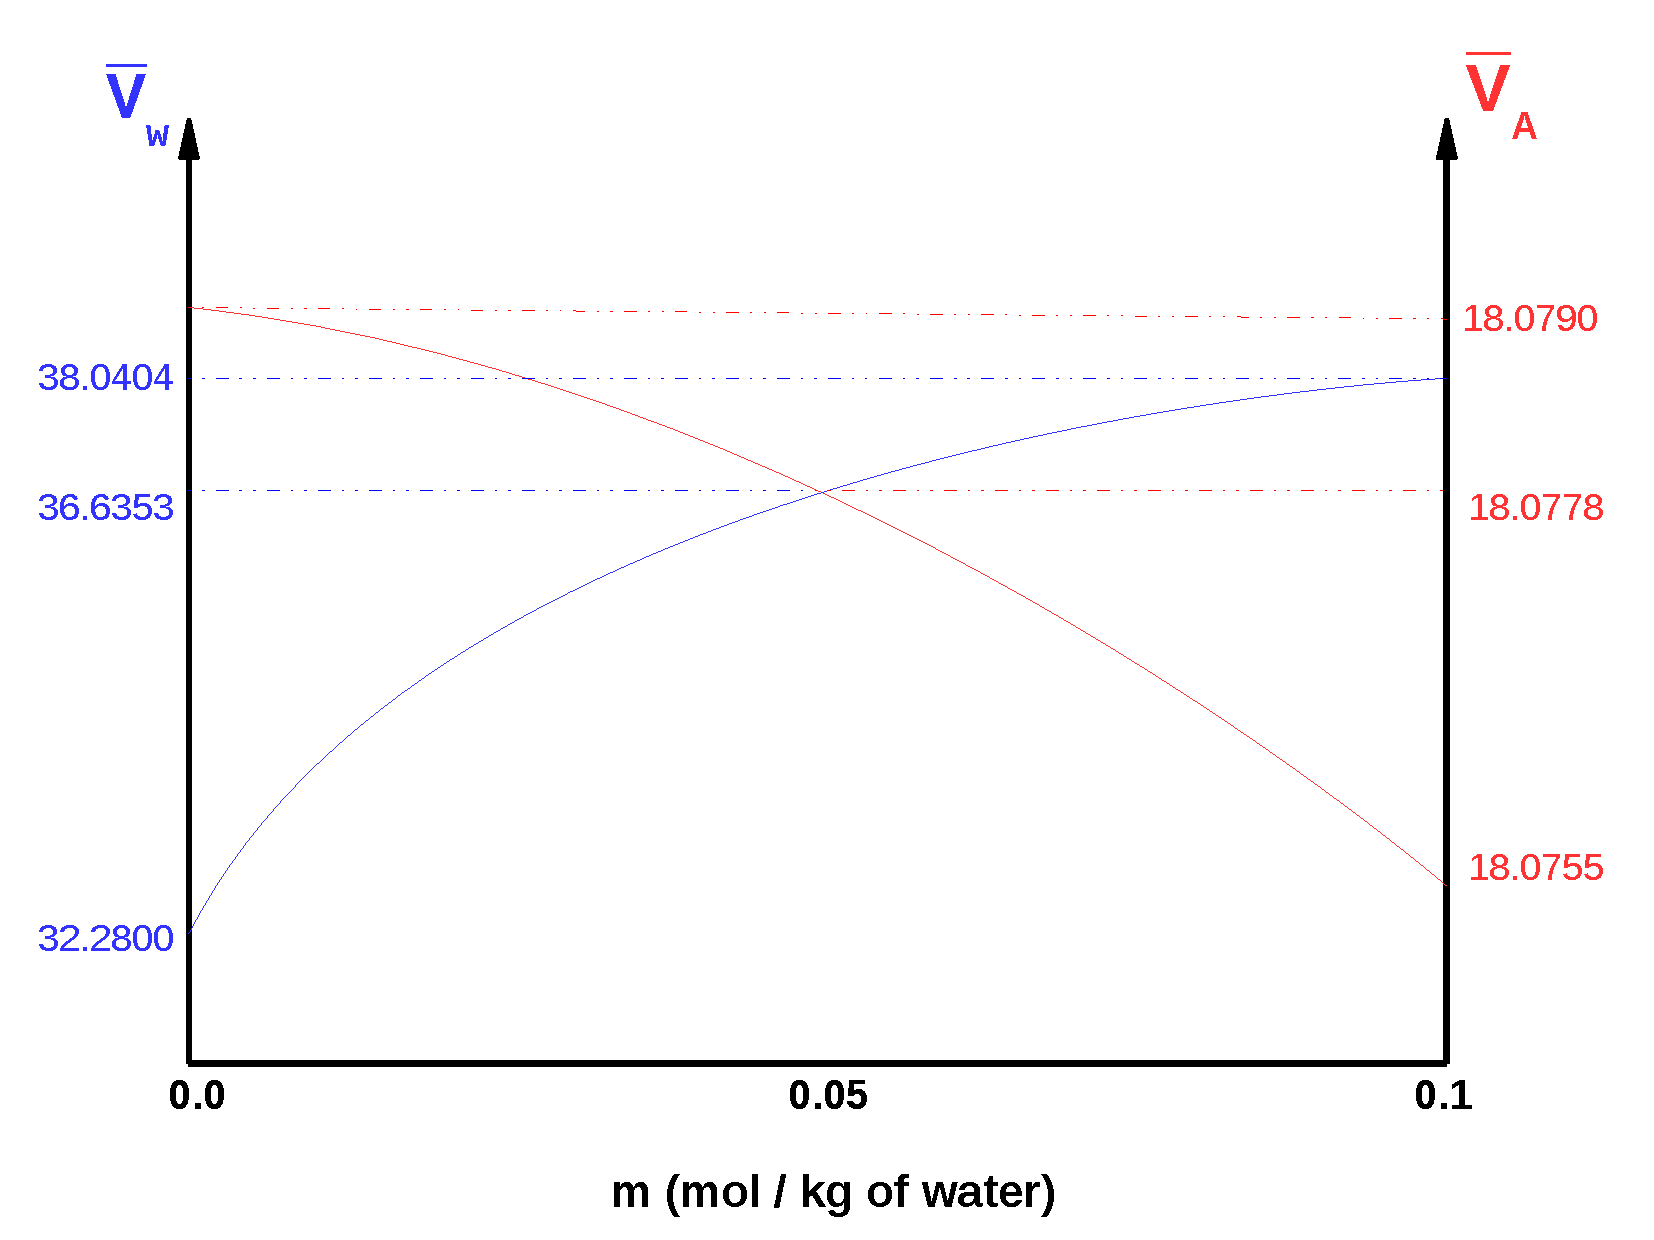
\includegraphics[width=0.75\columnwidth,clip]{./../Pics/Example04_Pic}
          \end{center}
\end{itemize}


\clearpage
            
%%%
%%% EXAMPLE:  NPTEl (Ex 6.3)
%%%
   \item\label{Mod05Ex06} What is the change in entropy when 0.6 m$^{3}$ of CO$_{2}$ and 0.4 m$^{3}$ of N$_{2}$, each at 1 bar and 25 $^{\circ}$C blend to form a gas mixture at the same conditions. Assume ideal gas behaviour and that {\it mole fraction = volume fraction}. 

% SOLUTION
       \noindent{\bf Solution:} For an ideal gas, with the assumption of {\it mole fraction = volume fraction}, \ie $y_{1} = 0.6$ and $y_{2} = 0.4$, with CO$_{2}$:1 and N$_{2}$:2.
      \begin{displaymath}
          \Delta_{\text{mix}}\overline{s}^{\text{igm}} = -R\summation[y_{i}\ln{y_{i}}]{i=1}{2} = 5.5954 \text{ J.(mol.K)}^{-1}
      \end{displaymath}


\clearpage
            
%%%
%%% EXAMPLE:  SM&VN 10.20 (pg 350)
%%%
   \item\label{Mod05Ex07}  For the acetone (Ket) / methanol (MetOH) system, a vapour mixture of $z_{\text{Ket}}$ = 0.25 and $z_{\text{MetOH}}$ = 0.75 is cooled to temperature $T$ in the two-phase region and flows into a separation chamber at a pressure of 1 bar. If the composition of the liquid product is $x_{\text{Ket}}$ = 0.175, calculate $T$  and $y_{\text{Ket}}$. For liquid mixture, assume that
\begin{displaymath}
\ln\gamma_{1} = 0.64x_{2}^{2} \;\;\;\;\;\text{ and }\;\;\;\;\;\ln\gamma_{2}=0.64x_{1}^{2}
\end{displaymath}
For the Antoine equation, 
\begin{displaymath}
\ln P_{i}^{\text{sat}} = A_{i} - \frc{B_{i}}{T + C} \;\;\left(\text{ [P] = kPa and [T] = }^{\circ}\text{C}\right)
\end{displaymath}
$A_{\text{Ket}}$ = 14.3145, $B_{\text{Ket}}$ = 2756.22$^{\circ}$C, $C_{\text{Ket}}$ = 228.060$^{\circ}$C, $A_{\text{MetOH}}$ = 16.5785, $B_{\text{MetOH}}$ = 3638.27$^{\circ}$C, $C_{\text{MetOH}}$ = 239.50$^{\circ}$C.

% SOLUTION
       \noindent{\bf Solution:} This is a typical flash problem for separation of acetone (1) and methanol (2). The feed stream contains 25$\%$-mol of acetone, \ie $z_{1}=0.25$, and after the separation at 1 bar, the resulting liquid stream contains 17.5$\%$-mol, \ie $x_{1}=0.175$. The problem requires temperature of the separation and composition of the gas stream, $y_{i}$. As $\gamma_{i}$ is given, we can consider that the liquid mixture is {\bf not ideal}, therefore the modified Raoult's law can be used,
\begin{displaymath}
    y_{i}P = x_{i}\gamma_{i}P_{i}^{\text{sat}} \;\;\;\longrightarrow y_{1}=\frc{x_{1}\gamma_{1}P_{1}^{\text{sat}}}{P}
\end{displaymath}
    
  \begin{figure}[h]
     \begin{center}
         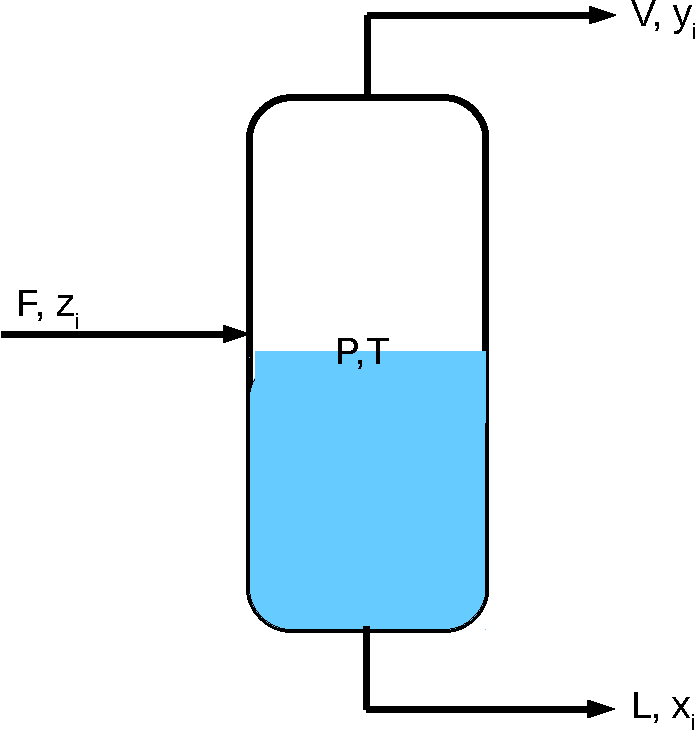
\includegraphics[width=.25\linewidth,clip]{./Figs/FlashDistillation}
     \end{center}
     \caption{Schematic of a flash process, Example~\ref{Mod05Ex07}.}
  \end{figure}

 Using the material balance derived in Section~\ref{Section:04:FlashDistillation},
\begin{eqnarray}
    && Fz_{1} = x_{1}L + y_{1}V\;\;\text{ and for } \;F=1\;\text{ (\ie normalised stream fractions)}\;\;\;\longrightarrow F = L + V = 1,\text{ leading to} \nonumber \\
    && z_{1} = x_{1}L + \frc{x_{1}\gamma_{1}P_{1}^{\text{sat}}}{p}\left(1-L\right)\;(\star)\;\; \text{ with }\;\; P=\summation[P_{i}]{i}{} = y_{1}P + y_{2}P = x_{1}\gamma_{1}P_{1}^{\text{sat}} + x_{2}\gamma_{2}P_{2}^{\text{sat}}\;(\dagger),\nonumber
\end{eqnarray}
therefore, we have 2 equations and 2 unknowns, $L$ and $T$. Let's solve ($\dagger$) first for $T$ with $\gamma_{1}=1.5459$ and $\gamma_{2}=1.0198$
   \begin{displaymath}
       P = x_{1}\gamma_{1}P_{1}^{\text{sat}} + x_{2}\gamma_{2}P_{2}^{\text{sat}} = 100 \text{ kPa} \;\;\;\Rightarrow\;\;\; T = 59.5309\text{ K}
   \end{displaymath}
 With $T$, we can solve ($\star$) for $L$,
   \begin{eqnarray}
       && z_{1} = x_{1}L + \frc{x_{1}\gamma_{1}P_{1}^{\text{sat}}}{p}\left(1-L\right) \nonumber \\
       && L = \frc{z_{1} - \frac{x_{1}\gamma_{1}P_{1}^{\text{sat}}}{P}}{x_{1} - \frac{x_{1}\gamma_{1}P_{1}^{\text{sat}}}{P}} = 0.4306\;\;\rightarrow \;\; V = 0.5694 \nonumber \\
       && y_{1} = \frac{x_{1}\gamma_{1}P_{1}^{\text{sat}}}{P} = 0.3067\;\;\rightarrow \;\; y_{2} = 0.6933\nonumber
   \end{eqnarray}
 



\end{enumerate}


%\part{Fundamental of Chemical Reactions Thermodynamics}
%  \chapter{Chemical Reaction Equilibrium}\label{Chapter:ChemicalReactions}

   \begin{LearningObjectivesBlock}{Learning Objectives}
      Upon completion of this chapter, you will be able to
        \begin{enumerate}
           \item 
        \end{enumerate}
\medskip
     Recommended reading: Chapters 13 of \citet{SmithVanNess_Book}, 8 of \cite{Sandler_Book}, 12 of \citet{Lue_Book}, 14 of \citet{Moran_Book}, 11 of \citet{Devoe_Book} or 7 of \citet{Atkins_Book}.
   \end{LearningObjectivesBlock}


%%%%%%%%%%%%%%%%%%%%%%%%%%%%%%%%%%%%%%%%%%%%%%%%%%%%%%%%%%%%%%%%%
\begin{comment}
   \begin{LearningObjectivesBlock}{Learning Objectives}
      Upon completion of this chapter, you will be able to
        \begin{enumerate}
           \item {\bf Knowledge:} Define, Name, Select, State 
           \item {\bf Comprehension:} Describe, Identify, Discuss
           \item {\bf Application:} Apply, Demonstrate, Employ, Sketch
           \item {\bf Analysis:} Analyse, Compare, Calculate, Solve
           \item {\bf Synthesis:} Determine, Formulate
           \item {\bf Evaluation:} Assess, Check, Estimate, Compare, Measure, Monitor
        \end{enumerate}
\end{comment}
%%%%%%%%%%%%%%%%%%%%%%%%%%%%%%%%%%%%%%%%%%%%%%%%%%%%%%%%%%%%%%%%%

%%%% ETOC
\localtableofcontents
   
%%% SECTION
\section{Introduction}\label{Chapter:ChemicalReactions:Section:Introduction}
In previous Chapters, we studied the thermodynamic behaviour of gases and liquids at equilibrium conditions assuming that species do not react. However, in many industrial, environmental and bio-medical applications, chemical reactions are the driving force behind important processes.
      \begin{wrapfigure}{r}{0.5\textwidth}%{figure}[hpt]
         \begin{center}
           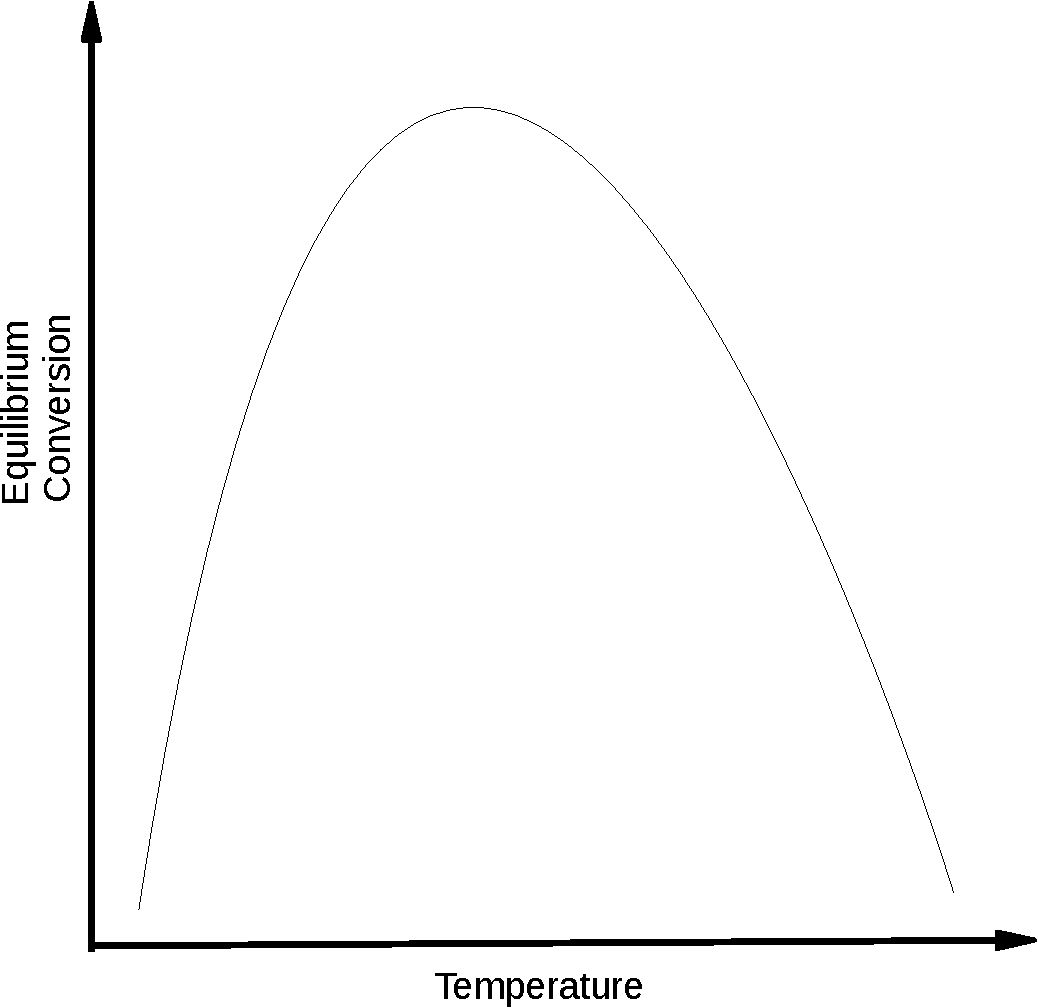
\includegraphics[width=0.5\columnwidth,clip]{./Figs/Mod06_SchematicEqReaction_Temp_b}
           \caption{Sketch of equilibrium reaction and temperature.}\label{Mod06Fig01}
         \end{center}
       \end{wrapfigure}%{figure}
      Reactive systems are often characterised in terms of the maximum possible yield of the target product(s) at prescribed conditions, starting from the reactants (\ie raw materials). From {\it chemical kinetics} theory, rates of reaction and the reaction mechanisms\footnote{Here, it is important to define two terms commonly used in chemical kinetics theory:
        \begin{enumerate}[a)]
           \item {\it rate of reaction}: changes in the reactants concentrations with time, $\mfr[C]{}{\text{react}}=\mfr[C]{}{\text{react}}(t)$ (\ie `speed' of the reaction) and,
           \item {\it mechanisms of reactions}: stages of the reaction (in molecular level) that leads to the consumption of reactants and intermediate products, and production of final and intermediate products.
        \end{enumerate}
         }
        are often strongly influenced by temperature and pressure conditions. In several cases, reaction rates rise as temperature increases and in reactions involving gaseous phases, increasing of pressure may also lead to `faster' reactive conversions. In fact, reaction data from several applications (from combustion and geochemistry to biochemistry) show that conversion rates from reactants to products do not increase {\it monotonically}, but rather reach a {\it maximum} of conversion and smoothly decrease as schematically shown in Fig.~\ref{Mod06Fig01}.

Consider a chemical reaction in the gaseous phase,
     \reaction[chemreaction:reaction1]{A (g) + B (g) <=> C (g) + D (g)}

\noindent where initially $\left(\text{\ie at time } t_{0}=0\right)$ there are 1 mol of reactants $A$ and $B$ (each) in a {\it closed system}. Molecules of $A$ and $B$ are in continuous and random movement and collide with each other forming products $C$ and $D$. At this stage, the consumption/depletion of molecules of $A$ and $B$ dominates the dynamics in the system. However, as the reaction progresses $\left(\text{\ie at } t > t_{0}\right)$, the amount of molecules (\ie number of moles) of $C$ and $D$ increases and these species become dominant in the system. Collisions between $A$ and $B$ may still occur, but as they are no longer abundant, conversion from reactants to products get smaller, however molecules of $C$ and $D$ (both also in gaseous form) also collide and may produce $A$ and $B$. 

Thus, while initially the {\it forward} reaction dominates $\left(\text{\ie } A (g) + B (g) \rightarrow C (g) + D (g)\right)$, as reaction progress the {\it backward} reaction $\left(\text{\ie } A (g) + B (g) \leftarrow C (g) + D (g)\right)$ becomes increasingly relevant, which eventually leads to two reaction rates of equal value. After this stage, the concentration of all species in the system is invariant (\ie constant) with no tendency to change except if a perturbation is imposed to the system (\eg addition/removal of heat, increase/decrease of pressure, addition/removal of species etc). At such conditions, the reaction is said to be in {\it equilibrium}. The aim of the study of {\it chemical kinetics} is to investigate the mechanisms that leads to optimal reactions (\ie `faster' and with larger conversion ratio), whereas \blue{reaction thermodynamics} investigates the conditions at {\it equilibrium}.\index{Chemical kinetics}\index{Chemical reaction!Equilibrium}

In the application of {\it chemical reaction equilibrium} to problems relevant to industry, the aim is to ensure {\it maximum} conversion at prescribed pressure and temperature conditions. Reactions for which the conversion is (approximately) 100$\%$ are often referred as \blue{\it irreversible}, whereas reactions that have lower conversion rates are called \blue{\it reversible}.

\medskip
Chemical reactions that occur in a single phase (either solid, liquid or gas) are called \blue{\it homogeneous}, \eg\index{Chemical reaction!Reversible}\index{Chemical reaction!Irreversible}
\begin{enumerate}[a)]
  \item formation of NO$_{\text{x}} \left(\text{NO and NO}_{2}\right)$ in atmospheric pollution:
    \begin{displaymath}
      \begin{cases}
         N_{2} (g) + O_{2} (g) &\Longleftrightarrow 2 NO (g),  \\
         \frac{1}{2} N_{2} (g) + O_{2} (g) &\Longleftrightarrow NO_{2} (g),  \\
      \end{cases}
    \end{displaymath}
 \item {\it Fischer esterification} reaction of ethanol and acetic acid to produce ethyl acetate:
        \begin{displaymath}
           CH_{3}CH_{2}OH (l) + CH_{3}COOH (l) \Longleftrightarrow CH_{3}COOCH_{2}CH_{3} (l),
        \end{displaymath}
\end{enumerate}

Reactions that progress at different phases are called \blue{\it heterogeneous}, \eg
\begin{enumerate}[a)]
    \item strong acid-alkali reactions:
    \begin{displaymath}
      \begin{cases}
           H_{2}SO_{4} (\text{aq.}) + 2 NaOH (\text{aq.}) \Longleftrightarrow&  Na_{2}SO_{4} (s) + H_{2}O (l) \\
           HCl (\text{aq.}) + KOH (\text{aq.}) \Longleftrightarrow& KCl (s) + H_{2}O (l),  \\
           2 HCl (\text{aq.}) + Mg(OH)_{2} (s)  \Longleftrightarrow& MgCl_{2} (s) + 2 H_{2}O (l), \\
      \end{cases}
    \end{displaymath}
    \item combustion of natural gas:
        \begin{displaymath}
           CH_{4} (g) + O_{2} (g) \Longleftrightarrow CO_{2} (g) + H_{2}O (l),
        \end{displaymath}
    \item reduction of solid oxides:
        \begin{displaymath}
           NiO (s) + H_{2} (g) \Longleftrightarrow Ni (s) + H_{2}O (l). 
        \end{displaymath}        
\end{enumerate}

Reaction conditions are, thus, critical to achieve the maximum possible conversion rate. The main aim of this chapter is to study the thermodynamic relations necessary to predict equilibrium conversion of {\it homogeneous chemical reactions}. 

%%% SECTION
\section{Reaction Coordinate}\label{Chapter:ChemicalReactions:Section:ReactionCoordinate}\index{Chemical reaction!Coordinate}\index{Reaction coodinate|see{Chemical reaction}}
\begin{subequations}
    For a chemical reaction in general form:
        \reaction[chemreaction:reaction]{\nu_{1} A_{1} + \nu_{2} A_{2}  + ... \nu_{k} A_{k} <=> \nu_{l} A_{l} + \nu_{m} A_{m} + ... + \nu_{\mathcal{C}} A_{\mathcal{C}} }
    where $\nu_{i}$ is the \blue{\it molar stoichiometric coefficient}, $A_{i}$ are chemical species and $\mathcal{C}$ is the total number of species in the system. For convention, \underline{positive $\nu_{i}$ stands for products} whereas \underline{negative $\nu_{i}$ is for reactants}, and the reaction can be expressed as an algebraic equation,\index{Chemical reaction!Stoichiometric coefficient}\index{Stoichiometric coefficient|see{Chemical reaction}}
    \begin{displaymath}
       \nu_{l} A_{l} + \nu_{m} A_{m} + ... + \nu_{\mathcal{C}} A_{\mathcal{C}} - \left(\nu_{1} A_{1} + \nu_{2} A_{2}  + ... \nu_{k} A_{k}\right) = 0,
    \end{displaymath}
    or simply
    \begin{equation}
      \summation[\nu_{i}A_{i}]{i=1}{\mathcal{C}} = 0.\label{Chapter:ChemicalReactions:Eqn:2}
    \end{equation}
\bigskip

    Let's consider, for example, the reaction for production of synthesis gas (or syngas, a mixture of hydrogen and carbon monoxide) from natural gas, 
        \reaction[chemreaction:syngas]{ CH_{4} + H_{2}O <=> CO + 3 H_{2} }
    the molar stoichiometric coefficients are $\nu_{CH_{4}}=\nu_{H_{2}O}=-1$, $\nu_{CO}=1$ and $\nu_{H_{2}}=3$, and the reaction can be written in equation form as,
    \begin{displaymath}
       CO + 3 H_{2} - CH_{4} - H_{2}O = 0.
    \end{displaymath}
    This {\it steam reforming reaction} indicates that as CH$_{4}$ is consumed (along with the water), CO and H$_{2}$ are produced. More specifically, if initially there are 1 mol of CH$_{4}$, 1 mol of H$_{2}$O, 0 mol of CO and 0 mol of H$_{2}$,
     \begin{center}
        \begin{tabular}{ l | c c c c c c c}
                           & CH$_{4}$  & + & H$_{2}$O & $\Longleftrightarrow$ &  CO & + & 3 H$_{2}$ \\
                 $t = 0 $  &   1      &   &    1     &                       &  0 &    &   0      \\
              $t = t_{i} $  &   X      &   &    X     &                       &  X &    &   3X      \\
        \hline
                           &  1-X     &   &  1-X     &                       &   X  &    & 3X
     \end{tabular}
    \end{center}
    Thus, as reaction progress $X$ moles of CH$_{4}$ and H$_{2}$O are consumed whereas $X$ and $3X$ moles of CO and H$_{2}$, respectively, are formed. As the reaction needs to be stoichiometrically balanced,
    \begin{displaymath}
       \frc{d n_{CH_{4}}}{\nu_{CH_{4}}} = \frc{d n_{H_{2}O}}{\nu_{H_{2}O}} = \frc{d n_{CO}}{\nu_{CO}} = \frc{d n_{H_{2}}}{\nu_{H_{2}}},
    \end{displaymath}
    where $n_{i}$ is the number of moles of species $i$. This relation can be generalised for {\it any} chemical reaction as,
    \begin{displaymath}
       \frc{d n_{1}}{\nu_{1}} = \frc{d n_{2}}{\nu_{2}} = \cdots = \frc{d n_{\mathcal{C}}}{\nu_{\mathcal{C}}}.
    \end{displaymath}
    \begin{shaded}
       These equalities lead to the definition of \underline{reaction coordinate}, \blue{$\varepsilon$}, the {\it extension in which a reaction has progressed},
       \begin{equation}
          \frc{d n_{1}}{\nu_{1}} = \frc{d n_{2}}{\nu_{2}} = \cdots = \frc{d n_{\mathcal{C}}}{\nu_{\mathcal{C}}} = d\varepsilon.\label{Chapter:ChemicalReactions:Eqn:2a}
       \end{equation}
       Assuming  that at $t=t_{0}=0$ the initial composition is $n_{i} = n_{i,0}$ and the reaction has not started yet, \ie $\varepsilon=0$. Integrating Eqn.~\ref{Chapter:ChemicalReactions:Eqn:2a} from $t_{0}$ to $t_{i}$,
       \begin{eqnarray}
           && \int\limits_{n_{i,0}}^{n_{i}} dn_{i} = \nu_{i}\int\limits_{0}^{\varepsilon}d\varepsilon \nonumber \\
           && n_{i} = n_{i,0} + \nu_{i}\varepsilon,\;\;\;\;\forall i=\left\{1,2,\cdots,\mathcal{C}\right\}\label{Chapter:ChemicalReactions:Eqn:2b}
       \end{eqnarray}
       For a total number of moles $n$, 
       \begin{equation}
            n = \summation[n_{i}]{i=1}{\mathcal{C}} = \summation[n_{i,0}]{i=1}{\mathcal{C}} + \varepsilon \summation[\nu_{i}]{i=1}{\mathcal{C}},\label{Chapter:ChemicalReactions:Eqn:2c}
       \end{equation}
       or in compressed notation format,
       \begin{equation}
          n = n_{0} + \nu\varepsilon,\label{Chapter:ChemicalReactions:Eqn:2d}
       \end{equation}
       where $n_{0}=\summation[n_{i,0}]{}{}$, $\nu=\summation[\nu_{i}]{}{}$ and $n=\summation[n_{i}]{}{}$. Now, we can define the composition (as mole fraction) of species $i$,
       \begin{equation}
          y_{i} = \frc{n_{i}}{n} = \frc{n_{i,0} + \nu_{i}\varepsilon}{n_{0} + \nu\varepsilon}.\label{Chapter:ChemicalReactions:Eqn:2e}
       \end{equation}
       \blue{For an \underline{inert species} $k$, \ie chemical compound that does not react but is present in the reactive system, $\nu_{k}=0$.} 
    \end{shaded}

    From the initial steam reforming reaction example, let's assume that initially there are 2 moles of CH$_{4}$, 1 mol of H$_{2}$O, 1 mol of CO and 4 moles of H$_{2}$ in a closed system. Thus, the initial number of moles, $n_{0}=\summation[n_{i,0}]{}{} = 2+1+1+4 = 8$. Note that before the reaction starts there are already products in the system. The overall molar stoichiometric coefficient is
    \begin{displaymath}
         \nu = \summation[\nu_{i}]{}{} = -1 -1 + 1+ 3 = 2.
    \end{displaymath}
    The gaseous composition is expressed by Eqn.~\ref{Chapter:ChemicalReactions:Eqn:2e},
    \begin{displaymath}
          y_{i} = \frc{n_{i,0} + \nu_{i}\varepsilon}{n_{0} + \nu\varepsilon}
          \begin{cases}
               y_{CH_{4}} = \frc{2-\varepsilon}{8+2\varepsilon},\;\;\; y_{H_{2}O} = \frc{1-\varepsilon}{8+2\varepsilon} \\
               y_{CO} = \frc{1 + \varepsilon}{8+2\varepsilon},\;\;\; y_{H_{2}} = \frc{4+\varepsilon}{8+2\varepsilon} \\
          \end{cases}
    \end{displaymath}

\bigskip

Given the set of 3 reactions below for the formation of CO and CO$_{2}$,
          \reaction[chemreaction:FormationCO2]{ C + O_{2} <=> CO_{2}}
          \reaction[chemreaction:FormationCO]{2C + O_{2} <=> 2CO } 
          \reaction[chemreaction:FormationCOCO2]{2CO + O_{2} <=> 2CO_{2}}
    It is easy to notice that, \ref{chemreaction:FormationCO} + \ref{chemreaction:FormationCOCO2} = \ref{chemreaction:FormationCO2}. In matricial form (adopting the stoichiometric notation),
    \begin{center}
      \begin{tabular}{ c | c c c c }
                                          & C   & O$_{2}$ & CO & CO$_{2}$ \\
\hline
       \ref{chemreaction:FormationCO2}    & -1  & -1     & 0   &   1 \\
       \ref{chemreaction:FormationCO}     & -2  & -1     & 2   &   0 \\
       \ref{chemreaction:FormationCOCO2} & 0   & -1     & -2  &   2 
      \end{tabular}
    \end{center}
    Row 1 (\ref{chemreaction:FormationCO2}) is a linear combination of rows 2 and 3 (\ie Row 1 = 0.5 $\times$ Row 2 + 0.5 $\times$ Row 3). This indicates that 2 out of the 3 rows of the matrix are {\it linearly independent} and one of them is {\it linearly dependent}, \ie it can be written as a linear combination of the other two rows. Such linear algebra fundamental concept, linear independency\footnote{A finite set $\mathcal{S}=\left\{\mathbf{x_{1}}, \mathbf{x_{2}}, \cdots, \mathbf{x_{m}}\right\}$ of vectors in $\mathbb{R}^{n}$ space is said to be {\bf linearly dependent} if there exist scalars (\ie real numbers), $\alpha_{1}, \alpha_{2}, \cdots, \alpha_{m}$ (not all of them equal to zero), such that
    \begin{displaymath}
       \alpha_{1}\mathbf{x_{1}} + \alpha_{2}\mathbf{x_{2}} + \cdots + \alpha_{m}\mathbf{x_{m}} = 0.
    \end{displaymath}
    If a set of vectors is said to be linearly dependent, then at least one vector can be expressed as a {\it linear combination} of the others. A good review of linear dependence in vector space can be found in \href{http://linear.ups.edu/html/section-LI.html}{http://linear.ups.edu/html/section-LI.html}.} in vector space, is extended to define independent chemical reactions, \ie the smallest set of reactions that, when linearly combined results in {\it all possible chemical reactions} among the species present in the system. 

    In the following set of reactions,
          \reaction[chemreaction:O2]{ 2 O <=> O_{2}} 
          \reaction[chemreaction:FormationCO-b]{ C + O <=> CO }
          \reaction[chemreaction:FormationCO2-b]{C + 2O <=> CO_{2}}
    none of them can be expressed as a linear combination of the remaining reactions. These are, thus, {\it independent reactions}, and several chemical reactions can be written as combinations of this set. Combining these reactions to eliminate reaction~\ref{chemreaction:O2} (fusion of atomic oxygen),
          \begin{displaymath}
             \text{Independent reactions:}
                \begin{cases}
                   2 C + O_{2} \Longleftrightarrow 2 CO \;\;\;\;\; (2\ref{chemreaction:FormationCO-b} - \ref{chemreaction:O2}) \\
                   C + O_{2} \Longleftrightarrow CO_{2} \;\;\;\;\;\;\; (\ref{chemreaction:FormationCO2-b}-\ref{chemreaction:O2})
                \end{cases}
          \end{displaymath}
    provide a reduction of the order of the system (from three reactions/equations to just 2 independent reactions/equations). Other sets of 2 reactions can be readily obtained from linear combinations of reactions~\ref{chemreaction:O2}-~\ref{chemreaction:FormationCO2-b}, \eg
          \begin{displaymath}
             \text{Independent reactions:}
             \begin{cases}
                CO_{2} \Longleftrightarrow CO + O \;\;\;\; (\ref{chemreaction:FormationCO-b}-\ref{chemreaction:FormationCO2-b}) \\
                2O  \Longleftrightarrow O_{2},
             \end{cases}
          \end{displaymath}
    These reactions results in single reaction: 
          \reaction[chemreaction:CO2-CO-O2]{2CO_{2} <=>  2CO + O_{2}}
    \begin{shaded}
       \noindent Thus, for a set of \underline{independent chemical reactions}, Eqn.~\ref{Chapter:ChemicalReactions:Eqn:2b} can be rewritten as,
          \begin{equation}
             n_{i} = n_{i,0} + \summation[\nu_{ij}\varepsilon_{j}]{j}{},\label{Chapter:ChemicalReactions:Eqn:2f}
          \end{equation}
       where $i$ refers to chemical species, whereas $j$ refers to reactions,
          \begin{displaymath}
             n = \summation[n_{i,0}]{i}{} + \summation[\summation[\nu_{ij}\varepsilon_{j}]{i}{}]{j}{} = n_{0} + \summation[\left(\summation[\nu_{ij}]{j}{}\right)\varepsilon_{j}]{i}{},
          \end{displaymath}
       For simplicity of notation, let's use $\nu_{j}=\summation[\nu_{ij}]{i}{}$, thus
          \begin{equation}
             n = n_{0} + \summation[\nu_{j}\varepsilon_{j}]{j}{}.\label{Chapter:ChemicalReactions:Eqn:2g}
          \end{equation}
       Now, for composition of species $i$ in multiple reactions $j$,
       \begin{equation}
          y_{i} = \frc{n_{i}}{n} = \frc{n_{i,0} + \summation[\nu_{ij}\varepsilon_{j}]{j=1}{\mathcal{R}}}{n_{0} + \summation[\nu_{j}\varepsilon_{j}]{j=1}{\mathcal{R}}},\label{Chapter:ChemicalReactions:Eqn:2h}
       \end{equation}
       where $\mathcal{R}$ is the number of independent chemical reactions.
    \end{shaded}

\bigskip

    As an example, let's consider the steam reforming reactions,
          \begin{displaymath}
              \begin{cases}
                  CH_{4} + H_{2}O \Longleftrightarrow CO + 3 H_{2}, \\
                  CH_{4} + 2H_{2}O \Longleftrightarrow CO_{2} + 4 H_{2}.
              \end{cases}
          \end{displaymath}
    Consider that at $t=0$, there are 2 moles of methane and 3 moles of water in the system $\left(\text{\ie } n_{0}=5\right)$. Let's obtain expressions for the gaseous compositions. As a initial step, a table with species ($i$) and reactions ($j$) may be expressed as,
    \begin{center}
       \begin{tabular}{ c | c c c c c | c} 
          $(i=)$  & CH$_{4}$ & H$_{2}$O & CO & CO$_{2}$ & H$_{2}$ &  \\
\hline
            $j$   &         &         &     &         &        & $\nu_{j}$ \\
\hline
             1    &   -1    &    -1   &   1 &    0    &   3    &    2 \\
             2    &   -1    &    -2   &   0 &    1    &   4    &    2 \\
       \end{tabular}
    \end{center}
    therefore,
      \begin{displaymath}
         n = n_{0} + \summation[\nu_{j}\varepsilon_{j}]{j}{} = 5 + 2\varepsilon_{1} + 2\varepsilon_{2},
      \end{displaymath}
    and compositions are (from Eqn.~\ref{Chapter:ChemicalReactions:Eqn:2h}),
    \begin{displaymath}
        \begin{cases}
            y_{CH_{4}} = \frc{2 - \varepsilon_{1} - \varepsilon_{2}}{5 + 2\varepsilon_{1} + 2\varepsilon_{2}},\;\;\; y_{H_{2}O} = \frc{3 - \varepsilon_{1} - 2\varepsilon_{2}}{5 + 2\varepsilon_{1} + 2\varepsilon_{2}}, \\
            y_{CO}   = \frc{\varepsilon_{1}}{5 + 2\varepsilon_{1} + 2\varepsilon_{2}},\;\;\; y_{CO_{2}} = \frc{\varepsilon_{2}}{5 + 2\varepsilon_{1} + 2\varepsilon_{2}} \;\;\text{ and }\;\;\;y_{H_{2}} = \frc{3\varepsilon_{1}+4\varepsilon_{2}}{5 + 2\varepsilon_{1} + 2\varepsilon_{2}}  \\
        \end{cases}
    \end{displaymath}

\end{subequations}

%%% SECTION
\section{Standard Enthalpy of Reaction}\label{Chapter:ChemicalReactions:Section:EnthalpyGibbsReaction}\index{Enthalpy! of reaction}\index{Enthalpy! of combustion}\index{Enthalpy! of formation}\index{Standard enthalpy of formation|see{Enthalpy}}\index{Standard enthalpy of reaction|see{Enthalpy}}\index{Standard enthalpy of combustion|see{Enthalpy}}
\begin{subequations}
   Given a general homogeneous chemical reaction,
     \reaction[chemreaction:simplehomogeneousreaction]{\nu_{A}A + \nu_{B}B <=> \nu_{C}C + \nu_{D}D}
   the {\it standard enthalpy of reaction}, $\Delta H^{\circ}_{\text{r}}$ is the heat associated with a chemical reaction that occurs at constant temperature $T$ and at {\it standard pressure} $P$ of 101.325 kPa (\ie 1 atm). In other words, it is the change in enthalpy that occurs when $\nu_{A}$ moles of $A$ and $\nu_{B}$ moles of $B$ at standard state and temperature $T$ are fully converted into $\nu_{C}$ moles of $C$ and $\nu_{D}$ moles of $D$ at standard states and at the same temperature $T$. {\it Standard states} commonly used are:
   \begin{enumerate}[a)]
       \item Gases: pure substance in the ideal gas state at 1 atm;
       \item Liquids and solids: pure liquid or solid at 1 atm.
   \end{enumerate}
   In the literature, data on standard enthalpy of reaction is typically reported at 25$^{\circ}$C. Using the sign convention for molar stoichiometric coefficient, the standard enthalpy of reaction is
   \begin{equation}
      \Delta H^{\circ}_{\text{r}} = \summation[\nu_{i}\Delta H^{\circ}_{i,f}]{i}{},\label{Chapter:ChemicalReactions:Eqn:3a}
   \end{equation}
   \begin{table}
     \begin{center}
       \begin{tabular}{l c | l l}
         \hline
         {\bf Species}        &                    &  $\Delta H^{\circ}_{f}$               &    $\Delta H^{\circ}_{c}$              \\
                              &                    &  $\left(\text{kJ.mol}^{-1}\right)$  & $\left(\text{kJ.mol}^{-1}\right)$     \\
         \hline
         Benzene              & C$_{6}$H$_{6}$ (l)  &  49.0                               &-3268.0                               \\
         Ethane               & C$_{2}$H$_{6}$ (g)  &  -84.7                              & -1560.0                              \\
         Methane              & CH$_{4}$ (g)       &  -74.8                              & -890.0                               \\
         Glucose              & C$_{6}$H$_{12}$O$_{6}$ (s)&  -1274.0                       & -2801.0                               \\
         Methanol             & CH$_{3}$OH (l)     &  -238.7                             & -721.0                               \\
         Carbon dioxide       & CO$_{2}$ (l)       &  -393.52                            &  --                                 \\
         \hline
       \end{tabular}
       \caption{Standard enthalpies of formation and combustion of organic compounds at 298.15 K \citep[extracted from][]{Atkins_Book}.}\label{Chapter:ChemicalReactions:Table:EnthalpyFormation}
     \end{center}
   \end{table}
   where $\Delta H^{\circ}_{i,f}$ is the {\it standard enthalpy of formation}, \ie the standard enthalpy of a reaction in which {\it one mol of a given substance is formed from elements}. The elements are assumed to react at the most stable phase at a given temperature and standard pressure conditions. For example, the standard enthalpy of formation of liquid benzene at 25$^{\circ}$C (Table~\ref{Chapter:ChemicalReactions:Table:EnthalpyFormation}) refers to the reaction\footnote{Thermo-physical properties of a number of chemical species can be found in the \href{http://webbook.nist.gov/chemistry/}{NIST Chemistry WebBook}.},
   \begin{displaymath}
     6 C\text{ (s, graphite)} + 3 H_{2}\text{ (g)} \Longleftrightarrow C_{6}H_{6}\text{ (l)},\;\;\;\;\;\;\Delta H^{\circ}_{f}=49.0\text{ kJ.mol}^{-1}
   \end{displaymath}
   Data basis of the {\it standard enthalpy of formation} for common chemical species can be found in any chemical engineering handbook and on thermodynamic textbooks. Some {\it standard reaction enthalpies} have special names due to the practical relevances. For example, the {\it standard enthalpy of combustion}, $\Delta H^{\circ}_{c}$, is the standard reaction enthalpy for complete oxidation of an organic chemical species to gaseous CO$_{2}$ and liquid H$_{2}$O $\left(\text{and gaseous N}_{2}\text{ if N is present in the oxidised species}\right)$, \eg for the combustion of glucose,
   \begin{displaymath}
     C_{6}H_{12}O_{6}\text{ (s)} + 6 O_{2} \text{ (g)} \Longleftrightarrow 6 CO_{2}\text{ (g)} + 6 H_{2}O\text{ (l)},
   \end{displaymath}
   the calculated standard enthalpy of combustion ( Eqn.~\ref{Chapter:ChemicalReactions:Eqn:3a}) is
   \begin{displaymath}
      \Delta H^{\circ}_{\text{gluc},c} = 6 \Delta H^{\circ}_{CO_{2}, f} + 6 \Delta H^{\circ}_{H_{2}O, f} - \left(6\cancelto{0}{\Delta H^{\circ}_{O_{2}, f}} + \Delta H^{\circ}_{\text{gluc},  f} \right) = -2802.10\text{ kJ.mol}^{-1},
   \end{displaymath}
   which slightly over-predict the tabulated value (Table~\ref{Chapter:ChemicalReactions:Table:EnthalpyFormation}).
   In a similar way, Eqn.~\ref{Chapter:ChemicalReactions:Eqn:3a} can be extended to all thermodynamic potentials, $M=\left\{U, H, A, G, S\right\}$, as
   \begin{equation}
      \Delta M^{\circ}_{\text{r}} = \summation[\nu_{i}\Delta M^{\circ}_{i,f}]{i}{}.\label{Chapter:ChemicalReactions:Eqn:3b}
   \end{equation}
  
\end{subequations}

%%% SECTION
\section{Criteria for Chemical Reaction Equilibrium}\label{Chapter:ChemicalReactions:Section:CriteriaEquibrium}\index{Gibbs free energy!Partial molar}
\begin{subequations}

   For simplicity of the analysis, let's assume {\it single homogeneous chemical reactions}. The total Gibbs free energy of a system is obtained from
     \begin{equation}
         G^{t} = \summation[n_{i}\overline{G}_{i}]{i=1}{\mathcal{C}} = \summation[\left(n_{i,0}+\nu_{i}\varepsilon\right)\overline{G}_{i}]{i=1}{\mathcal{C}}\label{Chapter:ChemicalReactions:Eqn:4a}
     \end{equation}
   where $\overline{G}_{i}$ is the partial molar Gibbs free energy. At equilibrium (Fig.~\ref{Chapter:ChemicalReactions:Fig:Fig02}), $\left(dG^{t}\right)_{T,P} = 0$, \ie
       \begin{eqnarray}
          && dG^{t} = d(n\overline{G}) = nd\overline{G} + \overline{G}dn \;\;\;\; \blue{\times \frc{1}{d\varepsilon}} \nonumber \\
          && \frc{dG^{t}}{d\varepsilon} = n\frc{d\overline{G}}{d\varepsilon} + \overline{G}\frc{dn}{d\varepsilon} = 0 \nonumber \\
          && \text{in a closed system, } dn = 0 \Longrightarrow \frc{dG^{t}}{d\varepsilon} = \frc{d\overline{G}}{d\varepsilon} = 0\;\;\text{ (equilibrium criteria).} \nonumber
       \end{eqnarray}
      \begin{figure}[hpt]
         \begin{center}
           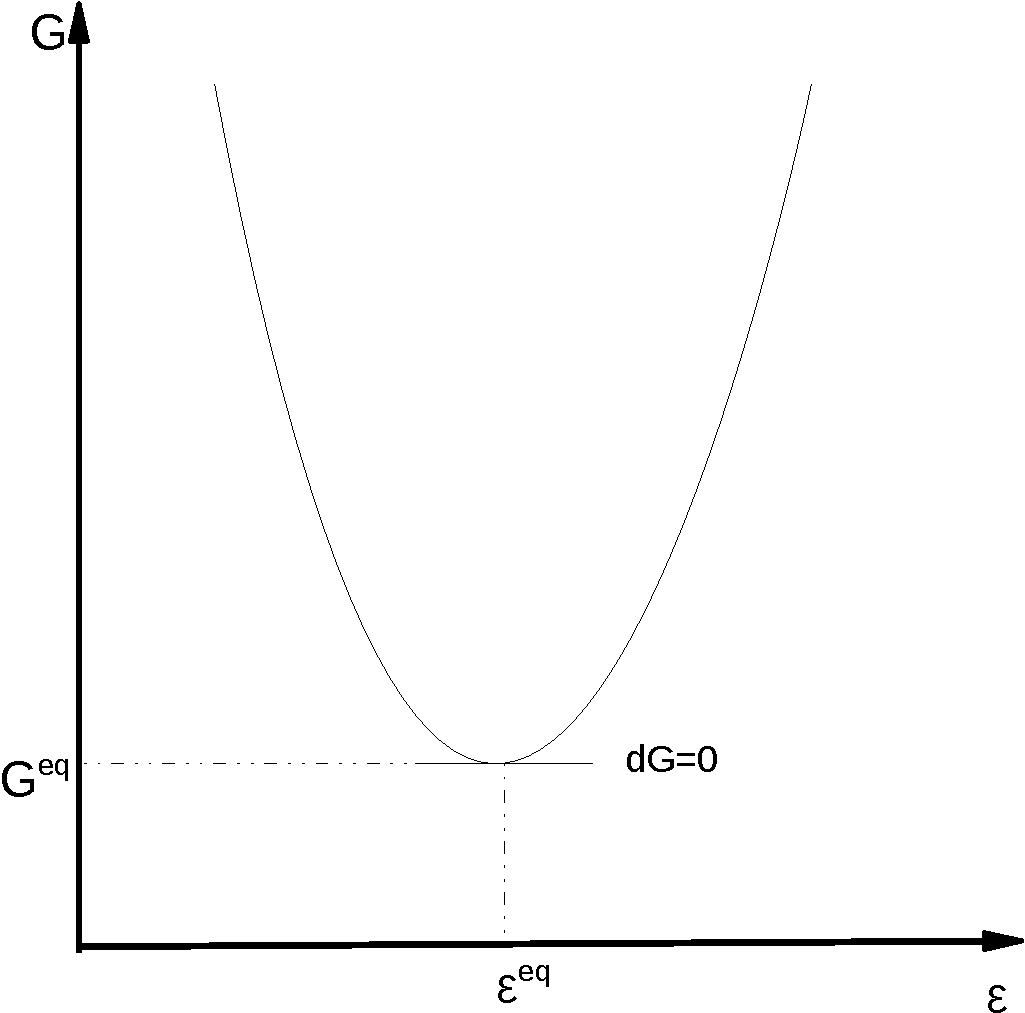
\includegraphics[width=0.5\columnwidth,clip]{./Figs/Mod06_SchematicEquilibriumGibbs_b}
           \caption{Sketch of equilibrium Gibbs free energy.}\label{Chapter:ChemicalReactions:Fig:Fig02}
         \end{center}
      \end{figure} 
   Differentiating Eqn.~\ref{Chapter:ChemicalReactions:Eqn:4a} \wrt $\varepsilon$,
       \begin{displaymath}
           \frc{dG^{t}}{d\varepsilon} = \cancelto{0}{\frc{d}{d\varepsilon}\summation[n_{i,0}\overline{G}_{i}]{i}{}} + \frc{d}{d\varepsilon}\left[\summation[\left(\nu_{i}\varepsilon\right)\overline{G}_{i}]{i}{}\right] = 0,
       \end{displaymath}
   where the summation in brackets can be simplified as,
       \begin{displaymath}
           \frc{d}{d\varepsilon}\left(\nu_{i}\varepsilon \overline{G}_{i}\right) = \nu_{i}G_{i}\cancelto{1}{\frc{d\varepsilon}{d\varepsilon}} + \nu_{i}\varepsilon\cancelto{0}{\frc{d \overline{G}_{i}}{d\varepsilon}} = \nu_{i}\overline{G}_{i}
       \end{displaymath} 
   with $\nu_{i}$ constant, leading to
        \begin{shaded}
          \begin{equation}
             \summation[\nu_{i}\overline{G}_{i}]{i}{} = 0 = \summation[\nu_{i}\mu_{i}]{i}{}.\label{Chapter:ChemicalReactions:Eqn:4b}
          \end{equation}
        \end{shaded}
\end{subequations}


%%% SECTION
\section{Equilibrium Constant of Reactions}\label{Chapter:ChemicalReactions:Section:EquilibriumConstantReactions}\index{Chemical reaction!Equilibrium constant}\index{Equilibrium constant|see{Chemical reaction}}
\begin{subequations}

   The chemical potential was previously defined for mixtures (see Eqn.~\ref{Chapter:SolutionThermodynamics:Eqn:fugacity1b}) as,
       \begin{displaymath}
           \mu_{i} = \Partial[\left(nG\right)]{n_{i}}{T,P,n_{j\ne i}} = \overline{G}_{i} = RT\ln{\overline{f}_{i}} + C_{i}(T),
       \end{displaymath}
   where $\overline{f}_{i}$ is the fugacity of component $i$ in the mixture\footnote{In Chapter~\ref{Chapter:SolutionThermodynamics}, we have studied forms to calculate $\mfr[\overline{f}]{i}{j}$:
      \begin{enumerate}[a)]
          \item ideal gases: $\mfr[\overline{f}]{i}{\text{ig}} =  y_{i}P=P_{i}$ (Dalton law);
          \item real gases: $\mfr[\overline{\phi}]{i}{V}  = \frc{\mfr[\overline{f}]{i}{V}}{y_{i}P}$;
          \item ideal solution: $\mfr[\overline{f}]{i}{\text{id}} = x_{i}\mfr[f]{i}{L}$ (Lewis-Randall rule);
          \item real solution: $\mfr[\overline{f}]{i}{L} = x_{i}\gamma_{i}\mfr[f]{i}{L}$.
      \end{enumerate}
}. At {\it standard state} (\ie pure component at 1 atm), the partial molar Gibbs free energy
      \begin{displaymath}
            \overline{G}_{i}^{\circ}\left(T,P=1\text{ atm}, x_{i}^{\circ}\right) = RT\ln{\overline{f}_{i}^{\circ}} + C_{i}(T),
      \end{displaymath}
      where $x_{i}^{\circ}$ is usually assumed to be either composition of the pure component $\left(\text{\ie }x_{i}^{\circ}=1\right)$, or infinite dilution state $\left(\text{\ie }x_{i}^{\circ}=0\right)$ or ideal 1 molal solution, depending on the nature of the species\footnote{For simplicity of the notation, in this section, $x_{i}$ will represent the mole fraction of species in liquid and vapour phases.}.  $\overline{f}_{i}^{\circ}$ is the fugacity of component $i$ in the mixture at standard conditions. Subtracting the equation above from the previous one, results in,
      \begin{equation}
         \overline{G}\left(T,P, x_{i}\right)  - \overline{G}_{i}^{\circ}\left(T,P=1\text{ atm}, x_{i}^{\circ}\right) = RT\ln{\frc{\overline{f}_{i}}{\overline{f}_{i}^{\circ}}}.\label{Chapter:ChemicalReactions:Eqn:5a}
      \end{equation}
      The log-term was previously (Eqn.~\ref{Chapter:SolutionThermodynamics:Eqn:activity1b}) defined as the activity, \ie $a_{i} = \frc{\overline{f}_{i}}{\overline{f}_{i}^{\circ}}$, and if Eqn.~\ref{Chapter:ChemicalReactions:Eqn:5a} is substituted in Eqn.~\ref{Chapter:ChemicalReactions:Eqn:4b},
      \begin{displaymath}
         0 = \summation[\nu_{i}\overline{G}_{i}]{i}{} = \underbrace{\summation[\nu_{i}\overline{G}_{i}^{\circ}]{i}{}}_{\Delta G_{r}^{\circ}} + RT\summation[\nu_{i}\ln{a_{i}}]{i}{}
      \end{displaymath}
      where $\Delta G_{r}^{\circ} = \summation[\nu_{i}\overline{G}_{i}^{\circ}\left(T,P=1\text{ atm}, x_{i}^{\circ}\right)]{i}{}$ is the Gibbs energy change on reaction with each species (reactants and products) in its standard state or state of unity activity. Using logarithm properties, we can simplify this expression and introduce the {\it product}, $\prod$,\footnote{See Appendix~\ref{Chapter:LogExpReview:Section:Log} for log-properties. In summary, for a set of reals $a_{i}$, $b_{i}$ and $n_{i}$ $\forall i\in\left\{1,2,\cdots, z\right\}$, with $b_{i}\ne 0$,
         \begin{eqnarray}
           \summation[n_{i}\ln{\frc{a_{i}}{b_{i}}}]{i=1}{z} =  \summation[\ln{\left(\frc{a_{i}}{b_{i}}\right)^{n_{i}}}]{i=1}{z} &=& \ln{\left(\frc{a_{1}}{b_{1}}\right)^{n_{1}}} + \ln{\left(\frc{a_{2}}{b_{2}}\right)^{n_{2}}}  + \ln{\left(\frc{a_{3}}{b_{3}}\right)^{n_{3}}} + \cdots + \ln{\left(\frc{a_{z}}{b_{z}}\right)^{n_{z}}} \nonumber \\
                                                                                 &=& \ln{\left[\left(\frc{a_{1}}{b_{1}}\right)^{n_{1}} \cdot \left(\frc{a_{2}}{b_{2}}\right)^{n_{2}} \cdot \left(\frc{a_{3}}{b_{3}}\right)^{n_{3}} \cdots \left(\frc{a_{z}}{b_{z}}\right)^{n_{z}} \right]}  \nonumber \\
                                                                                 &=& \ln{\left[\prod\limits_{i=1}^{z} \left(\frc{a_{i}}{b_{i}}\right)^{n_{i}}\right]}  \nonumber
                    \end{eqnarray}
}
      \begin{shaded}
         \begin{displaymath}
             \ln{\prod\limits_{i=1}^{\mathcal{C}} a_{i}^{\nu_{i}}} = - \frc{\Delta G_{r}^{\circ}}{RT} \;\;\;\;\;\; \Longleftrightarrow \;\;\;\;\; \prod\limits_{i=1}^{\mathcal{C}} a_{i}^{\nu_{i}} = \underbrace{\exp{\left[- \frc{\Delta G_{r}^{\circ}}{RT}\right]}}_{K},
         \end{displaymath}
         \blue{$K$} is the \blue{\it equilibrium constant} and is a function of the system temperature, \ie $K=K(T)$,
         \begin{equation}
             K(T) = \exp{\left[- \frc{\Delta G_{r}^{\circ}}{RT}\right]} = \prod\limits_{i=1}^{\mathcal{C}} a_{i}^{\nu_{i}}. \label{Chapter:ChemicalReactions:Eqn:5b}
         \end{equation}
         The equilibrium constant is independent of the system's composition and pressure but is dependent on the temperature and the reference pressure. The larger the equilibrium constant $\left(\text{which corresponds to more negative values of } \Delta G_{r}^{\circ}\right)$, the further the reaction proceeds to completion. If the standard state of each chemical species in the reaction is chosen to be $T=298.15$ K and $P= 1$ atm,
         \begin{displaymath}
              \Delta G_{r}^{\circ} \left(T=298.15\text{ K}\right) = \summation[\nu_{i}\Delta G_{i,f}^{\circ}\left(T=298.15\text{ K}\right)]{i}{},
         \end{displaymath}
         where $\Delta G_{i,f}^{\circ}$ is the standard state Gibbs free energy of formation, briefly discussed in Section~\ref{Chapter:ChemicalReactions:Section:EnthalpyGibbsReaction}.
      \end{shaded}


%%% SUBSECTION
\subsection{Dependence of $K$ with Temperature}\label{Chapter:ChemicalReactions:Section:K_Temperature}\index{Chemical reaction!Van't Hoff equation}\index{Van't Hoff equation|see{Chemical reaction}}\index{Endothermic reactions}\index{Exothermic reactions}\index{Chemical reaction!Equilibrium constant}\index{Enthalpy! of reaction}
      The equilibrium constant $K$ is strongly dependent on the system temperature, and therefore it is important to be able to define it at any reaction conditions. The {\it Van't Hoff} equation provides a way to correlate $K$ and the enthalpy of reaction $\left(\Delta H^{\circ}_{r}\right)$, using Eqn.~\ref{Chapter:ThermodynamicPropertiesPureFluids:Eqn:GibbsGeneratingFunctionPConst} (for constant pressure conditions) at standard state, 
      \begin{displaymath}
          \overline{H}_{i}^{\circ} = -RT^{2}\frc{d}{dT}\left(\overline{G}_{i}^{\circ}/RT\right) \;\;\;\;\Longrightarrow\;\;\;\;\; \Delta H^{\circ}_{r} = -RT^{2}\frc{d}{dT}\left(\Delta G^{\circ}_{r}/RT\right),
      \end{displaymath}
      where $\Delta H^{\circ}_{r}$ is the standard heat (or enthalpy) of reaction. 
  
      \begin{shaded}
      \noindent Replacing Eqn.~\ref{Chapter:ChemicalReactions:Eqn:5b} in the relation above leads to the \blue{\it Van't Hoff equation},
      \begin{equation}
         \frc{d}{dT}\left(\Delta G^{\circ}_{r}/RT\right) = -\frc{d\left(\ln{K}\right)}{dT} = -\frc{\Delta H^{\circ}_{r}}{RT^{2}}\label{Chapter:ChemicalReactions:Eqn:5c}
      \end{equation}
      \end{shaded}

      \noindent The Van't Hoff equation can be integrated between two temperature levels,
      \begin{displaymath}
           \int\limits_{K_{1}}^{K_{2}}d\left(\ln{K}\right) = \int\limits_{T_{1}}^{T_{2}}\frc{\Delta H^{\circ}}{RT^{2}} dT \;\;\;\Longrightarrow \;\;\; \left(\ln{K_{2}}-\ln{K_{1}}\right) = -\frc{\Delta H^{\circ}}{R}\left(\frc{1}{T_{2}}-\frc{1}{T_{1}}\right).
      \end{displaymath}
      For a qualitative analysis, we can plot $\ln{K} \times 1/T$, and the slope of the linear equation $\left(\text{\ie } y=ax+b,\text{ where }\right.$ $\left.y=\ln{K}\text{ and }x=\frac{1}{T}\right)$ is $-\Delta H^{\circ}/R$. Let's consider reactions for formation of carbon and nitrogen monoxides,
         \reaction[chemreaction:FormationCOb]{C + \frac{1}{2}O_{2} <=> CO}
         \reaction[chemreaction:FormationNO]{\frac{1}{2}N_{2} + \frac{1}{2}O_{2} <=> NO}
      with $\ln{K} \times 1/T$ plot for these reactions in Fig.~\ref{Chapter:ChemicalReactions:Fig:Fig03}. We can qualitatively analyse the behaviour of the equilibrium constant at 1666.67 K and 833.33 K,
      \begin{figure}[hpt] 
         \begin{center}
           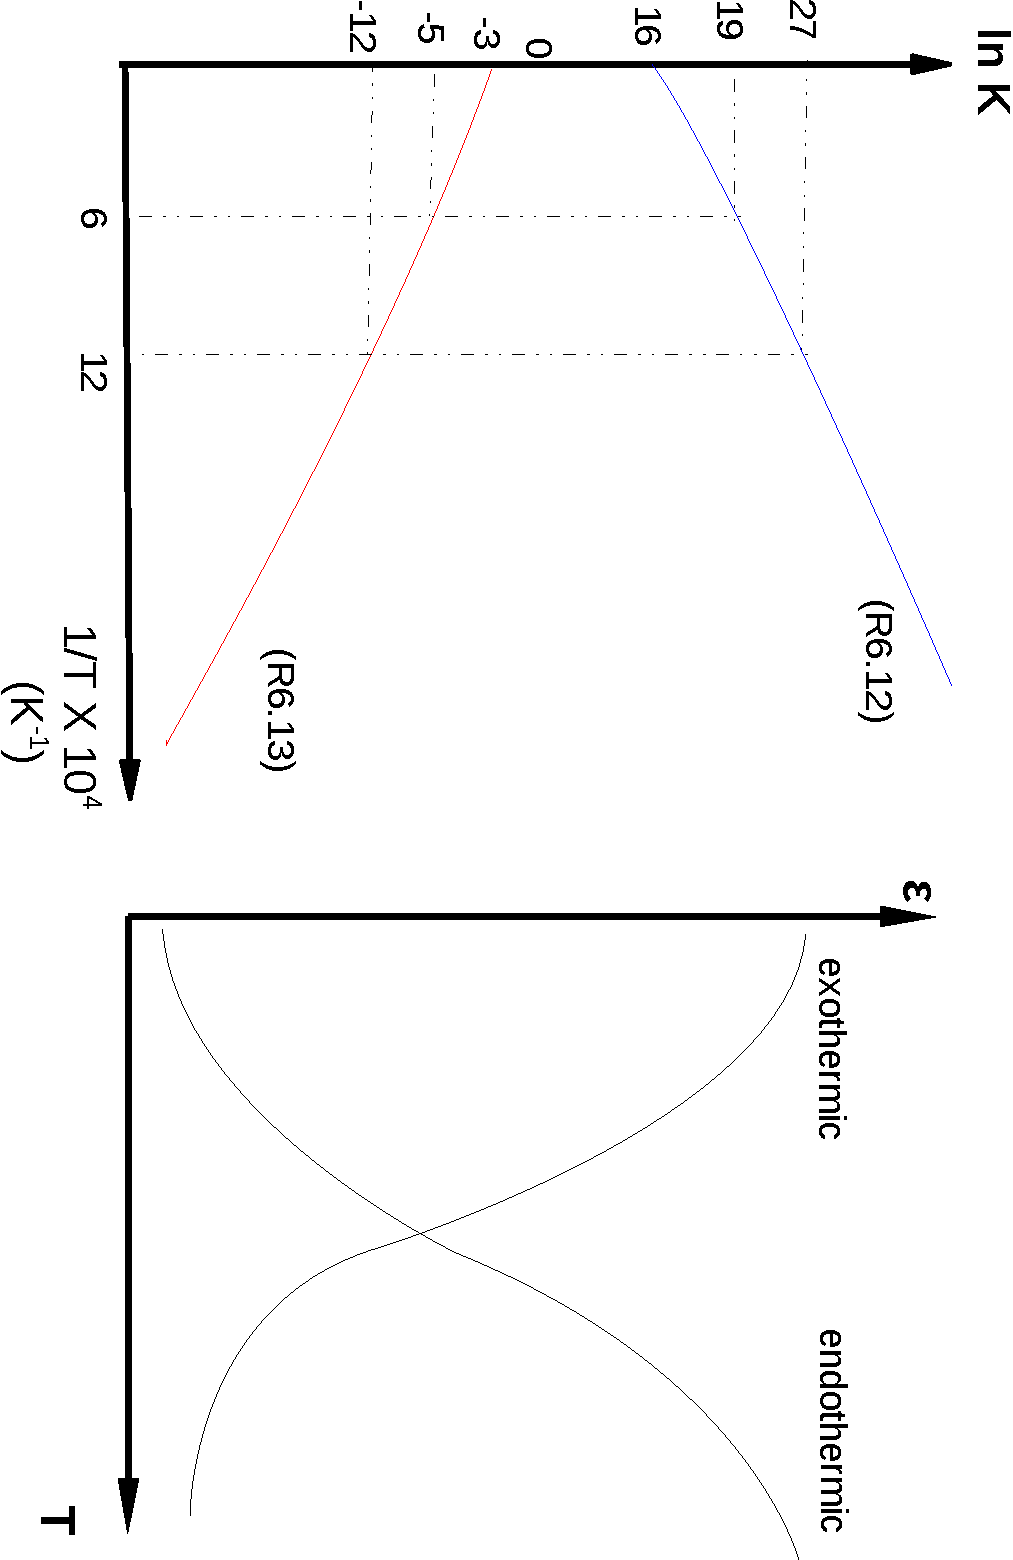
\includegraphics[width=0.5\columnwidth,angle=90,clip]{./Figs/Mod06_SchematicVantHoff_b}
           \caption{(Left) Sketch of equilibrium constants as a function of temperature for reactions~\ref{chemreaction:FormationCOb} and~\ref{chemreaction:FormationNO} \citep[data extracted from][]{SmithVanNess_Book}. (Right) Reaction coordinate $\times$ temperature -- qualitative analysis for endothermic/exothermic reactions based on the standard heat of reaction.}\label{Chapter:ChemicalReactions:Fig:Fig03}
         \end{center}
      \end{figure} 
     
      \begin{displaymath}
        \begin{cases}
            -\left[\frc{\Delta H^{\circ}}{R}\right]_{\ref{chemreaction:FormationCO}} =  \frc{27 - 19}{12-6} = 1.3333, &  \\
            -\left[\frc{\Delta H^{\circ}}{R}\right]_{\ref{chemreaction:FormationNO}} =  \frc{-12 - (-5)}{12-6} = -1.1667 &
          \end{cases}
      \end{displaymath}
      Reactions that present positive $\Delta H^{\circ}$ (\ie negative slope) are called {\it endothermic}, \ie equilibrium constant rises as the temperature is increased (or in other words, heat is given to the reactive system to promote the reaction). Similarly, negative $\Delta H^{\circ}$ (\ie positive slope) are called {\it exothermic}, \ie an increase in temperature leads to a decrease in the equilibrium constant (heat is transferred from the reactive system to the surroundings).

\begin{comment}
%%% SUBSECTION
\subsection{Dependence of $K$ with Temperature}\label{Chapter:ChemicalReactions:Section:K_Temperature}
%\begin{subequations}
    The fundamental thermodynamic relation for the Gibbs free energy at stadard state conditions,
       \begin{displaymath}
           G_{i}^{\circ} = H_{i}^{\circ} - TS_{i}^{\circ},
       \end{displaymath}
   can be extended to chemical reactions at standard state conditions (using Eqn.~\ref{Chapter:ChemicalReactions:Eqn:3b})
       \begin{equation}
           \underbrace{\summation[\nu_{i}G_{i}^{\circ}]{}{}}_{\Delta G^{\circ}} =  \underbrace{\summation[\nu_{i}H_{i}^{\circ}]{}{}}_{\Delta H^{\circ}} - T \underbrace{\summation[\nu_{i}S_{i}^{\circ}]{}{}}_{\Delta S^{\circ}},\label{Chapter:ChemicalReactions:Eqn:6a}
       \end{equation}
   where,
   \begin{enumerate}[i)]
       \item standard heat (enthalpy) of reaction $\left(\Delta H^{\circ}\right)$: starting from the definition of heat capacity at constant pressure, $C_{p}=\Partial[H]{T}{P}$, at standard conditions,
            \begin{eqnarray}
                 && dH_{i}^{\circ} = C_{p_{i}}^{\circ} dT \hspace{4cm}\blue{\left(\times \summation[\nu_{i}]{}{}\right)} \nonumber \\
                 && \summation[\nu_{i}dH_{i}^{\circ}]{}{} = \summation[\nu_{i}C_{p_{i}}^{\circ} dT]{}{} \nonumber \\
                 && \summation[d\left(\nu_{i}H_{i}^{\circ}\right)]{}{} = d\underbrace{\summation[\nu_{i}H_{i}^{\circ}]{}{}}_{\Delta H^{\circ}} = \underbrace{\summation[\nu_{i}C_{p_{i}}^{\circ}]{}{}}_{\Delta C_{p}^{\circ}}dT \nonumber \\
                 && \int d\left(\Delta H^{\circ}\right) = \int \Delta C_{p}^{\circ} dT \nonumber \\
                 && \Delta H^{\circ} - \Delta H^{\circ}_{0} = \blue{R}\int\limits_{T_{0}}^{T} \frc{\Delta C_{p}^{\circ}}{\blue{R}} dT \nonumber
            \end{eqnarray}
            here $R$ is acting as an {\it artifact} that will vanish in a later stage.

       \item standard entropy of reaction $\left(\Delta S^{\circ}\right)$: from the relation $\Partial[S]{T}{P}=\frc{C_{p}}{T}$,
            \begin{eqnarray}
                 && dS_{i}^{\circ} = C_{p_{i}}^{\circ} \frc{dT}{T} \nonumber \\
                 && \int d\left(\Delta S^{\circ}\right) = \int\limits_{T_{0}}^{T}\Delta C_{p}^{\circ}\frc{dT}{T} \nonumber \\
                 && \Delta S^{\circ} - \Delta S^{\circ}_{0} = \blue{R}\int\limits_{T_{0}}^{T}\frc{\Delta C_{p}^{\circ}}{\blue{R}} \frc{dT}{T} \nonumber 
            \end{eqnarray}
   \end{enumerate}
  Replacing these two terms in Eqn.~\ref{Chapter:ChemicalReactions:Eqn:6a} to obtain $\Delta G^{\circ}$
     \begin{eqnarray}
         \Delta G^{\circ} &=&  \Delta H^{\circ}_{0} + \blue{R}\int\limits_{T_{0}}^{T} \frc{\Delta C_{p}^{\circ}}{\blue{R}} dT - T\overbrace{\Delta S^{\circ}_{0}}^{\frc{\Delta H^{\circ}_{0}-\Delta G^{\circ}_{0}}{T_{0}}} - \blue{R}T\int\limits_{T_{0}}^{T}\frc{\Delta C_{p}^{\circ}}{\blue{R}} \frc{dT}{T} \;\;\;\;\; \blue{\times\left(\frc{1}{RT}\right)} \nonumber \\ 
         \underbrace{\frc{\Delta G^{\circ}}{RT}}_{-\ln{K}} &=&  \frc{\Delta G^{\circ}_{0}-\Delta H^{\circ}_{0}}{RT_{0}} + \frc{\Delta H^{\circ}_{0}}{RT} + \frc{1}{T}\int\limits_{T_{0}}^{T} \frc{\Delta C_{p}^{\circ}}{R}dT - \int\limits_{T_{0}}^{T}\frc{\Delta C_{p}^{\circ}}{R}dT \label{Chapter:ChemicalReactions:Eqn:6b}
     \end{eqnarray}
  The standard heat capacities, $\Delta C_{p}^{\circ}=\summation[\nu_{i}C_{p_{i}}^{\circ}]{}{}$ are often expressed as polynomials of the temperature for a range of chemical species. This ensures a sensitivity of this thermophysical parameter with respect to the temperature. In such cases, Eqn.~\ref{Chapter:ChemicalReactions:Eqn:6b} can only be solved numerically with the integrals ranging from the standard (or reference) temperature, $T_{0}$, to $T$. In addition, $\Delta G^{\circ}_{0}$ and $\Delta H^{\circ}_{0}$, Gibbs free energy and enthalpy of reaction at standard pressure conditions (\ie 1 atm) and at reference (or standad) temperature conditions (\ie 298.15 K) are tabulated and readily available in the literature for a number of (relatively) simple chemical reactions.

%\end{subequations}
\end{comment}

%%% SUBSECTION
\subsection{Dependence of $K$ with Composition}\label{Chapter:ChemicalReactions:Section:K_Composition}\index{Fugacity}\index{Fugacity! Coefficient}\index{Solutions!Activity coefficient}
    Recall that in Eqn.~\ref{Chapter:ChemicalReactions:Eqn:5b}, the equilibrium constant $K$ was defined as function of the activities of the reactive mixture,
    \begin{displaymath}
       K = \prod\limits_{i=1}^{\mathcal{C}} a_{i}^{\nu_{i}} = \prod\limits_{i=1}^{\mathcal{C}} \left(\frc{\overline{f}_{i}}{\overline{f}_{i}^{\circ}}\right)^{\nu_{i}}.
    \end{displaymath}
    As the standard state of a gas is the ideal gas state at $P^{\circ}=1\text{ atm}$, the fugacity of an ideal gas in the standard state is equal to its pressure $\overline{f}_{i}^{\circ}=P^{\circ}$ for each reactive species $i$, thus
    \begin{displaymath}
       K = \prod\limits_{i=1}^{\mathcal{C}} \left(\frc{\overline{f}_{i}}{P^{\circ}}\right)^{\nu_{i}},
    \end{displaymath}
    however, for the gaseous phase $\overline{f}_{i} = \overline{\phi}_{i}y_{i}P$,
    \begin{displaymath}
        K = \prod\limits_{i=1}^{\mathcal{C}} \left(\frc{\overline{\phi}_{i}y_{i}P}{P^{\circ}}\right)^{\nu_{i}} = \left[\prod\limits_{i=1}^{\mathcal{C}} \left(\overline{\phi}_{i}y_{i}\right)^{\nu_{i}}\right]\left(\frc{P}{P^{\circ}}\right)^{\summation[\nu_{i}]{i}{} }.
    \end{displaymath}
    \begin{shaded}    
       \noindent Defining $\nu=\summation[\nu_{i}]{i}{}$,
       \begin{equation}
           \prod\limits_{i=1}^{\mathcal{C}} \left(\overline{\phi}_{i}y_{i}\right)^{\nu_{i}} = K\left(\frc{P}{P^{\circ}}\right)^{-\nu}\;\;\;\;\blue{\text{ (for gaseous phase).}}\label{Chapter:ChemicalReactions:Eqn:5d}
       \end{equation}
       At low pressure or high temperature, the fluid behaves as an ideal gas, \ie $\overline{\phi}_{i}=1$, thus
       \begin{equation}
           \prod\limits_{i=1}^{\mathcal{C}} y_{i}^{\nu_{i}} = K\left(\frc{P}{P^{\circ}}\right)^{-\nu}\;\;\;\;\blue{\text{ (for ideal gases).}}\label{Chapter:ChemicalReactions:Eqn:5e}
       \end{equation}
    \end{shaded}
    Now, for the liquid phase the expression previously defined 
    \begin{displaymath}
       K = \prod\limits_{i=1}^{\mathcal{C}} \left(\frc{\overline{f}_{i}}{\overline{f}_{i}^{\circ}}\right)^{\nu_{i}},
    \end{displaymath}
    still holds, and for {\it pure liquid} $i$ at $T$ and 1 atm, using $\overline{f}_{i} = \gamma_{i}x_{i}f_{i}$ (Eqn.~\ref{Chapter:SolutionThermodynamics:Eqn:activity1g}), where $f_{i}$ is the fugacity of pure component $i$ in the liquid phase at $P$ and $T$. Hence,
    \begin{displaymath}
       \frc{\overline{f}_{i}}{\overline{f}_{i}^{\circ}} = \frc{\gamma_{i}x_{i}f_{i}}{\overline{f}_{i}^{\circ}} = \gamma_{i}x_{i}\left(\frc{f_{i}}{\overline{f}_{i}^{\circ}}\right).
    \end{displaymath}
    The fugacity ratio in brackets can be obtained by manipulating the Maxwell relation, $\Partial[G]{P}{T}=V$, and integrating from standard state to $T$ and $P$,
    \begin{eqnarray}
          G_{i}-G_{i}^{\circ} &=& \int\limits_{P^{\circ}}^{P}V_{i}dP \nonumber  \\
          RT\ln{\left(\frc{f_{i}}{f_{i}^{\circ}}\right)} &=& \int\limits_{P^{\circ}}^{P}V_{i}dP \;\;\;\Longrightarrow\;\;\; \ln{\left(\frc{f_{i}}{f_{i}^{\circ}}\right)} = \frc{V_{i}\left(P-P^{\circ}\right)}{RT}, \nonumber
    \end{eqnarray}
    assuming that fluids at liquid phase are incompressible $\left(\text{\ie } V_{i} \text{ is constant}\right)$. Now, replacing in the original equation\footnote{Here, properties of exponents (see Appendix~\ref{Chapter:LogExpReview:Section:Exp}) are used to operate over the thermodynamic properties. Given the set of reals $a_{i}$ and $b_{i}$ $\forall i\in\left\{1,2,\cdots, z\right\}$ and constants $c$ and $d$:
   \begin{enumerate}[a)]
       \item $\left(e^{c}\right)^{d} = e^{cd}$;
       \item $e^{a_{1}b_{1}c}\cdot e^{a_{2}b_{2}c}\cdots e^{a_{z}b_{z}c} = e^{c\left(a_{1}b_{1}+a_{2}b_{2}+\cdots+a_{z}b_{z}\right)}$.
   \end{enumerate}
},
    \begin{eqnarray}
          K &=& \prod\limits_{i=1}^{\mathcal{C}} \left(\frc{\overline{f}_{i}}{\overline{f}_{i}^{\circ}}\right)^{\nu_{i}} = \prod\limits_{i=1}^{\mathcal{C}} \left[\gamma_{i}x_{i}\left(\frc{f_{i}}{\overline{f}_{i}^{\circ}}\right)\right]^{\nu_{i}} \nonumber \\
            &=& \prod\limits_{i=1}^{\mathcal{C}} \left[\gamma_{i}x_{i}\exp{\left(\frc{V_{i}\left(P-P^{\circ}\right)}{RT}\right)}\right]^{\nu_{i}}  = \prod\limits_{i=1}^{\mathcal{C}}\left(\gamma_{i}x_{i}\right)^{\nu_{i}} \times \left\{\exp{\left[\summation[\frc{V_{i}\left(P-P^{\circ}\right)}{RT}]{i}{}\right]}\right\}^{\nu_{i}} \nonumber \\
            &=& \prod\limits_{i=1}^{\mathcal{C}}\left(\gamma_{i}x_{i}\right)^{\nu_{i}} \times \exp{\left[\frc{P-P^{\circ}}{RT}\summation[V_{i}\nu_{i}]{i=1}{\mathcal{C}}\right]}\nonumber
    \end{eqnarray}
    \begin{shaded}
       \begin{equation}
           \prod\limits_{i=1}^{\mathcal{C}}\left(\gamma_{i}x_{i}\right)^{\nu_{i}} = K\exp{\left[\frc{P^{\circ}-P}{RT}\summation[V_{i}\nu_{i}]{i=1}{\mathcal{C}}\right]}\;\;\;\;\blue{\text{ (for liquid phase).}}\label{Chapter:ChemicalReactions:Eqn:5f}
       \end{equation}
       Simplifications:
       \begin{enumerate}[a)]
           \item At room pressure conditions, $P^{\circ}-P=0$ and
              \begin{equation}
                 K = \prod\limits_{i=1}^{\mathcal{C}}\left(\gamma_{i}x_{i}\right)^{\nu_{i}} \;\;\;\;\blue{\text{ (for liquid phase at room pressure conditions).}}\label{Chapter:ChemicalReactions:Eqn:5g}
              \end{equation}
              Although at first sight this equation may seem relatively simple to solve, activity coefficient models are often necessary to be used making it complex to solve, in such cases iterative methods are commonly employed;
           \item For ideal solutions, $\gamma=1$ and Eqn.~\ref{Chapter:ChemicalReactions:Eqn:5g} becomes,
              \begin{equation}
                 K = \prod\limits_{i=1}^{\mathcal{C}}x_{i}^{\nu_{i}} \;\;\;\;\blue{\text{ (for ideal solutions).}}\label{Chapter:ChemicalReactions:Eqn:5h}
              \end{equation}              
       \end{enumerate}
    \end{shaded}
     
\end{subequations}


%%% SECTION
\section{Equilibrium Constant in Multiple Simultaneous Reactions}\label{Chapter:ChemicalReactions:Section:MultipleReactions}
\begin{subequations}
  Calculations of equilibrium constant of single homogeneous chemical reactions can be extended to multiple independent reactions. Let's consider a set of $\mathcal{R}$ independent reactions involving $\mathcal{C}$ chemical species, the equilibrium constant for each reaction is given by an extension of Eqn.~\ref{Chapter:ChemicalReactions:Eqn:5b}
  \begin{shaded}
    \begin{equation}
        K_{j} = \prod\limits_{i=1}^{\mathcal{C}} \left(\frc{\overline{f}_{i}}{\overline{f}_{i}^{\circ}}\right)^{\nu_{i,j}},\;\;\;\;\forall j\in\left\{1,2,\cdots,\mathcal{R}\right\}.\label{Chapter:ChemicalReactions:Eqn:6a}
    \end{equation}
  \end{shaded}
  For {\it gaseous} reactions,
  \begin{shaded}
    \begin{equation}
      K_{j} =
      \begin{cases}
          \prod\limits_{i=1}^{\mathcal{C}} \left(\frc{\overline{f}_{i}}{P^{\circ}}\right)^{\nu_{i,j}},\;\;\;\;\blue{\text{(gas phase),}}\label{Chapter:ChemicalReactions:Eqn:6b} \\
           \\
          \left(\frc{P}{P^{\circ}}\right)^{-\nu_{i,j}}\prod\limits_{i=1}^{\mathcal{C}} \left(y_{i}\right)^{\nu_{i,j}},\;\;\;\;\blue{\text{(ideal gas mixture).}}
      \end{cases}
      \forall j\in\left\{1,2,\cdots,\mathcal{R}\right\}
    \end{equation}
  \end{shaded}



\end{subequations}


\clearpage

%%% SECTION
\section{Examples}

\begin{enumerate}[1)]

%%%
%%% Elliot & Lira (Ex 3.4)  
%%%
\item\label{Example:1} Five moles of hydrogen, two moles of CO and 1.5 moles of CH$_{3}$OH vapour are combined in a batch methanol synthesis reactor (closed system) at 500 K and 1 MPa. Develop expressions for the mole fractions of the species in terms of the reaction coordinate. The components are known to react with the following stoichiometry:
  \begin{displaymath}
      2 H_{2} (g) + CO (g) \Longleftrightarrow CH_{3}OH (g).
  \end{displaymath}

\bigskip

{\bf Solution:} We need to develop expressions for each species in the gaseous form. In the equilibrium, the molar stoichiometric coefficient and the initial number of moles are:
    \begin{displaymath}
       \begin{cases}
         \nu = \sum\limits_{i}\nu_{i}= (-2)+(-1)+(+1)= -2 \;\;\text{ and } \\
         n_{0} = \sum\limits_{i}n_{i,0}= 5 + 2 + 1.5 = 8.5,
       \end{cases}
    \end{displaymath} 
    respectively. Mole fraction of each species is given by
    \begin{displaymath}
          y_{i} = \frc{n_{i}}{n} = \frc{n_{i,0}+\nu_{i}\epsilon}{n_{0}+\nu\epsilon},
    \end{displaymath}
    where the the total number of moles in equilibrium is $n=8.5-2\epsilon$, thus
    \begin{displaymath}
       \begin{cases}
         y_{\text{H}_{2}} = \frc{5-2\epsilon}{8.5-2\epsilon}, \\
         \\
         y_{\text{CO}} = \frc{2-\epsilon}{8.5-2\epsilon}\\
         \\
          y_{\text{CH}_{3}\text{OH}}=\frc{1.5+\epsilon}{8.5-2\epsilon}
       \end{cases}
    \end{displaymath}
\clearpage

\begin{comment}
%%%
%%%   
%%%
\item\label{Example:2} Consider the chemical reaction,
         \begin{displaymath}
             C_{2}H_{4} (g) + H_{2}O (g) \Longleftrightarrow  C_{2}H_{5}OH (g).
         \end{displaymath}
         If an equimolar mixture of ethylene and water vapour is fed to a reactor which is maintained at 500 K and 40 bar, determine the equilibrium constant, assuming that the reaction mixture behaves like an ideal gas. Assume the following ideal gas specific heat data:
         \begin{displaymath}
             C_{p}^{\text{ig}} = a + bT + cT^{2} + dT^{3} + eT^{-2},
         \end{displaymath}
         where C$_{p}^{\text{ig}}$ is expressed in {\it J/mol} and $T$ in $K$. Also,
         \begin{center}
            \begin{tabular}{|c|c c c c c|}
                \hline
                {\it Species}    & $a$    &  $b\times 10^{3}$  & $c\times 10^{6}$ & $d\times 10^{9}$  & $e\times10^{-5}$ \\
                \hline
                C$_{2}$H$_{4}$    & 20.691 &   205.346          & -99.793         & 18.825           & --               \\
                H$_{2}$O         & 4.196  &  154.565           & -81.076         &  16.813          & --               \\
                C$_{2}$H$_{5}$OH  & 28.850 &  12.055            & --              &  --              & 1.006           \\
                \hline
            \end{tabular}
         \end{center}
         The standard state enthalpy and Gibbs energy of reaction are $\Delta H^{0}_{\text{R},298}=-52.7$ kJ/mol and $\Delta G^{0}_{\text{R},298}=14.5$ kJ/mol. In order to calculate the enthalpy of reaction at temperature $T$, $\Delta H^{0}_{T}$, you should use,
         \begin{displaymath}
            \Delta H^{0}_{T} = \Delta H^{0}_{\text{R},298} + \int\limits_{T_{0}}^{T} \Delta C_{p} dT = \Delta H^{0}_{\text{R},298} + \int\limits_{T_{0}}^{T}\left(\Delta a + \Delta bT + \Delta cT^{2} + \Delta dT^{3} + \Delta eT^{-2}\right) dT
         \end{displaymath} 
         where $\Delta a= \sum\limits_{i} \nu_{i}a_{i}$, $\Delta b= \sum\limits_{i} \nu_{i}b_{i}$, $\Delta c= \sum\limits_{i} \nu_{i}c_{i}$, $\Delta d= \sum\limits_{i} \nu_{i}d_{i}$ and $\Delta e= \sum\limits_{i} \nu_{i}e_{i}$.  Also, given the Van't Hoff equation:
         \begin{displaymath}
            \frc{d}{dT}\left(\Delta G^{0}/RT\right) = -\frc{\Delta H^{0}}{RT^{2}}.
         \end{displaymath}


\bigskip

{\bf Solution:}

   \begin{itemize}
      \item We first need to obtain the integral expression for the heat of reaction at temperature $T$,
         \begin{displaymath}
            \Delta H^{0}_{T} = \Delta H^{0}_{\text{R},298} + \int\limits_{T_{0}}^{T} \Delta C_{p} dT = \Delta H^{0}_{\text{R},298} + \int\limits_{T_{0}}^{T}\left(\Delta a + \Delta bT + \Delta cT^{2} + \Delta dT^{3} + \Delta eT^{-2}\right) dT
         \end{displaymath} 
         with 
         \begin{center}
             \begin{tabular}{r l c}
                $\Delta a =$ & $(+1).(28.850)-\left[(-1).(20.691)+(-1).(4.196)\right]=$ & 3.963 \\
                $\Delta b =$ & $\left\{(+1).(12.055)- \left[(-1).(205.346)+(-1).(154.565)\right]\right\}\times 10^{-3}=$ & 0.37197 \\
                $\Delta c =$ & $\left\{(+1).(0)-\left[(-1).(-99.793)+(-1).(-81.076)\right]\right\}\times 10^{-6}=$       & -1.8087$\times$10$^{-4}$  \\
                $\Delta d =$ & $\left\{(+1).(0)-\left[(-1).(18.825)+(-1).(16.813)\right]\right\}\times 10^{-9}=$         & 3.5638$\times$10$^{-8}$\\
                $\Delta e =$ & $\left\{(+1).(1.006)-\left[(-1).(0)+(-1).(0)\right]\right\}\times 10^{5}=$                & 1.006$\times$10$^{5}$ \\
             \end{tabular}
         \end{center}
         Thus,
         \begin{eqnarray}
            \Delta H^{0}_{T} &=& \Delta H^{0}_{\text{R},298} + \int\limits_{T_{0}}^{T} \Delta C_{p} dT = \Delta H^{0}_{\text{R},298} + \int\limits_{T_{0}}^{T}\left(\Delta a + \Delta bT + \Delta cT^{2} + \Delta dT^{3} + \Delta eT^{-2}\right) dT \nonumber \\
            &=& -52.7 + \int\limits_{T_{0}}^{T} \left(3.963 + 0.37197 T - 1.8087\times 10^{-4} T^{2} + 3.5638\times 10^{-8} T^{3} + \frc{1.006 \times 10^{5}}{T^{-2}} \right)dT \nonumber
         \end{eqnarray}
%
      \item We can calculate the Gibbs energy of the reaction through the Van't Hoff equation:
         \begin{displaymath}
                \frc{d}{dT}\left(\Delta G^{0}/RT\right) = -\frc{\Delta H^{0}}{RT^{2}}.
         \end{displaymath}
         Integrating this equation from the standard state temperature, 298.15 K, to $T=$ 500 K

          
   \end{itemize}
\clearpage
\end{comment}

%%%
%%%   Nguyen (Ex 6.6.1)  
%%%
\item\label{Example:2} Ethylene is produced from the decomposition of ethane,
       \begin{displaymath}
          C_{2}H_{6} (g) \Longleftrightarrow C_{2}H_{4} (g) + H_{2} (g) 
       \end{displaymath} 
       Determine the equilibrium composition at 1000$^{\circ}$C and 1 atm. Assume that, initially, there is 1 mol of ethane. Given,
       \begin{center}
           \begin{tabular}{|c c c c|}
           \hline
                                        &  C$_{2}$H$_{6}$ (g) & C$_{2}$H$_{4}$ (g) &  H$_{2}$ (g)  \\ 
           \hline
             $\Delta G^{\circ}_{\text{f,298}}$  &  -32.84            &  68.15           & 0.0           \\
                   (kJ/mol)             &                    &                  &               \\
           \hline
             $\Delta H^{\circ}_{\text{f,298}}$  &  -84.68            &  52.26           & 0.0           \\
                   (kJ/mol)             &                    &                  &               \\
           \hline 
           \end{tabular}
       \end{center}
       where $\Delta G^{\circ}_{\text{f,298}}$ and $\Delta H^{\circ}_{\text{f,298}}$ are the standard state Gibbs energy and enthalpy of formation. 

\bigskip

{\bf Solution:} First we need to determine the standard state Gibbs energy of reaction,
         \begin{eqnarray}
             \Delta G^{\circ}_{\text{r,298}} &=& \sum\limits_{i}\nu_{i}\left(\Delta G^{\circ}_{\text{f,298}}\right)_{i} \nonumber \\
                                     &=& (+1).(68.15)+ (1).(0.0) + (-1).(-32.84) = 100.99\; \text{kJ/mol} \nonumber
         \end{eqnarray}
       The equilibrium constant can be obtained from,
         \begin{displaymath}
            K = \exp\left(-\frc{\Delta G^{\circ}_{\text{r,298}}}{RT}\right) = exp\left(-\frc{100.99\times 10^{3}}{(8.314).(298.15)}\right) = 2.0246\times 10^{-18}
         \end{displaymath}
       The Van't Hoff equation can be used to calculate the equilibrium constant at temperature $T$,
         \begin{displaymath}
            \frc{\partial\left(\ln K\right)}{\partial T} = \frc{\Delta H^{\circ}_{\text{r}}}{RT^{2}}
         \end{displaymath}
       Before we can integrate the Van't Hoff equation, we first need to determine the standard heat of reaction, $\Delta H^{\circ}_{\text{r}}$,
         \begin{eqnarray}
            \Delta H^{\circ}_{\text{r}} &=& \sum\limits_{i} \nu_{i}\left(\Delta H^{\circ}_{\text{f,298}}\right)_{i} \nonumber \\
                                 &=& (+1).(52.26) + (+1).(0.0) + (-1).(-84.68) = 136.94\;\text{kJ/mol}\nonumber
         \end{eqnarray}
       Now integrating the Van't Hoff equation from 298.15 K to 1273.15 K,
         \begin{eqnarray}
            \ln\frc{K_{1273}}{K_{298}} &=& -\frc{\Delta H^{\circ}_{\text{r}}}{R}\left(\frc{1}{T}-\frc{1}{298.15}\right) \nonumber \\
            \ln\frc{K_{1273}}{2.0246\times 10^{-18}} &=& -\frc{136.94\times 10^{3}}{8.314}\left(\frc{1}{1273.15}-\frc{1}{298.15}\right) \nonumber \\
            K_{1273} &=& 4.7859 \nonumber
         \end{eqnarray} 
       The equilibrium constant $K$ can also be expressed as a function of the components' activities,
         \begin{displaymath}
            K = \prod\limits_{i=1}^{\mathcal{C}} a_{i}^{\nu_{i}} = \frc{a_{\text{C}_{2}\text{H}_{4}}a_{\text{H}_{2}}}{a_{\text{C}_{2}\text{H}_{6}}} = \frc{\left(\frc{\overline{f}_{\text{C}_{2}\text{H}_{4}}}{\overline{f}^{\circ}_{\text{C}_{2}\text{H}_{4}}}\right)\left(\frc{\overline{f}_{\text{H}_{2}}}{\overline{f}^{\circ}_{\text{H}_{2}}}\right)}{\left(\frc{\overline{f}_{\text{C}_{2}\text{H}_{6}}}{\overline{f}^{\circ}_{\text{C}_{2}\text{H}_{6}}}\right)}
         \end{displaymath}
         Assuming ideal gas behaviour, $\overline{f}_{i}=P_{i}$, $\overline{f}_{i}^{\circ}=P^{\circ}_{\text{C}_{2}\text{H}_{6}}=P^{\circ}_{\text{C}_{2}\text{H}_{4}}=P^{\circ}_{\text{H}_{2}}=$ 1 atm. Thus,
         \begin{displaymath}
            K = \frc{a_{\text{C}_{2}\text{H}_{4}}a_{\text{H}_{2}}}{a_{\text{C}_{2}\text{H}_{6}}} = \frc{\left(\frc{\overline{f}_{\text{C}_{2}\text{H}_{4}}}{\overline{f}^{\circ}_{\text{C}_{2}\text{H}_{4}}}\right)\left(\frc{\overline{f}_{\text{H}_{2}}}{\overline{f}^{\circ}_{\text{H}_{2}}}\right)}{\left(\frc{\overline{f}_{\text{C}_{2}\text{H}_{6}}}{\overline{f}^{\circ}_{\text{C}_{2}\text{H}_{6}}}\right)} = \frc{\left(\frc{P_{\text{C}_{2}\text{H}_{4}}}{P^{\circ}_{\text{C}_{2}\text{H}_{4}}}\right)\left(\frc{P_{\text{H}_{2}}}{P^{\circ}_{\text{H}_{2}}}\right)}{\left(\frc{P_{\text{C}_{2}\text{H}_{6}}}{P^{\circ}_{\text{C}_{2}\text{H}_{6}}}\right)} = \frc{\left(\frc{y_{\text{C}_{2}\text{H}_{4}}P}{1\text{ atm}}\right)\left(\frc{y_{\text{H}_{2}}P}{1\text{ atm}}\right)}{\left(\frc{y_{\text{C}_{2}\text{H}_{6}}P}{1\text{ atm}}\right)}          
         \end{displaymath}
         Since $P=$ 1 atm,
         \begin{displaymath}
            K = \frc{\left(\frc{y_{\text{C}_{2}\text{H}_{4}}P}{1\text{ atm}}\right)\left(\frc{y_{\text{H}_{2}}P}{1\text{ atm}}\right)}{\left(\frc{y_{\text{C}_{2}\text{H}_{6}}P}{1\text{ atm}}\right)} = \frc{\left(y_{\text{C}_{2}\text{H}_{4}}\right)\left(y_{\text{H}_{2}}\right)}{\left(y_{\text{C}_{2}\text{H}_{6}}\right)} = 4.7859
         \end{displaymath}
         This equation can not be solved as there are two unknowns $\left(\text{remember that }\summation[y_{i}]{i=1}{3}=1\right)$. The number of unknowns can be decreased if we make use of
         \begin{displaymath}
           y_{i} = \frc{n_{i}}{n} = \frc{n_{i,0}+\nu_{i}\epsilon}{n_{0}+\nu\epsilon}.
         \end{displaymath}
         with 
         \begin{displaymath}
            \nu = \sum\limits_{i}\nu_{i}= (-1)+(+1)+(+1)= 1 \;\;\text{ and }\;\; n_{0} = \sum\limits_{i}n_{i,0}= 1 + 0 + 0 = 1,
         \end{displaymath} 
       Thus,
         \begin{displaymath}
             y_{\text{C}_{2}\text{H}_{6}} = \frc{1-\epsilon}{1+\epsilon},\;\;y_{\text{C}_{2}\text{H}_{4}} = \frc{\epsilon}{1+\epsilon}\;\text{ and }\;y_{\text{H}_{2}} = \frc{\epsilon}{1+\epsilon}
         \end{displaymath}
       Replacing the compositions in the expression for $K$,
         \begin{eqnarray}
           K  &=& \frc{\left(y_{\text{C}_{2}\text{H}_{4}}\right)\left(y_{\text{H}_{2}}\right)}{\left(y_{\text{C}_{2}\text{H}_{6}}\right)} = \frc{\left(\frc{\epsilon}{1+\epsilon}\right)^{2}}{\left(\frc{1-\epsilon}{1+\epsilon}\right)} =4.7859 \nonumber \\
            &&\epsilon = 0.9095 \nonumber
         \end{eqnarray}
        The equilibrium concentration of C$_{2}$H$_{4}$(g) is $y_{\text{C}_{2}\text{H}_{4}} =$ 0.4763 $=y_{\text{H}_{2}}$ and $y_{\text{C}_{2}\text{H}_{6}}=$ 0.0474.

\clearpage


%%%
%%%   Nguyen (Ex 6.7.2) 
%%%
\item\label{Example:3} Determine the equilibrium conversion for the liquid-phase isomerisation reaction of methylcyclopentane $\left(\text{CH}_{3}\text{C}_{5}\text{H}_{9}\right)$ to cyclohexane $\left(\text{C}_{6}\text{H}_{12}\right)$ at 25$^{\circ}$C. Gibbs energies of formation are given at 25$^{\circ}$C as:
  \begin{displaymath}
     \left(\Delta G^{\circ}_{\text{f,298}}\right)_{\text{CH}_{3}\text{C}_{5}\text{H}_{9}} = 31.72 \text{ kJ.mol}^{-1} \text{ and } \left(\Delta G^{\circ}_{\text{f,298}}\right)_{\text{C}_{6}\text{H}_{12}} = 26.89 \text{ kJ.mol}^{-1}.
  \end{displaymath}
  Also, assume that this isomerisation reaction occurs at relatively low pressure, and therefore $\frc{f_{i}}{f^{\circ}_{i}}=1$. Also, assume that solution is ideal.


\bigskip

{\bf Solution:} The isomerisation reaction can be represented by,
    \begin{displaymath}
        CH_{3}C_{5}H_{9} (l) \Longleftrightarrow C_{6}H_{12} (l)
    \end{displaymath}
    We need to determine the equilibrium constant at room temperature
         \begin{eqnarray}
           \Delta G^{\circ}_{r,298} &=& \sum\limits_{i}\nu_{i}\Delta G^{\circ}_{\text{f,298}} \nonumber \\
                             &=& (+1).\left(\Delta G^{\circ}_{\text{f,298}}\right)_{\text{C}_{6}\text{H}_{12}} + (-1).\left(\Delta G^{\circ}_{\text{f,298}}\right)_{\text{CH}_{3}\text{C}_{5}\text{H}_{9}} \nonumber \\ 
                             &=& 26.89-31.72 = -4.83 \text{ kJ/mol} \nonumber
         \end{eqnarray}
       The equilibrium constant is
         \begin{displaymath}
             K = \exp\left(-\frc{\Delta G^{\circ}_{r,298}}{RT}\right) = \exp\left(-\frc{-4830}{(8.314).(298.15)}\right) = 7.0182
         \end{displaymath}
       The equilibrium constant can also be obtained from 
         \begin{displaymath}
            K = \prod\limits_{i}\left(\frc{\overline{f}_{i}}{\overline{f}^{\circ}_{i}}\right)^{\nu_{i}} = \prod\limits_{i}\left(\frc{x_{i}\gamma_{i} f_{i}}{\overline{f}^{\circ}_{i}}\right)^{\nu_{i}}
         \end{displaymath}
       At room pressure conditions, the ratio $\frc{f_{i}}{\overline{f}^{\circ}_{i}} = \frc{f_{i}}{f_{i}^{\circ}} = \exp\left[\frc{V\left(P-P^{\circ}\right)}{RT}\right]=1$, therefore,
         \begin{displaymath}
            K = \prod\limits_{i}\left(\frc{x_{i}\gamma_{i}f_{i}}{\overline{f}^{\circ}_{i}}\right)^{\nu_{i}} = \prod\limits_{i}\left(x_{i}\gamma_{i}\right)^{\nu_{i}}
         \end{displaymath}
       For ideal solution,
         \begin{displaymath}
            K = \prod\limits_{i=1}^{\mathcal{C}}\left(x_{i}\gamma_{i}\right)^{\nu_{i}} = \prod\limits_{i}\left(x_{i}\right)^{\nu_{i}} = \left(x_{\text{C}_{6}\text{H}_{12}}\right).\left(x_{\text{CH}_{3}\text{C}_{5}\text{H}_{9}}\right)^{-1} = 7.0182,
         \end{displaymath}
         as $\summation[x_{i}]{i}{}=1$, we could easily solve the equation above as $x_{\text{C}_{6}\text{H}_{12}}\left(1-x_{\text{C}_{6}\text{H}_{12}}\right)=7.0182$, and obtain $x_{\text{C}_{6}\text{H}_{12}}=0.8753$. Alternatively, one could obtain a relation between composition and the reaction coordinate, $\varepsilon$,
         \begin{displaymath}
            x_{i} = \frc{n_{i,0} + \nu_{i}\varepsilon}{n_{0}+\nu\epsilon},
         \end{displaymath}
         where $\nu = (-1) + (1) = 0$ and assuming that initially there are $n_{\text{CH}_{3}\text{C}_{5}\text{H}_{9},0}=1$ and $n_{\text{C}_{6}\text{H}_{12},0}=0$,
         \begin{displaymath}
            x_{\text{CH}_{3}\text{C}_{5}\text{H}_{9}} = 1-\varepsilon\;\;\;\;\;\text{ and }\;\;\;\;\;\; x_{\text{C}_{6}\text{H}_{12}} = \varepsilon.
         \end{displaymath}
         Now, replacing in the expression above, 
         \begin{displaymath}
             K = \left(x_{\text{C}_{6}\text{H}_{12}}\right).\left(x_{\text{CH}_{3}\text{C}_{5}\text{H}_{9}}\right)^{-1} = \frc{\varepsilon}{1-\varepsilon} = 7.0182 \;\;\;\; \Longrightarrow \;\;\;\;\; \epsilon = 0.8753 
         \end{displaymath}
         Thus, $x_{\text{C}_{6}\text{H}_{12}}=0.8753$ and $x_{\text{CH}_{3}\text{C}_{5}\text{H}_{9}}=0.1247$.

\clearpage

%%%
%%%  Sandler (Ex 13.1.1, pg. 713)
%%%
\item\label{Example:4} Calculate the equilibrium extent of decomposition of nitrogen tetroxide $\left(N_{2}O_{4}\right)$,
  \begin{displaymath}
     N_{2}O_{4} (g) \Longleftrightarrow 2 NO_{2} (g)
  \end{displaymath}
  at 298.15 K and 1 atm. Assume that the gas mixture behaves as an ideal gas and the Gibbs energies of formation at 25$^{\circ}$C are:
  \begin{displaymath}
     \left(\Delta G^{\circ}_{\text{f,298}}\right)_{N_{2}O_{4}} = 97.89 \text{ kJ.mol}^{-1} \text{ and } \left(\Delta G^{\circ}_{\text{f,298}}\right)_{NO_{2}} = 51.31 \text{ kJ.mol}^{-1}.
  \end{displaymath}
     

\bigskip

{\bf Solution:} 
       The equilibrium constant is
         \begin{displaymath}
             K = \exp\left(-\frc{\Delta G^{\circ}_{r,298}}{RT}\right) = \frc{a_{NO_{2}}^{2}}{a_{N_{2}O_{4}}} = \frc{\left(\frc{y_{NO_{2}}P}{P^{\circ}_{NO_{2}}}\right)^{2}}{\left(\frc{y_{N_{2}O_{4}}P}{P^{\circ}_{N_{2}O_{4}}}\right)} = \frac{\left(y_{NO_{2}}\right)^{2}}{\left(y_{N_{2}O_{4}}\right)},
         \end{displaymath}
         where the standard Gibbs energy of reaction is
         \begin{eqnarray}
           \Delta G^{\circ}_{r,298} &=& \sum\limits_{i}\nu_{i}\Delta G^{\circ}_{\text{f,298}} \nonumber \\
                             &=& (+2).\left(\Delta G^{\circ}_{\text{f,298}}\right)_{NO_{2}} + (-1).\left(\Delta G^{\circ}_{\text{f,298}}\right)_{N_{2}O_{4}} \nonumber \\ 
                             &=& 4730 \text{ J/mol}, \nonumber
         \end{eqnarray}
         and the equilibrium constant,
         \begin{displaymath}
             K = \exp\left(-\frc{\Delta G^{\circ}_{r,298}}{RT}\right) = 0.1484 = \frac{\left(y_{NO_{2}}\right)^{2}}{\left(y_{N_{2}O_{4}}\right)}
         \end{displaymath}
         Composition and reaction coordinate are related through
         \begin{displaymath}
            y_{i} = \frc{n_{i,0} + \nu_{i}\varepsilon}{n_{0}+\nu\epsilon},
         \end{displaymath}
         where, assuming that the initial number of moles are $n_{N_{2}O_{4},0}=1$ and $n_{NO_{2},0}=0$, an $\nu= 2-1 = 1$,
         \begin{displaymath}
            y_{N_{2}O_{4}} = \frc{1-\varepsilon}{1+\varepsilon}\;\;\;\;\;\text{ and }\;\;\;\;\;\; y_{NO_{2}} = \frc{2\varepsilon}{1+\varepsilon},
         \end{displaymath}
         leading to
         \begin{displaymath}
             K = \frac{\left(y_{NO_{2}}\right)^{2}}{\left(y_{N_{2}O_{4}}\right)} = \frc{\left(\frc{2\varepsilon}{1+\varepsilon}\right)^{2}}{\left(\frc{1-\varepsilon}{1+\varepsilon}\right)} = 0.1484 \;\;\;\;\Longrightarrow\;\;\;\; \varepsilon = 0.1891
         \end{displaymath}
         Thus: $y_{NO_{2}} = 0.3181$ and $y_{N_{2}O_{4}} = 0.6819$.

         
\clearpage

%%%
%%%  Sandler (Ex 13.1.2, pg. 714)
%%%
\item\label{Example:5} Pure nitrogen tetroxide $\left(N_{2}O_{4}\right)$ at a low temperature is diluted with nitrogen $\left(N_{2}\right)$ and heated to 298.15 K and 1 atm. If the initial mole fraction of $N_{2}O_{4}$ in the $N_{2}O_{4}-N_{2}$ mixture before the dissociation begins is 0.20, what is the extent of the decomposition, 
  \begin{displaymath}
     N_{2}O_{4} (g) \Longleftrightarrow 2 NO_{2} (g)
  \end{displaymath}
  and the mole fractions of $NO_{2}$ and $N_{2}O_{4}$ present at equilibrium? Assume that the gas mixture behaves as an ideal gas and the Gibbs energies of formation at 25$^{\circ}$C are:
  \begin{displaymath}
     \left(\Delta G^{\circ}_{\text{f,298}}\right)_{N_{2}O_{4}} = 97.89 \text{ kJ.mol}^{-1} \text{ and } \left(\Delta G^{\circ}_{\text{f,298}}\right)_{NO_{2}} = 51.31 \text{ kJ.mol}^{-1}.
  \end{displaymath}

\bigskip

{\bf Solution:} Here, nitrogen is an inert species, \ie it is used to dilute the reactant gas, $N_{2}O_{4}$, but do not participate in the decomposition reaction, thus $\nu_{N_{2}}=0$. In Example~\ref{Example:4}, we have already calculated the equilibrium constant, $K = 0.1484$, and used 
         \begin{displaymath}
            y_{i} = \frc{n_{i,0} + \nu_{i}\varepsilon}{n_{0}+\nu\epsilon},
         \end{displaymath}
         to calculate the equilibrium composition. The overall molar stoichiometric coefficient $\nu= 2-1-0 = 1$ remains the same, however, now the initial reactive composition is (assuming 1 mol of the reactant mixture) $n_{N_{2}O_{4},0} = 0.2$, $n_{N_{2},0} = 0.8$ and $n_{NO_{2},0}=0$. 
         \begin{displaymath}
           y_{N_{2}O_{4}} = \frc{0.2-\varepsilon}{1+\varepsilon},\;\;\;\;\; y_{N_{2}} = \frc{0.8}{1+\varepsilon}\;\;\;\text{ and }\;\;\;y_{NO_{2}} = \frc{2\varepsilon}{1+\varepsilon}.
         \end{displaymath}
         Leading to
         \begin{displaymath}
             K = \frac{\left(y_{NO_{2}}\right)^{2}}{\left(y_{N_{2}O_{4}}\right)} = \frc{\left(\frc{2\varepsilon}{1+\varepsilon}\right)^{2}}{\left(\frc{0.2-\varepsilon}{1+\varepsilon}\right)} = 0.1484 \;\;\;\;\Longrightarrow\;\;\;\; \varepsilon = 0.0715,
         \end{displaymath}
         with equilibrium compositions of $y_{NO_{2}} = 0.1335$, $y_{N_{2}O_{4}} = 0.1199$ and $y_{N_{2}} = 0.7466$. 
         
\clearpage


%%%
%%%  Sandler (Ex 13.1.3, pg. 718)
%%%
\item\label{Example:6} Calculate the equilibrium extent of decomposition of nitrogen tetroxide $\left(N_{2}O_{4}\right)$,
  \begin{displaymath}
     N_{2}O_{4} (g) \Longleftrightarrow 2 NO_{2} (g)
  \end{displaymath}
  at 250 K and 400 K and 1 atm. Assume that the gas mixture behaves as an ideal gas and the Gibbs energies of formation at 25$^{\circ}$C are:
  \begin{displaymath}
     \left(\Delta G^{\circ}_{\text{f,298}}\right)_{N_{2}O_{4}} = 97.89 \text{ kJ.mol}^{-1} \text{ and } \left(\Delta G^{\circ}_{\text{f,298}}\right)_{NO_{2}} = 51.31 \text{ kJ.mol}^{-1}.
  \end{displaymath}
  Also, the standard enthalpy of reaction at 25$^{\circ}$C is 56.189 kJ.mol$^{-1}$. Heat capacity $\left(\text{in J.mol}^{-1}\text{.K}^{-1}\right)$ for both gases are expressed in a polynomial form,
  \begin{displaymath}
    C_{p} = a + bT + CT^{2} + dT^{3},
  \end{displaymath}
  where
  \begin{center}
    \begin{tabular}{ l | c c c c }
      \hline
                         &  $a$     &  $b\times 10^{-2}$  & $c\times 10^{-5}$  & $d\times 10^{-9}$ \\
                         &$\left(\text{J.mol}^{-1}\text{.K}^{-1}\right)$& $\left(\text{J.mol}^{-1}\text{.K}^{-2}\right)$& $\left(\text{J.mol}^{-1}\text{.K}^{-3}\right)$& $\left(\text{J.mol}^{-1}\text{.K}^{-4}\right)$ \\
      \hline
      NO$_{2}$             &  22.929 &      5.711          & -3.519            & 7.866 \\
      N$_{2}$O$_{4}$       &   33.054 &      18.661         &    -11.339        &  -- 
    \end{tabular}
  \end{center}
      

\bigskip

{\bf Solution:} In order to calculate composition at equilibrium, we need to calculate the equilibrium constant, $K$, at 250 K and 400 K through the Van't Hoff equation,
\begin{displaymath}
    \frc{d\left(\ln{K}\right)}{dT} = \frc{\Delta H^{\circ}_{r}}{RT^{2}} \;\;\;\Longrightarrow \;\;\; \ln{\left(\frc{K(T)}{K(298.15\text{ K})}\right)} = \int\limits_{298.15\text{ K}}^{T}\frc{\Delta H^{\circ}_{r}}{RT^{2}}dT.
\end{displaymath}
We have already calculated $K$ at 298.15 in Example~\ref{Example:4}, $K= 0.1484$. The standard heat of reaction is obtained from the fundamental enthalpy relation, $dH= C_{p}dT$, and 
\begin{displaymath}
     \Delta H^{\circ}_{r} = \summation[\nu_{i}\Delta H^{\circ}_{i,f}]{i}{} \;\;\;\Longrightarrow\;\;\; \int\limits_{\Delta H^{\circ}_{r,298.15}}^{\Delta H^{\circ}_{r,T}}d\left(\Delta H^{\circ}_{r}\right) = \int\limits_{298.15\text{ K}}^{T}\summation[\nu_{i} C_{p,i}]{i}{}dT.
\end{displaymath}
The first stage in this calculation is to obtain an expression for the right-hand side integration, \ie the summation term $\Delta C_{p}^{\circ} = \summation[\nu_{i} C_{p,i}]{i}{}$, using (for simplicity in the notation) $NO_{2}$:1 and $N_{2}O_{4}$:2,
\begin{eqnarray}
   \Delta C_{p}^{\circ} &=& \summation[\nu_{i} C_{p,i}]{i}{} = (+2) \left(a_{1}+b_{1}T+c_{1}T^{2}+d_{1}T^{3}\right) + (-1)\left(a_{2}+b_{2}T+c_{2}T^{2}+d_{2}T^{3}\right) \nonumber \\
                     &=& 12.804 - 7.239\times 10^{-2}T + 4.301\times 10^{-5} T^{2} + 15.732\times 10^{-9}T^{3} \nonumber 
\end{eqnarray}
And the integration becomes $\left(\text{with }\Delta H^{\circ}_{r,298.15} = 56189\text{ J.mol}^{-1}\right)$
\begin{eqnarray}
    && \Delta H^{\circ}_{r}(T) - \Delta H^{\circ}_{r,298.15} = \int\Delta C_{p}^{\circ}dT \nonumber \\
    && \Delta H^{\circ}_{r}(T) = 56189 + 12.804 T - \frc{7.239\times 10^{-2}}{2}T^{2} + \frc{4.301\times 10^{-5}}{3}T^{3} + \frc{15.732\times 10^{-9}}{4}T^{4} \nonumber
\end{eqnarray}
Now, using the Van't Hoff equation,
\begin{eqnarray}
  \ln{\left(\frc{K(T)}{K_{298.15\text{ K}}}\right)} &=& \int\limits_{298.15\text{ K}}^{T}\frc{\Delta H^{\circ}_{r}}{RT^{2}}dT \nonumber \\
                                                &=& \frc{1}{R}\int\limits_{298.15\text{ K}}^{T} \left[\frc{56189}{T^{2}} + \frc{12.804}{T} - \frc{7.239\times 10^{-2}}{2} + \frc{4.301\times 10^{-5}}{3}T + \frc{15.732\times 10^{-9}}{4}T^{2}\right]dT \nonumber \\
                                                &=& \frc{1}{R}\left[-\frc{56189}{T} + 12.804\ln{T} - \frc{7.239\times 10^{-2}}{2}T + \frc{4.301\times 10^{-5}}{6}T^{2} + \frc{15.732\times 10^{-9}}{12}T^{3}\right]_{298.15\text{ K}}^{T} \nonumber
\end{eqnarray}
Solving this integral for
\begin{displaymath}
  \begin{cases}
      K_{250\text{ K}} = 1.7298\times 10^{-3} \\
      K_{400\text{ K}} = 51.4338
  \end{cases}  
\end{displaymath}
Now, using the expression obtained in Example~\ref{Example:4} for composition, assuming that the initial number of moles are $n_{N_{2}O_{4},0}=1$ and $n_{NO_{2},0}=0$, and $\nu= 2-1 = 1$,
         \begin{displaymath}
            y_{N_{2}O_{4}} = \frc{1-\varepsilon}{1+\varepsilon}\;\;\;\;\;\text{ and }\;\;\;\;\;\; y_{NO_{2}} = \frc{2\varepsilon}{1+\varepsilon},
         \end{displaymath}
         leading to
         \begin{displaymath}
             K = \frac{\left(y_{NO_{2}}\right)^{2}}{\left(y_{N_{2}O_{4}}\right)} = \frc{\left(\frc{2\varepsilon}{1+\varepsilon}\right)^{2}}{\left(\frc{1-\varepsilon}{1+\varepsilon}\right)}
         \end{displaymath}
         Solving for
         \begin{displaymath}
           \begin{cases}
             K_{250\text{ K}}   = 1.7298\times10^{-3} \;\;\Longrightarrow \varepsilon = 0.02079 \;\;\Longrightarrow \;\; y_{NO_{2}} = 0.0407 \text{ and } y_{N_{2}O_{4}} = 0.9593; \\
             K_{298.15\text{ K}} = 0.1484 \hspace{1.cm} \Longrightarrow  \varepsilon = 0.1891  \hspace{.35cm} \Longrightarrow \;\; y_{NO_{2}} = 0.3181 \text{ and } y_{N_{2}O_{4}} = 0.6819; \\
             K_{400\text{ K}}   = 51.4331 \hspace{1.2cm} \Longrightarrow \varepsilon = 0.9632  \hspace{.35cm} \Longrightarrow \;\;  y_{NO_{2}} = 0.9813 \text{ and } y_{N_{2}O_{4}} = 0.0187 \\
           \end{cases}
         \end{displaymath}
         
        Note that at low temperature, 250 K $\left(-23.15^{\circ}\text{C}\right)$, the production of nitrogen dioxide is fairly small (backward reaction), however as the temperature rises the forward reaction becomes dominant with 98.1$\%$ of NO$_{2}$ being produced at 400 K$\left(126.85^{\circ}\text{C}\right)$.

\end{enumerate}


\clearpage   
\begin{FinalSummaryBlock}{Summary}
     Concepts introduced in this chapter are relatively simple but far reaching. They are cornerstone for the remaining of this notes and for fundamental chemical thermodynamics. An extension of total derivative to multi-component systems led to the equilibrium criteria for general multiphase ($\mathcal{P}\ge2$) and multi-component ($\mathcal{C}\ge2$) mixtures.
    \begin{itemize}
       \item Initial definition and discussion of excess properties (Eqn.~\ref{Chapter:VLE:Eqn:ExcessProperties1a});
       \item Definition of chemical potential as the partial molar Gibbs free energy (Eqn.~\ref{Chapter:VLE:Eqn:ChemPotentialDef1b}) and development of a fundamental relation for multi-component systems (Eqn.~\ref{Chapter:VLE:Eqn:ChemPotentialDef1d});
       \item Chemical equilibrium can be assessed \wrt thermodynamic conditions as stated in Table~\ref{Chapter:VLE:Table:TableEquilibriumCriteria};
       \item In closed systems at constant pressure and temperature conditions, the criterion for equilibrium is that the Gibbs free energy is the minimum which leads to equality of chemical potential of each component at all phases (Eqn.~\ref{Chapter:VLE:EqnChemPotentialDef1c3});
       \item Multi-component VLE problems (\ie $\mathcal{C}\ge 2$ and $\mathcal{P}=2$) can be represented by $P-T-x_{i}y_{i}$ phase diagrams, where critical pressure and temperature (for individual components and the mixtures), liquid and vapour saturation lines, bubble and dew points can be identified;
       \item Although compositions, temperatures and pressures can be obtained from graphical representation (2-/3-D) of phase equilibrium, this is not very convenient and numerical models were develop to represent the partition of components in both phases in equilibrium;
       \item Raoult's law (Eqn.~\ref{Chapter:VLE:Eqn:RaoultLaw}) is an idealisation of the components' partition between vapour and liquid phases assuming limited molecular forces (\eg attractive and repulsive) act in the liquid phase;
       \item Henry's law (Eqn.~\ref{Chapter:VLE:Eqn:HenryLaw}) is applied to gases solubilised at low concentrations in liquid solutions;
       \item K-value models (Eqn.~\ref{Chapter:VLE:Eqn:KValue}) were mostly developed for petro-chemical industry to help quickly assess concentrations of (light) hydrocarbons in vapour and liquid phases;
       \item Dew and bubble coordinates (pressure, temperature and compositions) in typical industrial applications are discussed in Section~\ref{Chapter:VLE:Section:IndApplications};
       \item Depending on known conditions, four main problems may arise:
\begin{center}
   \begin{tabular}{|l c c|}
      \hline 
      $\mathbf{VLE}$ {\bf Problem} & {\bf Specified Variables} &  {\bf Computed Variables} \\  
      \hline
          {\bf Bubble Pressure}        &  $T$ and $x_{i}$           &   $P$ and $y_{i}$          \\
          {\bf Dew Pressure}           &  $T$ and $y_{i}$           &   $P$ and $x_{i}$          \\
          {\bf Bubble Temperature}     &  $P$ and $x_{i}$           &   $T$ and $y_{i}$          \\
          {\bf Dew Temperature}        &  $P$ and $y_{i}$           &   $T$ and $x_{i}$          \\     
      \hline
   \end{tabular}
\end{center}
    \end{itemize}
\end{FinalSummaryBlock}


%\part{Power and Refrigeration}

\pagebreak

\cleardoublepage

  \begin{appendix}
     \part{Appendices}
       
\chapter{Physical Constants and Conversion Factors}\label{Chapter:UnitConversion}

%%% SECTION
\section{Gas Contant, $R$}\label{Chapter:UnitConversion:Section:GasConstant}
     \begin{center}
     \begin{tabular}{|c c|}
       \hline
           $\mathbf{R}$   & {\bf Units} $\mathbf{\left(\text{V.P.T}^{-1}\text{n}^{-1}\right)}$ \\
           \hline\hline
           8.3145    &  J.K$^{-1}$.mol$^{-1}$  \\
           8.3145    &  kJ.K$^{-1}$.kmol$^{-1}$  \\
           8.3145    &  l.kPa.K$^{-1}$.mol$^{-1}$  \\
           8.3145$\times$10$^{-3}$    & cm$^{3}$.kPa.K$^{-1}$.mol$^{-1}$  \\
           8.3145    &  m$^{3}$.Pa.K$^{-1}$.mol$^{-1}$  \\
           8.3145$\times$10$^{-5}$    &  m$^{3}$.bar.K$^{-1}$.mol$^{-1}$  \\
           8.2057$\times$10$^{-2}$ &  l.atm.K$^{-1}$.mol$^{-1}$  \\
           \hline         
     \end{tabular}
     \end{center}
     
%%% SECTION
\section{Length}\label{Chapter:UnitConversion:Section:Length}
     \begin{center}
     \begin{tabular}{|l l l l l|}
       \hline
       1 m =& 3.2808 ft =& 39.37 in =& 10$^{2}$ cm =& 10$^{10}$ A \\
       1 mm =& 10$^{-3}$ m =& 10$^{-1}$ cm =& 10$^{-6}$ km &       \\
       1 mile =& 5280 ft =& 1609.36 m =& 1.609 km &             \\
       \hline           
     \end{tabular}
     \end{center}
          
%%% SECTION
\section{Area}\label{Chapter:UnitConversion:Section:Area}
     \begin{center}
     \begin{tabular}{|l l l l l|}
       \hline
       1 m$^{2}$ =& 10$^{4}$ cm$^{2}$ =& 10.76 ft$^{2}$ =& 1550 in$^{2}$ & \\
       1 in$^{2}$ =& 6.944$\times$10$^{-3}$ ft$^{2}$ =& 6.4516$\times$10$^{-4}$ m$^{2}$ & & \\
       \hline           
     \end{tabular}
     \end{center}
          
%%% SECTION
\section{Volume}\label{Chapter:UnitConversion:Section:Volume}
     \begin{center}
     \begin{tabular}{|l l l l l|}
       \hline    
       1 m$^{3}$ =& 35.313 ft$^{3}$ =& 6.1023$\times$10$^{4}$ in$^{2}$ =& 1000 l =& 264.171 gal \\
       \hline            
     \end{tabular}
     \end{center}
          
%%% SECTION
\section{Mass}\label{Chapter:UnitConversion:Section:Mass}
     \begin{center}
     \begin{tabular}{|l l l l l|}
       \hline    
        1 kg =& 1000 g =& 2.2046 lbm & & \\
       \hline            
     \end{tabular}
     \end{center}


          
%%% SECTION
\section{Force}\label{Chapter:UnitConversion:Section:Force}
     \begin{center}
     \begin{tabular}{|l l l l l|}
       \hline    
         1 N =& 10$^{5}$ dyne =& 1 kg.m.s$^{-2}$ =& 0.225 lbf & \\
       \hline            
     \end{tabular}
     \end{center}

     
%%% SECTION
\section{Energy}\label{Chapter:UnitConversion:Section:Energy}
     \begin{center}
     \begin{tabular}{|l l l l l|}
       \hline
       1 J =& 1 N.m  =& 1 kg.m$^{2}$.s$^{-2}$ =& 9.479$\times$10$^{-4}$ Btu &  \\
       1 kJ =&  1000 J  =&  0.9479 Btu  =& 238.9 cal &                      \\
       \hline           
     \end{tabular}
     \end{center}
     
%%% SECTION
\section{Power}\label{Chapter:UnitConversion:Section:Power}
     \begin{center}
     \begin{tabular}{|l l l l l|}
       \hline
       1 W =& 1 J.s$^{-1}$  =& 1 kg.m$^{2}$.s$^{-3}$ =& 3.412 Btu.h$^{-1}$ =& 1.3405$\times$10$^{-3}$ hp   \\
       1 kW =&  1000 W  =& 3412 Btu.h$^{-1}$  =& 737.3 ft.lbf.s$^{-1}$ =& 1.3405 hp  \\
       \hline           
     \end{tabular}
     \end{center}
     
%%% SECTION
\section{Pressure}\label{Chapter:UnitConversion:Section:Pressure}
     \begin{center}
     \begin{tabular}{|l l l l l|}
       \hline
       1 Pa =& 1 N.m$^{-2}$ =& 1 kg.m$^{-1}$.s$^{-2}$ =& 1.4504$\times$10$^{-4}$ lbf.in$^{-2}$ & \\
       1 atm =& 14.696 lbf.in$^{-2}$ =& 1.01325$\times$10$^{5}$ Pa =& 101.325 kPa =& 760 mm-Hg \\
       1 dyne.cm$^{-2}$ =& 0.1 Pa =& 10$^{-6}$ bar =& 145.04 lbf.in$^{-2}$ & \\
       1 bar =& 10$^{5}$ Pa =& 0.987 atm =& 14.504 lbf.in$^{-2}$ & \\
       \hline           
     \end{tabular}
     \end{center}
     
%%% SECTION
     \section{Temperature}\label{Chapter:UnitConversion:Section:Temperature}
     \begin{displaymath}
       \begin{cases}
         T\left(^{\circ}F\right) = \frc{9}{5}T\left(^{\circ}C\right) + 32 = T(R) - 459.67 & \\
         T\left(^{\circ}C\right) = \frc{5}{9}\left[T\left(^{\circ}C\right)-32\right] = T(K) - 273.15 & 
       \end{cases}      
     \end{displaymath}
     
%%% SECTION
     \section{Viscosty}\label{Chapter:UnitConversion:Section:Viscosity}
     \begin{center}
     \begin{tabular}{|l l l l l|}
       \hline
       1 Pa.s =& 1 N.s.m$^{-2}$ =& 1 kg.m$^{-1}$.s$^{-1}$ =& 10 poise &   \\
       1 poise =& 1 dyne.s.cm$^{-2}$ =& 1 g.cm$^{-1}$.s$^{-1}$ =& 0.1 Pa.s =& 6.72$\times$10$^{-2}$ lbm.ft$^{-1}$.s$^{-1}$\\
       1 stoke =& 1 cm$^{2}$.s$^{-1}$ =& 10$^{-4}$cm$^{2}$.s$^{-1}$ =& 1.076$\times$10$^{-3}$ ft$^{2}$.s$^{-1}$ & \\
       \hline           
     \end{tabular}
     \end{center}
     
    
  % Example
  \begin{MyExample}{\begin{center}{\bf Example}\end{center}}
       %
     \begin{example}\label{Chapter:UnitConversion:Example1}
       Calculate the volume $\left(\text{in m}^{3}\right)$ of 1 kg of hydrogen gas $\left(\text{molecular mass of 2.016 kg.kgmol}^{-1}\right)$ at 27$^{\circ}$C and 1 bar. Assume ideal gas behaviour.
     \end{example}

     % SOLUTION
     \noindent We can use the ideal gas equation of state to calculate the volume of H$_{2}$ gas,
           \begin{displaymath}
              V = \frc{nRT}{P},
           \end{displaymath}
           where $n = m/MW$ is the number of moles, $m$, $MW$ and $R$ are the mass, molecular mass, and universal gas constant, respectively. We should be able to replace the variables with their values,
           \begin{eqnarray}
              V &=& \frc{nRT}{P} = \frc{ \frc{m}{MW} R T }{ P } \nonumber \\
                &=& \frc{ \frc{ 1\text{ kg}}{ 2.016\text{ kg.kgmol}^{-1}}\;\; 0.08314\frc{\text{bar.m}^{3}}{\text{kgmol.K}}\;\; ( 27 + 273.15)\text{ K}}{ 1 \text{ bar}},\nonumber
           \end{eqnarray}
           It is clear that the units above are consistent and can be easily eliminated resulting in m$^{3}$,
           \begin{eqnarray}
              V &=& \frc{ \frc{ 1\cancel{\text{ kg}}}{ 2.016\text{ \cancel{kg}.}\cancel{\text{kgmol}^{-1}}}\;\; 0.08314\frc{\text{\cancel{bar}.m}^{3}}{\text{\cancel{kgmol}.\cancel{K}}}\;\; ( 27 + 273.15)\cancel{\text{ K}}}{ 1 \text{ \cancel{bar}}},\nonumber \\
                &=& 12.3782\text{ m}^{3}.\nonumber
           \end{eqnarray}
     %
       \begin{example}\label{Chapter:UnitConversion:Example2}
              Liquid water at 0.70 bar is transferred from a condenser to a boiler through a pump. The pressure in the exit of the pump is 25 bar. Assuming that the water undertakes an isentropic (\ie constant entropy) compression, calculate the specific enthalpy of the water after the pump. Consider that the liquid water as incompressible and
          \begin{displaymath}
            dh = Tds + vdP,
         \end{displaymath}
         where h, s, v are specific enthalpy (kJ/kg), entropy (kJ/(kg.K)) and volume (m$^{3}$.kg).
     \end{example}

     % SOLUTION
     \noindent If the process is isentropic, therefore $ds=0$ and the fundamental thermodynamic relation is simplified to,
       \begin{displaymath}
          dh = vdP \Longrightarrow h_{2} - h_{1} = v\left(P_{2}-P_{1}\right),
       \end{displaymath}
      or summarising,
       \begin{center}
         \begin{tabular}{c| c c c}
            State  & $P$ (bar)  & $h$ (kJ/kg) & $v$ $\left(\text{m}^{3}\text{.kg}\right)$ \\
\hline
              1    &   0.70    &  376.70   &  1.0360$\times$10$^{-3}$                 \\
              2    &  25.0    & \red{h$_{2}$}& 1.0360$\times$10$^{-3}$ 
         \end{tabular}
       \end{center}
       Values of {\it State 1} were obtained from the water saturated table (Appendix~\ref{Appendix:Saturated_SH_Tables}). Note that as the fluid is assumed incompressible there is no variation in the volume, $v_{1}=v_{2}$.
       \begin{eqnarray}
         h_{2} &=& h_{1} = v\left(P_{2}-P_{1}\right) \nonumber \\
              &=& 376.70\frc{\text{kJ}}{\text{kg}} + 1.0360\times 10^{-3}\frc{\text{m}^{3}}{\text{kg}}\;\left(25 - 0.70\right)\text{ bar}  \nonumber\\
              &=& 376.70\frc{\text{kJ}}{\text{kg}} + 0.02517 \frc{\text{m}^{3}.\text{bar}}{\text{kg}} \nonumber
       \end{eqnarray}
       It is clear that the units in the two terms of the r.h.s. of the equation contain distinct units that \underline{can not} be summed up. Therefore, we need to convert $\left[\text{m}^{3}.\text{bar}\right]$ to $[\text{kJ}]$. Bearing in mind that 1 J = 1 N.m = 1 kg.m$^{2}$.s$^{-2}$, we first can convert $\left[\text{m}^{3}.\text{bar}\right]$ to $\left[\text{kg.m}^{2}.\text{s}^{-2}\right]$
       \begin{displaymath}
          1 \cancelto{\blue{\text{m}^{2}}}{\text{m}^{3}}.\red{\cancel{\text{bar}}} \times \frc{\red{10^{5}\cancel{\text{ Pa}}}}{\red{1 \cancel{\text{ bar}}}} \times \frc{\red{ 1 \text{ kg}/\left(\cancel{\blue{\text{m}}}.\text{s}^{2}\right)}}{\red{ 1 \cancel{\text{ Pa}}}} = 10^{5} \frac{\text{kg.m}^{2}}{\text{s}^{2}}
       \end{displaymath}
       Now, replacing the converted $\left[\text{m}^{3}.\text{bar}\right]$ term in the r.h.s. of the expression for $h_{2}$,
       \begin{eqnarray}
         h_{2} &=& 376.70\frc{\text{kJ}}{\text{kg}} + 0.02517 \frc{\text{m}^{3}.\text{bar}}{\text{kg}} \nonumber \\
              &=& 376.70\frc{\text{kJ}}{\text{kg}} + 0.02517 \frc{\cancel{\left(\text{m}^{3}.\text{bar}\right)}}{\text{kg}} \times \frc{10^{5} \frac{\text{kg.m}^{2}}{\text{s}^{2}}}{1 \cancel{\left(\text{m}^{3}.\text{bar}\right)}} \nonumber \\
              &=& 376.70\frc{\text{kJ}}{\text{kg}} + 2517 \frc{\cancelto{\red{\text{J}}}{\frac{\text{kg.m}^{2}}{\text{s}^{2}}}}{\text{kg}}\nonumber\\
              &=& 376.70\frc{\text{kJ}}{\text{kg}} + 2517 \frc{\text{J}}{\text{kg}} \nonumber
       \end{eqnarray}
       We still \underline{can not} sum the two terms in the r.h.s., as the first term involves $\left[\text{kJ/kg}\right]$ whereas the second term is $\left[\text{J/kg}\right]$, therefore
       \begin{eqnarray}
         h_{2} &=& 376.70\frc{\text{kJ}}{\text{kg}} + 2517 \frc{\text{J}}{\text{kg}} \nonumber\\
              &=& 376.70\frc{\text{kJ}}{\text{kg}} + 2517 \frc{\cancel{\text{J}}}{\text{kg}} \red{\times \frc{1\text{ kJ}}{1000 \cancel{\text{J}}}}\nonumber\\
              &=& 379.22 \frc{\text{kJ}}{\text{kg}}\nonumber
       \end{eqnarray}
     %

   \end{MyExample}
   

  %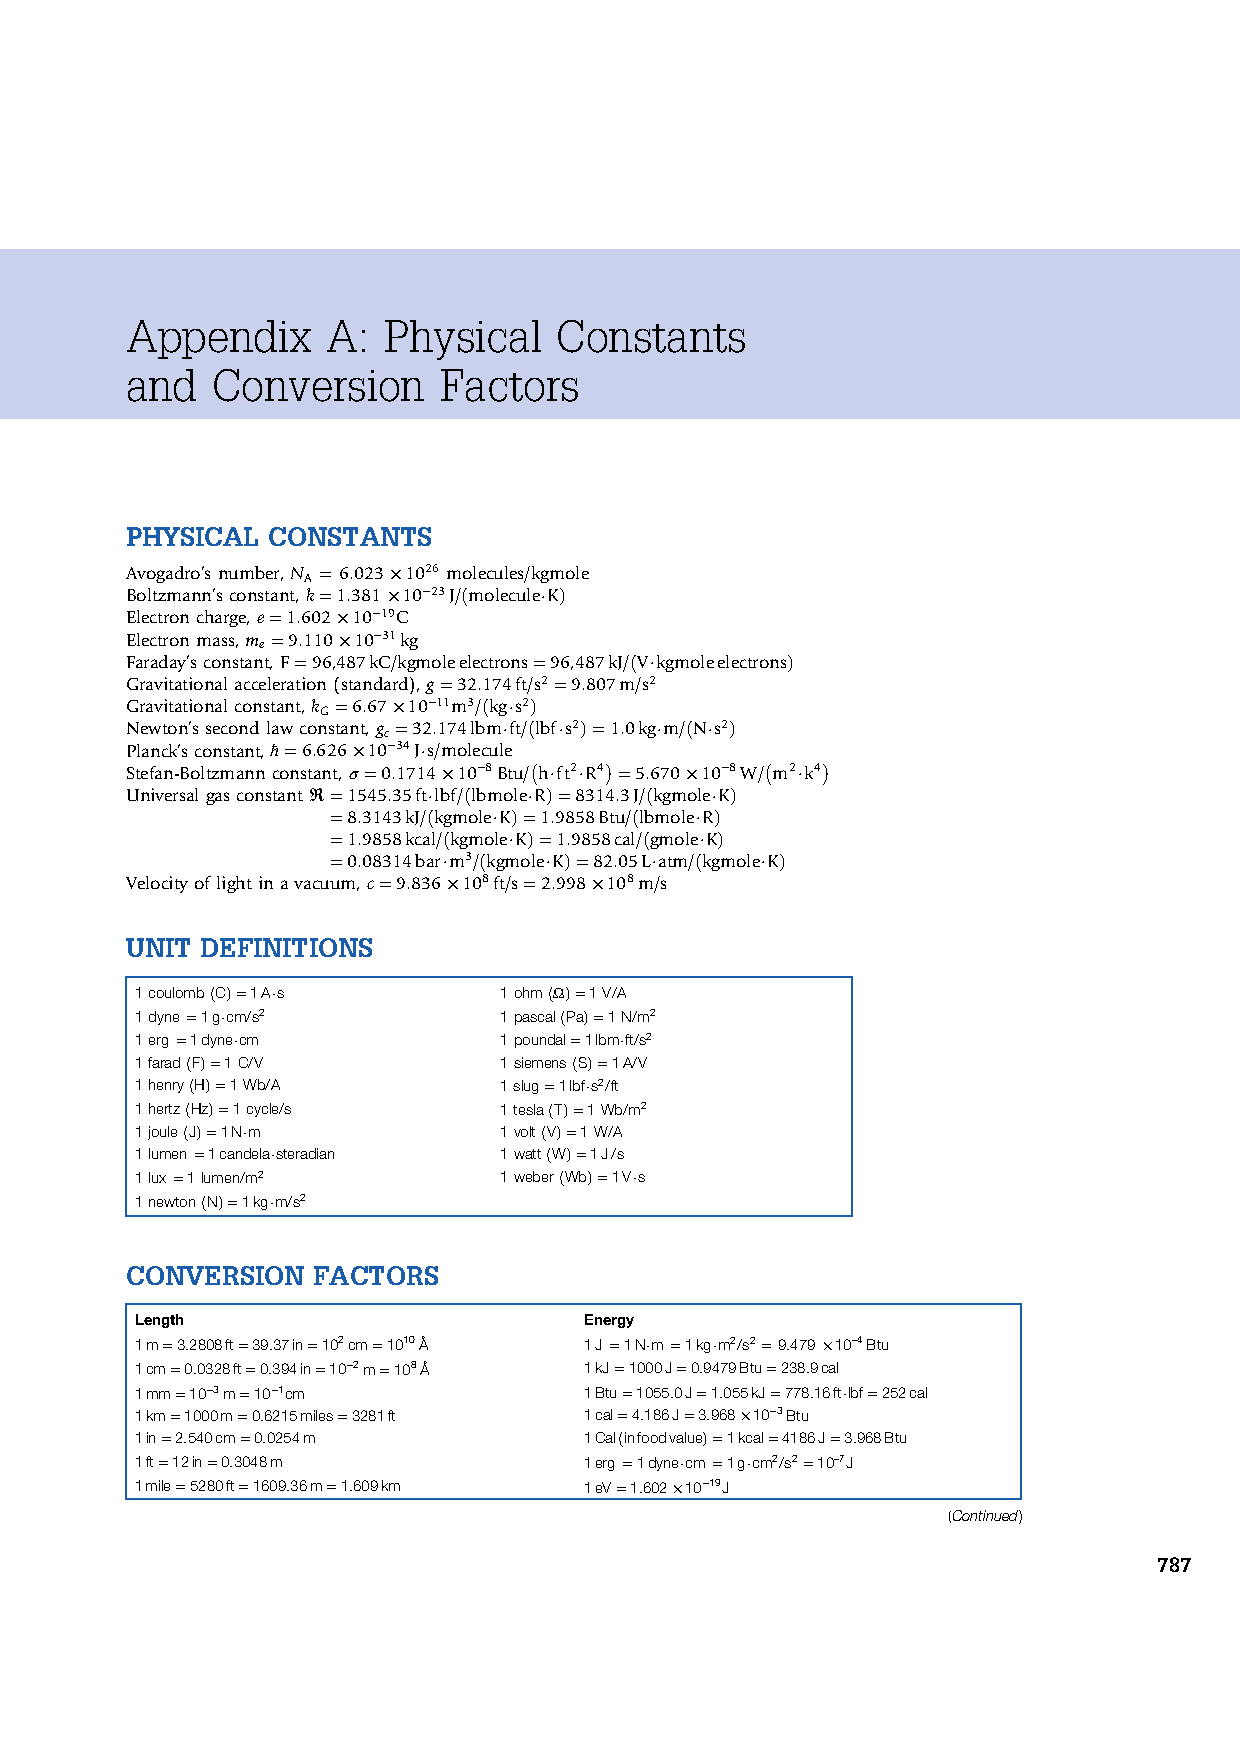
\includepdf[scale=1,pages=-,pagecommand={}, fitpaper]{./../Pics/ChemEng_UnitConv.pdf}

       
\chapter{Summary of Logarithms and Exponential Properties}
{\it This is not examinable} -- it is here so that you can see where some of the notations, operations and results of earlier sections come from. 

%%%% ETOC
\localtableofcontents

%%%
%%% EXPONENTS
%%%
\section{Exponents}
Assuming that $a$, $b$, $m$ and $n$ are real numbers, the following properties of exponents hold:
\begin{center}
  \begin{tabular}{||c l | c l ||}
    \hline\hline
     1 & $a^{m}a^{n} = a^{m+n}$ & 6 & $\frc{a^{m}}{a^{n}} = a^{m-n}$, $\forall a\neq 0$ \\
     2 & $\left(a^{m}\right)^{n} = a^{mn}$ & 7 &  $\left(ab\right)^{m} = a^{m}b^{m}$ \\
     3 & $\left(\frc{a}{b}\right)^{m} = \frc{a^{m}}{b^{m}}$, $\forall b\neq 0$ & 8 & $a^{-m}=\frc{1}{a^{m}}$, $\forall a\neq 0$ \\
     4 & $a^{1/n} = \sqrt[n]{a}$ & 9 & $a^{0} = 1$, $\forall a\neq 0$ \\
     5 & $a^{m/n} = \sqrt[n]{a^{m}} = \left(\sqrt[n]{a}\right)^{m}$ & & \\ 
    \hline\hline
  \end{tabular}
\end{center}


%%%
%%% LOGARITHMS
%%%
\section{Logarithms}
Let's define $y = \log_{a}x$ if ({\it and only if}) $x=a^{y}$, $\forall a>0$. Given the {\it Euler number}, $e$,
\begin{displaymath}
e = \sum\limits_{n=0}^{\infty}\frc{1}{n!}\sim 2.71828
\end{displaymath}
we can define $\ln x = \log_{e}{x}$, referred as the natural logarithm. The following properties of logarithms hold:
\begin{center}
  \begin{tabular}{||c l | c l||}
     \hline\hline
       1  & $\log_{a}b = \frc{\log_{10}{a}}{\log_{10}{b}}$ & 1' & $\log_{a}b = \frc{\ln{a}}{\ln{b}}$\\
     \hline
       2  & $\log_{a}{xy} = \log_{a}{x}+\log_{a}{y}$ & 2' &$\ln{xy} = \ln{x}+\ln{y}$  \\
     \hline
       3  & $\log_{a}{\frc{x}{y}} = \log_{a}{x}-\log_{a}{y}$ & 3' & $\ln{\frc{x}{y}} = \ln{x}-\ln{y}$ \\
     \hline
       4  & $\log_{a}{x^{y}} = y\cdot\log_{a}{x}$ & 4' & $\ln{x^{y}} = y\cdot\ln{x}$ \\
     \hline
       5  & $\log_{a}{a^{x}} = x$ & 5' & $\ln{e^{x}} = x$ \\
     \hline
       6  & $a^{\log_{a}{x}} = x$   & 6' & $e^{\ln{x}} = x$ \\
     \hline
       7  & $\log_{a}{a} = 1$, $\forall a>0$ & 7' & $\ln{e} = 1$ \\ 
     \hline
       8  & $\log_{a}1 = 0$, $\forall a > 0$ & 8' & $\ln{1} = 0$ \\
     \hline\hline
  \end{tabular}  
\end{center}
 
       
\chapter{Calculus' Background for Thermodynamics}\label{Appendix_Calculus}
{\it This is not examinable} -- it is here so that you can see where some of the notations, operations and results of earlier sections came from. Details of the contents of this Appendix can be found in \cite{Leithold_Book,Kallo_1955,Strang_Book} or in any {\it Calculus} text-book.
\bigskip


%%%% ETOC
\localtableofcontents

%%%
%%% SECTION
%%%
\section{Vector Calculus}

The operator {\it del} (or {\it nabla}),\index{{\it del} ($\nabla$) operator}\index{{\it nabla} ($\nabla$) operator}\index{$\nabla$}
\begin{displaymath}
  \nabla \equiv \left(\frc{\partial}{\partial x}, \frac{\partial}{\partial y}, \frac{\partial}{\partial z}\right)
\end{displaymath} 
is both a vector and a differential operator and can be used to define,
\begin{enumerate}
%
  \item Gradient: operates on a scalar field $\phi$, e.g., $T$, $\rho$, $\cdots$\index{Gradient}
     \begin{displaymath}
        \text{grad}\phi \equiv \nabla\phi \equiv \left(\frc{\partial\phi}{\partial x}, \frac{\partial\phi}{\partial y}, \frac{\partial\phi}{\partial z}\right)
     \end{displaymath}
%
  \item Divergence: operates on a vector field  $\theta = \left(\theta_{x}, \theta_{y}, \theta_{z}\right) $, e.g., velocity field.\index{Divergence}
     \begin{displaymath}
        \text{div}\theta \equiv \nabla\cdot\theta \equiv \frc{\partial\theta_{x}}{\partial x} + \frac{\partial\theta_{y}}{\partial y} + \frac{\partial\theta_{z}}{\partial z}
     \end{displaymath}
%
  \item Curl: operates on a vector field  $\theta = \left(\theta_{x}, \theta_{y}, \theta_{z}\right)$,\index{Curl}
     \begin{displaymath}
        \text{curl}\theta \equiv \nabla\times\theta \equiv \begin{pmatrix} i & j & k \\ \frc{\partial}{\partial x} & \frc{\partial}{\partial y} & \frc{\partial}{\partial z} \\ \theta_{x} & \theta_{y} & \theta_{z} \end{pmatrix}
     \end{displaymath}
%
   \item Laplacian: operates on a scalar field $\phi$,\index{Laplacian}
      \begin{displaymath}
         \text{div}\left(\text{grad}\phi\right) \equiv \nabla\cdot\nabla\phi \equiv \nabla^{2}\phi \equiv \frc{\partial^{2}\phi}{\partial x^{2}} + \frc{\partial^{2}\phi}{\partial y^{2}} + \frc{\partial^{2}\phi}{\partial z^{2}}
      \end{displaymath}
%
\end{enumerate}


%%%
%%% SECTION
%%%
\section{Some Basic Derivatives/Integration Operations}

\begin{center}
  \begin{tabular}{|| l l | l l ||}
    \hline\hline
       {\bf f(x)}  & {\bf f'(x)}  & {\bf f(x)}  & {\bf f'(x)}  \\
    \hline\hline
       $x^{n}$      &  $nx^{n-1}$   & $\ln{x}$    & $x^{-1}$      \\
       $e^{x}$      &  $e^{x}$      & $sin(x)$   & $cos(x)$     \\
       $cos(x)$    &  $-sin(x)$   & $tan(x)$    & $sec^{2}(x)$  \\
    \hline\hline
       {\bf f(x)}  &  {\bf $\int$f(x)dx} & {\bf f(x)}  &  {\bf $\int$f(x)dx} \\
    \hline\hline
       $e^{x}$      & $e^{x}+\mathcal{C}$& $x^{n}$ for $n\neq -1$ & $\frc{x^{n+1}}{n+1}+\mathcal{C}$ \\
                    &                  &                        & \\
       $1/x$ for $x\neq 0$& $\ln{|x|}+\mathcal{C}$ & $a^{x}$ for $a\neq 1$, $a>0$ & $\frc{a^{x}}{\ln{a}}+\mathcal{C}$\\
                   &                  &                         & \\
       $e^{ax}$ for $a\neq 0$  & $\frc{e^{ax}}{a}+\mathcal{C}$ & $cos(ax)$ for $a\neq0$ & $\frc{1}{a}sin(ax)+\mathcal{C}$\\
                   &                  &                        & \\
       $sin(ax)$ for $a\neq 0$ & $-\frc{1}{a}cos(ax)+\mathcal{C}$& & \\
    \hline\hline
  \end{tabular}
\end{center}

\begin{itemize}
%
  \item Derivative of a sum:
    \begin{displaymath}
       \frc{d}{dx}\left[f(x)+g(x)\right] = \frc{d}{dx}f(x) + \frc{d}{dx}g(x) = f'(x)+g'(x) 
    \end{displaymath}
%
  \item Derivative with a constant factor $c$:
    \begin{displaymath}
       \frc{d}{dx}\left[c f(x)\right] = c\frc{d}{dx}f(x) = cf'(x)
    \end{displaymath}
%
  \item Derivative of a product:
    \begin{displaymath}
       \frc{d}{dx}\left[f(x)g(x)\right] = f(x)g'(x) + f'(x)g(x)
    \end{displaymath}
%
  \item Derivative of a quotient:
    \begin{displaymath}
      \frc{d}{dx}\left[\frc{f(x)}{g(x)}\right] = \frc{g(x)f'(x)-f(x)g'(x)}{g^{2}(x)}
    \end{displaymath}
%
  \item Chain rule (or function of a function):
    \begin{displaymath}
      \frc{d}{dx}f\left[g(x)\right] = f'\left[g(x)\right]g'(x)
    \end{displaymath}
%
  \item Chain rule of a linear function:
    \begin{displaymath}
      \frc{d}{dx} \left[f(ax+b)\right] = a f'(ax+b)
    \end{displaymath}
%
  \item Integral of a function of a linear function:
    \begin{displaymath}
       \int\left[f'(ax+b)\right]dx = \frc{1}{a}f(ax+b) + \mathcal{C}
    \end{displaymath}
%
  \item Integral of a chain rule derivative:
    \begin{displaymath}
       \int\left\{f'\left[g(x)\right]g'(x)\right\}dx = f\left[g(x)\right] + \mathcal{C}
    \end{displaymath}
%
  \item Integral of a sum:
    \begin{displaymath}
      \int\left[f(x)+g(x)\right]dx = \int f(x)dx + \int g(x)dx
    \end{displaymath}
%
  \item Integral with a constant function:
    \begin{displaymath}
       \int c f(x)dx = c\int f(x)dx
    \end{displaymath}
%
  \item Integration by parts:
    \begin{displaymath}
       \int\left[f(x)g'(x)\right]dx = f(x)g(x) - \int\left[f'(x)g(x)\right]dx
    \end{displaymath}
%
  \item Definite integral (if $f'(x)$ is continuous at $a<x<b$):
    \begin{eqnarray}
       && \int\limits_{a}^{b}f(x)dx = - \int\limits_{b}^{a}f(x)dx \nonumber \\
       && \int\limits_{a}^{b}f'(x)dx = \left.f(x)\right|_{a}^{b} = \lim_{x\rightarrow b^{-}}f(x)-\lim_{x\rightarrow a^{+}}f(x)\nonumber
    \end{eqnarray}
%
  \item Substitution:
    \begin{eqnarray}
        \int f(x)dx = \int f(x(u))\frc{dx}{du}du && \text{(indefinite integral)} \nonumber \\
        \int\limits_{a}^{b} f(x) = \int\limits_{u(a)}^{u(b)}f(x(u))\frc{dx}{du}du  && \text{(definite integral)} \nonumber
    \end{eqnarray}
%
  \item Integration by parts:
    \begin{eqnarray}
       \int f(x)g'(x)dx = f(x)g(x) - \int f'(x)g(x) && \text{(indefinite integral)} \nonumber \\
       \int\limits_{a}^{b} f(x)g'(x)dx = \left.f(x)g(x)\right|_{a}^{b} - \int\limits_{a}^{b} f'(x)g(x) && \text{(definite integral)} \nonumber        
    \end{eqnarray}
%
\end{itemize}


%%%
%%% SECTION
%%%
\section{Partial Derivatives and Total Differentials}

%%% SUBSECTION
\subsection{Partial Derivatives:}\label{Appendix_Calculus:PartialDifferential}  Given a function $\phi\left(x_{1},x_{2},x_{3},\cdots,x_{n-1},x_{n}\right)$ of $n$ independent variables, the partial derivative of $\phi$ with respect to $x_{i}$, holding the other $n-1$ independent variables constant, is defined as,
  \begin{displaymath}
    \left(\frc{\partial\phi}{\partial x_{i}}\right)_{x_{j\neq i}} = \lim_{\Delta x_{i}\rightarrow 0}\left\{\frc{\phi\left(x_{1},x_{2},\cdots,x_{i}+\Delta x_{i},\cdots,x_{n}\right)-\phi\left(x_{1},x_{2},\cdots,x_{i},\cdots,x_{n}\right)}{\Delta x_{i}}\right\}
  \end{displaymath}

{\bf Example:} A pure fluid with ideal gas behaviour, the pressure can be expressed as a function of the number of mols ($n$), volume ($V$) and temperature ($T$),
  \begin{displaymath}
     P(n,V,T) = \frc{n R T}{V},
  \end{displaymath}
thus,
  \begin{displaymath}
     \left(\frc{\partial P}{\partial n}\right)_{V,T} = \frc{RT}{V}\hspace{1cm} \left(\frc{\partial P}{\partial V}\right)_{n,T} = -\frc{n R T}{V^{2}} \hspace{1cm} \left(\frc{\partial P}{\partial T}\right)_{n,V} = \frc{n R}{V}\d{T}
  \end{displaymath}


%%% SUBSECTION
\subsection{Total Differentials:}\label{Appendix_Calculus:TotalDifferential} Given a function $\phi\left(x_{1},x_{2},x_{3},\cdots,x_{n-1},x_{n}\right)$ of $n$ independent variables, the {\it total differential} of $\phi$, $d\phi$, is defined as
  \begin{eqnarray}
     d\phi &=& \sum\limits_{i=1}^{n}\left(\frc{\partial \phi}{\partial x_{i}}\right)_{x_{j\neq i}} d x_{i} \nonumber \\
     &=& \left(\frc{\partial\phi}{\partial x_{1}}\right)_{x_{2},\cdots,x_{n}} d x_{1} + \left(\frc{\partial\phi}{\partial x_{2}}\right)_{x_{1},x_{3},\cdots,x_{n}} dx_{2} + \cdots +  \left(\frc{\partial\phi}{\partial x_{n}}\right)_{x_{1},x_{2},\cdots,x_{n-1}} d x_{n} \nonumber 
  \end{eqnarray}
where $d x_{i}$ is an infinitesimal small increment in $x_{i}$.

\noindent
{\bf Example:} Infinitesimal changes in the ideal gas pressure are expressed as,
  \begin{eqnarray}
      d P &=& \left(\frc{\partial P}{\partial n}\right)_{V,T}\d{n} + \left(\frc{\partial P}{\partial V}\right)_{n,T}\d{V} + \left(\frc{\partial P}{\partial T}\right)_{n,V}\d{T} \nonumber \\
     &=& \frc{R T}{V} d n - \frc{n R T}{V^{2}} d V + \frc{n R}{V} d T. \nonumber 
  \end{eqnarray}

%%% SUBSECTION
\subsection{Properties of Partial Derivatives}\label{Appendix_Calculus:Properties}
  \begin{enumerate}[(i)]
%
     \item The order of differentiation in mixed second derivatives is immaterial, i.e.,
        \begin{displaymath}
           \left[\frc{\partial}{\partial y}\left(\frc{\partial\phi}{\partial x}\right)_{y}\right]_{x} = \left[\frc{\partial}{\partial x}\left(\frc{\partial\phi}{\partial y}\right)_{x}\right]_{y} \hspace{1cm}\Longleftrightarrow\hspace{1cm} \frc{\partial^{2}\phi}{\partial x\partial y} = \frc{\partial^{2}\phi}{\partial y\partial x}
        \end{displaymath}
%
     \item Cyclic rule:
        \begin{displaymath}
           \left(\frc{\partial\phi}{\partial x}\right)_{y}\left(\frc{\partial y}{\partial \phi}\right)_{x}\left(\frc{\partial x}{\partial y}\right)_{\phi} = -1
        \end{displaymath}
%
     \item Given $\phi(x,y)$ and $\varphi(x,y)$:
        \begin{enumerate}[(a)]
           \item $\left(\frc{\partial\phi}{\partial\varphi}\right)_{x} = \left(\frc{\partial\phi}{\partial y}\right)_{x}\left(\frc{\partial y}{\partial\varphi}\right)_{x}$  (chain rule);
           \item $\left(\frc{\partial\phi}{\partial x}\right)_{\varphi} = \left(\frc{\partial\phi}{\partial x}\right)_{y} + \left(\frc{\partial\phi}{\partial y}\right)_{x}\left(\frc{\partial y}{\partial x}\right)_{\varphi} $
        \end{enumerate}  
%
  \end{enumerate}

%%%
%%% SECTION
%%%
\section{The Mean Value Theorem and l'H\^opital's Rule}\label{Appendix:lHopital}

\begin{theorem}[Mean value]\index{Mean value theorem}\label{Appendix:MeanValueTheorem}
Suppose $f(x)$ is continuous in the closed interval $a\leq x\leq b$ and has derivatives everywhere in the open interval $a<x<b$. Then,
     \begin{equation}
       \frc{f(a)-f(b)}{b-a} = f'(c)\;\;\;\text{ at some point } a<c<b.
     \end{equation}
\end{theorem}

\begin{theorem}[Rolle's theorem, i.e., extrema of a function]\index{Mean value theorem ! Rolle's theorem}
   Suppose $f(a) = f(b) = 0$ (zero at endpoints). Then $f'(c) = 0$ at some point within $a<c<b$.
\end{theorem}

\begin{theorem}[l'H\^opital rule]\index{Mean value theorem ! L'H\^opital rule}\index{L'H\^opital rule}
   Suppose $f(x)$ and $g(x)$ are differentiable and $g'(x)\neq 0$ near a point $a$ (except possibly at $a$). Suppose that
    \begin{displaymath}
      \lim_{x\rightarrow a} f(x) = 0 \;\;\text{ and }\;\; \lim_{x\rightarrow a} g(x) = 0,
    \end{displaymath}
or that
    \begin{displaymath}
      \lim_{x\rightarrow a} f(x) = \pm\infty \;\;\text{ and }\;\; \lim_{x\rightarrow a} g(x) = \pm\infty,
    \end{displaymath}
$\left(\text{i.e., an indeterminate quotient, }\frc{0}{0} \text{ or }\frc{\infty}{\infty}\right)$. Then
    \begin{equation}
        \lim_{x\rightarrow a}\frc{f(x)}{g(x)} = \lim_{x\rightarrow a}\frc{f'(x)}{g'(x)},
    \end{equation}
if the limit on the right side exists (or is $\infty$ or $-\infty$).
%both approach zero as $x\rightarrow a$. Then $\frc{f(x)}{g(x)}$ approaches the same limit as $\frc{f'(x)}{g'(x)}$, if this second limit exists,
%    \begin{equation}
%        \lim_{x\rightarrow a}\frc{f(x)}{g(x)} = \lim_{x\rightarrow a}\frc{f'(x)}{g'(x)}.
%    \end{equation}
%   This limit often is $\frc{f'(a)}{g'(a)}$.
    \begin{list}{\bf Example \arabic{qcounter}:~}{\usecounter{qcounter}}
%       
       \item Find $\lim\limits_{x\rightarrow\infty} \frc{5x-2}{7x+3}$.
           \begin{eqnarray}
              \lim_{x\rightarrow\infty}\frc{5x-2}{7x+3} &=& \frc{\infty}{\infty} \nonumber \\
                                                   &=& \lim_{x\rightarrow\infty}\frc{\left[5x-2\right]'}{\left[7x+3\right]'} = \lim_{x\rightarrow\infty} \frc{5}{7} = \frc{5}{7}\nonumber
           \end{eqnarray}
%
      \item Find $\lim\limits_{x\rightarrow -2}\frc{x+2}{\ln{(x+3)}}$. 
           \begin{eqnarray}
              \lim_{x\rightarrow -2}\frc{x+2}{\ln{(x+3)}} &=& \frc{0}{0} \nonumber \\                                                   &=& \lim_{x\rightarrow -2}\frc{\left[x+2\right]'}{\left[\ln{(x+3)}\right]} = \lim_{x\rightarrow -2} \frc{1}{\frc{1}{x+3}} = \lim_{x\rightarrow -2} \left(x+3\right) = 1 \nonumber
           \end{eqnarray}
         
%
    \end{list}


\end{theorem}

%%%
%%% SECTION
%%%
\section{Line Integrals}\index{Line integral}

%%%
\subsection{Exact and Inexact Differential}\index{Line integral!Exact differential}\index{Line integral!Inexact differential}
Consider that $\mathbf{\Psi}$ is a function of the independent variables $x_{j}$ (with $j=1,2,\cdots,n$),  $\Psi_{i}=\Psi_{i}\left(x_{1},x_{2},\cdots,x_{n}\right)$. An infinitesimal quantity,
   \begin{displaymath}
      dz = \sum\limits_{i=1}^{n} \Psi_{i}\left(x_{1},x_{2},\cdots,x_{n}\right) d x_{i} =  \Psi_{1} d x_{1} + \Psi_{2} d x_{2} +\cdots + \Psi_{n} d x_{n},
   \end{displaymath}
is called {\it linear differential}\index{Linear differential}. If we focus on a two-dimensional problem, i.e., $\mathbf{\Psi}=\left\{M(x,y),N(x,y)\right\}$,
   \begin{equation}
      dz = M d x + N d y\label{Appendix_Calculus:Eqn:ExactLinearDifferential}
   \end{equation}

\medskip
Equation~\ref{Appendix_Calculus:Eqn:ExactLinearDifferential} is an {\it exact differential}\index{Exact differential} if, and only if, there is a function of $x$ and $y$, $\Phi(x,y)$, such that $d \Phi= d z$ for all values of $x$ and $y$. This is equivalent to
   \begin{displaymath}
        \Partial[M]{y}{x} = \Partial[N]{x}{y}.
   \end{displaymath}
The equation
   \begin{equation}
      dw = M^{\prime} d x + N^{\prime} d y,\label{Appendix_Calculus:Eqn:InexactLinearDifferential}
   \end{equation}
 is an {\it inexact differential}\index{Inexact differential} if, and only if, there is no function $\Phi(x,y)$, such that $d \Phi = d w$ for all values of $x$ and $y$, thus,
   \begin{displaymath}
        \Partial[M^{\prime}]{y}{x} \neq \Partial[N^{\prime}]{x}{y}.
   \end{displaymath}

%%%
\subsection{Fundamental Theorem for Line Integrals}\index{Line integral!Fundamental theorem}\label{Appendix_Calculus:Section:LineIntegral}

\begin{theorem}
   If {\bf F} is a gradient or conservative vector field, i.e., $\mathbf{F}=\mathbf{\nabla}f(x,y)=\langle f_{x}, f_{y}\rangle$ for a {\it potential function} $f$ for the field, and $\mathcal{C}$ is a curve with endpoints $P_{0}=\left(x_{0},y_{0}\right)$ and $P_{1}=\left(x_{1},y_{1}\right)$,
      \begin{eqnarray}
         \int\limits_{\mathcal{C}}\mathbf{F}\cdot d\mathbf{r} &=& \int\limits_{\mathcal{C}}\mathbf{\nabla}f d \mathbf{r} = \left.f(x,y)\right|_{P_{0}}^{P_{1}}\\
                                                           &=& f\left(P_{1}\right)-f\left(P_{0}\right) = f\left(x_{1},y_{1}\right) - f\left(x_{0},y_{0}\right)\nonumber.
      \end{eqnarray}
\end{theorem} 
That is, for gradient fields the line integral is independent of the path taken, i.e., it depends only on the endpoints of $\mathcal{C}$. We call such a line integral {\it path independent}.
\medskip

The line integral of a vector field over a {\it simple} (i.e., non-intersecting) {\it closed} (i.e., no endpoints) curve $\mathcal{C}$ is denoted as,\index{Line integral}
        \begin{equation}
           \oint_{\mathcal{C}}\mathbf{F}\cdot d \mathbf{r} = 0,
        \end{equation}
i.e., the line integral around all closed paths is 0 $\leftrightarrow$ -- {\it path independence}.
   
       
\chapter{Introduction to Numerical Methods relevant to Thermodynamics}\label{Appendix_NumMethods}


%%%% ETOC
\localtableofcontents

{\it This is not examinable} -- it is here so that you can see where some of the notations, operations and results of earlier sections came from. Details of the contents of this Appendix can be found in \cite{Atkinson_Book_Newton,Atkinson_Book_Interpolation,NumericalRecipes_Interpolation,NumericalRecipes_Newton} or in any text-book of {\it Mathematical or Numerical Methods} for engineering.

%%%
%%% SECTION
%%%
\section{Linear Interpolation}\label{LinearInterpolation}\index{Linear interpolation}

Given a continuous and unknown function $f(x)$, defined at a set of points  $x_{1} < \cdots < x_{i} < \cdots < x_{N}$. Interpolation is the process of determining a polynomial expression to calculate the pair $\left[x_{k}, f\left(x_{k}\right)\right]$ based on neighbours discrete coordinates $\left\{\left[x_{1},f\left(x_{1}\right)\right], \cdots, \left[x_{N},f\left(x_{N}\right)\right]\right\}$. 

Consider a set of discrete data points,
  \begin{center}
    \begin{tabular}{c | c }
        $\mathbf{x}$   & $\mathbf{f\left(x_{i}\right)}$ \\
        \hline
           $x_{1}$ &  $f\left(x_{1}\right)$ \\
           $x_{2}$ &  $f\left(x_{2}\right)$ \\
           $x_{3}$ &  $f\left(x_{3}\right)$ \\
           $x_{4}$ &  $f\left(x_{4}\right)$ \\
    \end{tabular}
  \end{center}
that are a subset of a continuous and smooth function $y=f(x)$ (Fig.~\ref{Appendix:Fig:Interpolation}). Polynomials of order $n\ge 1$ can be generated to represent this function. High-order polynomials can more accurately fit the discrete coordinatess than low-order polynomials. In Fig.~\ref{Appendix:Fig:Interpolation}, let's assume the discrete pairs 
  \begin{displaymath}
     \left\{\left[x_{1},f\left(x_{1}\right)\right], \left[x_{2},f\left(x_{2}\right)\right],\left[x_{3},f\left(x_{3}\right)\right], \left[x_{4},f\left(x_{4}\right)\right]\right\}
  \end{displaymath}
are known, and one wants to determine the value of the function $f$ at $x_{2} < x_{k} < x_{3}$. If the interval $\Delta x= x_{3}-x_{2}$ is sufficiently small, a linear function can be used to fit these coordinates,
   \begin{displaymath}
       f\left(x_{k}\right) = f\left(x_{2}\right) + m\left(x_{k}-x_{2}\right),%\label{LinearInterpolation:Eqn1}
   \end{displaymath}
where 
   \begin{displaymath}
      m = \frc{f\left(x_{3}\right)-f\left(x_{2}\right)}{x_{3}-x_{2}}.
   \end{displaymath}
If $m$ is replaced in the previous equation, %Eqn.~\ref{LinearInterpolation:Eqn1},
   \begin{displaymath}
       f\left(x_{k}\right) = \frc{f\left(x_{2}\right)\left(x_{3}-x_{k}\right) + f\left(x_{3}\right)\left(x_{k}-x_{2}\right)}{x_{3}-x_{2}}.
   \end{displaymath}
   
   \begin{shaded}
      Or for a general case with $x_{a} < x_{k} < x_{b}$,
        \begin{equation}\label{LinearInterpolation:Eqn1}
            f\left(x_{k}\right) = \frc{f\left(x_{a}\right)\left(x_{b}-x_{k}\right) + f\left(x_{b}\right)\left(x_{k}-x_{a}\right)}{x_{b}-x_{a}}.
        \end{equation}
   \end{shaded}

%%% Figure
     \begin{figure}[h]\label{Appendix:Fig:Interpolation}%
        \begin{center}
          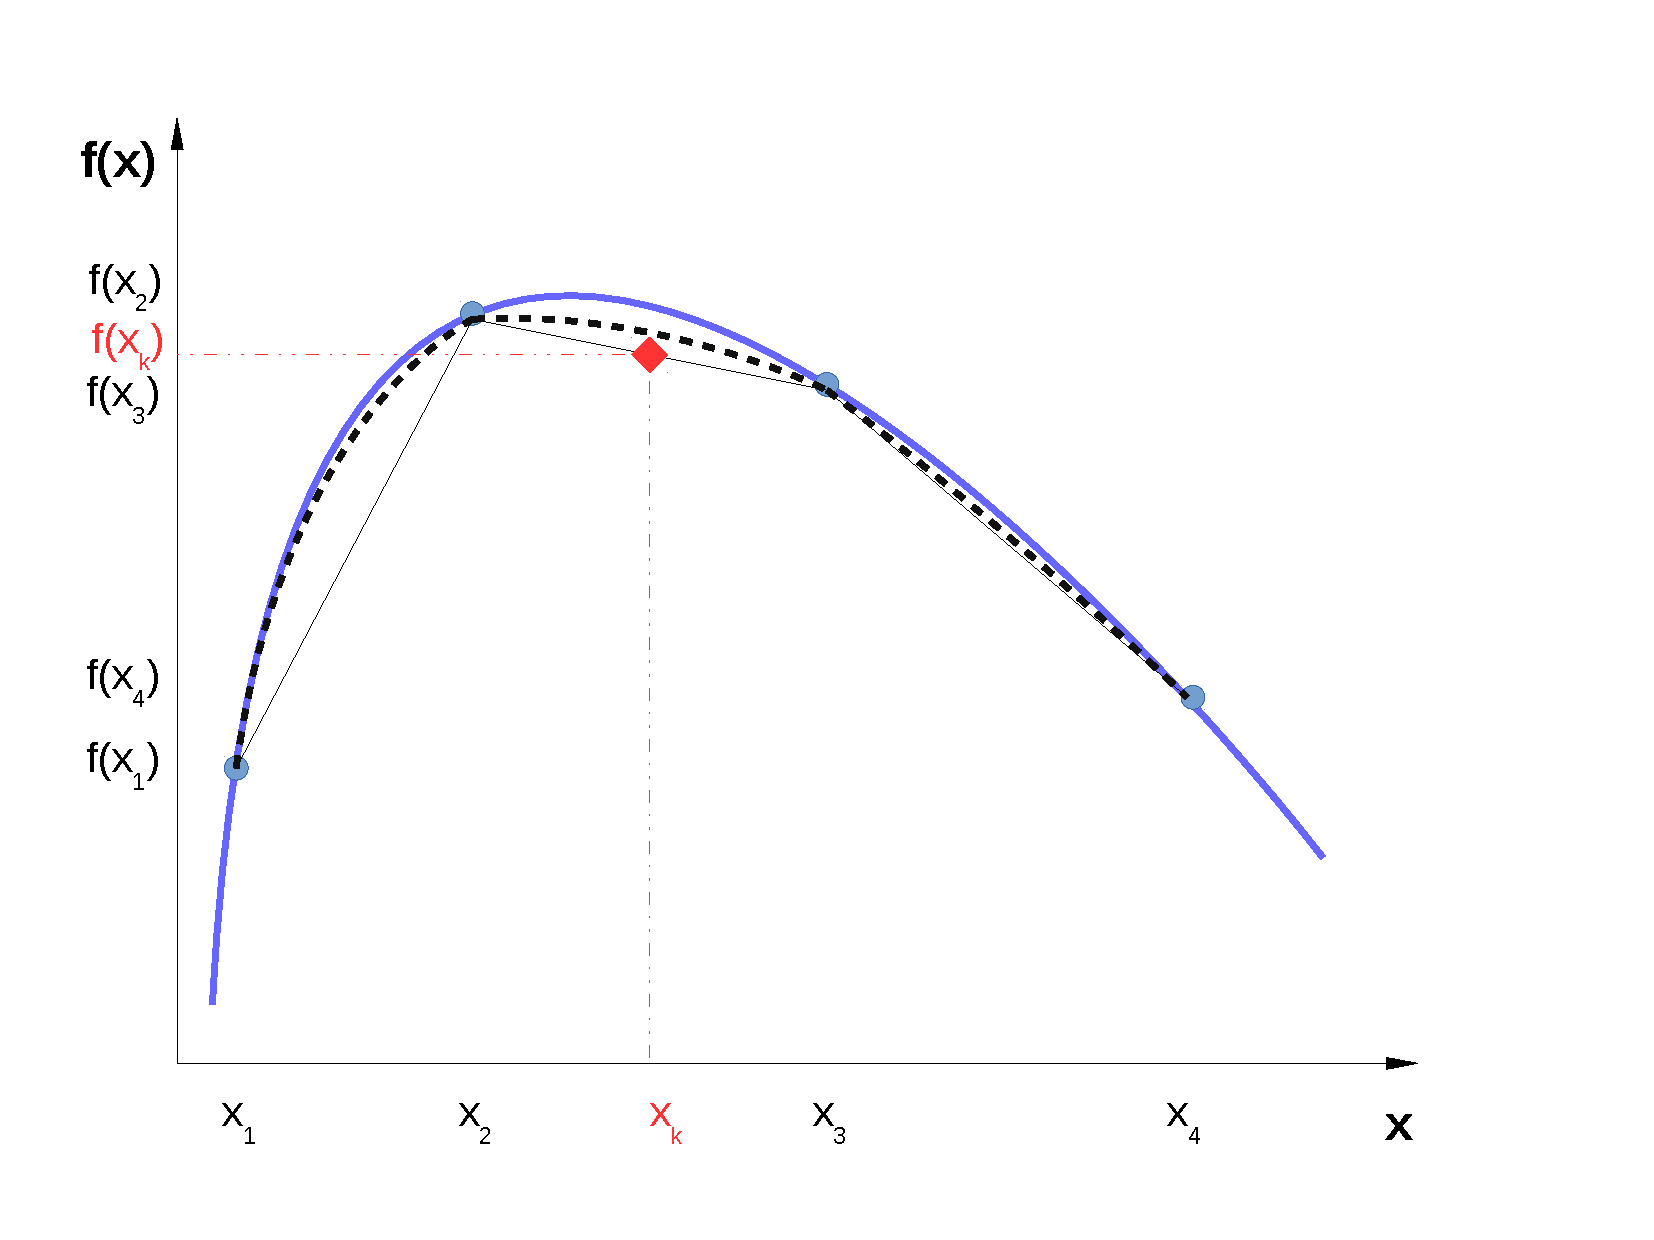
\includegraphics[width=\columnwidth,clip]{./../Pics/Interpolation}
           \caption{Smooth function $f(x)$ (solid blue line) may be more accurately interpolated by a high-order polynomial (black dotted line) than by a low-order polynomial (solid black line).} 
        \end{center}
      \end{figure}

   % Example
   \begin{MyExample}{\begin{center}{\bf Example}\end{center}}
      \begin{example}
         Given a table of values for $f(x)=\tan{x}$ for a few values of $x$,
            \begin{center}
               \begin{tabular}{c | c c c c}
                   $x$        & 1.00   & 1.10   & 1.20   & 1.30   \\
                   \hline
                   $\tan{x}$  & 1.5574 & 1.9648 & 2.5722 & 3.6021 \\
               \end{tabular}
            \end{center}
            Estimate $\tan{(1.15)}$ and $\tan{(1.23)}$.
     \end{example}

% SOLUTION
       \noindent{\bf Solution:} For $\left(x_{a}=1.10\right) < \left(x_{k}=1.15\right) < \left(x_{b}=1.20\right)$,
               \begin{eqnarray}
                  f\left(x_{k}\right) &=& \frc{f\left(x_{a}\right)\left(x_{b}-x_{k}\right) + f\left(x_{b}\right)\left(x_{k}-x_{a}\right)}{x_{b}-x_{a}} \nonumber \\
                                     &=& \frc{1.9648\times(1.20-1.15) + 2.5722\times(1.15-1.10)}{1.20-1.10} = 2.2685 \nonumber
               \end{eqnarray}

For  $\left(x_{a}=1.20\right) < \left(x_{k}=1.23\right) < \left(x_{b}=1.30\right)$,
               \begin{eqnarray}
                  f\left(x_{k}\right) &=& \frc{f\left(x_{a}\right)\left(x_{b}-x_{k}\right) + f\left(x_{b}\right)\left(x_{k}-x_{a}\right)}{x_{b}-x_{a}} \nonumber \\
                                     &=& \frc{2.5722\times(1.30-1.23) + 3.6021\times(1.23-1.20)}{1.30-1.20} = 2.8812 \nonumber
               \end{eqnarray}
   \end{MyExample}

   % Example
   \begin{MyExample}{\begin{center}{\bf Example}\end{center}}
      \begin{example}
         Calculate specific volume $\left(v, \text{in m}^{3}\text{.kg}^{-1}\right)$, internal energy $\left(u, \text{in kJ.kg}^{-1}\right)$ and entropy $\left(s, \text{in kJ.(kg.K)}^{-1}\right)$ of saturated water vapour at 133.45$^{\circ}$C.
     \end{example}

% SOLUTION
       \noindent{\bf Solution:} From Appendix~\ref{Appendix:Saturated_SH_Tables} (Table A-2), for $T_{a}(=130.0) < T_{k} (= 133.45) < T_{b} (=140.0)^{\circ}C$, thus:
               \begin{eqnarray}
                  v\left(T_{k}\right) &=& \frc{v\left(T_{a}\right)\left(T_{b}-T_{k}\right) + v\left(T_{b}\right)\left(T_{k}-T_{a}\right)}{T_{b}-T_{a}} \nonumber \\
                                     &=& \frc{0.6685\times(140.0-133.45) + 0.5089\times(133.45-130.0)}{140.0-130.0} = 0.6134 \text{ m}^{3}\text{.kg}^{-1}\nonumber \\
                                     && \nonumber \\
                  u\left(T_{k}\right) &=& \frc{u\left(T_{a}\right)\left(T_{b}-T_{k}\right) + u\left(T_{b}\right)\left(T_{k}-T_{a}\right)}{T_{b}-T_{a}} \nonumber \\
                                     &=& \frc{2539.9\times(140.0-133.45) + 2550.0\times(133.45-130.0)}{140.0-130.0} = 2543.39 \text{ kJ.kg}^{-1}\nonumber \\
                                     && \nonumber \\
                  s\left(T_{k}\right) &=& \frc{s\left(T_{a}\right)\left(T_{b}-T_{k}\right) + s\left(T_{b}\right)\left(T_{k}-T_{a}\right)}{T_{b}-T_{a}} \nonumber \\
                                     &=& \frc{7.0269\times(140.0-133.45) + 6.9299\times(133.45-130.0)}{140.0-130.0} = 6.9934 \text{ kJ.}\left(\text{kg.K}\right)^{-1}\nonumber 
               \end{eqnarray}
   \end{MyExample}


%%%
%%% SECTION
%%%
\section{Root-Finder Methods}\label{Section:RootFinderMethods}\index{Root-Finder Methods}

%%% SUBSECTION
\subsection{Motivation}
Given a smooth, {\it continuous} and {\it fully differentiable} function 
  \begin{displaymath}
     y = f(x) \hspace{3cm} \text{ with } x\in\mathbb{R}.
  \end{displaymath}
We aim to find the root $x=\psi$ of the function 
  \begin{displaymath}
     f(x) = 0.
  \end{displaymath}
The first step is to estimate $x_{0}$ that results in $f\left(x_{0}\right)\neq 0$ and may lead to a new estimate $x_{1}$. The procedure is repeated until $f\left(x_{n}\right)\rightarrow 0$ (\ie $x_{n}\approx\psi$), where $n$ is the number of repetitions (or {\it iterations}). There are several methods designed to solve non-linear equations, i.e., find the rrot of the function, here we will focus on the most popular {\it Newton-Raphson} method that combines simplicity and power.


%%% SUBSECTION
\subsection{Newton-Raphson Iterative Method}\label{Section:RootFinderMethods:NewtonRaphson}\index{Root-Finder Methods!Newton-Raphson method}
Let's assume that $x_{0}$ is a good estimate of the root$\psi$ and $\psi = x_{0} + h$. Since the root of the function $f(x)$ is $\psi$ and $h = \psi 0 x_{0}$, $h$ represents the distance between the initial estimate (or guess) and the root. Assuming $h$ is very (or {\it infinitesimal}) small, we can linearly approximate the function,
   \begin{displaymath}
        f\left(\psi\right) = 0 = f\left(x_{0}+h\right) \approx f\left(x_{0}\right) + h f'\left(x_{0}\right).
   \end{displaymath}
Therefore, except if $f'\left(x_{0}\right)$ is close to $0$, 
   \begin{displaymath}
        h \approx -\frc{f\left(x_{0}\right)}{f'\left(x_{0}\right)} \hspace{.3cm} \Longrightarrow \hspace{.3cm} \psi = x_{0} + h \approx x_{0} -\frc{f\left(x_{0}\right)}{f'\left(x_{0}\right)}.
   \end{displaymath}
%%% Figure
     \begin{figure}[h]\label{Appendix:Fig:NewtonRaphson}%
        \begin{center}
         \vbox{
           \hbox{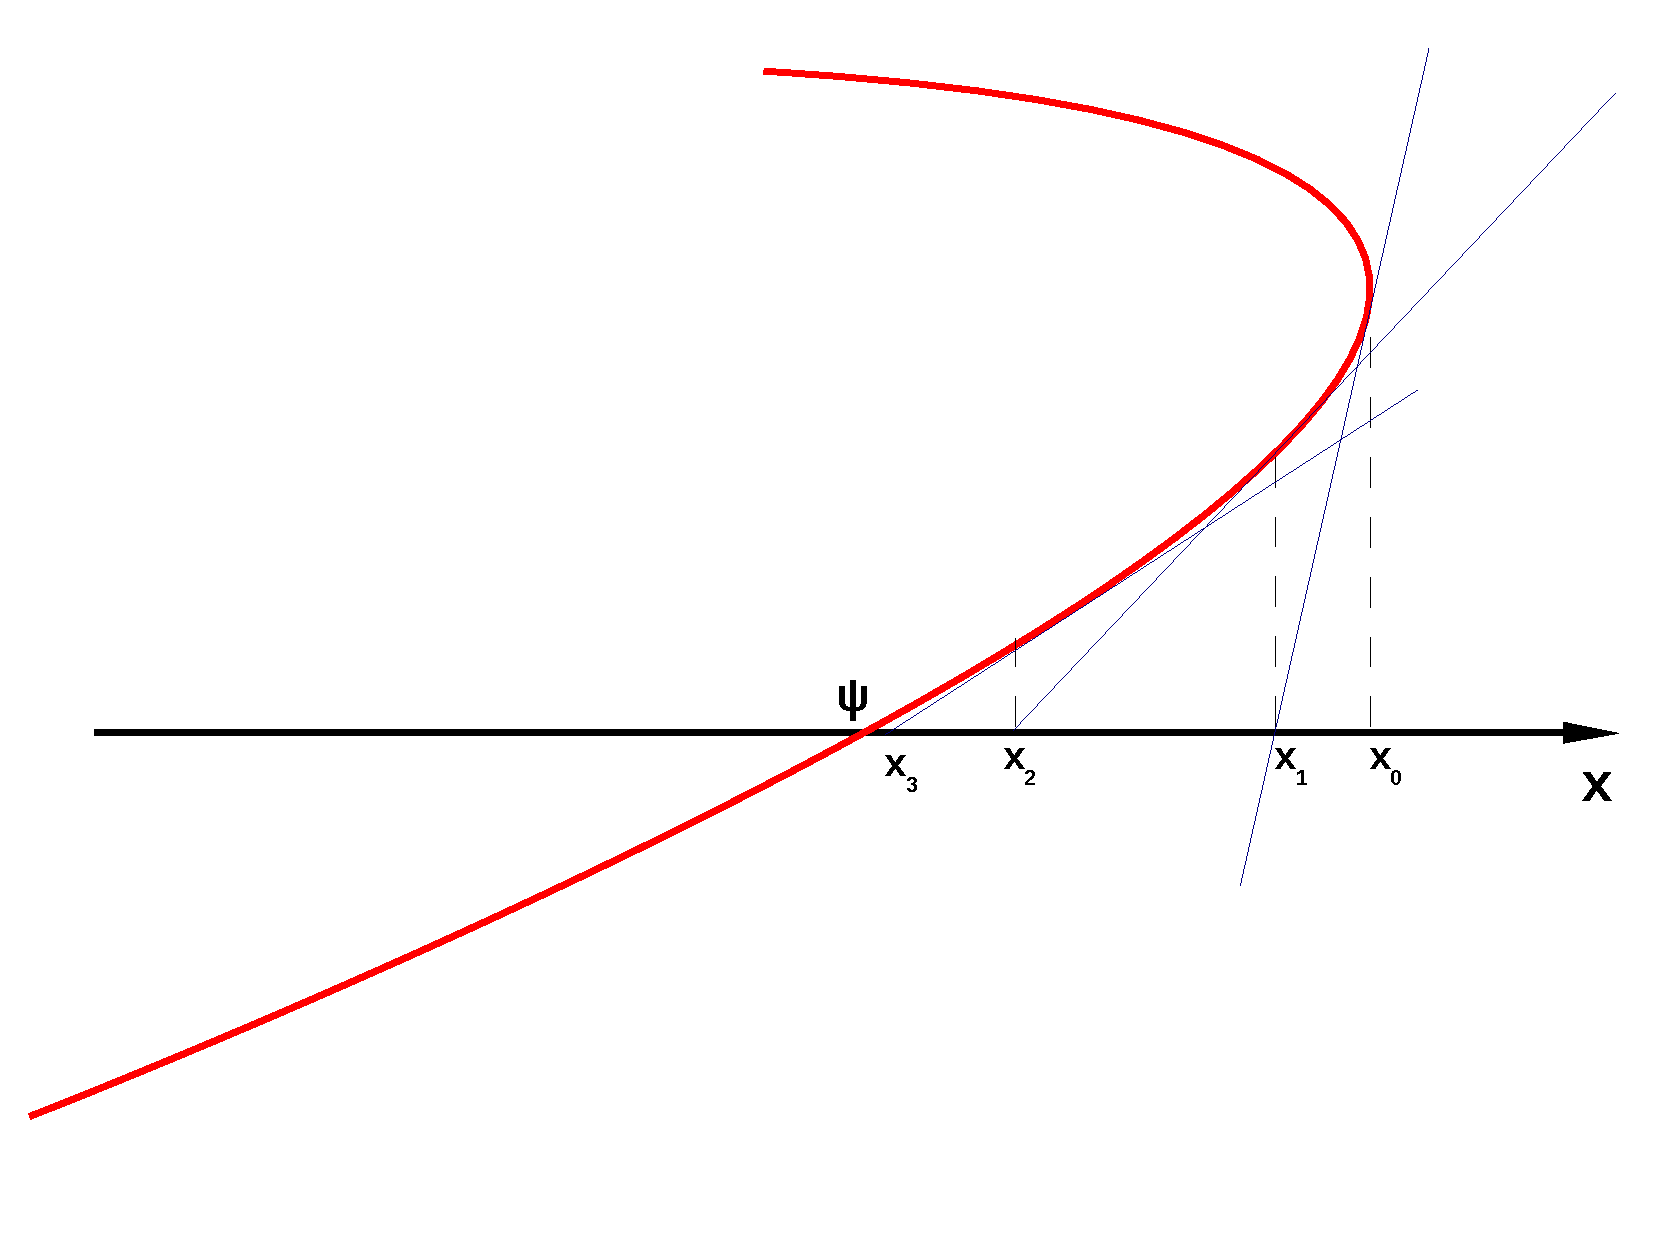
\includegraphics[width=\columnwidth,height=10cm]{./../Pics/NewtonRaphson2}}
           \hbox{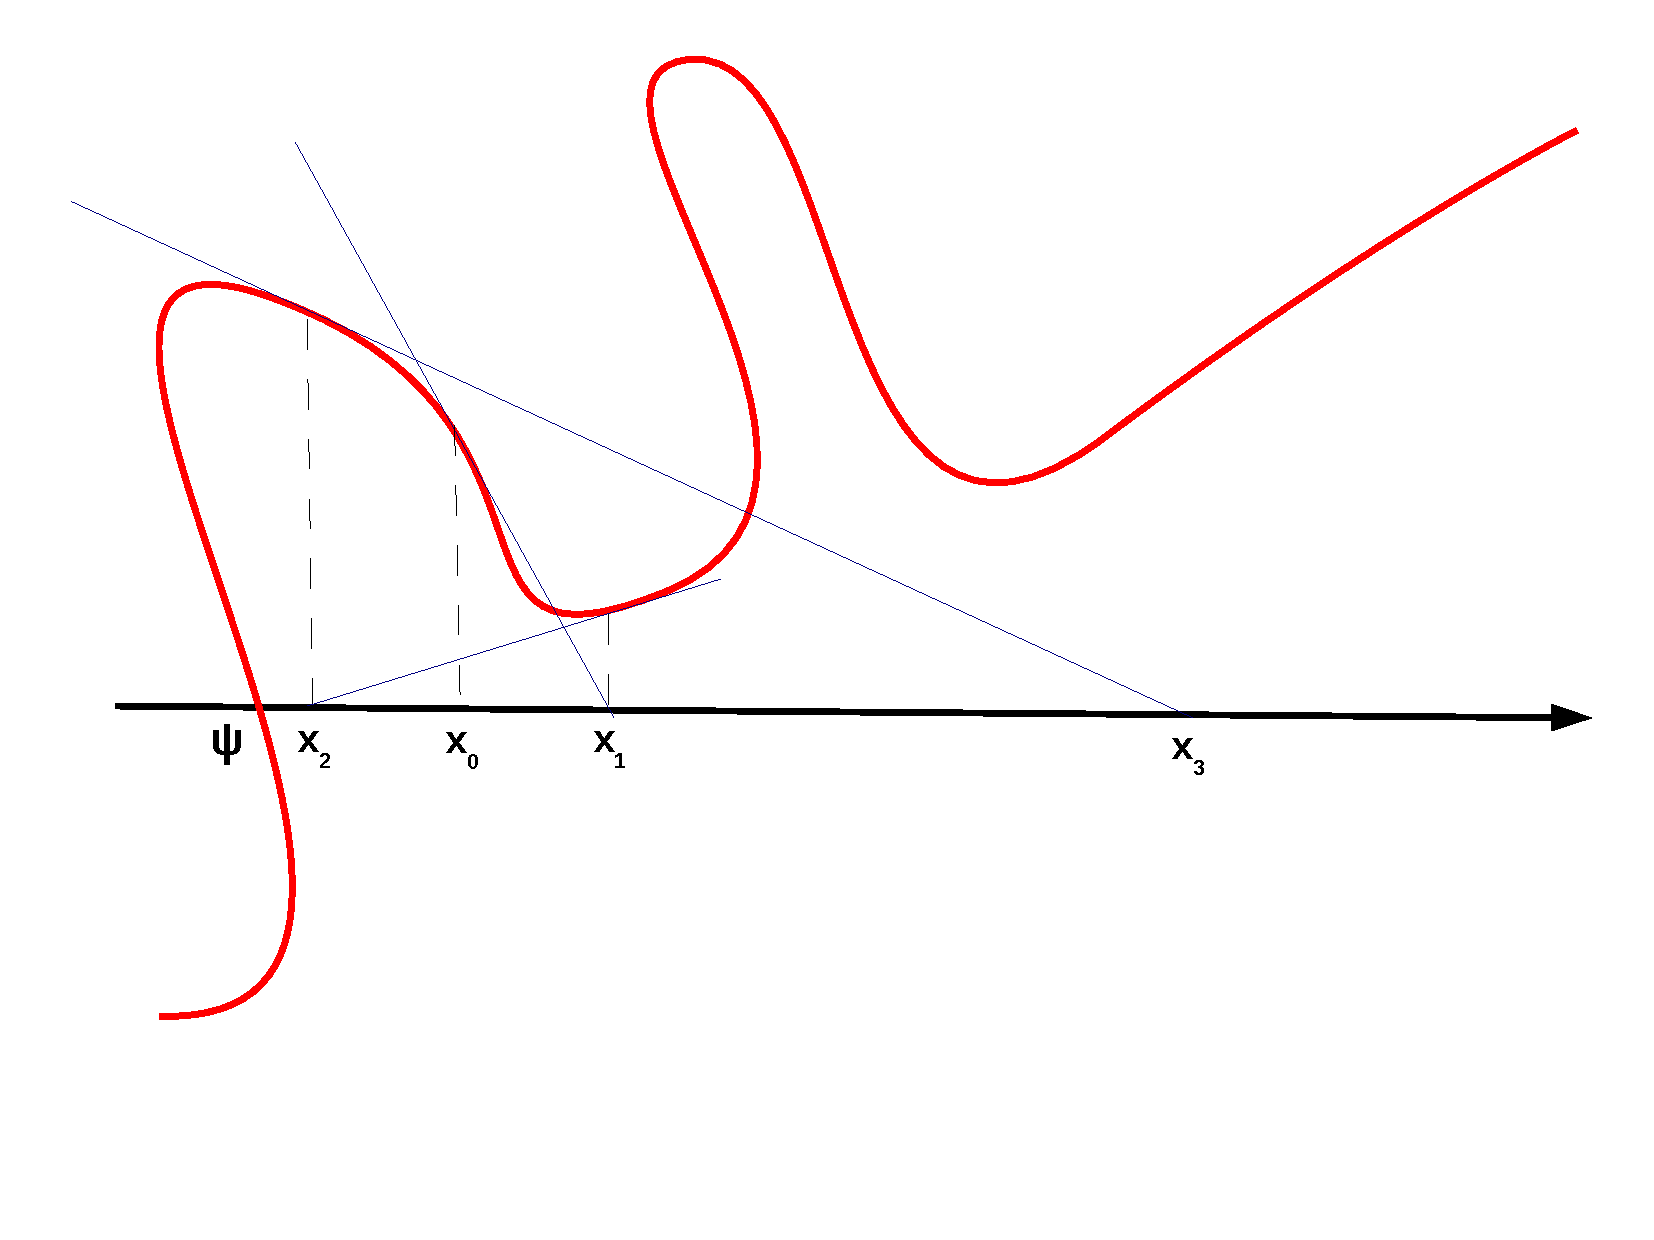
\includegraphics[width=\columnwidth,height=10cm]{./../Pics/NewtonRaphson3}}}
           \vspace{-1cm}
           \caption{Graphic representation of the Newton-Raphson iterative method: (top) solution of the smooth and continuous function $f(x)$ (solid red line) is approximated from the initial estimate $x_{0}$ to the final solution $x=\psi$; (bottom) initial estimate $x_{0}$ is far away from the root $\psi$ and the solution may diverge. Blue solid lines are tangent of the function at $x_{i}$.} 
        \end{center}
      \end{figure}
%
This expression represents an improvement of the original estimate, i.e.,  
   \begin{displaymath}
        x_{1} = x_{0} -\frc{f\left(x_{0}\right)}{f'\left(x_{0}\right)}.
   \end{displaymath}
The next estimate, $x_{2}$, is obtained from $x_{1}$, 
   \begin{displaymath}
        x_{2} = x_{1} -\frc{f\left(x_{1}\right)}{f'\left(x_{1}\right)}.
   \end{displaymath}

   \begin{shaded}
      We can generalise this expression for the $n-${\it th iteration},
         \begin{equation}
            x_{n+1} = x_{n} -\frc{f\left(x_{n}\right)}{f'\left(x_{n}\right)}.\label{NewtonRaphson:Eqn1}
         \end{equation}
   \end{shaded}

Figure~\ref{Appendix:Fig:NewtonRaphson}(a) shows a geometrical representation of the Newton-Raphson iterative method, where $m=f(x)$ is the tangent (blue) line at the coordinate pair $\left[x_{0},f\left(x_{0}\right)\right]$,
   \begin{displaymath}
     m = f\left(x_{0}\right) + \left(x-x_{0}\right)f'\left(x_{0}\right).
   \end{displaymath}
Let $x_{1}$ be the {\it x-intercept} of the tangent line, therefore
   \begin{displaymath}
     x_{1} = x_{0} - \frc{f\left(x_{0}\right)}{f'\left(x_{0}\right)}
   \end{displaymath}
The tangent line is a geometrical representation of the Newton-Raphson iterative method, Eqn.~\ref{NewtonRaphson:Eqn1}, as the estimates gradually tend to the root $\psi$ of the function. As it can be seen in the Fig.~\ref{Appendix:Fig:NewtonRaphson}(b), if the initial estimate $x_{0}$ is not close enough of the root $\psi$, the solution may not {\it converge}. In fact, the Newton-Raphson iterative method works most of the time if the initial estimate is {\it good enough}.

 From the {\it mean value theorem} (Theorem~\ref{Appendix:MeanValueTheorem}), let the function $f(x)$ be such that, 
   \begin{enumerate}[(a)]
      \item it is continuously differentiable in some open interval containing the solution $x=\psi$;
      \item $\left|f'(\psi)\right| < 1$.
   \end{enumerate}
Then there is a number $\epsilon > 0$ such that the iteration $x_{k+1}=f\left(x_{k}\right)$ {\it converges} whenever $x_{0}$ is chosen in $\left|x_{0}-\psi\right|\leq\epsilon$.

For bounded $x\in\mathbb{R}$ (\ie contained in the interval $a\leq x \leq b$), if $f''(x)$ exists and is continuous on $[a,b]$ and $\psi$ is a root of $f(x)$, that is, $f(\psi)=0$ and $f'(\psi)\neq0$. Thus for a function $g(x)$
    \begin{displaymath}
        g(x) = x - \frc{f(x)}{f'(x)}
    \end{displaymath}
with
    \begin{displaymath}
        g'(x) = 1 - \frc{[f'(x)]^{2} - f(x)f''(x)}{[f'(x)]^{2}} = \frc{f(x)f''(x)}{[f'(x)]^{2}},
    \end{displaymath}
and
    \begin{displaymath}
        g'(\psi) = \frc{f(\psi)f''(\psi)}{[f'(\psi)]^{2}}=0, \text{ since } f(\psi) = 0 \text{ and } f'(\psi) \neq 0
    \end{displaymath}
As $g'(x)$ is continuous, this means that there is a small neighbourhood around the root $x=\psi$ such that for all points $x$ in that neighbourhood, $\left|g'(x)\right|<1$.  Therefore, if $g(x)$ is chosen as above and the initial estimate $x_{0}$ is chosen {\it sufficiently close to the root} $x=\psi$, then the Newton-Raphson method is {\it guaranteed to converge}. 

Algorithm~\ref{Algorithm:NewtonRaphson} highlights the steps towards find the root of a function $f(x)$.

\begin{algorithm}[h]%\scriptsize
   \SetKwData{Left}{left}\SetKwData{This}{this}\SetKwData{Up}{up}
   \SetKwFunction{Union}{Union}\SetKwFunction{FindCompress}{FindCompress}
   \SetKwInOut{Input}{Input}\SetKwInOut{Output}{Output}\SetKwInOut{Calculate}{Calculate}\SetKwInOut{Set}{Set}\SetKwInOut{Adjust}{Adjust}\SetKwInOut{Assumption}{Assumption}

      \Input{Given the function $f(x)$, the initial estimate $x_{0}$, the error tolerance $\epsilon$ and the maximum number of iterations $N$:}
      \Output{An approximation to the root $x=\psi$}

      \Assumption{$x=\psi$ is a root of $f(x)$}

      \For{$k \leftarrow 0$ \KwTo $N$}{
             \Calculate{ $f\left(x_{k}\right)$ and $f'\left(x_{k}\right)$ }

             \Calculate{ $x_{k+1} = x_{k} - \frc{f\left(x_{k}\right)}{f'\left(x_{k}\right)}$ }

             \eIf{ $k == N$}{
                             {\it Calculation has \underline{not converged}. Modify the initial estimate $x_{0}$.} 
                   }{
                     \If{ $\left|f\left(x_{k}\right)\right| \leq \epsilon$ {\bf or} $\frc{\left|x_{k+1}-x_{k}\right|}{\left|x_{k}\right|} \leq \epsilon$ }{
                          {\it Stopping criteria} achieved. The root of function $f(x)$ is $\psi = x_{k+1}$
                          } }
          }
 \caption{Newton-Raphson method algorithm.}\label{Algorithm:NewtonRaphson}
\end{algorithm}

%%% SUBSECTION
\subsection{Secant Iterative Method}\label{Section:RootFinderMethods:Secant}\index{Root-Finder Methods!Secant method}
The Secant method is essentially the same as Newton-Raphson, however the derivative $f'(x)$ is approximated by a finite difference based on the current and the previous estimate for the root,
   \begin{displaymath}
       f'\left(x_{n}\right) \approx \frc{f\left(x_{n}\right) - f\left(x_{n-1}\right)}{x_{n}-x_{n-1}}
   \end{displaymath}

   \begin{shaded}
      Replacing the derivative in Eqn.~\ref{NewtonRaphson:Eqn1} for the $(n+1)^{\text{th}}$-{\it iteration},
         \begin{equation}
            x_{n+1} = x_{n} - \frc{ x_{n} - x_{n-1} }{f\left(x_{n}\right) - f\left(x_{n-1}\right)} f\left(x_{n}\right).\label{Secant:Eqn1}
         \end{equation}
   \end{shaded}
The main problem of the Secant iterative method is that it requires two initial estimates $x_{1}$ and $x_{0}$ for the calculations. These estimates must bound the solution, \ie, $x_{0} \leq \psi \leq x_{1}$. Algorithm~\ref{Algorithm:Secant} shows the steps for its implementation.


\begin{algorithm}[h]%\scriptsize
   \SetKwData{Left}{left}\SetKwData{This}{this}\SetKwData{Up}{up}
   \SetKwFunction{Union}{Union}\SetKwFunction{FindCompress}{FindCompress}
   \SetKwInOut{Input}{Input}\SetKwInOut{Output}{Output}\SetKwInOut{Calculate}{Calculate}\SetKwInOut{Set}{Set}\SetKwInOut{Adjust}{Adjust}\SetKwInOut{Assumption}{Assumption}

      \Input{Given the function $f(x)$, the initial estimates $x_{0}$ and $x_{1}$, the error tolerance $\epsilon$ and the maximum number of iterations $N$:}
      \Output{An approximation to the root $x=\psi$}

      \Assumption{$x=\psi$ is a root of $f(x)$}

      \For{$k \leftarrow 1$ \KwTo $N$}{
             \Calculate{ $f\left(x_{k}\right)$ and $f\left(x_{k-1}\right)$ }

             \Calculate{ $x_{k+1} = x_{k} - \frc{f\left(x_{k}\right)\left(x_{k}-x_{k-1}\right)}{f\left(x_{k}\right) - f\left(x_{k-1}\right)}$ }

             \eIf{ $k == N$}{
                             {\it Calculation has \underline{not converged}. Modify the initial estimate $x_{0}$.} 
                   }{
                     \If{ $\left|f\left(x_{k}\right)\right| \leq \epsilon$ {\bf or} $\frc{\left|x_{k+1}-x_{k}\right|}{\left|x_{k}\right|} \leq \epsilon$ }{
                          {\it Stopping criteria} achieved. The root of function $f(x)$ is $\psi = x_{k+1}$
                          } }
          }
 \caption{Secant method algorithm.}\label{Algorithm:Secant}
\end{algorithm}

   % Example
   \begin{MyExample}{\begin{center}{\bf Example}\end{center}}
     \begin{example}\label{Section:RootFinderMethods:Example:Roots:Secant} 
        Calculate the root of the function $f(x) = x^{2}-2$ using the Secant iterative method with initial estimates of $x_{0}=1.5$ and $x_{1}=1.0$. The error tolerance is $\epsilon=10^{-5}$.
     \end{example}

% SOLUTION
       \noindent{\bf Solution:} The Secant method is expressed through Eqn.~\ref{Secant:Eqn1} for the $(k+1)^{\text{th}}$-iteration,
          \begin{displaymath}
            x_{k+1} = x_{k} - \frc{ x_{k} - x_{k-1} }{f\left(x_{k}\right) - f\left(x_{k-1}\right)} f\left(x_{k}\right).
         \end{displaymath}
         \begin{list}{{\bf Iteration \arabic{mcounter}} (k=\arabic{mcounter}):~}{\usecounter{mcounter}}
            \item Calculating $x_{2}$ from $x_{0}$ and $x_{1}$:
                  \begin{eqnarray}
                      x_{2} &=& x_{1} - \frc{ x_{1} - x_{0} }{f\left(x_{1}\right) - f\left(x_{0}\right)} f\left(x_{1}\right) \nonumber \\
                           &=& 1 - \frc{1 - 1.5}{-1-0.25}  (-1) = 1.4 \nonumber 
                  \end{eqnarray}
                  Stoppage criteria:
                    \begin{enumerate}[(a)]
                         \item $\left|f\left(x_{2}\right)\right| = 0.04 \leq \epsilon \hspace{2cm} \Longrightarrow$ \underline{False}
                         \item $\frc{\left|x_{2}-x_{1}\right|}{\left|x_{1}\right|} = 0.0667 \leq \epsilon \hspace{1.4cm} \Longrightarrow$ \underline{False}
                    \end{enumerate}
            \item Calculating $x_{3}$ from $x_{1}$ and $x_{2}$:
                  \begin{eqnarray}
                      x_{3} &=& x_{2} - \frc{ x_{2} - x_{1} }{f\left(x_{2}\right) - f\left(x_{1}\right)} f\left(x_{2}\right) \nonumber \\
                           &=& 1.4 - \frc{1.4 - 1.0}{-0.04-(-1)}  (-0.04) = 1.4167\nonumber
                  \end{eqnarray}
                  Stoppage criteria:
                    \begin{enumerate}[(a)]
                         \item $\left|f\left(x_{3}\right)\right| = 0.0070 \leq \epsilon \hspace{2cm} \Longrightarrow$ \underline{False}
                         \item $\frc{\left|x_{3}-x_{2}\right|}{\left|x_{2}\right|} = 0.0193 \leq \epsilon \hspace{1.65cm} \Longrightarrow$ \underline{False}
                    \end{enumerate}
            \item Calculating $x_{4}$ from $x_{2}$ and $x_{3}$:
                  \begin{eqnarray}
                      x_{4} &=& x_{3} - \frc{ x_{3} - x_{2} }{f\left(x_{3}\right) - f\left(x_{2}\right)} f\left(x_{3}\right) \nonumber \\
                           &=& 1.4167 - \frc{1.4167 - 1.4}{0.0070-(-0.04)}  (0.0070) = 1.4142\nonumber
                  \end{eqnarray}
                  Stoppage criteria:
                    \begin{enumerate}[(a)]
                         \item $\left|f\left(x_{4}\right)\right| = 3.84\times 10^{-5} \leq \epsilon \hspace{2cm} \Longrightarrow$ \underline{False}
                         \item $\frc{\left|x_{4}-x_{3}\right|}{\left|x_{3}\right|} = 1.76\times 10^{-3} \leq \epsilon \hspace{1.65cm} \Longrightarrow$ \underline{False}
                    \end{enumerate}
            \item Calculating $x_{5}$ from $x_{3}$ and $x_{4}$:
                  \begin{eqnarray}
                      x_{5} &=& x_{4} - \frc{ x_{4} - x_{3} }{f\left(x_{4}\right) - f\left(x_{3}\right)} f\left(x_{4}\right) \nonumber \\
                           &=& 1.4142 - \frc{1.4142 - 1.4167}{-3.84\times 10^{-5}-(0.0070)}  (-3.84\times 10^{-5}) = 1.4142\nonumber
                  \end{eqnarray}
                  Stoppage criteria:
                    \begin{enumerate}[(a)]
                         \item $\left|f\left(x_{5}\right)\right| = 3.84\times 10^{-5} \leq \epsilon \hspace{2cm} \Longrightarrow$ \underline{False}
                         \item $\frc{\left|x_{5}-x_{4}\right|}{\left|x_{4}\right|} = 0.0 \leq \epsilon \hspace{3cm} \Longrightarrow$ \red{\underline{True}}
                    \end{enumerate}
         \end{list}
         Thus, \underline{4 iterations} were necessary to calculate the root of the function $f(x)=x^{2}-2$. The root of the function is \underline{$x=\psi=1.4142$}.
   \end{MyExample}
         

   % Example
   \begin{MyExample}{\begin{center}{\bf Example}\end{center}}
     \begin{example}\label{Section:RootFinderMethods:Example:Roots:NewtonRaphson} 
         Calculate the root of the same function of the previous example using the Newton-Raphson method.
     \end{example}

% SOLUTION
       \noindent{\bf Solution:} Now that we know the solution of the function, let's take the initial estimate as $x_{1}=1.5$. Newton-Raphson method is expressed through Eqn.~\ref{NewtonRaphson:Eqn1} for the $(k+1)^{\text{th}}$-iteration,
          \begin{displaymath}
            x_{k+1} = x_{k} - \frc{f\left(x_{k}\right)}{f'\left(x_{k}\right)}, \text{ where } f'\left(x_{k}\right) = 2x_{k}.
         \end{displaymath}
         \begin{list}{{\bf Iteration \arabic{qcounter}} (k=\arabic{qcounter}):~}{\usecounter{qcounter}}
            \item Calculating $x_{2}$ from $x_{1}$:
                  \begin{eqnarray}
                      x_{2} &=& x_{1} - \frc{f\left(x_{1}\right)}{f'\left(x_{1}\right)} = x_{1} - \frc{ x_{1}^{2}-2 }{ 2x_{1}}   \nonumber \\
                           &=& 1.5 - \frc{0.25}{3} = 1.4167\nonumber
                  \end{eqnarray}
                  Stoppage criteria:
                    \begin{enumerate}[(a)]
                         \item $\left|f\left(x_{2}\right)\right| = 0.0070 \leq \epsilon \hspace{2cm} \Longrightarrow$ \underline{False}
                         \item $\frc{\left|x_{2}-x_{1}\right|}{\left|x_{1}\right|} = 0.0555 \leq \epsilon \hspace{1.4cm} \Longrightarrow$ \underline{False}
                    \end{enumerate}
            \item Calculating $x_{3}$ from $x_{2}$:
                  \begin{eqnarray}
                      x_{3} &=& x_{2} - \frc{f\left(x_{2}\right)}{f'\left(x_{2}\right)} = x_{2} - \frc{ x_{2}^{2}-2 }{ 2x_{2}}  \nonumber \\
                           &=& 1.4167 - \frc{0.0070}{2.8334} = 1.4142\nonumber
                  \end{eqnarray}
                  Stoppage criteria:
                    \begin{enumerate}[(a)]
                         \item $\left|f\left(x_{3}\right)\right| = 3.84\times 10^{-5} \leq \epsilon \hspace{2cm} \Longrightarrow$ \underline{False}
                         \item $\frc{\left|x_{3}-x_{2}\right|}{\left|x_{2}\right|} = 1.77\times 10^{-3} \leq \epsilon \hspace{1.65cm} \Longrightarrow$ \underline{False}
                    \end{enumerate}
            \item Calculating $x_{4}$ from $x_{3}$:
                  \begin{eqnarray}
                      x_{4} &=& x_{3} - \frc{f\left(x_{3}\right)}{f'\left(x_{3}\right)} = x_{3} - \frc{ x_{3}^{2}-2 }{ 2x_{3}} \nonumber \\
                           &=& 1.4142 - \frc{-3.84\times 10^{-5}}{2.8284} = 1.4142\nonumber
                  \end{eqnarray}
                  Stoppage criteria:
                    \begin{enumerate}[(a)]
                         \item $\left|f\left(x_{4}\right)\right| = 3.84\times 10^{-5} \leq \epsilon \hspace{2cm} \Longrightarrow$ \underline{False}
                         \item $\frc{\left|x_{4}-x_{3}\right|}{\left|x_{3}\right|} = 0 \leq \epsilon \hspace{3.3cm} \Longrightarrow$ \red{\underline{True}}
                    \end{enumerate}
         \end{list}
         Thus, we need \underline{3 iterations} to calculate the root, \underline{$x=\psi=1.4142$}, of the function. Now try to use $x_{1}=1.0$ as a first estimate and check how many iterations will be necessary to convergence.

    You may have noticed that the function $f(x)=x^{2}-2$ has two real roots, $\sqrt{2}$ and $-\sqrt{2}$, and in the examples we only obtained the positive root. In order to find the negative root, we need to use initial estimates close enough to the solution, \eg $x_{0}=-1.5$·
   \end{MyExample}

       
\chapter{Table of Properties of Saturated and Superheated Fluids}\label{Appendix:Saturated_SH_Tables}

Extracted from~\cite{Moran_Book}.

  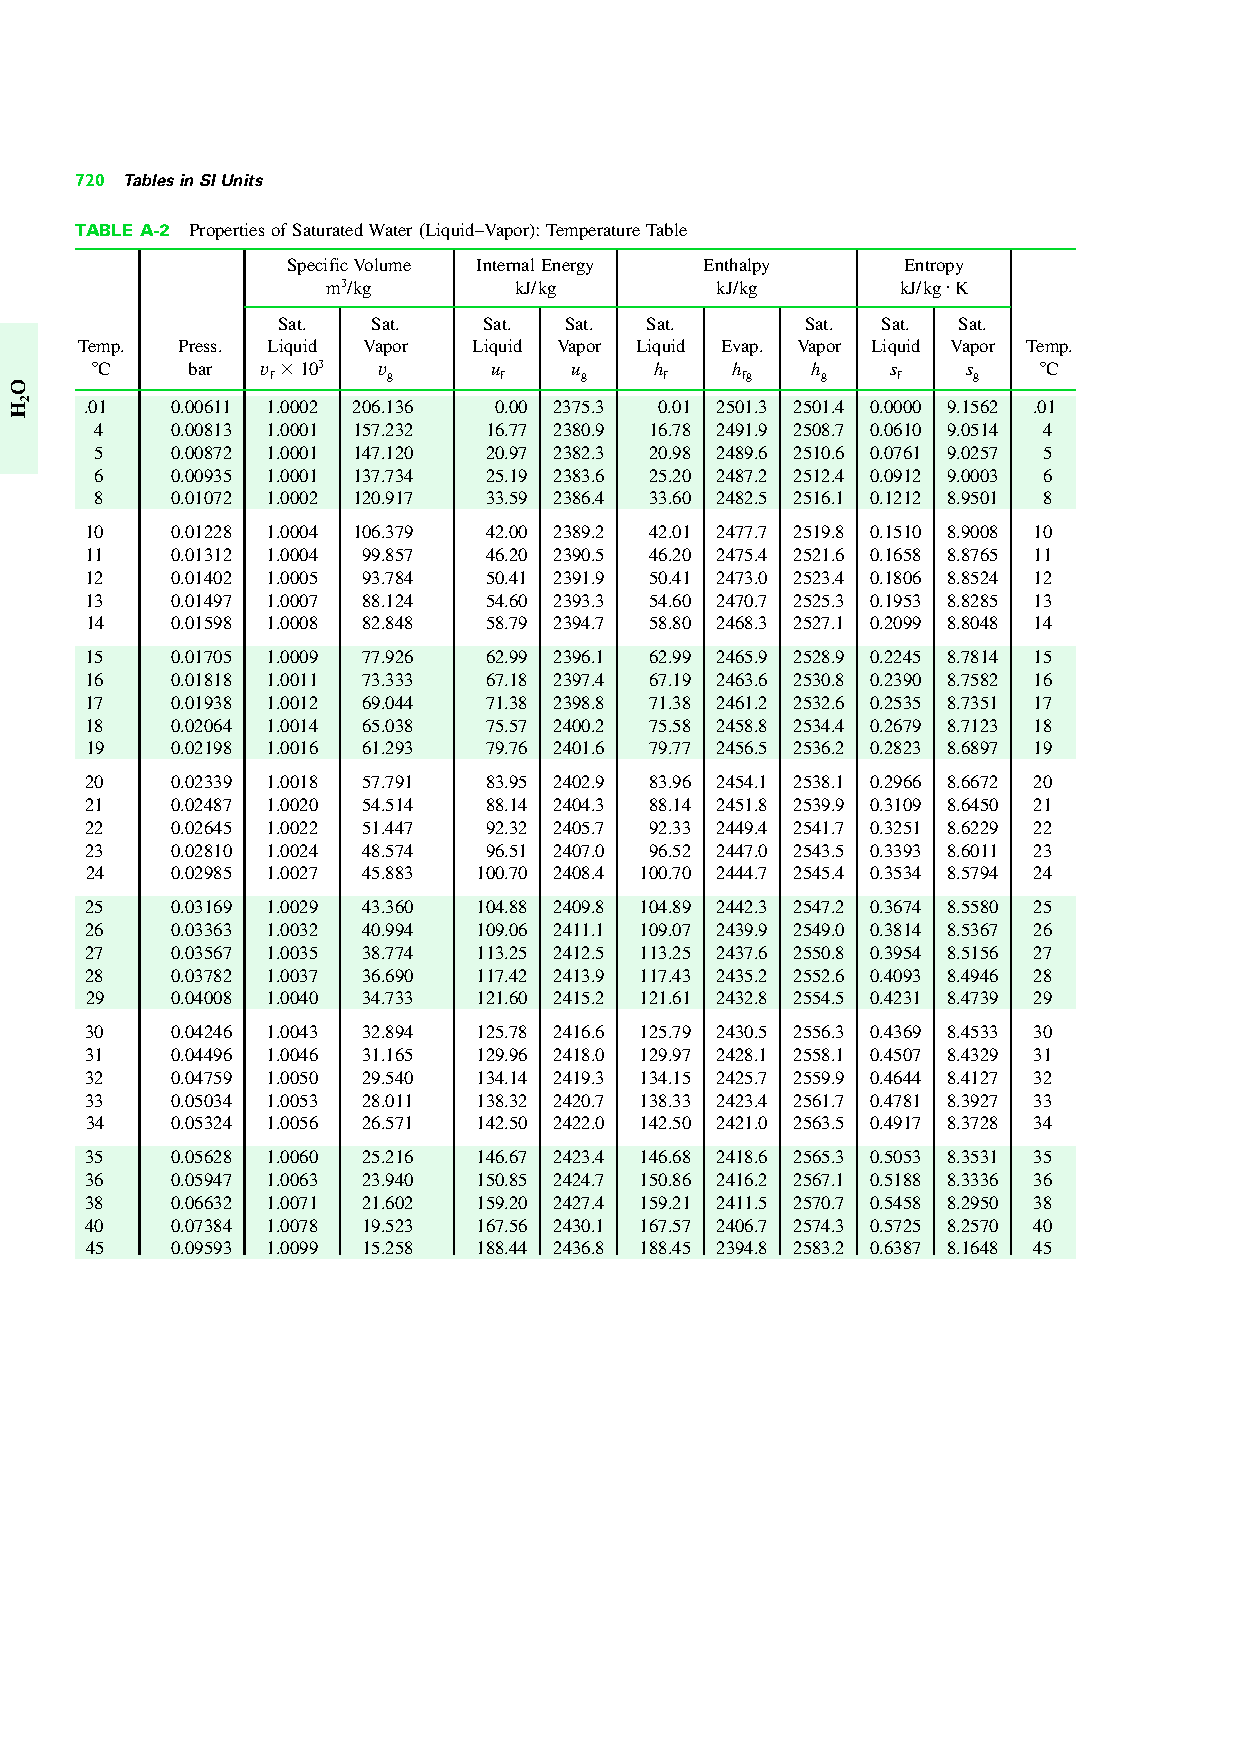
\includepdf[scale=1,pages=-,pagecommand={}, fitpaper]{./Pics/ChemEng_AllTables.pdf}

%       
\chapter{A Few Examples}

\section{Examples}

  \begin{list}{\bf Example \arabic{qcounter}:~}{\usecounter{qcounter}}
%
     %%% EXAMPLE 1:
     \item\label{example1} Using the cyclic rule (Appendix~\ref{Appendix_Calculus:Properties}) and the definitions,
    \begin{displaymath}
        \alpha = \frc{1}{V}\left(\frc{\partial V}{\partial T}\right)_{P} \hspace{1cm}\text{ and }\hspace{1cm} \beta = -\frc{1}{V}\left(\frc{\partial V}{\partial P}\right)_{T},
    \end{displaymath}
    \noindent show that 
    \begin{displaymath}
      \left(\frc{\partial P}{\partial T}\right)_{V} = \frc{\alpha}{\beta}.
    \end{displaymath}
%%
\medskip
     {\bf Solution:} From the cyclic rule,
       \begin{displaymath}
          \left(\frc{\partial P}{\partial T}\right)_{V}\left(\frc{\partial V}{\partial P}\right)_{T}\left(\frc{\partial T}{\partial V}\right)_{T} = -1.
       \end{displaymath}
     Thus,
       \begin{displaymath}
          \left(\frc{\partial P}{\partial T}\right)_{V} = \frc{-1}{\left(\frc{\partial V}{\partial P}\right)_{T}\left(\frc{\partial T}{\partial V}\right)_{T}} = \frc{-\left(\frc{\partial V}{\partial T}\right)_{P}}{\left(\frc{\partial V}{\partial P}\right)_{T}} = \frc{-V\alpha}{-V\beta} = \frc{\alpha}{\beta}
       \end{displaymath}
      
%
     %%% EXAMPLE 2:
     \item\label{example2} For a van der Waals gas, the pressure $P$ and the internal energy $U$ can be expressed as functions of the number of mols ($n$), total volume ($V$) and temperature ($T$),
       \begin{displaymath}
         P = \frc{n R T}{V-nb} - \frc{n^{2}a}{V^{2}} \hspace{1cm}\text{ and }\hspace{1cm} U = \frc{3}{2}n R T - \frc{n^{2}a}{V},
       \end{displaymath}
       respectively, where $a$ and $b$ are constants. Use these equations and the chain rule to derive an equation for $\left(\frc{\partial U}{\partial P}\right)_{n,T}$ in terms of $n$, $V$ and $T$.

%%
\medskip
{\bf Solution:}
   \begin{eqnarray}
      \Partial[U]{P}{n,T} &=& \Partial[U]{V}{n,T}\Partial[V]{P}{n,T} = \frc{\Partial[U]{V}{n,T}}{\Partial[P]{V}{n,T}} \nonumber \\
                          &=& \frc{\frc{n^{2}a}{V^{2}}}{\frc{2n^{2}a}{V^{3}}-\frc{n R T}{\left(V-nb\right)^{2}}} = \frc{n a}{\frc{2 n a}{V}-\frc{R T V^{2}}{\left(V-nb\right)^{2}}}\nonumber
   \end{eqnarray}
      
%
     %%% EXAMPLE 3:
     \item\label{example3} The heat capacity at constant volume is defined as $C_{v}\equiv \Partial[U]{T}{V}$. Show that
       \begin{displaymath}
          \Partial[U]{T}{P} = C_{v} + \alpha V\Partial[U]{V}{T},
       \end{displaymath}
       with $\alpha=\frc{1}{V}\Partial[V]{T}{P}$.

%
\medskip
       {\bf Solution:}
          \begin{displaymath}
            \Partial[U]{T}{P} = \Partial[U]{T}{V} + \Partial[U]{V}{T}\Partial[V]{T}{P},
          \end{displaymath}
          however $\Partial[U]{T}{V}=C_{v}$ and $\Partial[V]{T}{P}=V\alpha$. Thus,
          \begin{displaymath}
             \Partial[U]{T}{P} = C_{v} + \alpha V\Partial[U]{V}{T}.
          \end{displaymath}

%
     %%% EXAMPLE 4:
     \item\label{example4} h
%
\end{list}

\pagebreak

%%%
%%% SECTION
%%%
\section{Quiz}

  \begin{list}{\bf Question \arabic{qcounter}:~}{\usecounter{qcounter}}

%
     %%% QUESTION:
     \item\label{Q1} An experimentalist claims to have raised the temperature of a small amount of water to 150 C by transferring heat from a high temperature steam at 120 C. Is this a reasonable claim? Why? Assume no refrigerator/heat pump is used in the process. 
%

%\medskip
       {\bf Solution:} No. Heat cannot flow from a low temperature medium to a higher temperature medium.

%
     %%% QUESTION:
     \item\label{Q2} What is a thermal energy reservoir? Give examples.
%

%\medskip
       {\bf Solution:} A thermal energy reservoir is a body that can supply or absorb finite quantities of heat isothermally. Some examples are the oceans,lakes, and the atmosphere.
%
     %%% QUESTION:
     \item\label{Q3} Is it possible for a heat engine to operate without rejecting any waste heat to a low temperature reservoir? Explain.
%

%\medskip
       {\bf Solution:} No. Such an engine violates the Kelvin Planck statement of the second law of thermodynamics.

%
     %%% QUESTION:
     \item\label{Q4} What are the characteristics of all heat engines?
%

%\medskip
       {\bf Solution:} Heat engines are cyclic devices that receive heat from a source, convert some of it to work, and reject the rest to a sink.

%
     %%% QUESTION:
     \item\label{Q5} What is the Kelvin Planck expression of the second law of thermodynamics?
%

%\medskip
       {\bf Solution:} "No heat engine can exchange heat with a single reservoir and produce an equivalent amount of work" aka every pair of pants must have two legs
%
     %%% QUESTION:
     \item\label{Q6} Does a heat engine that has a thermal efficiency of 100 percent necessarily violate (a) the first law and (b) the second law of thermodynamics.
%

%\medskip
       {\bf Solution:} (a) No. (b) Yes. According the the second law of thermodynamics, no heat engine can have an efficiency of 100 percent.

%
     %%% QUESTION:
     \item\label{Q7} In the absence of any friction and other irreversibilities, an a heat engine have an efficiency of 100 percent? Explain
%

%\medskip
       {\bf Solution:} No. This violates the second law of thermodynamics.
%
     %%% QUESTION:
     \item\label{Q8} What is the difference between a refrigerator and a heat pump?
%

%\medskip
       {\bf Solution:}  The difference between the two is the purpose of each. The purpose of a refrigerator is to remove heat from a cold medium whereas the purpose of a heat engine is to supply heat to a warm medium.

%
     %%% QUESTION:
     \item\label{Q9} A heat pump is a device that absorbs energy from the cold outdoor air and transfers it to the warmer indoors. Is this a violation of the second law of thermodynamics? Explain.
%

%\medskip
       {\bf Solution:} No. Because the heat pump consumes work to accomplish this task
%
     %%% QUESTION:
     \item\label{Q10} Define the coefficient of performance of a refrigerator in words. Can is be greater than one? 
%

%\medskip
       {\bf Solution:} It represents the amount of heat removed from the refrigerated space for each unit of work supplied. It can be greater than 1

%
     %%% QUESTION:
     \item\label{Q11} A heat pump that is used to heat a house has a COP of 2.5. That is, the heat pump delivers 2.5 kWh of energy to the house for each 1 kWh of electricity it consumes. Does this violate the first law of thermodynamics?
%

%\medskip
       {\bf Solution:} No. The heat pump captures energy from a cold medium and carries it to a warm medium. It does not create it
%
     %%% QUESTION:
     \item\label{Q12} What is the Clausius expression of the second law of thermodynamics?
%

%\medskip
       {\bf Solution:} No device can transfer heat from a cold medium to a warm medium without requiring a heat or work input from the surroundings.

%
     %%% QUESTION:
     \item\label{Q13} Why are engineers interested in reversible processes even though they can never be achieved?
%

%\medskip
       {\bf Solution:} Because reversible processes can be approached in reality, and they form the limiting cases. Work producing devices that operate on reversible processes deliver the most work, and work consuming devices that operate on reversible processes consume the least amount of work.

%
     %%% QUESTION:
     \item\label{Q14} Why does a non-quasi equilibrium compression process require a larger work input than the corresponding quasi equilibrium one?
%

%\medskip
       {\bf Solution:}  When the compression process is non-quasi equilibrium, the molecules before the piston face cannot escape fast enough, forming a high pressure region in front of the piston. It takes more work to more the piston against this higher pressure region.
%
     %%% QUESTION:
     \item\label{Q15} Is a reversible expansion or compression process necessarily quasi equilibrium? Is a quasi equilibrium expansion or compression necessarily reversible?
%

%\medskip
       {\bf Solution:}  A reversible expansion or compression process cannot involve unrestained expansion or sudden compression, and thus it is quasi equilibirum. A quasi equilibirum expansion or compression process, on the other hand, may involve external irreversibilities (like heat transfer through a finite temperature difference) nad thus is not necessarily reversible.

%
     %%% QUESTION:
     \item\label{Q16} What are the four processes that make up the Carnot cycle?
%

%\medskip
       {\bf Solution:}  Isothermal expansion, reversible adiabatic expansion, isothermal compression, reversible adiabatic compression

%
     %%% QUESTION:
     \item\label{Q17} What are the two statements known as the Carnot principles? 
%

%\medskip
       {\bf Solution:} 1. Thermal efficiency of an irreversible heat engine is lower thant the efficiency of a reversible heat engine operating between the same two reservoirs; 2. The thermal efficiency of all the reversible heat engines operating between the same two reservoirs are equal

%
     %%% QUESTION:
     \item\label{Q18} Somebody claims to have developed a new reversible heat engine cycle that has a higher theoretical efficiency than the Carnot cycle operating between the same temperature limits. Is this a reasonable claim? 
%

%\medskip
       {\bf Solution:} No. The second Carnot principle states that no heat engine cycle can have a higher thermal efficiency than the Carnot cycle operating between the same temperature limits.

%
     %%% QUESTION:
     \item\label{Q19} Is it possible to develop (a) an actual and (b) a reversible heat engine cycle that is more efficient that a Carnot cycle operating between the same temperature limits? 
%

%\medskip
       {\bf Solution:} (a) No. (b) No. They would violate the Carnot Principles

%
     %%% QUESTION:
     \item\label{Q20} Somebody claims to have developed a new reversible heat engine that has the the same theoretical efficiency as the Carnot cycle operating between the same temperature limits? Is this a reasonable claim?
%

%\medskip
       {\bf Solution:} Yes. the second Carnot principle states that all reversible heat engine cycles operating between the same temperature limits have the same thermal efficiency.


%
     %%% QUESTION:
     \item\label{Q21} Consider two actual power plants operating with solar energy. Energy is supplied to one plant from a solar pond at 80 C and to the other from concentrating collectors that raise the water temperature to 600 C. Which of these power plants will have a higher efficiency?
%

%\medskip
       {\bf Solution:} The one that has a source temperature of 600 C. This is true because the higher the temperature at which heat is supplied to the working fluid of a heat engine, the higher the thermal efficiency.

%
     %%% QUESTION:
     \item\label{Q22} How can we increase COP of a Carnot refrigerator?
%

%\medskip
       {\bf Solution:} By increasing TL or decreasing TH

%
     %%% QUESTION:
     \item\label{Q23} What is the highest COP that a refrigerator operating between temperature levels TL and TH can have?
%

%\medskip
       {\bf Solution:} It is the COP that a Carnot refrigerator would have, COP=1/(TH/TL -1)

%
     %%% QUESTION:
     \item\label{Q24} In an effort the conserve energy in a heat engine cycle, somebody suggests incorporating a refrigerator that will absorb some of the waste energy QL and transfer it to the energy source of the heat engine. Is this a smart idea?
%

%\medskip
       {\bf Solution:} No. At best (when all is reversible), the increase in the work produced will be equal to the work consumed by the refrigerator. In reality, the work consumed by the refrigerator will always be greater than the additional work produced, resulting in a decrease in the thermal efficiency of the power plant.

%
     %%% QUESTION:
     \item\label{Q25} It is well established that the thermal efficiency of a heat engine increases as the temperature TL at which the heat is rejected from the heat engine decreases. In an effort to increase the efficiency of a power plant, somebody suggest refrigerating the cooling water before it enters the condenser, where heat rejection takes place. Would you be in favor of this idea? Why?
%

%\medskip
       {\bf Solution:} No. At best (when all is reversible), the increase in the work produced will be equal to the work consumed by the refrigerator. In reality, the work consumed by the refrigerator will always be greater than the additional work produced, resulting in a decrease in the thermal efficiency of the power plant.

%
     %%% QUESTION:
     \item\label{Q26} It is well known that the thermal efficiency of heat engines increases as the temperature of the energy source increases. In an attempt to improve the efficiency of a power plant, somebody suggest transferring heat from the available energy source to a higher temperature medium by a heat pump before energy is supplied to the power plant. What do you think of this suggestion?
%

%\medskip
       {\bf Solution:} Bad Idea. At best (all is reversible), the increase in the work produced will equal the work consumed by the heat pump. In reality, the work consumed by the heat pump will always be greater than the additional work produced, resulting in a decrease in the thermal efficiency of the power plant.

%
     %%% QUESTION:
     \item\label{Q27} Does the temperature in the Clausius inequality relation have to be absolute temperature? Why?
%

%\medskip
       {\bf Solution:} Yes. Because we used the relation (QH/TH=QL/TL) in the proof, which is the defining relation of absolute temperature.

%
     %%% QUESTION:
     \item\label{Q28} Does a cycle for which deltaQ>0 violate the Clausius inequality? 
%

%\medskip
       {\bf Solution:} No. The deltaQ represents the net heat transfer during a cycle, would could be positive

%
     %%% QUESTION:
     \item\label{Q29} Does the cyclic integral of heat have to be zero (i.e. does a system have to reject as much heat as it consumes to complete a cycle)? 
%

%\medskip
       {\bf Solution:} No. A system may reject more or less heat than it receives during a cycle. The steam in a steam power plant, for example, received more heat than it rejects in a cycle.

%
     %%% QUESTION:
     \item\label{Q30} Does the cyclic integral of work have to be zero (i.e. does a system have to produce as much work as it consumes to complete a cycle)? 
%

%\medskip
       {\bf Solution:} No. A system may produce more or less work than it receives during a cycle. A steam power plant for example, produces more work than it receives during a cycle, the difference being the the net work output.

%
     %%% QUESTION:
     \item\label{Q31} A system undergoes a process between two fixed states first in a reversible manner and then in an irreversible manner. For which case is the entropy change greater?
%

%\medskip
       {\bf Solution:} The entropy change will be the same for both cases since the entropy is a a property and it has a fixed value at a fixed state.

%
     %%% QUESTION:
     \item\label{Q32} Is the value of the integral, from 1 to 2, of deltaQ/T the same for all processes between states one and two?
%

%\medskip
       {\bf Solution:} No. In general, that integral will have a different value for different processes. However, it will have the same value for all reversible processes.

%
     %%% QUESTION:
     \item\label{Q33} Is the value of the integral, from 1 to 2, of deltaQ/T the same for all reversible processes between states one and two?
%

%\medskip
       {\bf Solution:} Yes

%
     %%% QUESTION:
     \item\label{Q34} To determine the entropy change for an irreversible process between states one and two, should the integral, from 1 to 2, of deltaQ/T be performed along the actual process path or an imaginary reversible path?
%

%\medskip
       {\bf Solution:} That integral would be performed along a reversible path to determine the entropy change

%
     %%% QUESTION:
     \item\label{Q35} Is an isothermal process necessarily internally reversible? Give an example.
%

%\medskip
       {\bf Solution:} No. An isothermal process and be irreversible. For example, a system that involves paddle wheel work while losing an equivalent amount of heat.

%
     %%% QUESTION:
     \item\label{Q36} How do the values of the integral, from 1 to 2, of deltaQ/T compare for a reversible and irreversible process between the same end states? 
%

%\medskip
       {\bf Solution:} The value of this integral is always larger for reversible processes

%
     %%% QUESTION:
     \item\label{Q37} A piston cylinder device contains helium gas. During a reversible, isothermal process, the entropy of the helium will increase ...
%

%\medskip
       {\bf Solution:} Sometimes

%
     %%% QUESTION:
     \item\label{Q38} A piston cylinder device contains nitrogen gas. During a reversible, adiabatic process, the entropy of the nitrogen will increase
%

%\medskip
       {\bf Solution:} Never

%
     %%% QUESTION:
     \item\label{Q39} A piston cylinder device contains superheated steam. During an actual, adiabatic process, the entropy of the steam will increase.
%

%\medskip
       {\bf Solution:} Always

%
     %%% QUESTION:
     \item\label{Q40} The entropy of steam will ... as it flows through an actual adiabatic turbine.
%

%\medskip
       {\bf Solution:} Increase

%
     %%% QUESTION:
     \item\label{Q41} The entropy of the working fluid of the ideal Carnot cycle ... during the isothermal heat addition process.
%

%\medskip
       {\bf Solution:} Increase

%
     %%% QUESTION:
     \item\label{Q42} The entropy of the working fluid of the ideal Carnot cycle ... during the isothermal heat rejection process
%

%\medskip
       {\bf Solution:} Decreases

%
     %%% QUESTION:
     \item\label{Q43} During a heat transfer process, the entropy of a system ... increases
%

%\medskip
       {\bf Solution:} Sometimes

%
     %%% QUESTION:
     \item\label{Q44} Is it possible for the entropy change of a closed system to be zero during an irreversible process?
%

%\medskip
       {\bf Solution:} Yes. This will happen when the system is losing heat, and the decrease in entropy as a result of this heat loss is equal in entropy as a result of irreversibilities.

%
     %%% QUESTION:
     \item\label{Q45} Is a process that is internally reversible and adiabatic necessarily isentropic? 
%

%\medskip
       {\bf Solution:} Yes, because an internally reversible, adiabatic process invovles no irreversibilities or heat transfer
%
     %%% QUESTION:
     \item\label{Q46} Consider two sold blocks, one hot and one cold, brought into contsant in an adiabatic container. After a while, thermal equilibrium is established in the container as a result of heat transfer. The first law requires that the amount of energy lost by the hot solid be equal to the amount of energy gained by the cold one. Does the second law require that the decrease in entropy of the hot solid be equal to the increase in entropy of the cold one?
%

%\medskip
       {\bf Solution:} No, because entropy is not a conserved property

%
     %%% QUESTION:
     \item\label{Q47} Can entropy of an ideal gas change during an isothermal process? 
%

%\medskip
       {\bf Solution:} The entorpy of a gas can change during an isothermal process since entropy of an ideal gas depends on the pressure as well as the temperature.

%
     %%% QUESTION:
     \item\label{Q48} An ideal gas undergoes a process between two specifes temperatures, first at constant pressure and then at constant volume. For which case will the ideal gas experience a larger entropy change? 
%

%\medskip
       {\bf Solution:} The entropy change relations of an ideal gas simplify to: 1. delta s=Cpln(T2/T1) for a constant pressure process 2. delta s=Cvln(T2/T1) for a constant volume process 3 noting that Cp>Cv. the entropy change will be larger for a constant pressure process

%
     %%% QUESTION:
     \item\label{Q49} Describe the ideal process for an (a) adiabatic turbine, (b) adiabatic compressor, and (c) adiabatic nozzle, and define the isentropic efficiency for each device.
%

%\medskip
       {\bf Solution:} The ideal process for all three devices is the reversible adiabatic (i.e. isentropic) process. The isentropic efficincies can be defined as: 1. eta(turbine, isentropic)= actual work output/isentropic work output 2. eta(compressor,isentopic)=isentropic work input/ actual work input 3. eta(nozzle,isentropic)=actual exit kinetic energy/ isentropic exit kinetic energy


%
     %%% QUESTION:
     \item\label{Q50} Is the isentropic process a suitable model for compressors that are cooled intentionally? 
%

%\medskip
       {\bf Solution:} No, because the isentropic process is not the model or ideal process for compressors that are cooled unintentionallly.

%
     %%% QUESTION:
     \item\label{Q51} On a T-s diagram, does the actual exit state (state 2) of an adiabatic turbine have to be on the right hand side of the isentropic exit state (state 2s)?
%

%\medskip
       {\bf Solution:} Yes. Because the entropy of the fluid must increase during an actual adiabatic process as a result of irreversibilities. Therefore, the actual exit state has to be on the right hand side of the isentropic exit state.

%
\end{list}

  \end{appendix}

\cleardoublepage

\pagebreak

\bibliographystyle{plainnat}
\bibliography{refbib}
%\bibliographystyle{unsrt}

\cleardoublepage
\phantomsection
\renewcommand\leftmark{}
\renewcommand\rightmark{Index}
\addcontentsline{toc}{chapter}{Index}

\printindex


\end{document}
